\documentclass{dukedissertation}
%\documentclass[economy,twoside,bind]{dukedissertation}

% Other useful options (there are more options documented in Chapter 2):
%  * draft -- don't actually include images, print a black bar on overful
%             hboxes
%  * MS    -- Format for a Master's Thesis.  No UMI abstract page, some
%             textual changes to title page.


% Useful packages for dissertation writing:
% align, gather, multiline, etc.
\usepackage[overload]{empheq}

% frequently used symbols
\usepackage{amssymb}

% additional math fonts
\usepackage{mathrsfs}

% frequently used theorems
\usepackage{amsthm}

% programatically typeset units
\usepackage{siunitx}

% graphics
\usepackage{graphicx}

% put stuff over a figure
\usepackage{overpic}

% reenable multidot in graphic file name
\usepackage{grffile}

% additional color definitions
\usepackage[dvipsnames]{xcolor}

% framed text environment with pagebreak
\usepackage{mdframed}

% multicolumn environment
\usepackage{paracol}
\columnratio{0.5}

% algorithm
\usepackage{algorithm}
\usepackage{algpseudocode}

% additional control over appendices
\usepackage[title,titletoc]{appendix}

% additional control over captions
\usepackage[font=small,labelfont=bf,labelsep=period,width=.9\textwidth]{caption}

% subfigure
\usepackage{subcaption}

% typeset hyperlinks
\usepackage[pdftex, pdfusetitle, plainpages=false,
  bookmarks, bookmarksnumbered,
  colorlinks, linkcolor=black, citecolor=black,
  filecolor=black, urlcolor=black]
{hyperref}

% clever cross-referencing tool
\usepackage{cleveref}

% extended table formatting
\usepackage{array}
\usepackage{booktabs}

% additional control over enum items
\usepackage{enumitem}

% string manipulation
\usepackage{stringstrings}
\usepackage{xstring}

% set spacing and stretch
\usepackage{setspace}

% for non-italic greek letters
\usepackage{upgreek}

\usepackage{pgfplots}
\pgfplotsset{compat=1.16}

% additional color cycle list
\usepgfplotslibrary{colorbrewer}
\usepgfplotslibrary{colormaps}
\usepgfplotslibrary{fillbetween}
\usepgfplotslibrary{groupplots}

% additional tikz libraries
\usetikzlibrary{patterns}
\usetikzlibrary{spy}

% style to select only points from #1 to #2 (inclusive)
\pgfplotsset{select coords between index/.style 2 args={
      x filter/.code={
          \ifnum\coordindex<#1\def\pgfmathresult{}\fi
          \ifnum\coordindex>#2\def\pgfmathresult{}\fi
        }
    }}

\usepackage{tikz}

% externalize tikz to avoid unnecessary recompilation of complicated figures
\usetikzlibrary{external}
\tikzexternalize[prefix=tikz/]

\newcommand{\tikzsetnextfilenamesafe}[1]{
  \StrSubstitute{#1}{/}{-}[\temp]
  \tikzsetnextfilename{\temp}
}

% convenient bold symbols
\newcommand{\bfa}{\boldsymbol{a}}
\newcommand{\bfb}{\boldsymbol{b}}
\newcommand{\bfc}{\boldsymbol{c}}
\newcommand{\bfd}{\boldsymbol{d}}
\newcommand{\bfe}{\boldsymbol{e}}
\newcommand{\bff}{\boldsymbol{f}}
\newcommand{\bfg}{\boldsymbol{g}}
\newcommand{\bfh}{\boldsymbol{h}}
\newcommand{\bfi}{\boldsymbol{i}}
\newcommand{\bfj}{\boldsymbol{j}}
\newcommand{\bfk}{\boldsymbol{k}}
\newcommand{\bfl}{\boldsymbol{l}}
\newcommand{\bfm}{\boldsymbol{m}}
\newcommand{\bfn}{\boldsymbol{n}}
\newcommand{\bfo}{\boldsymbol{o}}
\newcommand{\bfp}{\boldsymbol{p}}
\newcommand{\bfq}{\boldsymbol{q}}
\newcommand{\bfr}{\boldsymbol{r}}
\newcommand{\bfs}{\boldsymbol{s}}
\newcommand{\bft}{\boldsymbol{t}}
\newcommand{\bfu}{\boldsymbol{u}}
\newcommand{\bfv}{\boldsymbol{v}}
\newcommand{\bfw}{\boldsymbol{w}}
\newcommand{\bfx}{\boldsymbol{x}}
\newcommand{\bfy}{\boldsymbol{y}}
\newcommand{\bfz}{\boldsymbol{z}}

\newcommand{\bfA}{\boldsymbol{A}}
\newcommand{\bfB}{\boldsymbol{B}}
\newcommand{\bfC}{\boldsymbol{C}}
\newcommand{\bfD}{\boldsymbol{D}}
\newcommand{\bfE}{\boldsymbol{E}}
\newcommand{\bfF}{\boldsymbol{F}}
\newcommand{\bfG}{\boldsymbol{G}}
\newcommand{\bfH}{\boldsymbol{H}}
\newcommand{\bfI}{\boldsymbol{I}}
\newcommand{\bfJ}{\boldsymbol{J}}
\newcommand{\bfK}{\boldsymbol{K}}
\newcommand{\bfL}{\boldsymbol{L}}
\newcommand{\bfM}{\boldsymbol{M}}
\newcommand{\bfN}{\boldsymbol{N}}
\newcommand{\bfO}{\boldsymbol{O}}
\newcommand{\bfP}{\boldsymbol{P}}
\newcommand{\bfQ}{\boldsymbol{Q}}
\newcommand{\bfR}{\boldsymbol{R}}
\newcommand{\bfS}{\boldsymbol{S}}
\newcommand{\bfT}{\boldsymbol{T}}
\newcommand{\bfU}{\boldsymbol{U}}
\newcommand{\bfV}{\boldsymbol{V}}
\newcommand{\bfW}{\boldsymbol{W}}
\newcommand{\bfX}{\boldsymbol{X}}
\newcommand{\bfY}{\boldsymbol{Y}}
\newcommand{\bfZ}{\boldsymbol{Z}}

\newcommand{\bta}{\textbf{a}}
\newcommand{\btb}{\textbf{b}}
\newcommand{\btc}{\textbf{c}}
\newcommand{\btd}{\textbf{d}}
\newcommand{\bte}{\textbf{e}}
\newcommand{\btf}{\textbf{f}}
\newcommand{\btg}{\textbf{g}}
\newcommand{\bth}{\textbf{h}}
\newcommand{\bti}{\textbf{i}}
\newcommand{\btj}{\textbf{j}}
\newcommand{\btk}{\textbf{k}}
\newcommand{\btl}{\textbf{l}}
\newcommand{\btm}{\textbf{m}}
\newcommand{\btn}{\textbf{n}}
\newcommand{\bto}{\textbf{o}}
\newcommand{\btp}{\textbf{p}}
\newcommand{\btq}{\textbf{q}}
\newcommand{\btr}{\textbf{r}}
\newcommand{\bts}{\textbf{s}}
\newcommand{\btt}{\textbf{t}}
\newcommand{\btu}{\textbf{u}}
\newcommand{\btv}{\textbf{v}}
\newcommand{\btw}{\textbf{w}}
\newcommand{\btx}{\textbf{x}}
\newcommand{\bty}{\textbf{y}}
\newcommand{\btz}{\textbf{z}}

\newcommand{\btA}{\textbf{A}}
\newcommand{\btB}{\textbf{B}}
\newcommand{\btC}{\textbf{C}}
\newcommand{\btD}{\textbf{D}}
\newcommand{\btE}{\textbf{E}}
\newcommand{\btF}{\textbf{F}}
\newcommand{\btG}{\textbf{G}}
\newcommand{\btH}{\textbf{H}}
\newcommand{\btI}{\textbf{I}}
\newcommand{\btJ}{\textbf{J}}
\newcommand{\btK}{\textbf{K}}
\newcommand{\btL}{\textbf{L}}
\newcommand{\btM}{\textbf{M}}
\newcommand{\btN}{\textbf{N}}
\newcommand{\btO}{\textbf{O}}
\newcommand{\btP}{\textbf{P}}
\newcommand{\btQ}{\textbf{Q}}
\newcommand{\btR}{\textbf{R}}
\newcommand{\btS}{\textbf{S}}
\newcommand{\btT}{\textbf{T}}
\newcommand{\btU}{\textbf{U}}
\newcommand{\btV}{\textbf{V}}
\newcommand{\btW}{\textbf{W}}
\newcommand{\btX}{\textbf{X}}
\newcommand{\btY}{\textbf{Y}}
\newcommand{\btZ}{\textbf{Z}}


% textual mathematical operators
\DeclareMathOperator{\tr}{tr}
\DeclareMathOperator{\dev}{dev}
\DeclareMathOperator*{\argmin}{arg\,min}
\DeclareMathOperator*{\argmax}{arg\,max}
\DeclareMathOperator{\sgn}{sgn}
\DeclareMathOperator{\diag}{diag}
\DeclareMathOperator{\mathspan}{span}
\DeclareMathOperator{\cov}{C}
\DeclareMathOperator{\cor}{R}
\DeclareMathOperator{\cof}{cof}
\DeclareMathOperator{\sym}{sym}

% miscellaneous operators
\newcommand{\diff}[1]{\text{ d}#1}
\newcommand{\evalover}[1]{\left\vert_{#1}\right.}
\newcommand{\grad}{\bs{\nabla}}
\newcommand{\divergence}{{\grad \cdot}}
\newcommand{\wbigcup}{\mathop{\bigcup}\displaylimits}
\newcommand{\norm}[1]{\left\lVert#1\right\rVert}
\newcommand{\macaulay}[1]{\left<#1\right>}
\newcommand{\bs}[1]{\boldsymbol{#1}}
\newcommand{\abs}[1]{\left\vert{#1}\right\vert}
\newcommand{\overbar}[1]{\mkern 1.5mu\overline{\mkern-1.5mu#1\mkern-1.5mu}\mkern 1.5mu}
\newcommand{\exponential}[1]{\exp\left(#1\right)}

% for elasticity
\newcommand{\stress}{\boldsymbol{\sigma}}
\newcommand{\xstress}{\widetilde{\stress}}
\newcommand{\strain}{\boldsymbol{\varepsilon}}
\newcommand{\normal}{\btn}
\newcommand{\xnormal}{\widetilde{\normal}}
\newcommand{\defgrad}{\bfF}
\newcommand{\defrate}{\dot{\bs{\upphi}}}

% for fracture
\newcommand{\crackset}{\Gamma}
\newcommand{\Gc}{{\mathcal{G}_c}}
\newcommand{\activepart}{{\left< A \right>}}
\newcommand{\inactivepart}{{\left< I \right>}}

% for plasticity
\newcommand{\ep}{{\overbar{\varepsilon}^p}}
\newcommand{\epdot}{{\dot{\overbar{\varepsilon}}^p}}

% utility typography for consistency
\newcommand{\field}[1]{\mathbb{#1}}
\newcommand{\set}[1]{#1}
\newcommand{\fspace}[1]{\mathcal{#1}}
\newcommand{\body}{\set{\Omega}}
\newcommand{\bodyboundary}{{\partial \body}}

% superscripts and subscripts
\newcommand{\total}{\text{total}}
\newcommand{\internal}{\text{internal}}
\newcommand{\external}{\text{external}}
\newcommand{\fracture}{\text{fracture}}
\newcommand{\elastic}{\text{elastic}}
\newcommand{\critical}{\text{critical}}
\newcommand{\potential}{\text{potential}}
\newcommand{\plastic}{\text{plastic}}
\newcommand{\trial}{\text{trial}}

% mark something as DONE or TODO
\newcommand\Done{\textcolor{ForestGreen}{\textbf{ [DONE] }}}
\newcommand\ToDo{\textcolor{Red}{\textbf{ [TODO] }}}

% my preferred alternative environment
\theoremstyle{definition}
\newtheorem*{mdalternative}{Alternative}
\definecolor{alternativegray}{gray}{0.95}
\newenvironment{alternative}%
{\begin{mdframed}[backgroundcolor=alternativegray,linewidth=0pt,startinnercode={\baselineskip=0.8cm}]\begin{mdalternative}\vspace{-0.5em}}
      {\end{mdalternative}\end{mdframed}}

% my preferred example environment
\theoremstyle{definition}
\newtheorem{mdexample}{Example}
\definecolor{examplegray}{gray}{0.95}
\newenvironment{example}%
{\begin{mdframed}[backgroundcolor=examplegray,linewidth=0pt,startinnercode={\baselineskip=0.8cm}]\begin{mdexample}\vspace{-0.5em}}
      {\end{mdexample}\end{mdframed}}

% my preferred remark environment
\theoremstyle{definition}
\newtheorem{mdremark}{Remark}
\definecolor{remarkgray}{gray}{0.95}
\newenvironment{remark}%
{\begin{mdframed}[backgroundcolor=remarkgray,linewidth=0pt,startinnercode={\baselineskip=0.8cm}]\begin{mdremark}\vspace{-0.5em}}
      {\end{mdremark}\end{mdframed}}
\crefname{remark}{remark}{remarks}

\usepackage[numbers]{natbib}

%-----------------------------------------------------------------------------%
% PREAMBLE
%-----------------------------------------------------------------------------%
\setcounter{secnumdepth}{3}
\setcounter{tocdepth}{2}
\author{Tianchen Hu}
\title{A Variational Framework for Phase-Field Fracture Modeling with Applications to Fragmentation, Desiccation, Ductile Failure, and Spallation}
\supervisor{John Dolbow}
\department{Mechanical Engineering and Materials Science} % Appears as Department of \department
% Declare dissertation subject used on UMI abstract page.  List of
% categories: http://dissertations.umi.com/duke/subject_categories.html
%\subject{[Your Subject Here]}

\date{2021} % Anything but the year is ignored.

% Copyright text.  If undefined, default is 'All rights reserved'
% (Example sets the text to a hyperlinked Creative Commons Licence)
% \copyrighttext{ All rights reserved except the rights granted by the\\
%   \href{http://creativecommons.org/licenses/by-nc/3.0/us/}
%         {Creative Commons Attribution-Noncommercial Licence}
%}

% Committee Members other than supervisor.  No more than five beyond the
% supervisor allowed.
\member{Wilkins Aquino}
\member{Johann Guilleminot}
\member{Manolis Veveakis}
\member{Benjamin W. Spencer}
%-----------------------------------------------------------------------------%

\begin{document}

%-----------------------------------------------------------------------------%
% TITLE PAGE -- provides UMI abstract title page & copyright if appropriate
%-----------------------------------------------------------------------------%
\maketitle

%-----------------------------------------------------------------------------%
% ABSTRACT -- included file should start with '\abstract'.
%-----------------------------------------------------------------------------%
\abstract

Fracture is a common phenomenon in engineering applications. Many types of fracture exist, including, but not limited to, brittle fracture, quasi-brittle fracture, cohesive fracture, and ductile fracture. Predicting fracture has been one of the most challenging research topics in computational mechanics. The variational treatment of fracture and its associated phase-field regularization have been employed with great success for modeling fracture in brittle materials. Extending the variational statement to describe other types of fracture and coupled field phenomena has proven less straightforward. Main challenges that remain include how to best construct a total potential that is both mathematically sound and physically admissible, and how to properly describe the coupling between fracture and other physics.

The research presented in this dissertation aims at addressing the aforementioned challenges. A variational framework is proposed to describe fracture in general dissipative solids. In essence, the variational statement is extended to account for large deformation kinematics, inelastic deformation, dissipation mechanisms, dynamic effects, and thermal effects. The proposed variational framework is shown to be consistent with conservations and laws of thermodynamics, and it provides guidance and imposes restrictions on the construction of models for coupled field problems. Within the proposed variational framework, several models are instantiated to address practical engineering problems. A brittle and quasi-brittle fracture model is used to investigate fracture evolution in polycrystalline materials; a cohesive fracture model is applied to revisit soil desiccation; a novel ductile fracture model is proposed and successfully applied to simulate some challenging benchmark problems; and a creep fracture model is developed to simulate the spallation of oxide scale on high temperature heat exchangers.


%-----------------------------------------------------------------------------%
% DEDICATION -- OPTIONAL.  Put the text inside the braces.
%               (Long 'dedications' probably belong in the acknowledgements)
%-----------------------------------------------------------------------------%
%\dedication{If you want to dedicate your thesis to anyone do so here}

%-----------------------------------------------------------------------------%
% FRONTMATTER -- ToC is required, LoT and LoF are required if you have any
% tables or figures, respectively. List of Abbreviations and Symbols is
% optional.
%-----------------------------------------------------------------------------%
\tableofcontents % Automatically generated
\listoftables	% If you have any tables, automatically generated
\listoffigures	% If you have any figures, automatically generated

%-----------------------------------------------------------------------------%
% ACKNOWLEDGEMENTS -- included file should start with '\acknowledgements'
%-----------------------------------------------------------------------------%
\acknowledgements

I am thankful for the many people.


%==============================================================================
%-----------------------------------------------------------------------------%
% MAIN BODY OF PAPER
%-----------------------------------------------------------------------------%
\chapter{Introduction}
\label{section: intro}

Introduction placeholder.

\section{Background}

%% Fracture mechanics basics
In this dissertation, four types of fracture are of interest: brittle fracture, quasi-brittle fracture, cohesive fracture, and ductile fracture. Brittle and quasi-brittle fracture center around the Griffith-type description of fracture, in the sense that the stress field at the crack tip is singular. In particular, brittle fracture is characterized with the complete loss of tensile strength upon crack nucleation. Under displacement-controlled uni-axial tension, a brittle specimen forms a through crack immediately after crack nucleation. Quasi-brittle fracture, in contrast, shows a gradual decay of tensile stress which is often measured in the form of a traction-separation law. Although the celebrated Griffith theory of fracture captures the behavior of wide range of brittle and quasi-brittle materials, it bears emphasis that most materials are not perfectly brittle in the Griffith sense. Cohesive fracture, for example, describes materials that possess a \emph{fracture process zone} ahead of the crack tip. The fracture process zone (FPZ) is a lumped description of small-scale yielding, void coalescence, and micro-crack merging. Typically, the material inside the FPZ only partially loses its load-carrying capacity, and therefore cohesive fracture also displays a gradual decay of tensile stress after crack initiation. The boundary between the definitions of quasi-brittle fracture and cohesive fracture is inherently vague. In this dissertation, cohesive fracture is assumed to have a substantially larger fracture process zone than quasi-brittle fracture, and at the engineering scale, numerical models for these two types of fracture are often used interchangeably. Lastly, ductile fracture describes the softening due to fracture after the stage of plastic hardening. Most metals and fiber-reinforced cementitious composites are ductile and are subject to ductile failure,

%% Briefly mention other methods to model fracture
A number of models have been proposed to model fracture. In what follows is a brief, non-comprehensive survey of numerical methods to model fracture. Particle-based and mesh-free discretization techniques, such as discrete element method (DEM), lattice spring methods, peridynamics theory, have been developed for fracture modeling. The key advantage of these methods lies in the fact that cracks can nucleate and grow in an unguided manner. However, the computational cost of these methods can be very high and the interface conditions are not straightforward to apply. Within the context of the finite element method (FEM), linear elastic fracture mechanics models are extensively used, among which the most commonly used methods are the extended finite element method (XFEM) and the cohesive zone method (CZM). In XFEM, cracks are represented as discrete discontinuities and the displacements with discontinuities are enriched using the partition of unity method \cite{babuaka1997, Dolbow99}. Singularities associated with fracture can be represented using XFEM enrichment at relatively low costs. However, tracking the evolution of complex fracture surfaces, particularly in 3D, is quite tedious. In CZM, damage evolution is governed by a traction-separation law at crack surfaces \cite{needleman_1992, ortiz_1999}. For polycrystalline material, CZM can explicitly account for grain boundaries and model intergranular crack initiation and evolution \cite{KAMAYA2007, KAMAYA2009}. Nonetheless, CZM suffers from mesh dependency because the representation of crack propagation is restricted to element boundaries.

%% Origin of phase-field fracture models and how it works
The variational approach to fracture was proposed by \citet{Francfort98}, and the phase-field implementation is attributed to \citet{Bourdin2000}.
\citet{bourdin2008variational} provides an overview.  In the variational approach, crack surfaces are represented by a surface density function in terms of an auxiliary phase-field. This naturally gives rise to a regularization involving a length scale parameter. Recent works have illustrated potential of phase-field models to be predictive for a wide range of fracture problems. Phase-field for fracture models have succeeded in capturing complex crack patterns, including branching and merging in both two and three dimensions \cite{karma_2001, karma_2004, henry_2004, spatschek_2007, amor_2009}.

%% Seminal works on the variational framework
The general variational framework was first proposed by \citet{biot1956thermoelasticity} in the context of thermoelasticity, followed by extensive investigations in coupled thermoelastic and thermoviscoelastic systems \cite{herrmann1963variational,ben1965variational,oden2012variational,molinari1987global,batra1989principle,matsubara2021variationally}. Well-defined variational principles for dissipative solids with and without heat conduction also exist \cite{ortiz_1999,yang2006variational}. However, the case of thermo-mechanical-fracture coupling in dissipative materials has received far less attention.

%% What variational really means
It is worth noting that there are fundamental differences between variational consistency and thermodynamic consistency. In fact, thermodynamically consistent models are not necessarily variational. To satisfy thermodynamics, the model \emph{must} satisfy the mass conservation, linear momentum conservation, angular momentum conservation, as well as the first and the second laws of thermodynamics. Violating any of the aforementioned conservations or thermodynamic laws results in a physically inadmissible model. However, since the second law of thermodynamics is an inequality statement, there are infinitely many ways to satisfy it when modeling a dissipative solid. In contrast, the variational approach (including, but not limited to, variational approaches to fracture) is based on the idea that, upon careful construction of a potential, its variational statements are thermodynamically consistent, implying that the dissipation attains its maximum at the solution corresponding the variational statements. In other words, the variational approach sets a more restrictive stage for model construction because it places more constraints on the constitutive behavior of the material. For example, if a potential is constructed within the variational framework to account for thermomechanical coupling, the heat generation due to its dissipation is directly predicted by the variational statement and cannot be specified arbitrarily.

%% Benefits of a variational model
The restrictions imposed by the variational approach lead to several beneficial aspects. First, the variational framework enables application of the tools of calculus of variations to the analysis of the solutions of the problem. In particular, direct method of calculus of variations informs conditions for the existence and uniqueness of solutions (e.g. \cite{dal2012introduction}). Second, localization of fracture and plastic zone can be studied within the framework of free-discontinuity problems \cite{braides1998approximation,gariepy2001functions}. Third, in numerical methods, discretization of the variational statement of the problem leads to a symmetric operator, which can save storage and potentially accelerates the assembly process. Furthermore, energy-based line search methods can be directly applied to the system of equations; many powerful numerical optimization packages (e.g. PETSc \cite{petsc-web-page}, TAO \cite{benson2003tao}, Trilinos \cite{heroux2005overview}, and Matlab \cite{higham2016matlab}) can be utilized out-of-the-box; the time-discretized variational problem leads to robust and efficient variational constitutive update algorithms \cite{ortiz_1999}.


\section{Organization of the dissertation}

First, the variational framework is presented in \Cref{section: Chapter2}. General kinematics and constraints assumed throughout this dissertation are summarized in \Cref{section: Chapter2/kinematics}. \Cref{section: Chapter2/thermodynamics} provides a brief review of thermodynamic conservations and laws in their global and local forms.
The proposed variational framework is presented in \Cref{section: Chapter2/minimization}, and discretization of the governing equations is presented in \Cref{section: Chapter2/discretization}.

The variational framework is applied to solve engineering problems in \Cref{section: Chapter3,section: Chapter4,section: Chapter5}. \Cref{section: Chapter3} simulates intergranular fracture and fission-gas-induced fracture in microstructures. \Cref{section: Chapter4} revisits the soil desiccation problem and explores the effect of random fracture properties. \Cref{section: Chapter5} benchmarks the ductile fracture model with a three-point bending experiment and one of the Sandia Fracture Challenges, and models oxide spallation in high-temperature heat exchangers. Each chapter begins with a general introduction to provide context and an overview of state-of-the-art methods and models. Then, the specific constitutive choices are made, and the resulting governing equations are presented. Each chapter is concluded with verifications of the variational model and some concrete numerical examples.


\section{Notation}

In what follows, deterministic scalar, vectors, second-order tensors, and fourth-order tensors are denoted by $a$ (or $A$), $\bta$ (or $\btA$), $\bfA$, and $\mathbb{A}$, respectively.

Let $\body$ be a collection of points $\btX \in \mathbb{R}^d$, $d \in \{1, 2, 3\}$. Scalar- and vector-valued random fields defined on the probability space $(\Theta, \Sigma, P)$, indexed by $\body$, are denoted as $\{ A(\btX), \btX \in \body \}$ and $\{ \btA(\btX), \btX \in \body \}$, respectively.
At any fixed material point $\btX \in \body$, $a(\btX)$ and $\bta(\btX)$ are random variables defined on the probability space $(\Theta, \Sigma, P)$. For any fixed $\theta \in \Theta$, $a(\theta)$ and $\bta(\theta)$ are realizations of the random variables.
Similarly, $\btX \mapsto a(\btX;\theta)$ and $\btX \mapsto \bta(\btX;\theta)$ are realizations of the random fields $\{ A(\btX), \btX \in \body \}$ and $\{ \btA(\btX), \btX \in \body \}$.

Einstein summations are assumed wherever applicable unless otherwise stated. For any vectors $\bta$ and $\btb$ of the same size, the inner product is defined as $\bta \cdot \btb = a_ib_i$ where $a_i$ and $b_i$ are components of the vectors. The associated vector norm is $\norm{\bta}^2 = \bta \cdot \bta$. Similarly, for any second-order tensors $\bfA$ and $\bfB$ of the same size, the inner product is defined as $\bfA : \bfB = \tr(\bfA^T \bfB)$. The associated Frobenius norm reads $\norm{\bfA} = \sqrt{\bfA : \bfA}$. Other matrix norms will be distinguished by subscripts.
The outer (cross) product of two vectors is written as $\bta \otimes \btb = a_ib_j$. The time derivative is denoted by an over-dot, e.g. $\dot{a}$.

Macaulay brackets are denoted by triangle brackets $\macaulay{a}_\pm$ and are defined as $\macaulay{a}_\pm \equiv (a\pm\abs{a})/2$. Partial derivative is denoted by a subscript starting with a comma, i.e. $ a_{,bc} \equiv \partial^2 a / \partial b \partial c $.


\chapter{The Variational Framework}
\label{chapter: framework}

\section{Kinematics and Constraints}
\label{section: framework/kinematics}

We start by defining degrees of freedom in the system. Let $\body$ be a body consisting of a continuous collection of material points. Let $\body_0 \subset \mathbb{R}^d$ be the reference configuration at some time $t = t_0$, whose particles are identified by their position $\btX$, and $\body_t$ be the current configuration at time $t > t_0$, with particles at position $\btx$. Let $\bs{\upphi}: \btX \mapsto \btx$ be the deformation map from $\btX \in \body_0$ to $\btx \in \body_t$.
The deformation gradient is denoted as $\defgrad = \grad \bs{\upphi}$, where the operator $\grad$ denotes differentiaton with respect to $\btX$. The Jacobian determinant of the deformation gradient is defined as $J = \det\defgrad$ Plastic (creep) deformations are modeled through the framework of multiplicative decomposition
\begin{align}
  \defgrad = \defgrad^e \defgrad^p \defgrad^g,
\end{align}
where $\defgrad^e$, $\defgrad^p$ are referred to as the elastic and plastic deformation gradients, respectively. $\defgrad^g$ is the product of eigen deformation gradients. For example, isotropic thermal expansion can be accounted by $\defgrad^g = (1+\alpha \Delta T)\bfI$, where $\alpha$ is the thermal expansion coefficient, and $T$ is the temperature. In general, the plastic distortion evolves subject to constraints of the following form
\begin{align}
  \mathcal{Z}(\dot{\defgrad}^p {\defgrad^p}^{-1}, \epdot) = 0,
\end{align}
where $\ep$ is the effective plastic strain.

Crack surfaces are regularized and modeled using a phase-field $d$, $0 \leqslant d leqslant 1$, where $d = 0$ represents the intact state of a material point, and $d = 1$ indicates the material point has lost all of its load-carrying capacity.

Both the plastic distortion and the fracture evolution are considered irreversible, i.e.
\begin{align}
  \epdot \geqslant 0, \quad \dot{d} \geqslant 0. \label{eq: irreversibility constraints}
\end{align}

The collected set of kinematic degrees of freedom are
\begin{align}
  \mathcal{K} = \{ \bs{\upphi}, \defgrad^p, \ep, d \},
\end{align}
and the thermodynamic and caloric states of the system are characterized by the temperature $T$ and the kinematics $\mathcal{K}$.


\section{Thermodynamics}
\label{section: Chapter2/thermodynamics}

Recall that the motions of the body are described by the deformation mapping $\bs{\upphi}: \body_0 \times [t_0, t] \mapsto \mathbb{R}^d$.
Let $\rho_0$ be the density in the reference configuration, $\btb$ be the distributed body force per unit mass, $\bfP$ be the first Piola-Kirchhoff stress, $\normal_0$ be the outward normal in the reference configuration, $u$ be the internal energy density, $k = \rho_0 \defrate \cdot \defrate$ be the kinetic energy density, $\mathcal{P}^\text{ext}$ be the external power expenditure, $s$ be the entropy density, $q$ be the distributed heat source per unit mass, and $\bth$ be the heat flux. The densities $u$, $k$ and $s$ are all defined per unit volume in the reference configuration.
The motions of the body must obey the following conservations and thermodynamic laws:

\begin{itemize}
  \item Conservation of mass:
        \begin{align}
          \dfrac{\diff{}}{\diff{t}} \int\limits_{\body'} \rho_0 \diff{V} = 0.
        \end{align}
  \item Conservation of linear momentum:
        \begin{align}
          \dfrac{\diff{}}{\diff{t}} \int\limits_{\body'} \rho_0 \defrate \diff{V} = \int\limits_{\body'} \rho_0 \btb \diff{V} + \int\limits_{\bodyboundary'} \bfP\normal_0 \diff{A}.
        \end{align}
  \item Conservation of angular momentum:
        \begin{align}
          \dfrac{\diff{}}{\diff{t}} \int\limits_{\body'} \bs{\upphi} \times (\rho_0 \defrate) \diff{V} = \int\limits_{\body'} \bs{\upphi} \times (\rho_0 \btb) \diff{V} + \int\limits_{\bodyboundary'} \bs{\upphi} \times (\bfP\normal_0) \diff{A}.
        \end{align}
  \item The first law of thermodynamics:
        \begin{equation}
          \begin{aligned}
            \dfrac{\diff{}}{\diff{t}} \int\limits_{\body'} u \diff{V} + \dfrac{\diff{}}{\diff{t}} \int\limits_{\body'} k \diff{V} = \int\limits_{\body'} \mathcal{P}^\text{ext} \diff{V} + \int\limits_{\body'} \rho_0 q \diff{V} - \int\limits_{\bodyboundary'} \bth \cdot \normal_0 \diff{A}.
          \end{aligned}
        \end{equation}
  \item The second law of thermodynamics:
        \begin{align}
          \dfrac{\diff{}}{\diff{t}} \int\limits_{\body'} s \diff{V} - \int\limits_{\body'} \dfrac{\rho_0 q}{T} \diff{V} + \int\limits_{\bodyboundary'} \dfrac{\bth \cdot \normal_0}{T} \diff{A} \geqslant 0.
        \end{align}
\end{itemize}
All the above conservation and thermodynamic laws hold for any arbitrary subbody $\body' \subset \body$, hence they can be written in the following local form:
\begin{subequations}
  \begin{align}
     & \dot{\rho_0} = 0,                                                                                                                \\
     & \rho_0 \bta = \divergence \bfP + \rho_0\btb,                                                                                     \\
     & \bfP\defgrad = \defgrad\bfP^T,                                                                                                   \\
     & \dot{u} + \dot{k} = \mathcal{P}^\text{ext} + \rho_0 q - \divergence \bth,                                                        \\
     & \dot{s}^\text{int} = \dot{s} - \dfrac{\rho_0 q}{T} + \divergence \dfrac{\bth}{T} \geqslant 0. \label{eq: dissipation inequality} 
  \end{align}
\end{subequations}
Alternatively, local form of the second law can be written in terms of the internal energy density as
\begin{align}
  \dot{s}^\text{int} = \mathcal{P}^\text{ext} - \dot{u} - \dfrac{1}{T} \bth \cdot \grad T. \label{eq: dissipation inequality 2}
\end{align}

For convenience, the collection of thermodynamic state variables (working with the Helmholtz free energy), kinematic degrees of freedom, and internal variables are defined as
\begin{align}
  \mathcal{S} = \left\{ \mathcal{K}, T \right\}, \quad \mathcal{K} = \left\{ \bs{\upphi}, \bfZ \right\}, \quad \bfZ = \left\{ \bfF^p, \ep, d \right\}.
\end{align}
The rates of change of the kinematic variables are denoted as $\mathcal{V} = \{ \defrate, \dot{\defgrad}^p, \epdot, \dot{d} \}$. The generalized velocities of the kinematic state variables are collected in the set
\begin{align}
  \dot{\Lambda} = \{ \defrate, \dot{\defgrad}, \dot{\defgrad}^p, \epdot, \dot{d}, \grad \dot{d} \}.
\end{align}
Recall that the local thermodynamic state is assumed to be depend only on $\bs{\upphi}$, $\bfZ$ and $s$, i.e.
\begin{align}
  u = \hat{u}(\Lambda, s), \quad T = \hat{T}(\Lambda, s).
\end{align}
It is convenient to work with the Helmholtz free energy density (per unit volume) with $T$ as a state variable by introducing the Legendre transformation
\begin{align}
  \psi(\Lambda, T) = \inf_s \left[ u(\Lambda, s) - Ts \right].
\end{align}
The local form of the second law can then be rewritten using the identity $\dot{\psi} = \dot{u} - \dot{T}s$ and the fact that $\mathcal{P}^\text{ext} = \mathcal{P}^\text{int}$:
\begin{align}
  \dot{s}^\text{int} & = \delta - \dfrac{1}{T} \bth \cdot \grad T,  \quad \delta = \mathcal{P}^\text{int} - \dot{\psi} - \dot{T}s. \label{eq: dissipation inequality 3} 
\end{align}
where $\delta$ shall be referred to as the internal dissipation density (per unit volume). Combining \eqref{eq: dissipation inequality} and \eqref{eq: dissipation inequality 3} yields the energy balance in the \emph{entropy form}:
\begin{align}
  T\dot{s} = \rho_0 q - \divergence \bth + \delta. \label{eq: energy balance entropy form}
\end{align}

The internal power expenditure $\mathcal{P}^\text{int}$ can be expressed in terms of generalized forces as
\begin{align}
  \mathcal{P}^\text{int} = \bfP:\dot{\bfF} + \bfT:\dot{\defgrad}^p + Y\epdot + f\dot{d} + \bs{\xi}\cdot\grad\dot{d}.
\end{align}
It is assumed that each of the generalized forces can be additively decomposed into an equilibrium part, thermodynamically conjugate to the Helmholtz free energy density, and a viscous part, i.e.
\begin{subequations}
  \begin{align}
    \bfP     & = \bfP^\text{eq}(\Lambda, T) + \bfP^\text{vis}(\dot{\defgrad}, T; \Lambda),       \\
    \bfT     & = \bfT^\text{eq}(\Lambda, T) + \bfT^\text{vis}(\dot{\defgrad}^p, T; \Lambda),     \\
    Y        & = Y^\text{eq}(\Lambda, T) + Y^\text{vis}(\epdot, T; \Lambda),                     \\
    f        & = f^\text{eq}(\Lambda, T) + f^\text{vis}(\dot{d}, T; \Lambda),                    \\
    \bs{\xi} & = \bs{\xi}^\text{eq}(\Lambda, T) + \bs{\xi}^\text{vis}(\grad\dot{d}, T; \Lambda), 
  \end{align}
\end{subequations}
where the viscous forces must vanish as the rate diminishes to preclude viscous dissipation in quasi-static processes, i.e.
\begin{subequations}
  \begin{align}
    \lim_{\norm{\dot{\defgrad}} \to 0^+}\bfP^\text{vis}   & = 0, \\
    \lim_{\norm{\dot{\defgrad}^p} \to 0^+}\bfT^\text{vis} & = 0, \\
    \lim_{\abs{\epdot} \to 0^+}Y^\text{vis}               & = 0, \\
    \lim_{\abs{\dot{d}} \to 0^+}f^\text{vis}              & = 0, \\
    \lim_{\norm{\grad\dot{d}} \to 0^+}\bs{\xi}^\text{vis} & = 0. 
  \end{align}
\end{subequations}
For convenience, the equilibrium forces and the viscous forces are collected in the sets
\begin{align}
  \mathcal{F}^\text{eq} = \left\{ \bfP^\text{eq}, \bfT^\text{eq}, Y^\text{eq}, f^\text{eq}, \bs{\xi}^\text{eq} \right\}, \quad \mathcal{F}^\text{vis} = \left\{ \bfP^\text{vis}, \bfT^\text{vis}, Y^\text{vis}, f^\text{vis}, \bs{\xi}^\text{vis} \right\}.
\end{align}

The rate of the Helmholtz free energy density can be expanded as
\begin{align}
  \dot{\psi} = \psi_{,\defgrad}:\dot{\defgrad} + \psi_{,\defgrad^p}:\dot{\defgrad}^p + \psi_{\ep}\epdot + \psi_{,d}\dot{d} + \psi_{,\grad d}\cdot\grad d + \psi_{,T}\dot{T}. \label{eq: rate of helmholtz}
\end{align}
Inserting the identity \eqref{eq: rate of helmholtz} into \eqref{eq: dissipation inequality 3} and applying the Coleman-Noll procedure lead to several thermodynamic restrictions on the constitutive relations:
\begin{align}
  \bfP^\text{eq} = \psi_{,\defgrad}, \quad \bfT^\text{eq} = \psi_{,\defgrad^p}, \quad Y^\text{eq} = \psi_{,\ep}, \quad f^\text{eq} = \psi_{,d}, \quad \bs{\xi}^\text{eq} = \psi_{,\grad d}, \quad -s = \psi_{,T}. \label{eq: constitutive restrictions}
\end{align}
Substituting \eqref{eq: constitutive restrictions} and \eqref{eq: rate of helmholtz} into \eqref{eq: dissipation inequality 3} simplifies the definition of the internal dissipation density:
\begin{align}
  \delta = \bfP^\text{vis}:\dot{\defgrad} + \bfT^\text{vis}:\dot{\defgrad}^p + Y^\text{vis}\epdot + f^\text{vis}\dot{d} + \bs{\xi}^\text{vis}\cdot\grad d.
\end{align}

Using the identities \eqref{eq: rate of helmholtz} and \eqref{eq: constitutive restrictions}, the rate of the entropy density can be expanded as
\begin{align}
  \dot{s} = -\dot{\psi}_{,T} = - \bfP^\text{eq}_{,T}:\dot{\defgrad} - \bfT^\text{eq}_{,T}:\dot{\defgrad}^p - Y^\text{eq}_{,T}\epdot - f^\text{eq}_{,T}\dot{d} - \bs{\xi}^\text{eq}_{,T}\cdot\grad d - \psi_{,TT} \dot{T}. \label{eq: expanding s dot}
\end{align}
By introducing the heat capacity per unit mass at constant $\Lambda$:
\begin{align}
  \rho_0c_v = -T\psi_{,TT}, \label{eq: heat capacity}
\end{align}
the energy balance \eqref{eq: energy balance entropy form} can be rewritten as
\begin{align}
  \rho_0 c_v \dot{T} = \rho_0 q - \divergence \bth + \delta + \delta_T, \label{eq: energy balance temperature form}
\end{align}
where $\delta_T$ is the dissipation density accounting for the thermal effects in the thermodynamic conjugates:
\begin{align}
  \delta_T = T\left( \bfP^\text{eq}_{,T}:\dot{\defgrad} + \bfT^\text{eq}_{,T}:\dot{\defgrad}^p + Y^\text{eq}_{,T}\epdot + f^\text{eq}_{,T}\dot{d} + \bs{\xi}^\text{eq}_{,T}\cdot\grad d \right), \label{eq: heat generation due to energetic terms}
\end{align}
e.g. $T\bfP^\text{eq}_{,T}:\dot{\defgrad}$ accounts for thermoelastic effects, and $TY^\text{eq}_{,T}\epdot$ accounts for thermoplastic softening.


\section{The minimization problem}
\label{section: framework/minimization}

In this section, we construct a potential such that \emph{all} the conservation and thermodynamic laws can be derived (if not implied by construction) from a minimization problem. First, we assume that the Helmholtz free energy density $\psi$ can be additively decomposed into a strain-energy density $\psi^e$, a plastic energy density $\psi^p$, a fracture energy density $\psi^f$, and a thermal energy density $\psi^h$:
\begin{align}
  \psi = \psi^e(\defgrad, \defgrad^p, d, T) + \psi^p(\ep, d, T) + \psi^f(d, \grad d, T) + \psi^h(T). \label{eq: energies}
\end{align}

To maintain a variational structure, the viscous forces are supposed to derived from dual kinetic potentials.

\begin{example}[The elastic dual kinetic potential]
  \vspace{-0.5em}
  Suppose there exist a potential $\zeta(\bfP^\text{vis})$ such that
  \begin{align}
    \dot{\defgrad} = \zeta_{,\bfP^\text{vis}}.
  \end{align}
  The dual kinetic potential is introduced by applying the Legendre transformation:
  \begin{align}
    {\psi^e}^*(\dot{\defgrad}) = \sup_{\bfP^\text{vis}}\left[ \bfP^\text{vis}:\dot{\defgrad} - \zeta \right],
  \end{align}
  where it follows immediately that
  \begin{align}
    \bfP^\text{vis} = {\psi^e}^*_{,\dot{\defgrad}}.
  \end{align}
  Note that the symbol ${\psi^e}^*$ is chosen in line with the energetic counterpart of the potential, not to imply that ${\psi^e}^*$ is the Legendre transformation of $\psi^e$. In fact, ${\psi^e}^*$ is the Legendre transformation of $\zeta$.
\end{example}

Following the foregoing example, the viscous forces are defined as
\begin{align}
  \bfP^\text{vis} = {\psi^e}^*_{,\dot{\defgrad}}, \quad \bfT^\text{vis} = {\psi^p}^*_{,\dot{\defgrad}^p}, \quad Y^\text{vis} = {\psi^p}^*_{,\epdot}, \quad f^\text{vis} = {\psi^f}^*_{,\dot{d}}, \quad \bs{\xi}^\text{vis} = {\psi^f}^*_{,\grad\dot{d}},
\end{align}
where ${\psi^e}^*$ is the elastic dual kinetic potential describing rate-sensitivity of the deformation, e.g. Newtonian viscosity; ${\psi^p}^*$ is the plastic dual kinetic potential describing the rate-sentivity of cold work, e.g. viscoplasticity; ${\psi^f}^*$ is the fracture dual kinetic potential describing viscous regularization of fracture propagation.

To satisfy the second law \eqref{eq: dissipation inequality 2}, the material is assumed to be \emph{strictly dissipative} in the sense that every thermodynamic process results in an increase in entropy for nonzero rates, i.e.\ $\mathcal{F}^\text{dis}\cdot\dot{\Lambda} > \bs{0}$, $\forall \dot{\Lambda} \neq 0$. These constraints are subject to later verification.

The external power expenditure $\mathcal{P}^\text{ext}(\dot{\bs{\upphi}}, T)$ is defined as
\begin{equation}
\begin{aligned}
  \mathcal{P}^\text{ext} = & \ \underbrace{\int\limits_{\body_0} \rho_0 \btb \cdot \dot{\bs{\upphi}} \diff{V}}_\text{body force} + \underbrace{\int\limits_{\partial_t\body_0} \btt \cdot \dot{\bs{\upphi}} \diff{A}}_\text{surface traction} + \underbrace{\int\limits_{\partial_h\body_0} \bar{h}_n\ln\left( \dfrac{T}{T_0} \right) \diff{A}}_\text{external heat flux} \\
                           & + \underbrace{\int\limits_{\partial_r\body_0} h\left[ T - T_0 \ln\left( \dfrac{T}{T_0} \right) \right] \diff{A}}_\text{external heat convection} - \underbrace{\int\limits_{\body_0} \rho_0 q \ln\left( \dfrac{T}{T_0} \right) \diff{V}}_\text{heat source},
\end{aligned}\label{eq: external power}
\end{equation}
where the subscripts in $\partial_t$, $\partial_h$ and $\partial_r$ denote the corresponding subsets of the surface with the associated Neumann/Robin boundary conditions. $\bar{h}_n$ is the heat flux, $h$ is the heat transfer coefficient, and $T_0$ is the reference or the ambient temperature.

To account for heat generation due to dissipations (i.e. from dual kinetic potentials), it is necessary to introduce the concept of the \emph{equilibrium temperature} corresponding to the thermodynamic state $\{ \Lambda, s \}$ defined as
\begin{align}
    T^\text{eq} = u_{,s}(\Lambda, s),
\end{align}
and the \emph{external temperature} $T$, along with a dummy integration factor $T/T^\text{eq}$. It will be shown later that the equilibrium temperature will be equal to the external temperature at equilibrium, and that the integration factor brings the effect of dissipation mechanisms into heat generation.

The total potential is constructed such that given the current kinematic state variables $\Lambda$ and the current temperature, the velocities $\mathcal{V}$ and the rate of temperature change can be obtained as a critical point following the first variations, which can then be used to update the state variables. The total potential $L$ is constructed as
\begin{subequations}
\begin{align}
  L(\dot{\Lambda}, \dot{s}, T) &= \int\limits_{\body_0} \varphi(\dot{\Lambda}, \dot{s}, T) \diff{V} - \mathcal{P}^\text{ext}(\dot{\Lambda}, T), \label{eq: total potential 1}\\
  \varphi(\dot{\Lambda}, \dot{s}, T) &= \dot{u}(\dot{\Lambda}, \dot{s}) + \Delta^*\left( \dfrac{T}{T^\text{eq}}\dot{\Lambda}, T^\text{eq} \right) - T\dot{s} - \chi(\btg), \label{eq: local energy density}
\end{align}
\end{subequations}
where $\dot{u}$ is the rate of change in the internal energy, $\dot{s}$ is the rate of change in the entropy, $\Delta^*$ is the sum of dual kinetic potentials:
\begin{align}
    \Delta^*(\dot{\Lambda}, T; \Lambda) = {\psi^e}^*(\dot{\defgrad}, T; \Lambda) + {\psi^p}^*(\dot{\defgrad}^p, \epdot, T; \Lambda) + {\psi^f}^*(\dot{d}, \grad \dot{d}, T; \Lambda), \label{eq: dual kinetic potentials}
\end{align}
and $\chi$ is the Fourier potential defined in terms of  the normalized temperature gradient $\btg = -\dfrac{1}{T}\grad T$, with the property $-\bth = \chi_{,\btg}$.
Finally, the entire problem can be cast variational into the following inf-sup problem as
\begin{align}
     \left( \mathcal{V}, \dot{s}, T \right) = \arg \left[ \inf_{\mathcal{V}, \dot{s}} \sup_T L(\dot{\Lambda}, \dot{s}, T) \right]. \label{eq: inf sup problem}
\end{align}
Owing to \cite{dal2012introduction,yang2006variational}, the solutions of \eqref{eq: inf sup problem} have the following properties: Assume $\body_0$ is open and bounded with only Dirichlet boundary conditions, and let $\hat{T} \equiv \ln(T/T_0)$, $\hat{T} \in \mathbb{R}$. If $\chi$ is convex in $\grad \hat{T}$ and grows as a power $\abs{\grad \hat{T}}^p$, $1 < p < \infty$, then $L(\dot{\Lambda}, \dot{s}, T)$ attains its supremum $L(\dot{\Lambda}, \dot{s})$ in the Sobolev space $W^{1,p}(\body_0)$. If $\chi$ is \emph{strictly convex} in $\grad u$, then the solution $T$ is unique. The existence of the solution $\dot{\Lambda}$ is endorsed by the polyconvexity of the potentials $\dot{u}(\dot{\Lambda}, \dot{s})$ and $\Delta^*(\dot{\Lambda})$. In addition, the dissipation inequality (e.g. \eqref{eq: dissipation inequality}) is satisfied if $\Delta^*(\dot{\Lambda}, T)$ attains its infimum for every $\dot{\Lambda}$ when the rate is zero.

\begin{remark}
One may attempt to state the variational inf-sup problem without relying on the concept of the equilibrium temperature, the external temperature, and the integration factor:
\begin{align}
    \left( \mathcal{V}, \dot{s}, T \right) &= \arg \left[ \inf_{\mathcal{V}, \dot{s}} \sup_T L'(\dot{\Lambda}, \dot{s}, T) \right], \label{eq: inf sup problem bad} \\
    L'(\dot{\Lambda}, \dot{s}, T) &= \int\limits_{\body_0} \left[ \dot{u}(\dot{\Lambda}, \dot{s}) + \Delta^*\left( \dot{\Lambda}, T \right) - T\dot{s} - \chi(\btg) \right] \diff{V} - \mathcal{P}^\text{ext}(\dot{\Lambda}, T).
\end{align}
However, it immediately follows that the supremum of \eqref{eq: inf sup problem bad} in $T$ does not include contributions from dissipation mechanisms:
\begin{align}
    \rho_0 c_v \dot{T} = \rho_0 q - \divergence \bth,
\end{align}
which clearly violates the first law of thermodynamics \eqref{eq: energy balance temperature form}.
\end{remark}

To find the critical points of the inf-sup problem \eqref{eq: inf sup problem}, we first isolate the local state variables from the global state variables. That is, \eqref{eq: inf sup problem} can be reorganized as
\begin{align}
    \left( \mathcal{V}, \dot{s}, T \right) = \arg \left[ \inf_{\dot{\bs{\upphi}}, \dot{d}} \sup_T L\left( \inf_{\dot{\defgrad}^p, \epdot, \dot{s}} \varphi \right) \right],
\end{align}
since the update of $\defgrad^p$, $\ep$ and $s$ can be down point-wise. Expanding $\dot{u}$ in \eqref{eq: local energy density} and substituting the constitutive restrictions \eqref{eq: constitutive restrictions} yield
\begin{equation}
\begin{aligned}
    \varphi(\dot{\Lambda}, \dot{s}, T) =&\ \bfP^\text{eq}:\dot{\defgrad} + \bfT^\text{eq}:\dot{\defgrad}^p + Y^\text{eq}\epdot + f^\text{eq}\dot{d} + \bs{\xi}^\text{eq}\cdot\grad\dot{d} + T^\text{eq}\dot{s} \\
    &\ + \Delta^*\left( \dfrac{T}{T^\text{eq}}\dot{\Lambda}, T^\text{eq} \right) - T\dot{s} - \chi(\btg).
\end{aligned}
\end{equation}
The minimizer in $\dot{s}$ follows as
\begin{align}
    T^\text{eq} - T = 0.
\end{align}
The infimum in $\dot{\defgrad}^p$ and $\epdot$ shall follow from the joint minimization problem subject to the flow rule \eqref{eq: general internal variable constraint}, i.e.
\begin{equation}
\begin{aligned}
    \left( \dot{\defgrad}^p, \epdot \right) = &\ \arg\inf_{\dot{\defgrad}^p, \epdot} \left[ \bfT^\text{eq}:\dot{\defgrad}^p + Y^\text{eq}\epdot + \Delta^* \right] \\
    &\ \text{subject to }\quad \bfL(\bfZ)\dot{\bfZ} = \bs{0}.
\end{aligned}
\end{equation}
To find the infimum in $T$, substitute the definition of the free energy \eqref{eq: energies}, the definition of the dual kinetic potential \eqref{eq: dual kinetic potentials}, the definition of the external power \eqref{eq: external power}, and the constitutive restrictions \eqref{eq: constitutive restrictions} into \eqref{eq: total potential 1} to obtain
\begin{equation}
\begin{aligned}
  L(\dot{\Lambda}, \dot{s}, T) =&\ \int\limits_{\body_0} \left[ \bfP^\text{eq}:\dot{\defgrad} + \bfT^\text{eq}:\dot{\defgrad}^p + Y^\text{eq}\epdot + f^\text{eq}\dot{d} + \bs{\xi}^\text{eq}\cdot\grad\dot{d} + T^\text{eq}\dot{s} \right.\\
  &\ \left. + \Delta^*\left( \dfrac{T^\text{eq}}{T}\dot{\Lambda}, T^\text{eq} \right) - T\dot{s} - \chi(\btg) \right] \diff{V} - \int\limits_{\body_0} \rho_0 \btb \cdot \dot{\bs{\upphi}} \diff{V} \\
  &\ - \int\limits_{\partial_t\body_0} \btt \cdot \dot{\bs{\upphi}} \diff{A} - \int\limits_{\partial_h\body_0} \bar{h}_n\ln\left( \dfrac{T}{T_0} \right) \diff{A} \\
  &\ - \int\limits_{\partial_r\body_0} h\left[ T - T_0 \ln\left( \dfrac{T}{T_0} \right) \right] \diff{A} + \int\limits_{\body_0} \rho_0 q \ln\left( \dfrac{T}{T_0} \right) \diff{V} 
\end{aligned}\label{eq: total potential 2}
\end{equation}
The variation of \eqref{eq: total potential 2} in $T$ in the admissible space (admissible with respect to Dirichlet boundary conditions) is
\begin{subequations}
\begin{align}
    T\dot{s} = \rho_0 q - \divergence \bth + \delta, &\quad \forall \btX \in \body_0, \\
    \bth \cdot \normal_0 = \bar{h}_n, &\quad \forall \btX \in \partial_h\body_0, \\
    \bth \cdot \normal_0 = h(T - T_0), &\quad \forall \btX \in \partial_r\body_0.
\end{align}
\end{subequations}
With the substitution of \eqref{eq: expanding s dot} and the definition of heat capacity \eqref{eq: heat capacity}, the first law in the form of \eqref{eq: energy balance temperature form} is recovered
\begin{align}
    \rho_0 c_v \dot{T} = \rho_0 q - \divergence \bth + \delta + \delta_T.
\end{align}
Next, the balance of linear momentum and traction boundary conditions are recovered from variations in the admissible fields of $\dot{\bs{\upphi}}$:
\begin{subequations}
\begin{align}
  \divergence\bfP + \btb = \bs{0}, &\quad \forall \btX \in \body_0, \\
  \bfP\normal_0 = \btt, &\quad \forall \btX \in \partial_t\body_0.
\end{align}
\end{subequations}
Finally, variation in the admissible space of $\dot{d}$ yields the fracture evolution equation on the inactive set
\begin{align}
  \divergence \bs{\xi} - f = 0, &\quad \forall \btX \in \mathcal{I}(\body_0), \\
  \bs{\xi}\cdot\normal_0 = 0, &\quad \forall \btX \in \mathcal{I}(\partial_d\body_0).
\end{align}


\section{Discretization}
\label{section: Chapter2/discretization}

We begin this section by summarizing the strong form of the general initial boundary value problem of interest:
\begin{mdframed}[
  frametitle={The initial boundary value problem for the time interval $t \in I = [t_0, t_f]$},
  frametitlebackgroundcolor=gray!20,
  backgroundcolor=gray!5,
  linewidth=0pt,
  nobreak=true
  ]
  \vspace{-1em}
  \begin{align*}
    \text{Linear momentum balance: } & \rho_0 \bta = \divergence \bfP + \rho_0 \btb,                       &  & \body_0 \times ]t_0, t[,                          \\
                                     & \bfP \normal_0 = \btt,                                              &  & \partial_t\body_0 \times ]t_0, t[,                \\
                                     & \btu = \btu_g,                                                      &  & \partial_u\body_0 \times ]t_0, t[,                \\
    \text{Fracture evolution: }      & \divergence \bs{\xi} - f = 0,                                       &  & \mathcal{I}_t(\body_0) \times ]t_0, t[,           \\
                                     & \bs{\xi}\cdot\normal_0 = 0,                                         &  & \mathcal{I}_t(\partial_d\body_0) \times ]t_0, t[, \\
    \text{Heat transfer: }           & \rho_0c_v\dot{T} = \rho_0 q - \divergence \bth + \delta + \delta_T, &  & \body_0 \times ]t_0, t[,                          \\
                                     & \bth \cdot \normal_0 = \bar{h}_n,                                   &  & \partial_h\body_0 \times ]t_0, t[,                \\
                                     & \bth \cdot \normal_0 = h(T - T_0),                                  &  & \partial_r\body_0 \times ]t_0, t[,                \\
                                     & T = T_g,                                                            &  & \partial_T\body_0 \times ]t_0, t[,                \\
    \text{Initial conditions: }      & \btu = \btu_0,                                                      &  & \body_0, t = t_0,                                 \\
                                     & \dot{\btu} = \btv_0,                                                &  & \body_0, t = t_0,                                 \\
                                     & d = d_0,                                                            &  & \body_0, t = t_0,                                 \\
                                     & T = \bar{T}_0,                                                      &  & \body_0, t = t_0.                                 
  \end{align*}
\end{mdframed}
The yield surface and the flow rule (and their corresponding constitutive updates) are defined only after specific constitutive assumptions are made in the following chapters (e.g. \Cref{section: Chapter5}).

To derive the weak form, we begin by introducing the trial spaces $\bs{\mathcal{U}}_t$, $\mathcal{D}_t$ and $\mathcal{T}_t$:
\begin{subequations}
  \begin{align}
    \bs{\mathcal{U}}_t & = \{ \btu \in \mathcal{H}^1(\body_0)^d \mid \bfu = \bfu_g \text{ on } \partial_u\body_0 \}, \\
    \mathcal{D}_t      & = \{ d \in \mathcal{H}^1(\body_0) \mid \dot{d} > 0 \text{ on } \mathcal{I}_t(\body_0) \},   \\
    \mathcal{T}_t      & = \{ T \in \mathcal{H}^1(\body_0) \mid T = T_g \text{ on } \partial_T\body_0 \},            
  \end{align}
\end{subequations}
and the weighting spaces $\bs{\mathcal{V}}$, $\mathcal{C}$ and $\mathcal{E}$:
\begin{subequations}
  \begin{align}
    \bs{\mathcal{V}} & = \{ \btw \in \mathcal{H}^1(\body_0)^d \mid \btw = \bs{0} \text{ on } \partial_u\body_0 \}, \\
    \mathcal{C}      & = \{ c \in \mathcal{H}^1(\body_0) \},                                                       \\
    \mathcal{E}      & = \{ e \in \mathcal{H}^1(\body_0) \mid e = 0 \text{ on } \partial_T\body_0 \}.              
  \end{align}
\end{subequations}
The weak form can be derived as:
\begin{mdframed}[
    frametitle={The weak form},
    frametitlebackgroundcolor=gray!20,
    backgroundcolor=gray!5,
    linewidth=0pt,
    nobreak=true
  ]
  Given parameters in the IBVP, find $\btu \in \bs{\mathcal{U}}_t$, $d \in \mathcal{D}_t$ and $T \in \mathcal{T}_t$, $t \in [t_0, t_f]$, such that $\forall \btw \in \bs{\mathcal{V}}$, $\forall c \in \mathcal{C}$ and $\forall e \in \mathcal{E}$,
  \begin{subequations}
    \begin{align}
      \left( \btw, \rho_0\bta \right) + \left( \grad \btw, \bfP \right) - \left( \btw, \rho_0 \btb \right) - \left< \btw, \btt \right>_{\partial_t\body_0} & = 0, \\
      \left( \grad c, \bs{\xi} \right) + \left( c, f \right)                                                                                               & = 0, \\
      \begin{split}
        - \left( e, \rho_0c_v\dot{T} \right) + \left( e, \rho_0q \right) + \left( \grad e, \bth \right) + \left( e, \delta+\delta_T \right)& \\
        - \left< e, \bar{h}_n \right>_{\partial_h\body_0} - \left< e, h(T-T_0) \right>_{\partial_r\body_0} &= 0,
      \end{split}
    \end{align}
  \end{subequations}
  with projections of initial conditions
  \begin{subequations}
    \begin{align}
      \left( \btw, \btu - \btu_0 \right)       & = 0, \\
      \left( \btw, \dot{\btu} - \btv_0 \right) & = 0, \\
      \left( c, d - d_0 \right)                & = 0, \\
      \left( e, T - \bar{T}_0 \right)          & = 0. 
    \end{align}
  \end{subequations}
\end{mdframed}
Using the Galerkin method, with finite dimensional function spaces $\widetilde{\bs{\mathcal{U}}}_t \subset \bs{\mathcal{U}}_t$, $\widetilde{\bs{\mathcal{V}}} \subset \bs{\mathcal{V}}$, $\widetilde{\mathcal{D}}_t \subset \mathcal{D}_t$, $\widetilde{\mathcal{C}} \subset \mathcal{C}$, $\widetilde{\mathcal{T}}_t \subset \mathcal{T}_t$, $\widetilde{\mathcal{E}} \subset \mathcal{E}$, we arrive at the spatially discrete form of the problem:
\begin{mdframed}[
    frametitle={The semidiscrete Galerkin form},
    frametitlebackgroundcolor=gray!20,
    backgroundcolor=gray!5,
    linewidth=0pt,
    nobreak=true
  ]
  Given parameters in the IBVP, find $\btu^h \in \widetilde{\bs{\mathcal{U}}}_t$, $d^h \in \widetilde{\mathcal{D}}_t$ and $T^h \in \widetilde{\mathcal{T}}_t$, $t \in [t_0, t_f]$, such that $\forall \btw^h \in \widetilde{\bs{\mathcal{V}}}$, $\forall q^h \in \widetilde{\mathcal{C}}$ and $\forall e^h \in \widetilde{\mathcal{E}}$,
  \begin{subequations}
    \begin{align}
      \left( \btw^h, \rho_0\bta \right) + \left( \grad \btw^h, \bfP \right) - \left( \btw^h, \rho_0 \btb \right) - \left< \btw^h, \btt \right>_{\partial_t\body_0} & = 0, \label{eq: semidiscrete momentum balance}   \\
      \left( \grad c^h, \bs{\xi} \right) + \left( c^h, f \right)                                                                                                   & = 0, \label{eq: semidiscrete fracture evolution} \\
      \begin{split}
        - \left( e^h, \rho_0c_v\dot{T} \right) + \left( e^h, \rho_0q \right) + \left( \grad e^h, \bth \right) + \left( e^h, \delta+\delta_T \right)& \\
        - \left< e^h, \bar{h}_n \right>_{\partial_h\body_0} - \left< e^h, h(T^h-T_0) \right>_{\partial_r\body_0} &= 0,
      \end{split} \label{eq: semidiscrete heat conduction}
    \end{align}
  \end{subequations}
  with projections of initial conditions
  \begin{subequations}
    \begin{align}
      \left( \btw^h, \btu^h - \btu_0 \right)       & = 0, \\
      \left( \btw^h, \dot{\btu^h} - \btv_0 \right) & = 0, \\
      \left( c^h, d^h - d_0 \right)                & = 0, \\
      \left( e^h, T^h - \bar{T}_0 \right)          & = 0. 
    \end{align}
  \end{subequations}
\end{mdframed}
The semidiscrete momentum balance equation \eqref{eq: semidiscrete momentum balance} is discretized using the generalized-$\alpha$ method. The semidiscrete fracture evolution equation \eqref{eq: semidiscrete fracture evolution} and the heat conduction equation \eqref{eq: semidiscrete heat conduction} are discretized using the backward-Euler time integration. Discretizations of the plasticity constitutive updates are discussed in \Cref{section: Chapter5}.
The discrete inequality for crack irreversibility is satisfied node-wise with a primal-dual active set (PDAS) strategy. See e.g.\  \citet{heister2015primal} for implementational details of such a solver. The solver is also generally available in numerical toolboxes, e.g.\  PETSc \cite{petsc-web-page}. The discrete approximation is calculated using a fixed-point iterative solution scheme outlined from \cite{HuGary2020}. A simple fixed-point iterative Newton-based PDAS solution algorithm is outlined in \Cref{alg: PDAS-newton}. The algorithm is observed to be effective for all numerical examples included in this dissertation. Note that notation is slightly abused in the algorithm for simplicity: all state variables with subscripts or superscripts represent their discrete counterpart; the time step is indexed by the counter $n$ in the subscript; the fixed-point iteration is indexed by the counter $a$ in the subscript; the Newton iteration is indexed by the counter $k$ in the superscript; the constant mass matrix is denoted by $M$; and $c$ is the numerical parameter controlling the update of the active set.

\begin{algorithm}[!htb]
  \small
  \caption{A fixed-point iterative PDAS-Newton solution algorithm. }
  \begin{algorithmic}[1]
    \State Given $\btu_n$, $T_n$, $d_n$, ${\defgrad^p}_n$, $\ep_n$.
    \State Set $a \leftarrow 0$.
    \State Set $\btu_{n+1,a} \leftarrow \btu_n$, $T_{n+1,a} \leftarrow T_n$, $d_{n+1,a} \leftarrow d_n$, ${\defgrad^p}_{n+1,a} \leftarrow {\defgrad^p}_n$, $\ep_{n+1,a} \leftarrow \ep_n$.
    \Repeat
    \State Compute $\dot{d}$ using $d_{n+1,a}$ and $d_n$ with the appropriate time integrator.
    \State Solve for $\btu_{n+1,a+1}$, ${\defgrad^p}_{n+1,a+1}$, $\ep_{n+1,a+1}$, and $T_{n+1,a+1}$ using the discretized incremental variational (sub-) problem
    \begin{align*}
      \inf_{\btu_{n+1,a+1}} \sup_{T_{n+1,a+1}} L_n\left( \inf_{{\defgrad^p}_{n+1,a+1}, \ep_{n+1,a+1}} \varphi_n \right).
    \end{align*}
    \State Compute $\dot{\btu}$ using $\btu_{n+1,a+1}$ and $\btu_n$ with the appropriate time integrator.
    \State Set $k \leftarrow 0$.
    \State Set $d_{n+1,a+1}^k \leftarrow d_{n+1,a}$.
    \State Assemble the gradient $g$ and the hessian $H$ for the discretized incremental variational (sub-) problem
    \begin{align*}
      \inf_{d_{n+1,a+1}^k} L_n.
    \end{align*}
    \State Compute the initial Lagrange multiplier $\lambda = -M^{-1}g$.
    \State Identify the initial active/inactive as $\mathcal{A} = \{ i \vert \lambda_i > 0 \}$, $\mathcal{I} = \{ i \vert \lambda_i \leqslant 0 \}$.
    \Repeat
    \State Eliminate dofs on $\mathcal{A}$ and $\mathcal{I}$ to obtain the reduced gradient $\widehat{g}$ and reduced Hessian $\widehat{\widehat{H}}$.
    \State Compute the Newton update on the inactive set as $\widehat{p} = - \widehat{\widehat{H}}^{-1} \widehat{g}$.
    \State Update the solution on the inactive set to obtain $d_{n+1,a+1}^{k+1}$.
    \State Update $g$ and $H$.
    \State Update $\lambda = -M^{-1}(g+Hp)$.
    \State Update $\mathcal{A} = \{ i \vert (\lambda-cp)_i > 0 \}$, $\mathcal{I} = \{ i \vert (\lambda-cp)_i \leqslant 0 \}$.
    \State Update $k \leftarrow k+1$.
    \Until {$d_{n+1,a+1}$ and $\mathcal{A}$ have converged.}
    \State Update $d_{n+1,a+1} \leftarrow d_{n+1,a+1}^k$.
    \State Update $a \leftarrow a+1$.
    \Until {$\btu_{n+1}$, $T_{n+1}$ and $d_{n+1}$ have converged.}
    \State Update $\btu_{n+1} \leftarrow \btu_{n+1,a}$, $T_{n+1} \leftarrow T_{n+1,a}$, $d_{n+1} \leftarrow d_{n+1,a}$.
  \end{algorithmic}
  \label{alg: PDAS-newton}
\end{algorithm}


\chapter{Brittle Fracture: Fracture in Microstructures}
\label{chapter: brittle}

\section{Introduction}
\label{section: brittle/intro}

During the operation of commercial light water reactors, fission of uranium dioxide~(UO$_2$) produces a variety of fission products within the fuel matrix. The fracture behavior of brittle materials is strongly influenced by their underlying microstructural features such as gas bubbles, second-phase particles, pre-existing micro-cracks, grains, grain boundaries, etc. For example, the bubbles at the grain boundaries alter the fracture properties, and subsequently affects the pellet-cladding mechanical interaction (PCMI), fission gas release and swelling. Therefore, it is important to develop a fracture model that incorporates the effects of microstructural features to better understand how fission changes the fracture response of the nuclear fuel.

On the other hand, to improve the economics of commercial nuclear power production, utilities are seeking to increase the allowable burnup limit for UO$_2$ fuel. A main factor contributing to the current burnup limit in commercial light-water reactors is the risk of fragmentation during a loss-of-coolant accident (LOCA). To allow the industry to pursue an increased burnup limit and develop mitigation strategies, an improved capability for predicting the onset of fragmentation is essential.

% HBS fine fragmentation
A thorough review of high-burnup fuel fragmentation is provided in \cite{CAPPS2021152750}. In the current work, we focus on the fine fragmentation that results in fuel fragments typically less than $\SI{0.1}{\milli\meter}$ in size. It has been reported that fine fragmentation primarily occurs at high burnups---especially when the high-burnup structure (HBS) has formed. The HBS is typically characterized by small newly formed grains with sizes of 100--300 nm and round fission gas pores of micrometric size \cite{RONDINELLA201024}. It is hypothesized that over-pressurization of fission gas bubbles in the UO$_2$ HBS could result in fine fragmentation during typical LOCA transients.

% models for fuel fracture
In general, fuel fracture can be modeled using phenomenological \cite{Turnbull2015} and mechanical models \cite{JIANG2020106713}. Various criteria have been used to determine whether fine fragmentation will occur during a LOCA, but such criteria are all based on simple analytical models \cite{KULACSY2015409, JERNKVIST2020103188}. For additional insights into gas-bubble-induced fracture in polycrystalline materials and HBS fine fragmentation (including crack topology, fragment morphology, and fragment topography), a physics-based model is needed to simulate over-pressurization of fission gas bubbles.

% phase-field models of fracture
Recently, the phase-field fracture models have been applied to study gas-bubble-induced fracture in polycrystalline materials. Chakraborty et al. \cite{pritam_2016} developed a hierarchical multi-scale approach to model microstructure-sensitive brittle fracture, and 2D simulations are performed to relate fracture strength to porosity. Oftentimes a 2D approximation over-simplifies the actual microstructure and results in inaccurate measurement of porosity. Diehl et al. \cite{Diehl2017} proposed 3D models of damage evolution around a single bubble and investigated the influence of the bubble geometry on the fracture response. 3D simulations provide important insights into the influence of porosity on fracture. In this chapter, a phase-field fracture model is employed to address intergranular cracking with multiple bubbles on the grain boundaries in 3D and is used to model over-pressurized fission-gas-induced fragmentation at the microstructural level.

% phase-field for pressurized cracks
In HBS, following crack initiation, the cracks will fill with fission gas, and the crack surfaces will become pressurized. To account for pressurized crack surfaces, we present an extension of the quasi-brittle model by including regularized external work done by pressure into the total energy of the system. The regularized external work can be derived either based on a phase-field approximation of the sharp interface \cite{CHUKWUDOZIE2019957}, or by modifying the free energy in a Biot system via an indicator function based on the phase-field \cite{Mikeli__2015}. In this chapter, the former approach is used to derive the phase-field model for brittle and quasi-brittle fracture with pressurized cracks.


\section{Theory}
\label{section: brittle/theory}

%%%%%%%%%%%%%%%%%%%%%%%%%%%%%%%%%%%%%%%%%%%%%%%%%%%%%%%%%%%%%%%%%%%%%%%%%%%%%%%%%%%%%%%%%%%
%%%%%%%%%%%%%%%%%%%%%%%%%%%%%%%%%%%%%%%%%%%%%%%%%%%%%%%%%%%%%%%%%%%%%%%%%%%%%%%%%%%%%%%%%%%
%%%%%%%%%%%%%%%%%%%%%%%%%%%%%%%%%%%%%%%%%%%%%%%%%%%%%%%%%%%%%%%%%%%%%%%%%%%%%%%%%%%%%%%%%%%
%%%%%%%%%%%%%%%%%%%%%%%%%%%%%%%%%%%%%%%%%%%%%%%%%%%%%%%%%%%%%%%%%%%%%%%%%%%%%%%%%%%%%%%%%%%
%%%%%%%%%%%%%%%%%%%%%%%%%%%%%%%%%%%%%%%%%%%%%%%%%%%%%%%%%%%%%%%%%%%%%%%%%%%%%%%%%%%%%%%%%%%
%%%%%%%%%%%%%%%%%%%%%%%%%%%%%%%%%%%%%%%%%%%%%%%%%%%%%%%%%%%%%%%%%%%%%%%%%%%%%%%%%%%%%%%%%%%
%%%%%%%%%%%%%%%%%%%%%%%%%%%%%%%%%%%%%%%%%%%%%%%%%%%%%%%%%%%%%%%%%%%%%%%%%%%%%%%%%%%%%%%%%%%
%%%%%%%%%%%%%%%%%%%%%%%%%%%%%%%%%%%%%%%%%%%%%%%%%%%%%%%%%%%%%%%%%%%%%%%%%%%%%%%%%%%%%%%%%%%
%%%%%%%%%%%%%%%%%%%%%%%%%%%%%%%%%%%%%%%%%%%%%%%%%%%%%%%%%%%%%%%%%%%%%%%%%%%%%%%%%%%%%%%%%%%
%%%%%%%%%%%%%%%%%%%%%%%%%%%%%%%%%%%%%%%%%%%%%%%%%%%%%%%%%%%%%%%%%%%%%%%%%%%%%%%%%%%%%%%%%%%
\subsection{Constitutive choices}

Following the variational framework presented in \Cref{chapter: framework}, to account for elastic deformation and fracture in polycrystalline materials, the Helmholtz free energy density is decomposed as
\begin{align}
  \psi = \psi^e + \psi^f. \label{eq: chapter 3 helmholtz}
\end{align}
Recall that $\psi^e$ is the strain energy density, and $\psi^f$ is the fracture energy density.

%%%%%%%%%%%%%%%%%%%%%%%%%%%%%%%%%%%%%%%%%%%%%%%%%%%%%%%%%%%%%%%%%%%%%%%%%%%%%%%%%%%%%%%%%%%
%%%%%%%%%%%%%%%%%%%%%%%%%%%%%%%%%%%%%%%%%%%%%%%%%%%%%%%%%%%%%%%%%%%%%%%%%%%%%%%%%%%%%%%%%%%
%%%%%%%%%%%%%%%%%%%%%%%%%%%%%%%%%%%%%%%%%%%%%%%%%%%%%%%%%%%%%%%%%%%%%%%%%%%%%%%%%%%%%%%%%%%
%%%%%%%%%%%%%%%%%%%%%%%%%%%%%%%%%%%%%%%%%%%%%%%%%%%%%%%%%%%%%%%%%%%%%%%%%%%%%%%%%%%%%%%%%%%
%%%%%%%%%%%%%%%%%%%%%%%%%%%%%%%%%%%%%%%%%%%%%%%%%%%%%%%%%%%%%%%%%%%%%%%%%%%%%%%%%%%%%%%%%%%
%%%%%%%%%%%%%%%%%%%%%%%%%%%%%%%%%%%%%%%%%%%%%%%%%%%%%%%%%%%%%%%%%%%%%%%%%%%%%%%%%%%%%%%%%%%
%%%%%%%%%%%%%%%%%%%%%%%%%%%%%%%%%%%%%%%%%%%%%%%%%%%%%%%%%%%%%%%%%%%%%%%%%%%%%%%%%%%%%%%%%%%
%%%%%%%%%%%%%%%%%%%%%%%%%%%%%%%%%%%%%%%%%%%%%%%%%%%%%%%%%%%%%%%%%%%%%%%%%%%%%%%%%%%%%%%%%%%
%%%%%%%%%%%%%%%%%%%%%%%%%%%%%%%%%%%%%%%%%%%%%%%%%%%%%%%%%%%%%%%%%%%%%%%%%%%%%%%%%%%%%%%%%%%
%%%%%%%%%%%%%%%%%%%%%%%%%%%%%%%%%%%%%%%%%%%%%%%%%%%%%%%%%%%%%%%%%%%%%%%%%%%%%%%%%%%%%%%%%%%
\subsubsection{Strain energy density}

For small deformation elasticity considered in this chapter, the state variable $\bs{\upphi}$ enters the strain energy density only through the infinitesimal strain tensor
\begin{align}
  \strain = \dfrac{1}{2}\left( \grad \bs{\upphi} + \grad^T \bs{\upphi} \right).
\end{align}
The material is assumed to be isotropic, characterized the Lam\'{e} parameter $\lambda$ and the shear modulus $G$. The strain energy density is defined as
\begin{subequations}
  \begin{align}
    \psi^e               & = g \psi^e_\activepart + \psi^e_\inactivepart,                              \label{eq: chapter 3 strain energy density} \\
    \psi^e_\activepart   & = \dfrac{1}{2} \lambda \macaulay{\tr(\strain)}_+^2 + G \strain^+:\strain^+,                                             \\
    \psi^e_\inactivepart & = \dfrac{1}{2} \lambda \macaulay{\tr(\strain)}_-^2 + G \strain^-:\strain^-,                                             
  \end{align}
\end{subequations}
where $g = \hat{g}(d)$ is the degradation function to be defined in \Cref{section: chapter3/theory/fracture}, and $\strain^\pm$ denotes the positive or the negative part of the strain projected onto the spectrum associated with positive or negative eigenvalues. In the context of small deformation, the Cauchy stress $\stress$ can be viewed as the thermodynamic conjugate to the infinitesimal strain $\strain$, and can be written as
\begin{subequations}
  \begin{align}
    \stress               & = \psi^e_{,\strain} = g \stress_\activepart + \stress_\inactivepart, \label{eq: chapter 3 stress strain relation} \\
    \stress_\activepart   & = \lambda \macaulay{\tr(\strain)}_+ \bfI + 2 G \strain^+,                                                         \\
    \stress_\inactivepart & = \lambda \macaulay{\tr(\strain)}_- \bfI + 2 G \strain^-.                                                         
  \end{align}
\end{subequations}

%%%%%%%%%%%%%%%%%%%%%%%%%%%%%%%%%%%%%%%%%%%%%%%%%%%%%%%%%%%%%%%%%%%%%%%%%%%%%%%%%%%%%%%%%%%
%%%%%%%%%%%%%%%%%%%%%%%%%%%%%%%%%%%%%%%%%%%%%%%%%%%%%%%%%%%%%%%%%%%%%%%%%%%%%%%%%%%%%%%%%%%
%%%%%%%%%%%%%%%%%%%%%%%%%%%%%%%%%%%%%%%%%%%%%%%%%%%%%%%%%%%%%%%%%%%%%%%%%%%%%%%%%%%%%%%%%%%
%%%%%%%%%%%%%%%%%%%%%%%%%%%%%%%%%%%%%%%%%%%%%%%%%%%%%%%%%%%%%%%%%%%%%%%%%%%%%%%%%%%%%%%%%%%
%%%%%%%%%%%%%%%%%%%%%%%%%%%%%%%%%%%%%%%%%%%%%%%%%%%%%%%%%%%%%%%%%%%%%%%%%%%%%%%%%%%%%%%%%%%
%%%%%%%%%%%%%%%%%%%%%%%%%%%%%%%%%%%%%%%%%%%%%%%%%%%%%%%%%%%%%%%%%%%%%%%%%%%%%%%%%%%%%%%%%%%
%%%%%%%%%%%%%%%%%%%%%%%%%%%%%%%%%%%%%%%%%%%%%%%%%%%%%%%%%%%%%%%%%%%%%%%%%%%%%%%%%%%%%%%%%%%
%%%%%%%%%%%%%%%%%%%%%%%%%%%%%%%%%%%%%%%%%%%%%%%%%%%%%%%%%%%%%%%%%%%%%%%%%%%%%%%%%%%%%%%%%%%
%%%%%%%%%%%%%%%%%%%%%%%%%%%%%%%%%%%%%%%%%%%%%%%%%%%%%%%%%%%%%%%%%%%%%%%%%%%%%%%%%%%%%%%%%%%
%%%%%%%%%%%%%%%%%%%%%%%%%%%%%%%%%%%%%%%%%%%%%%%%%%%%%%%%%%%%%%%%%%%%%%%%%%%%%%%%%%%%%%%%%%%
\subsubsection{Fracture energy density}
\label{section: chapter3/theory/fracture}

With a sharp crack set $\crackset$, the fracture energy is defined as $\Psi^f = \int\limits_\crackset \Gc \diff{A}$, where $\Gc$ is the fracture toughness. An approximation of the sharp crack set using a phase-field can be written as
\begin{align}
  \Psi^f \approx \int\limits_{\body_0} \Gc \gamma_l(d, \grad d) \diff{V}, \label{eq: fracture energy density}
\end{align}
where $\gamma_l$ is often referred to as the crack surface density parameterized by a regularization length $l$. An Allen-Cahn type approximation can be expressed as
\begin{align}
  \gamma_l(d, \grad d) = \dfrac{1}{c_0 l}\left( \alpha + l^2 \grad d \cdot \grad d \right), \label{eq: crack surface density}
\end{align}
where $\alpha = \hat{\alpha}(d)$ is the crack geometric function. According to the discussion in \Cref{chapter: framework}, existence requires $\hat{\alpha}(d)$ to be convex in $d$, and the phase-field irreversibility condition \eqref{eq: fracture irreversibility} assumes $\hat{\alpha}(d)$ attains its minimum at $d = 0$.

In the current variational framework, the fracture response, e.g. the critical fracture strength and the softening behavior, is determined by the crack geometric function and the degradation function. In this chapter, to model brittle fracture, where crack only nucleates at stress singularities, i.e. $\psi_c \to \infty$, the following combination of crack geometric function and degradation function is used,
\begin{align}
  \alpha = d^2, \quad g = (1-d)^2.
\end{align}
To model quasi-brittle fracture in polycrystalline materials, where the post-fracture behavior can be characterized by certain softening law, the following combination is used,
\begin{align}
  \alpha = \xi d- (1-\xi) d^2, \quad g = \dfrac{1}{1+\phi}, \quad \phi = \dfrac{a_1d + a_1a_2d^2 + a_1a_2a_3d^3}{(1-c)^p},
\end{align}
where $\psi_c$ is the critical fracture energy density, $\alpha$ is parameterized by $\xi$ ($\xi$ is conveniently its derivative at $d = 0$), and the degradation function $g$ is parameterized by $p$, $a_1$, $a_2$ and $a_3$. Based on 1-D analyses, the optimal profile of the phase-field is controlled by $\xi$. For a given $\xi$, the approximated traction-separation law is determined by $p$, $a_1$, $a_2$ and $a_3$. In this chapter, the following parameters are chosen:
\begin{align}
  \xi = 2, \quad p = 2, \quad a_1 = \dfrac{\Gc}{c_0 l \psi_c}, \quad a_2 = -\dfrac{1}{2}, \quad a_3 = 0,
\end{align}
such that the phase-field is compactly supported by a constant half interfacial width of $D_u = \dfrac{\pi}{2}l$, and a linear traction-separation law is approximated with a slope of $-\dfrac{E\psi_c}{\Gc}$.

%%%%%%%%%%%%%%%%%%%%%%%%%%%%%%%%%%%%%%%%%%%%%%%%%%%%%%%%%%%%%%%%%%%%%%%%%%%%%%%%%%%%%%%%%%%
%%%%%%%%%%%%%%%%%%%%%%%%%%%%%%%%%%%%%%%%%%%%%%%%%%%%%%%%%%%%%%%%%%%%%%%%%%%%%%%%%%%%%%%%%%%
%%%%%%%%%%%%%%%%%%%%%%%%%%%%%%%%%%%%%%%%%%%%%%%%%%%%%%%%%%%%%%%%%%%%%%%%%%%%%%%%%%%%%%%%%%%
%%%%%%%%%%%%%%%%%%%%%%%%%%%%%%%%%%%%%%%%%%%%%%%%%%%%%%%%%%%%%%%%%%%%%%%%%%%%%%%%%%%%%%%%%%%
%%%%%%%%%%%%%%%%%%%%%%%%%%%%%%%%%%%%%%%%%%%%%%%%%%%%%%%%%%%%%%%%%%%%%%%%%%%%%%%%%%%%%%%%%%%
%%%%%%%%%%%%%%%%%%%%%%%%%%%%%%%%%%%%%%%%%%%%%%%%%%%%%%%%%%%%%%%%%%%%%%%%%%%%%%%%%%%%%%%%%%%
%%%%%%%%%%%%%%%%%%%%%%%%%%%%%%%%%%%%%%%%%%%%%%%%%%%%%%%%%%%%%%%%%%%%%%%%%%%%%%%%%%%%%%%%%%%
%%%%%%%%%%%%%%%%%%%%%%%%%%%%%%%%%%%%%%%%%%%%%%%%%%%%%%%%%%%%%%%%%%%%%%%%%%%%%%%%%%%%%%%%%%%
%%%%%%%%%%%%%%%%%%%%%%%%%%%%%%%%%%%%%%%%%%%%%%%%%%%%%%%%%%%%%%%%%%%%%%%%%%%%%%%%%%%%%%%%%%%
%%%%%%%%%%%%%%%%%%%%%%%%%%%%%%%%%%%%%%%%%%%%%%%%%%%%%%%%%%%%%%%%%%%%%%%%%%%%%%%%%%%%%%%%%%%
\subsection{Approximation of the pressure boundary condition}

Starting from the sharp representation of the crack set, the external power expenditure on the crack set due to pressure can be written as
\begin{align}
  \mathcal{P}^\text{ext} = \int\limits_{\crackset} \bar{p}\normal_0\cdot\defrate \diff{A},
\end{align}
where $\bar{p}$ is the magnitude of the pressure. Following \cite{CHUKWUDOZIE2019957}, the external work is approximated as per:
\begin{equation}
  \begin{aligned}
    \mathcal{P}^\text{ext} & = \int\limits_{\body_0} \uprho^\text{ext} \diff{V} = \int\limits_{\body_0} \bar{p} \left( -\dfrac{\grad d}{\norm{\grad d}} \right) \cdot \defrate \norm{\grad I} \diff{V} \\
                           & = \int\limits_{\body_0} \bar{p} \left( -\dfrac{\grad d}{\norm{\grad d}} \right) \cdot \defrate \norm{\grad d} I_{,d} \diff{V}                                             
    = - \int\limits_{\body_0} \bar{p} \grad d \cdot \defrate I_{,d} \diff{V}
  \end{aligned}
  \label{eq: pressure power}
\end{equation}
where the surface normal $\normal$ is approximated using the gradient of the phase-field, and a crack indicator function $I(d) \in C^1([0,1])$ is introduced so that the approximation respects the $\Gamma$-convergence properties.

\begin{remark}
  Based on \eqref{eq: pressure power}, the effective pressure approximated by the phase-field can be defined as:
  \begin{align}
    \widetilde{p} = \int\limits_{\body_0} \dfrac{\partial \uprho^\text{ext}}{\partial \defrate} \cdot \left( -\dfrac{\grad d}{\norm{\grad d}} \right) \diff{V} = \int\limits_{\body_0} \bar{p} \norm{\grad I} \diff{V}
    \label{eq:pressure_approx}
  \end{align}
\end{remark}

Assuming that $I(0)=0$ and $I(1)=1$, the proof of $\Gamma$-convergence can be sketched via the following method. Consider the approximated external power expenditure due to pressure (parameterized by the phase-field regularization length $l$). The phase-field profile can always be expressed by $d = \bar{d}(d_\Gamma(\btX)/l)$, where $d_\Gamma(\btX)$ is the unsigned distance function for the crack set $\Gamma$ \cite{JYWu2017}. Substituting the phase-field profile into \eqref{eq: pressure power} yields:
\begin{equation}
  \begin{aligned}
    \mathcal{P}^\text{ext} & = - \int\limits_{\body_0} \bar{p} \grad \widetilde{d} \cdot \defrate I_{,d}(\widetilde{d}) \diff{V} = - \int\limits_{\body_0} \bar{p} \grad I \cdot \defrate \diff{V} \\
                           & = - \int\limits_{\body_0} \bar{p} \dfrac{\diff{I}}{\diff{(d_\Gamma/l)}} \dfrac{1}{l} \grad d_\Gamma(\btX) \cdot \defrate \diff{V}.                                    
  \end{aligned}
\end{equation}
The domain integral can be converted to a set of path integrals along the level set (phase-field), using the co-area formula, as follows:
\begin{align}
  \mathcal{P}^\text{ext} & = - \int\limits_0^\infty \int\limits_{\{ \btX\in{\body_0}, d_\Gamma(\btX)=r \}} \bar{p} \dfrac{\diff{I}}{\diff{(r/l)}} \dfrac{1}{l} \grad d_\Gamma(\btX) \cdot \defrate \diff{s} \diff{r} 
\end{align}
A simple change of variables with $\widetilde{r}=r/l$ yields:
\begin{equation}
  \begin{aligned}
    \mathcal{P}^\text{ext} & = - \int\limits_0^\infty \left( \int\limits_{\{ \btX\in{\body_0}, d_\Gamma(\btX)=r \}} \bar{p} \grad d_\Gamma(\btX) \cdot \defrate \diff{s} \right) \dfrac{\diff{I}}{\diff{(r/l)}} \dfrac{1}{l} \diff{r}                     \\
                           & = - \int\limits_0^\infty \left( \int\limits_{\{ \btX\in{\body_0}, d_\Gamma(\btX)=l\widetilde{r} \}} \bar{p} \grad d_\Gamma(\btX) \cdot \defrate \diff{s} \right) \dfrac{\diff{I}}{\diff{\widetilde{r}}} \diff{\widetilde{r}} 
  \end{aligned}
\end{equation}
Next, as the phase-field regularization length diminishes (i.e., $l \to 0$), the approximation of the pressure power expenditure converges to:
\begin{subequations}
  \begin{align}
    \lim_{l \to 0} \mathcal{P}^\text{ext} & = - \int\limits_0^\infty \dfrac{\diff{I}}{\diff{\widetilde{r}}} \diff{\widetilde{r}} \left[ \int\limits_{\Gamma^+} \bar{p} (-\normal_0) \cdot \defrate \diff{A} + \int\limits_{\Gamma^-} \bar{p} (-\normal_0) \cdot \defrate \diff{A} \right] 
  \end{align}
\end{subequations}
where it is apparent that the path integral along the level set converges to the surface integral on two opposite sides of the crack surface, while the gradient of the unsigned distance function converges to the normal on the crack surfaces $\Gamma$ (i.e., $\lim_{l \to 0} \grad d_\Gamma(\btX) = -\normal_0(\btX)$). Recall that the support of the phase-field depends on the form of the crack geometric function $\alpha$ \cite{JYWu2017}; the integral shall be split according to the the ultimate phase-field half interfacial width $D_u$:
\begin{equation}
  \begin{aligned}
     & \quad \lim_{l \to 0} \mathcal{P}^\text{ext}                                                                                                                                                                                                                                                                                                            \\
     & = - \left( \int\limits_0^{D_u/l} \dfrac{\diff{I}}{\diff{\widetilde{r}}} \diff{\widetilde{r}} + \int\limits_{D_u/l}^\infty \dfrac{\diff{I}}{\diff{\widetilde{r}}} \diff{\widetilde{r}} \right) \left[ \int\limits_{\Gamma^+} \bar{p} (-\normal_0) \cdot \defrate \diff{A} + \int\limits_{\Gamma^-} \bar{p} (-\normal_0) \cdot \defrate \diff{A} \right] \\
     & = - \left[ I\left( \widetilde{r}=\dfrac{D_u}{l} \right) - I(\widetilde{r}=0) \right] \left[ \int\limits_{\Gamma^+} \bar{p} (-\normal_0) \cdot \defrate \diff{A} + \int\limits_{\Gamma^-} \bar{p} (-\normal_0) \cdot \defrate \diff{A} \right]                                                                                                          \\
     & = - \left[ I(0) - I(1) \right] \left[ \int\limits_{\Gamma^+} \bar{p} (-\normal_0) \cdot \defrate \diff{A} + \int\limits_{\Gamma^-} \bar{p} (-\normal_0) \cdot \defrate \diff{A} \right]                                                                                                                                                                
  \end{aligned}
\end{equation}
Finally, recall our previous restrictions on the indicator function $I(c)$; the limit reduces to:
\begin{align}
  \lim_{l \to 0} \mathcal{P}^\text{ext} = \int\limits_{\Gamma^+} \bar{p} (-\normal_0) \cdot \defrate \diff{A} + \int\limits_{\Gamma^-} \bar{p} (-\normal_0) \cdot \defrate \diff{A}.
\end{align}

%%%%%%%%%%%%%%%%%%%%%%%%%%%%%%%%%%%%%%%%%%%%%%%%%%%%%%%%%%%%%%%%%%%%%%%%%%%%%%%%%%%%%%%%%%%
%%%%%%%%%%%%%%%%%%%%%%%%%%%%%%%%%%%%%%%%%%%%%%%%%%%%%%%%%%%%%%%%%%%%%%%%%%%%%%%%%%%%%%%%%%%
%%%%%%%%%%%%%%%%%%%%%%%%%%%%%%%%%%%%%%%%%%%%%%%%%%%%%%%%%%%%%%%%%%%%%%%%%%%%%%%%%%%%%%%%%%%
%%%%%%%%%%%%%%%%%%%%%%%%%%%%%%%%%%%%%%%%%%%%%%%%%%%%%%%%%%%%%%%%%%%%%%%%%%%%%%%%%%%%%%%%%%%
%%%%%%%%%%%%%%%%%%%%%%%%%%%%%%%%%%%%%%%%%%%%%%%%%%%%%%%%%%%%%%%%%%%%%%%%%%%%%%%%%%%%%%%%%%%
%%%%%%%%%%%%%%%%%%%%%%%%%%%%%%%%%%%%%%%%%%%%%%%%%%%%%%%%%%%%%%%%%%%%%%%%%%%%%%%%%%%%%%%%%%%
%%%%%%%%%%%%%%%%%%%%%%%%%%%%%%%%%%%%%%%%%%%%%%%%%%%%%%%%%%%%%%%%%%%%%%%%%%%%%%%%%%%%%%%%%%%
%%%%%%%%%%%%%%%%%%%%%%%%%%%%%%%%%%%%%%%%%%%%%%%%%%%%%%%%%%%%%%%%%%%%%%%%%%%%%%%%%%%%%%%%%%%
%%%%%%%%%%%%%%%%%%%%%%%%%%%%%%%%%%%%%%%%%%%%%%%%%%%%%%%%%%%%%%%%%%%%%%%%%%%%%%%%%%%%%%%%%%%
%%%%%%%%%%%%%%%%%%%%%%%%%%%%%%%%%%%%%%%%%%%%%%%%%%%%%%%%%%%%%%%%%%%%%%%%%%%%%%%%%%%%%%%%%%%
\subsection{Governing equations}

Following the variational framework, substituting \eqref{eq: chapter 3 helmholtz}, \eqref{eq: chapter 3 strain energy density}, \eqref{eq: fracture energy density}, \eqref{eq: crack surface density}, and \eqref{eq: pressure power} into the problem statement \eqref{eq: inf sup problem}, under the isothermal conditions, the governing equations can be obtained as
\begin{align}
  \divergence \stress - \bar{p} \grad d I_{,d} & = \bs{0}, \\
  \divergence \bs{\xi} - f                     & = 0,      
\end{align}
supplemented by the constitutive relations \eqref{eq: chapter 3 stress strain relation} and
\begin{align}
  \bs{\xi} = \dfrac{2\Gc l}{c_0}, \quad f = g_{,d}\psi^e_\activepart + \dfrac{\Gc}{c_0l}\alpha_{,d}.
\end{align}


\section{Verification}
\label{section brittle/verification}

\subsection{Uniaxial traction of a bar}

\subsection{Pressurized crack propagation}


\section{Numerical examples}
\label{section: Chapter3/examples}

%%%%%%%%%%%%%%%%%%%%%%%%%%%%%%%%%%%%%%%%%%%%%%%%%%%%%%%%%%%%%%%%%%%%%%%%%%%%%%%%%%%%%%%%%%%
%%%%%%%%%%%%%%%%%%%%%%%%%%%%%%%%%%%%%%%%%%%%%%%%%%%%%%%%%%%%%%%%%%%%%%%%%%%%%%%%%%%%%%%%%%%
%%%%%%%%%%%%%%%%%%%%%%%%%%%%%%%%%%%%%%%%%%%%%%%%%%%%%%%%%%%%%%%%%%%%%%%%%%%%%%%%%%%%%%%%%%%
%%%%%%%%%%%%%%%%%%%%%%%%%%%%%%%%%%%%%%%%%%%%%%%%%%%%%%%%%%%%%%%%%%%%%%%%%%%%%%%%%%%%%%%%%%%
%%%%%%%%%%%%%%%%%%%%%%%%%%%%%%%%%%%%%%%%%%%%%%%%%%%%%%%%%%%%%%%%%%%%%%%%%%%%%%%%%%%%%%%%%%%
%%%%%%%%%%%%%%%%%%%%%%%%%%%%%%%%%%%%%%%%%%%%%%%%%%%%%%%%%%%%%%%%%%%%%%%%%%%%%%%%%%%%%%%%%%%
%%%%%%%%%%%%%%%%%%%%%%%%%%%%%%%%%%%%%%%%%%%%%%%%%%%%%%%%%%%%%%%%%%%%%%%%%%%%%%%%%%%%%%%%%%%
%%%%%%%%%%%%%%%%%%%%%%%%%%%%%%%%%%%%%%%%%%%%%%%%%%%%%%%%%%%%%%%%%%%%%%%%%%%%%%%%%%%%%%%%%%%
%%%%%%%%%%%%%%%%%%%%%%%%%%%%%%%%%%%%%%%%%%%%%%%%%%%%%%%%%%%%%%%%%%%%%%%%%%%%%%%%%%%%%%%%%%%
%%%%%%%%%%%%%%%%%%%%%%%%%%%%%%%%%%%%%%%%%%%%%%%%%%%%%%%%%%%%%%%%%%%%%%%%%%%%%%%%%%%%%%%%%%%
\subsection{Predicting the critical fracture strength}

This phase-field for brittle fracture model is readily applicable to three dimensional intergranular fracture. In this section, as an example, we simulate UO$_2$ intergranular fracture and compare with experimental results. Material properties and model parameters are summarized in \Cref{table: brittle material properties}. We show how the presence of gas bubbles can alter the critical fracture strength of the specimen. The fracture toughness $\Gc^b = \SI{2e-3}{\milli\joule\per\square\milli\meter}$ is calibrated based on molecular dynamics simulations \cite{pritam_2016}, and is assumed to be homogeneous over the grain boundaries.

\begin{table}[!htb]
  \centering
  \caption{Parameters and material properties used in the intergranular fracture simulations}
  \label{table: brittle material properties}
  \begin{tabular}{ r c c c c }
    \toprule
    \textbf{Property}                 & \textbf{Symbol} & \textbf{Value} & \textbf{Unit}                              & \textbf{Reference} \\
    \midrule
    Young's modulus                   & $E$             & 385            & \SI{}{\giga\pascal}                        & \cite{govers_2007} \\
    Grain boundary fracture toughness & $\Gc^b$         & 0.002          & \SI{}{\milli\joule\per\square\milli\meter} & \cite{pritam_2016} \\
    Grain fracture toughness          & $\Gc^g$         & 0.01           & \SI{}{\milli\joule\per\square\milli\meter} &                    \\
    Phase-field regularization length & $l$             & 0.5            & \SI{}{\micro\meter}                        &                    \\
    \bottomrule
  \end{tabular}
\end{table}

Without further calibration, to facilitate intergranular crack propagation, the fracture toughness of grains need to satisfy $\Gc^g \gg \Gc^b$
so that crack propagation is predominately driven by intergranular strain energy. The polycrystalline microstructure is described by a set of non-conserved variables in a diffuse manner, obtained from a phase-field grain growth model \cite{Moelans2008}. The phase field $\phi_i = 1$ within the $i$-th grain, and $\phi_i = 0$ elsewhere. Regions where $\phi_i$ varies between 0 and 1 correspond to grain boundaries. The grain boundary indicator is computed as $B = \sum\phi_i^2$. The fracture toughness $\Gc$ is then defined as
\begin{align}
  \Gc(\btX) =
  \begin{cases}
    \Gc^b, \quad B(\btX) < \bar{B}, \\
    \Gc^g, \quad B(\btX) \geqslant \bar{B},
  \end{cases}
\end{align}
where $\bar{B}$ is the threshold to distinguish between grains and grain boundaries. For simulations considered in this chapter, $\bar{B} = 0.75$ has been observed to be an appropriate choice. The elastic properties for the grain is assumed to be isotropic, e.g. independent of the crystal orientations. The bubbles are modeled as elastic solid with an arbitrarily small stiffness. The domain is uniformly discretized with \texttt{HEX8} elements with element size of $\SI{0.25}{\micro\meter}$.

%%%%%%%%%%%%%%%%%%%%%%%%%%%%%%%%%%%%%%%%%%%%%%%%%%%%%%%%%%%%%%%%%%%%%%%%%%%%%%%%%%%%%%%%%%%
%%%%%%%%%%%%%%%%%%%%%%%%%%%%%%%%%%%%%%%%%%%%%%%%%%%%%%%%%%%%%%%%%%%%%%%%%%%%%%%%%%%%%%%%%%%
%%%%%%%%%%%%%%%%%%%%%%%%%%%%%%%%%%%%%%%%%%%%%%%%%%%%%%%%%%%%%%%%%%%%%%%%%%%%%%%%%%%%%%%%%%%
%%%%%%%%%%%%%%%%%%%%%%%%%%%%%%%%%%%%%%%%%%%%%%%%%%%%%%%%%%%%%%%%%%%%%%%%%%%%%%%%%%%%%%%%%%%
%%%%%%%%%%%%%%%%%%%%%%%%%%%%%%%%%%%%%%%%%%%%%%%%%%%%%%%%%%%%%%%%%%%%%%%%%%%%%%%%%%%%%%%%%%%
%%%%%%%%%%%%%%%%%%%%%%%%%%%%%%%%%%%%%%%%%%%%%%%%%%%%%%%%%%%%%%%%%%%%%%%%%%%%%%%%%%%%%%%%%%%
%%%%%%%%%%%%%%%%%%%%%%%%%%%%%%%%%%%%%%%%%%%%%%%%%%%%%%%%%%%%%%%%%%%%%%%%%%%%%%%%%%%%%%%%%%%
%%%%%%%%%%%%%%%%%%%%%%%%%%%%%%%%%%%%%%%%%%%%%%%%%%%%%%%%%%%%%%%%%%%%%%%%%%%%%%%%%%%%%%%%%%%
%%%%%%%%%%%%%%%%%%%%%%%%%%%%%%%%%%%%%%%%%%%%%%%%%%%%%%%%%%%%%%%%%%%%%%%%%%%%%%%%%%%%%%%%%%%
%%%%%%%%%%%%%%%%%%%%%%%%%%%%%%%%%%%%%%%%%%%%%%%%%%%%%%%%%%%%%%%%%%%%%%%%%%%%%%%%%%%%%%%%%%%
\subsubsection{Effect of gas bubble geometry}

Gas bubbles on the grain boundaries act as crack initiators, and an accurate representation of their geometry is necessary to capture the stress concentration at the interface between the bubbles and the grain boundaries.

At equilibrium, gas bubbles on the grain boundaries have a lenticular shape. A 2D schematic of the lenticular bubble is shown in \Cref{bubble_geo}. The lenticular geometry is characterized by its length $L$, thickness $S$ and dihedral angle $\phi$. The dihedral angle is determined by the ratio of grain boundary energy to surface energy and it can vary over a wide range for UO$_2$ \cite{HODKIN19807,REYNOLDS1971112}.

To study the effect of gas bubble geometry on the critical fracture strength, three frequently adopted geometries are considered:
\begin{enumerate}[label=(\roman*)]
  \item A lenticular gas bubble with length $L = \SI{22.4}{\micro\meter}$, thickness $S = \SI{16}{\micro\meter}$ and dihedral angle $\phi = \SI{142.6}{\degree}$.
  \item A lenticular gas bubble with length $L = \SI{22.4}{\micro\meter}$, thickness $S = \SI{10}{\micro\meter}$ and dihedral angle $\phi = \SI{96.6}{\degree}$.
  \item A spherical gas bubble with radius \SI{7.9}{\micro\meter} which has the same volume as the lenticular gas bubble.
\end{enumerate}

Consider a representative elementary volume (REV) with side length \SI{120}{\micro\meter}. The gas bubbles are placed over the grain boundaries such that the middle plane of the lenticular- or spherical- shaped bubbles are tangent to the grain boundaries. Symmetric boundary conditions are prescribed and a uniform displacement is applied on the top of the REV.

The variations in the critical fracture strength (\Cref{fig_bubble_geo_stress}) suggest that the shape of the gas bubbles affects the predicted fracture properties. A lenticular-shaped bubble has higher stress concentration at the edges of grain boundary bubbles, which lowers the critical fracture strength.

\begin{figure}[!htb]
  \centering
  \begin{tabular}[t]{c c}
    \begin{tabular}{c}
      \begin{subfigure}{0.4\textwidth}
        \centering
        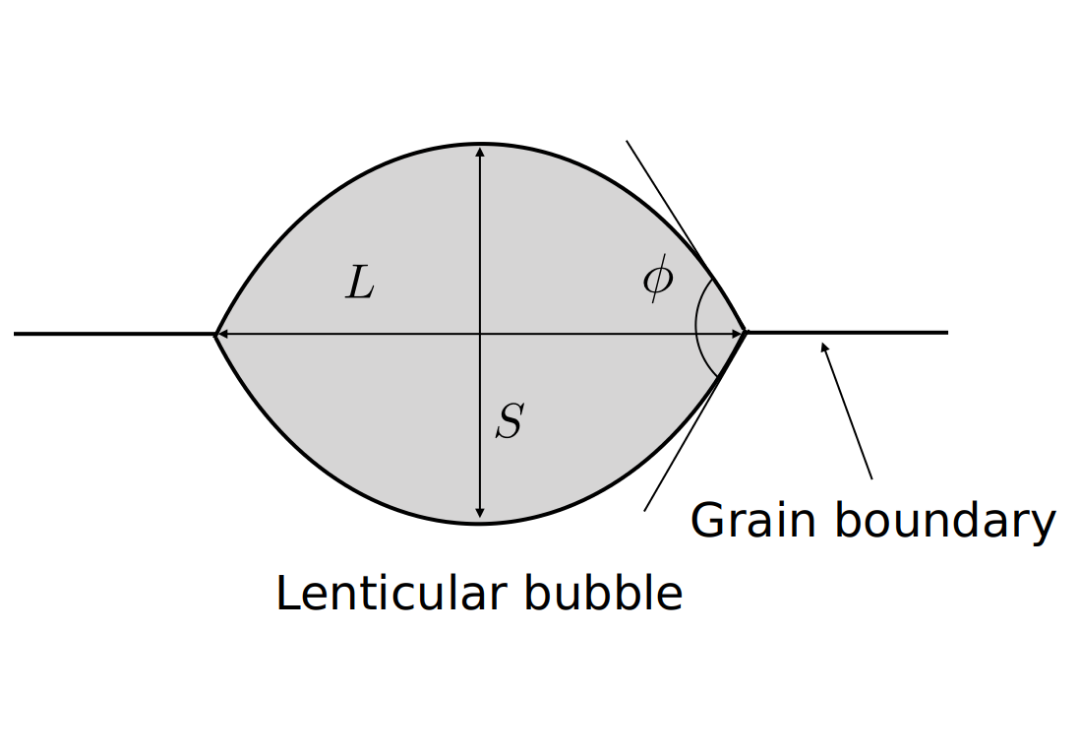
\includegraphics[width=\textwidth]{Chapter3/figures/bub}
        \caption{}
        \label{bubble_geo}
      \end{subfigure} \\
      \begin{subfigure}{0.4\textwidth}
        \centering
        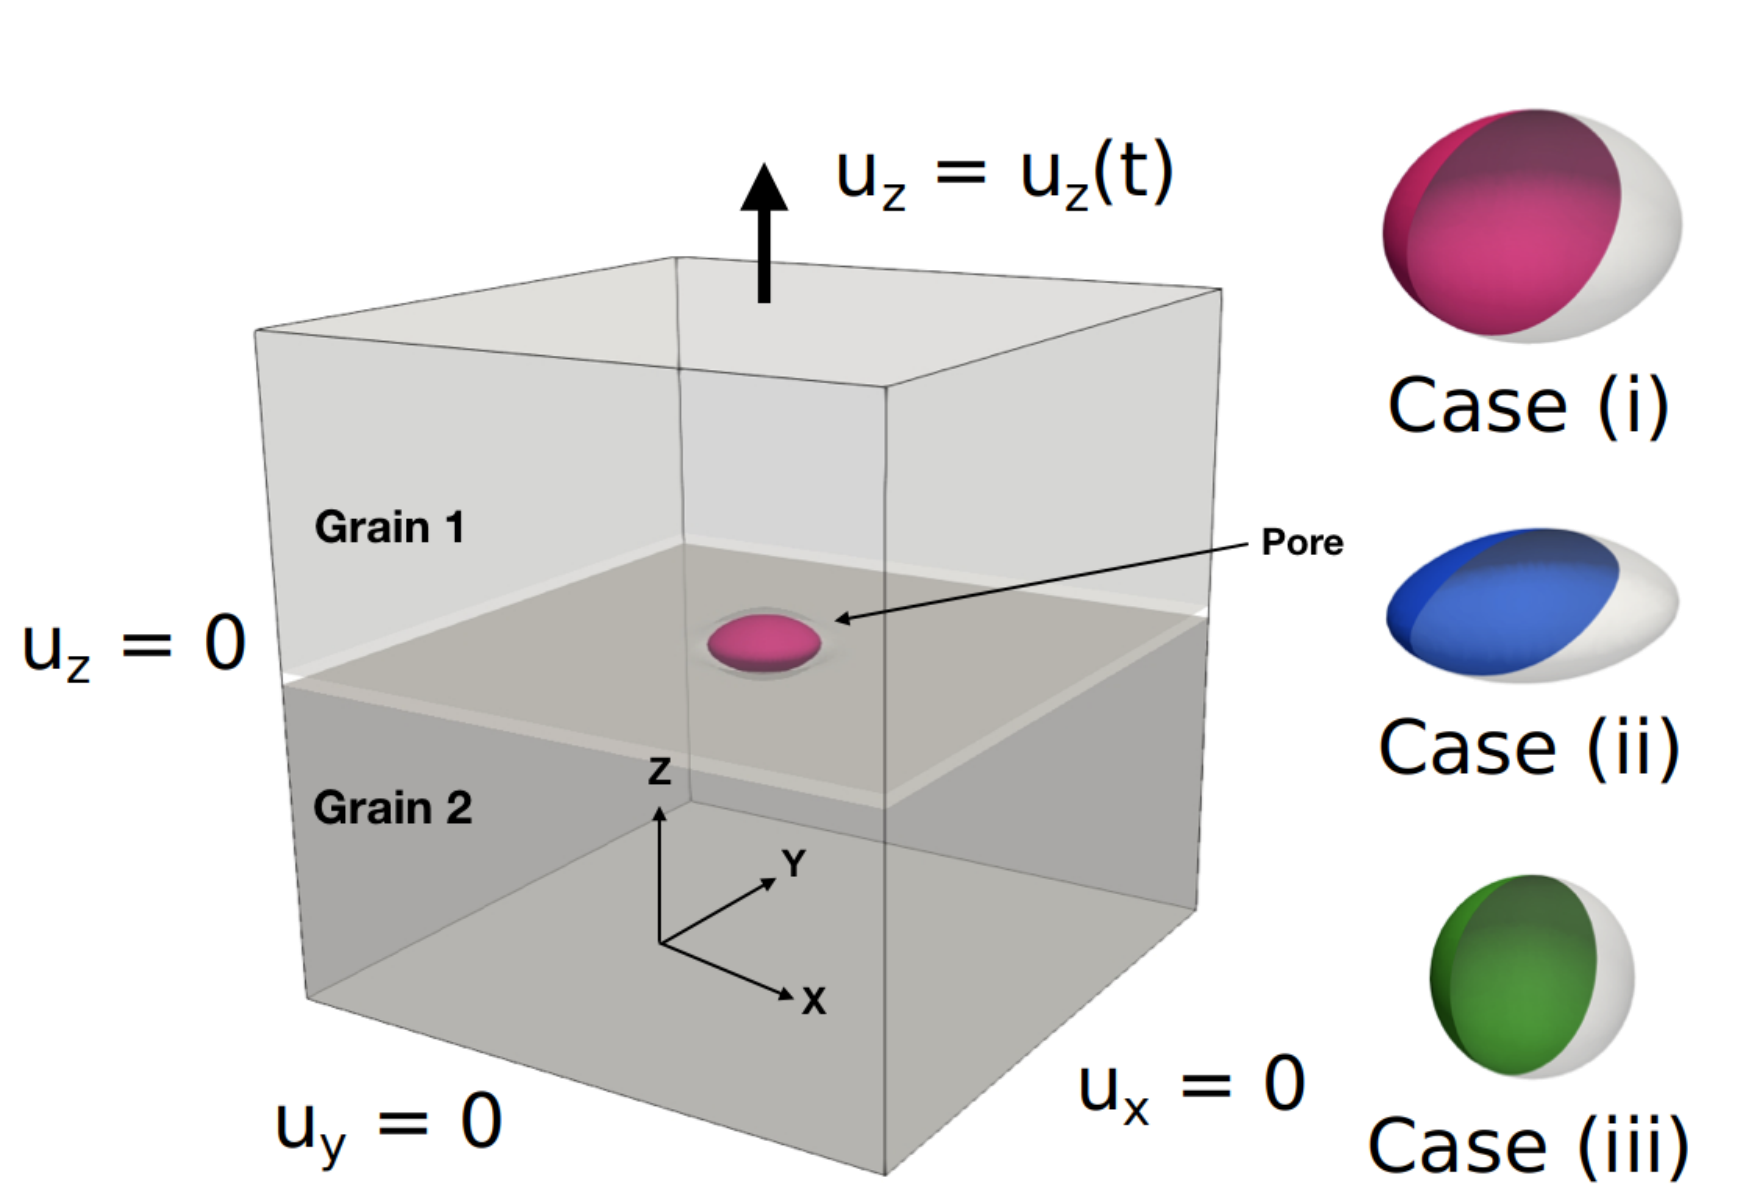
\includegraphics[width=\textwidth]{Chapter3/figures/single_ini}
        \caption{}
        \label{single_ini}
      \end{subfigure}
    \end{tabular}
     &                         
    \begin{subfigure}{0.4\textwidth}
      \centering
      \begin{tikzpicture}
        \begin{axis}[
            width=\textwidth,
            height=1.8\textwidth,
            xlabel=Strain,ylabel=Stress (MPa),
            xmin=0,
            xmax=0.006,
            ymin=0,
            ymax=1000,
            legend style={
                at={(0.02,0.98)},
                anchor=north west,
                nodes={scale=0.8, transform shape},
                text width=1.7in,
                minimum height=0.5in,
                draw=none,
                fill=none
              },
            legend cell align={left},
            every axis plot/.append style={line width=1pt}
          ]
          \addplot +[mark=none,color=black,solid] table[x expr=\thisrowno{2}/40,y=ave_stress_top] {Chapter3/data/single_case1.csv};
          \addplot +[mark=none,color=black,dashed] table[x expr=\thisrowno{2}/40,y=ave_stress_top] {Chapter3/data/single_case2.csv};
          \addplot +[mark=none,color=black,dotted] table[x expr=\thisrowno{2}/40,y=ave_stress_top] {Chapter3/data/single_case3.csv};
          \legend{case (i): Lenticular (large dihedral angle)),case (ii): Lenticular (small dihedral angle)),case (iii): Spherical}
        \end{axis}
      \end{tikzpicture}
      \caption{}
      \label{fig_bubble_geo_stress}
    \end{subfigure} \\
  \end{tabular}
  \caption[Comparison of stress-strain curves for different gas bubble geometries.]{ (a) The lenticular geometry is described by the length $L$, the thickness $S$ and the dihedral angle $\phi$. (b) Gas bubble geometry and boundary conditions. (c) Comparison of stress-strain curves for different gas bubble geometries.}
  \label{single_bub}
\end{figure}

%%%%%%%%%%%%%%%%%%%%%%%%%%%%%%%%%%%%%%%%%%%%%%%%%%%%%%%%%%%%%%%%%%%%%%%%%%%%%%%%%%%%%%%%%%%
%%%%%%%%%%%%%%%%%%%%%%%%%%%%%%%%%%%%%%%%%%%%%%%%%%%%%%%%%%%%%%%%%%%%%%%%%%%%%%%%%%%%%%%%%%%
%%%%%%%%%%%%%%%%%%%%%%%%%%%%%%%%%%%%%%%%%%%%%%%%%%%%%%%%%%%%%%%%%%%%%%%%%%%%%%%%%%%%%%%%%%%
%%%%%%%%%%%%%%%%%%%%%%%%%%%%%%%%%%%%%%%%%%%%%%%%%%%%%%%%%%%%%%%%%%%%%%%%%%%%%%%%%%%%%%%%%%%
%%%%%%%%%%%%%%%%%%%%%%%%%%%%%%%%%%%%%%%%%%%%%%%%%%%%%%%%%%%%%%%%%%%%%%%%%%%%%%%%%%%%%%%%%%%
%%%%%%%%%%%%%%%%%%%%%%%%%%%%%%%%%%%%%%%%%%%%%%%%%%%%%%%%%%%%%%%%%%%%%%%%%%%%%%%%%%%%%%%%%%%
%%%%%%%%%%%%%%%%%%%%%%%%%%%%%%%%%%%%%%%%%%%%%%%%%%%%%%%%%%%%%%%%%%%%%%%%%%%%%%%%%%%%%%%%%%%
%%%%%%%%%%%%%%%%%%%%%%%%%%%%%%%%%%%%%%%%%%%%%%%%%%%%%%%%%%%%%%%%%%%%%%%%%%%%%%%%%%%%%%%%%%%
%%%%%%%%%%%%%%%%%%%%%%%%%%%%%%%%%%%%%%%%%%%%%%%%%%%%%%%%%%%%%%%%%%%%%%%%%%%%%%%%%%%%%%%%%%%
%%%%%%%%%%%%%%%%%%%%%%%%%%%%%%%%%%%%%%%%%%%%%%%%%%%%%%%%%%%%%%%%%%%%%%%%%%%%%%%%%%%%%%%%%%%
\subsubsection{Effect of loading}

Next, we study the effect of different loading conditions. Uniaxial, biaxial and triaxial loading conditions are considered. The final crack configurations are shown in \Cref{final_loading}. A change in crack path due to a different loading condition is evident from the figure. For uniaxial loading, cracks propagate along the grain boundaries that are mainly perpendicular to the loading direction. For biaxial loading, crack branching occurs because biaxial loading results in two positive principal components of the strain tensor of the same order of magnitude. For triaxial loading, cracks propagate along all three directions.
\begin{figure}[!htb]
  \centering
  \begin{subfigure}{0.32\textwidth}
    \centering
    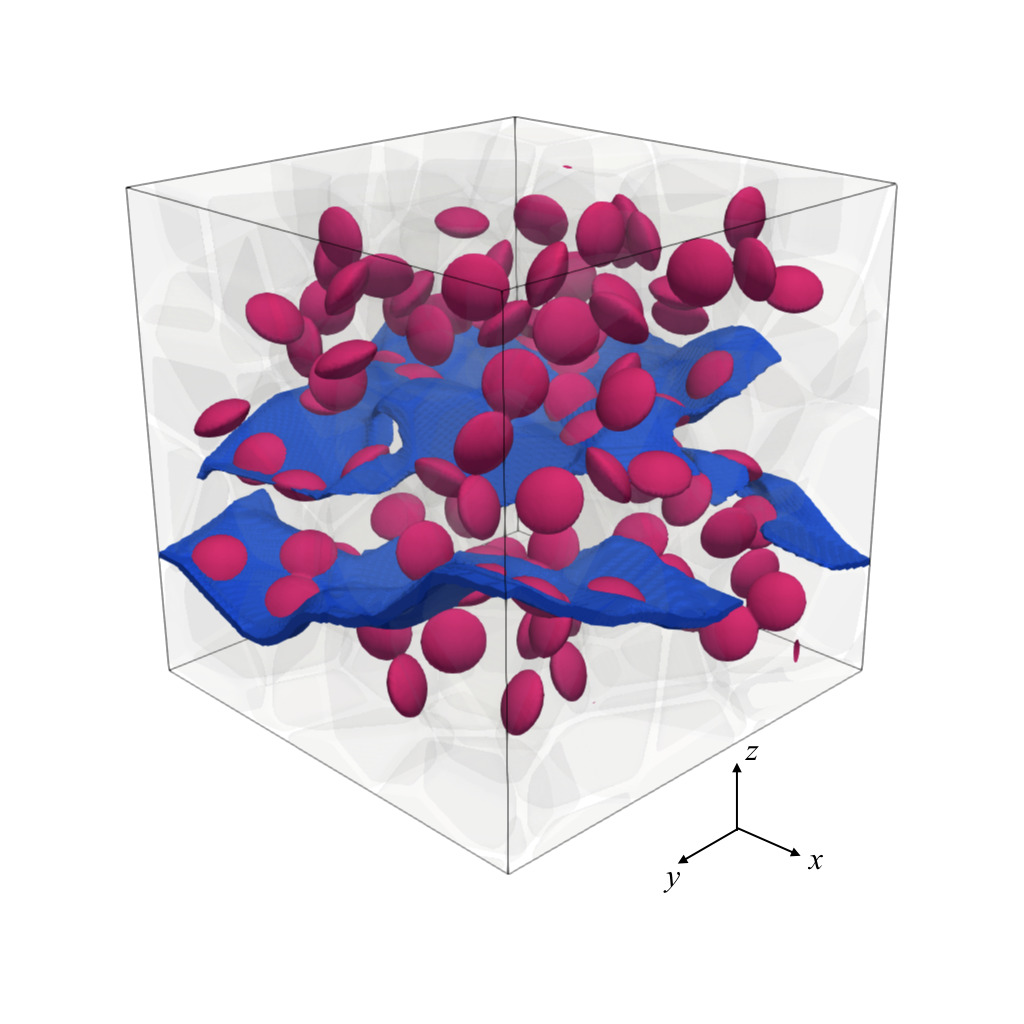
\includegraphics[width=\textwidth]{Chapter3/figures/b100_end}
    \caption{}
    \label{b100_load1}
  \end{subfigure}
  \begin{subfigure}{0.32\textwidth}
    \centering
    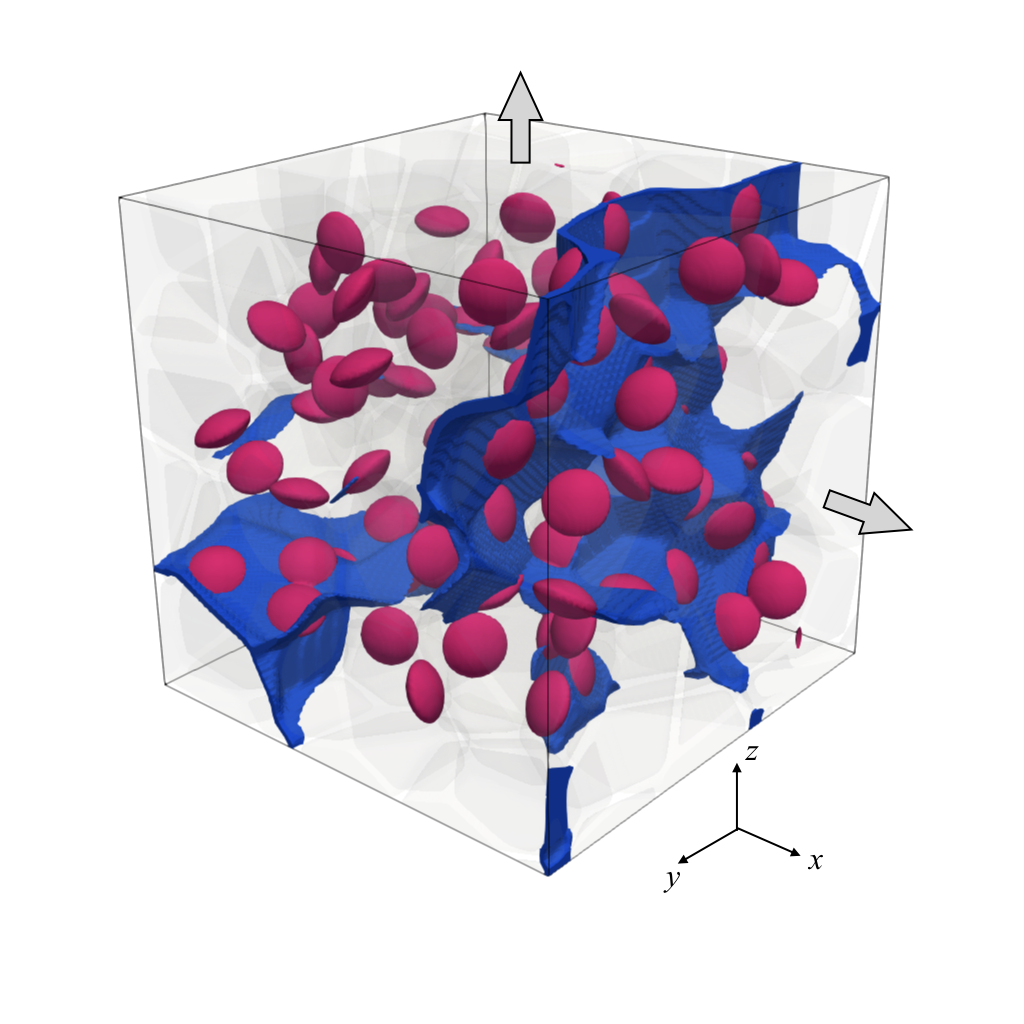
\includegraphics[width=\textwidth]{Chapter3/figures/b100_end_yz}
    \caption{}
    \label{b100_load2}
  \end{subfigure}
  \begin{subfigure}{0.32\textwidth}
    \centering
    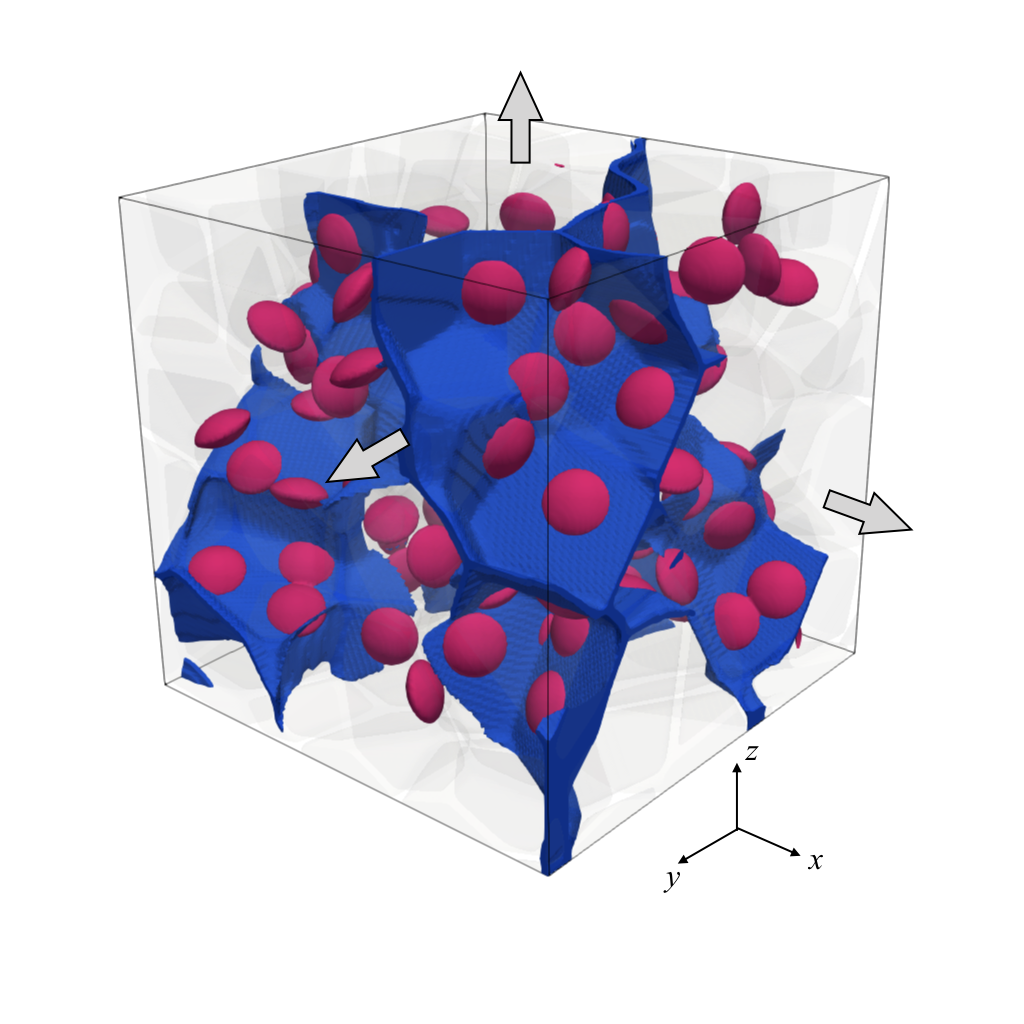
\includegraphics[width=\textwidth]{Chapter3/figures/b100_end_xyz}
    \caption{}
    \label{b100_load3}
  \end{subfigure}
  \caption{ Final configuration (crack surfaces highlighted in blue) for different loading (a) uniaxial (b) biaxial (c) triaxial.}
  \label{final_loading}
\end{figure}

The stress-strain curves are shown in \Cref{fig_loading}. The difference in the slopes during loading is due to the Poisson's effect. The sample under the biaxial and triaxial loading conditions manifests a lower critical fracture strength compared to that under uniaxial loading conditions. The critical strain corresponding to the critical fracture strength under triaxial loading is about half that under uniaxial loading.

\begin{figure}[!htb]
  \centering
  \begin{tikzpicture}
    \begin{axis}[
        width=0.8\textwidth,
        height=0.4\textwidth,
        xlabel=Strain,ylabel=Stress (MPa),
        xmin=0,
        xmax=0.0025,
        ymin=0,
        ymax=700,
        legend style={at={(0.05,0.95)},anchor=north west},
        legend style={nodes={scale=0.8, transform shape}},
        legend cell align={left},
        every axis plot/.append style={line width=1pt}
      ]
      \addplot +[mark=none,color=black,solid] table[x expr=\thisrowno{2}/40,y=ave_stress_top] {Chapter3/data/b100_y.csv};
      \addplot +[mark=none,color=black,dashed] table[x expr=\thisrowno{5}/40,y=ave_stress_top] {Chapter3/data/b100_yz.csv};
      \addplot +[mark=none,color=black,dotted] table[x expr=\thisrowno{5}/40,y=ave_stress_top] {Chapter3/data/b100_xyz.csv};
      \legend{Uniaxial loading,Biaxial loading,Triaxial loading}
    \end{axis}
  \end{tikzpicture}
  \caption{Comparison of stress-strain curves for different loading conditions.}
  \label{fig_loading}
\end{figure}

%%%%%%%%%%%%%%%%%%%%%%%%%%%%%%%%%%%%%%%%%%%%%%%%%%%%%%%%%%%%%%%%%%%%%%%%%%%%%%%%%%%%%%%%%%%
%%%%%%%%%%%%%%%%%%%%%%%%%%%%%%%%%%%%%%%%%%%%%%%%%%%%%%%%%%%%%%%%%%%%%%%%%%%%%%%%%%%%%%%%%%%
%%%%%%%%%%%%%%%%%%%%%%%%%%%%%%%%%%%%%%%%%%%%%%%%%%%%%%%%%%%%%%%%%%%%%%%%%%%%%%%%%%%%%%%%%%%
%%%%%%%%%%%%%%%%%%%%%%%%%%%%%%%%%%%%%%%%%%%%%%%%%%%%%%%%%%%%%%%%%%%%%%%%%%%%%%%%%%%%%%%%%%%
%%%%%%%%%%%%%%%%%%%%%%%%%%%%%%%%%%%%%%%%%%%%%%%%%%%%%%%%%%%%%%%%%%%%%%%%%%%%%%%%%%%%%%%%%%%
%%%%%%%%%%%%%%%%%%%%%%%%%%%%%%%%%%%%%%%%%%%%%%%%%%%%%%%%%%%%%%%%%%%%%%%%%%%%%%%%%%%%%%%%%%%
%%%%%%%%%%%%%%%%%%%%%%%%%%%%%%%%%%%%%%%%%%%%%%%%%%%%%%%%%%%%%%%%%%%%%%%%%%%%%%%%%%%%%%%%%%%
%%%%%%%%%%%%%%%%%%%%%%%%%%%%%%%%%%%%%%%%%%%%%%%%%%%%%%%%%%%%%%%%%%%%%%%%%%%%%%%%%%%%%%%%%%%
%%%%%%%%%%%%%%%%%%%%%%%%%%%%%%%%%%%%%%%%%%%%%%%%%%%%%%%%%%%%%%%%%%%%%%%%%%%%%%%%%%%%%%%%%%%
%%%%%%%%%%%%%%%%%%%%%%%%%%%%%%%%%%%%%%%%%%%%%%%%%%%%%%%%%%%%%%%%%%%%%%%%%%%%%%%%%%%%%%%%%%%
\subsubsection{Effect of porosity}

In 2D, under plane-strain assumptions, the porosity represented by a planar bubble is computed by extruding it along the out-of-plane direction, which overestimates the actual porosity. In order to obtain a reasonable correlation between the critical fracture strength and the porosity, a 3D model is necessary.

To study the effect of porosity, consider an REV with side length of \SI{40}{\micro\meter}. Grain centroids are generated from a random close-packing (RCP) voronoi structure. The RCP structures can be realized by a spatial sampling process known as Maximal Poisson-disk Sampling (MPS) \cite{Ebeida2012}. For the RCP voronoi structure, the average aspect ratio of each voronoi cell is approximately 1 and an equiaxed grain structure is provided.

The influence of the voronoi structure on fracture properties can be isolated by considering a specific realization of RCP. The realization under consideration consists of 77 grains and the average radius of grains is \SI{9.4}{\micro\meter}. As shown in \Cref{ini_final_porosity}, 50, 100 and 150 gas bubbles are randomly distributed over the grain boundaries, with corresponding porosity values $2.02\%$, $4.04\%$ and $6.06\%$, respectively. All gas bubbles have a lenticular shape with $L = \SI{6.4}{\micro\meter}$, $S = \SI{4}{\micro\meter}$, and $\phi=\SI{128}{\degree}$. Symmetric boundary conditions are prescribed and a uniform displacement is applied on the top of the REV.

Final configurations of the approximated crack surfaces are shown in \Cref{ini_final_porosity}, where, in general, cracks propagate perpendicular to the direction of the applied load.
It is worth noting that cracks keep propagating after initiation without any increase in the applied stress, which suggests that a snap-back is likely to take place after crack initiation and a mixed force-displacement control is necessary to follow the actual stress-strain curve without loss of information. However, we argue that the simple displacement control suffices to obtain the critical fracture strength -- the maximum stress value along the stress-strain curve. From \Cref{fig_porosity}, we conclude that an increase in porosity leads to a higher probability of crack initiation at a lower stress state and consequently a decrease in the critical fracture strength.
\begin{figure}[!htb]
  \centering
  \begin{subfigure}{0.32\textwidth}
    \centering
    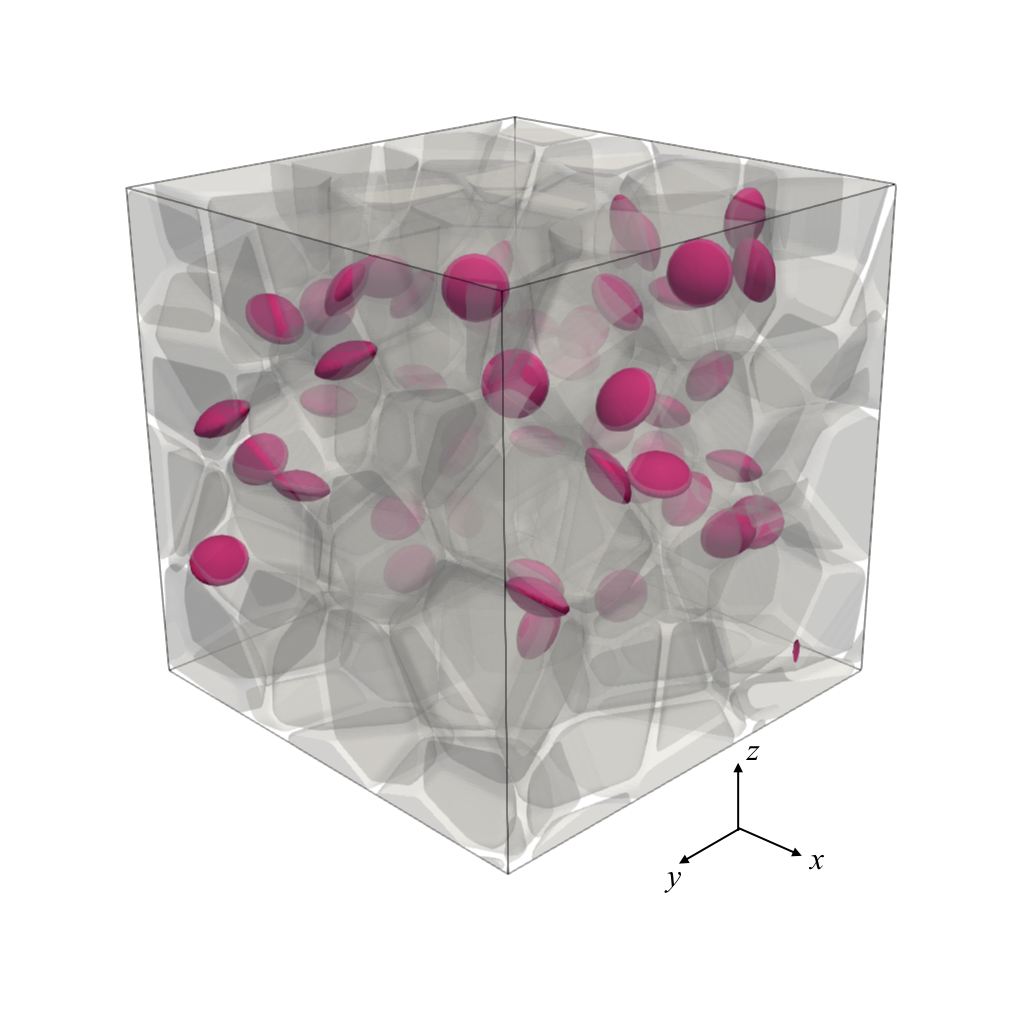
\includegraphics[width=\textwidth]{Chapter3/figures/b50_ini_new}
    \caption{}
    \label{b50_ini}
  \end{subfigure}
  \begin{subfigure}{0.32\textwidth}
    \centering
    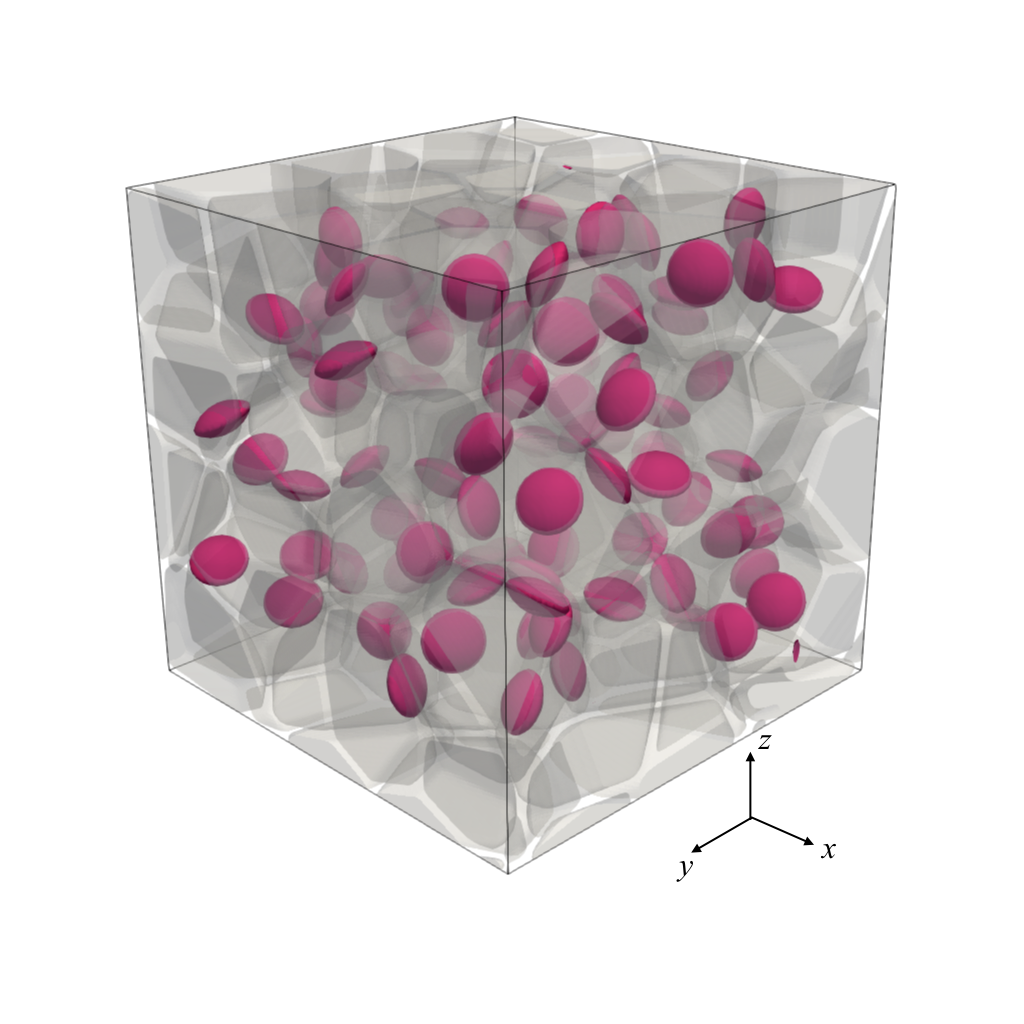
\includegraphics[width=\textwidth]{Chapter3/figures/b100_ini_new}
    \caption{}
    \label{b100_ini}
  \end{subfigure}
  \begin{subfigure}{0.32\textwidth}
    \centering
    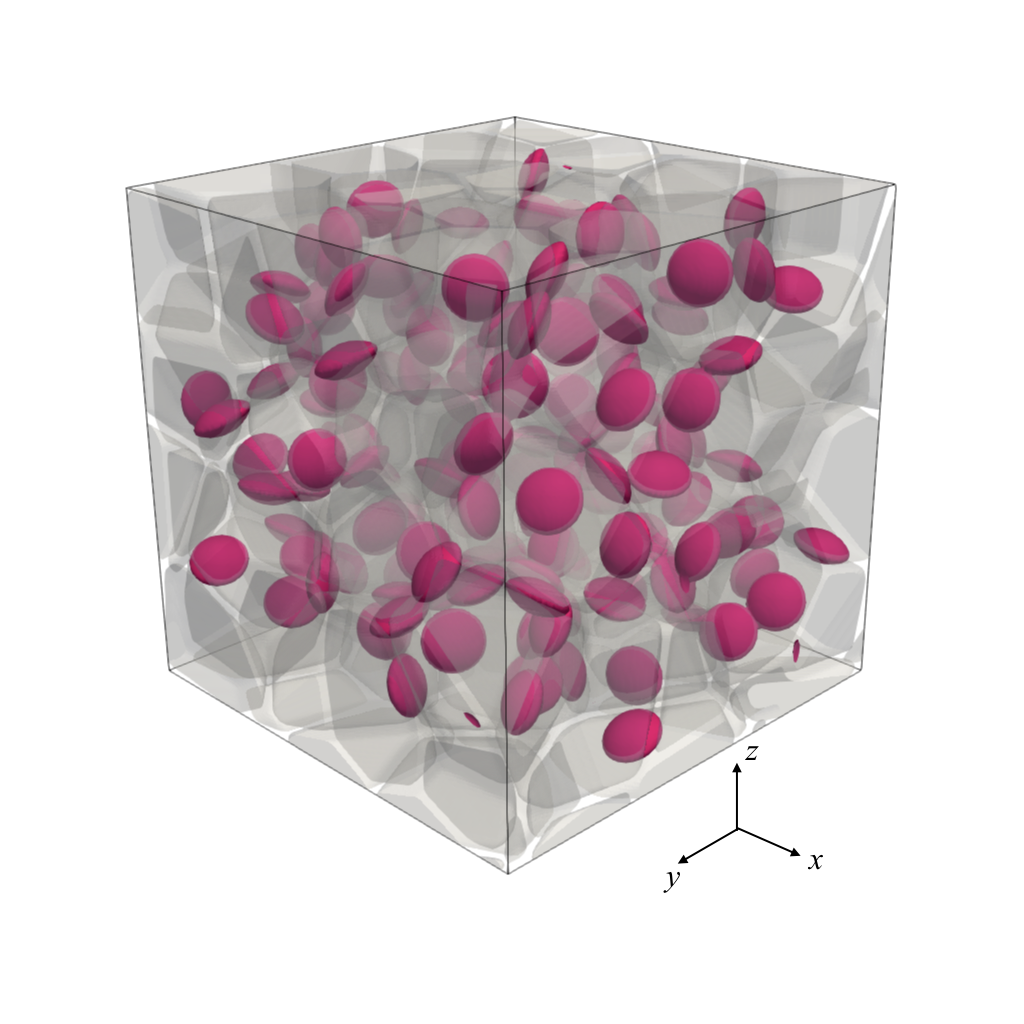
\includegraphics[width=\textwidth]{Chapter3/figures/b150_ini_new}
    \caption{}
    \label{b150_ini}
  \end{subfigure}
  \begin{subfigure}{0.32\textwidth}
    \centering
    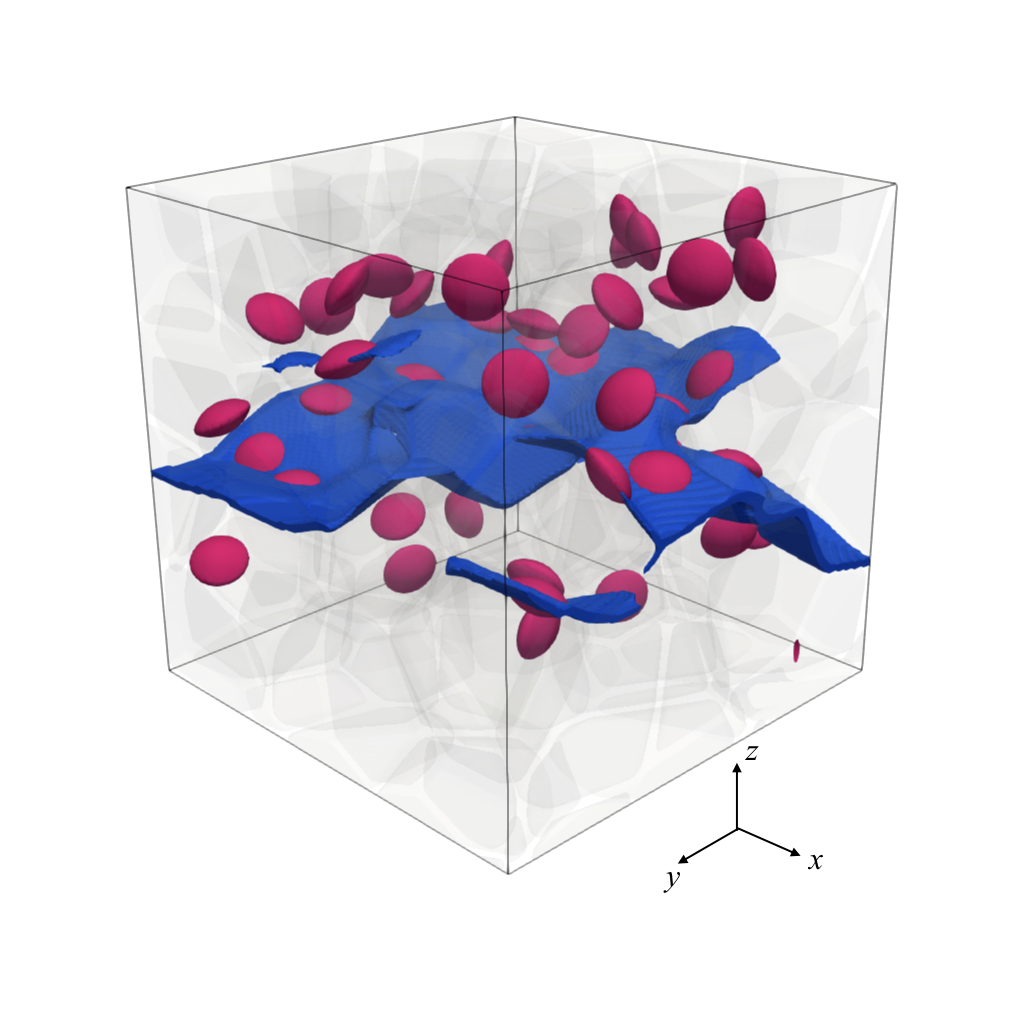
\includegraphics[width=\textwidth]{Chapter3/figures/b50_end}
    \caption{}
    \label{b50_end}
  \end{subfigure}
  \begin{subfigure}{0.32\textwidth}
    \centering
    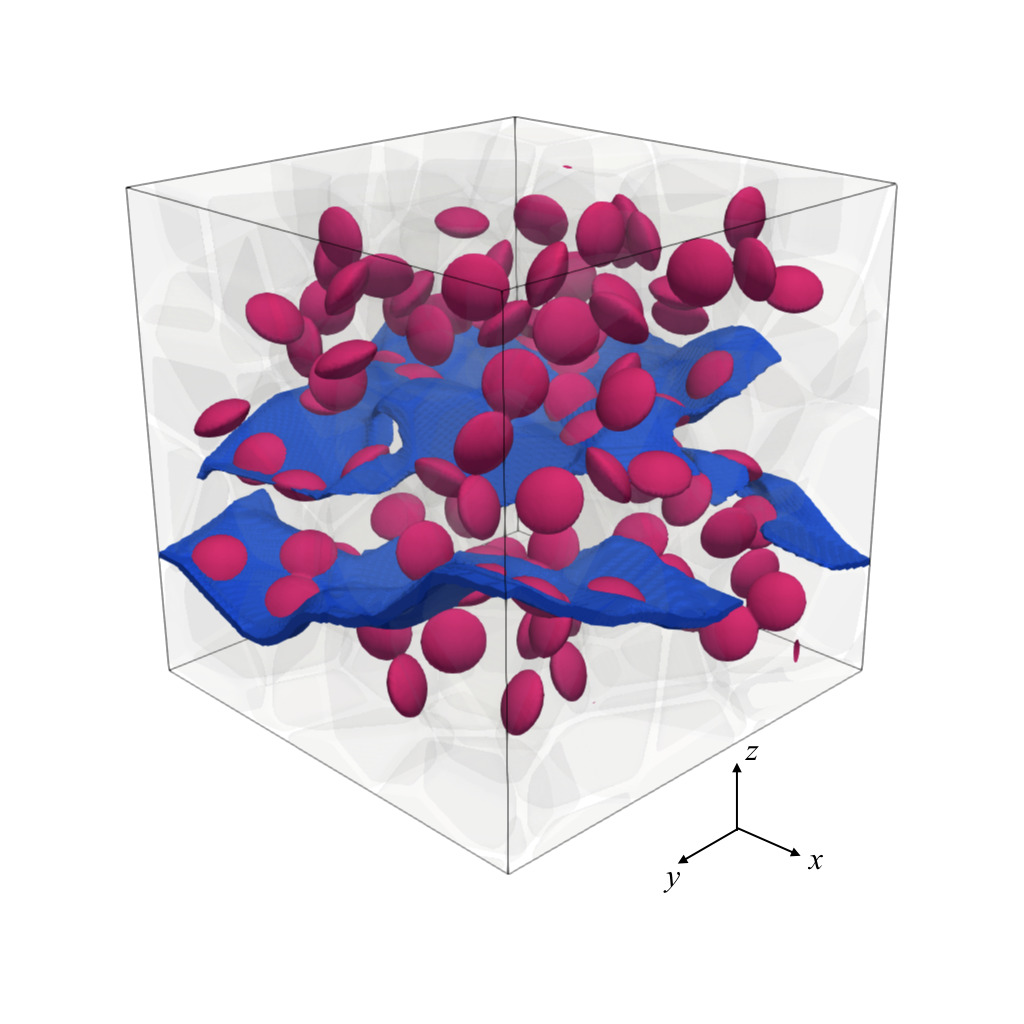
\includegraphics[width=\textwidth]{Chapter3/figures/b100_end}
    \caption{}
    \label{b100_end}
  \end{subfigure}
  \begin{subfigure}{0.32\textwidth}
    \centering
    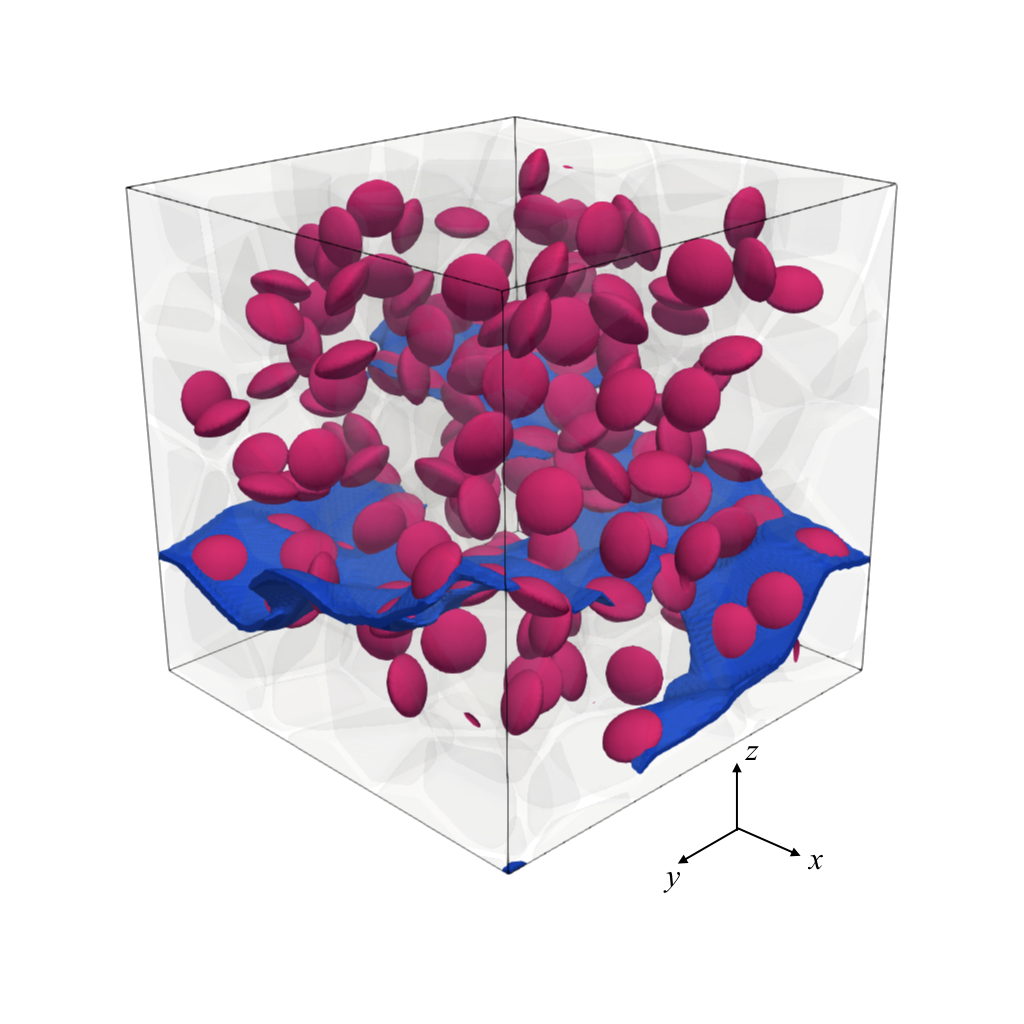
\includegraphics[width=\textwidth]{Chapter3/figures/b150_end}
    \caption{}
    \label{b150_end}
  \end{subfigure}
  \caption[Crack propagation in REVs with different porosity values.]{ (a-c) Initial configuration of REVs with an average grain size of \SI{9.4}{\micro\meter}. (d-f) Final configuration (crack surfaces highlighted in blue) for REVs. Different porosity values are considered: (a, d) $2.02\%$, (b, e) $4.04\%$, (c, f) $6.06\%$. }
  \label{ini_final_porosity}
\end{figure}

\begin{figure}[!htb]
  \centering
  \begin{tikzpicture}
    \begin{axis}[
        width=0.8\textwidth,
        height=0.4\textwidth,
        xlabel=Strain,ylabel=Stress (MPa),
        xmin=0,
        xmax=0.0025,
        ymin=0,
        ymax=700,
        legend style={
            at={(0.02,0.98)},
            anchor=north west,
            nodes={scale=0.8, transform shape},
            draw=none,
            fill=none
          },
        legend cell align={left},
        every axis plot/.append style={line width=1pt}
      ]
      \addplot +[mark=none,color=black,solid] table[x expr=\thisrowno{2}/40,y=ave_stress_top] {Chapter3/data/b50_out.csv};
      \addplot +[mark=none,color=black,dashed] table[x expr=\thisrowno{2}/40,y=ave_stress_top] {Chapter3/data/b100_out.csv};
      \addplot +[mark=none,color=black,dotted] table[x expr=\thisrowno{2}/40,y=ave_stress_top] {Chapter3/data/b150_out.csv};
      \legend{Porosity 2.02\% (50 bubbles),Porosity 4.04\% (100 bubbles),Porosity 6.06\% (150 bubbles)}
    \end{axis}
  \end{tikzpicture}
  \caption{Comparison of stress-strain curves for different porosity values.}
  \label{fig_porosity}
\end{figure}

To describe the porosity, average gas bubble and grain size effect on fracture strength, an exponential functional form obtained from a biaxial flexure test has been reported in \cite{oguma_1982}:
\begin{align}
  \dfrac{\sigma_c}{\sigma_0} = \exp(-a r),
\end{align}
where $r$ is the porosity. The critical fracture strength is normalized with respect to $\sigma_0$. To benchmark with experiments, $\sigma_0$ is obtained by substituting the average grain and bubble size of \SI{9.4}{\micro\meter} and \SI{5.2}{\micro\meter}. To give proper error bounds on our numerical predictions, five trial calculations were performed on five different realizations of the spatial distribution of bubbles for each porosity level. The fracture strength values obtained from 15 realizations of 3 porosity levels are summarized in \Cref{fs15}. The fitted $\sigma_0$ is \SI{198}{\mega\pascal}, \SI{693}{\mega\pascal} and \SI{697.8}{\mega\pascal} and the coefficient $a$ is 0.057, 0.14 and 0.04, for experiment, 2D simulations and 3D simulations, respectively.
A comparison of the experimental model, previous 2D simulations \cite{pritam_2016} and current 3D simulations is shown in \Cref{fig_rfit_porosity}. In particular, the $95\%$ confidence interval for the 3D simulations is shown in stripes. It shows that the 3D simulation has significant improvement towards the prediction of the dependence of the critical fracture strength on porosity. It is worth mentioning that the difference between simulation predictions of $\sigma_0$ and experimental values could be due to the fact that the transgranular fracture observed in experiments \cite{evans_1969} has not been incorporated into the current numerical model.

\begin{table}[!htb]
  \centering
  \caption{Summary of fracture strength obtained from 15 realizations of 3 porosity values. R denotes the realization index.}
  \begin{tabular}{*6c}
    \toprule
    Porosity (\%) & \multicolumn{5}{c}{Critical fracture strength (\SI{}{\mega\pascal})}                                 \\
    \midrule
                  & R1                                                                   & R2    & R3    & R4    & R5    \\
    \midrule
    2.02          & 631.4                                                                & 657.4 & 645.6 & 663.4 & 630.7 \\
    4.04          & 609.8                                                                & 555.6 & 605.5 & 611.2 & 589.2 \\
    6.06          & 540.0                                                                & 530.8 & 557.0 & 563.2 & 567.9 \\
    \bottomrule
  \end{tabular}
  \label{fs15}
\end{table}

\begin{figure}[!htb]
  \centering
  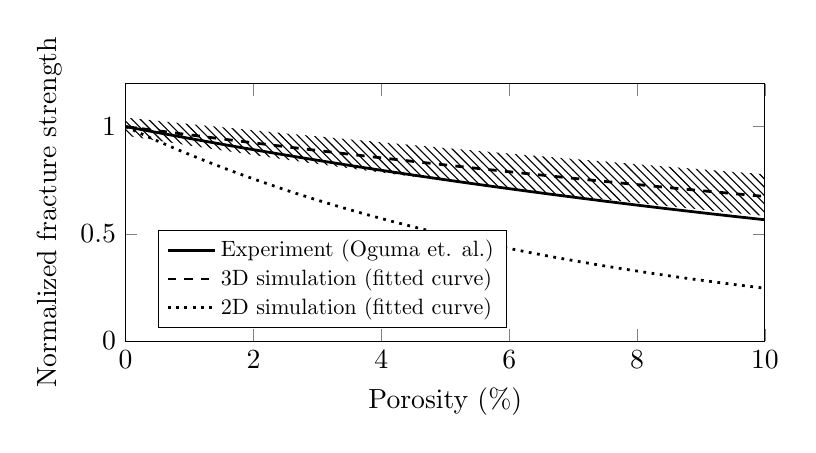
\begin{tikzpicture}
    \begin{axis}[
        width=0.8\textwidth,
        height=0.4\textwidth,
        xlabel=Porosity (\%),ylabel=Normalized fracture strength,
        xmin=0,
        xmax=10,
        ymin=0,
        ymax=1.2,
        legend style={at={(0.05,0.05)},anchor=south west},
        legend style={nodes={scale=0.8, transform shape}},
        legend cell align={left},
        every axis plot/.append style={line width=1pt}
      ]
      % plot the confidence interval band
      \addplot [name path=upper,draw=none,domain=0:10,forget plot] {727/697.8*exp(-0.02925*x)};
      \addplot [name path=lower,draw=none,domain=0:10,forget plot] {668.5/697.8*exp(-0.04959*x)};
      \tikzfillbetween[of=upper and lower]{pattern=north west lines};
      % experiment
      \addplot +[mark=none,color=black,solid,domain=0:10] {exp(-0.057*x)};
      % 3D
      \addplot +[mark=none,color=black,dashed,domain=0:10] {exp(-0.03942*x)};
      % 2D
      \addplot +[mark=none,color=black,dotted,domain=0:10] {exp(-0.14*x)};
      \legend{Experiment (Oguma et. al.),3D simulation (fitted curve), 2D simulation (fitted curve)}
    \end{axis}
  \end{tikzpicture}
  \caption[Variation in normalized fracture strength with changing porosity.]{Variation in normalized fracture strength with changing porosity. Five trial calculations were performed for each porosity level, and each calculation was based on one realization of the spatial distribution of bubbles. The 95\% confidence interval is shown in stripes.}
  \label{fig_rfit_porosity}
\end{figure}

%%%%%%%%%%%%%%%%%%%%%%%%%%%%%%%%%%%%%%%%%%%%%%%%%%%%%%%%%%%%%%%%%%%%%%%%%%%%%%%%%%%%%%%%%%%
%%%%%%%%%%%%%%%%%%%%%%%%%%%%%%%%%%%%%%%%%%%%%%%%%%%%%%%%%%%%%%%%%%%%%%%%%%%%%%%%%%%%%%%%%%%
%%%%%%%%%%%%%%%%%%%%%%%%%%%%%%%%%%%%%%%%%%%%%%%%%%%%%%%%%%%%%%%%%%%%%%%%%%%%%%%%%%%%%%%%%%%
%%%%%%%%%%%%%%%%%%%%%%%%%%%%%%%%%%%%%%%%%%%%%%%%%%%%%%%%%%%%%%%%%%%%%%%%%%%%%%%%%%%%%%%%%%%
%%%%%%%%%%%%%%%%%%%%%%%%%%%%%%%%%%%%%%%%%%%%%%%%%%%%%%%%%%%%%%%%%%%%%%%%%%%%%%%%%%%%%%%%%%%
%%%%%%%%%%%%%%%%%%%%%%%%%%%%%%%%%%%%%%%%%%%%%%%%%%%%%%%%%%%%%%%%%%%%%%%%%%%%%%%%%%%%%%%%%%%
%%%%%%%%%%%%%%%%%%%%%%%%%%%%%%%%%%%%%%%%%%%%%%%%%%%%%%%%%%%%%%%%%%%%%%%%%%%%%%%%%%%%%%%%%%%
%%%%%%%%%%%%%%%%%%%%%%%%%%%%%%%%%%%%%%%%%%%%%%%%%%%%%%%%%%%%%%%%%%%%%%%%%%%%%%%%%%%%%%%%%%%
%%%%%%%%%%%%%%%%%%%%%%%%%%%%%%%%%%%%%%%%%%%%%%%%%%%%%%%%%%%%%%%%%%%%%%%%%%%%%%%%%%%%%%%%%%%
%%%%%%%%%%%%%%%%%%%%%%%%%%%%%%%%%%%%%%%%%%%%%%%%%%%%%%%%%%%%%%%%%%%%%%%%%%%%%%%%%%%%%%%%%%%
\subsection{High burnup structure fragmentation}

Next, we adopt the quasi-brittle fracture model to simulate fission-gas-induced intergranular fracture of UO$_2$ HBS. A two-dimensional REV with side length $L = \SI{3}{\micro\meter}$ is considered, and plane-strain conditions are assumed to hold. The material properties and model parameters are summarized in \Cref{table: HBS material properties}. The critical fracture energy of UO$_2$ is taken to be \SI{0.022}{\milli\joule\per\cubic\milli\meter} \cite{oguma_1982}.
Due to the lack of experimental data, the fracture toughness $\Gc^g$ is assumed to be \SI{1.2e-6}{\milli\joule\per\cubic\milli\meter} and the characteristic length $l_\text{ch} = \dfrac{\Gc}{2\psi_c} \approx \SI{22.78}{\nano\meter}$. The domain is uniformly discretized with \texttt{QUAD4} elements with element size of $\SI{0.005}{\micro\meter}$.

\begin{table}[!htb]
  \centering
  \caption{Parameters and material properties used in the fission-gas-induced HBS fracture simulations.}
  \label{table: HBS material properties}
  \begin{tabular}{ r c c c c }
    \toprule
    \textbf{Property}                 & \textbf{Symbol} & \textbf{Value} & \textbf{Unit}                             & \textbf{Reference} \\
    \midrule
    Young's modulus                   & $E$             & 385            & \SI{}{\giga\pascal}                       & \cite{govers_2007} \\
    Critical fracture energy          & $\psi_c$        & 0.022          & \SI{}{\milli\joule\per\cubic\milli\meter} & \cite{oguma_1982}  \\
    Grain boundary fracture toughness & $\Gc^g$         & \SI{1.2e-6}{}  & \SI{}{\milli\joule\per\cubic\milli\meter} &                    \\
    Grain fracture toughness          & $\Gc^b$         & \SI{1.2e-5}{}  & \SI{}{\milli\joule\per\cubic\milli\meter} &                    \\
    Phase-field regularization length & $l$             & 0.01           & \SI{}{\micro\meter}                       &                    \\
    \bottomrule
  \end{tabular}
\end{table}

%%%%%%%%%%%%%%%%%%%%%%%%%%%%%%%%%%%%%%%%%%%%%%%%%%%%%%%%%%%%%%%%%%%%%%%%%%%%%%%%%%%%%%%%%%%
%%%%%%%%%%%%%%%%%%%%%%%%%%%%%%%%%%%%%%%%%%%%%%%%%%%%%%%%%%%%%%%%%%%%%%%%%%%%%%%%%%%%%%%%%%%
%%%%%%%%%%%%%%%%%%%%%%%%%%%%%%%%%%%%%%%%%%%%%%%%%%%%%%%%%%%%%%%%%%%%%%%%%%%%%%%%%%%%%%%%%%%
%%%%%%%%%%%%%%%%%%%%%%%%%%%%%%%%%%%%%%%%%%%%%%%%%%%%%%%%%%%%%%%%%%%%%%%%%%%%%%%%%%%%%%%%%%%
%%%%%%%%%%%%%%%%%%%%%%%%%%%%%%%%%%%%%%%%%%%%%%%%%%%%%%%%%%%%%%%%%%%%%%%%%%%%%%%%%%%%%%%%%%%
%%%%%%%%%%%%%%%%%%%%%%%%%%%%%%%%%%%%%%%%%%%%%%%%%%%%%%%%%%%%%%%%%%%%%%%%%%%%%%%%%%%%%%%%%%%
%%%%%%%%%%%%%%%%%%%%%%%%%%%%%%%%%%%%%%%%%%%%%%%%%%%%%%%%%%%%%%%%%%%%%%%%%%%%%%%%%%%%%%%%%%%
%%%%%%%%%%%%%%%%%%%%%%%%%%%%%%%%%%%%%%%%%%%%%%%%%%%%%%%%%%%%%%%%%%%%%%%%%%%%%%%%%%%%%%%%%%%
%%%%%%%%%%%%%%%%%%%%%%%%%%%%%%%%%%%%%%%%%%%%%%%%%%%%%%%%%%%%%%%%%%%%%%%%%%%%%%%%%%%%%%%%%%%
%%%%%%%%%%%%%%%%%%%%%%%%%%%%%%%%%%%%%%%%%%%%%%%%%%%%%%%%%%%%%%%%%%%%%%%%%%%%%%%%%%%%%%%%%%%
\subsubsection{LOCA pressure transients}

We begin by investigating gas-pressure-induced fracture during LOCA-driven temperature transients. During a LOCA transient, temperatures in the fuel rod increase rapidly, leading to increased pressure in the gas contained within the bubbles. The temperature as a function of time at the edge of a representative pellet for each rod is obtained from simulation of the Studsvik Rod 196 experiment \cite{STUDSVIK} using the engineering-scale fuel performance code BISON \cite{WILLIAMSON2020}. The temperature transient is used as an input to the Kim-Kim-Suzuki (KKS) phase-field model \cite{Aagesen2020} to determine the pressure as a function of time. In the KKS model, the gas pressure is assumed to be \SI{100}{\mega\pascal} during steady-state reactor operation at \SI{700}{\kelvin}. The Studsvik experiment is initialized with a fixed temperature $T = \SI{572.6}{\kelvin}$ at the outer surface prior to the transient, resulting in a decrease in the pressure from \SI{100}{\mega\pascal} to below \SI{80}{\mega\pascal}. The pressure is assumed to be known in the quasi-brittle fracture model to simulate crack nucleation and propagation in the surrounding regions of the individual bubbles.

Two bubble radii (\SI{0.25}{\micro\meter} and \SI{0.5}{\micro\meter}) are considered, and no loading is applied on the exterior. The resulting fracture patterns are shown in \Cref{fig:r25}. With the smaller bubble, two cracks propagate from the bubble towards the outer surface. With a larger bubble, only one major crack propagates to the free surface, and other minor cracks are arrested. Cracks nucleate when the tensile stress on the bubble-matrix interface reaches the critical fracture strength. The critical pressures are \SI{120.17}{\mega\pascal} and \SI{89.69}{\mega\pascal} for the small and large bubbles, respectively. The critical pressure is significantly lower for the larger bubble.

\begin{figure}[htb!]
  \centering
  \begin{subfigure}[t]{0.32\linewidth}
    \centering
    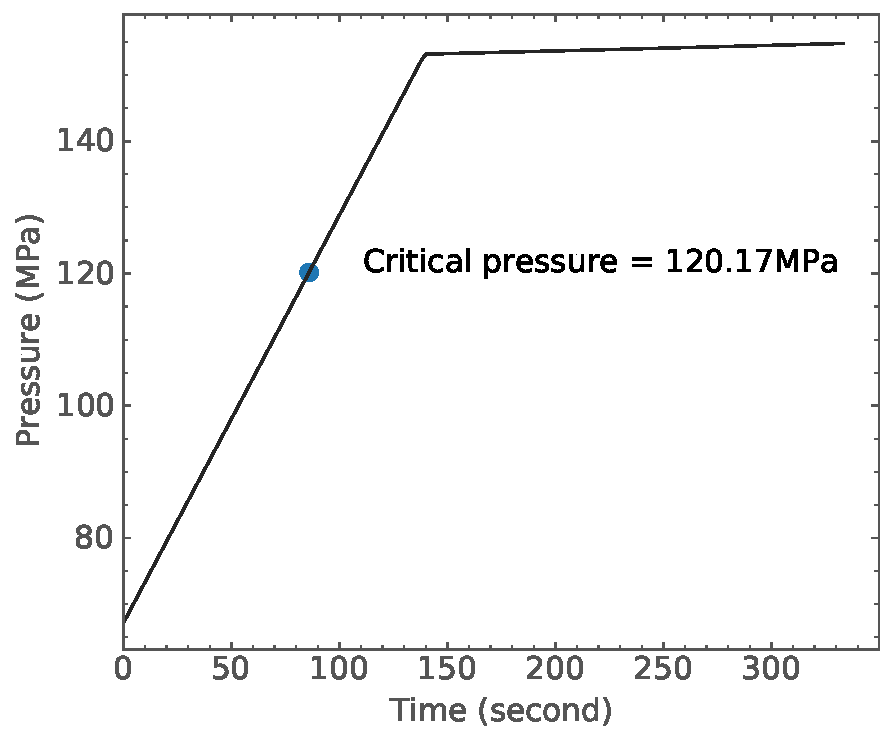
\includegraphics[width=\linewidth]{Chapter3/figures/bubble_pressure_r0.25_ext0_rod196}
    \caption{}
  \end{subfigure}
  \begin{subfigure}[t]{0.32\linewidth}
    \centering
    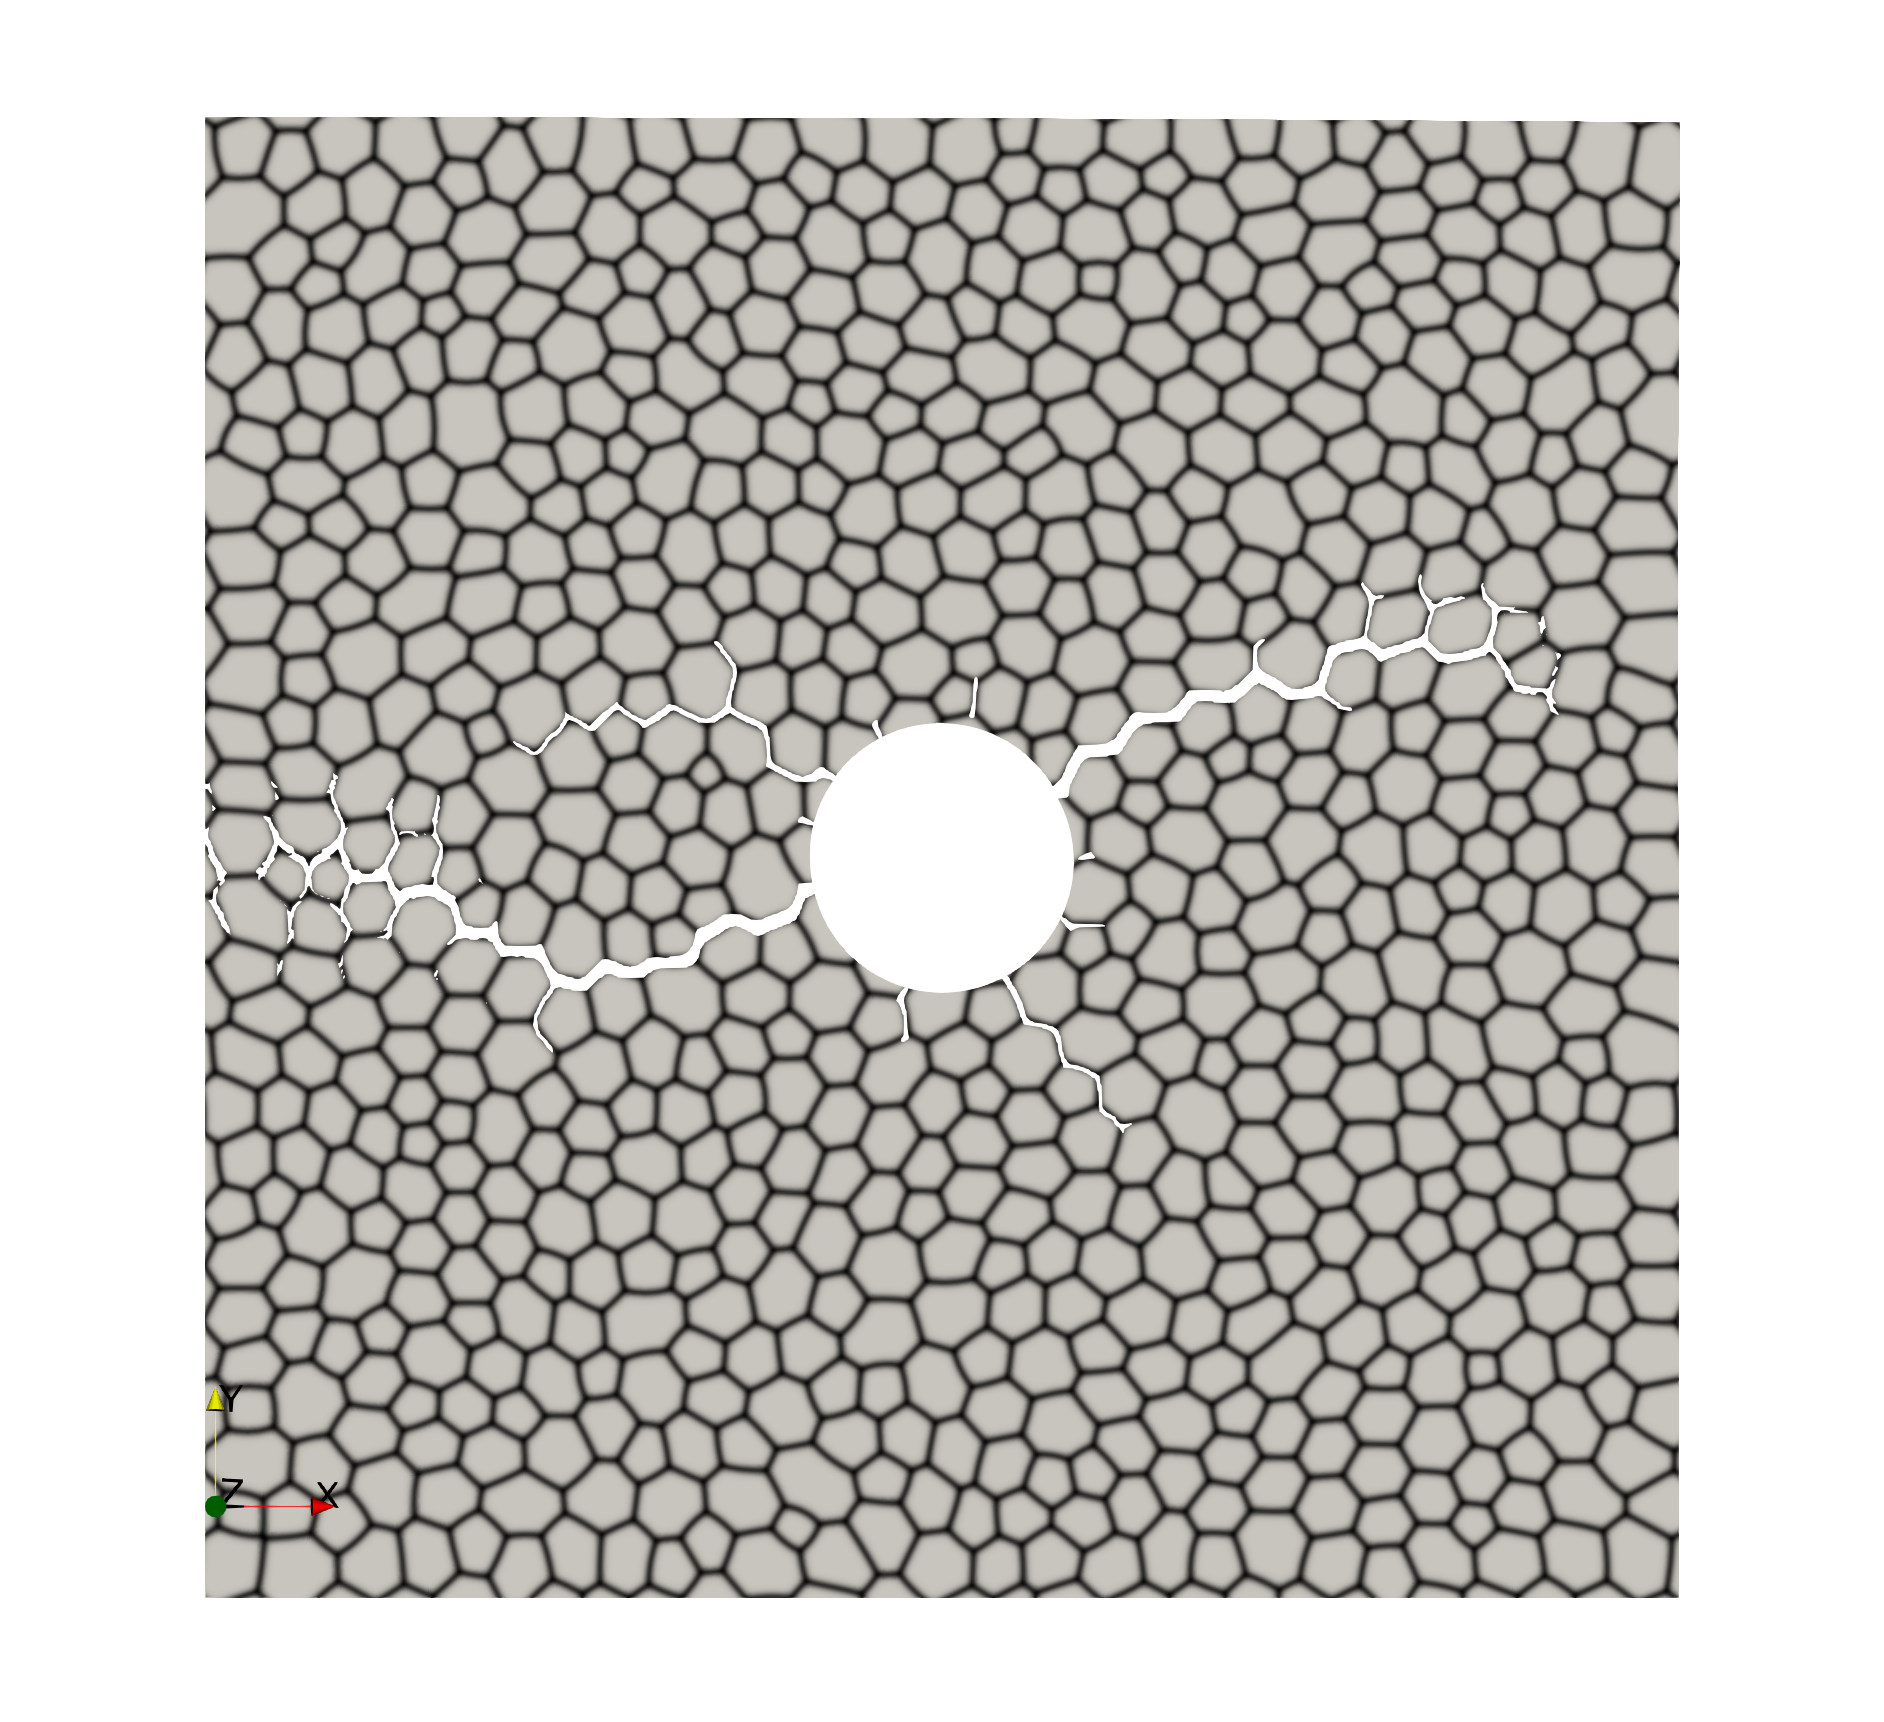
\includegraphics[width=\linewidth]{Chapter3/figures/r25_ext0}
    \caption{}
  \end{subfigure}
  \begin{subfigure}[t]{0.32\linewidth}
    \centering
    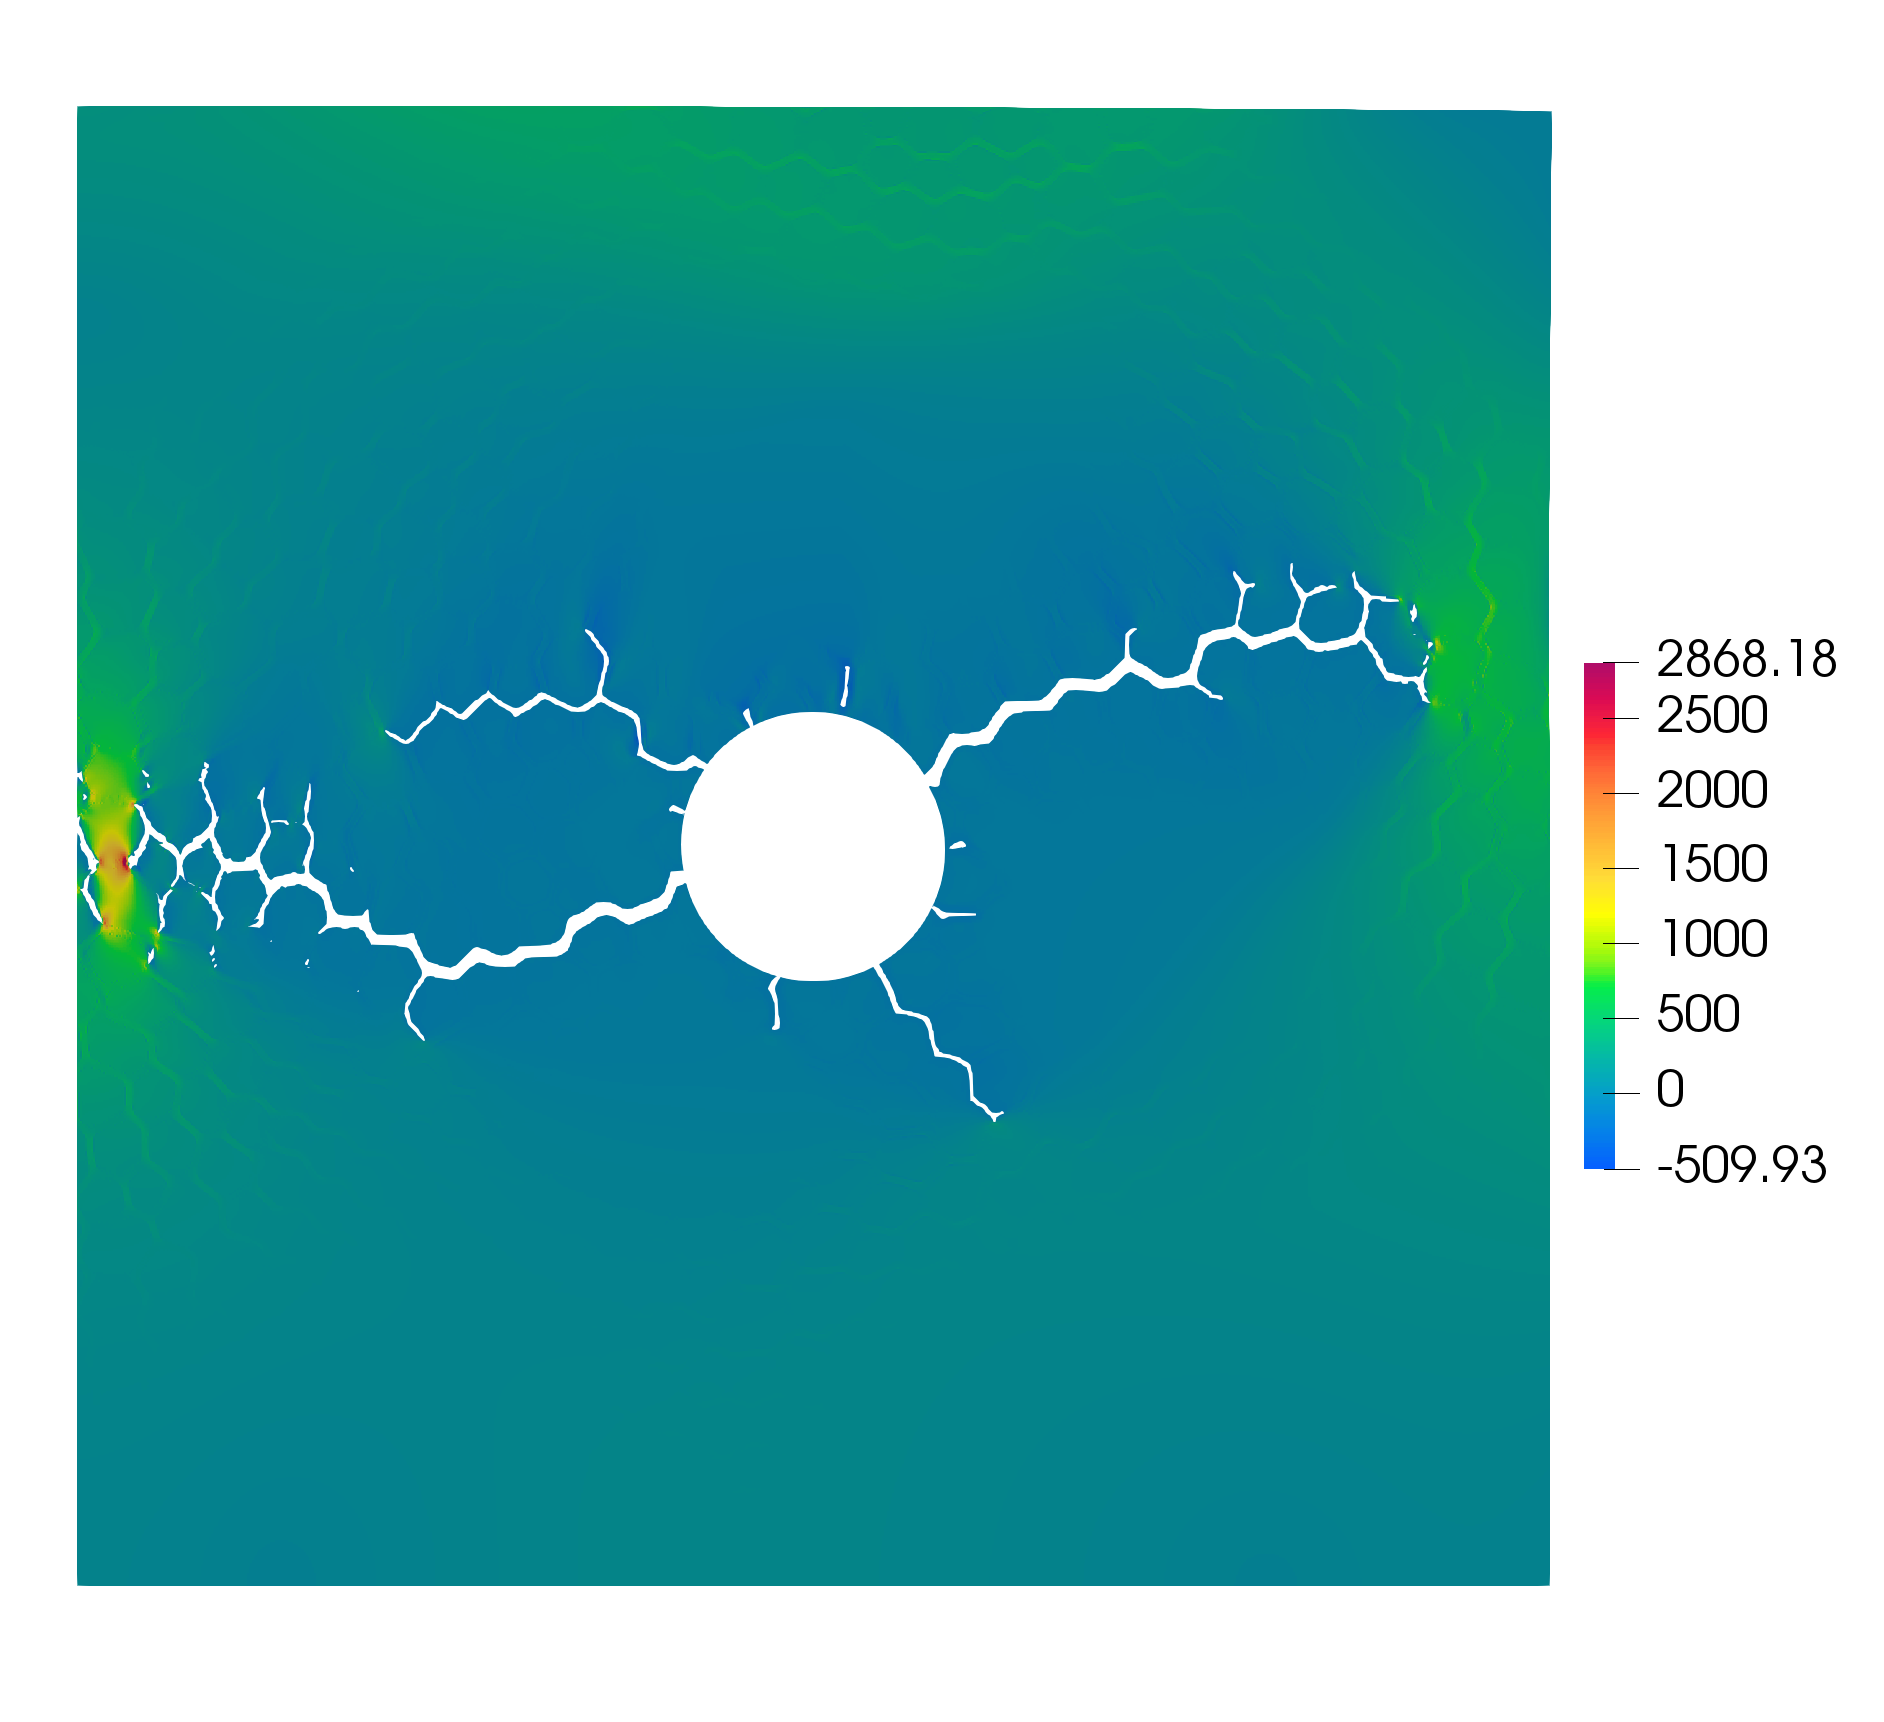
\includegraphics[width=\linewidth]{Chapter3/figures/r25_ext0_stress}
    \caption{}
  \end{subfigure}\\
  \begin{subfigure}[t]{0.32\linewidth}
    \centering
    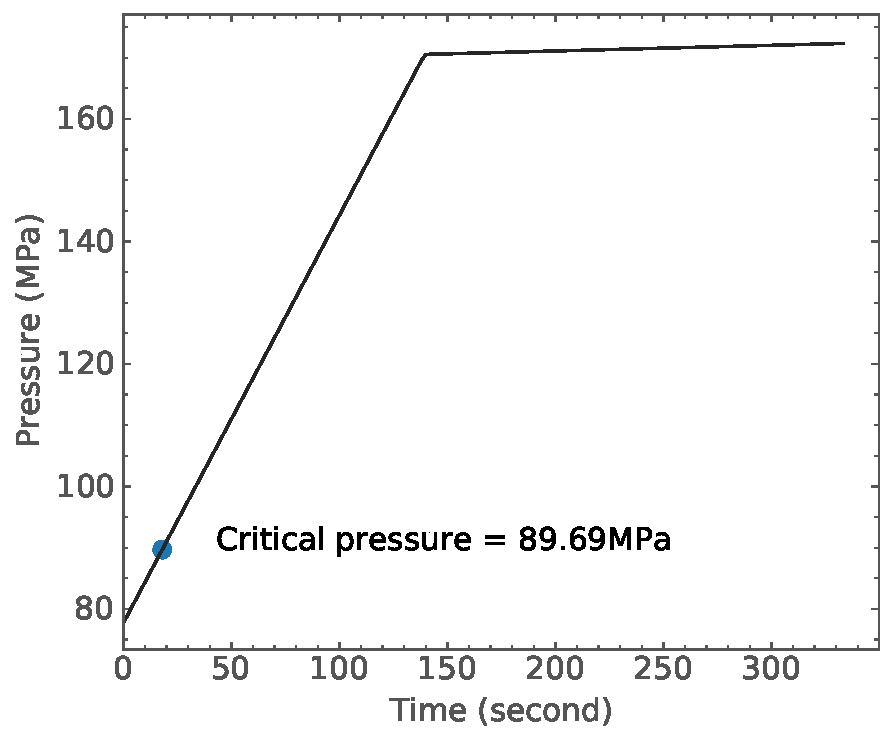
\includegraphics[width=\linewidth]{Chapter3/figures/bubble_pressure_r0.5_ext0_rod196}
    \caption{}
  \end{subfigure}
  \begin{subfigure}[t]{0.32\linewidth}
    \centering
    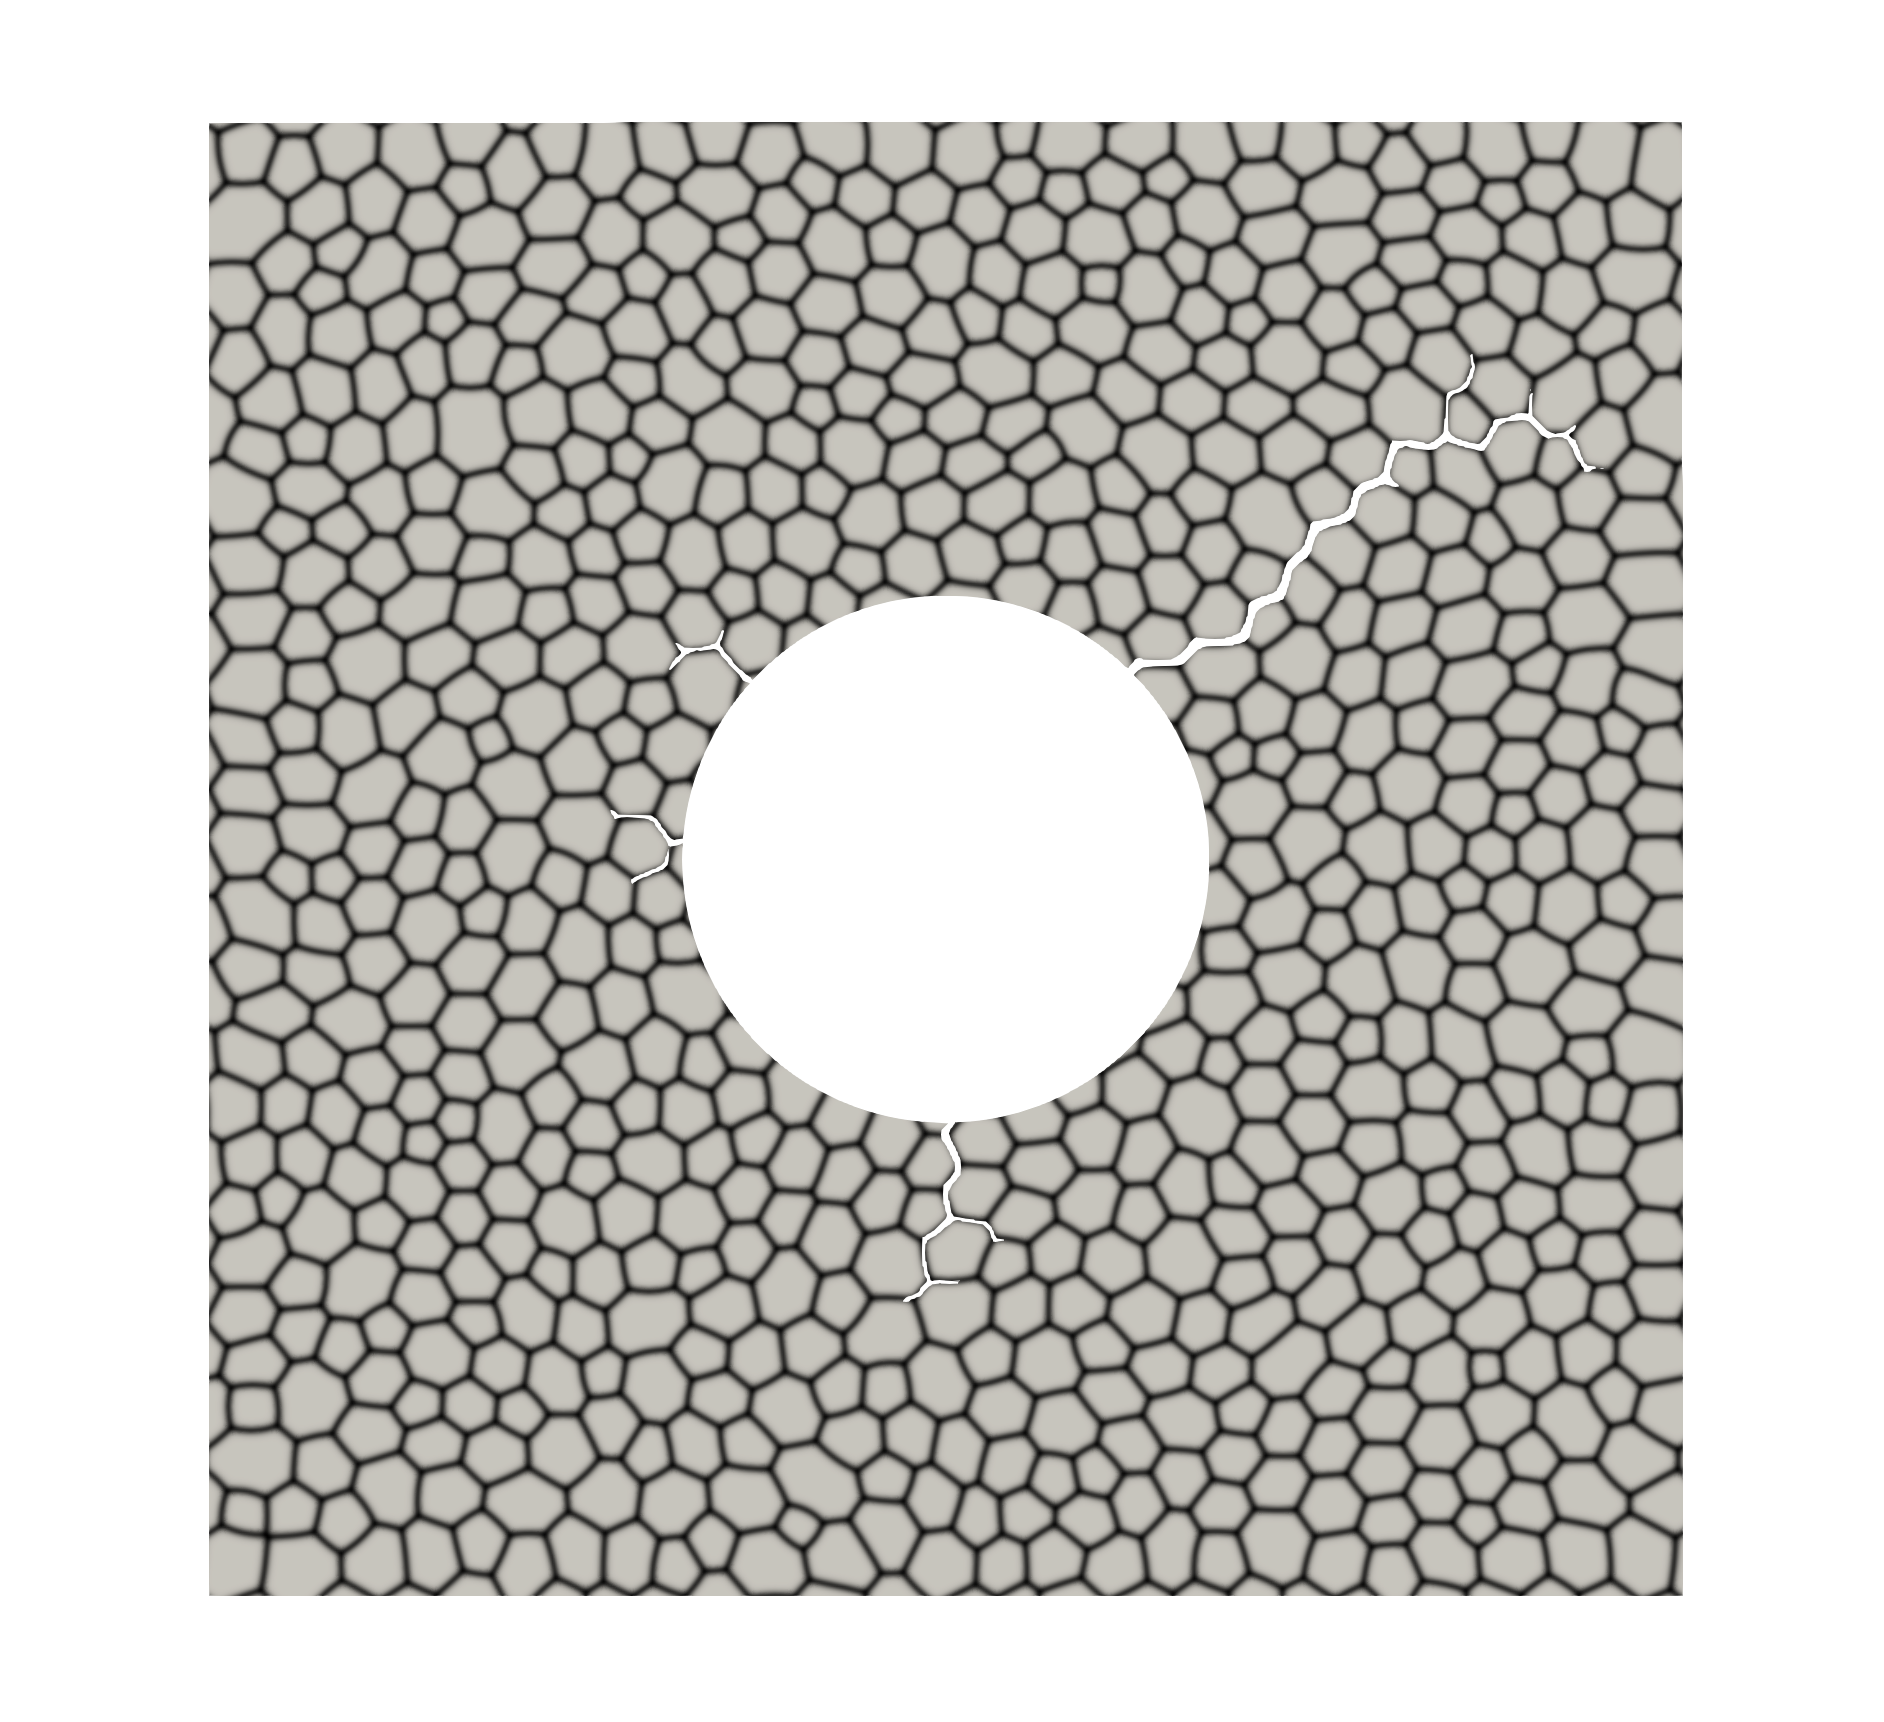
\includegraphics[width=\linewidth]{Chapter3/figures/r5_ext0}
    \caption{}
  \end{subfigure}
  \begin{subfigure}[t]{0.32\linewidth}
    \centering
    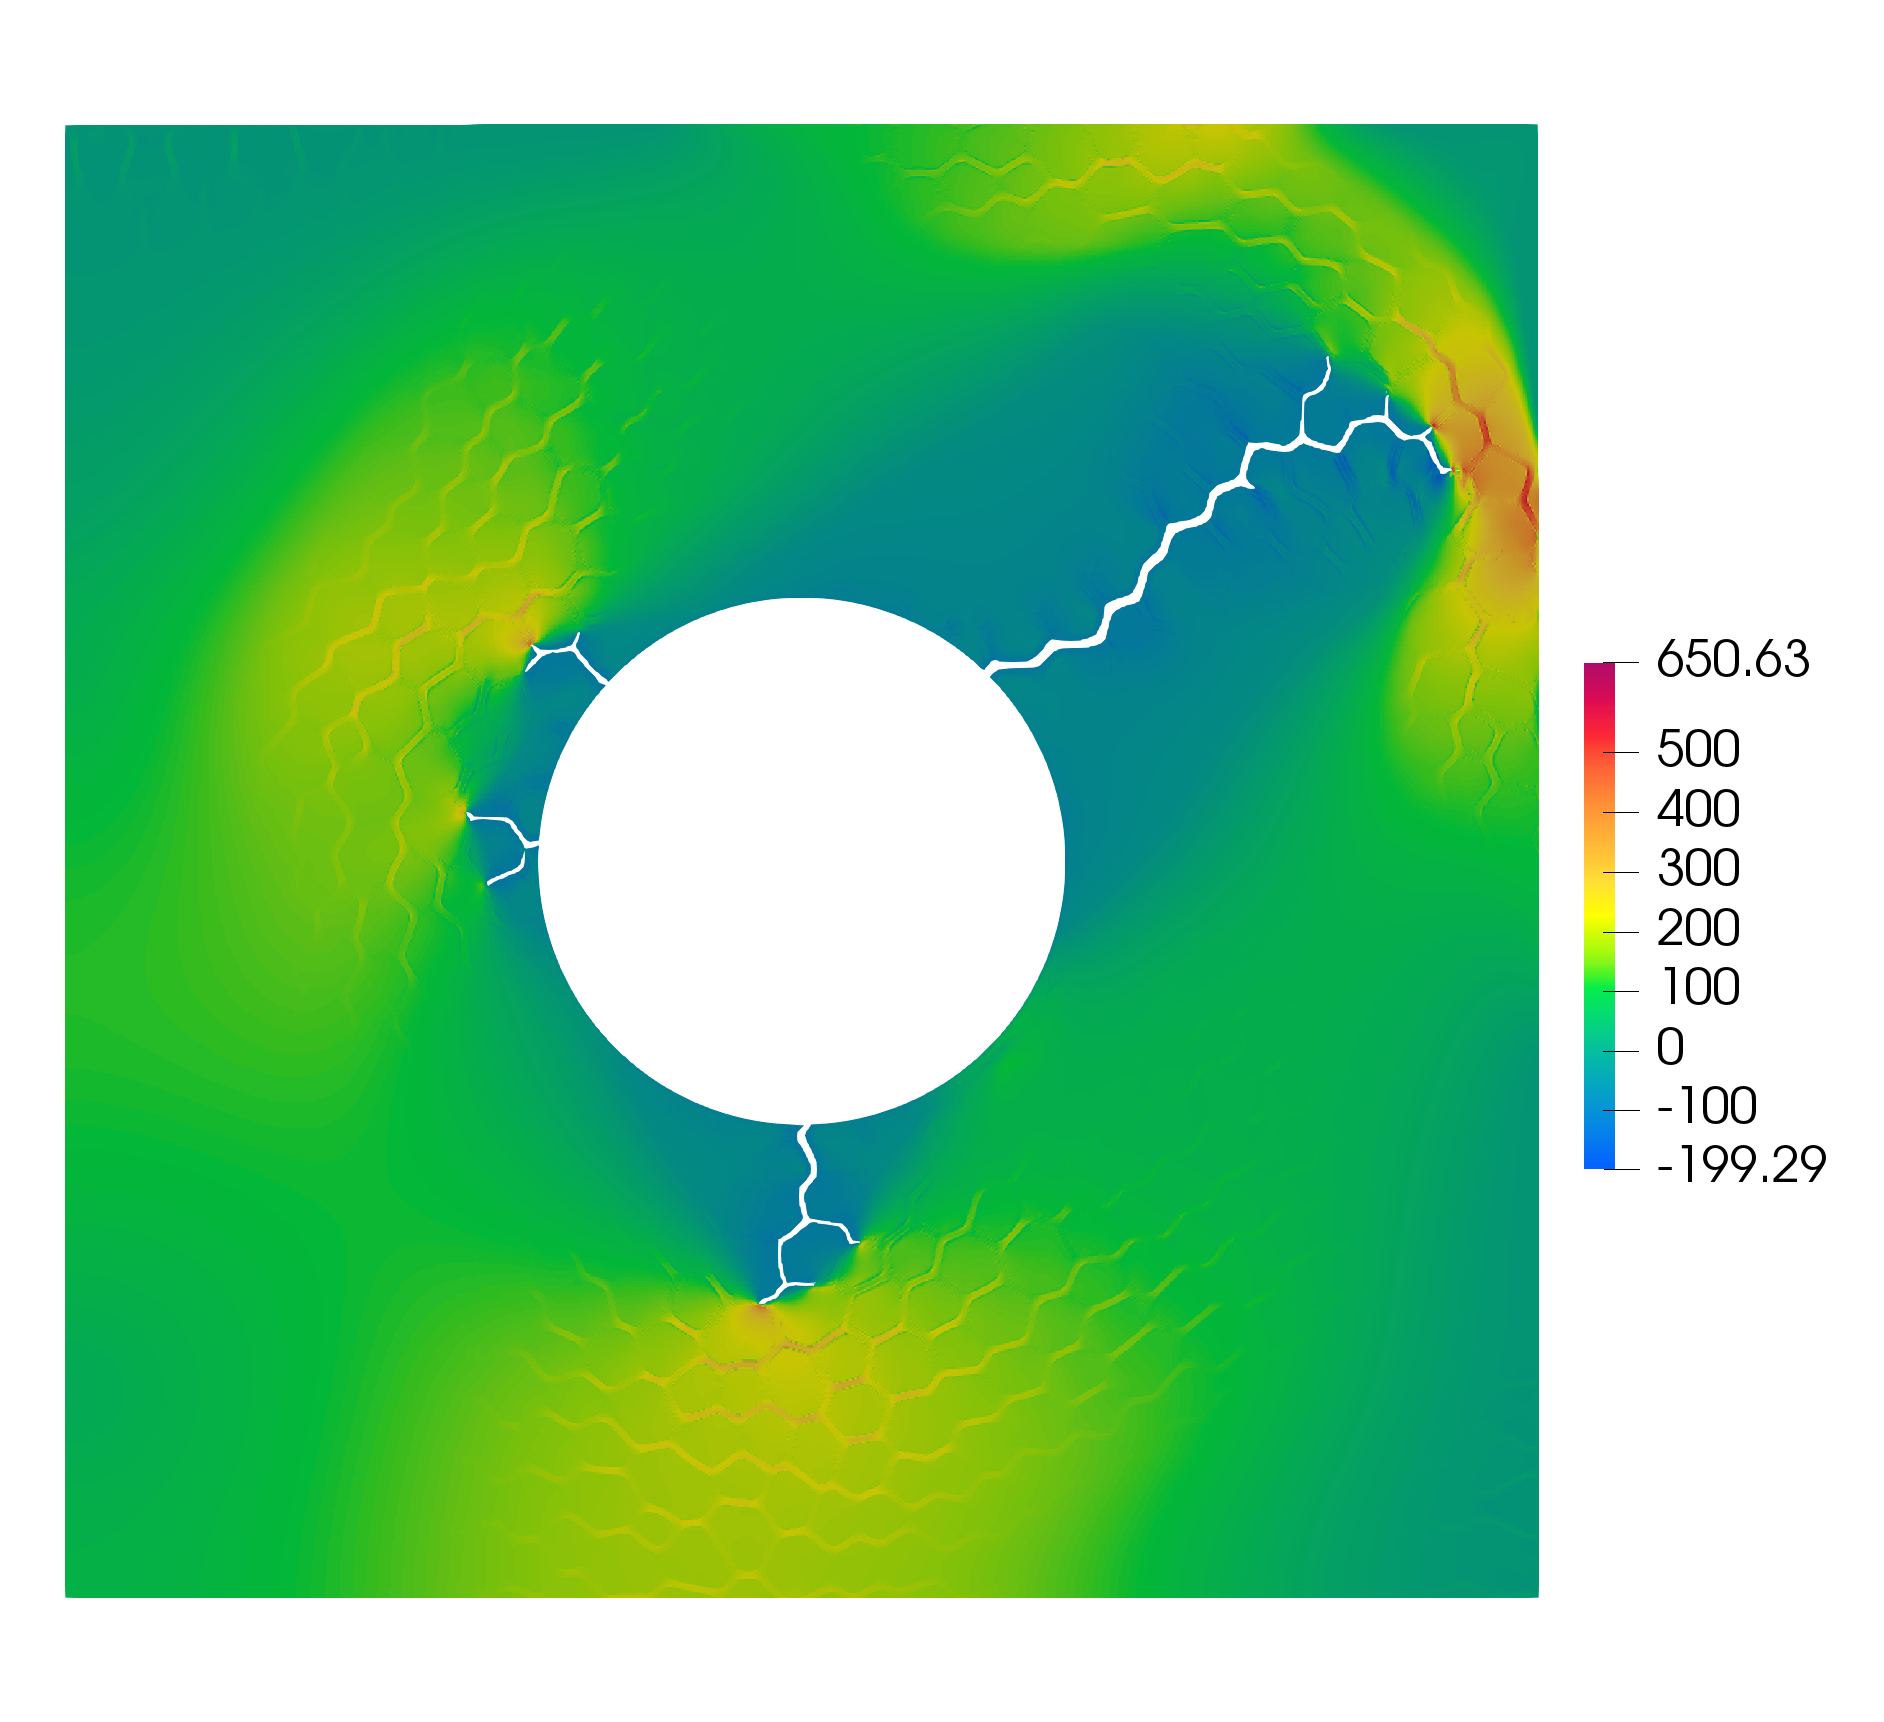
\includegraphics[width=\linewidth]{Chapter3/figures/r5_ext0_stress}
    \caption{}
  \end{subfigure}
  \caption[Crack propagation from bubbles with different sizes.]{Results for (a-c) the small bubble with radius \SI{0.25}{\micro\meter} and (d-f) the large bubble with radius \SI{0.25}{\micro\meter} (a, d) Pressure history. (b, e) Crack paths superimposed on the voronoi structure. (c, f) Contour plot of the maximum principal stress.}
  \label{fig:r25}
\end{figure}

In a fuel pellet system, external pressure can arise from fuel-cladding mechanical interaction. To study the effect of external pressure, different external pressures are applied on the top and right boundaries.  The results obtained from using three different external pressures, 0, \SI{30}{\mega\pascal}, and \SI{60}{\mega\pascal}, are shown in \Cref{fig:compare_external_pressure}. The critical pressure is significantly higher for larger external pressure values, while there is no qualitative change in the crack pattern.

\begin{figure}[htb!]
  \centering
  \begin{subfigure}[t]{0.32\linewidth}
    \centering
    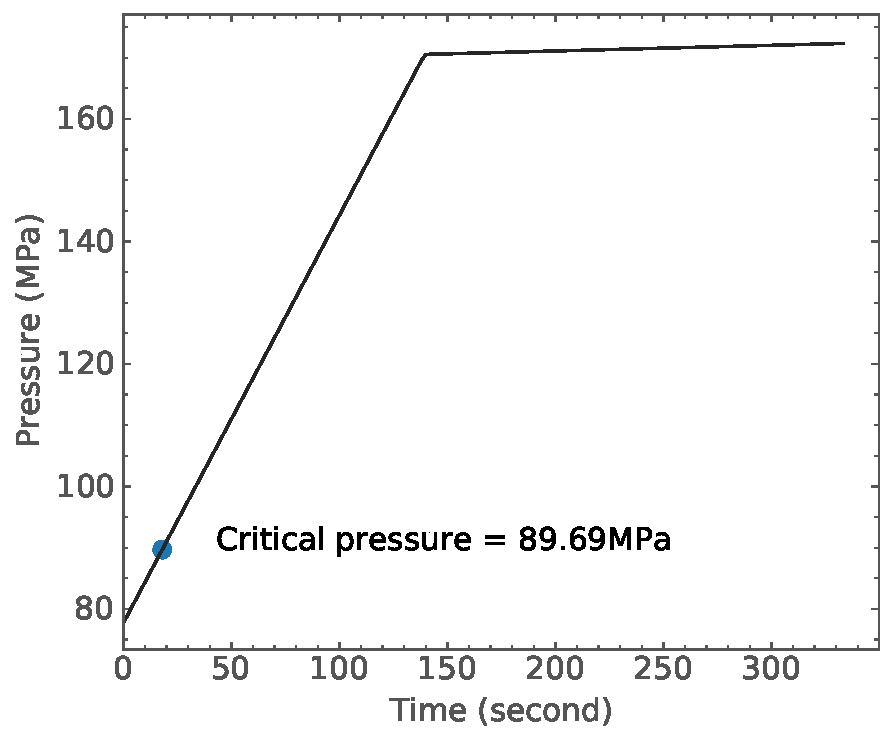
\includegraphics[width=\linewidth]{Chapter3/figures/bubble_pressure_r0.5_ext0_rod196}
    \caption{}
  \end{subfigure}
  \begin{subfigure}[t]{0.32\linewidth}
    \centering
    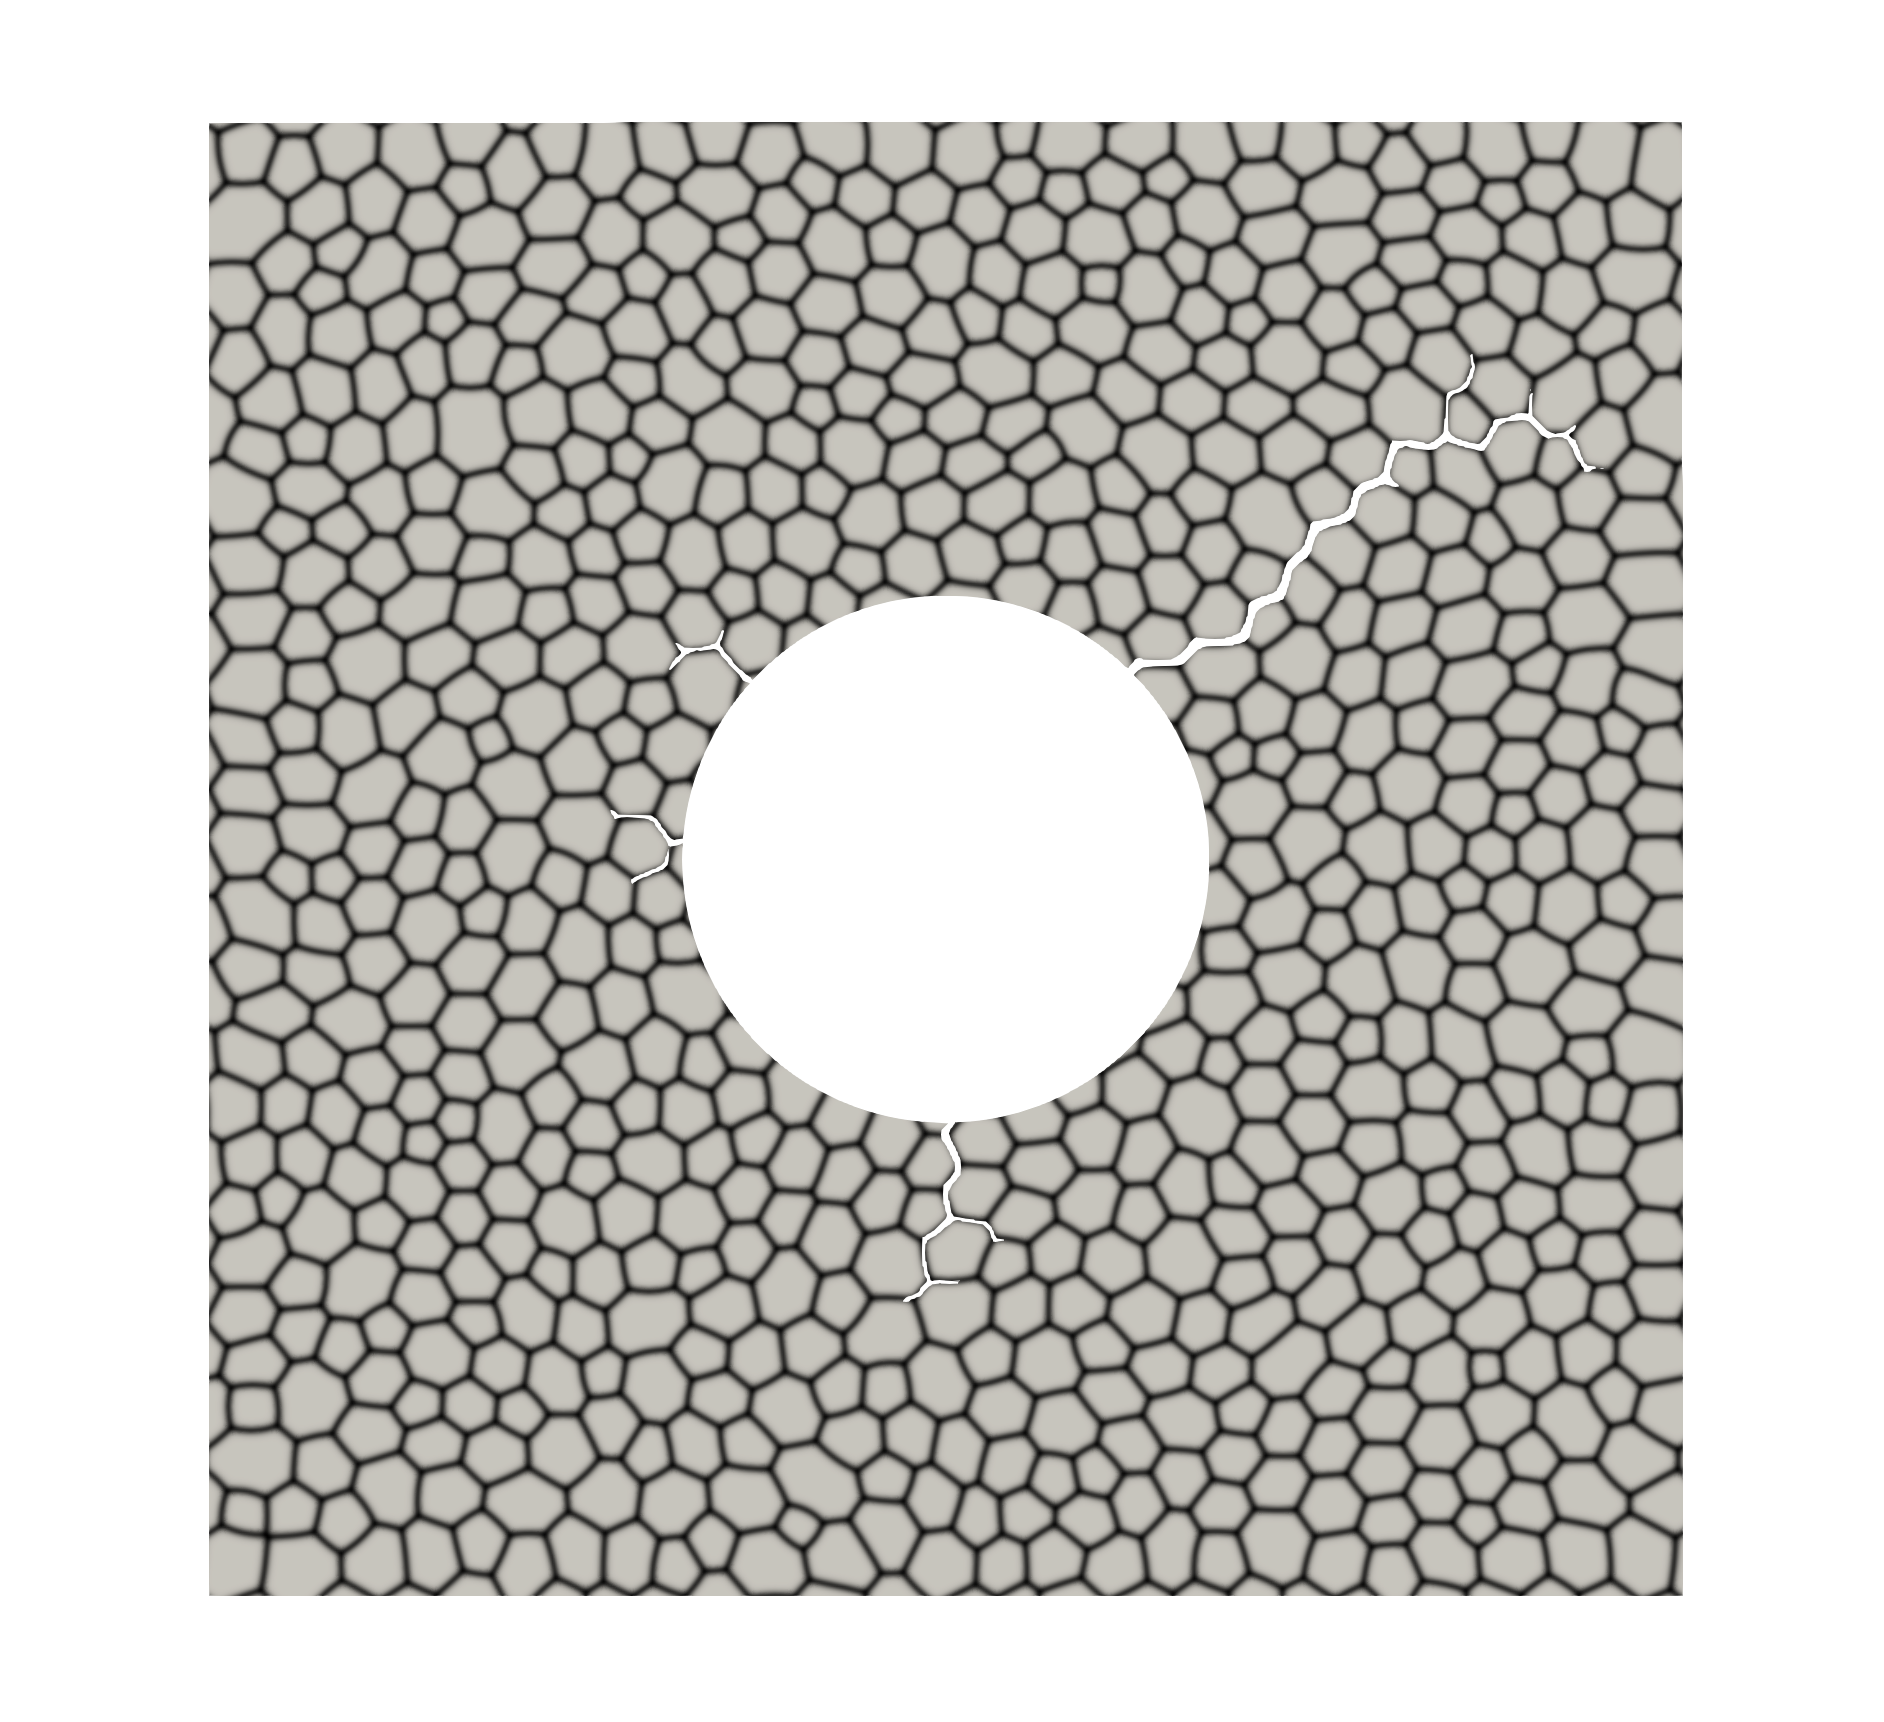
\includegraphics[width=\linewidth]{Chapter3/figures/r5_ext0}
    \caption{}
  \end{subfigure}
  \begin{subfigure}[t]{0.32\linewidth}
    \centering
    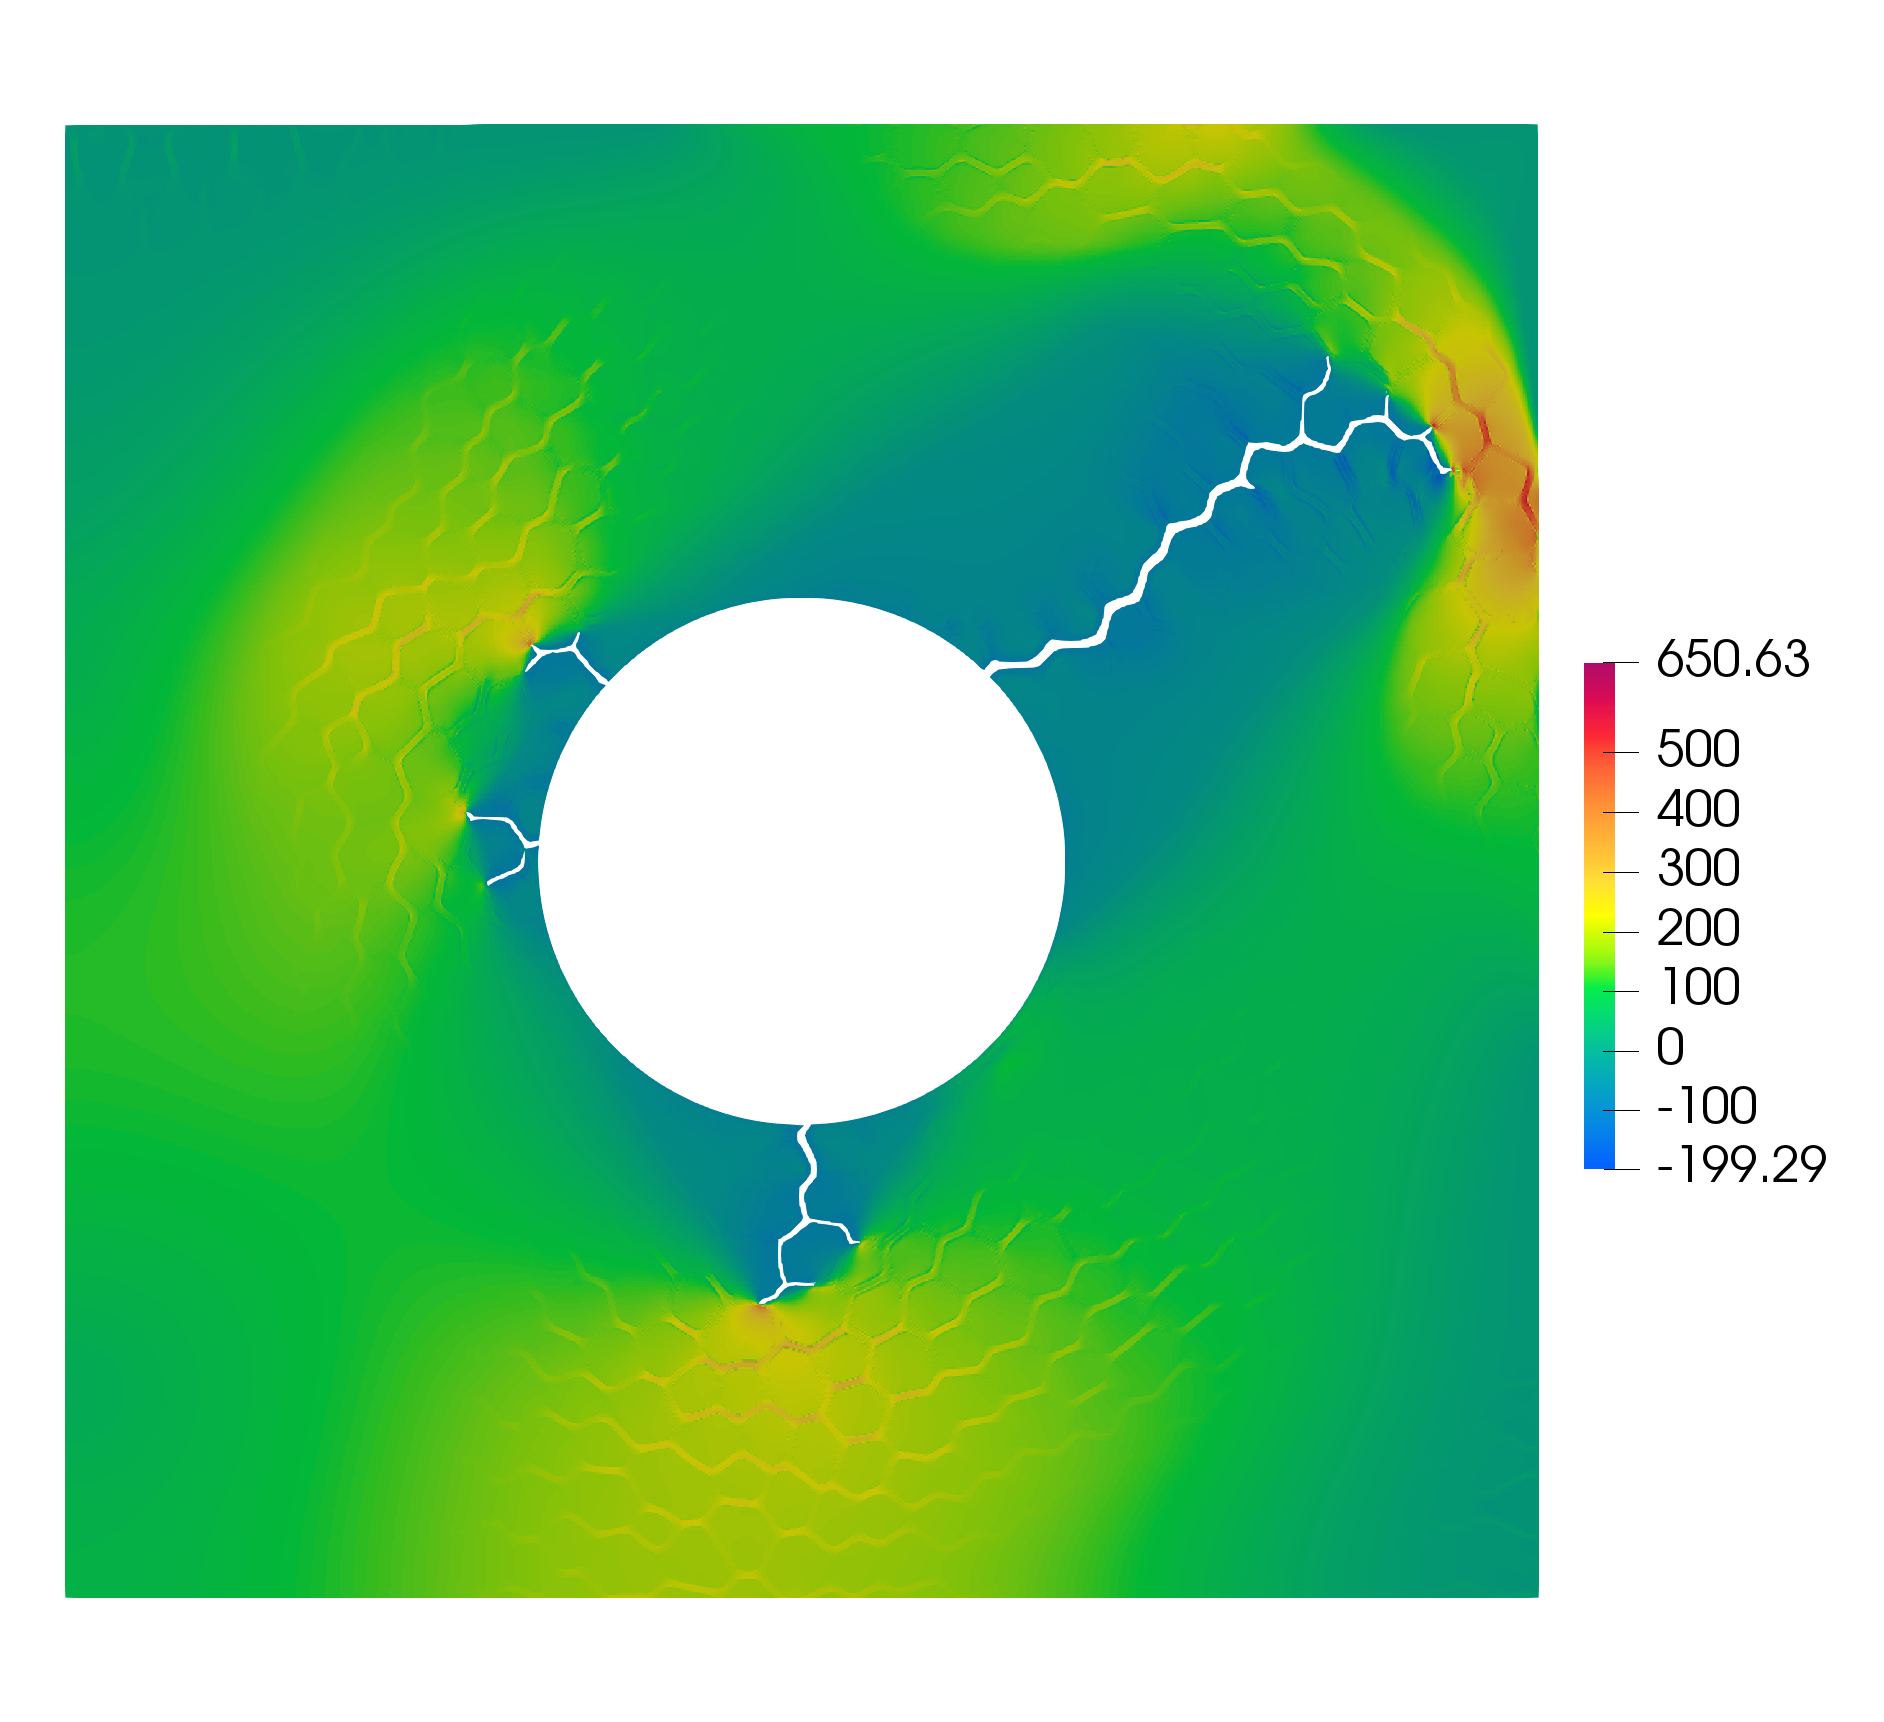
\includegraphics[width=\linewidth]{Chapter3/figures/r5_ext0_stress}
    \caption{}
  \end{subfigure}\\
  \begin{subfigure}[t]{0.32\linewidth}
    \centering
    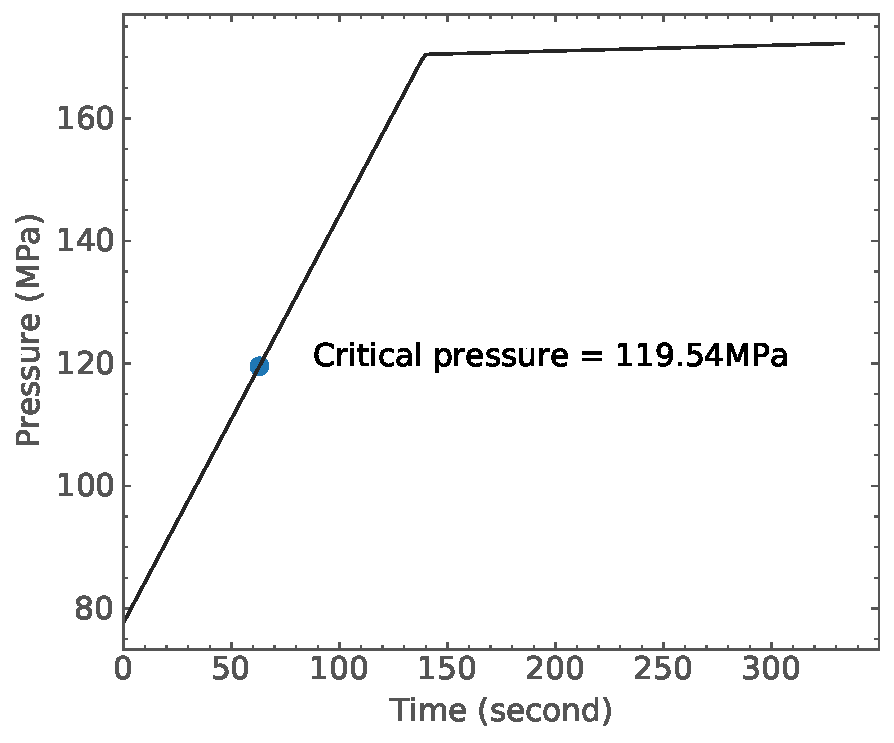
\includegraphics[width=\linewidth]{Chapter3/figures/bubble_pressure_r0.5_ext30_rod196}
    \caption{}
  \end{subfigure}
  \begin{subfigure}[t]{0.32\linewidth}
    \centering
    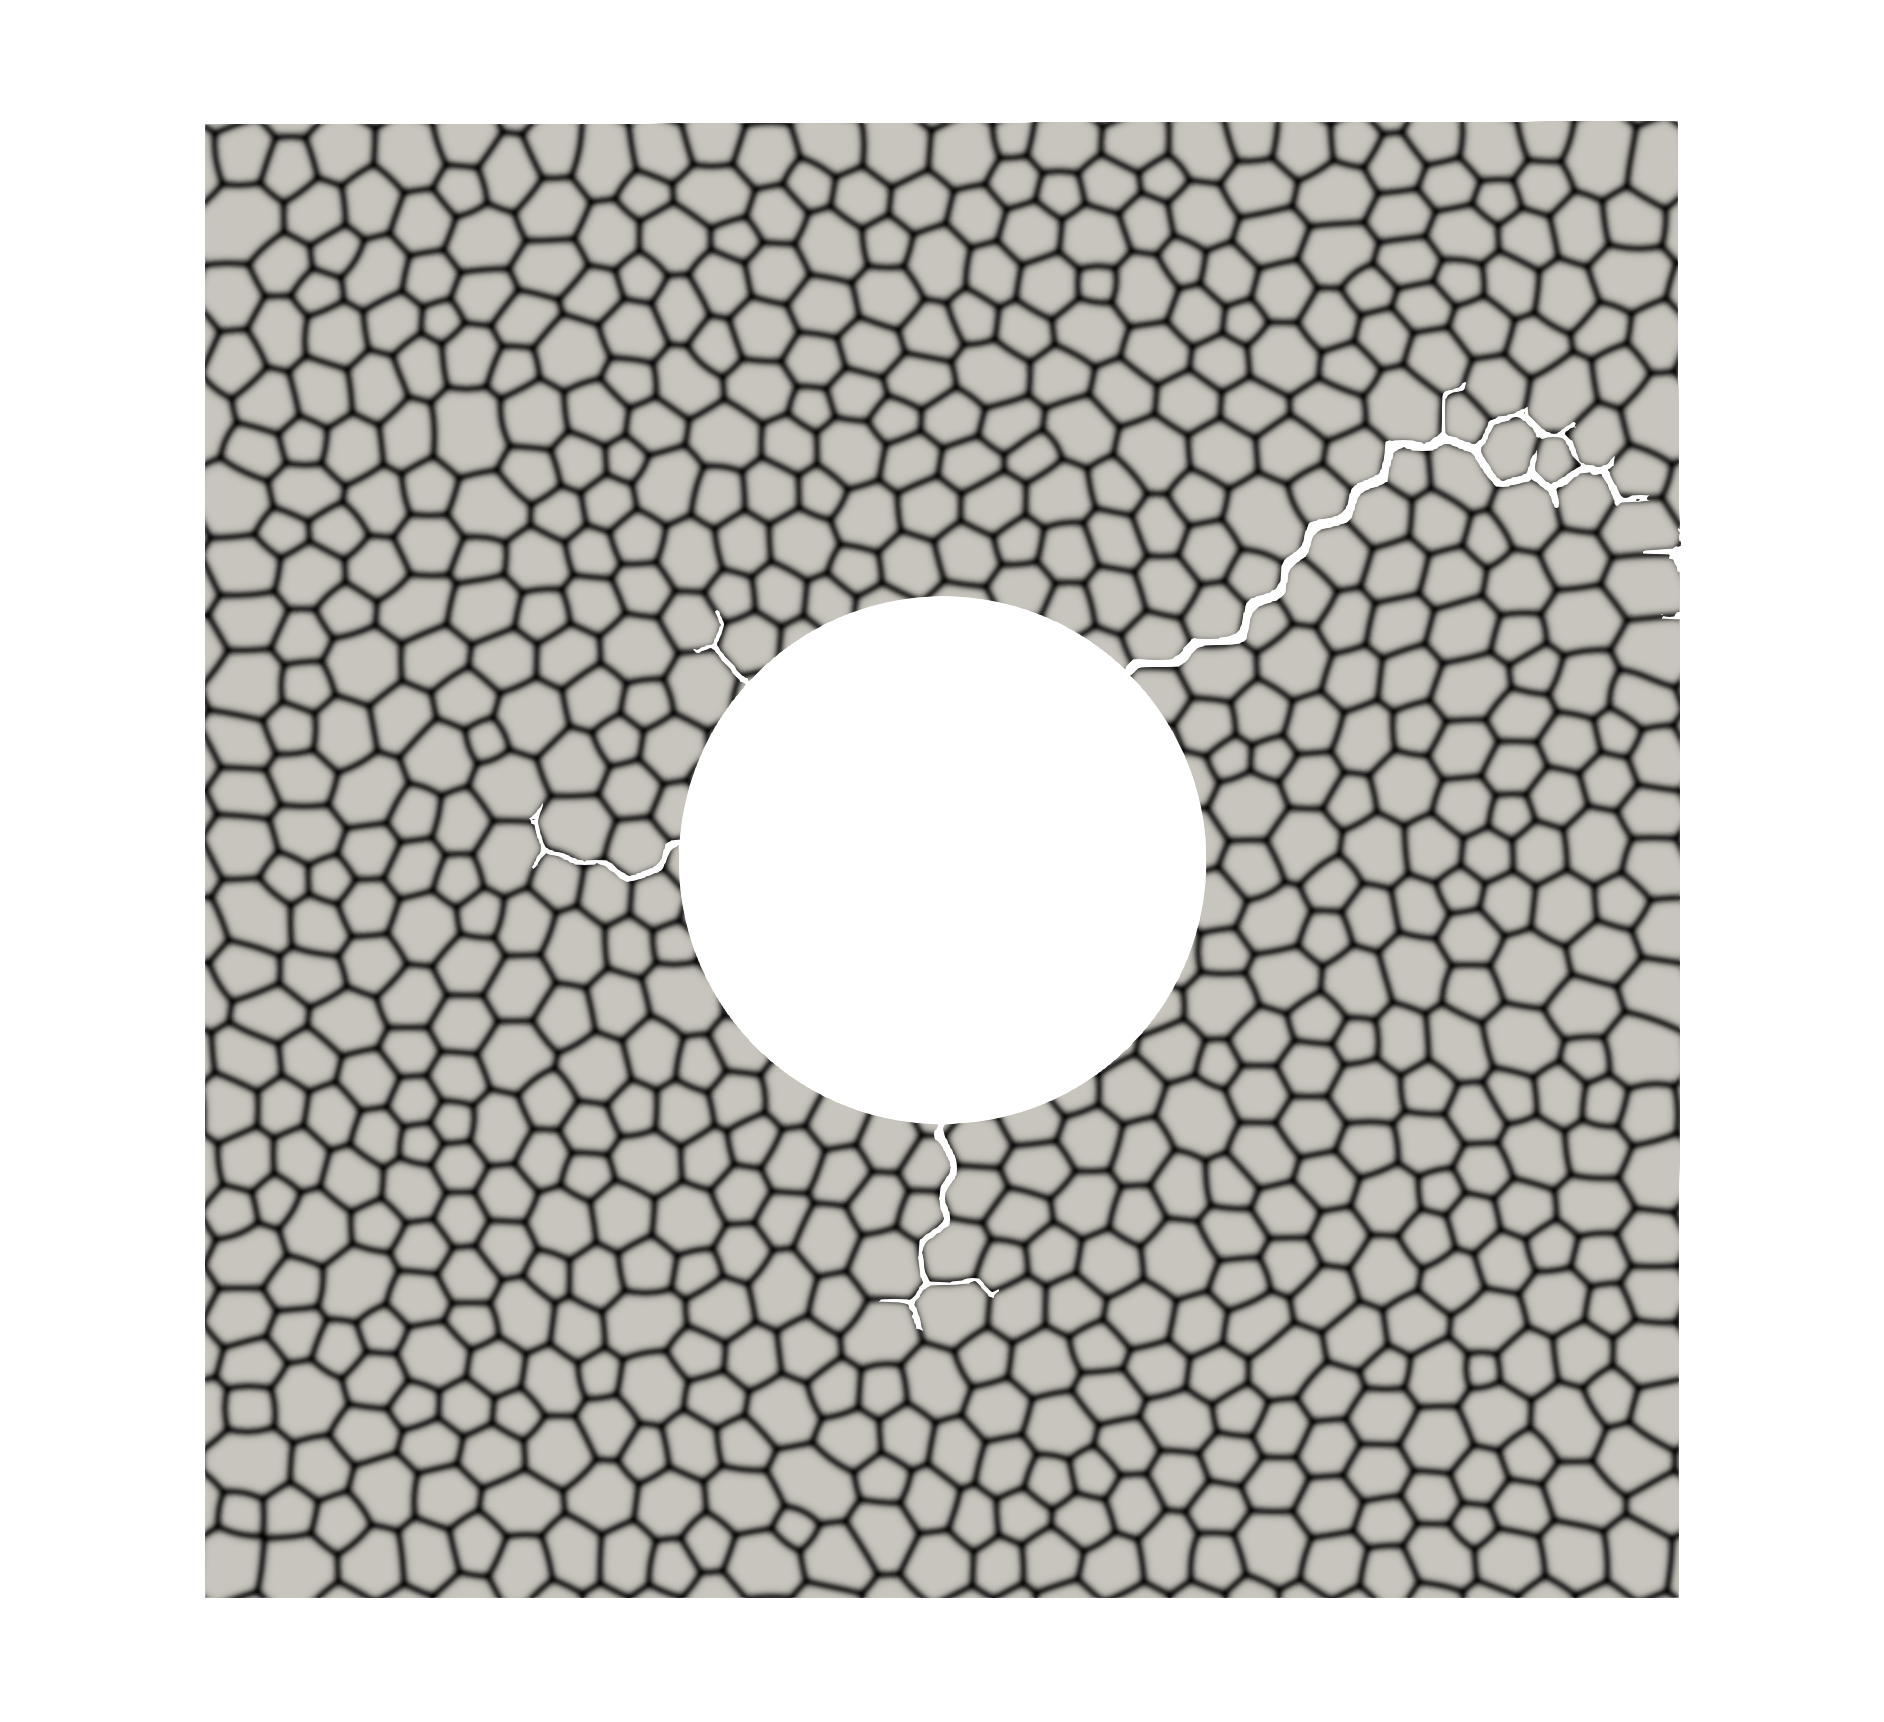
\includegraphics[width=\linewidth]{Chapter3/figures/r5_ext30}
    \caption{}
  \end{subfigure}
  \begin{subfigure}[t]{0.32\linewidth}
    \centering
    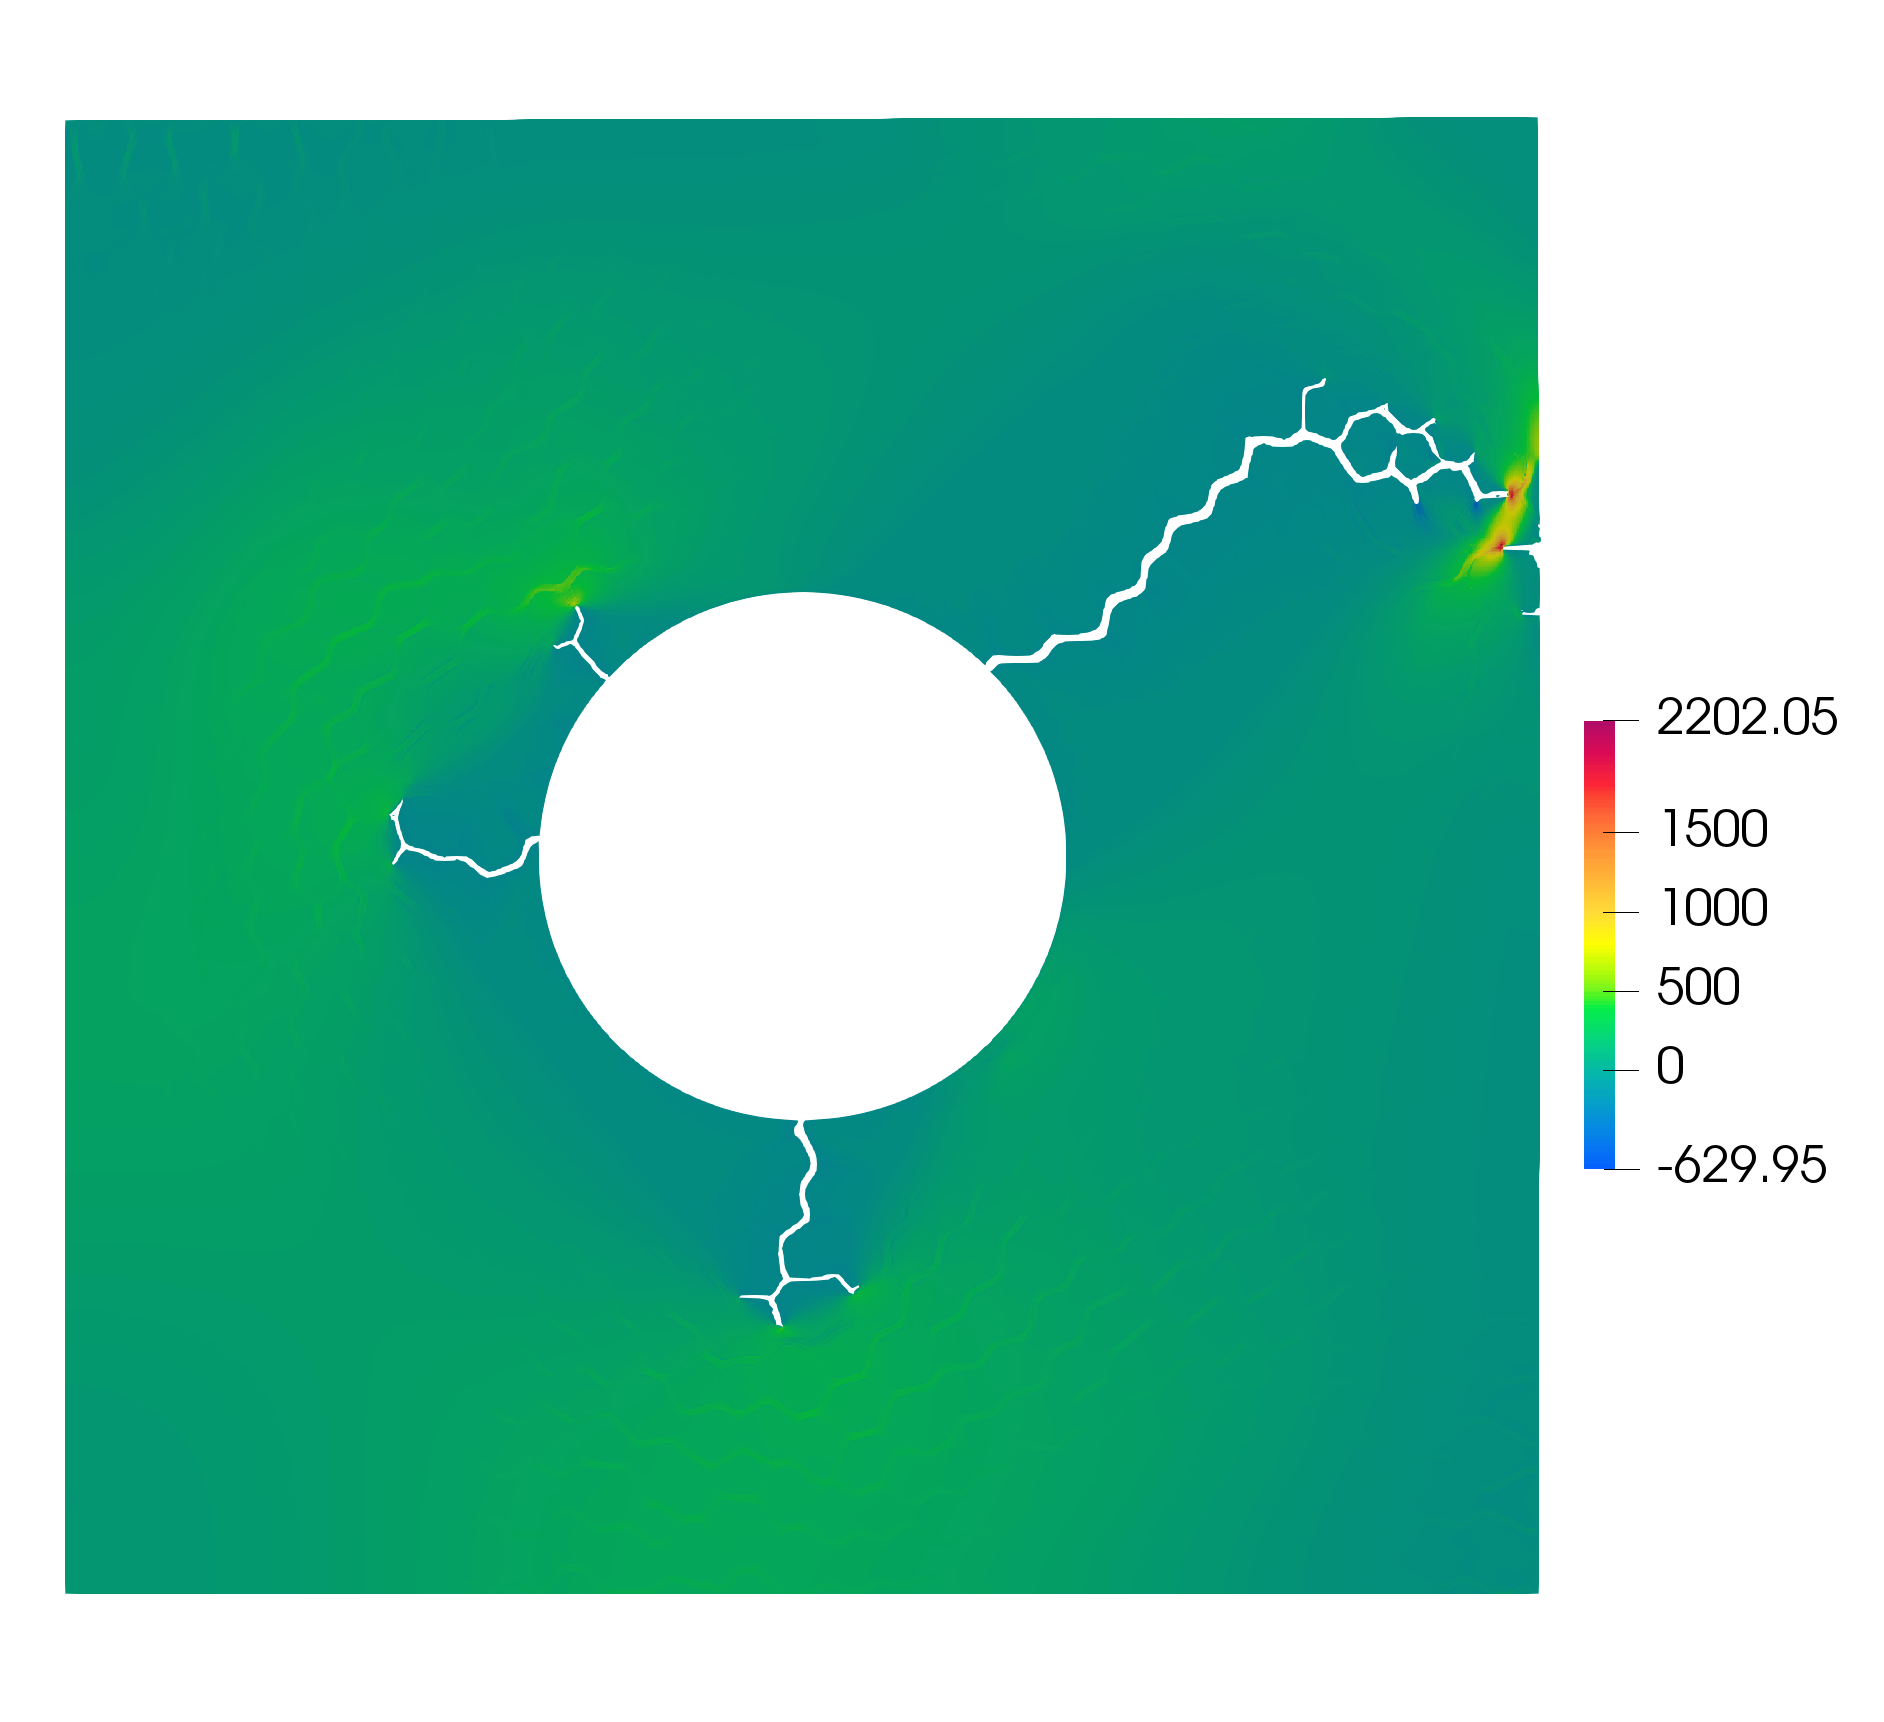
\includegraphics[width=\linewidth]{Chapter3/figures/r5_ext30_stress}
    \caption{}
  \end{subfigure}\\
  \begin{subfigure}[t]{0.32\linewidth}
    \centering
    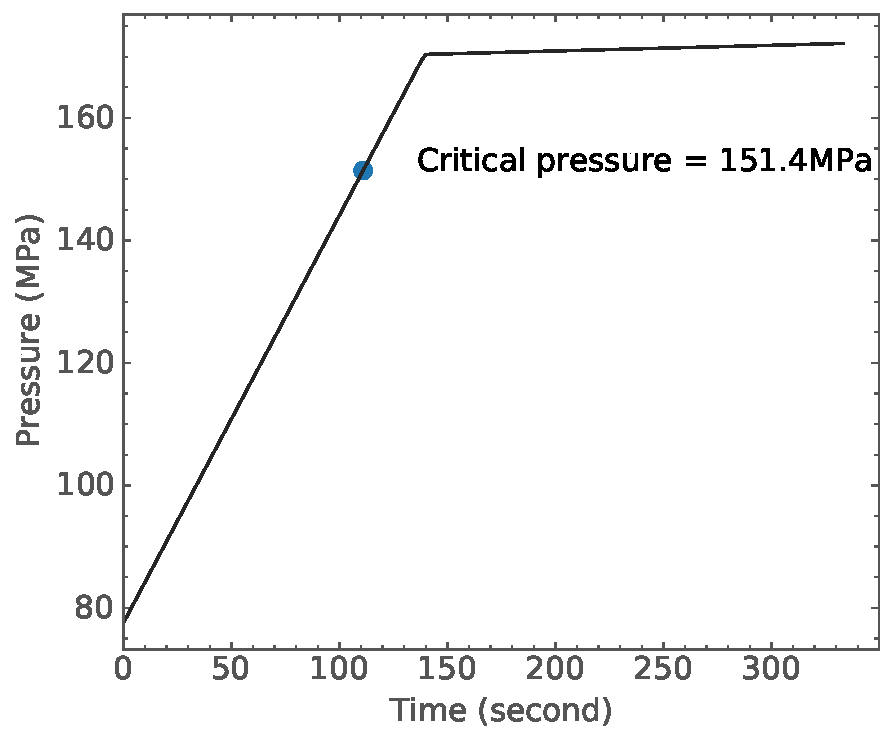
\includegraphics[width=\linewidth]{Chapter3/figures/bubble_pressure_r0.5_ext60_rod196}
    \caption{}
  \end{subfigure}
  \begin{subfigure}[t]{0.32\linewidth}
    \centering
    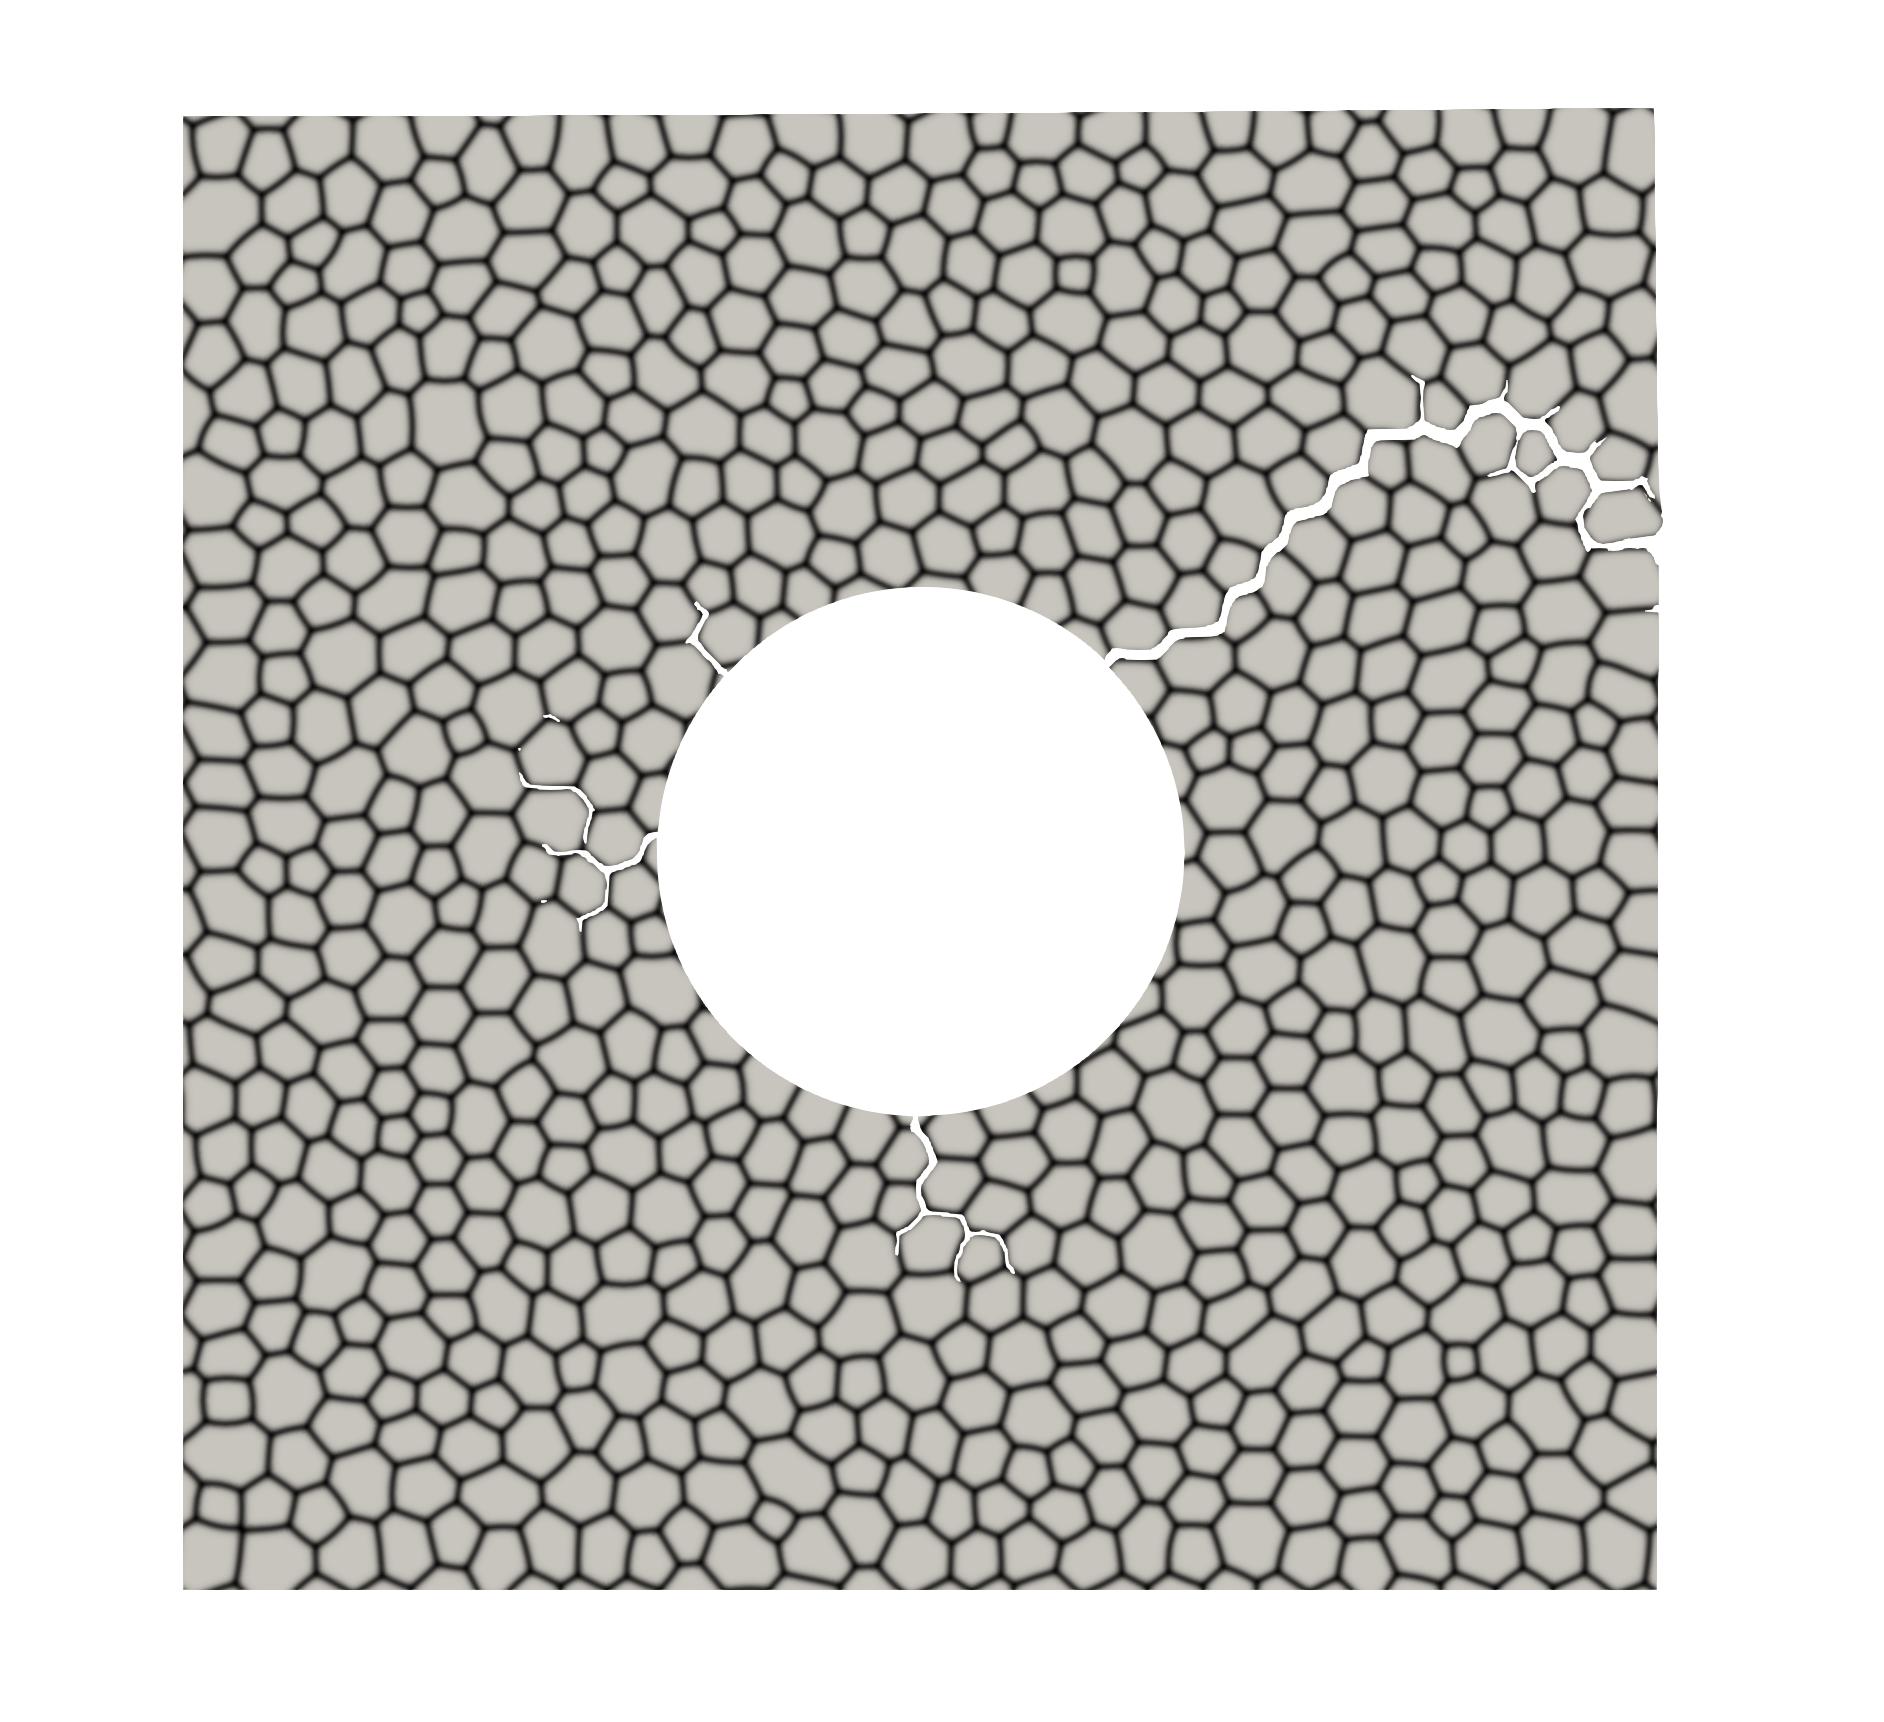
\includegraphics[width=\linewidth]{Chapter3/figures/r5_ext60}
    \caption{}
  \end{subfigure}
  \begin{subfigure}[t]{0.32\linewidth}
    \centering
    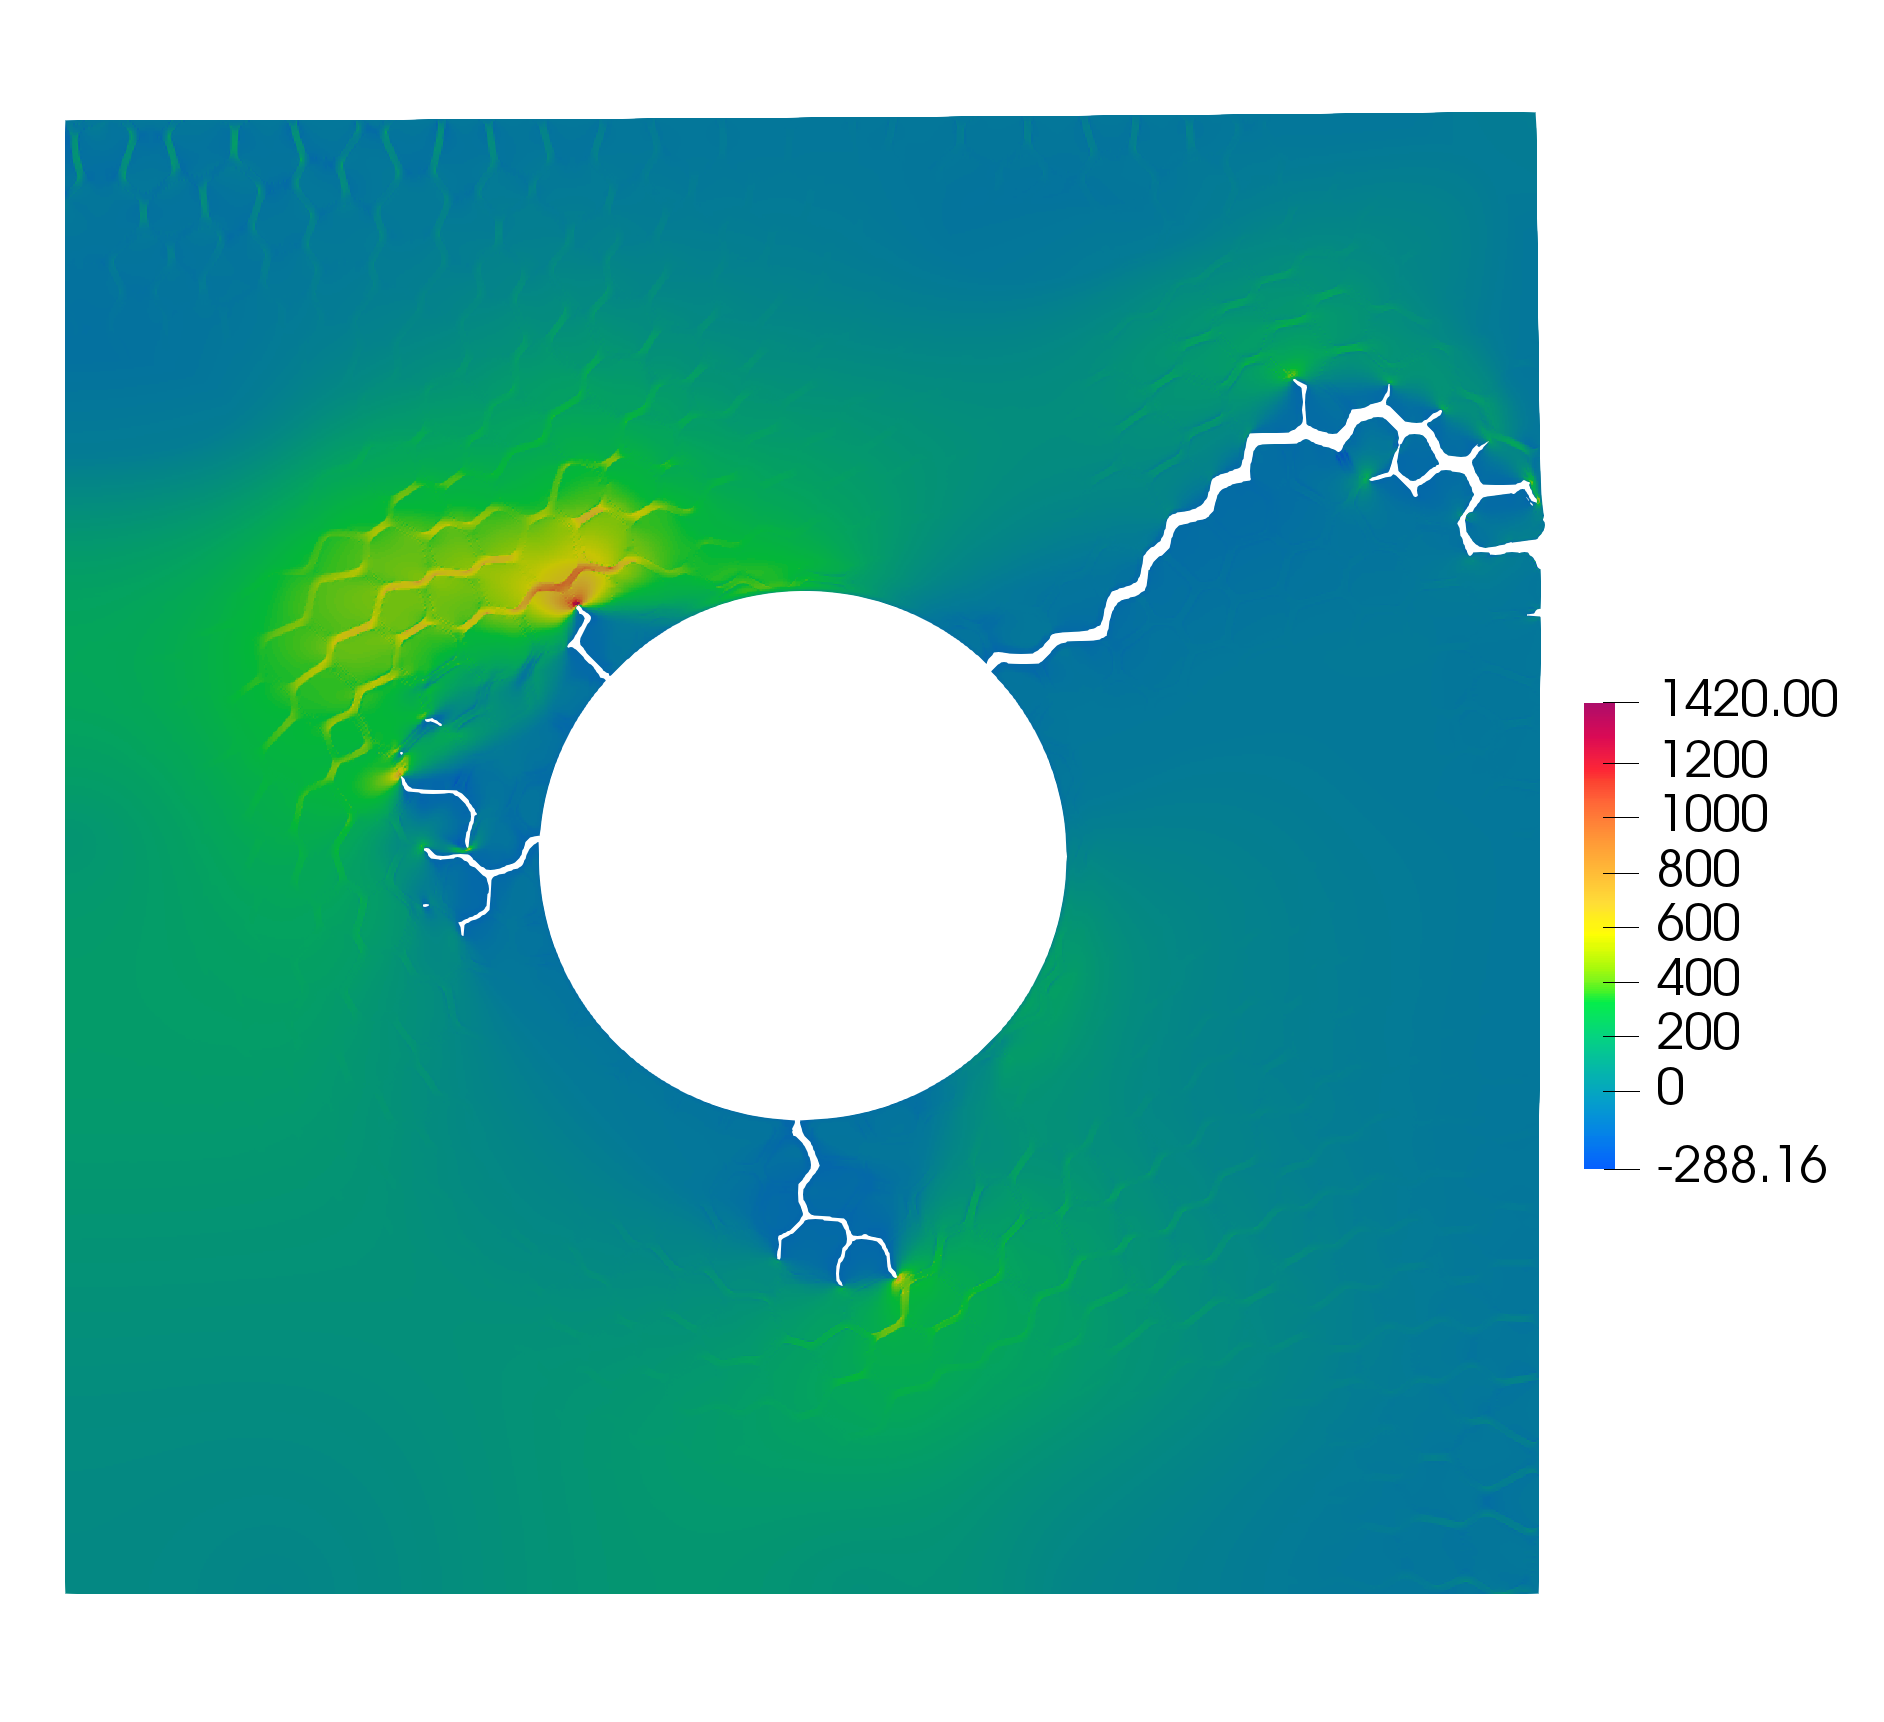
\includegraphics[width=\linewidth]{Chapter3/figures/r5_ext60_stress}
    \caption{}
  \end{subfigure}
  \caption[Crack propagation with different external pressure loadings.]{ Results for bubble radius \SI{0.5}{\micro\meter} and external pressure (a-c) \SI{0}{\mega\pascal}, (d-f) \SI{30}{\mega\pascal}, (g-i) \SI{60}{\mega\pascal}. (a, d, g) Pressure history. (b, e, h) Crack paths superimposed on the voronoi structure. (c, f, i) Contour plot of the maximum principal stress. }
  \label{fig:compare_external_pressure}
\end{figure}

%%%%%%%%%%%%%%%%%%%%%%%%%%%%%%%%%%%%%%%%%%%%%%%%%%%%%%%%%%%%%%%%%%%%%%%%%%%%%%%%%%%%%%%%%%%
%%%%%%%%%%%%%%%%%%%%%%%%%%%%%%%%%%%%%%%%%%%%%%%%%%%%%%%%%%%%%%%%%%%%%%%%%%%%%%%%%%%%%%%%%%%
%%%%%%%%%%%%%%%%%%%%%%%%%%%%%%%%%%%%%%%%%%%%%%%%%%%%%%%%%%%%%%%%%%%%%%%%%%%%%%%%%%%%%%%%%%%
%%%%%%%%%%%%%%%%%%%%%%%%%%%%%%%%%%%%%%%%%%%%%%%%%%%%%%%%%%%%%%%%%%%%%%%%%%%%%%%%%%%%%%%%%%%
%%%%%%%%%%%%%%%%%%%%%%%%%%%%%%%%%%%%%%%%%%%%%%%%%%%%%%%%%%%%%%%%%%%%%%%%%%%%%%%%%%%%%%%%%%%
%%%%%%%%%%%%%%%%%%%%%%%%%%%%%%%%%%%%%%%%%%%%%%%%%%%%%%%%%%%%%%%%%%%%%%%%%%%%%%%%%%%%%%%%%%%
%%%%%%%%%%%%%%%%%%%%%%%%%%%%%%%%%%%%%%%%%%%%%%%%%%%%%%%%%%%%%%%%%%%%%%%%%%%%%%%%%%%%%%%%%%%
%%%%%%%%%%%%%%%%%%%%%%%%%%%%%%%%%%%%%%%%%%%%%%%%%%%%%%%%%%%%%%%%%%%%%%%%%%%%%%%%%%%%%%%%%%%
%%%%%%%%%%%%%%%%%%%%%%%%%%%%%%%%%%%%%%%%%%%%%%%%%%%%%%%%%%%%%%%%%%%%%%%%%%%%%%%%%%%%%%%%%%%
%%%%%%%%%%%%%%%%%%%%%%%%%%%%%%%%%%%%%%%%%%%%%%%%%%%%%%%%%%%%%%%%%%%%%%%%%%%%%%%%%%%%%%%%%%%
\subsubsection{Multi-bubble interaction}

We next investigate the effect of the spatial distribution of the gas bubbles on fragment size. To that end, dimensions are expressed in dimensionless form in this section. With the origin of the coordinate system placed at the lower left corner of the REV, two cases are considered:
\begin{itemize}
  \item Two bubbles with centers at $\left( \dfrac{2}{15}L, \dfrac{7}{15}L \right)$ and $\left( \dfrac{7}{15}L, \dfrac{2}{15}L \right)$.
  \item Three bubbles with centers at $\left( \dfrac{1}{6}L, \dfrac{8}{15}L \right)$, $\left( \dfrac{8}{15}L, \dfrac{1}{6}L \right)$, and $\left( \dfrac{8}{15}L, \dfrac{8}{15}L \right)$.
\end{itemize}
All bubbles have a radius of $\dfrac{1}{12}L$. Results are shown in \Cref{fig:compare_bubble_distribution}. It is observed that the crack paths in cases involving multiple bubbles is strongly affected by the positions of the bubbles relative to each other: Cracks prefer to connect neighboring bubbles. Fully developed cracks and bubbles form a fragment at the lower-left corner in both cases. These fragments consist of multiple grains, and their sizes are affected by the spatial distribution of bubbles.

\begin{figure}[htb!]
  \centering
  \begin{subfigure}[t]{0.4\linewidth}
    \centering
    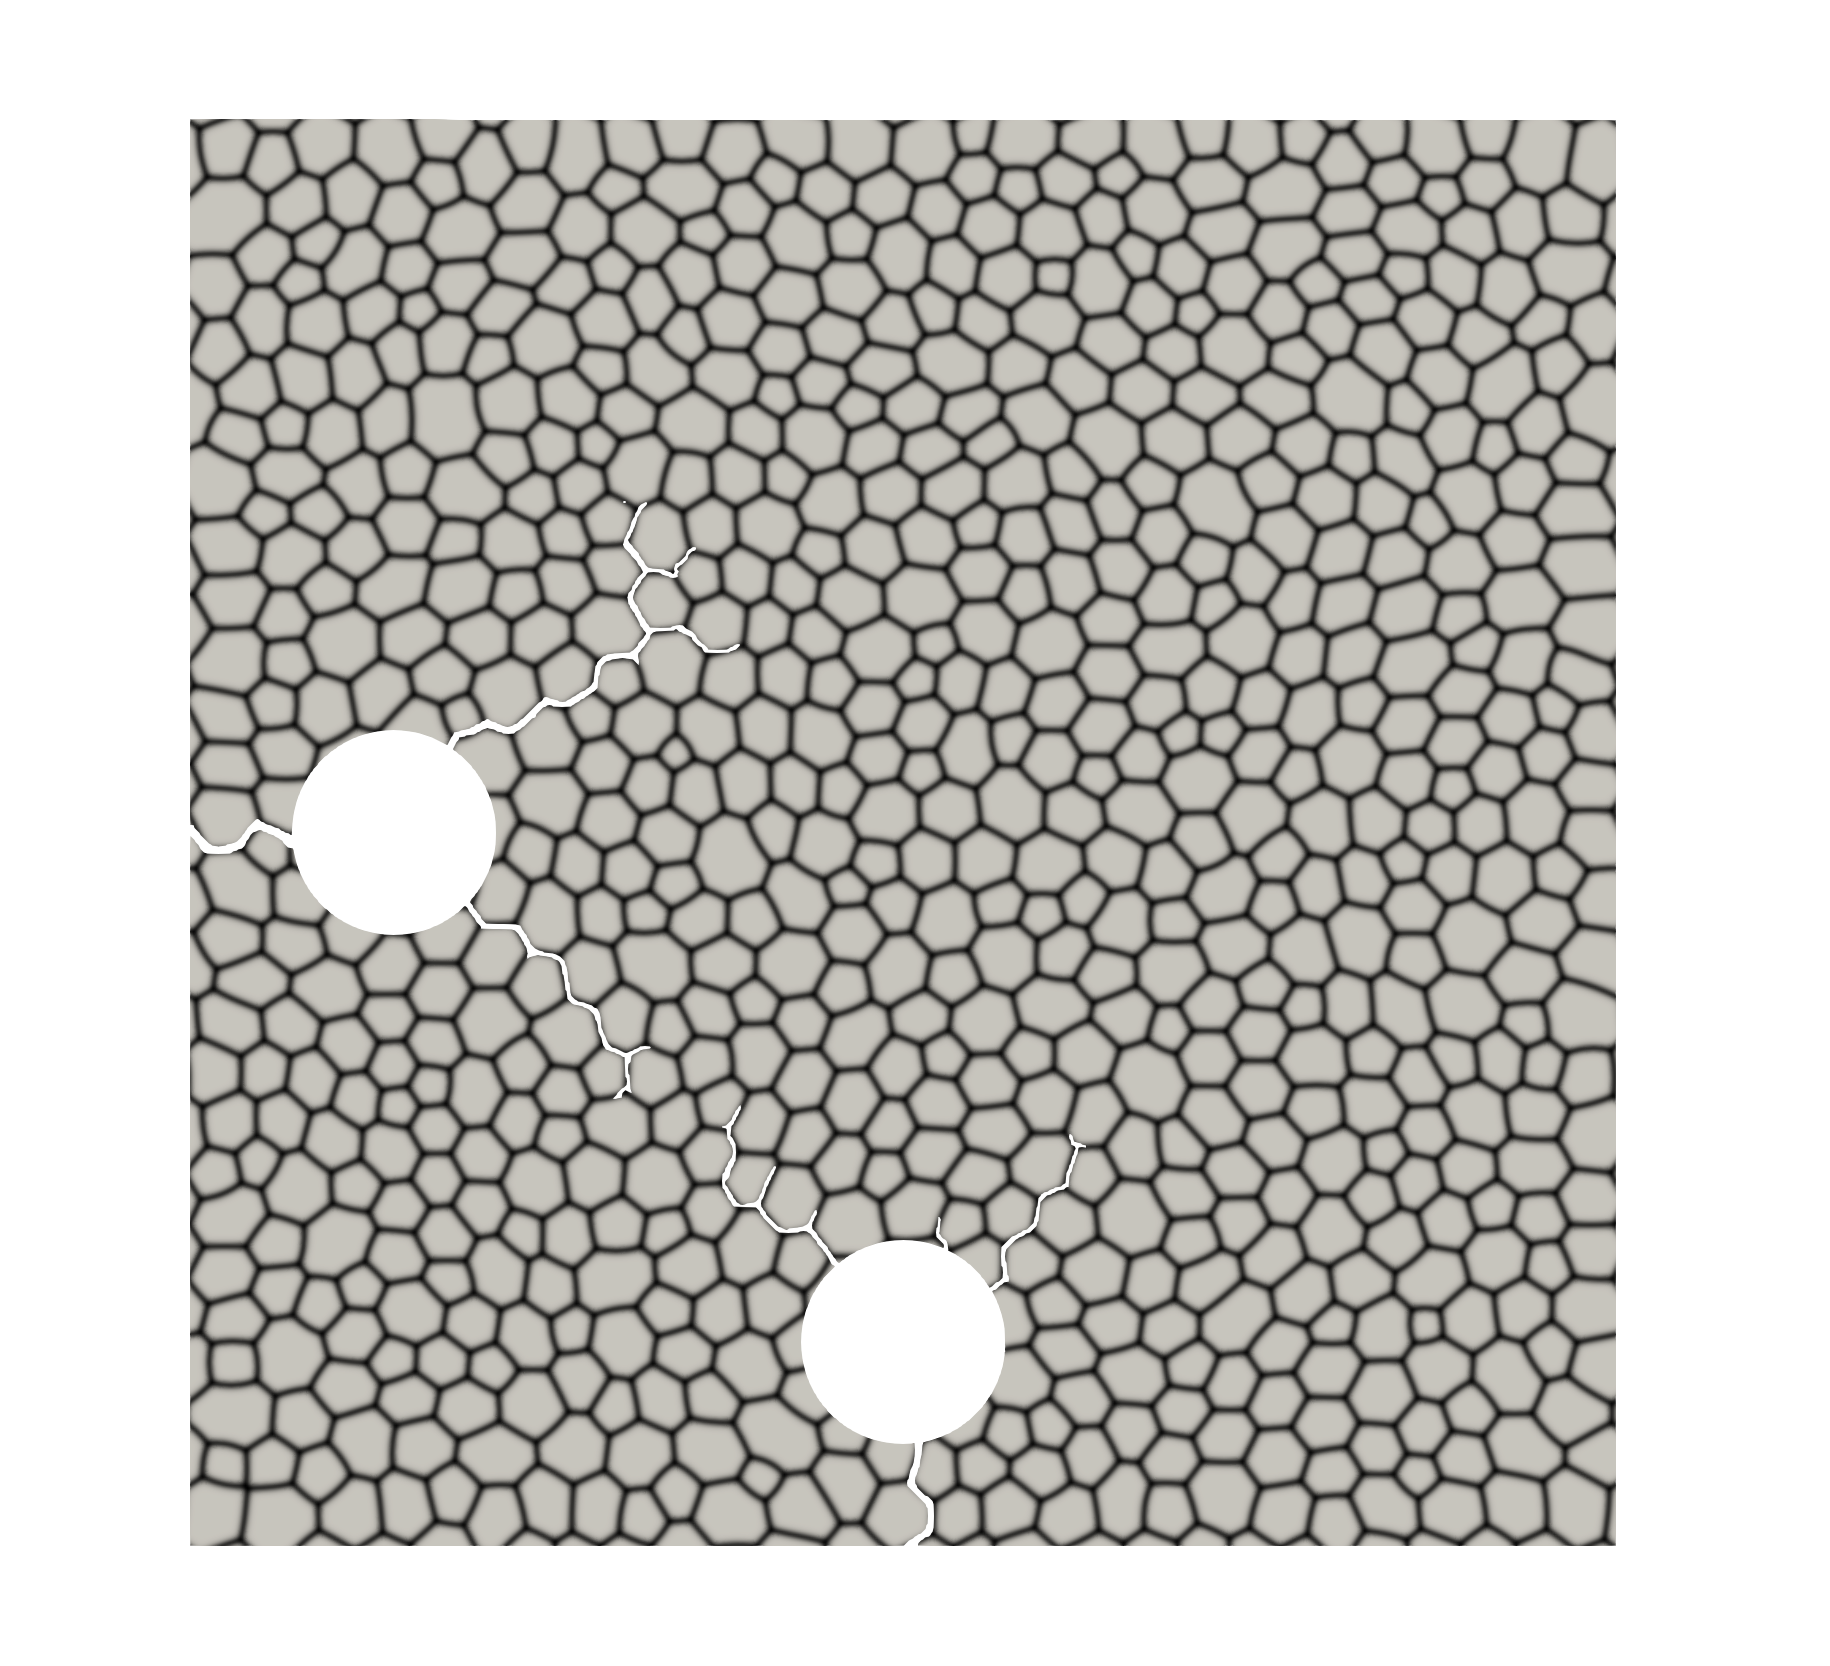
\includegraphics[width=\linewidth]{Chapter3/figures/two_bubbles_bnd}
    \caption{}
  \end{subfigure}
  \begin{subfigure}[t]{0.4\linewidth}
    \centering
    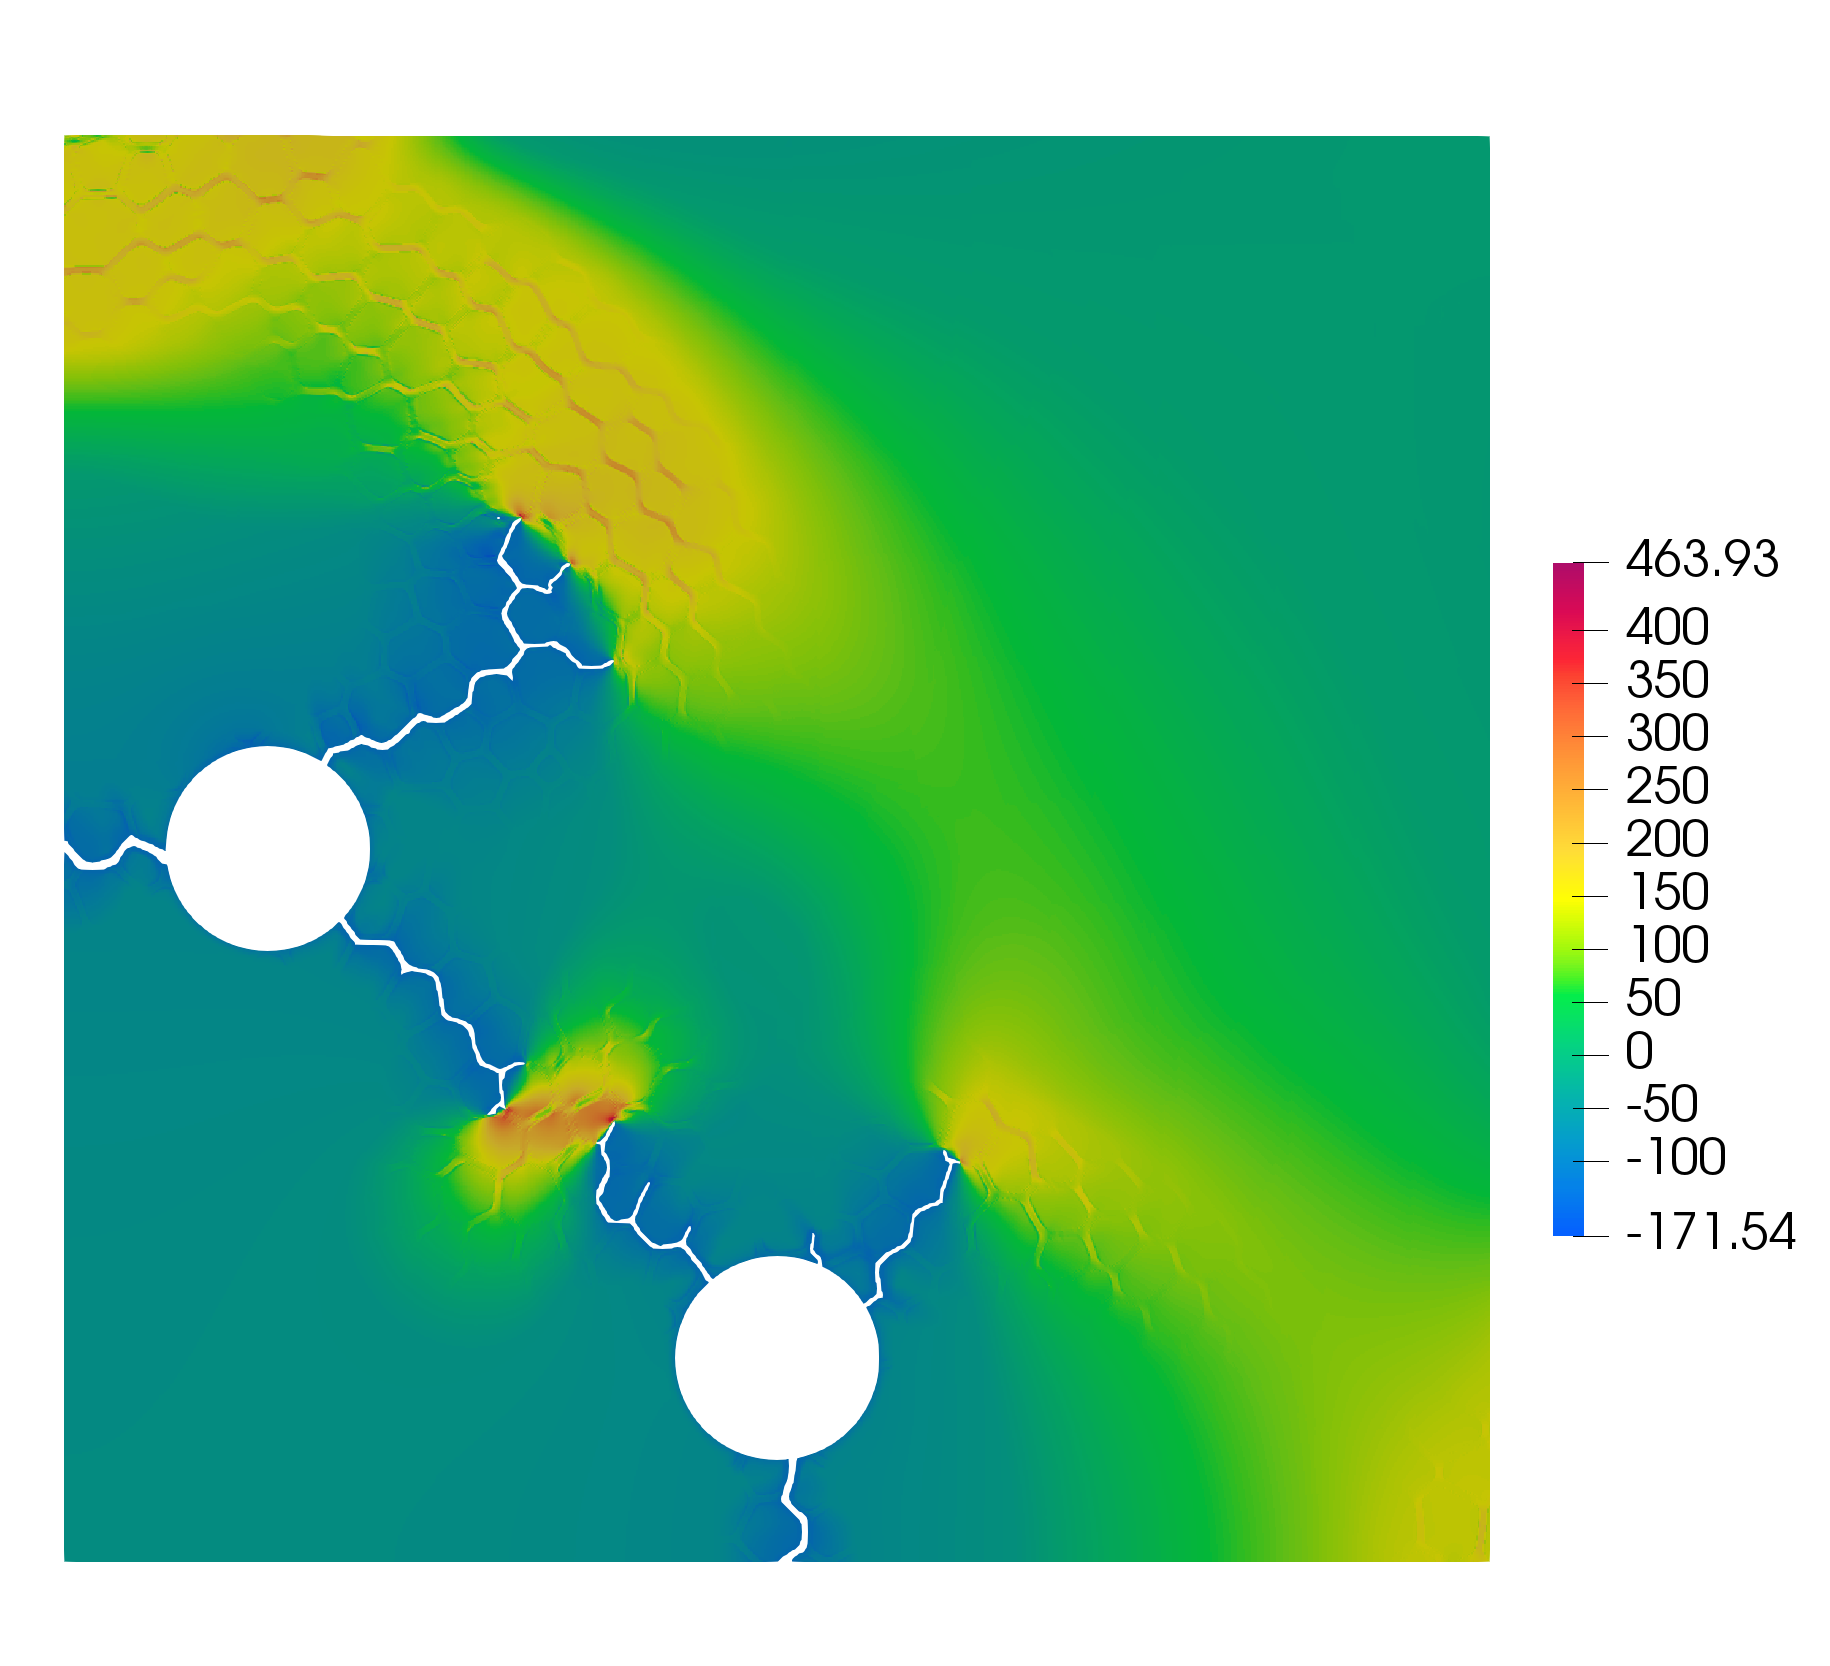
\includegraphics[width=\linewidth]{Chapter3/figures/two_bubbles_stress}
    \caption{}
  \end{subfigure} \\
  \begin{subfigure}[t]{0.4\linewidth}
    \centering
    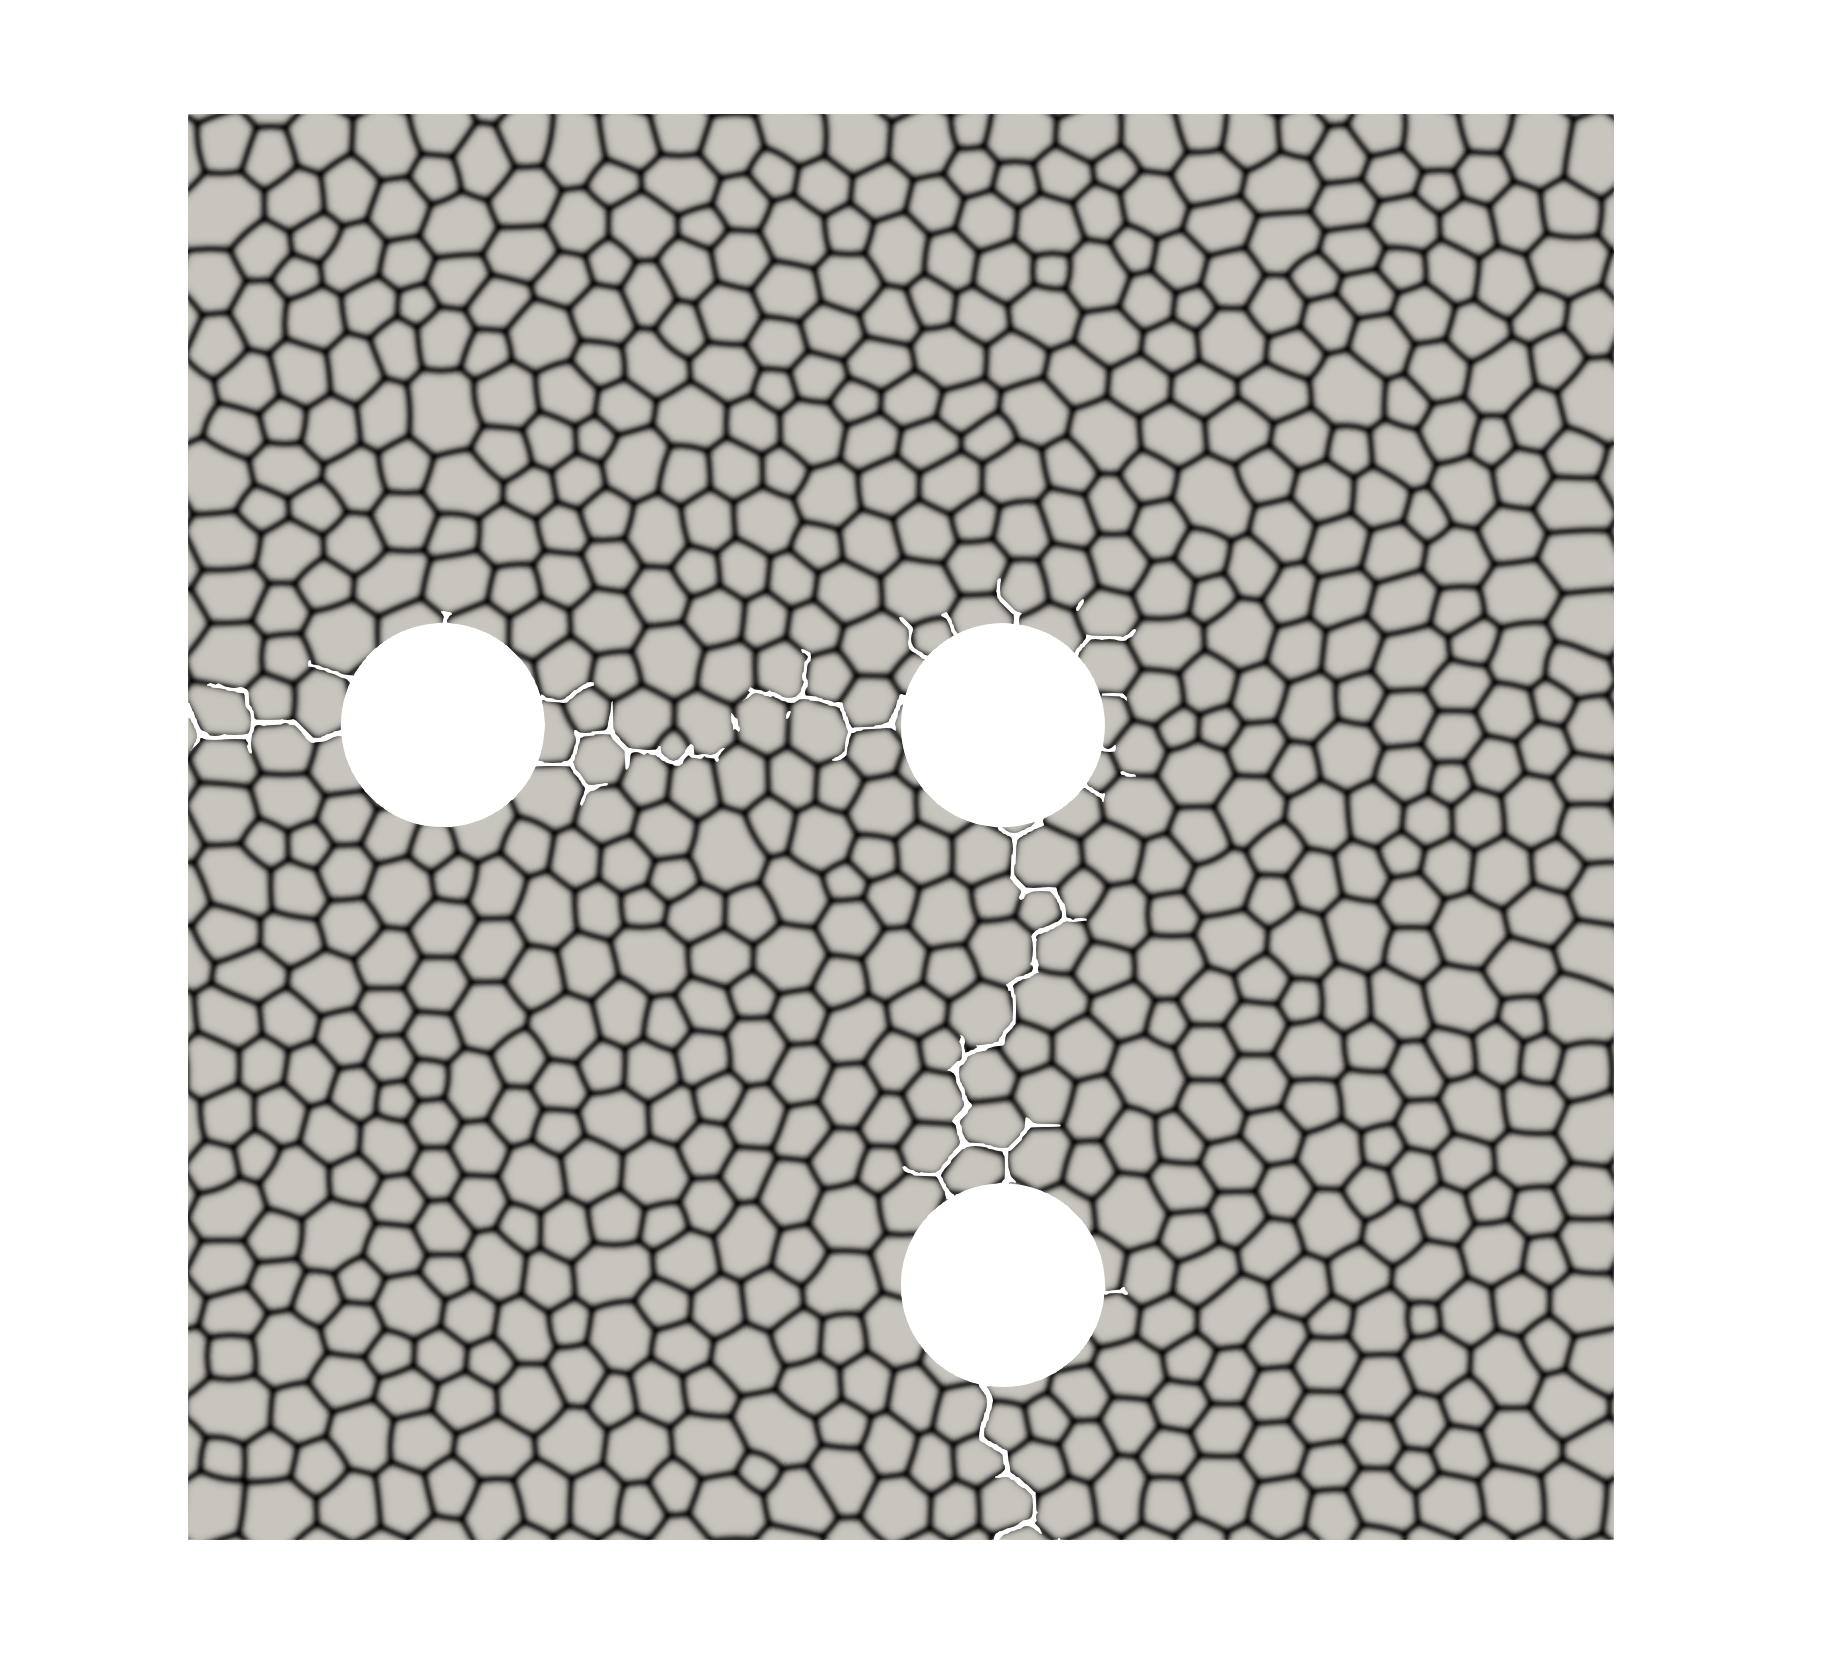
\includegraphics[width=\linewidth]{Chapter3/figures/three_bubbles_bnd}
    \caption{}
  \end{subfigure}
  \begin{subfigure}[t]{0.4\linewidth}
    \centering
    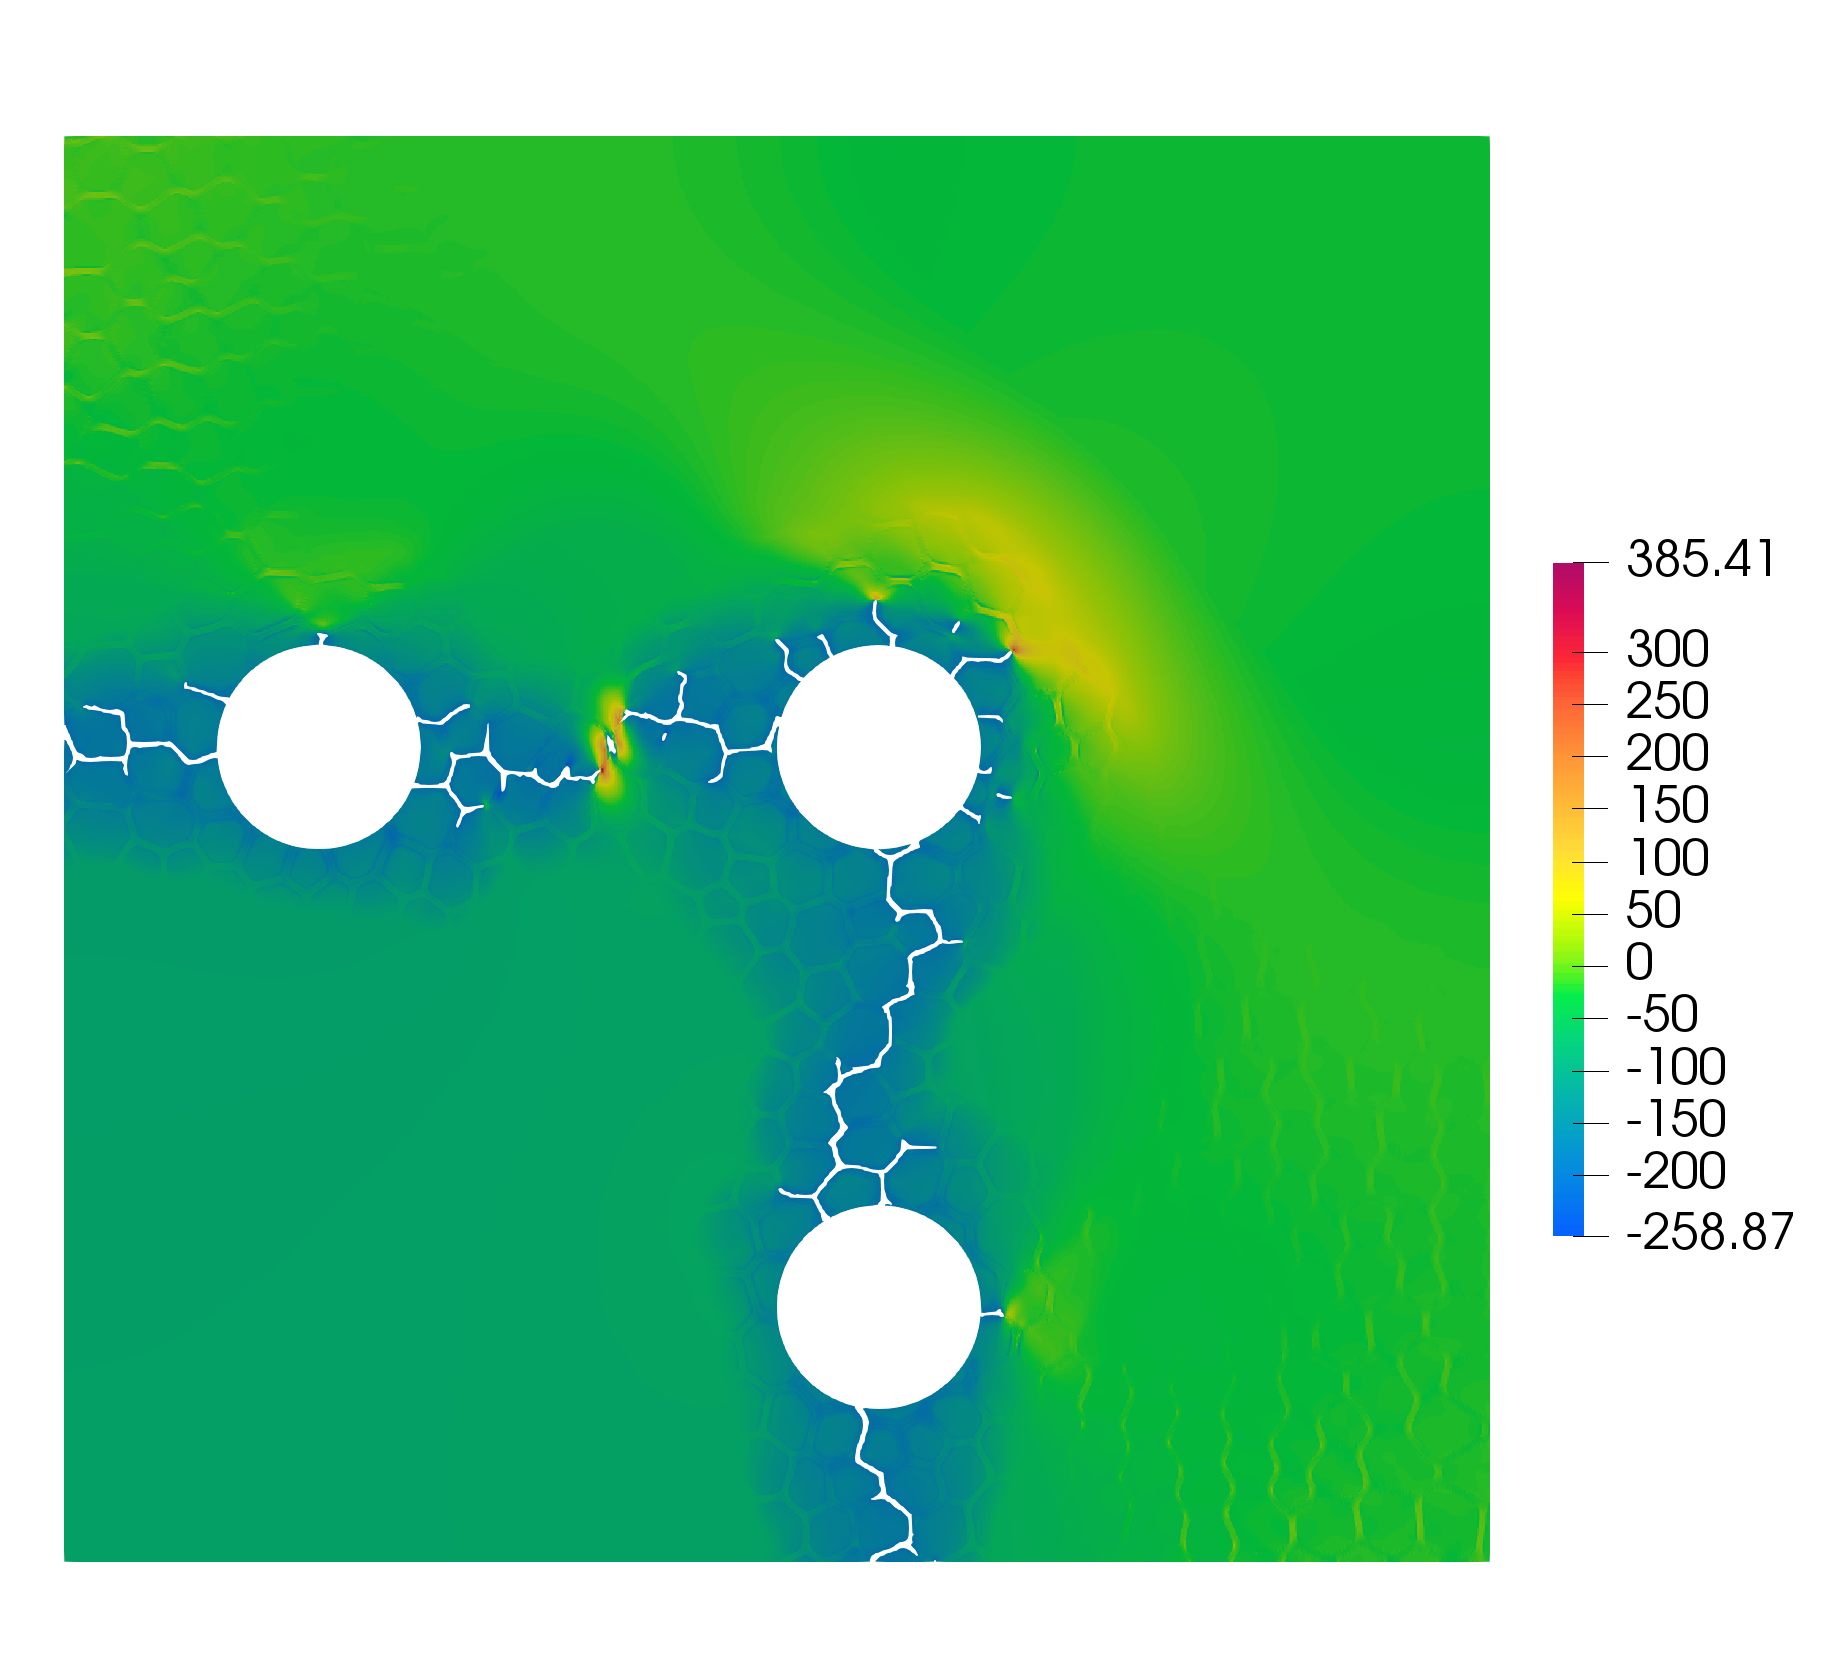
\includegraphics[width=\linewidth]{Chapter3/figures/three_bubbles_stress}
    \caption{}
  \end{subfigure}
  \caption[Crack propagation from multiple bubbles.]{Results for (a-b) the two-bubble case and (c-d) the three-bubble case. (a, c) Crack paths superimposed on the voronoi structure. (b, d) Contour plot of the maximum principal stress.}
  \label{fig:compare_bubble_distribution}
\end{figure}

%%%%%%%%%%%%%%%%%%%%%%%%%%%%%%%%%%%%%%%%%%%%%%%%%%%%%%%%%%%%%%%%%%%%%%%%%%%%%%%%%%%%%%%%%%%
%%%%%%%%%%%%%%%%%%%%%%%%%%%%%%%%%%%%%%%%%%%%%%%%%%%%%%%%%%%%%%%%%%%%%%%%%%%%%%%%%%%%%%%%%%%
%%%%%%%%%%%%%%%%%%%%%%%%%%%%%%%%%%%%%%%%%%%%%%%%%%%%%%%%%%%%%%%%%%%%%%%%%%%%%%%%%%%%%%%%%%%
%%%%%%%%%%%%%%%%%%%%%%%%%%%%%%%%%%%%%%%%%%%%%%%%%%%%%%%%%%%%%%%%%%%%%%%%%%%%%%%%%%%%%%%%%%%
%%%%%%%%%%%%%%%%%%%%%%%%%%%%%%%%%%%%%%%%%%%%%%%%%%%%%%%%%%%%%%%%%%%%%%%%%%%%%%%%%%%%%%%%%%%
%%%%%%%%%%%%%%%%%%%%%%%%%%%%%%%%%%%%%%%%%%%%%%%%%%%%%%%%%%%%%%%%%%%%%%%%%%%%%%%%%%%%%%%%%%%
%%%%%%%%%%%%%%%%%%%%%%%%%%%%%%%%%%%%%%%%%%%%%%%%%%%%%%%%%%%%%%%%%%%%%%%%%%%%%%%%%%%%%%%%%%%
%%%%%%%%%%%%%%%%%%%%%%%%%%%%%%%%%%%%%%%%%%%%%%%%%%%%%%%%%%%%%%%%%%%%%%%%%%%%%%%%%%%%%%%%%%%
%%%%%%%%%%%%%%%%%%%%%%%%%%%%%%%%%%%%%%%%%%%%%%%%%%%%%%%%%%%%%%%%%%%%%%%%%%%%%%%%%%%%%%%%%%%
%%%%%%%%%%%%%%%%%%%%%%%%%%%%%%%%%%%%%%%%%%%%%%%%%%%%%%%%%%%%%%%%%%%%%%%%%%%%%%%%%%%%%%%%%%%
\subsubsection{Partial HBS}

Lastly, we incorporate defect evolution and recrystallization into the quasi-brittle fracture model. A phase-field model is used to simulate the defect evolution and the recrystallization behavior leading to HBS formation. A detailed description of the phase-field model is available in \cite{Aagesen2020}. The quasi-brittle fracture model is applied directly on the microstructure resulting from simulations of the HBS formation process. Considering the fact that fragmentation can be observed in partially recrystallized zones, we focus on the fracture behavior of partial HBS.
Three HBS at different recrystallization stages with $25\%$, $60\%$, and $100\%$ recrystallization fraction are considered. A linearly increasing gas pressure is applied. Results are shown in \Cref{fig:partial_hbs}. In all three cases, cracks nucleate at around 60 MPa, owing to their similar defect sizes. Crack nucleation locations vary among the three cases, as more grains form around the defect during recrystallization and their intersections with the defect become possible nucleation sites. Furthermore, recrystallization changes the grain morphology, leading to different crack paths.

\begin{figure}[htb!]
  \centering
  \begin{subfigure}[t]{0.4\linewidth}
    \centering
    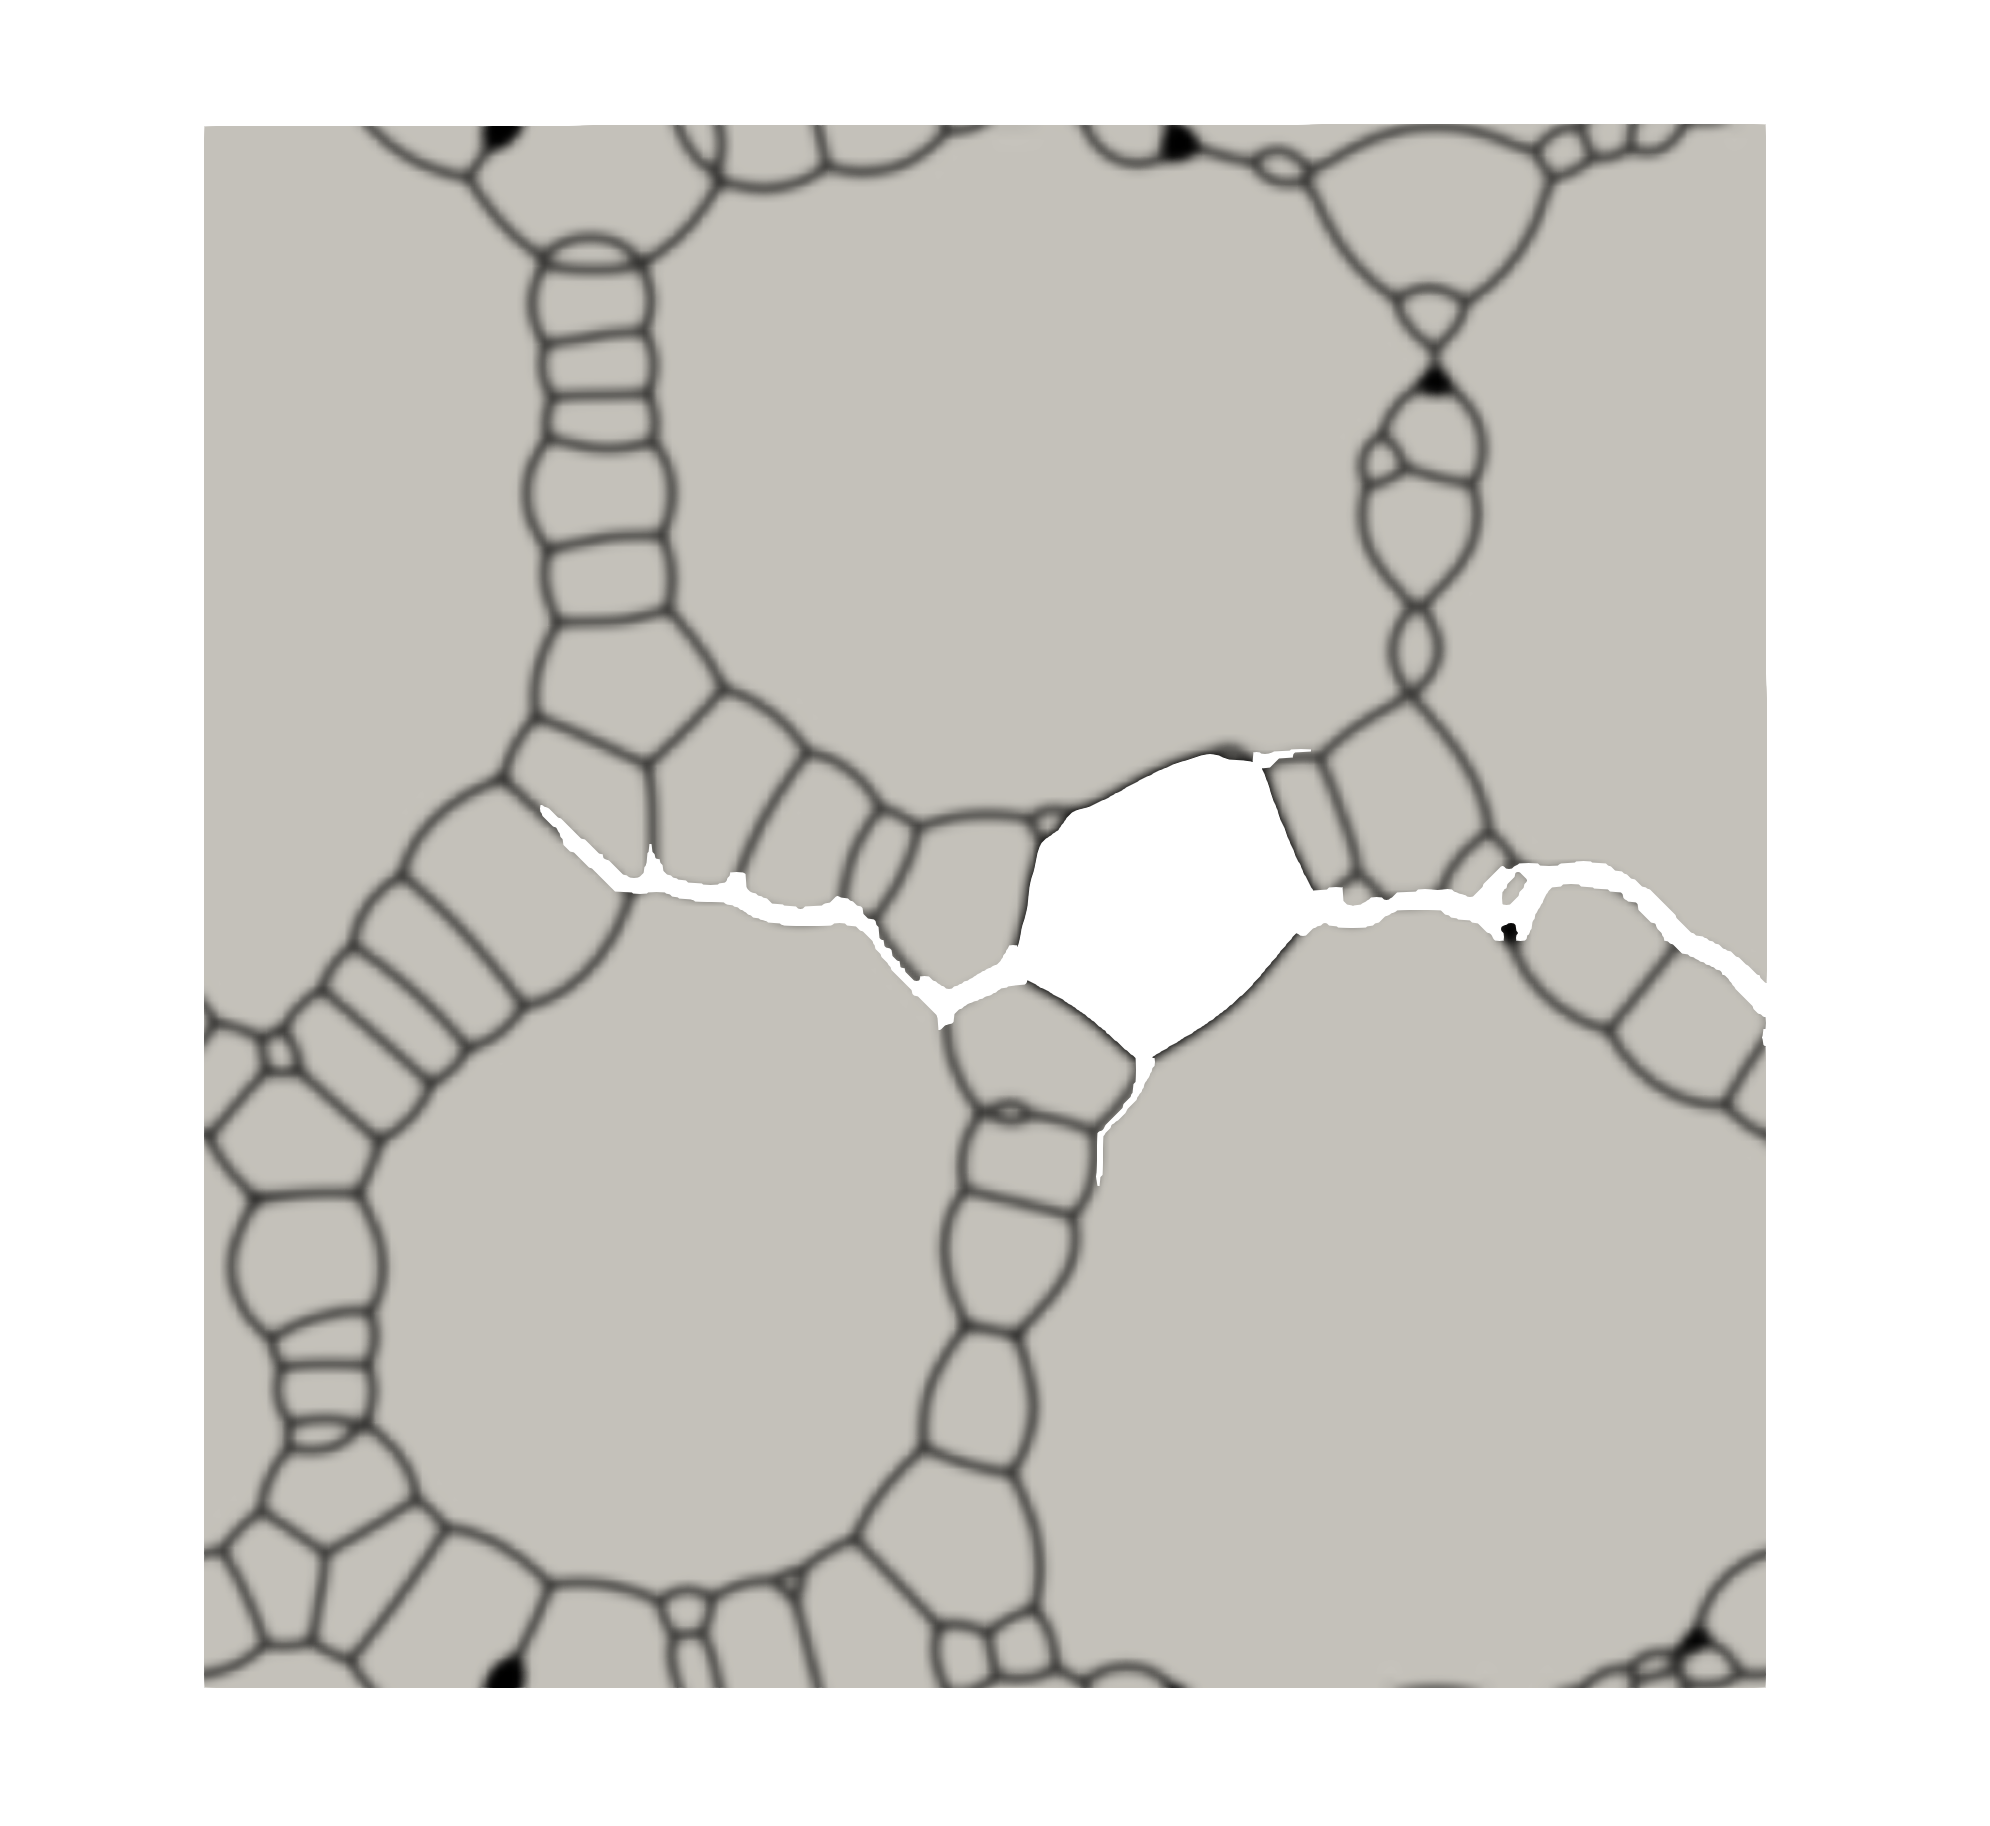
\includegraphics[width=\linewidth]{Chapter3/figures/partial_hbs_1}
    \caption{}
  \end{subfigure}
  \begin{subfigure}[t]{0.4\linewidth}
    \centering
    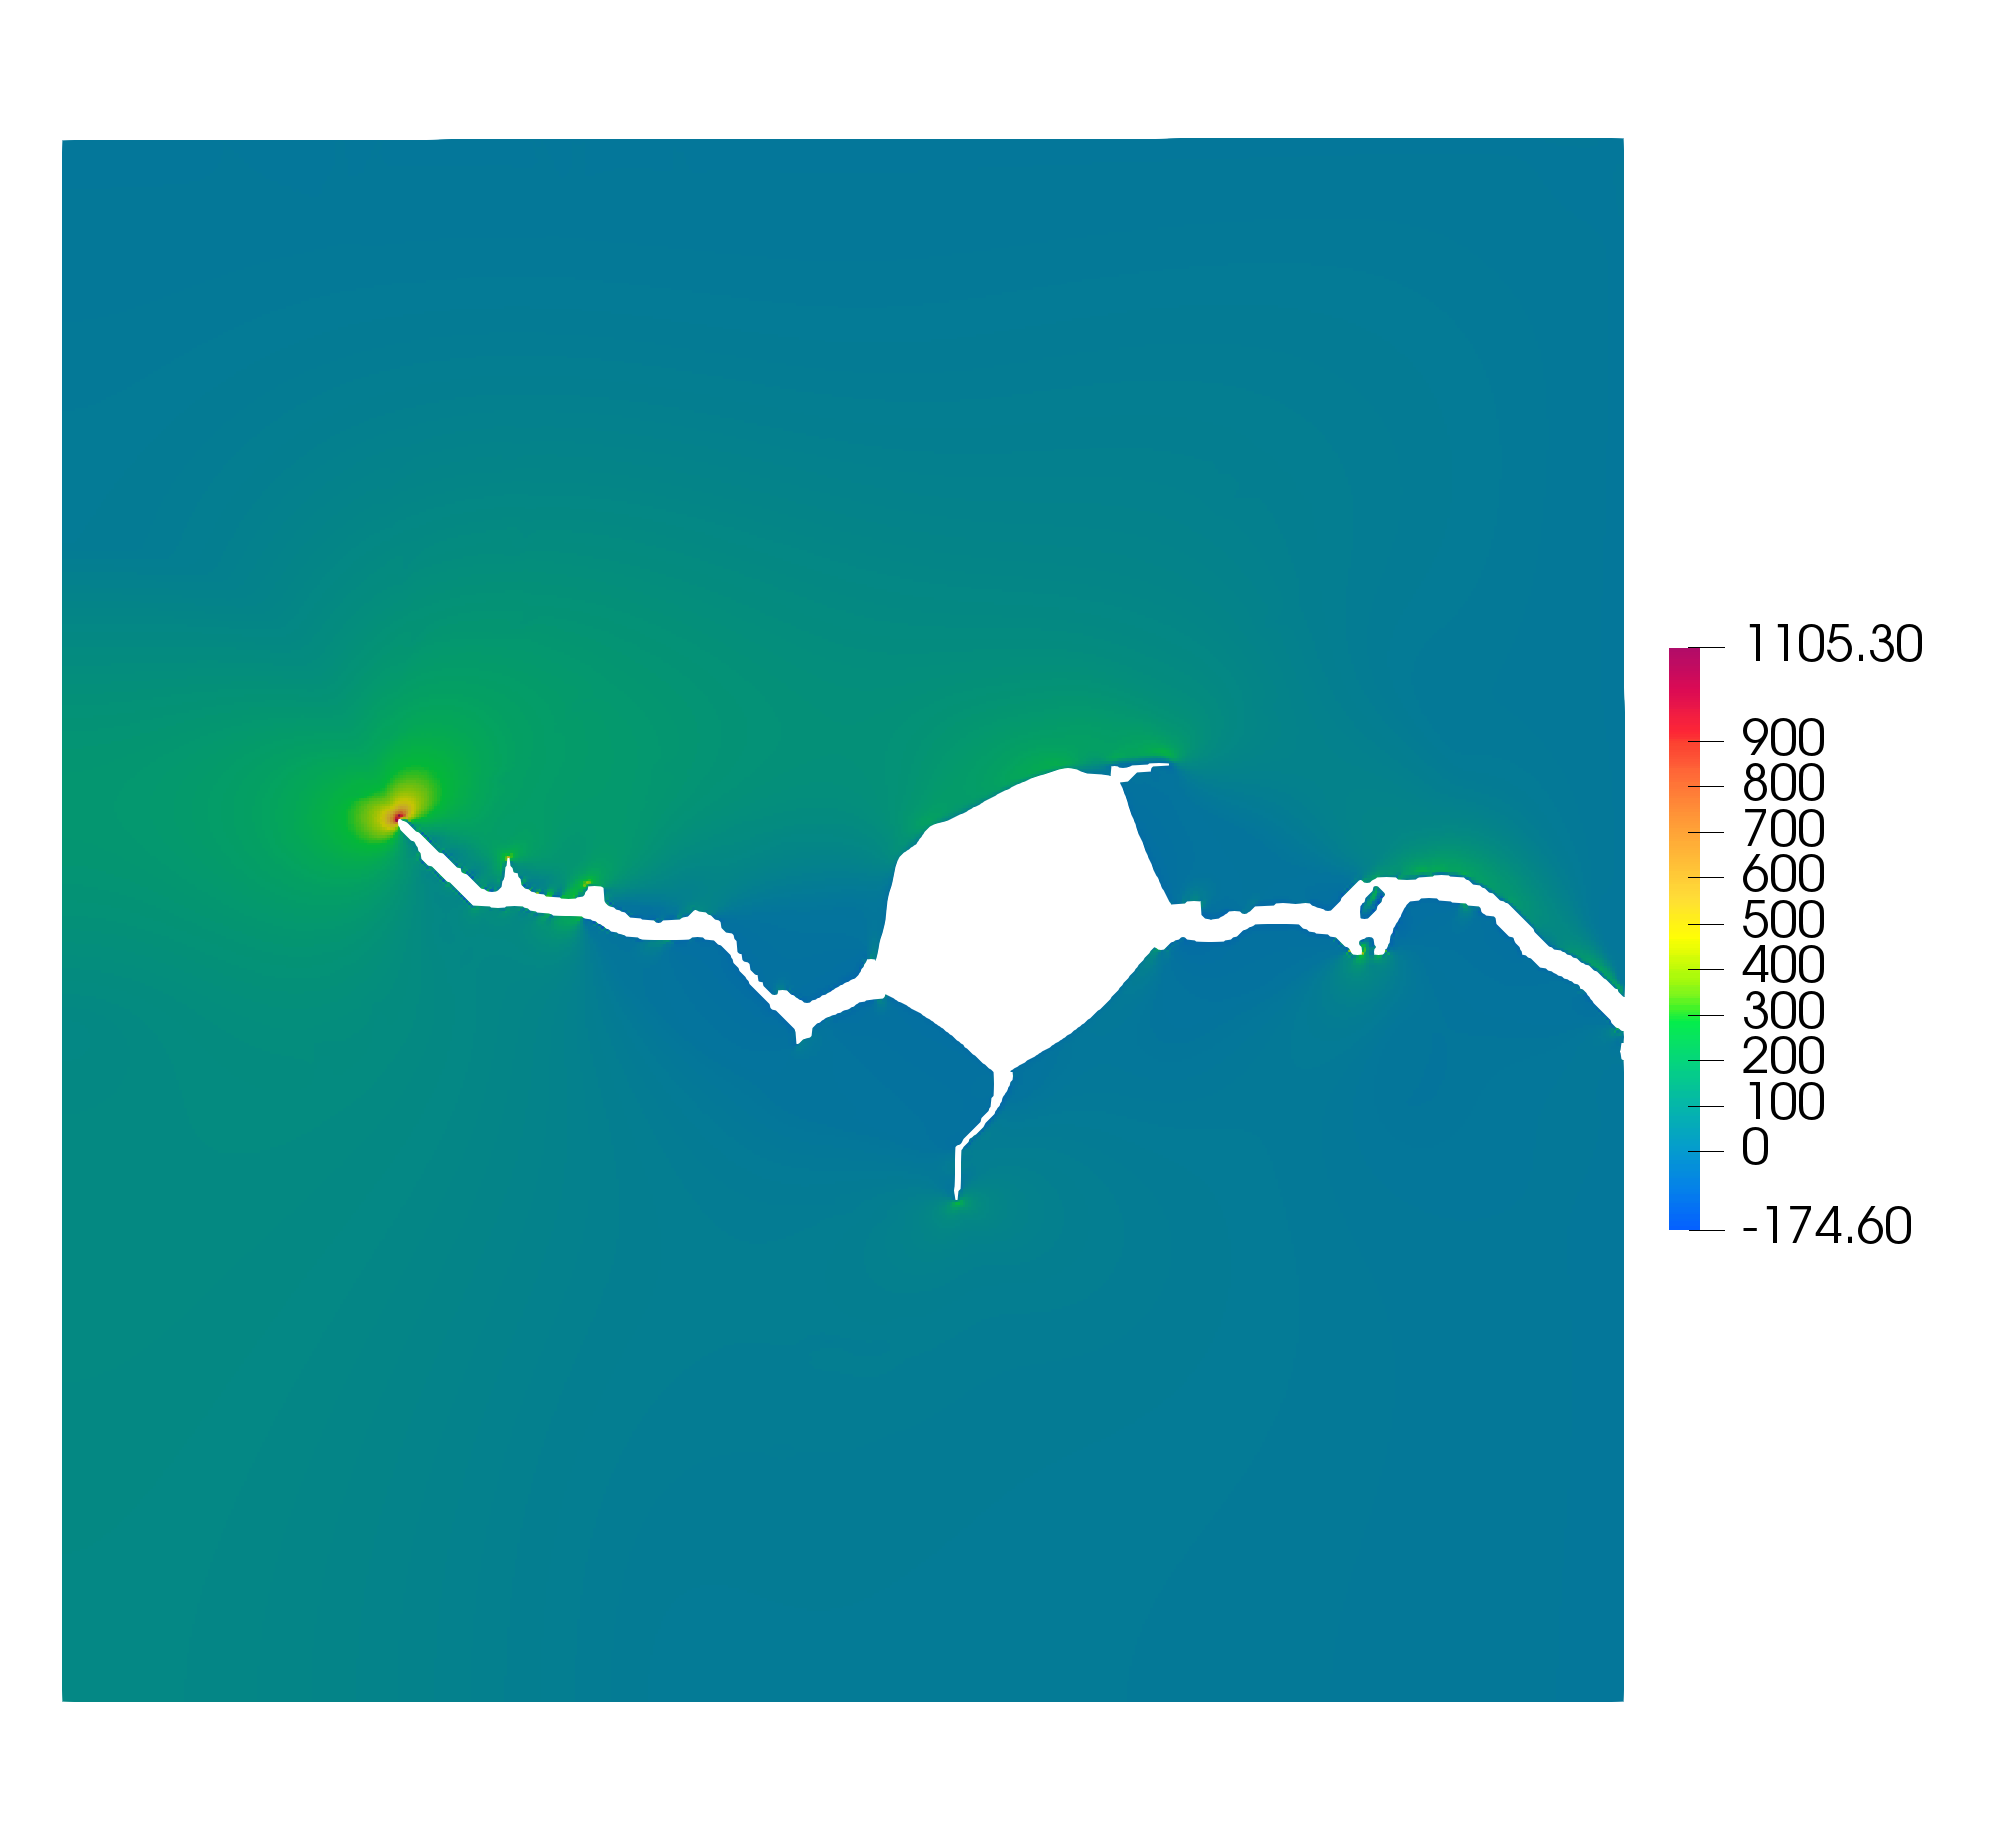
\includegraphics[width=\linewidth]{Chapter3/figures/partial_hbs_1_stress}
    \caption{}
  \end{subfigure}\\
  \begin{subfigure}[t]{0.4\linewidth}
    \centering
    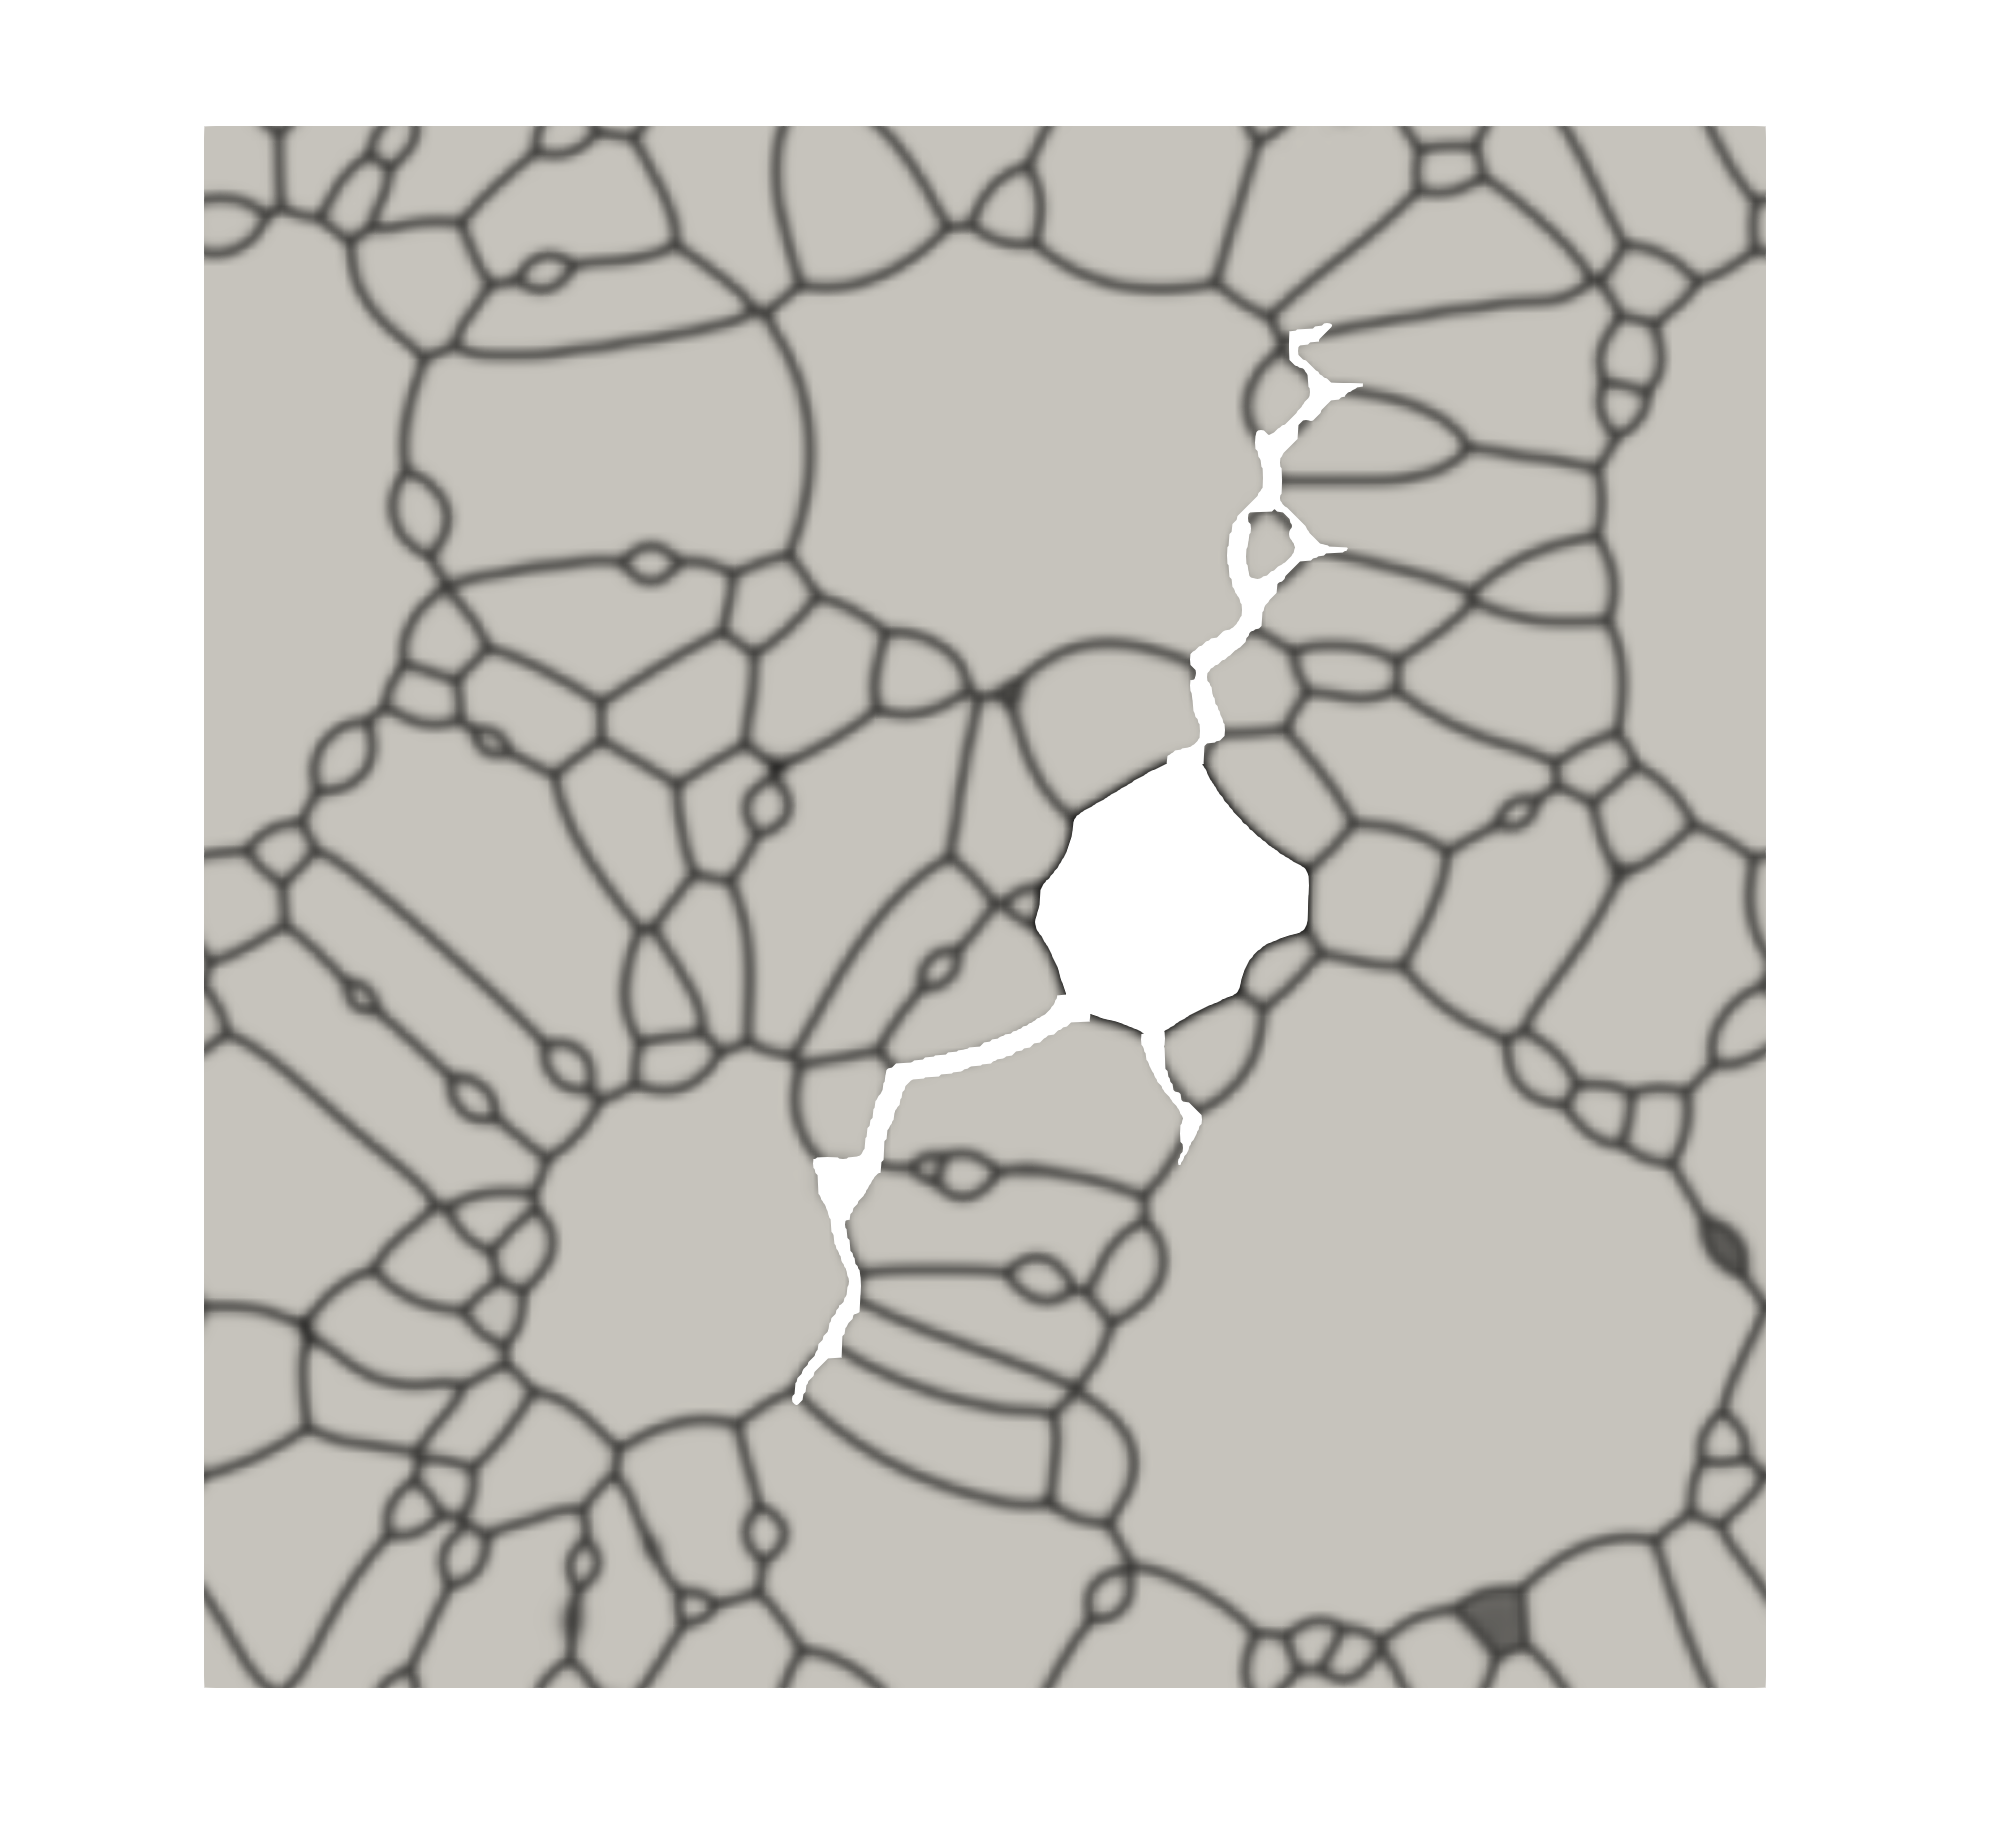
\includegraphics[width=\linewidth]{Chapter3/figures/partial_hbs_2}
    \caption{}
  \end{subfigure}
  \begin{subfigure}[t]{0.4\linewidth}
    \centering
    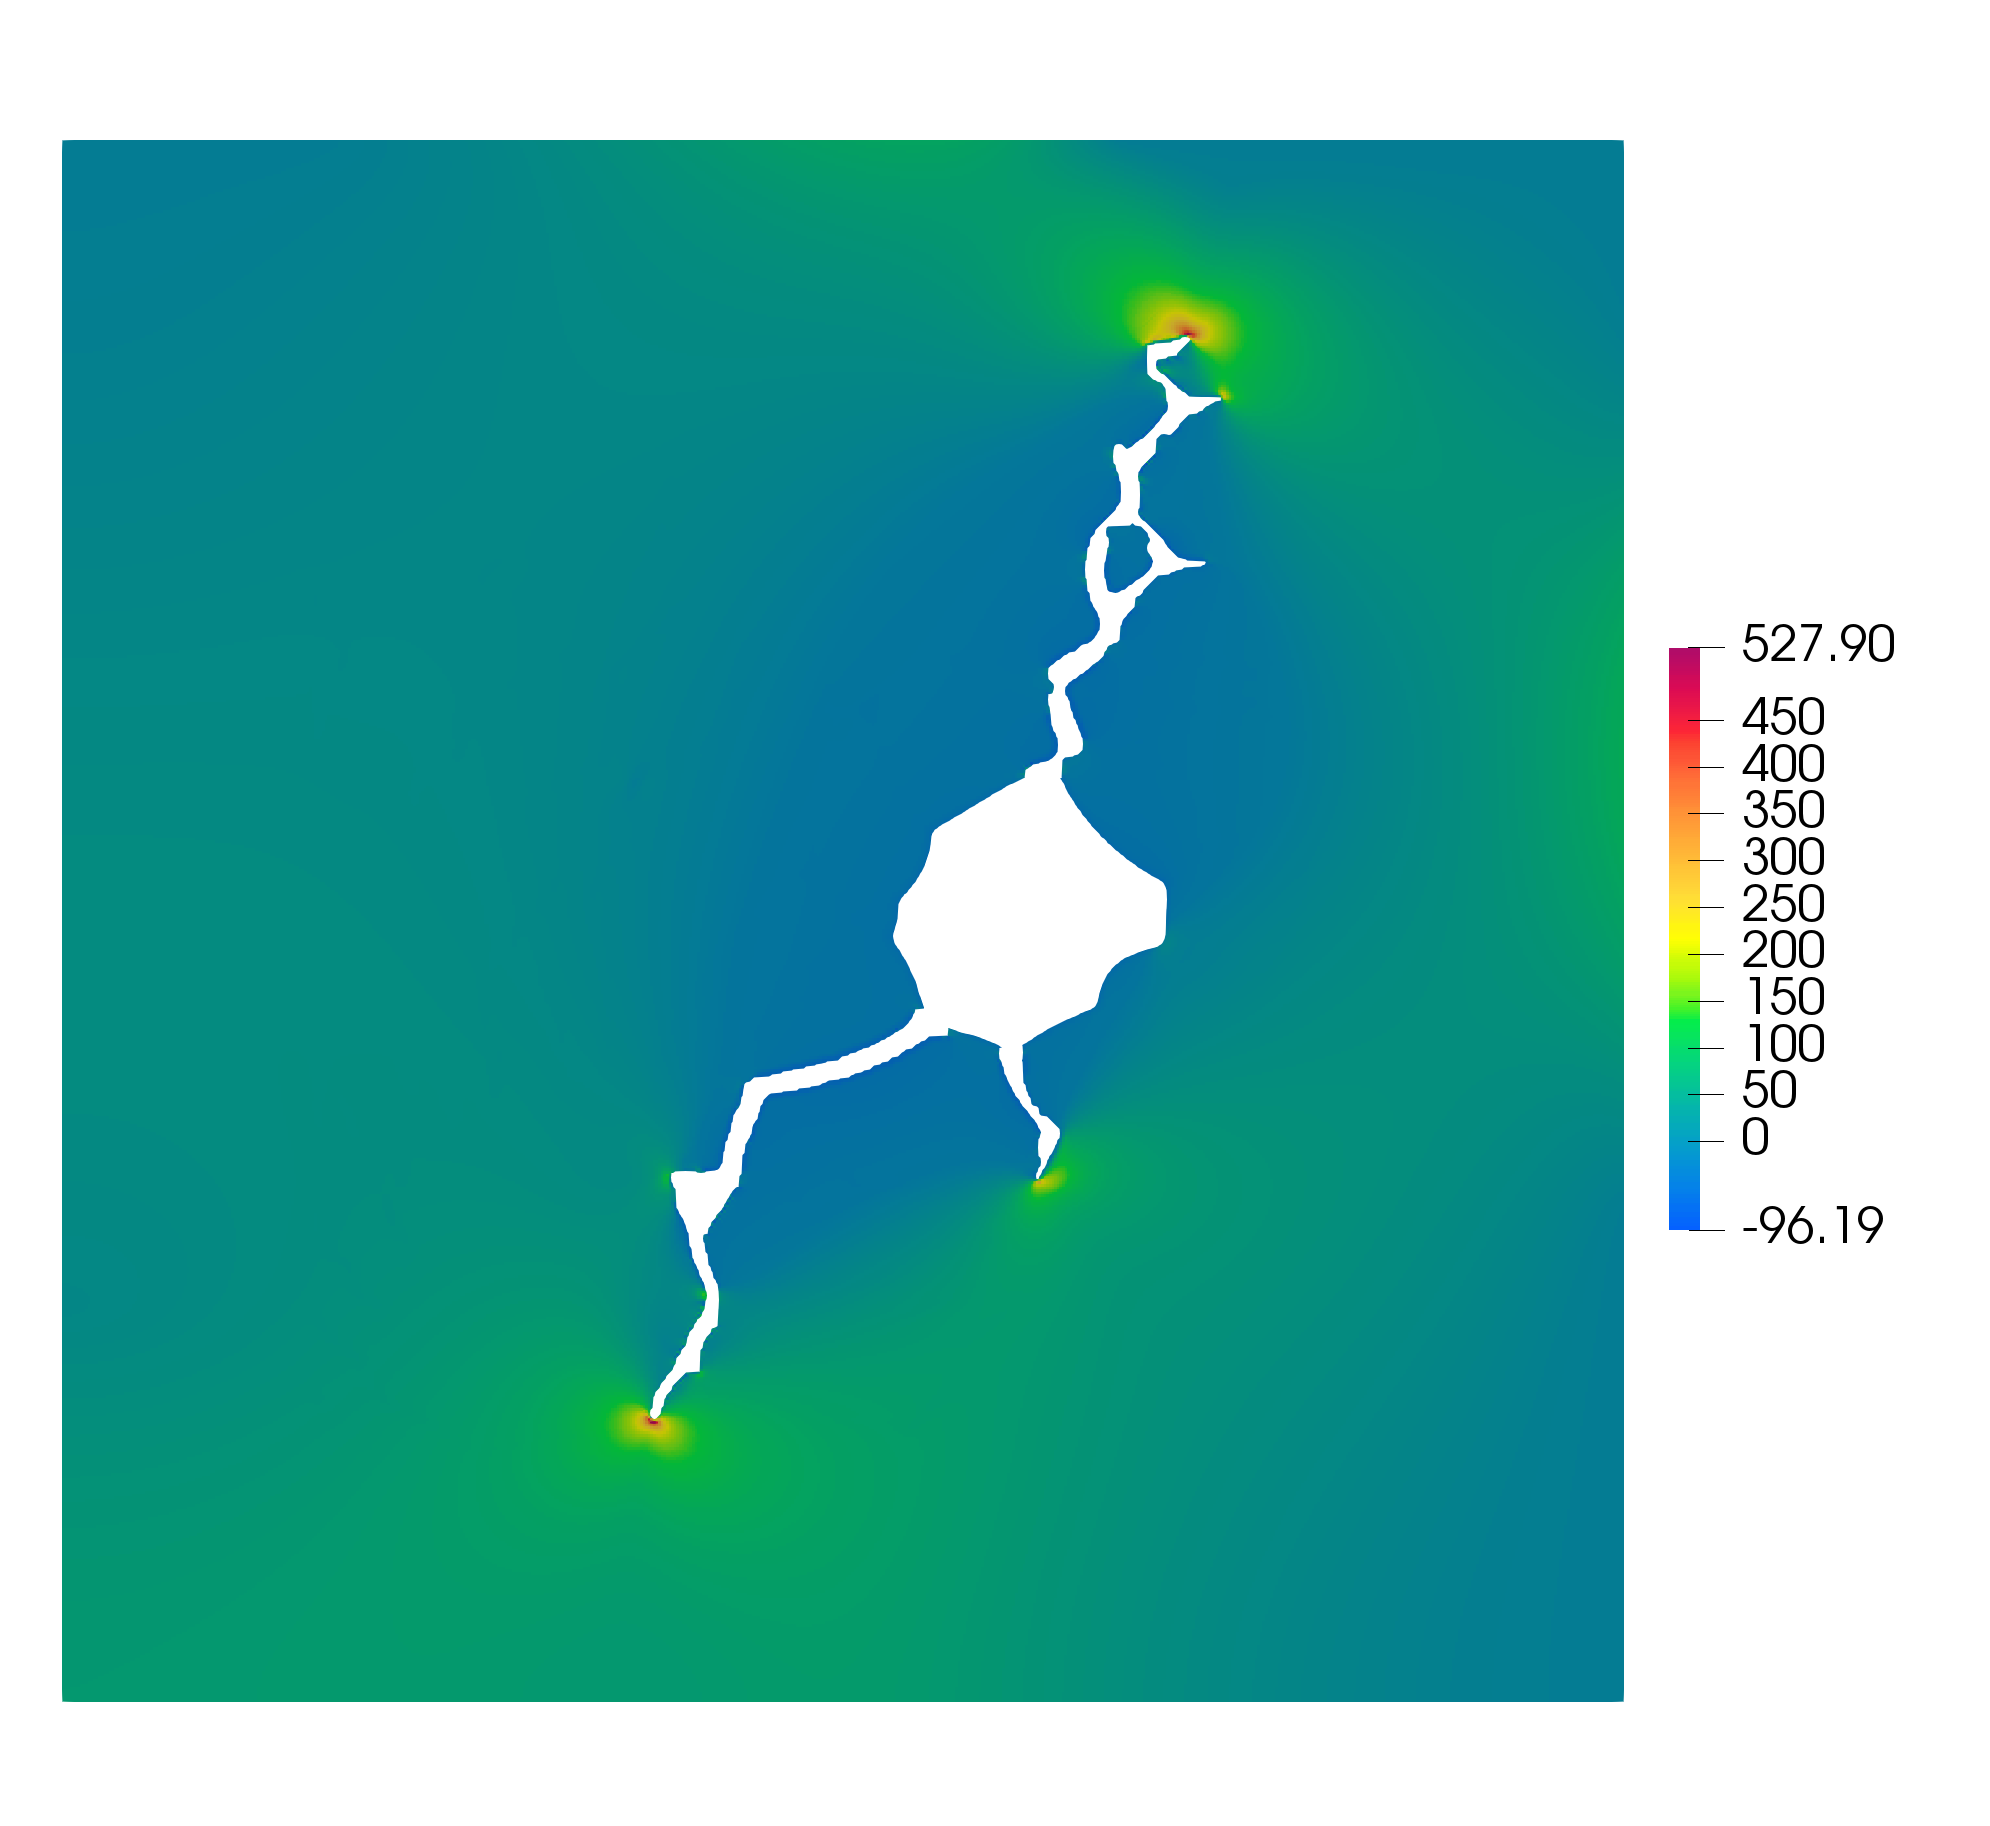
\includegraphics[width=\linewidth]{Chapter3/figures/partial_hbs_2_stress}
    \caption{}
  \end{subfigure}\\
  \begin{subfigure}[t]{0.4\linewidth}
    \centering
    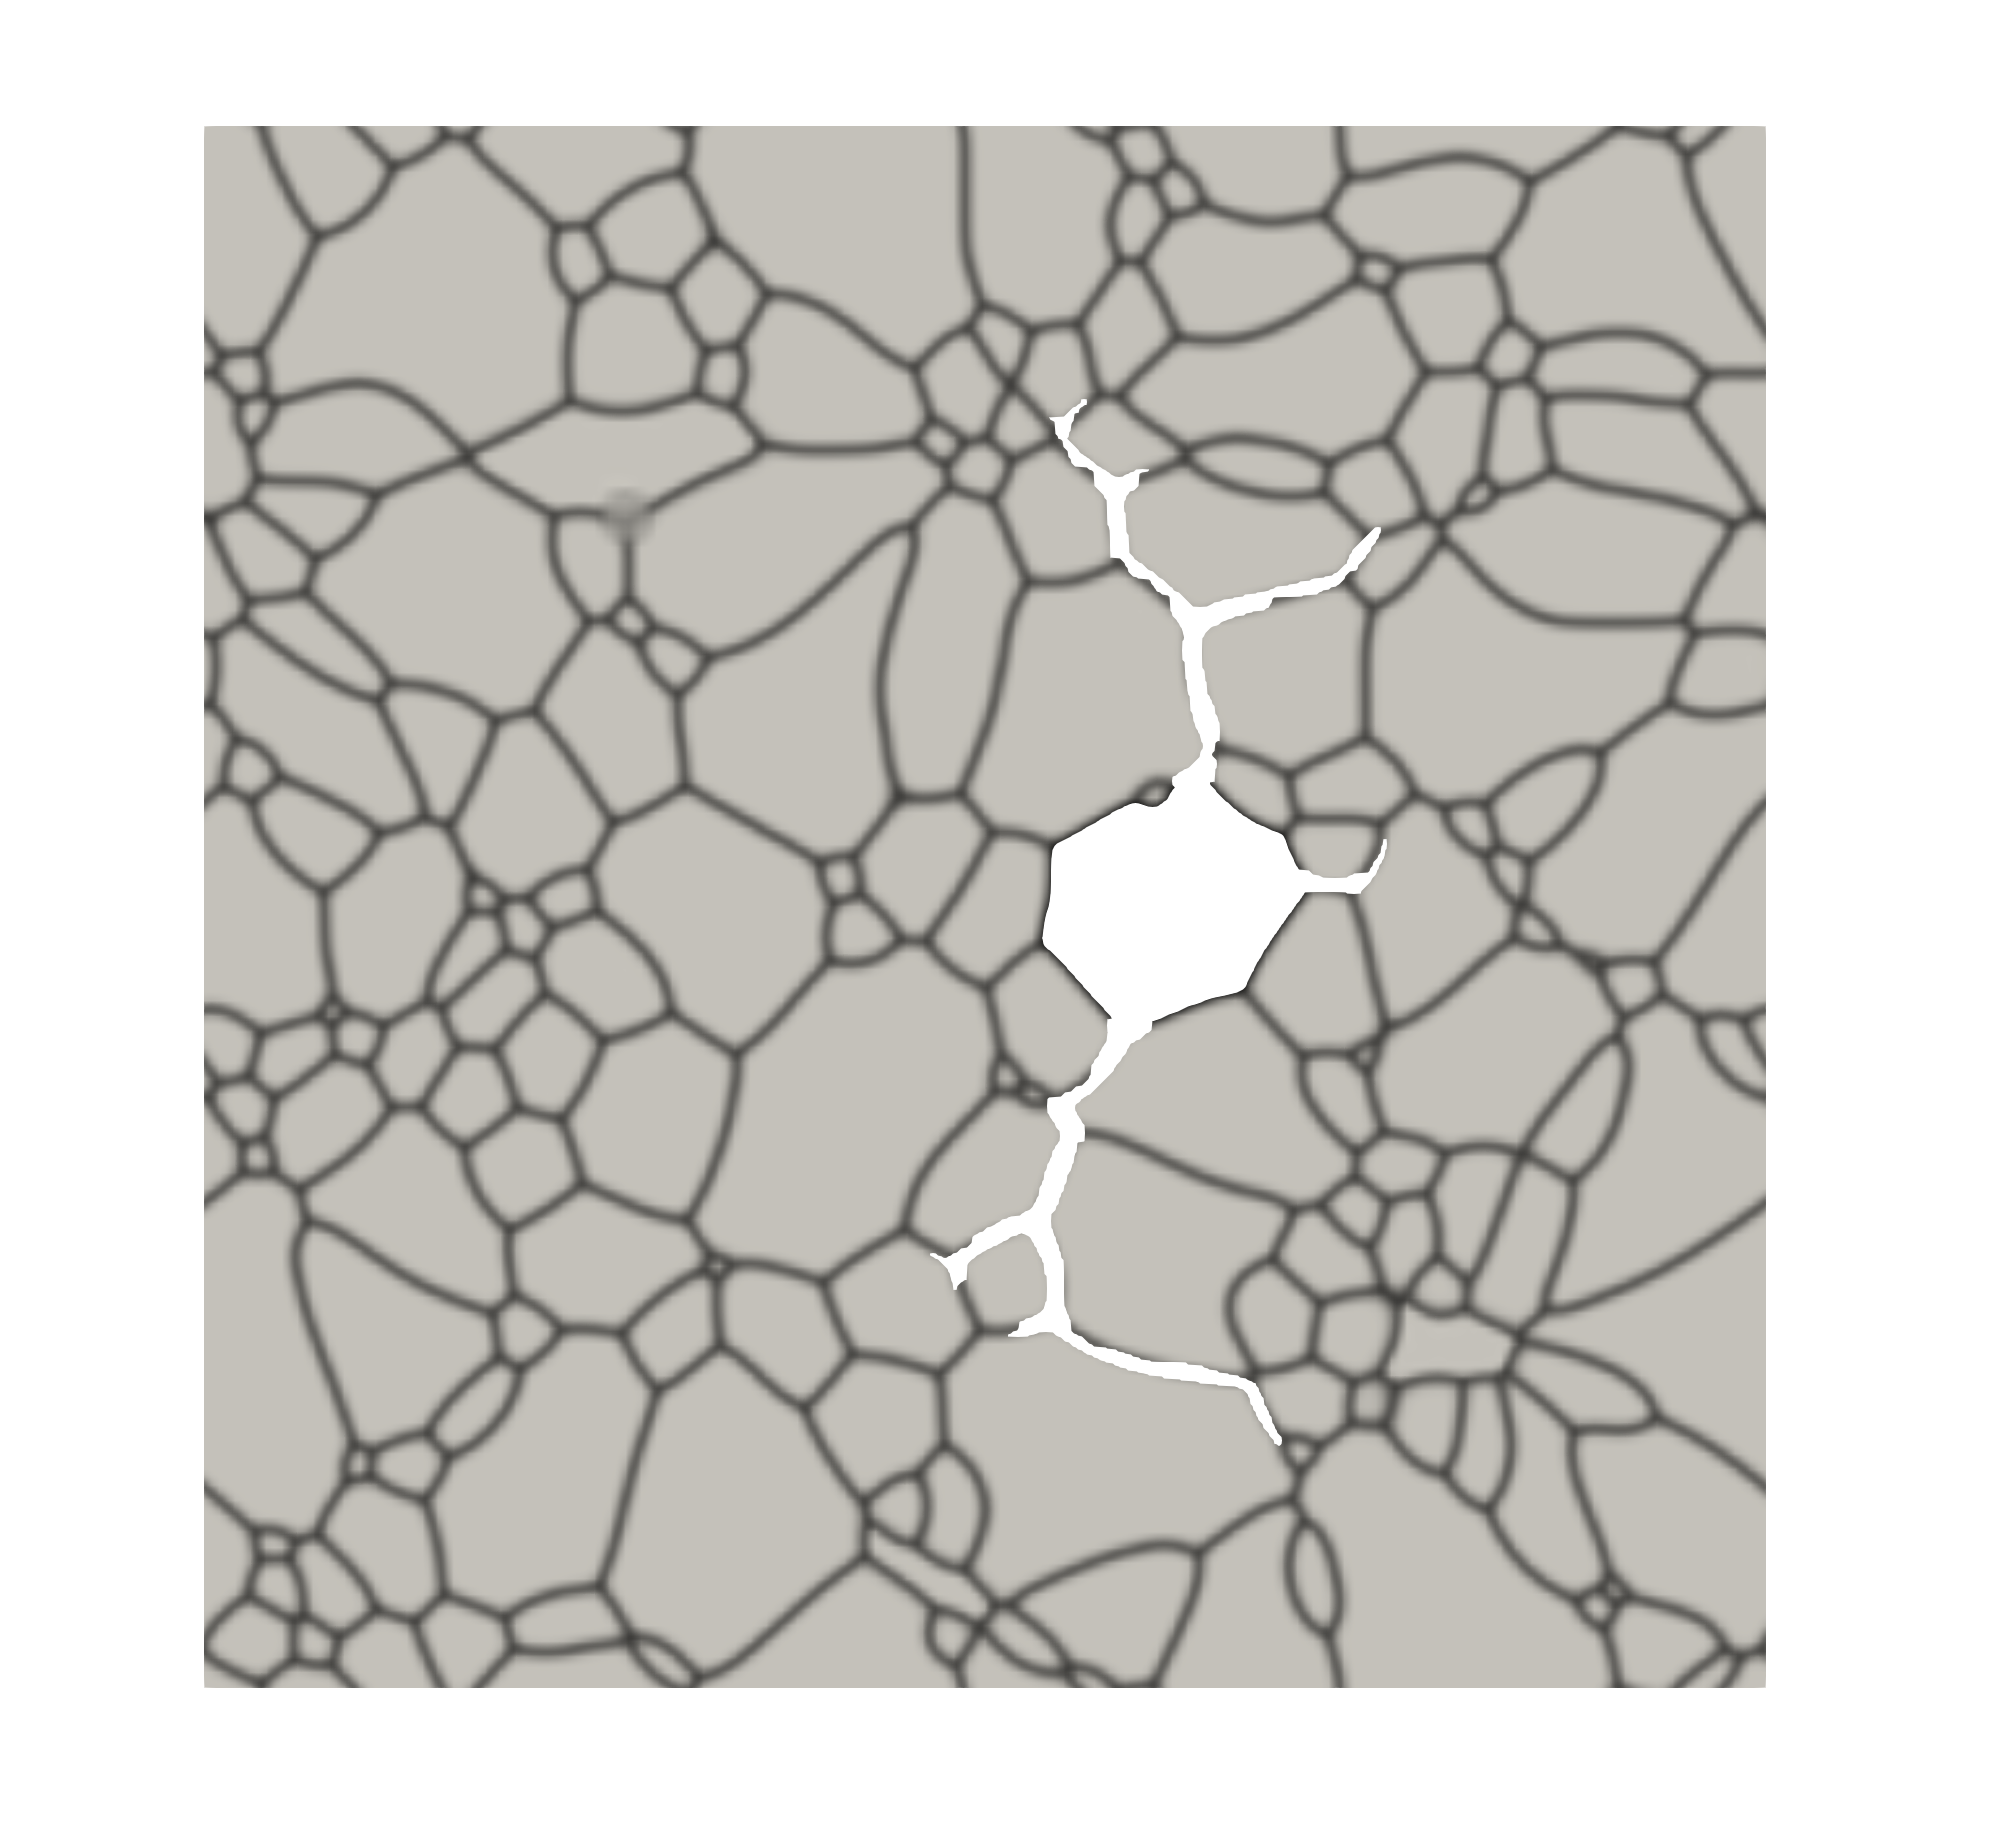
\includegraphics[width=\linewidth]{Chapter3/figures/partial_hbs_3}
    \caption{}
  \end{subfigure}
  \begin{subfigure}[t]{0.4\linewidth}
    \centering
    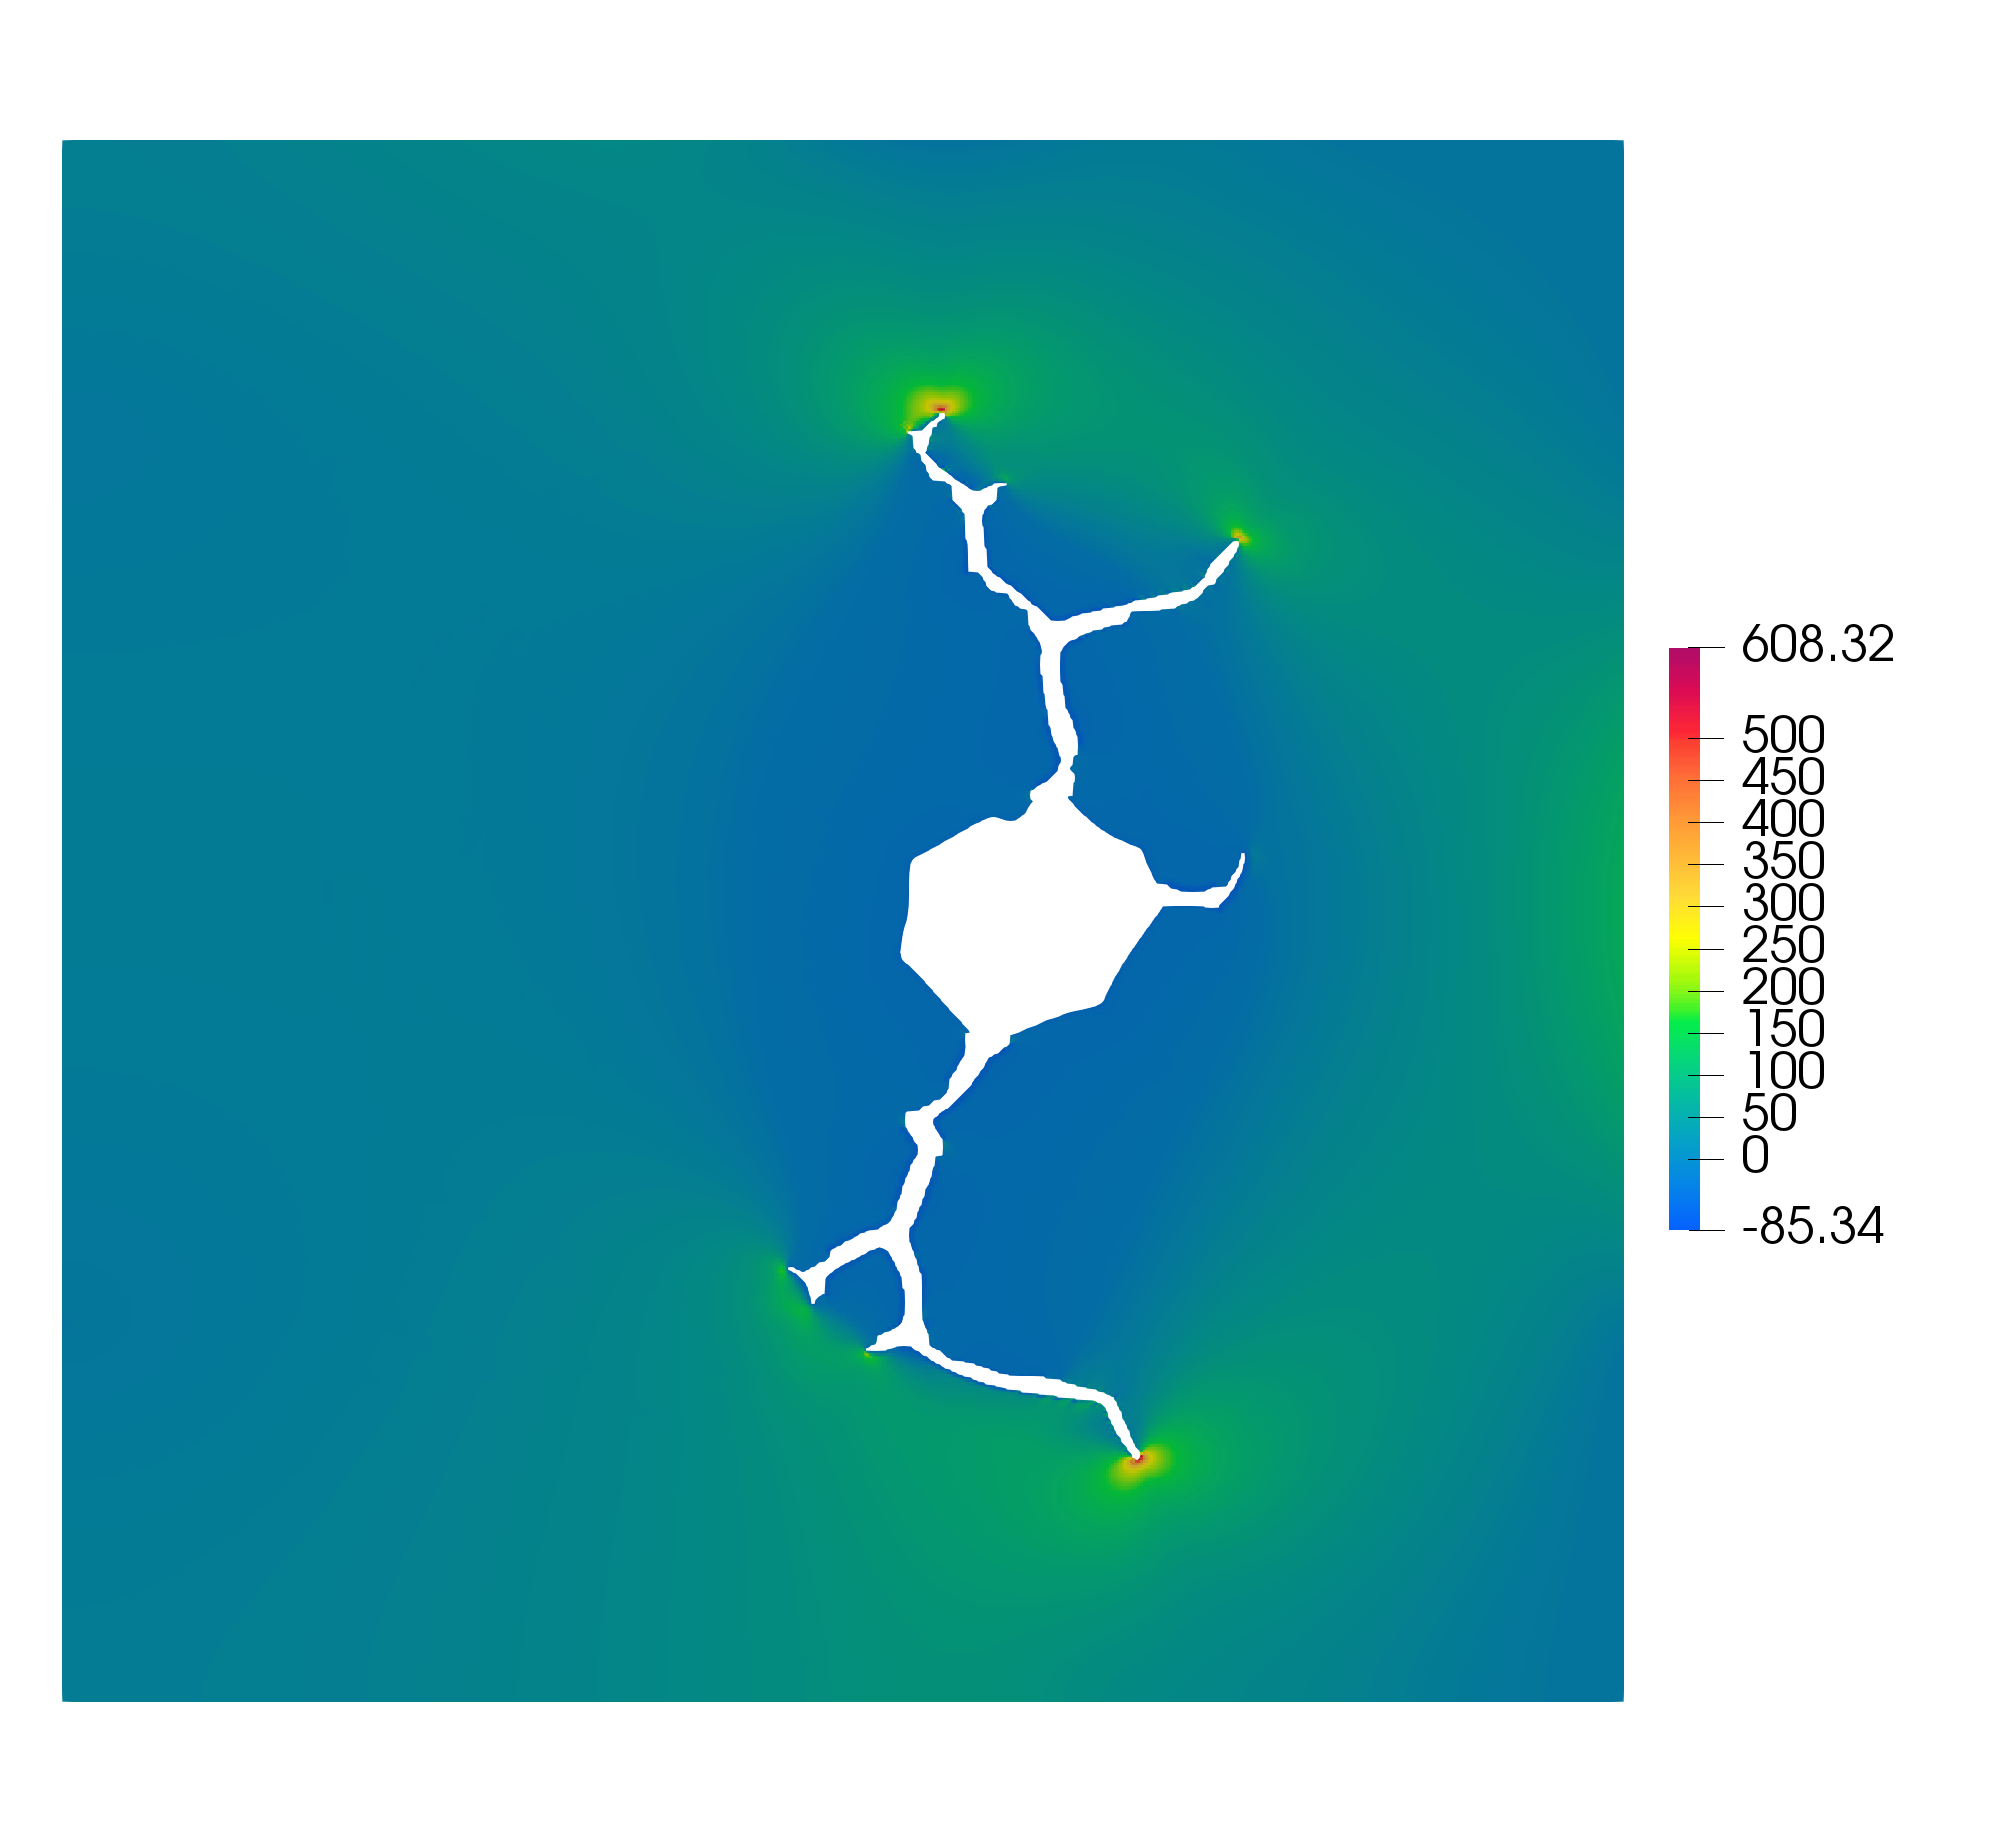
\includegraphics[width=\linewidth]{Chapter3/figures/partial_hbs_3_stress}
    \caption{}
  \end{subfigure}
  \caption[Crack propagation at different recrystallization stages.]{ (a, c, e) Crack paths superimposed on the microstructure and (b, d, f) contour plots of the maximum principal stress assuming different recrystallization stages: (a-b) $25\%$ recrystallization, (c-d) $60\%$ recrystallization, (e-f) $100\%$ recrystallization. }
  \label{fig:partial_hbs}
\end{figure}


\chapter{Cohesive Fracture: Soil Dessication}
\label{section: Chapter4}

\section{Introduction}
\label{section: Chapter4/intro}

In this chapter, a phase-field for cohesive fracture model is used to simulate pervasive cracking in thin films. A new strain energy split is proposed to enforce frictionless contact conditions in the vicinity of diffuse fracture surfaces. In contrast to existing splits that have been proposed, our approach completely prevents tractions from being transmitted across fully damaged surfaces that are loaded in tension. Spatial variations of material properties are incorporated into our model, and we demonstrate, through forward analysis and by solving an inverse problem, how crack network morphology can be influenced by stochastic spatially-varying material properties.

To prevent crack growth under compression, phase-field models of fracture typically employ some form of tension-compression asymmetric split in the strain energy. Two popular approaches are the spectral decomposition \cite{miehe_2010_p1, miehe_2010_p2} and the volumetric-deviatoric decomposition \cite{AMOR20091209}. Both the spectral decomposition and the volumetric-deviatoric decomposition are variational and can be fit within the current variational framework.
Although these variational approaches represent crack growth reasonably well for a broad range of problems, they do not completely preclude the transmission of tractions across fully damaged surfaces.   In part, this is by design.  The decompositions are designed to allow compressive tractions to be transmitted across fully damaged surfaces.  But since they are developed from the full stress or strain as opposed to the surface tractions, they can also allow umwanted tensile or shear tractions to be transmitted. This can give rise to spurious macro-scale responses in some situations.
\citet{strobl2015novel} proposed constitutive relations that satisfy the boundary conditions on diffuse crack surfaces by taking into account the crack orientation. Although the use of such a constitutive model violated the fundamental variational structure of phase-field models, it was shown to yield better results in some fracture problems \cite{strobl2016constitutive}.  A similar approach was presented by  \citet{fei2019phase, fei2020phasefield} to extend the model to better account for frictional contact conditions at crack surfaces.  Finally, we mention the recent work of \citet{Landis-fatigue}, in which the standard spectral split was modified to better guard against crack growth in compression.

In this chapter, we propose a variational strain energy split that enforces frictionless contact conditions.  Importantly, the split effectively prevents the transmission of tractions across fully-damaged surfaces that are loaded in tension.
The proposed split leads to a decomposition that is shown to be important in mode II and mixed-mode fracture problems.
The new phase-field model is then applied to study the classical problem of the fracture of thin films bonded to thick substrates.  Due to the accumulation of inelastic strain and the stiffness mismatch between the film and the substrate, cracks form either transversely through the thickness of the film, referred to as ``channeling'', or at the interface, referred to as ``debonding''.  Film-substrate systems exist across a wide span of application problems, from technological systems such as nuclear fuel pellet--cladding interactions (PCI) \cite{roberts1977pellet, michel20083d, jernkvist1995model, nagase2004effect, billone2008cladding}
to more common civil infrastructure examples such as pavement asphalts \cite{el2005calibration, el2009methodology, saar2010automatic, button2007guidelines, yildirim2006field}.
The study of fracture in these systems is driven by an interest in both understanding the underlying mechanisms and in preventing crack nucleation and evolution.  In the current work, we confine attention to transverse channeling cracks in the film.  When a system of cracks nucleate, branch and coalesce, complicated crack networks appear in the thin films. Hutchinson and Suo~\cite{hutchinson1991mixed} provides a
comprehensive review of crack patterns in film-substrate systems.

The fracture of thin films bonded to substrates has been studied using model-based simulations based on a wide range of methodologies.  These problems are challenging to simulate because they involve pervasive crack nucleation, branching, and coalescence.   Phenomenological spring models were developed and employed by \citet{crosby1997fragmentation, leung2000pattern} and \citet{ sadhukhan2011crack}. \citet{zhang2017modeling} applied a cohesive zone method to study the film-substrate interface debonding, and \citet{sanchez2014modeling}
proposed a mesh fragmentation technique to simulate three-dimensional crack morphologies. Although such techniques are known to produce mesh-dependent results, the resulting crack networks were found to be satisfactory. \citet{liang2003evolving, sukumar2003modeling} and \citet{huang2003modeling} modeled thin film cracking using the eXtended Finite Element Method (XFEM) which allowed for the cracks to evolve independently of the finite-element mesh.

The aforementioned analytical and numerical efforts have provided a great deal of insight into the factors controlling the fracture of thin films.  In particular, the mechanical properties that govern the spacing between cracks have been studied by \citet{hutchinson1991mixed, xia2000crack} and most recently by \citet{yin2008explicit}. In contrast,  the connection between spatial variations in material properties and the morphology of the resulting crack patterns has received fairly little attention. This is despite experimental evidence that crack morphologies are sensitive to spatial variations in material properties, see, e.g. \citet{kitsunezaki2016shaking, kitsunezaki2017stress, halasz2017effect, kitsunezaki2017memory} and \citet{nakahara2018mechanism}. To our knowledge, while some previous model-based simulations of thin-film fracture have incorporated random material properties, they have not specifically considered spatial fluctuations and the construction of proper stochastic models. More broadly, the literature on probabilistic modeling for fracture simulations remains scarce. In \cite{Acton2018}, variability in fracture strength was estimated from multiscale simulations, and spatially-varying mesoscale properties were subsequently integrated into an asynchronous spacetime discontinuous Galerkin finite element based fracture model to study the impact on fragmentation. The integration of apparent elasticity coefficients in a multiscale-informed phase-field formulation was investigated in \cite{Hun2019}, with the aim of reproducing variability in the macroscopic response. The fracture toughness was modeled as deterministic and homogeneous, and was identified by solving an inverse problem. In \cite{Peco2019}, a continuum mapping of the meso-scale structure to the packing fraction at the macro-scale was employed to introduce a random component to phase-field simulations of surfactant-induced fracture of particle rafts. In this chapter, we construct a probabilistic model for the critical fracture energy and the fracture toughness, modeled as (potentially correlated) random fields, and examine their influence on the random morphology of the resulting fracture patterns.

Our model-based simulations of thin-film fracture for systems with spatially-variable material properties are facilitated in this work through the adoption of an extension of phase-field models to cohesive fracture \cite{wu2016thermodynamically, wu2017unified, geelen2019phase}. Phase-field for cohesive fracture models incorporate the original proposition by \citet{xia2000crack} regarding a ``critical fracture energy''. The regularization length is decoupled from the material properties in these approaches, and the critical strength and the fracture toughness of the material are no longer strongly correlated. This independence permits simulations of drying in systems with realistic material properties for typical clays or soils, for example, without compromising the magnitude of the critical strength or requiring  regularization lengths that are larger than the specimen dimensions.  It also allows systems with spatially-variable fracture properties to be studied using a spatially-constant regularization length,  greatly improving the fidelity of the numerical calculations.

This chapter is organized as follows. \Cref{section: Chapter4/theory} the constitutive choices and stochastic models for fracture properties.  In \Cref{section: Chapter4/verification}, several numerical examples of benchmark problems in quasi-static fracture mechanics are provided to illustrate the efficacy of the new approach to enforcing frictionless contact conditions.  The main results of this work are provided in \Cref{section: Chapter4/examples}, where the new model is used to study the formation of crack networks in thin films and in soil desiccation problems.  In particular, model-based simulations are used to examine how the fragment statistics and fracture morphologies are influenced by spatial variations in the fracture properties.  Comparisons with both theory and experimental observations are provided.


\section{Theory}
\label{section: Chapter4/theory}

%%%%%%%%%%%%%%%%%%%%%%%%%%%%%%%%%%%%%%%%%%%%%%%%%%%%%%%%%%%%%%%%%%%%%%%%%%%%%%%%%%%%%%%%%%%
%%%%%%%%%%%%%%%%%%%%%%%%%%%%%%%%%%%%%%%%%%%%%%%%%%%%%%%%%%%%%%%%%%%%%%%%%%%%%%%%%%%%%%%%%%%
%%%%%%%%%%%%%%%%%%%%%%%%%%%%%%%%%%%%%%%%%%%%%%%%%%%%%%%%%%%%%%%%%%%%%%%%%%%%%%%%%%%%%%%%%%%
%%%%%%%%%%%%%%%%%%%%%%%%%%%%%%%%%%%%%%%%%%%%%%%%%%%%%%%%%%%%%%%%%%%%%%%%%%%%%%%%%%%%%%%%%%%
%%%%%%%%%%%%%%%%%%%%%%%%%%%%%%%%%%%%%%%%%%%%%%%%%%%%%%%%%%%%%%%%%%%%%%%%%%%%%%%%%%%%%%%%%%%
%%%%%%%%%%%%%%%%%%%%%%%%%%%%%%%%%%%%%%%%%%%%%%%%%%%%%%%%%%%%%%%%%%%%%%%%%%%%%%%%%%%%%%%%%%%
%%%%%%%%%%%%%%%%%%%%%%%%%%%%%%%%%%%%%%%%%%%%%%%%%%%%%%%%%%%%%%%%%%%%%%%%%%%%%%%%%%%%%%%%%%%
%%%%%%%%%%%%%%%%%%%%%%%%%%%%%%%%%%%%%%%%%%%%%%%%%%%%%%%%%%%%%%%%%%%%%%%%%%%%%%%%%%%%%%%%%%%
%%%%%%%%%%%%%%%%%%%%%%%%%%%%%%%%%%%%%%%%%%%%%%%%%%%%%%%%%%%%%%%%%%%%%%%%%%%%%%%%%%%%%%%%%%%
%%%%%%%%%%%%%%%%%%%%%%%%%%%%%%%%%%%%%%%%%%%%%%%%%%%%%%%%%%%%%%%%%%%%%%%%%%%%%%%%%%%%%%%%%%%
\subsection{Constitutive choices}

Similar constitutive choices made in \Cref{section: Chapter3} used to model cohesive fracture. In this chapter, the material is assumed to be isotropic while not necessarily homogeneous. Quasi-static and isothermal conditions are assumed to hold. No viscous regularization is incorporated, i.e. the dual kinetic potentials are zero. Following the variational framework (\Cref{section: Chapter2}), the Helmholtz free energy density is decomposed as
\begin{align}
  \psi = \psi^e + \psi^f + \psi^i,
\end{align}
where $\psi^e$ is the strain-energy density and $\psi^f$ is the fracture energy density. In the two dimensional simplification of the film-substrate system, $\psi^i$ represents the interfacial energy density that arises from the stiffness mismatch between the film and the substrate at the interface.

The same definition of the strain-energy density as in \eqref{eq: chapter 3 strain-energy density} and consequently the same stress-strain relation \eqref{eq: chapter 3 stress strain relation} are used. The following crack geometric function and degradation function are used to model cohesive fracture:
\begin{align}
  \alpha = d, \quad g = \dfrac{(1-d)^2}{(1-d)^2+md(1+pd)}, \quad m = \dfrac{3 \Gc}{8 l \psi_c}.
\end{align}
This degradation function is hereinafter referred to as the Lorentz (or in general the Lorentz-type) degradation function\footnote{Later on, the Lorentz-type degradation function may be denoted as $g^\text{Lorentz}$ to distinguish from the quadratic degradation function $g^\text{Quadratic} = (1-d)^2$.}.

\begin{remark}
  With a view towards the following stochastic analysis of fracture properties, the use of a Lorentz-type degradation function is necessary. According to one-dimensional analyses in \cite{geelen2019phase,wu2017unified}, the use of Lorentz-type degradation functions decouples the phase-field regularization length from the critical fracture energy, in the sense that the critical fracture energy $\psi^c$ may now be treated as a separate material property and later on as a \emph{marginally independent} random field, and the phase-field regularization length can truly be a numerical regularization parameter which the $\Gamma$-convergence properties of the model depend upon.
\end{remark}

The interfacial energy density describes the stiffness mismatch between the film and the substrate at the interface. The interfacial energy density and its thermodynamic conjugates are defined as
\begin{subequations}
  \begin{align}
    \psi^i                & = \dfrac{1}{2}g\dfrac{G}{hH}\bs{\upphi}\cdot\bs{\upphi},      \\
    \psi^i_{,\bs{\upphi}} & = g\dfrac{G}{hH}\bs{\upphi},                                  \\
    \psi^i_{,d}           & = \dfrac{1}{2}g_{,d}\dfrac{G}{hH}\bs{\upphi}\cdot\bs{\upphi}. 
  \end{align}
\end{subequations}

The gonverning equations can be summarized as
\begin{align}
  \divergence \stress - g\dfrac{G}{hH}\bs{\upphi} & = \bs{0}, \label{eq: chapter 4 momentum balance} \\
  \divergence \bs{\xi} - f                        & = 0,                                             
\end{align}
supplemented by the constitutive relations \eqref{eq: chapter 3 stress strain relation} and
\begin{align}
  \bs{\xi} = \dfrac{3\Gc l}{4} \grad d + \psi^e_{,\grad d}, \quad f = \dfrac{3\Gc}{8l}\alpha_{,d} + \psi^e_{,d} + \dfrac{1}{2}g_{,d}\dfrac{G}{hH}\bs{\upphi}\cdot\bs{\upphi}.
\end{align}
Note that \eqref{eq: chapter 4 momentum balance} ressembles a shear-lag model, and the additional term in $\bs{\xi}$ comes from the contact split to be introduced in \Cref{section: Chapter4/theory/contact_split}.

%%%%%%%%%%%%%%%%%%%%%%%%%%%%%%%%%%%%%%%%%%%%%%%%%%%%%%%%%%%%%%%%%%%%%%%%%%%%%%%%%%%%%%%%%%%
%%%%%%%%%%%%%%%%%%%%%%%%%%%%%%%%%%%%%%%%%%%%%%%%%%%%%%%%%%%%%%%%%%%%%%%%%%%%%%%%%%%%%%%%%%%
%%%%%%%%%%%%%%%%%%%%%%%%%%%%%%%%%%%%%%%%%%%%%%%%%%%%%%%%%%%%%%%%%%%%%%%%%%%%%%%%%%%%%%%%%%%
%%%%%%%%%%%%%%%%%%%%%%%%%%%%%%%%%%%%%%%%%%%%%%%%%%%%%%%%%%%%%%%%%%%%%%%%%%%%%%%%%%%%%%%%%%%
%%%%%%%%%%%%%%%%%%%%%%%%%%%%%%%%%%%%%%%%%%%%%%%%%%%%%%%%%%%%%%%%%%%%%%%%%%%%%%%%%%%%%%%%%%%
%%%%%%%%%%%%%%%%%%%%%%%%%%%%%%%%%%%%%%%%%%%%%%%%%%%%%%%%%%%%%%%%%%%%%%%%%%%%%%%%%%%%%%%%%%%
%%%%%%%%%%%%%%%%%%%%%%%%%%%%%%%%%%%%%%%%%%%%%%%%%%%%%%%%%%%%%%%%%%%%%%%%%%%%%%%%%%%%%%%%%%%
%%%%%%%%%%%%%%%%%%%%%%%%%%%%%%%%%%%%%%%%%%%%%%%%%%%%%%%%%%%%%%%%%%%%%%%%%%%%%%%%%%%%%%%%%%%
%%%%%%%%%%%%%%%%%%%%%%%%%%%%%%%%%%%%%%%%%%%%%%%%%%%%%%%%%%%%%%%%%%%%%%%%%%%%%%%%%%%%%%%%%%%
%%%%%%%%%%%%%%%%%%%%%%%%%%%%%%%%%%%%%%%%%%%%%%%%%%%%%%%%%%%%%%%%%%%%%%%%%%%%%%%%%%%%%%%%%%%
\subsection{Enforcing the traction-free boundary condition}
\label{section: Chapter4/theory/contact_split}

Widely used active/inactive splits are spectral split \cite{miehe_2010_p1, miehe_2010_p2} and volumetric-deviatoric split \cite{amor_2009}.  Unfortunately, neither the spectral split nor the volumetric-deviatoric split completely prevent tensile or shear tractions from being transmitted across fully-damaged surfaces.  Accordingly, we now develop a split that is motivated by the consideration of frictionless contact conditions along fully damaged surfaces.

We begin by recalling the standard Kuhn-Tucker optimality conditions for frictionless contact under small deformation, which can be written as
\begin{equation}
  t_N \geqslant 0, \quad u_I \leqslant 0, \quad t_N u_I = 0,
\end{equation}
where $t_N$ is the contact pressure and $u_I$ denotes the interpenetration between the contact surfaces.  The contact pressure is typically obtained from the stress and the exterior normal of the contact surface.  In regularized models of fracture, however, it can be difficult to identify a unique surface based on the phase field.  Accordingly, we rely on the gradient of the phase field to construct an approximate normal $\xnormal$, viz.
\begin{equation}
  \xnormal = \frac{\grad d}{ \norm{\grad d} },
\end{equation}
and calculate the normal pressure as
\begin{equation}
  \label{eq: pressure}
  t_N = -\xnormal\cdot\stress\xnormal.
\end{equation}
Our split keys off the sign of the normal pressure, by isolating the cases of a positive pressure (for contact) from a negative pressure (for opening).  In particular, we construct a ``normal-tangential'' stress decomposition of the form
\begin{equation}
  \stress  = \stress_n^{+} + \stress_n^{-}  + \stress_t ,
\end{equation}
where
\begin{equation}
  \stress_n^\pm = \macaulay{-t_N}_\pm\xnormal\otimes\xnormal, \quad  \stress_t = \stress - \stress_n^+ - \stress_n^-,
\end{equation}

In the vicinity of the regularized crack surface, we then propose the use of a stress-based strain-energy split, hereafter referred to as the \textit{contact split},
that takes the form:
\begin{subequations}
  \begin{align}
     & \psi^e = g\psi^e_\activepart + \psi^e_\inactivepart , \label{eq: odd begin}                                                            \\
     & \psi^e_\activepart = \dfrac{1}{2}\stress_\activepart:\strain, \quad \psi^e_\inactivepart = \dfrac{1}{2}\stress_\inactivepart:\strain , \\
     & \stress_\activepart = \stress_n^+ + \stress_t, \quad \stress_\inactivepart = \stress_n^-.                                              
  \end{align}
\end{subequations}
After a lengthy but straight-forward derivation, the corresponding constitutive relation follows as:
\begin{align}
  \stress  = g(d)\stress_\activepart + \stress_\inactivepart , \label{eq: odd end}
\end{align}
and
\begin{subequations}
  \begin{align}
    {\psi^e_\activepart}_{,\grad d}   & = \dfrac{1}{\norm{\grad d}} \left[ 2 \macaulay{-t_N}_- \varepsilon_N \xnormal - H(t_N) \varepsilon_N \stress\xnormal - \macaulay{-t_N}_- \strain\xnormal \right], \\
    {\psi^e_\inactivepart}_{,\grad d} & = -{\psi^e_\inactivepart}_{,\grad d},                                                                                                                             
  \end{align}
\end{subequations}
with $\varepsilon_N = \xnormal\cdot\strain\xnormal$.

It bears emphasis that the proposed strain-energy split only serves to enforce the crack surface traction free boundary condition, and it is not reasonable to expect it to reliably govern crack nucleation and growth. In this chapter, to ensure that the contact split is applied only in the vicinity of the crack surface, we impose a simple threshold $d_c$ such that we apply
\begin{align*}
  \begin{cases}
    \text{the contact split \eqref{eq: odd begin} to \eqref{eq: odd end}, } d \geqslant d_c \\
    \text{the strain-based spectral split \cite{miehe_2010_p1, miehe_2010_p2}, } d < d_c.
  \end{cases}
\end{align*}

\begin{remark}
  Alternative to a threshold, in principle a total energy could be constructed using a blending function that transitions between a standard split and the contact split.
\end{remark}

It can be shown that the definition of the contact pressure \eqref{eq: pressure} follows by relaxing the frictionless constraint into a minimization problem, and $t_N$ is therefore the best scalar quantity one can choose to approximate the traction-free boundary condition:
\begin{subequations}
  \begin{align}
    \min\limits_{t_N} \quad & \ \norm{\stress_t(t_N)\xnormal}^2                                                                                    \\
    =                       & \ \norm{(\stress-\macaulay{-t_N}_+\xnormal\otimes\xnormal-\macaulay{-t_N}_- \xnormal\otimes\xnormal)\cdot\xnormal}^2 \\
    =                       & \ \norm{(\stress+t_N \xnormal\otimes\xnormal)\cdot\xnormal}^2                                                        \\
    =                       & \ t_N^2 + 2t_N\xnormal\cdot\stress\xnormal + \norm{\stress\xnormal}^2,                                               
  \end{align}
\end{subequations}
and the minimizer is
\begin{align}
  t_N = \argmin\limits_{t_N} \left( t_N^2 + 2t_N\xnormal\cdot\stress\xnormal + \norm{\stress\xnormal}^2 \right) = -\xnormal\cdot\stress\xnormal .
\end{align}

%%%%%%%%%%%%%%%%%%%%%%%%%%%%%%%%%%%%%%%%%%%%%%%%%%%%%%%%%%%%%%%%%%%%%%%%%%%%%%%%%%%%%%%%%%%
%%%%%%%%%%%%%%%%%%%%%%%%%%%%%%%%%%%%%%%%%%%%%%%%%%%%%%%%%%%%%%%%%%%%%%%%%%%%%%%%%%%%%%%%%%%
%%%%%%%%%%%%%%%%%%%%%%%%%%%%%%%%%%%%%%%%%%%%%%%%%%%%%%%%%%%%%%%%%%%%%%%%%%%%%%%%%%%%%%%%%%%
%%%%%%%%%%%%%%%%%%%%%%%%%%%%%%%%%%%%%%%%%%%%%%%%%%%%%%%%%%%%%%%%%%%%%%%%%%%%%%%%%%%%%%%%%%%
%%%%%%%%%%%%%%%%%%%%%%%%%%%%%%%%%%%%%%%%%%%%%%%%%%%%%%%%%%%%%%%%%%%%%%%%%%%%%%%%%%%%%%%%%%%
%%%%%%%%%%%%%%%%%%%%%%%%%%%%%%%%%%%%%%%%%%%%%%%%%%%%%%%%%%%%%%%%%%%%%%%%%%%%%%%%%%%%%%%%%%%
%%%%%%%%%%%%%%%%%%%%%%%%%%%%%%%%%%%%%%%%%%%%%%%%%%%%%%%%%%%%%%%%%%%%%%%%%%%%%%%%%%%%%%%%%%%
%%%%%%%%%%%%%%%%%%%%%%%%%%%%%%%%%%%%%%%%%%%%%%%%%%%%%%%%%%%%%%%%%%%%%%%%%%%%%%%%%%%%%%%%%%%
%%%%%%%%%%%%%%%%%%%%%%%%%%%%%%%%%%%%%%%%%%%%%%%%%%%%%%%%%%%%%%%%%%%%%%%%%%%%%%%%%%%%%%%%%%%
%%%%%%%%%%%%%%%%%%%%%%%%%%%%%%%%%%%%%%%%%%%%%%%%%%%%%%%%%%%%%%%%%%%%%%%%%%%%%%%%%%%%%%%%%%%
\subsection{Stochastic models for fracture properties}
\label{section: Chapter4/theory/stochastic}

In this chapter, we allow for material property inhomogeneity in the macroscopic continuum model. Specifically, we introduce the random field $\{\bs{P}(btX) = (P_1(btX), P_2(btX)), btX \in \body\}$ defined on the probability space $(\Theta, \Sigma, P)$, indexed by $\body$ and with values in $\field{R}_{>0} \times \field{R}_{>0}$, such that $\{P_1(btX), btX \in \body\}$
(respectively $\{P_2(btX), btX \in \body\}$) is a prior representation of $\{\Gc(btX), btX \in \body\}$ (respectively $\{\psi_c(btX), btX \in \body\}$).
Due to the restrictions on the state space, the bivariate random field $\{\bs{P}(btX), btX \in \body\}$ is non-Gaussian. In order to model nongaussianity, the random field $\{\bs{P}(btX), btX \in \body\}$ is \textit{defined} as
\begin{align}
  \bs{P}(btX) := \fspace{T}(\bs{\Xi}(btX), btX)~, \quad \forall btX \in \body~, \label{eq: def-translation}
\end{align}
where $\fspace{T}$ is a measurable, nonlinear mapping and $\{\bs{\Xi}(btX),btX \in \body\}$ is a centered Gaussian random field with values in $\field{R}^2$ to be defined momentarily. From a methodological standpoint, it should be noticed that the transformation $\fspace{T}$ is constructed \textit{a priori} and used to define $\{\bs{P}(btX), btX \in \body\}$ such that the latter constitutes a surrogate capturing some essential features of $\{(\Gc(btX),\psi_c(btX)), btX \in \body\}$
(while exhibiting a low dimensional parameterization). In general, the existence of a nonlinear mapping $\fspace{T}$ such that \eqref{eq: def-translation} holds for a \textit{given} non-Gaussian field is not guaranteed; see, e.g., \cite{Grigoriu2009}.

%%%%%%%%%%%%%%%%%%%%%%%%%%%%%%%%%%%%%%%%%%%%%%%%%%%%%%%%%%%%%%%%%%%%%%%%%%%%%%%%%%%%%%%%%%%
%%%%%%%%%%%%%%%%%%%%%%%%%%%%%%%%%%%%%%%%%%%%%%%%%%%%%%%%%%%%%%%%%%%%%%%%%%%%%%%%%%%%%%%%%%%
%%%%%%%%%%%%%%%%%%%%%%%%%%%%%%%%%%%%%%%%%%%%%%%%%%%%%%%%%%%%%%%%%%%%%%%%%%%%%%%%%%%%%%%%%%%
%%%%%%%%%%%%%%%%%%%%%%%%%%%%%%%%%%%%%%%%%%%%%%%%%%%%%%%%%%%%%%%%%%%%%%%%%%%%%%%%%%%%%%%%%%%
%%%%%%%%%%%%%%%%%%%%%%%%%%%%%%%%%%%%%%%%%%%%%%%%%%%%%%%%%%%%%%%%%%%%%%%%%%%%%%%%%%%%%%%%%%%
%%%%%%%%%%%%%%%%%%%%%%%%%%%%%%%%%%%%%%%%%%%%%%%%%%%%%%%%%%%%%%%%%%%%%%%%%%%%%%%%%%%%%%%%%%%
%%%%%%%%%%%%%%%%%%%%%%%%%%%%%%%%%%%%%%%%%%%%%%%%%%%%%%%%%%%%%%%%%%%%%%%%%%%%%%%%%%%%%%%%%%%
%%%%%%%%%%%%%%%%%%%%%%%%%%%%%%%%%%%%%%%%%%%%%%%%%%%%%%%%%%%%%%%%%%%%%%%%%%%%%%%%%%%%%%%%%%%
%%%%%%%%%%%%%%%%%%%%%%%%%%%%%%%%%%%%%%%%%%%%%%%%%%%%%%%%%%%%%%%%%%%%%%%%%%%%%%%%%%%%%%%%%%%
%%%%%%%%%%%%%%%%%%%%%%%%%%%%%%%%%%%%%%%%%%%%%%%%%%%%%%%%%%%%%%%%%%%%%%%%%%%%%%%%%%%%%%%%%%%
\subsubsection{Construction of the Non-Gaussian Model}
\label{section: Chapter4/theory/stochastic/non_gaussian_model}

In this work, the transformation $\fspace{T}$ is constructed by imposing the family $\{f_{btX}\}_{btX\in\body}$ of first-order marginal distributions:
\begin{align}
  P_{\bs{P}(btX)}(d\bs{p}) = f_{btX}(\bs{p})\mathrm{d}\bs{p}~, \quad \forall btX \in \body~,
\end{align}
where $f_{btX}$ is the probability density function of $\bs{P}(btX)$, $btX$ being fixed in $\body$, and $\mathrm{d}\bs{p}=\mathrm{d}p_1\mathrm{d}p_2$ is the Lebesgue measure in $\field{R}^2$. It is assumed that $f_{btX}(\cdot) = f(\cdot; \bs{w}_{btX})$, where $\bs{w}_{btX}$ is a vector-valued hyperparameter indexed by $btX \in \body$. In order to simplify the analysis, we assume from now on that the aforementioned hyperparameter does not depend on location, and we write $f_{btX}(\cdot) = f(\cdot; \bs{w})$ using a slight abuse of notation.

The construction of $f$ can be achieved in many different ways. In what follows, the construction is performed by assuming that (i) $\Gc$ and $\psi_c$ (together with their inverses) are positive and have finite variance, for physical consistency, and (ii) the two fracture properties can exhibit some level of correlation. In accordance with information theory \cite{Jaynes1957a,Jaynes1957b} and more precisely, with the principle of maximum entropy \cite{Shannon1948a,Shannon1948b}, the first assumption leads to the consideration of Gamma marginal distributions. Following the notation introduced above, we shall impose that
\begin{align}
  P_{P_1(btX)}(dp_1) = f_\mathcal{G}(p_1; (\underline{p}_1,\delta_{1}))dp_1~, \quad \forall btX \in \body~,
\end{align}
and
\begin{align}
  P_{P_2(btX)}(dp_2) = f_\mathcal{G}(p_2; (\underline{p}_2,\delta_{2}))dp_2~, \quad \forall btX \in \body~,
\end{align}
where $f_\mathcal{G}(\cdot; (\underline{p}, \delta))$ denotes the univariate Gamma probability density function with mean $\underline{p}$ and coefficient of variation $\delta$. In this setting, the joint distribution of $\bs{P}(btX)$ must be constructed from the knowledge of the marginal laws associated with $P_1(btX)$ and $P_2(btX)$. This ill-posed problem does not admit a unique solution, and many possible forms were proposed in the case of a bivariate Gamma distribution (see, e.g., Chapter 8 in \cite{Balakrishnan2009} for a review). Here, we use the bivariate Gamma distribution derived by Moran using a copula \cite{Moran1969}:
\begin{align}
  f(\bs{p}) = \frac{1}{\sqrt{1-\rho^2}}\exp\left\{-\frac{1}{2(1-\rho^2)}\left[(\rho \tilde{p}_1)^2-2\rho \tilde{p}_1\tilde{p}_2+(\rho \tilde{p}_2)^2\right]\right\} f_\mathcal{G}(p_1; (\underline{p}_1,\delta_{1})) f_\mathcal{G}(p_2; (\underline{p}_2,\delta_{2})),
\end{align}
where $\rho \in (-1,1)$ is the (Pearson) correlation coefficient between $P_1(btX)$ and $P_2(btX)$ ($btX$ being fixed), and
\begin{align}
  \tilde{p}_i = \Phi^{-1}(F_\mathcal{G}(p_i; (\underline{p}_i,\delta_{i})))~, \quad i\in\{1,2\}~,
\end{align}
where $\Phi^{-1}$ is the inverse of the univariate Gaussian distribution function and $F_\mathcal{G}(\cdot; (\underline{p}_i,\delta_{i})))$ is the univariate Gamma distribution function with mean $\underline{p}_i$ and coefficient of variation $\delta_i$ (which is associated with $f_\mathcal{G}(\cdot; (\underline{p}_i, \delta_i))$), and that the extreme cases $\rho = \pm 1$ are also well defined; see \cite{Moran1969}. Notice that the vector of hyperparameters then reads as $\bs{w} = (\underline{p}_1,\delta_{1},\underline{p}_2,\delta_{2},\rho)$. It follows that
\begin{align}
  P_1(btX) = F_\mathcal{G}^{-1}(\Phi(\Upsilon_1(btX)); (\underline{p}_1,\delta_{1})))
\end{align}
and
\begin{align}
  P_2(btX) = F_\mathcal{G}^{-1}(\Phi(\Upsilon_2(btX)); (\underline{p}_2,\delta_{2})))
\end{align}
for any $btX$ fixed in $\body$, where $\bs{\Upsilon}(btX) = (\Upsilon_1(btX),\Upsilon_2(btX))$ is a centered Gaussian random variable with covariance matrix \cite{Moran1969}:
\begin{align}
  [C_{\bs{\Upsilon}}] =
  \begin{bmatrix}
    1    & \rho \\
    \rho & 1    
  \end{bmatrix}~.
\end{align}
Upon using the Cholesky factorization $[C_{\bs{\Upsilon}}] = [L_{\bs{\Upsilon}}]^\mathrm{T} [L_{\bs{\Upsilon}}]$, it can be deduced that $\{\bs{P}(btX), btX \in \body\}$ can be defined through
\begin{align}\label{eq: def-P1}
  P_1(btX) = F_\mathcal{G}^{-1}(\Phi(\Xi_1(btX)); (\underline{p}_1,\delta_{1})))~, \quad \forall btX \in \body~,
\end{align}
and
\begin{align}\label{eq: def-P2}
  P_2(btX) = F_\mathcal{G}^{-1}(\Phi(\rho \Xi_1(btX) + \sqrt{1-\rho^2} \Xi_2(btX)); (\underline{p}_2,\delta_{2})))~,\quad \forall btX \in \body~,
\end{align}
where $\{\bs{\Xi}(btX)=(\Xi_1(btX),\Xi_2(btX)), btX \in \field{R}^n\}$ is a centered Gaussian random field with statistically independent, centered Gaussian components such that $\bs{\Upsilon}(btX) = [L_{\bs{\Upsilon}}]^\mathrm{T}\bs{\Xi}(btX)$,
$\forall btX \in \body$. \Cref{eq: def-P1,eq: def-P2} define the nonlinear mapping $\fspace{T}$ introduced in \Cref{eq: def-translation} such that $\bs{P}(btX) = \fspace{T}(\bs{\Xi}(btX))$,
for all $btX \in \body$ (note that the spatial dependence of the transformation was dropped given the retained modeling assumptions). This relation can equivalently be stated as $\bs{P}(btX) = \fspace{T}^\ast(\bs{\Upsilon}(btX))$, with obvious notation. The Gaussian random fields are defined in the next section.

%%%%%%%%%%%%%%%%%%%%%%%%%%%%%%%%%%%%%%%%%%%%%%%%%%%%%%%%%%%%%%%%%%%%%%%%%%%%%%%%%%%%%%%%%%%
%%%%%%%%%%%%%%%%%%%%%%%%%%%%%%%%%%%%%%%%%%%%%%%%%%%%%%%%%%%%%%%%%%%%%%%%%%%%%%%%%%%%%%%%%%%
%%%%%%%%%%%%%%%%%%%%%%%%%%%%%%%%%%%%%%%%%%%%%%%%%%%%%%%%%%%%%%%%%%%%%%%%%%%%%%%%%%%%%%%%%%%
%%%%%%%%%%%%%%%%%%%%%%%%%%%%%%%%%%%%%%%%%%%%%%%%%%%%%%%%%%%%%%%%%%%%%%%%%%%%%%%%%%%%%%%%%%%
%%%%%%%%%%%%%%%%%%%%%%%%%%%%%%%%%%%%%%%%%%%%%%%%%%%%%%%%%%%%%%%%%%%%%%%%%%%%%%%%%%%%%%%%%%%
%%%%%%%%%%%%%%%%%%%%%%%%%%%%%%%%%%%%%%%%%%%%%%%%%%%%%%%%%%%%%%%%%%%%%%%%%%%%%%%%%%%%%%%%%%%
%%%%%%%%%%%%%%%%%%%%%%%%%%%%%%%%%%%%%%%%%%%%%%%%%%%%%%%%%%%%%%%%%%%%%%%%%%%%%%%%%%%%%%%%%%%
%%%%%%%%%%%%%%%%%%%%%%%%%%%%%%%%%%%%%%%%%%%%%%%%%%%%%%%%%%%%%%%%%%%%%%%%%%%%%%%%%%%%%%%%%%%
%%%%%%%%%%%%%%%%%%%%%%%%%%%%%%%%%%%%%%%%%%%%%%%%%%%%%%%%%%%%%%%%%%%%%%%%%%%%%%%%%%%%%%%%%%%
%%%%%%%%%%%%%%%%%%%%%%%%%%%%%%%%%%%%%%%%%%%%%%%%%%%%%%%%%%%%%%%%%%%%%%%%%%%%%%%%%%%%%%%%%%%
\subsubsection{Construction of the Underlying Gaussian Models}
\label{section: Chapter4/theory/stochastic/gaussian_model}

In accordance with the periodic assumption retained in the mechanical modeling framework, it is assumed that each random field $\{\Xi_i(btX), btX \in \field{R}^n\}$, $i \in \{1,2\}$, satisfies the invariance property $\Xi_i(btX) = \Xi_i(btX+pbtX')$ for all $btX \in \body$ and $btX' \in \field{Z}^n$
$P$-almost surely, where it is assumed (without loss of generality) that $\body = ([0,p])^n$. Consequently, the centered random field $\{\bs{\Xi}(btX), btX \in \field{R}^n\}$ is uniquely defined by its restriction to $\body$.  Assuming the stationary of this restriction in $\body$, the underlying Gaussian field is defined through the matrix-valued covariance function $\bs{\tau} \mapsto [\cor_{\bs{\Xi}}(\bs{\tau})] = \field{E}\{\bs{\Xi}(btX+\bs{\tau}) \otimes \bs{\Xi}(btX)\}$
such that
\begin{align}
  [\cor_{\bs{\Xi}}(\bs{\tau})] = \left[\begin{array}{cc}\cor_1(\bs{\tau}) & 0 \\0 & \cor_2(\bs{\tau}) \end{array}\right]~, \quad \forall \bs{\tau} \in ([0,p])^n~,
\end{align}
where $\cor_1$ and $\cor_2$ are the $p$-periodic covariance functions defining (the restrictions of) $\{\Xi_1(btX), btX \in \field{R}^n\}$ and $\{\Xi_2(btX), btX \in \field{R}^n\}$ (to $\body$), respectively.
For the sake of illustration, we assume similar covariance functions for the two Gaussian components, setting $\cor_1 = \cor_2 = \cor$,
and we consider the case of a separable covariance function in $\field{R}^2$:
\begin{align}
  \cor(\bs{\tau}) = \cor_1(\tau_1) \times \cor_2(\tau_2)~. \label{eq: composite covariance function}
\end{align}
We further assume that $\cor_1$ and $\cor_2$ only differ in the choice of hyperparameters, so that the above equation can be written, using an abuse of notation, as
\begin{align}
  \cor(\bs{\tau}) = \cor(\tau_1;L_1) \times \cor(\tau_2;L_2)~,
\end{align}
where $L_1 > 0$ and $L_2 > 0$ are model parameters controlling the correlation ranges of the fields along the directions defined by the canonical basis in $\field{R}^2$. The univariate covariance function $\cor$ is assumed to take the generic form
\begin{align}
  \cor_\phi(\tau; L) & = \exp\left( -c \phi(\tau; L)\right )~, \quad \forall \tau \in [0,p]~, \label{eq: def-generic-cov} 
\end{align}
where $c$ is a positive constant (that depends on both $\phi$ and $L$) to be defined and $\phi$ is a $p$-periodic function taken as
\begin{align}
  \phi(\tau; L) = \dfrac{|\sin\left( \pi\tau/p \right)|}{L} \quad \text{(Periodic Exponential, PE),} \label{eq: def-exp}
\end{align}
or
\begin{align}
  \phi(\tau; L) = \dfrac{\sin\left( \pi\tau/p \right)^2}{L^2} \quad \text{(Periodic Squared-Exponential, PSE)}~. \label{eq: def-sexp}
\end{align}
The subscript in the notation $\cor_\phi$ underlines the choice of a particular periodic function. The two functions defined by \eqref{eq: def-exp} and \eqref{eq: def-sexp} are specifically chosen so as to investigate the impact of sample path regularity on fracture simulation outcomes. In particular, and while both functions yield random fields of fracture properties that are mean-square continuous, the periodic squared-exponential covariance function obtained by combining \eqref{eq: def-generic-cov} and \eqref{eq: def-sexp} leads to mean-square differentiable fields which exhibit ``smooth'' realizations. On the contrary, the periodic exponential function defined by considering \eqref{eq: def-exp} yields random fields that are not mean-square differentiable and thus have much rougher realizations.

In order to ensure meaningful comparison between the covariance models, the normalization constants are determined such that the spatial correlation length along the direction of one main direction is equal to $L$, that is:
\begin{align}
  \int_0^{p/2} |\cor_\phi(\tau; L)| \mathrm{d}\tau = L~.
\end{align}
For later use, we introduce the normalized correlation length $L^* = L/p$. For the squared exponential model, the constant $c^{}_\text{PSE}$ is hence required to satisfy the nonlinear equation
\begin{align}
  \dfrac{1}{2}p\exp\left( -\dfrac{c^{}_\text{PSE}}{2L^2} \right)I_0(\dfrac{c^{}_\text{PSE}}{2L^2}) = L~, \label{eq: pse normalization}
\end{align}
where $I_0$ is the 0th order modified Bessel's function, whereas the constant $c^{}_\text{PE}$ associated with the exponential covariance kernel must satisfy
\begin{align}
  \dfrac{1}{2}p\left[ I_0\left(\dfrac{c^{}_\text{PE}}{L}\right) - S_0\left(\dfrac{c^{}_\text{PE}}{L}\right) \right] = L~, \label{eq: se normalization}
\end{align}
where $S_0$ is the 0th order modified Struve's function.
In this work, these equations are solved numerically using a Newton-Raphson solver.

It should be noticed that the covariance function $\bs{\tau} \mapsto [\cor_{\bs{\Upsilon}}(\bs{\tau})]$ defining the restriction of the Gaussian random field $\{\bs{\Upsilon}(btX), btX \in \field{R}^n\}$ to $\body$ is given by
\begin{align}
  [\cor_{\bs{\Upsilon}}(\bs{\tau})] = \left[\begin{array}{cc}\cor_1(\bs{\tau}) & \rho \cor_1(\bs{\tau}) \\\rho \cor_1(\bs{\tau}) & \rho^2 \cor_1(\bs{\tau}) + (1-\rho^2) \cor_2(\bs{\tau}) \end{array}\right]~, \quad \forall \bs{\tau} \in ([0,p])^n~,
\end{align}
which shows the role played by the parameter $\rho$ on the covariance function of $\{P_2(btX), btX \in \body\}$ (after the action of $\fspace{T}^*$).

%%%%%%%%%%%%%%%%%%%%%%%%%%%%%%%%%%%%%%%%%%%%%%%%%%%%%%%%%%%%%%%%%%%%%%%%%%%%%%%%%%%%%%%%%%%
%%%%%%%%%%%%%%%%%%%%%%%%%%%%%%%%%%%%%%%%%%%%%%%%%%%%%%%%%%%%%%%%%%%%%%%%%%%%%%%%%%%%%%%%%%%
%%%%%%%%%%%%%%%%%%%%%%%%%%%%%%%%%%%%%%%%%%%%%%%%%%%%%%%%%%%%%%%%%%%%%%%%%%%%%%%%%%%%%%%%%%%
%%%%%%%%%%%%%%%%%%%%%%%%%%%%%%%%%%%%%%%%%%%%%%%%%%%%%%%%%%%%%%%%%%%%%%%%%%%%%%%%%%%%%%%%%%%
%%%%%%%%%%%%%%%%%%%%%%%%%%%%%%%%%%%%%%%%%%%%%%%%%%%%%%%%%%%%%%%%%%%%%%%%%%%%%%%%%%%%%%%%%%%
%%%%%%%%%%%%%%%%%%%%%%%%%%%%%%%%%%%%%%%%%%%%%%%%%%%%%%%%%%%%%%%%%%%%%%%%%%%%%%%%%%%%%%%%%%%
%%%%%%%%%%%%%%%%%%%%%%%%%%%%%%%%%%%%%%%%%%%%%%%%%%%%%%%%%%%%%%%%%%%%%%%%%%%%%%%%%%%%%%%%%%%
%%%%%%%%%%%%%%%%%%%%%%%%%%%%%%%%%%%%%%%%%%%%%%%%%%%%%%%%%%%%%%%%%%%%%%%%%%%%%%%%%%%%%%%%%%%
%%%%%%%%%%%%%%%%%%%%%%%%%%%%%%%%%%%%%%%%%%%%%%%%%%%%%%%%%%%%%%%%%%%%%%%%%%%%%%%%%%%%%%%%%%%
%%%%%%%%%%%%%%%%%%%%%%%%%%%%%%%%%%%%%%%%%%%%%%%%%%%%%%%%%%%%%%%%%%%%%%%%%%%%%%%%%%%%%%%%%%%
\subsubsection{Fundamental Properties of the Random Field of Fracture Properties}

Based on the construction proposed in Sections \ref{section: Chapter4/theory/stochastic/non_gaussian_model} and \ref{section: Chapter4/theory/stochastic/gaussian_model}, the non-Gaussian random field $\{\bs{P}(btX), btX \in \body\}$ modeling the fracture properties satisfies the following properties:
\begin{enumerate}
  \item $P_i(btX) > 0$ for all $btX \in \body$ and $i \in \{1,2\}$, almost surely.
  \item $\{\bs{P}(btX), btX \in \body\}$ is of second order, $\field{E}\{\|\bs{P}(btX)\|^2\} < + \infty$ $\forall btX \in \body$.
  \item The field satisfies $\bs{P}((0, x_2)) = \bs{P}((p, x_2))$ and $\bs{P}((x_1, 0)) = \bs{P}((x_1, p))$, almost surely.
  \item The mean function $btX \mapsto \underline{\bs{p}}(btX) = \field{E}\{\bs{P}(btX)\}$ is given by $\underline{\bs{p}}(btX) = \underline{\bs{p}} = (\underline{p}_1, \underline{p}_2)$ for all $btX \in \body$.
  \item The covariance matrix at any location $btX \in \body$ reads as
        \begin{align}
          \field{E}\{(\bs{P}(btX) - \underline{\bs{p}}) \otimes (\bs{P}(btX) - \underline{\bs{p}})\} = \left[\begin{array}{cc} \underline{p}_1^2 \delta_1^2 &  \underline{p}_1 \underline{p}_2 \delta_1  \delta_2 \rho  \\[1mm] \underline{p}_1 \underline{p}_2 \delta_1  \delta_2 \rho & \underline{p}_2^2 \delta_2^2 \end{array}\right]~.
        \end{align}
\end{enumerate}
It can also be deduced that the random field $\{\bs{P}(btX), btX \in \body\}$ is mean-square continuous for the PE and PSE correlation functions introduced in Section \ref{section: Chapter4/theory/stochastic/gaussian_model}. Finally, the field is mean-square differentiable for the PSE covariance function.

Recall that in the properties above, $\underline{p}_1$ and $\underline{p}_2$ correspond to the desired mean values for the fracture toughness $\Gc$ and energy threshold $\psi_c$, and $\delta_1$ and $\delta_2$ are the coefficients of variation that control the statistical dispersions of these parameters. The parameter $\rho$ measures the level of correlation between the fracture properties.

%%%%%%%%%%%%%%%%%%%%%%%%%%%%%%%%%%%%%%%%%%%%%%%%%%%%%%%%%%%%%%%%%%%%%%%%%%%%%%%%%%%%%%%%%%%
%%%%%%%%%%%%%%%%%%%%%%%%%%%%%%%%%%%%%%%%%%%%%%%%%%%%%%%%%%%%%%%%%%%%%%%%%%%%%%%%%%%%%%%%%%%
%%%%%%%%%%%%%%%%%%%%%%%%%%%%%%%%%%%%%%%%%%%%%%%%%%%%%%%%%%%%%%%%%%%%%%%%%%%%%%%%%%%%%%%%%%%
%%%%%%%%%%%%%%%%%%%%%%%%%%%%%%%%%%%%%%%%%%%%%%%%%%%%%%%%%%%%%%%%%%%%%%%%%%%%%%%%%%%%%%%%%%%
%%%%%%%%%%%%%%%%%%%%%%%%%%%%%%%%%%%%%%%%%%%%%%%%%%%%%%%%%%%%%%%%%%%%%%%%%%%%%%%%%%%%%%%%%%%
%%%%%%%%%%%%%%%%%%%%%%%%%%%%%%%%%%%%%%%%%%%%%%%%%%%%%%%%%%%%%%%%%%%%%%%%%%%%%%%%%%%%%%%%%%%
%%%%%%%%%%%%%%%%%%%%%%%%%%%%%%%%%%%%%%%%%%%%%%%%%%%%%%%%%%%%%%%%%%%%%%%%%%%%%%%%%%%%%%%%%%%
%%%%%%%%%%%%%%%%%%%%%%%%%%%%%%%%%%%%%%%%%%%%%%%%%%%%%%%%%%%%%%%%%%%%%%%%%%%%%%%%%%%%%%%%%%%
%%%%%%%%%%%%%%%%%%%%%%%%%%%%%%%%%%%%%%%%%%%%%%%%%%%%%%%%%%%%%%%%%%%%%%%%%%%%%%%%%%%%%%%%%%%
%%%%%%%%%%%%%%%%%%%%%%%%%%%%%%%%%%%%%%%%%%%%%%%%%%%%%%%%%%%%%%%%%%%%%%%%%%%%%%%%%%%%%%%%%%%
\subsubsection{Stochastic Simulation Aspects}

Simulating realizations of the random field of fracture properties requires (i) drawing realizations of the underlying Gaussian random fields defined in \Cref{section: Chapter4/theory/stochastic/gaussian_model}, and (ii) evaluating the nonlinear transformations defined by \eqref{eq: def-P1} and \eqref{eq: def-P2}. Routines to compute the latter mappings are readily available in many scientific computing environments. Regarding the generation of the Gaussian fields, we presently resort to truncated Karhunen-Lo\`eve expansions. Each (mean-square continuous) random field $\{\Xi_i(btX), btX \in \field{R}^n\}$, $i \in \{1,2\}$, is thus expanded as
\begin{align}
  \Xi_i(btX) = \sum\limits_{k=1}^{q_i} \sqrt{\lambda_k} \eta_k \varphi_k(btX)~,
\end{align}
where $\{\eta_k\}_{k \geqslant 1}$ is a set of independent normalized Gaussian random variables, and $\{\lambda_k\}_{k \geqslant 1}$ and $\{\varphi_k\}_{k \geqslant 1}$ are the nonnegative eigenvalues (ordered as a nonincreasing sequence) and the associated orthonormal eigenfunctions of the covariance function that satisfy the following integral equation (which is a Fredholm integral equation of the second kind):
\begin{align}
  \int\limits_\body \cor(btX,btX')\varphi_k(btX') \diff{\bfX}' = \lambda_k\varphi_k(btX)~, \quad \forall btX \in \body~, \label{eq: FIE2}
\end{align}
where $\cor$ is the covariance kernel introduced in Section \ref{section: Chapter4/theory/stochastic/gaussian_model} (note the abuse of notation, with $\bs{\tau} = btX - btX'$). For arbitrary covariance functions, this integral equation can be solved by using a standard Galerkin formulation \cite{GhanemSpanos,LMK2010}: given a finite set of basis functions $\{\phi_j\}_{j=1}^{N_\text{node}} \subset L_2(\body)$,
each eigenfunction is approximated as
\begin{align}
  \varphi_k(btX) \approx \sum_{j=1}^{N_{\text{node}}} \alpha_{j}^{(k)}\phi_j(btX)~. \label{eq: eigenfunction approximation}
\end{align}
Substituting this approximation in the integral equation and enforcing the residual to be orthogonal to $\mathspan(\{\phi_j\}_{j=1}^{N_\text{node}})$, we obtain
\begin{align}
  \sum_{j=1}^{N_{\text{node}}} \alpha_{j}^{(k)} \int\limits_\body \int\limits_\body \cor(btX,btX') \phi_j(btX')\phi_\ell(btX) \diff{\bfX}' \diff{\bfX} = \sum_{j=1}^{N_{\text{node}}} \alpha_{j}^{(k)} \int\limits_\body \lambda_k \phi_j(btX)\phi_\ell(btX) \diff{\bfX}~. \label{eq: gevp}
\end{align}
Considering the above equation for all eigenfunctions leads to the generalized eigenvalue problem $[K] [A] = [\Lambda] [M] [A]$, where $[A]_{j\ell} = \alpha_j^{(\ell)}$, $[\Lambda]_{j\ell} = \lambda_j \delta_{j_\ell}$ (with $\delta_{j_\ell}$ the Kronecker delta), and $[K]$ and $[M]$ are the matrices with entries
\begin{align}
  [K]_{j\ell} = \int\limits_\body \int\limits_\body \cor(btX,btX') \phi_j(btX')\phi_\ell(btX) \diff{\bfX}' \diff{\bfX}~, \quad [M]_{j\ell} = \int\limits_\body \phi_j(btX)\phi_\ell(btX) \diff{\bfX}~.
\end{align}
For each Gaussian field $\{\Xi_i(btX), btX \in \field{R}^n\}$, the truncation order $q_i \leqslant N_{\text{node}}$ can be determined by analyzing the convergence of the error function
\begin{align}
  \varepsilon_{\text{KL}}(q) = 1-\left( \sum\limits_{k=1}^q \lambda_k \middle/ \sum\limits_{k=1}^{N_\text{node}} \lambda_k \right)~, \label{eq: truncation}
\end{align}
and by selecting $q_i$ such that $\varepsilon_{\text{KL}}(q_i) \leqslant \varepsilon_0$ for some given tolerance $0 < \varepsilon_0 \ll 1$.


\section{Verification}
\label{section: cohesive/verification}

\subsection{Edge-notched specimen}

\subsection{Crack propagation under biaxial tension}

\subsection{Reconstruction of the marginal PDF}


\section{Numerical examples}
\label{section: cohesive/examples}

In this section, we study in detail the formation of crack networks in thin films and soil dessication.  We begin
in Section \ref{s: application/1D} with a deterministic benchmark problem under quasi-one-dimensional conditions.  The spacing between fractures is calculated as a function of the driving force with the cohesive fracture model and compared against a linear elasticity solution. Attention is then turned to an investigation of the stochastic aspects of fracture with a two-dimensional plane stress model in Section \ref{s: Chapter4/2D}, wherein the fracture toughness and critical fracture energy are modeled as random fields.  Finally, in Section \ref{s: Chapter4/3D} we present stochastic simulations of a soil dessication process in three dimensions.

%%%%%%%%%%%%%%%%%%%%%%%%%%%%%%%%%%%%%%%%%%%%%%%%%%%%%%%%%%%%%%%%%%%%%%%%%%%%%%%%%%%%%%%%%%%
%%%%%%%%%%%%%%%%%%%%%%%%%%%%%%%%%%%%%%%%%%%%%%%%%%%%%%%%%%%%%%%%%%%%%%%%%%%%%%%%%%%%%%%%%%%
%%%%%%%%%%%%%%%%%%%%%%%%%%%%%%%%%%%%%%%%%%%%%%%%%%%%%%%%%%%%%%%%%%%%%%%%%%%%%%%%%%%%%%%%%%%
%%%%%%%%%%%%%%%%%%%%%%%%%%%%%%%%%%%%%%%%%%%%%%%%%%%%%%%%%%%%%%%%%%%%%%%%%%%%%%%%%%%%%%%%%%%
%%%%%%%%%%%%%%%%%%%%%%%%%%%%%%%%%%%%%%%%%%%%%%%%%%%%%%%%%%%%%%%%%%%%%%%%%%%%%%%%%%%%%%%%%%%
%%%%%%%%%%%%%%%%%%%%%%%%%%%%%%%%%%%%%%%%%%%%%%%%%%%%%%%%%%%%%%%%%%%%%%%%%%%%%%%%%%%%%%%%%%%
%%%%%%%%%%%%%%%%%%%%%%%%%%%%%%%%%%%%%%%%%%%%%%%%%%%%%%%%%%%%%%%%%%%%%%%%%%%%%%%%%%%%%%%%%%%
%%%%%%%%%%%%%%%%%%%%%%%%%%%%%%%%%%%%%%%%%%%%%%%%%%%%%%%%%%%%%%%%%%%%%%%%%%%%%%%%%%%%%%%%%%%
%%%%%%%%%%%%%%%%%%%%%%%%%%%%%%%%%%%%%%%%%%%%%%%%%%%%%%%%%%%%%%%%%%%%%%%%%%%%%%%%%%%%%%%%%%%
%%%%%%%%%%%%%%%%%%%%%%%%%%%%%%%%%%%%%%%%%%%%%%%%%%%%%%%%%%%%%%%%%%%%%%%%%%%%%%%%%%%%%%%%%%%
\subsection{One-Dimensional Simplification: Side View}

We begin by deriving an analytical solution for the fracture of a thin film bonded to a thick substrate, as shown in \Cref{fig: Chapter4/1D/simplification}.  Assuming that the planar dimensions of the film are much larger than its thickness, we first simplify the problem into a two-dimensional (or quasi 1D) plane-strain problem. The film is assumed to have Young's modulus $E_1$, Poisson's ratio $\nu_1$, and thickness $h$. The substrate has Young's modulus $E_0$, Poisson's ratio $\nu_0$, and thickness $H$.  The fracture of the film is driven by the underlying substrate being stretched an amount $\varepsilon_x$.  The problem with these simplifications and assumptions has been studied by many researchers, and analytical solutions from elasticity theory have been derived in several different ways.  The derivation presented herein most closely follows that provided in \citet{yin2008explicit}.

\begin{figure}
  \centering
  \begin{subfigure}[b]{0.35\textwidth}
    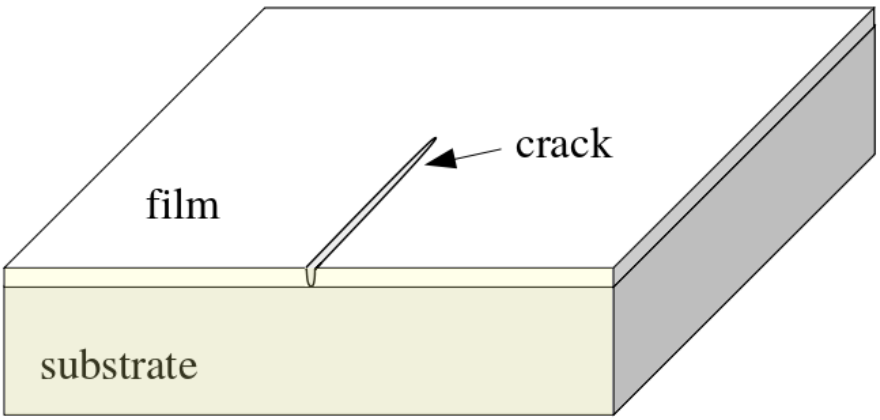
\includegraphics[width=\textwidth,scale=0.5]{Chapter4/figures/1D/side_view.png}
    \caption{}
  \end{subfigure}
  \begin{subfigure}[b]{0.45\textwidth}
    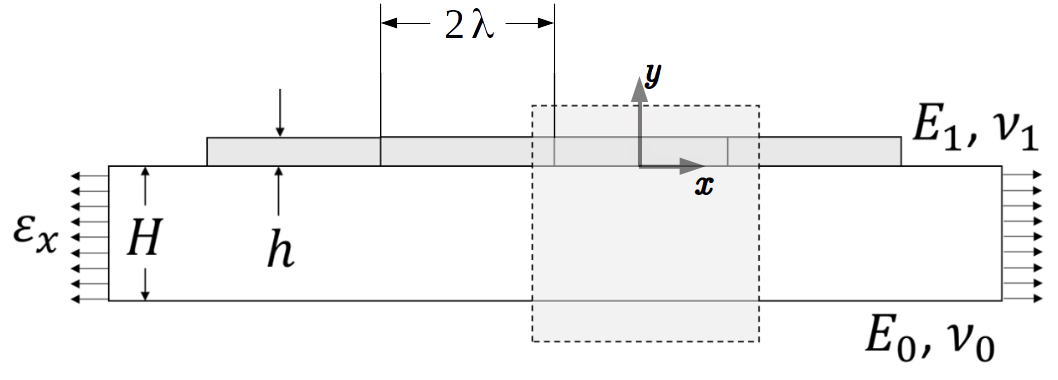
\includegraphics[width=\textwidth,scale=0.5]{Chapter4/figures/1D/1D_schematic.png}
    \caption{}
    \label{fig: Chapter4/1D/schematic}
  \end{subfigure}
  \caption{Description of a one-dimensional model for thin-film cracking.  (a) Side view  (highlighted in yellow) of the geometry (b) schematic representation of the side view. The elasticity solution is derived for the region highlighted with the shaded box, i.e.\ between the two discontinuities across the thin film. The coordinate system is centered at the middle of the bottom surface of the thin film. }
  \label{fig: Chapter4/1D/simplification}
\end{figure}


\begin{figure}
  \centering
  \begin{overpic}[scale=0.55]{Chapter4/figures/1D/supersuperposition.png}
    \put(12,-4){(a)}
    \put(46,-4){(b)}
    \put(80,-4){(c)}
  \end{overpic}
  \vspace{0.2in}
  \caption{ The principal of ``super-superposition'' applied to the region of interest marked in \Cref{fig: Chapter4/1D/schematic}. The analytical solution is derived based on the boundary conditions shown in (c). }
  \label{fig: Chapter4/1D/supersuperposition}
\end{figure}


With the increase of the tensile strain in the substrate, some uniformly distributed discontinuities with spacing $2\lambda$ form across the thickness of the film. We assume that no debonding occurs and that the vertical component of the displacement does not vary in the horizontal direction, i.e.
\begin{align}
  u_y(x,y) = u_y(y) .
\end{align}
The plane-strain equilibrium equation in the x--direction is written as
\begin{align}
  \dfrac{E_1}{1-\nu_1^2}u_{x,xx} + \mu_1u_{x,yy} = 0 ,
\end{align}
where $\mu_1$ denotes the shear modulus of the film.  This is supplemented by appropriate boundary conditions (\Cref{fig: Chapter4/1D/supersuperposition})
\begin{align}
  u_x(0,y)                                                    & = 0 ,                                    \\
  u_{x,y}(x,h)                                                & = 0 ,                                    \\
  \dfrac{1}{h}\int\limits_{0}^h \sigma_x(\lambda,y)\text{ d}y & = -\dfrac{E_1}{1-\nu_1^2}\varepsilon_x .
\end{align}
We obtain the closed-form solution to the displacement field
\begin{align}
  u_x(x,y) = \varepsilon_xx-\dfrac{\sinh(cx/h)}{\cosh(c\lambda/h)}\dfrac{\cos(d(1-y/h))}{\sin(d)}\sqrt{\dfrac{E_1}{\mu_1(1-\nu_1^2)}}h\varepsilon_x ,
\end{align}
where $c$ and $d$ are functions of Dundur's parameters $\alpha$ and $\beta$. Following \cite{BEUTH19921657,xia2000crack,yin2008explicit}, $c$ and $d$ can be computed as:
\begin{align}
   & c = \dfrac{2}{\pi k(\alpha,\beta)}, \quad d = \sqrt{\dfrac{2}{1-\nu_1}}c ,                                                                          \\
   & \alpha = \dfrac{\Bar{E}_1-\Bar{E}_0}{\Bar{E}_1+\Bar{E}_0}, \quad \beta = \dfrac{\mu_1(1-2\nu_0)-\mu_0(1-2\nu_1)}{2\mu_1(1-\nu_0)+2\mu_0(1-\nu_1)} , \\
   & k(\alpha,\beta) \approx k(\alpha) = \dfrac{1.258-0.4\alpha-0.26\alpha^3-0.3\alpha^4}{1-\alpha} ,
\end{align}
with $\Bar{E}_0 = \dfrac{E_0}{(1-\nu_0^2)}$, and $\Bar{E}_1 = \dfrac{E_1}{(1-\nu_1^2)}$. By replacing $\lambda$ with $\lambda/2$, the crack opening displacement can be written as
\begin{align}
  \delta(0,y) = 2\tanh\left(\dfrac{c\lambda}{2h}\right)\dfrac{\cos(d(1-y/h))}{\sin(d)}\sqrt{\dfrac{E_1}{\mu_1(1-\nu_1^2)}}h\varepsilon_x .
\end{align}
Then the fracture toughness can be obtained as the work done to close the crack, i.e.
\begin{align}
  \mathcal{G}_c\cdot2h & = \int\limits_0^h \sigma_x(0,y)\delta(0,y)\text{ d}y,                                                                                                          \\
  \mathcal{G}_c        & = \dfrac{(1-\nu_1^2)\sigma_x^2}{E_1}\dfrac{h}{c}\left[ 2\tanh\left( \dfrac{c\lambda}{2h} \right)-\tanh(c\lambda/h) \right] .\label{eq: 1D analytical solution}
\end{align}
The amount of energy released by opening a transverse crack is governed by two dimensionless parameters:
\begin{align}
  \mathcal{D}^* = \sqrt{\dfrac{(1-\nu_1^2)h}{E_1\mathcal{G}_c}}\sigma_x, \quad l^* = \dfrac{\lambda}{h} \label{eq: dimensionless parameters}.
\end{align}
It is then convenient to interpret the  parameter $\mathcal{D}^*$ as the dimensionless fracture driving energy and $l^*$ as the dimensionless crack spacing. \eqref{eq: 1D analytical solution} can be rendered dimensionless following \eqref{eq: dimensionless parameters}, and the relation between the dimensionless fracture driving energy and the dimensionless crack spacing can be written as
\begin{align}
  \mathcal{D}^* \mathcal{C}(l^*;c) = 1, \quad \mathcal{C}(l^*;c) = \dfrac{1}{c}\left[ 2\tanh\left( \dfrac{1}{2} c l^* \right)-\tanh(cl^*) \right].
\end{align}

\begin{figure}[htbp!]
  \centering
  \begin{subfigure}[b]{0.45\textwidth}
    \centering
    \tikzsetnextfilenamesafe{Chapter4/1D/analytical}
    \begin{tikzpicture}
      \begin{axis}[
          cycle list name=exotic,
          width=\textwidth,
          height=1\textwidth,
          xmode=log,
          log ticks with fixed point,
          xlabel=$l^*$,ylabel=$\mathcal{D}^*$,
          ymin=0,ymax=2.5,
          legend style={at={(0.95,0.95)},anchor=north east},
          legend style={nodes={scale=0.6, transform shape}},
          legend cell align={left},
          every axis plot/.append style={thick}
        ]
        \addplot +[mark=none] table {Chapter4/data/1D/0.5_analytical.csv};
        \addplot +[mark=none] table {Chapter4/data/1D/1_analytical.csv};
        \addplot +[mark=none] table {Chapter4/data/1D/2_analytical.csv};
        \addplot +[mark=none] table {Chapter4/data/1D/5_analytical.csv};
        \addplot +[mark=none] table {Chapter4/data/1D/10_analytical.csv};
        \legend{$E_0/E_1 = 0.5$,$E_0/E_1 = 1$,$E_0/E_1 = 2$,$E_0/E_1 = 5$,$E_0/E_1 = 10$}
      \end{axis}
    \end{tikzpicture}
    \caption{}
    \label{fig: Chapter4/1D/analytical}
  \end{subfigure}
  \begin{subfigure}[b]{0.45\textwidth}
    \centering
    \tikzsetnextfilenamesafe{Chapter4/1D/numerical}
    \begin{tikzpicture}
      \begin{axis}[
          cycle list name=exotic,
          width=\textwidth,
          height=1\textwidth,
          xmode=log,
          log ticks with fixed point,
          xlabel=$l^*$,ylabel=$\mathcal{D}^*$,
          ymin=0,ymax=2.5,
          legend style={at={(0.95,0.95)},anchor=north east},
          legend style={nodes={scale=0.6, transform shape}},
          legend cell align={left},
          every axis plot/.append style={thick,mark size=1pt}
        ]
        \addplot table {Chapter4/data/1D/0.5_numerical.csv};
        \addplot table {Chapter4/data/1D/1_numerical.csv};
        \addplot table {Chapter4/data/1D/2_numerical.csv};
        \addplot table {Chapter4/data/1D/5_numerical.csv};
        \addplot table {Chapter4/data/1D/10_numerical.csv};
        \legend{$E_0/E_1 = 0.5$,$E_0/E_1 = 1$,$E_0/E_1 = 2$,$E_0/E_1 = 5$,$E_0/E_1 = 10$}
      \end{axis}
    \end{tikzpicture}
    \caption{}
    \label{fig: Chapter4/1D/numerical}
  \end{subfigure}
  \caption[Relationship  between the dimensionless fracture driving energy and the dimensionless crack spacing.]{Relationship  between the dimensionless fracture driving energy and the dimensionless crack spacing: (a) analytical solution using linear elasticity; and (b) numerically generated curves using the phase-field for cohesive model detailed in this work. }
  \label{fig: Chapter4/1D/compare_analytical_numerical}
\end{figure}


In \Cref{fig: Chapter4/1D/analytical}, we set the Poisson's ratio of both the film and the substrate to be $\nu_0 = \nu_1 = 0.2$, and plot the dimensionless fracture driving energy versus the dimensionless crack spacing for different combinations of the mismatch in the Young's modulus between the film and the substrate.

Next, we performed a series of numerical simulations using the phase-field for cohesive fracture model following the setup described in \Cref{fig: Chapter4/1D/schematic}.  Specifically, we examine the amount of driving energy required to propagate one transverse crack through the thickness of the film. The substrate and the film are represented by two rectangular domains $\body_0 = [-\lambda,\lambda] \times [\SI{-5}{\milli\meter},0]$
and $\body_1 = [-\lambda,\lambda] \times [0,\SI{1}{\milli\meter}]$, repsectively. The film-substrate system is the union of the two, i.e.\ $\body = \body_0 \cup \body_1$, and left-right periodicity is enforced. The substrate and the film are discretized with linear triangular elements with characteristic lengths of $h^e_0 = \lambda/10$ and $h^e_1 = \lambda/100$, respectively.
The numerical results (\Cref{fig: Chapter4/1D/numerical}) show a good agreement with the analytical solution.

%%%%%%%%%%%%%%%%%%%%%%%%%%%%%%%%%%%%%%%%%%%%%%%%%%%%%%%%%%%%%%%%%%%%%%%%%%%%%%%%%%%%%%%%%%%
%%%%%%%%%%%%%%%%%%%%%%%%%%%%%%%%%%%%%%%%%%%%%%%%%%%%%%%%%%%%%%%%%%%%%%%%%%%%%%%%%%%%%%%%%%%
%%%%%%%%%%%%%%%%%%%%%%%%%%%%%%%%%%%%%%%%%%%%%%%%%%%%%%%%%%%%%%%%%%%%%%%%%%%%%%%%%%%%%%%%%%%
%%%%%%%%%%%%%%%%%%%%%%%%%%%%%%%%%%%%%%%%%%%%%%%%%%%%%%%%%%%%%%%%%%%%%%%%%%%%%%%%%%%%%%%%%%%
%%%%%%%%%%%%%%%%%%%%%%%%%%%%%%%%%%%%%%%%%%%%%%%%%%%%%%%%%%%%%%%%%%%%%%%%%%%%%%%%%%%%%%%%%%%
%%%%%%%%%%%%%%%%%%%%%%%%%%%%%%%%%%%%%%%%%%%%%%%%%%%%%%%%%%%%%%%%%%%%%%%%%%%%%%%%%%%%%%%%%%%
%%%%%%%%%%%%%%%%%%%%%%%%%%%%%%%%%%%%%%%%%%%%%%%%%%%%%%%%%%%%%%%%%%%%%%%%%%%%%%%%%%%%%%%%%%%
%%%%%%%%%%%%%%%%%%%%%%%%%%%%%%%%%%%%%%%%%%%%%%%%%%%%%%%%%%%%%%%%%%%%%%%%%%%%%%%%%%%%%%%%%%%
%%%%%%%%%%%%%%%%%%%%%%%%%%%%%%%%%%%%%%%%%%%%%%%%%%%%%%%%%%%%%%%%%%%%%%%%%%%%%%%%%%%%%%%%%%%
%%%%%%%%%%%%%%%%%%%%%%%%%%%%%%%%%%%%%%%%%%%%%%%%%%%%%%%%%%%%%%%%%%%%%%%%%%%%%%%%%%%%%%%%%%%
\subsection{Two-Dimensional Simplification: Stochastic Aspects of Fracture}

We now consider a two-dimensional model of a thin film on a substrate wherein the geometry of the resulting fracture patterns is considerably more complex.  For the bulk material properties, we adopt values that are representative of clay. The material properties and model parameters are summarized in \Cref{tab: clay}.

We focus attention on the sensitivity of the resulting fracture patterns to stochastic spatial variations in the fracture properties. The random field of fracture properties $\{(\Gc(\bs{x}),\psi_c(\bs{x})), \bs{x} \in \body\}$ is defined and sampled following the model and procedures presented in \Cref{s: theory/uq}. For all cases, the spatial correlation length $L$ is larger than the regularization length $l$ of the phase-field model. A tolerance of $1 \times 10^{-3}$ is chosen for the truncation error in the Karhunen-Lo\`{e}ve expansion \eqref{eq: truncation}.
The mean values of $\Gc$ and $\psi_c$ are chosen in accordance with reported values for clay as listed in \Cref{tab: clay}. Coefficients of variation are chosen to be $0.03$, leading to a variation of about $\pm 10\%$ around the mean value for the two random fracture parameters. All realizations shown in figures are normalized with respect to the corresponding stationary mean function, and the normalized quantities are denoted by $\Gc^*$ and $\psi_c^*$.

\begin{table}[htb!]
  \centering
  \caption{Summary of material properties and model parameters for all calculations in \Cref{s: Chapter4/2D}}
  \begin{tabular}{r c c c c}
    \toprule
    Property/Parameter            & Symbol                      & Value & Unit                                & Comment                                       \\
    \midrule
    Young's modulus               & $E$                         & 4     & \SI{}{\mega\pascal}                 & See \cite{obrzud2010hardening, Rodriguez2006} \\
    Poisson's ratio               & $\nu$                       & 0.2   & nondim.                             & See \cite{obrzud2010hardening, Rodriguez2006} \\
    Mean fracture toughness       & $\underline{\mathcal{G}_c}$ & 27    & \SI{}{\kilo\joule\per\square\meter} & See \cite{ramsaroop2010fracture}              \\[5pt]
    Mean critical fracture energy & $\underline{\psi_c}$        & 30    & \SI{}{\joule\per\square\meter}      & See \cite{ramsaroop2010fracture}              \\[5pt]
    Regularization length         & $l$                         & 0.5   & \SI{}{\milli\meter}                 & Such that $2l/h^e \approx 5$                  \\
    Degradation shape parameter   & $p$                         & 1     & nondim.                             &                                               \\
    \bottomrule
  \end{tabular}
  \label{tab: clay}
\end{table}

%%%%%%%%%%%%%%%%%%%%%%%%%%%%%%%%%%%%%%%%%%%%%%%%%%%%%%%%%%%%%%%%%%%%%%%%%%%%%%%%%%%%%%%%%%%
%%%%%%%%%%%%%%%%%%%%%%%%%%%%%%%%%%%%%%%%%%%%%%%%%%%%%%%%%%%%%%%%%%%%%%%%%%%%%%%%%%%%%%%%%%%
%%%%%%%%%%%%%%%%%%%%%%%%%%%%%%%%%%%%%%%%%%%%%%%%%%%%%%%%%%%%%%%%%%%%%%%%%%%%%%%%%%%%%%%%%%%
%%%%%%%%%%%%%%%%%%%%%%%%%%%%%%%%%%%%%%%%%%%%%%%%%%%%%%%%%%%%%%%%%%%%%%%%%%%%%%%%%%%%%%%%%%%
%%%%%%%%%%%%%%%%%%%%%%%%%%%%%%%%%%%%%%%%%%%%%%%%%%%%%%%%%%%%%%%%%%%%%%%%%%%%%%%%%%%%%%%%%%%
%%%%%%%%%%%%%%%%%%%%%%%%%%%%%%%%%%%%%%%%%%%%%%%%%%%%%%%%%%%%%%%%%%%%%%%%%%%%%%%%%%%%%%%%%%%
%%%%%%%%%%%%%%%%%%%%%%%%%%%%%%%%%%%%%%%%%%%%%%%%%%%%%%%%%%%%%%%%%%%%%%%%%%%%%%%%%%%%%%%%%%%
%%%%%%%%%%%%%%%%%%%%%%%%%%%%%%%%%%%%%%%%%%%%%%%%%%%%%%%%%%%%%%%%%%%%%%%%%%%%%%%%%%%%%%%%%%%
%%%%%%%%%%%%%%%%%%%%%%%%%%%%%%%%%%%%%%%%%%%%%%%%%%%%%%%%%%%%%%%%%%%%%%%%%%%%%%%%%%%%%%%%%%%
%%%%%%%%%%%%%%%%%%%%%%%%%%%%%%%%%%%%%%%%%%%%%%%%%%%%%%%%%%%%%%%%%%%%%%%%%%%%%%%%%%%%%%%%%%%
\subsubsection{A Plane-Stress Model}

We now consider the problem of a thin film of thickness $h$ that is bonded to an elastic underlayer of thickness $H$, as shown in Figure \ref{fig: Chapter4/2D/simplification}.  The entire structure is assumed to be bonded to a rigid substrate. For this case, we employ the shear-lag model that is detailed in \cite{liang2003evolving}.  For the sake of clarity, the model is briefly described here.

\begin{figure}[htb!]
  \centering
  \begin{subfigure}[b]{0.35\textwidth}
    \centering
    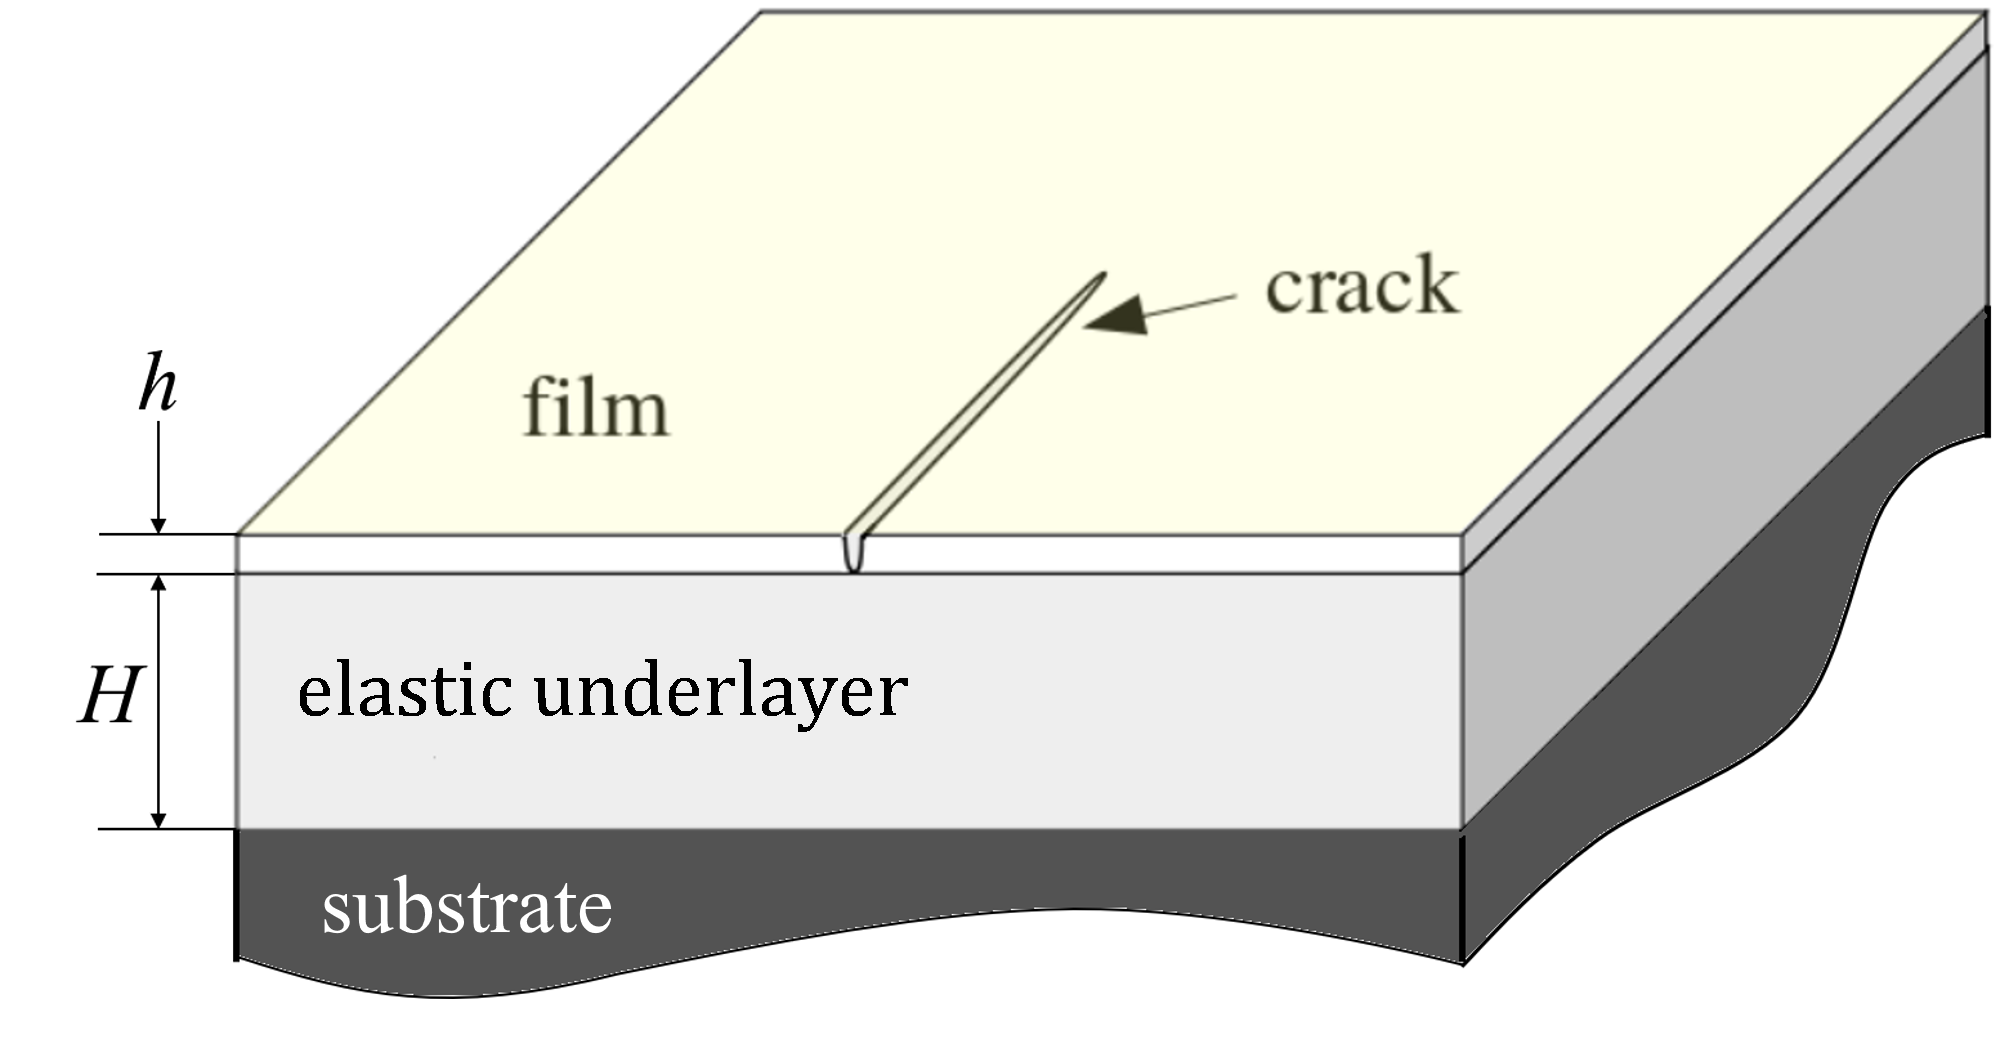
\includegraphics[width=\textwidth,scale=0.5]{Chapter4/figures/2D/top_view.png}
    \caption{}
  \end{subfigure}
  \hspace{0.1\textwidth}
  \begin{subfigure}[b]{0.3\textwidth}
    \centering
    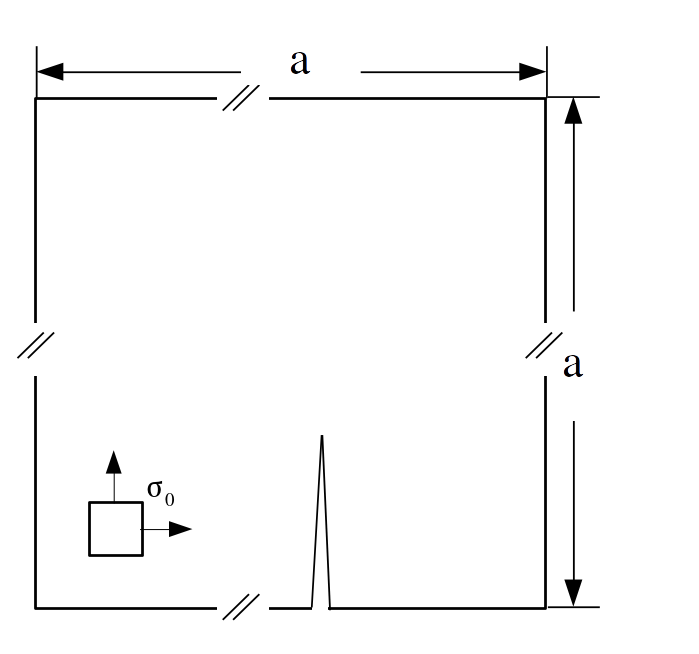
\includegraphics[width=\textwidth,scale=0.5]{Chapter4/figures/2D/2D_schematic.png}
    \caption{}
  \end{subfigure}
  \caption[Description of a two-dimensional model for thin-film cracking.]{Description of a two-dimensional model for thin-film cracking. (a) Top view (highlighted in yellow) (b) schematic representation of the top view. A typical crack is shown to emphasize that fracture is only considered in the film. }
  \label{fig: Chapter4/2D/simplification}
\end{figure}


We consider a square domain and assume the characteristic fragment sizes to be small compared to the overall specimen dimensions, and impose periodic boundary conditions on all four boundaries. Assuming the underlying elastic layer is sufficiently thick and that the shear stress is uniform, equilibrium of a differential element of the film at the film-layer interface yields
\begin{align}
  \grad \cdot \stress = \mu \dfrac{\bs{u}}{hH} ,
\end{align}
where $\stress = \mathbb{C}:[\strain - \mathbb{S}:(\sigma_0\bs{I})]$ is the stress, $\mu$ is the shear modulus of the elastic underlayer, and $\bs{u}$ is the displacement. The corresponding potential energy representing the mismatch between the two sides of the film-layer interface can be written as
\begin{align}
  \psi_{\text{interface}} = \dfrac{1}{2}\dfrac{\mu}{hH}\norm{\bs{u}}^2 .
\end{align}
The underlying elastic layer is assumed to be much thicker than the film, i.e.\ $H = mh$, where $m \gg 1$. The interfacial energy can therefore be simplified as
\begin{align}
  \psi_{\text{interface}} = \dfrac{1}{2}\dfrac{\mu}{mh^2}\norm{\bs{u}}^2.
\end{align}
The total energy of the simplified plane-stress model can then be written as
\begin{equation}
  \begin{split}
    \Psi_\total = &\ -\underbrace{\left( \int\limits_\bodyboundary \bs{\tau} \cdot \bs{u} \diff{A} + \int\limits_\body \bs{b} \cdot \bs{u} \diff{V} \right)}_{\text{external energy}} + \underbrace{\int\limits_\body g(d)\psi_\elastic^\activepart \diff{V} + \int\limits_\body\psi_\elastic^\inactivepart \diff{V}}_{\text{degraded elastic energy}} \\
    &\ + \underbrace{\int\limits_\body g(d)\dfrac{1}{2}\dfrac{\mu}{mh^2}\norm{\bs{u}}^2 \diff{V}}_{\text{degraded interfacial energy}} + \underbrace{\int\limits_\body \dfrac{3\mathcal{G}_c}{8l} \left( d + l^2 \norm{\grad d}^2 \right) \diff{V}}_{\text{approx. fracture energy}}
  \end{split}
\end{equation}
For all calculations in \Cref{s: Chapter4/2D}, we assume $\dfrac{\mu}{mh^2} = 0.1$.

The square domain is discretized using linear triangular elements with a characteristic length of $h^e = a/500$. This  mesh is used for the displacement subproblem for linear elasticity, the phase-field subproblem for fracture, and the generalized eigenvalue problem for the random fields. The displacement field and the damage field are constrained to be $a-$periodic, and the random fields are constructed to be $a-$periodic as well.

%%%%%%%%%%%%%%%%%%%%%%%%%%%%%%%%%%%%%%%%%%%%%%%%%%%%%%%%%%%%%%%%%%%%%%%%%%%%%%%%%%%%%%%%%%%
%%%%%%%%%%%%%%%%%%%%%%%%%%%%%%%%%%%%%%%%%%%%%%%%%%%%%%%%%%%%%%%%%%%%%%%%%%%%%%%%%%%%%%%%%%%
%%%%%%%%%%%%%%%%%%%%%%%%%%%%%%%%%%%%%%%%%%%%%%%%%%%%%%%%%%%%%%%%%%%%%%%%%%%%%%%%%%%%%%%%%%%
%%%%%%%%%%%%%%%%%%%%%%%%%%%%%%%%%%%%%%%%%%%%%%%%%%%%%%%%%%%%%%%%%%%%%%%%%%%%%%%%%%%%%%%%%%%
%%%%%%%%%%%%%%%%%%%%%%%%%%%%%%%%%%%%%%%%%%%%%%%%%%%%%%%%%%%%%%%%%%%%%%%%%%%%%%%%%%%%%%%%%%%
%%%%%%%%%%%%%%%%%%%%%%%%%%%%%%%%%%%%%%%%%%%%%%%%%%%%%%%%%%%%%%%%%%%%%%%%%%%%%%%%%%%%%%%%%%%
%%%%%%%%%%%%%%%%%%%%%%%%%%%%%%%%%%%%%%%%%%%%%%%%%%%%%%%%%%%%%%%%%%%%%%%%%%%%%%%%%%%%%%%%%%%
%%%%%%%%%%%%%%%%%%%%%%%%%%%%%%%%%%%%%%%%%%%%%%%%%%%%%%%%%%%%%%%%%%%%%%%%%%%%%%%%%%%%%%%%%%%
%%%%%%%%%%%%%%%%%%%%%%%%%%%%%%%%%%%%%%%%%%%%%%%%%%%%%%%%%%%%%%%%%%%%%%%%%%%%%%%%%%%%%%%%%%%
%%%%%%%%%%%%%%%%%%%%%%%%%%%%%%%%%%%%%%%%%%%%%%%%%%%%%%%%%%%%%%%%%%%%%%%%%%%%%%%%%%%%%%%%%%%
\subsubsection{Effect of Correlation Length and Smoothness}

To study the effect of the correlation length, crack patterns for four different values of $L$ are compared. Ten calculations, corresponding to ten samples of the stochastic fields, are carried out for each value of $L$. Representative random fields and their corresponding damage fields are shown in \Cref{fig: Chapter4/2D/compare_correlation_length}. A Flooding algorithm (described in \Cref{s: appendix/flooding}) is used to group elements into clusters in a volume-preserving way, to facilitate the counting of distinct fragments. Following the one-dimensional derivation (\Cref{s: application/1D}), two dimensionless parameters are extracted as
\begin{align}
   & \mathcal{D}^* = \sqrt{\dfrac{(1-\nu_1^2)h}{E_1\underline{\mathcal{G}_c}}}\sigma_0, \quad l^* = \dfrac{\lambda}{h}, \quad \lambda \approx \sqrt{A} ,
\end{align}
where the crack spacing $\lambda$ is estimated from the fragment area $A$. Dimensionless curves are plotted in \Cref{fig: Chapter4/2D/statistics_correlation_length}.

As expected, it is seen that the PSE covariance model generates smoother realizations. As the normalized correlation length $L^* = L/p$ becomes larger, i.e.\ \Cref{fig: Chapter4/2D/d_sqexp_cartesian_5_5_rho_0_seed_a,fig: Chapter4/2D/d_sqexp_cartesian_10_10_rho_0_seed_a,fig: Chapter4/2D/d_sqexp_cartesian_20_20_rho_0_seed_a},
a substantial amount of damage accumulates before localization occurs to form a ``crack''. When the sample exhibits less spatial fluctuations, a non-negligible portion of the energy is dissipated into the matrix in the form of diffuse damage, resulting in fewer cracks and larger fragment sizes. As the normalized correlation gets even larger, i.e.\ \Cref{fig: Chapter4/2D/Gc_sqexp_cartesian_20_20_rho_0_seed_a,fig: Chapter4/2D/psic_sqexp_cartesian_20_20_rho_0_seed_a,fig: Chapter4/2D/d_sqexp_cartesian_20_20_rho_0_seed_a}, morphologically different crack networks are obtained.

On the other hand, the rougher samples generated using the PE covariance function, i.e.\ \Cref{fig: Chapter4/2D/Gc_exp_cartesian_5_5_rho_0_seed_b,fig: Chapter4/2D/psic_exp_cartesian_5_5_rho_0_seed_b,fig: Chapter4/2D/d_exp_cartesian_5_5_rho_0_seed_b,fig: Chapter4/2D/Gc_exp_cartesian_10_10_rho_0_seed_b,fig: Chapter4/2D/psic_exp_cartesian_10_10_rho_0_seed_b,fig: Chapter4/2D/d_exp_cartesian_10_10_rho_0_seed_b,fig: Chapter4/2D/Gc_exp_cartesian_20_20_rho_0_seed_b,fig: Chapter4/2D/psic_exp_cartesian_20_20_rho_0_seed_b,fig: Chapter4/2D/d_exp_cartesian_20_20_rho_0_seed_b}, have sufficient variations that serve as effective imperfections for damage localization. In terms of the mean size of fragments that form, the corresponding damage fields are seen to be far less sensitive to the spatial correlation length.  However, as the correlation length increases, the orientation of the damage fields begins to acquire a structure that aligns with the axes of the domain. This observation is in accordance with the tensor-product structure of the covariance model, and with the fact that larger correlation lengths allow more pronounced spatial structures to develop (sample-wise) for PE functions.

Samples obtained with the two covariance models (parameterized by the same correlation lengths), considering the same realization for the underlying Gaussian field (from one covariance model to another), are compared in \Cref{fig: Chapter4/2D/compare_smoothness} to study the effect of smoothness. It is seen that rougher material properties provide more candidate locations for damage localization, hence resulting in more fragments per unit volume of the domain (in a statistical sense). More precisely, the probability density functions (PDFs) corresponding to the dimensionless crack spacing (\Cref{fig: Chapter4/2D/statistics_smoothness}), estimated using approximately 2000 fragments and 10 independent realizations of the fields, show a substantial difference:the mean fragment size obtained with rough material properties (here, with the PE model) turns out to be much smaller than the mean fragment size generated by smoother samples of fracture properties (associated with the PSE model).

\begin{figure}[!htbp]
  \centering
  \begin{subfigure}[b]{0.45\textwidth}
    \caption*{Squared Exponential Kernel}
  \end{subfigure}
  \begin{subfigure}[b]{0.45\textwidth}
    \caption*{Exponential Kernel}
  \end{subfigure}
  
  \begin{subfigure}[b]{0.15\textwidth}
    \caption*{$\Gc^*$}
    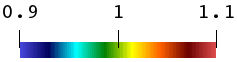
\includegraphics[width=\textwidth]{Chapter4/figures/rainbow_horizontal.png}
  \end{subfigure}
  \begin{subfigure}[b]{0.15\textwidth}
    \caption*{$\psi_c^*$}
    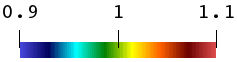
\includegraphics[width=\textwidth]{Chapter4/figures/rainbow_horizontal.png}
  \end{subfigure}
  \begin{subfigure}[b]{0.15\textwidth}
    \caption*{$d$}
    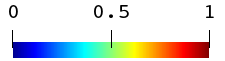
\includegraphics[width=\textwidth]{Chapter4/figures/jet_horizontal.png}
  \end{subfigure}
  \begin{subfigure}[b]{0.15\textwidth}
    \caption*{$\Gc^*$}
    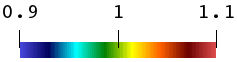
\includegraphics[width=\textwidth]{Chapter4/figures/rainbow_horizontal.png}
  \end{subfigure}
  \begin{subfigure}[b]{0.15\textwidth}
    \caption*{$\psi_c^*$}
    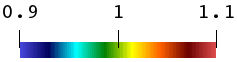
\includegraphics[width=\textwidth]{Chapter4/figures/rainbow_horizontal.png}
  \end{subfigure}
  \begin{subfigure}[b]{0.15\textwidth}
    \caption*{$d$}
    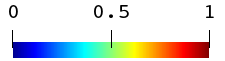
\includegraphics[width=\textwidth]{Chapter4/figures/jet_horizontal.png}
  \end{subfigure}
  
  \begin{subfigure}[b]{0.15\textwidth}
    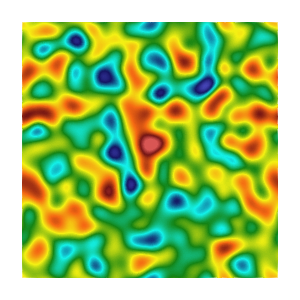
\includegraphics[width=\textwidth]{Chapter4/figures/2D/Gc_sqexp_cartesian_5_5_rho_0_seed_a.png}
    \caption{$L^* = 0.05$}
    \label{fig: Chapter4/2D/Gc_sqexp_cartesian_5_5_rho_0_seed_a}
  \end{subfigure}
  \begin{subfigure}[b]{0.15\textwidth}
    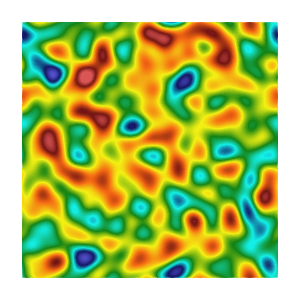
\includegraphics[width=\textwidth]{Chapter4/figures/2D/psic_sqexp_cartesian_5_5_rho_0_seed_a.png}
    \caption{$L^* = 0.05$}
    \label{fig: Chapter4/2D/psic_sqexp_cartesian_5_5_rho_0_seed_a}
  \end{subfigure}
  \begin{subfigure}[b]{0.15\textwidth}
    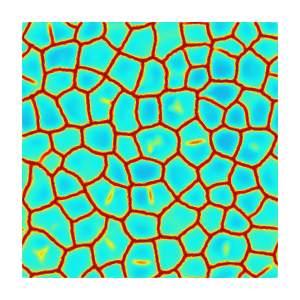
\includegraphics[width=\textwidth]{Chapter4/figures/2D/d_sqexp_cartesian_5_5_rho_0_seed_a.png}
    \caption{}
    \label{fig: Chapter4/2D/d_sqexp_cartesian_5_5_rho_0_seed_a}
  \end{subfigure}
  \begin{subfigure}[b]{0.15\textwidth}
    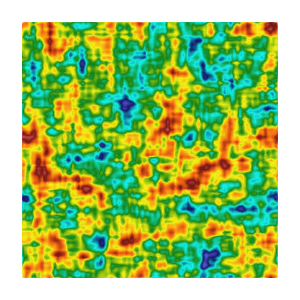
\includegraphics[width=\textwidth]{Chapter4/figures/2D/Gc_exp_cartesian_5_5_rho_0_seed_b.png}
    \caption{$L^* = 0.05$}
    \label{fig: Chapter4/2D/Gc_exp_cartesian_5_5_rho_0_seed_b}
  \end{subfigure}
  \begin{subfigure}[b]{0.15\textwidth}
    \includegraphics[width=\textwidth]{Chapter4/figures/2D/psic_exp_cartesian_5_5_rho_0_seed_b.png}
    \caption{$L^* = 0.05$}
    \label{fig: Chapter4/2D/psic_exp_cartesian_5_5_rho_0_seed_b}
  \end{subfigure}
  \begin{subfigure}[b]{0.15\textwidth}
    \includegraphics[width=\textwidth]{Chapter4/figures/2D/d_exp_cartesian_5_5_rho_0_seed_b.png}
    \caption{}
    \label{fig: Chapter4/2D/d_exp_cartesian_5_5_rho_0_seed_b}
  \end{subfigure}
  
  \begin{subfigure}[b]{0.15\textwidth}
    \includegraphics[width=\textwidth]{Chapter4/figures/2D/Gc_sqexp_cartesian_10_10_rho_0_seed_a.png}
    \caption{$L^* = 0.1$}
    \label{fig: Chapter4/2D/Gc_sqexp_cartesian_10_10_rho_0_seed_a}
  \end{subfigure}
  \begin{subfigure}[b]{0.15\textwidth}
    \includegraphics[width=\textwidth]{Chapter4/figures/2D/psic_sqexp_cartesian_10_10_rho_0_seed_a.png}
    \caption{$L^* = 0.1$}
    \label{fig: Chapter4/2D/psic_sqexp_cartesian_10_10_rho_0_seed_a}
  \end{subfigure}
  \begin{subfigure}[b]{0.15\textwidth}
    \includegraphics[width=\textwidth]{Chapter4/figures/2D/d_sqexp_cartesian_10_10_rho_0_seed_a.png}
    \caption{}
    \label{fig: Chapter4/2D/d_sqexp_cartesian_10_10_rho_0_seed_a}
  \end{subfigure}
  \begin{subfigure}[b]{0.15\textwidth}
    \includegraphics[width=\textwidth]{Chapter4/figures/2D/Gc_exp_cartesian_10_10_rho_0_seed_b.png}
    \caption{$L^* = 0.1$}
    \label{fig: Chapter4/2D/Gc_exp_cartesian_10_10_rho_0_seed_b}
  \end{subfigure}
  \begin{subfigure}[b]{0.15\textwidth}
    \includegraphics[width=\textwidth]{Chapter4/figures/2D/psic_exp_cartesian_10_10_rho_0_seed_b.png}
    \caption{$L^* = 0.1$}
    \label{fig: Chapter4/2D/psic_exp_cartesian_10_10_rho_0_seed_b}
  \end{subfigure}
  \begin{subfigure}[b]{0.15\textwidth}
    \includegraphics[width=\textwidth]{Chapter4/figures/2D/d_exp_cartesian_10_10_rho_0_seed_b.png}
    \caption{}
    \label{fig: Chapter4/2D/d_exp_cartesian_10_10_rho_0_seed_b}
  \end{subfigure}
  
  \begin{subfigure}[b]{0.15\textwidth}
    \includegraphics[width=\textwidth]{Chapter4/figures/2D/Gc_sqexp_cartesian_20_20_rho_0_seed_a.png}
    \caption{$L^* = 0.2$}
    \label{fig: Chapter4/2D/Gc_sqexp_cartesian_20_20_rho_0_seed_a}
  \end{subfigure}
  \begin{subfigure}[b]{0.15\textwidth}
    \includegraphics[width=\textwidth]{Chapter4/figures/2D/psic_sqexp_cartesian_20_20_rho_0_seed_a.png}
    \caption{$L^* = 0.2$}
    \label{fig: Chapter4/2D/psic_sqexp_cartesian_20_20_rho_0_seed_a}
  \end{subfigure}
  \begin{subfigure}[b]{0.15\textwidth}
    \includegraphics[width=\textwidth]{Chapter4/figures/2D/d_sqexp_cartesian_20_20_rho_0_seed_a.png}
    \caption{}
    \label{fig: Chapter4/2D/d_sqexp_cartesian_20_20_rho_0_seed_a}
  \end{subfigure}
  \begin{subfigure}[b]{0.15\textwidth}
    \includegraphics[width=\textwidth]{Chapter4/figures/2D/Gc_exp_cartesian_20_20_rho_0_seed_b.png}
    \caption{$L^* = 0.2$}
    \label{fig: Chapter4/2D/Gc_exp_cartesian_20_20_rho_0_seed_b}
  \end{subfigure}
  \begin{subfigure}[b]{0.15\textwidth}
    \includegraphics[width=\textwidth]{Chapter4/figures/2D/psic_exp_cartesian_20_20_rho_0_seed_b.png}
    \caption{$L^* = 0.2$}
    \label{fig: Chapter4/2D/psic_exp_cartesian_20_20_rho_0_seed_b}
  \end{subfigure}
  \begin{subfigure}[b]{0.15\textwidth}
    \includegraphics[width=\textwidth]{Chapter4/figures/2D/d_exp_cartesian_20_20_rho_0_seed_b.png}
    \caption{}
    \label{fig: Chapter4/2D/d_exp_cartesian_20_20_rho_0_seed_b}
  \end{subfigure}
  \caption[Phase fields resulting from six pairs of realizations with different correlation models and normalized correlation lengths.]{Phase fields resulting from six pairs of realizations with different correlation models and normalized correlation lengths. The left three pairs (a-b, g-h, m-n) are realizations obtained with a PSE covariance function, while the right three pairs (d-e, j-k, p-q) are samples generated with a PE covariance function. Energy release rate $\Gc$ and the critical fracture energy $\psi_c$ have a coefficient of variation of $0.03$, and normalized spatial correlation length $L^*$ of (a-b, d-e) $0.05$ (g-h, j-k) $0.1$ (m-n, p-q) $0.2$ The corresponding phase fields are shown in (c, f, i, l, o, r), respectively. In these results, independent realizations of the underlying Gaussian fields are used.}
  \label{fig: Chapter4/2D/compare_correlation_length}
\end{figure}


\begin{figure}[!htb]
  \centering
  \begin{subfigure}[b]{0.45\textwidth}
    \caption*{Squared Exponential Kernel}
  \end{subfigure}
  \begin{subfigure}[b]{0.45\textwidth}
    \caption*{Exponential Kernel}
  \end{subfigure}

  \begin{subfigure}[b]{0.15\textwidth}
    \caption*{$\Gc^*$}
    \includegraphics[width=\textwidth]{Chapter4/figures/rainbow_horizontal.png}
  \end{subfigure}
  \begin{subfigure}[b]{0.15\textwidth}
    \caption*{$\psi_c^*$}
    \includegraphics[width=\textwidth]{Chapter4/figures/rainbow_horizontal.png}
  \end{subfigure}
  \begin{subfigure}[b]{0.15\textwidth}
    \caption*{$d$}
    \includegraphics[width=\textwidth]{Chapter4/figures/jet_horizontal.png}
  \end{subfigure}
  \begin{subfigure}[b]{0.15\textwidth}
    \caption*{$\Gc^*$}
    \includegraphics[width=\textwidth]{Chapter4/figures/rainbow_horizontal.png}
  \end{subfigure}
  \begin{subfigure}[b]{0.15\textwidth}
    \caption*{$\psi_c^*$}
    \includegraphics[width=\textwidth]{Chapter4/figures/rainbow_horizontal.png}
  \end{subfigure}
  \begin{subfigure}[b]{0.15\textwidth}
    \caption*{$d$}
    \includegraphics[width=\textwidth]{Chapter4/figures/jet_horizontal.png}
  \end{subfigure}

  \begin{subfigure}[b]{0.15\textwidth}
    \includegraphics[width=\textwidth]{Chapter4/figures/2D/Gc_sqexp_cartesian_5_5_rho_0_seed_c.png}
    \caption{}
    \label{fig: Chapter4/2D/Gc_sqexp_cartesian_5_5_rho_0_seed_c}
  \end{subfigure}
  \begin{subfigure}[b]{0.15\textwidth}
    \includegraphics[width=\textwidth]{Chapter4/figures/2D/psic_sqexp_cartesian_5_5_rho_0_seed_c.png}
    \caption{}
    \label{fig: Chapter4/2D/psic_sqexp_cartesian_5_5_rho_0_seed_c}
  \end{subfigure}
  \begin{subfigure}[b]{0.15\textwidth}
    \includegraphics[width=\textwidth]{Chapter4/figures/2D/d_sqexp_cartesian_5_5_rho_0_seed_c.png}
    \caption{}
    \label{fig: Chapter4/2D/d_sqexp_cartesian_5_5_rho_0_seed_c}
  \end{subfigure}
  \begin{subfigure}[b]{0.15\textwidth}
    \includegraphics[width=\textwidth]{Chapter4/figures/2D/Gc_exp_cartesian_5_5_rho_0_seed_c.png}
    \caption{}
    \label{fig: Chapter4/2D/Gc_exp_cartesian_5_5_rho_0_seed_c}
  \end{subfigure}
  \begin{subfigure}[b]{0.15\textwidth}
    \includegraphics[width=\textwidth]{Chapter4/figures/2D/psic_exp_cartesian_5_5_rho_0_seed_c.png}
    \caption{}
    \label{fig: Chapter4/2D/psic_exp_cartesian_5_5_rho_0_seed_c}
  \end{subfigure}
  \begin{subfigure}[b]{0.15\textwidth}
    \includegraphics[width=\textwidth]{Chapter4/figures/2D/d_exp_cartesian_5_5_rho_0_seed_c.png}
    \caption{}
    \label{fig: Chapter4/2D/d_exp_cartesian_5_5_rho_0_seed_c}
  \end{subfigure}

  \begin{subfigure}[b]{0.15\textwidth}
    \includegraphics[width=\textwidth]{Chapter4/figures/2D/Gc_sqexp_cartesian_5_5_rho_0_seed_d.png}
    \caption{}
    \label{fig: Chapter4/2D/Gc_sqexp_cartesian_5_5_rho_0_seed_d}
  \end{subfigure}
  \begin{subfigure}[b]{0.15\textwidth}
    \includegraphics[width=\textwidth]{Chapter4/figures/2D/psic_sqexp_cartesian_5_5_rho_0_seed_d.png}
    \caption{}
    \label{fig: Chapter4/2D/psic_sqexp_cartesian_5_5_rho_0_seed_d}
  \end{subfigure}
  \begin{subfigure}[b]{0.15\textwidth}
    \includegraphics[width=\textwidth]{Chapter4/figures/2D/d_sqexp_cartesian_5_5_rho_0_seed_d.png}
    \caption{}
    \label{fig: Chapter4/2D/d_sqexp_cartesian_5_5_rho_0_seed_d}
  \end{subfigure}
  \begin{subfigure}[b]{0.15\textwidth}
    \includegraphics[width=\textwidth]{Chapter4/figures/2D/Gc_exp_cartesian_5_5_rho_0_seed_d.png}
    \caption{}
    \label{fig: Chapter4/2D/Gc_exp_cartesian_5_5_rho_0_seed_d}
  \end{subfigure}
  \begin{subfigure}[b]{0.15\textwidth}
    \includegraphics[width=\textwidth]{Chapter4/figures/2D/psic_exp_cartesian_5_5_rho_0_seed_d.png}
    \caption{}
    \label{fig: Chapter4/2D/psic_exp_cartesian_5_5_rho_0_seed_d}
  \end{subfigure}
  \begin{subfigure}[b]{0.15\textwidth}
    \includegraphics[width=\textwidth]{Chapter4/figures/2D/d_exp_cartesian_5_5_rho_0_seed_d.png}
    \caption{}
    \label{fig: Chapter4/2D/d_exp_cartesian_5_5_rho_0_seed_d}
  \end{subfigure}

  \begin{subfigure}[b]{0.15\textwidth}
    \includegraphics[width=\textwidth]{Chapter4/figures/2D/Gc_sqexp_cartesian_5_5_rho_0_seed_e.png}
    \caption{}
    \label{fig: Chapter4/2D/Gc_sqexp_cartesian_5_5_rho_0_seed_e}
  \end{subfigure}
  \begin{subfigure}[b]{0.15\textwidth}
    \includegraphics[width=\textwidth]{Chapter4/figures/2D/psic_sqexp_cartesian_5_5_rho_0_seed_e.png}
    \caption{}
    \label{fig: Chapter4/2D/psic_sqexp_cartesian_5_5_rho_0_seed_e}
  \end{subfigure}
  \begin{subfigure}[b]{0.15\textwidth}
    \includegraphics[width=\textwidth]{Chapter4/figures/2D/d_sqexp_cartesian_5_5_rho_0_seed_e.png}
    \caption{}
    \label{fig: Chapter4/2D/d_sqexp_cartesian_5_5_rho_0_seed_e}
  \end{subfigure}
  \begin{subfigure}[b]{0.15\textwidth}
    \includegraphics[width=\textwidth]{Chapter4/figures/2D/Gc_exp_cartesian_5_5_rho_0_seed_e.png}
    \caption{}
    \label{fig: Chapter4/2D/Gc_exp_cartesian_5_5_rho_0_seed_e}
  \end{subfigure}
  \begin{subfigure}[b]{0.15\textwidth}
    \includegraphics[width=\textwidth]{Chapter4/figures/2D/psic_exp_cartesian_5_5_rho_0_seed_e.png}
    \caption{}
    \label{fig: Chapter4/2D/psic_exp_cartesian_5_5_rho_0_seed_e}
  \end{subfigure}
  \begin{subfigure}[b]{0.15\textwidth}
    \includegraphics[width=\textwidth]{Chapter4/figures/2D/d_exp_cartesian_5_5_rho_0_seed_e.png}
    \caption{}
    \label{fig: Chapter4/2D/d_exp_cartesian_5_5_rho_0_seed_e}
  \end{subfigure}
  \caption{ Three pairs of qualitative comparison of smoothness of the kernel function with the same normalized  correlation length $L^* = 0.05$. (a-f) pair 1 (g-l) pair 2 (m-r) pair 3. Each row compares two kernel functions transformed from the same samples of the underlying Gaussian fields. }
  \label{fig: Chapter4/2D/compare_smoothness}
\end{figure}


\begin{figure}[htbp!]
  \centering
  \begin{subfigure}[b]{0.475\textwidth}
    \centering
    \tikzsetnextfilenamesafe{Chapter4/2D/dimensionless_curve_correlation_length_sqexp}
    \begin{tikzpicture}
      \begin{axis}[
          width=0.9\textwidth,
          height=1.1\textwidth,
          ymode=log,
          log ticks with fixed point,
          ylabel=$\underline{l^*}$,xlabel=$\mathcal{D}^*$,
          % ymin=0,ymax=2.5,
          legend style={
              at={(0.05,0.05)},
              anchor=south west,
              nodes={scale=1, transform shape},
              fill=none,
              draw=none,
              text opacity=1,
              cells={align=left}
            },
          legend cell align={left},
          every axis plot/.append style={thick}
        ]
        % sqexp l = 5
        \addplot [select coords between index={40}{220},color=black] table [x expr=\thisrowno{0},y expr=\thisrowno{1}]{Chapter4/data/2D/dimensionless_curve_sqexp_cartesian_5_5.csv};
        % sqexp l = 10
        \addplot [select coords between index={40}{220},color=red] table [x expr=\thisrowno{0},y expr=\thisrowno{1}]{Chapter4/data/2D/dimensionless_curve_sqexp_cartesian_10_10.csv};
        % sqexp l = 20
        \addplot [select coords between index={40}{220},color=blue] table [x expr=\thisrowno{0},y expr=\thisrowno{1}]{Chapter4/data/2D/dimensionless_curve_sqexp_cartesian_20_20.csv};
        \legend{sqexp $L^* = 0.05$,sqexp $L^* = 0.1$,sqexp $L^* = 0.2$}
      \end{axis}
    \end{tikzpicture}
    \caption{}
    \label{fig: Chapter4/2D/dimensionless_curve_correlation_length_sqexp}
  \end{subfigure}
  \begin{subfigure}[b]{0.475\textwidth}
    \centering
    \tikzsetnextfilenamesafe{Chapter4/2D/distribution_correlation_length_sqexp}
    \begin{tikzpicture}
      \begin{axis}[
          width=0.9\textwidth,
          height=1.1\textwidth,
          xlabel=$l^*$,ylabel=estimated PDF,
          ymin=0,ymax=0.012,
          xmin=0,xmax=1000,
          legend style={at={(0.95,0.95)},anchor=north east},
          legend style={nodes={scale=1, transform shape}},
          legend style={fill=none,draw=none},
          legend cell align={left},
          every axis plot/.append style={thick}
        ]
        \addplot [color=black] table [x expr=\thisrowno{0},y expr=\thisrowno{1}]{Chapter4/data/2D/distribution_sqexp_cartesian_5_5.csv};
        \addplot [color=red] table [x expr=\thisrowno{0},y expr=\thisrowno{1}]{Chapter4/data/2D/distribution_sqexp_cartesian_10_10.csv};
        \addplot [color=blue] table [x expr=\thisrowno{0},y expr=\thisrowno{1}]{Chapter4/data/2D/distribution_sqexp_cartesian_20_20.csv};
        \legend{sqexp $L^* = 0.05$,sqexp $L^* = 0.1$,sqexp $L^* = 0.2$}
      \end{axis}
    \end{tikzpicture}
    \caption{}
    \label{fig: Chapter4/2D/distribution_correlation_length_sqexp}
  \end{subfigure}
  
  \begin{subfigure}[b]{0.475\textwidth}
    \centering
    \tikzsetnextfilenamesafe{Chapter4/2D/dimensionless_curve_correlation_length_exp}
    \begin{tikzpicture}
      \begin{axis}[
          width=0.9\textwidth,
          height=1.1\textwidth,
          ymode=log,
          log ticks with fixed point,
          ylabel=$\underline{l^*}$,xlabel=$\mathcal{D}^*$,
          % ymin=0,ymax=2.5,
          legend style={
              at={(0.05,0.05)},
              anchor=south west,
              nodes={scale=1, transform shape},
              fill=none,
              draw=none,
              text opacity=1,
              cells={align=left}
            },
          legend cell align={left},
          every axis plot/.append style={thick}
        ]
        % sqexp l = 5
        \addplot [select coords between index={40}{220},color=black] table [x expr=\thisrowno{0},y expr=\thisrowno{1}]{Chapter4/data/2D/dimensionless_curve_exp_cartesian_5_5.csv};
        % sqexp l = 10
        \addplot [select coords between index={40}{220},color=red] table [x expr=\thisrowno{0},y expr=\thisrowno{1}]{Chapter4/data/2D/dimensionless_curve_exp_cartesian_10_10.csv};
        % sqexp l = 20
        \addplot [select coords between index={40}{220},color=blue] table [x expr=\thisrowno{0},y expr=\thisrowno{1}]{Chapter4/data/2D/dimensionless_curve_exp_cartesian_20_20.csv};
        \legend{exp $L^* = 0.05$,exp $L^* = 0.1$,exp $L^* = 0.2$}
      \end{axis}
    \end{tikzpicture}
    \caption{}
    \label{fig: Chapter4/2D/dimensionless_curve_correlation_length_exp}
  \end{subfigure}
  \begin{subfigure}[b]{0.475\textwidth}
    \centering
    \tikzsetnextfilenamesafe{Chapter4/2D/distribution_correlation_length_exp}
    \begin{tikzpicture}
      \begin{axis}[
          width=0.9\textwidth,
          height=1.1\textwidth,
          xlabel=$l^*$,ylabel=estimated PDF,
          ymin=0,ymax=0.012,
          xmin=0,xmax=300,
          legend style={at={(0.95,0.95)},anchor=north east},
          legend style={nodes={scale=1, transform shape}},
          legend style={fill=none,draw=none},
          legend cell align={left},
          every axis plot/.append style={thick}
        ]
        \addplot [color=black] table [x expr=\thisrowno{0},y expr=\thisrowno{1}]{Chapter4/data/2D/distribution_exp_cartesian_5_5.csv};
        \addplot [color=red] table [x expr=\thisrowno{0},y expr=\thisrowno{1}]{Chapter4/data/2D/distribution_exp_cartesian_10_10.csv};
        \addplot [color=blue] table [x expr=\thisrowno{0},y expr=\thisrowno{1}]{Chapter4/data/2D/distribution_exp_cartesian_20_20.csv};
        \legend{exp $L^* = 0.05$,exp $L^* = 0.1$,exp $L^* = 0.2$}
      \end{axis}
    \end{tikzpicture}
    \caption{}
    \label{fig: Chapter4/2D/distribution_correlation_length_exp}
  \end{subfigure}
  \caption[Fragment statistics for different values of correlation length.]{(a, c) Mean dimensionless crack spacing $\underline{l^*}$ versus dimensionless crack driving force $\mathcal{D}^*$ (b, d) Estimated probability density of dimensionless crack spacing for different values of correlation length when $\mathcal{D}^* = 5.17$ based on (a-b) a PSE kernel (c-d) a PE kernel }
  \label{fig: Chapter4/2D/statistics_correlation_length}
\end{figure}


\begin{figure}[htb!]
  \centering
  \begin{subfigure}[b]{0.475\textwidth}
    \centering
    \tikzsetnextfilenamesafe{Chapter4/2D/dimensionless_curve_smoothness}
    \begin{tikzpicture}
      \begin{axis}[
          width=\textwidth,
          height=0.9\textwidth,
          ymode=log,
          log ticks with fixed point,
          ylabel=$\underline{l^*}$,xlabel=$\mathcal{D}^*$,
          % ymin=0,ymax=2.5,
          legend style={
              at={(0.05,0.05)},
              anchor=south west,
              nodes={scale=1, transform shape},
              fill=none,
              draw=none,
              text opacity=1,
              cells={align=left}
            },
          legend cell align={left},
          every axis plot/.append style={thick}
        ]
        % sqexp
        \addplot [select coords between index={40}{220},color=black] table [x expr=\thisrowno{0},y expr=\thisrowno{1}]{Chapter4/data/2D/dimensionless_curve_sqexp_cartesian_5_5.csv};
        % exp
        \addplot [select coords between index={40}{220},color=red] table [x expr=\thisrowno{0},y expr=\thisrowno{1}]{Chapter4/data/2D/dimensionless_curve_exp_cartesian_5_5.csv};
        \legend{sqexp,exp}
      \end{axis}
    \end{tikzpicture}
    \caption{}
    \label{fig: Chapter4/2D/dimensionless_curve_smoothness}
  \end{subfigure}
  \begin{subfigure}[b]{0.475\textwidth}
    \centering
    \tikzsetnextfilenamesafe{hapter4/2D/distribution_smoothness}
    \begin{tikzpicture}
      \begin{axis}[
          width=\textwidth,
          height=0.9\textwidth,
          xlabel=$l^*$,ylabel=estimated PDF,
          ymin=0,ymax=0.012,
          xmin=0,xmax=300,
          legend style={at={(0.95,0.95)},anchor=north east},
          legend style={nodes={scale=1, transform shape}},
          legend style={fill=none, draw=none},
          legend cell align={left},
          every axis plot/.append style={thick}
        ]
        \addplot [color=black] table [x expr=\thisrowno{0},y expr=\thisrowno{1}]{Chapter4/data/2D/distribution_sqexp_cartesian_5_5.csv};
        \addplot [color=red] table [x expr=\thisrowno{0},y expr=\thisrowno{1}]{Chapter4/data/2D/distribution_exp_cartesian_5_5.csv};
        \legend{sqexp,exp}
      \end{axis}
    \end{tikzpicture}
    \caption{}
    \label{fig: Chapter4/2D/distribution_smoothness}
  \end{subfigure}
  \caption[Fragment statistics for different covariance kernels.]{Comparisons of (a) mean dimensionless crack spacing $\underline{l^*}$ versus dimensionless crack driving force $\mathcal{D}^*$ and (b) Estimated probability density of dimensionless crack spacing with the same correlation length when $\mathcal{D}^* = 5.17$ for results obtained using a PSE kernel and a PE kernel}
  \label{fig: Chapter4/2D/statistics_smoothness}
\end{figure}


%%%%%%%%%%%%%%%%%%%%%%%%%%%%%%%%%%%%%%%%%%%%%%%%%%%%%%%%%%%%%%%%%%%%%%%%%%%%%%%%%%%%%%%%%%%
%%%%%%%%%%%%%%%%%%%%%%%%%%%%%%%%%%%%%%%%%%%%%%%%%%%%%%%%%%%%%%%%%%%%%%%%%%%%%%%%%%%%%%%%%%%
%%%%%%%%%%%%%%%%%%%%%%%%%%%%%%%%%%%%%%%%%%%%%%%%%%%%%%%%%%%%%%%%%%%%%%%%%%%%%%%%%%%%%%%%%%%
%%%%%%%%%%%%%%%%%%%%%%%%%%%%%%%%%%%%%%%%%%%%%%%%%%%%%%%%%%%%%%%%%%%%%%%%%%%%%%%%%%%%%%%%%%%
%%%%%%%%%%%%%%%%%%%%%%%%%%%%%%%%%%%%%%%%%%%%%%%%%%%%%%%%%%%%%%%%%%%%%%%%%%%%%%%%%%%%%%%%%%%
%%%%%%%%%%%%%%%%%%%%%%%%%%%%%%%%%%%%%%%%%%%%%%%%%%%%%%%%%%%%%%%%%%%%%%%%%%%%%%%%%%%%%%%%%%%
%%%%%%%%%%%%%%%%%%%%%%%%%%%%%%%%%%%%%%%%%%%%%%%%%%%%%%%%%%%%%%%%%%%%%%%%%%%%%%%%%%%%%%%%%%%
%%%%%%%%%%%%%%%%%%%%%%%%%%%%%%%%%%%%%%%%%%%%%%%%%%%%%%%%%%%%%%%%%%%%%%%%%%%%%%%%%%%%%%%%%%%
%%%%%%%%%%%%%%%%%%%%%%%%%%%%%%%%%%%%%%%%%%%%%%%%%%%%%%%%%%%%%%%%%%%%%%%%%%%%%%%%%%%%%%%%%%%
%%%%%%%%%%%%%%%%%%%%%%%%%%%%%%%%%%%%%%%%%%%%%%%%%%%%%%%%%%%%%%%%%%%%%%%%%%%%%%%%%%%%%%%%%%%
\subsubsection{Parametric Analysis}

The stochastic model constructed in this paper enables the introduction of point-wise correlation (that is, in the first-order marginal probability distribution) between the two fracture properties.
With regard to fracture mechanics, one might wonder, for example, whether or not the fracture toughness $\Gc$ and the critical fracture energy $\psi_c$ are correlated (at a given location), and if so, to what extent. In this section, we perform a parametric analysis for different values of the correlation coefficient $\rho$, with the aim of understanding which field plays a dominant role in determining the resulting fracture morphology in thin films.

In order to obtain meaningful statistical results, 10 independent realizations are considered, and the same samples (of the underlying Gaussian random fields) are used when $\rho$ varies. The normalized correlation length is set to $L^* = 0.05$ for both fracture properties.
Three pairs of fracture toughness and critical fracture energy samples, constructed using \eqref{eq: def-P1} and \eqref{eq: def-P2} with $\rho \in \{0, 0.5, 1\}$, are shown in \Cref{fig: Chapter4/2D/compare_correlation}. Note that the special case of $\rho = 0$ recovers the case of independent material properties.

\begin{figure}[!htb]
  \centering
  \begin{subfigure}[b]{0.42\textwidth}
    \caption*{Squared Exponential Kernel}
  \end{subfigure}
  \begin{subfigure}[b]{0.42\textwidth}
    \caption*{Exponential Kernel}
  \end{subfigure}
  \hspace{0.05\textwidth}

  \begin{subfigure}[b]{0.14\textwidth}
    \caption*{$\rho = 0$}
  \end{subfigure}
  \begin{subfigure}[b]{0.14\textwidth}
    \caption*{$\rho = 0.5$}
  \end{subfigure}
  \begin{subfigure}[b]{0.14\textwidth}
    \caption*{$\rho = 1$}
  \end{subfigure}
  \begin{subfigure}[b]{0.14\textwidth}
    \caption*{$\rho = 0$}
  \end{subfigure}
  \begin{subfigure}[b]{0.14\textwidth}
    \caption*{$\rho = 0.5$}
  \end{subfigure}
  \begin{subfigure}[b]{0.14\textwidth}
    \caption*{$\rho = 1$}
  \end{subfigure}
  \hspace{0.05\textwidth}

  \begin{subfigure}[b]{0.14\textwidth}
    \includegraphics[width=\textwidth]{Chapter4/figures/2D/Gc_sqexp_cartesian_5_5_rho_1_sample_1.png}
    \caption{}
  \end{subfigure}
  \begin{subfigure}[b]{0.14\textwidth}
    \includegraphics[width=\textwidth]{Chapter4/figures/2D/Gc_sqexp_cartesian_5_5_rho_1_sample_1.png}
    \caption{}
  \end{subfigure}
  \begin{subfigure}[b]{0.14\textwidth}
    \includegraphics[width=\textwidth]{Chapter4/figures/2D/Gc_sqexp_cartesian_5_5_rho_1_sample_1.png}
    \caption{}
  \end{subfigure}
  \begin{subfigure}[b]{0.14\textwidth}
    \includegraphics[width=\textwidth]{Chapter4/figures/2D/Gc_exp_cartesian_5_5_rho_1_sample_1.png}
    \caption{}
  \end{subfigure}
  \begin{subfigure}[b]{0.14\textwidth}
    \includegraphics[width=\textwidth]{Chapter4/figures/2D/Gc_exp_cartesian_5_5_rho_1_sample_1.png}
    \caption{}
  \end{subfigure}
  \begin{subfigure}[b]{0.14\textwidth}
    \includegraphics[width=\textwidth]{Chapter4/figures/2D/Gc_exp_cartesian_5_5_rho_1_sample_1.png}
    \caption{}
  \end{subfigure}
  \begin{subfigure}[b]{0.05\textwidth}
    \caption*{$\Gc^*$}
    \includegraphics[width=\textwidth]{Chapter4/figures/rainbow_vertical.png}
    \vspace{0.05in}
  \end{subfigure}

  \begin{subfigure}[b]{0.14\textwidth}
    \includegraphics[width=\textwidth]{Chapter4/figures/2D/psic_sqexp_cartesian_5_5_rho_0_sample_1.png}
    \caption{}
  \end{subfigure}
  \begin{subfigure}[b]{0.14\textwidth}
    \includegraphics[width=\textwidth]{Chapter4/figures/2D/psic_sqexp_cartesian_5_5_rho_0_5_sample_1.png}
    \caption{}
  \end{subfigure}
  \begin{subfigure}[b]{0.14\textwidth}
    \includegraphics[width=\textwidth]{Chapter4/figures/2D/psic_sqexp_cartesian_5_5_rho_1_sample_1.png}
    \caption{}
  \end{subfigure}
  \begin{subfigure}[b]{0.14\textwidth}
    \includegraphics[width=\textwidth]{Chapter4/figures/2D/psic_exp_cartesian_5_5_rho_0_sample_1.png}
    \caption{}
  \end{subfigure}
  \begin{subfigure}[b]{0.14\textwidth}
    \includegraphics[width=\textwidth]{Chapter4/figures/2D/psic_exp_cartesian_5_5_rho_0_5_sample_1.png}
    \caption{}
  \end{subfigure}
  \begin{subfigure}[b]{0.14\textwidth}
    \includegraphics[width=\textwidth]{Chapter4/figures/2D/psic_exp_cartesian_5_5_rho_1_sample_1.png}
    \caption{}
  \end{subfigure}
  \begin{subfigure}[b]{0.05\textwidth}
    \caption*{$\psi_c^*$}
    \includegraphics[width=\textwidth]{Chapter4/figures/rainbow_vertical.png}
    \vspace{0.05in}
  \end{subfigure}
  \caption{ Point-wise correlated material properties: (a-f) normalized fracture toughness $\Gc^*$ and (g-l) normalized critical fracture energy $\psi_c^*$ with (left) PSE covariance function (right) PE covariance function }
  \label{fig: Chapter4/2D/compare_correlation}
\end{figure}


Statistics of the dimensionless crack spacing $l^*$ are once again extracted at $\mathcal{D}^* = 5.17$. The resulting dimensionless curves and normalized probability density functions are shown in \Cref{fig: Chapter4/2D/statistics_sensitivity_sqexp,fig: Chapter4/2D/statistics_sensitivity_exp}. These results indicate that the distribution of fragment size is relatively insensitive to the coefficient of correlation, regardless of the smoothness of the covariance kernel.

\begin{figure}[htb!]
  \centering
  \begin{subfigure}[b]{0.475\textwidth}
    \centering
    \tikzsetnextfilenamesafe{Chapter4/2D/statistics_sensitivity_sqexp/dimensionless_curve}
    \begin{tikzpicture}
      \begin{axis}[
          width=\textwidth,
          height=0.9\textwidth,
          ymode=log,
          log ticks with fixed point,
          ylabel=$\underline{l^*}$,xlabel=$\mathcal{D}^*$,
          % ymin=0,ymax=2.5,
          legend style={
              at={(0.05,0.05)},
              anchor=south west,
              nodes={scale=1, transform shape},
              fill=white,
              fill opacity=0.8,
              draw opacity=1,
              text opacity=1,
              cells={align=left}
            },
          legend cell align={left},
          every axis plot/.append style={thick}
        ]
        % rho = 0
        \addplot [select coords between index={40}{220},color=black] table [x expr=\thisrowno{0},y expr=\thisrowno{1}]{Chapter4/data/2D/dimensionless_curve_sqexp_rho_1.csv};
        % rho = 0.5
        \addplot [select coords between index={40}{220},color=red] table [x expr=\thisrowno{0},y expr=\thisrowno{1}]{Chapter4/data/2D/dimensionless_curve_sqexp_rho_2.csv};
        % rho = 1
        \addplot [select coords between index={40}{220},color=blue] table [x expr=\thisrowno{0},y expr=\thisrowno{1}]{Chapter4/data/2D/dimensionless_curve_sqexp_rho_3.csv};
        \legend{$\rho=0$,$\rho=0.5$,$\rho=1$}
      \end{axis}
    \end{tikzpicture}
    \caption{}
  \end{subfigure}
  \begin{subfigure}[b]{0.475\textwidth}
    \centering
    \tikzsetnextfilenamesafe{Chapter4/2D/statistics_sensitivity_sqexp/distribution}
    \begin{tikzpicture}
      \begin{axis}[
          width=\textwidth,
          height=0.9\textwidth,
          xlabel=$l^*$,ylabel=estimated PDF,
          ymin=0,ymax=0.012,
          xmin=0,xmax=300,
          legend style={at={(0.95,0.95)},anchor=north east},
          legend style={nodes={scale=1, transform shape}},
          legend cell align={left},
          every axis plot/.append style={thick}
        ]
        \addplot [color=black] table [x expr=\thisrowno{0},y expr=\thisrowno{1}]{Chapter4/data/2D/distribution_sqexp_rho_1.csv};
        \addplot [color=red] table [x expr=\thisrowno{0},y expr=\thisrowno{1}]{Chapter4/data/2D/distribution_sqexp_rho_2.csv};
        \addplot [color=blue] table [x expr=\thisrowno{0},y expr=\thisrowno{1}]{Chapter4/data/2D/distribution_sqexp_rho_3.csv};
        \legend{$\rho=0$,$\rho=0.5$,$\rho=1$}
      \end{axis}
    \end{tikzpicture}
    \caption{}
  \end{subfigure}
  \caption{Comparisons of (a) mean dimensionless crack spacing as a function of dimensionless crack driving force and (b) estimated PDFs of dimensionless fragment size at loading $\mathcal{D}^* = 5.17$ for results with an underlying PSE kernel}
  \label{fig: Chapter4/2D/statistics_sensitivity_sqexp}
\end{figure}

\begin{figure}[htb!]
  \centering
  \begin{subfigure}[b]{0.475\textwidth}
    \centering
    \tikzsetnextfilenamesafe{Chapter4/2D/statistics_sensitivity_exp/dimensionless_curve}
    \begin{tikzpicture}
      \begin{axis}[
          width=\textwidth,
          height=0.9\textwidth,
          ymode=log,
          log ticks with fixed point,
          ylabel=$\underline{l^*}$,xlabel=$\mathcal{D}^*$,
          % ymin=0,ymax=2.5,
          legend style={
              at={(0.05,0.05)},
              anchor=south west,
              nodes={scale=1, transform shape},
              fill=white,
              fill opacity=0.8,
              draw opacity=1,
              text opacity=1,
              cells={align=left}
            },
          legend cell align={left},
          every axis plot/.append style={thick}
        ]
        % rho = 0
        \addplot [select coords between index={40}{220},color=black] table [x expr=\thisrowno{0},y expr=\thisrowno{1}]{Chapter4/data/2D/dimensionless_curve_exp_rho_1.csv};
        % rho = 0.5
        \addplot [select coords between index={40}{220},color=red] table [x expr=\thisrowno{0},y expr=\thisrowno{1}]{Chapter4/data/2D/dimensionless_curve_exp_rho_2.csv};
        % rho = 1
        \addplot [select coords between index={40}{220},color=blue] table [x expr=\thisrowno{0},y expr=\thisrowno{1}]{Chapter4/data/2D/dimensionless_curve_exp_rho_3.csv};
        \legend{$\rho=0$,$\rho=0.5$,$\rho=1$}
      \end{axis}
    \end{tikzpicture}
    \caption{}
  \end{subfigure}
  \begin{subfigure}[b]{0.475\textwidth}
    \centering
    \tikzsetnextfilenamesafe{Chapter4/2D/statistics_sensitivity_exp/distribution}
    \begin{tikzpicture}
      \begin{axis}[
          width=\textwidth,
          height=0.9\textwidth,
          xlabel=$l^*$,ylabel=estimated PDF,
          ymin=0,ymax=0.012,
          xmin=0,xmax=300,
          legend style={at={(0.95,0.95)},anchor=north east},
          legend style={nodes={scale=1, transform shape}},
          legend cell align={left},
          every axis plot/.append style={thick}
        ]
        \addplot [color=black] table [x expr=\thisrowno{0},y expr=\thisrowno{1}]{Chapter4/data/2D/distribution_exp_rho_1.csv};
        \addplot [color=red] table [x expr=\thisrowno{0},y expr=\thisrowno{1}]{Chapter4/data/2D/distribution_exp_rho_2.csv};
        \addplot [color=blue] table [x expr=\thisrowno{0},y expr=\thisrowno{1}]{Chapter4/data/2D/distribution_exp_rho_3.csv};
        \legend{$\rho=0$,$\rho=0.5$,$\rho=1$}
      \end{axis}
    \end{tikzpicture}
    \caption{}
  \end{subfigure}
  \caption{Comparisons of (a) mean dimensionless crack spacing and dimensionless crack driving force and (b) estimated PDFs of dimensionless fragment size at loading $\mathcal{D}^* = 5.17$ for results with an underlying PE kernel}
  \label{fig: Chapter4/2D/statistics_sensitivity_exp}
\end{figure}


In contrast, when we superimpose the fracture patterns, we observe that the fracture morphology does exhibit a sensitivity to variations in the fracture toughness  (\Cref{fig: Chapter4/2D/morphology_psic_constant}). The superimposed results are only shown for the PSE covariance function, but comparable results are obtained with the PE covariance function.
By comparison, when the fracture toughness is held fixed while the critical fracture energy is varied, the superimposed fracture patterns are nearly indistinguishable (\Cref{fig: Chapter4/2D/morphology_Gc_constant}). The clear conclusion is that the energetics are primarily responsible for driving the fracture morphology, a result that is not surprising. This conclusion is also supported by the results shown in \Cref{fig: Chapter4/2D/compare_sensitivity_sqexp,fig: Chapter4/2D/compare_sensitivity_exp}, in which fracture patterns are plotted over contours of the fracture toughness and the critical energy. For both types of covariance functions, the fracture patterns are seen to follow contours of minimal fracture toughness while largely ignoring those of the critical fracture energy.

% !TEX root = ../../../main.tex

\begin{figure}[!htbp]
  \centering
  \begin{subfigure}[b]{0.4\textwidth}
    \includegraphics[width=\textwidth]{Chapter4/figures/2D/psic_constant.png}
    \caption{}
    \label{fig: Chapter4/2D/morphology_psic_constant}
  \end{subfigure}
  \begin{subfigure}[b]{0.4\textwidth}
    \includegraphics[width=\textwidth]{Chapter4/figures/2D/Gc_constant.png}
    \caption{}
    \label{fig: Chapter4/2D/morphology_Gc_constant}
  \end{subfigure}
  \begin{subfigure}[b]{0.1\textwidth}
    \includegraphics[width=\textwidth]{Chapter4/figures/rho.png}
    \caption*{}
    \vspace{0.75in}
  \end{subfigure}
  \caption[Superposition of fracture networks obtained by three samples of different coefficients of correlation, using the PSE kernel.]{ Superposition of fracture networks obtained by three samples of different coefficients of correlation, using the PSE kernel. Only the volume within the damage contour of $d = 0.9$ is shown to represent the resulting fracture network. Three samples are sampled (a) by holding $\Gc$ constant and (b) by holding $\psi_c$ constant. }
  \label{fig: Chapter4/2D/compare_morphology}
\end{figure}


\begin{figure}[!htbp]
  \centering
  \begin{subfigure}[b]{0.25\textwidth}
    \includegraphics[width=\textwidth]{Chapter4/figures/2D/Gc_sqexp_cartesian_5_5_rho_0_seed_a_with_crack_140.png}
    \caption{$\mathcal{D}^* = 3.06$}
    \label{fig: Chapter4/2D/Gc_sqexp_cartesian_5_5_rho_0_seed_a_with_crack_140}
  \end{subfigure}
  \begin{subfigure}[b]{0.25\textwidth}
    \includegraphics[width=\textwidth]{Chapter4/figures/2D/Gc_sqexp_cartesian_5_5_rho_0_seed_a_with_crack_160.png}
    \caption{$\mathcal{D}^* = 3.76$}
    \label{fig: Chapter4/2D/Gc_sqexp_cartesian_5_5_rho_0_seed_a_with_crack_160}
  \end{subfigure}
  \begin{subfigure}[b]{0.25\textwidth}
    \includegraphics[width=\textwidth]{Chapter4/figures/2D/Gc_sqexp_cartesian_5_5_rho_0_seed_a_with_crack_220.png}
    \caption{$\mathcal{D}^* = 5.17$}
    \label{fig: Chapter4/2D/Gc_sqexp_cartesian_5_5_rho_0_seed_a_with_crack_220}
  \end{subfigure}
  \begin{subfigure}[b]{0.08\textwidth}
    \caption*{$\Gc^*$}
    \includegraphics[width=\textwidth]{Chapter4/figures/rainbow_vertical.png}
    \vspace{0.15in}
  \end{subfigure}
  
  \begin{subfigure}[b]{0.25\textwidth}
    \includegraphics[width=\textwidth]{Chapter4/figures/2D/psic_sqexp_cartesian_5_5_rho_0_seed_a_with_crack_140.png}
    \caption{$\mathcal{D}^* = 3.06$}
    \label{fig: Chapter4/2D/psic_sqexp_cartesian_5_5_rho_0_seed_a_with_crack_140}
  \end{subfigure}
  \begin{subfigure}[b]{0.25\textwidth}
    \includegraphics[width=\textwidth]{Chapter4/figures/2D/psic_sqexp_cartesian_5_5_rho_0_seed_a_with_crack_160.png}
    \caption{$\mathcal{D}^* = 3.76$}
    \label{fig: Chapter4/2D/psic_sqexp_cartesian_5_5_rho_0_seed_a_with_crack_160}
  \end{subfigure}
  \begin{subfigure}[b]{0.25\textwidth}
    \includegraphics[width=\textwidth]{Chapter4/figures/2D/psic_sqexp_cartesian_5_5_rho_0_seed_a_with_crack_220.png}
    \caption{$\mathcal{D}^* = 5.17$}
    \label{fig: Chapter4/2D/psic_sqexp_cartesian_5_5_rho_0_seed_a_with_crack_220}
  \end{subfigure}
  \begin{subfigure}[b]{0.08\textwidth}
    \caption*{$\psi_c^*$}
    \includegraphics[width=\textwidth]{Chapter4/figures/rainbow_vertical.png}
    \vspace{0.15in}
  \end{subfigure}
  \caption[Snapshots of phase field at different loading levels with a PSE covariance function.]{Snapshots of phase field at different loading levels with $d \geqslant 0.75$ plotted over (a-c) fracture toughness $\Gc$ and (d-f) critical fracture energy $\psi_c$ with an underlying PSE covariance function }
  \label{fig: Chapter4/2D/compare_sensitivity_sqexp}
\end{figure}

\begin{figure}[!htbp]
  \centering
  \begin{subfigure}[b]{0.25\textwidth}
    \includegraphics[width=\textwidth]{Chapter4/figures/2D/Gc_exp_cartesian_5_5_rho_0_seed_b_with_crack_140.png}
    \caption{$\mathcal{D}^* = 3.06$}
    \label{fig: Chapter4/2D/Gc_exp_cartesian_5_5_rho_0_seed_a_with_crack_140}
  \end{subfigure}
  \begin{subfigure}[b]{0.25\textwidth}
    \includegraphics[width=\textwidth]{Chapter4/figures/2D/Gc_exp_cartesian_5_5_rho_0_seed_b_with_crack_160.png}
    \caption{$\mathcal{D}^* = 3.76$}
    \label{fig: Chapter4/2D/Gc_exp_cartesian_5_5_rho_0_seed_a_with_crack_160}
  \end{subfigure}
  \begin{subfigure}[b]{0.25\textwidth}
    \includegraphics[width=\textwidth]{Chapter4/figures/2D/Gc_exp_cartesian_5_5_rho_0_seed_b_with_crack_220.png}
    \caption{$\mathcal{D}^* = 5.17$}
    \label{fig: Chapter4/2D/Gc_exp_cartesian_5_5_rho_0_seed_a_with_crack_220}
  \end{subfigure}
  \begin{subfigure}[b]{0.08\textwidth}
    \caption*{$\Gc^*$}
    \includegraphics[width=\textwidth]{Chapter4/figures/rainbow_vertical.png}
    \vspace{0.15in}
  \end{subfigure}
  
  \begin{subfigure}[b]{0.25\textwidth}
    \includegraphics[width=\textwidth]{Chapter4/figures/2D/psic_exp_cartesian_5_5_rho_0_seed_b_with_crack_140.png}
    \caption{$\mathcal{D}^* = 3.06$}
    \label{fig: Chapter4/2D/psic_exp_cartesian_5_5_rho_0_seed_a_with_crack_140}
  \end{subfigure}
  \begin{subfigure}[b]{0.25\textwidth}
    \includegraphics[width=\textwidth]{Chapter4/figures/2D/psic_exp_cartesian_5_5_rho_0_seed_b_with_crack_160.png}
    \caption{$\mathcal{D}^* = 3.76$}
    \label{fig: Chapter4/2D/psic_exp_cartesian_5_5_rho_0_seed_a_with_crack_160}
  \end{subfigure}
  \begin{subfigure}[b]{0.25\textwidth}
    \includegraphics[width=\textwidth]{Chapter4/figures/2D/psic_exp_cartesian_5_5_rho_0_seed_b_with_crack_220.png}
    \caption{$\mathcal{D}^* = 5.17$}
    \label{fig: Chapter4/2D/psic_exp_cartesian_5_5_rho_0_seed_a_with_crack_220}
  \end{subfigure}
  \begin{subfigure}[b]{0.08\textwidth}
    \caption*{$\psi_c^*$}
    \includegraphics[width=\textwidth]{Chapter4/figures/rainbow_vertical.png}
    \vspace{0.15in}
  \end{subfigure}
  \caption[Snapshots of phase field at different loading levels with a PE covariance function.]{Snapshots of phase field at different loading levels with $d \geqslant 0.75$ plotted over (a-c) fracture toughness $\Gc$ and (d-f) critical fracture energy $\psi_c$ with an underlying PE covariance function }
  \label{fig: Chapter4/2D/compare_sensitivity_exp}
\end{figure}


%%%%%%%%%%%%%%%%%%%%%%%%%%%%%%%%%%%%%%%%%%%%%%%%%%%%%%%%%%%%%%%%%%%%%%%%%%%%%%%%%%%%%%%%%%%
%%%%%%%%%%%%%%%%%%%%%%%%%%%%%%%%%%%%%%%%%%%%%%%%%%%%%%%%%%%%%%%%%%%%%%%%%%%%%%%%%%%%%%%%%%%
%%%%%%%%%%%%%%%%%%%%%%%%%%%%%%%%%%%%%%%%%%%%%%%%%%%%%%%%%%%%%%%%%%%%%%%%%%%%%%%%%%%%%%%%%%%
%%%%%%%%%%%%%%%%%%%%%%%%%%%%%%%%%%%%%%%%%%%%%%%%%%%%%%%%%%%%%%%%%%%%%%%%%%%%%%%%%%%%%%%%%%%
%%%%%%%%%%%%%%%%%%%%%%%%%%%%%%%%%%%%%%%%%%%%%%%%%%%%%%%%%%%%%%%%%%%%%%%%%%%%%%%%%%%%%%%%%%%
%%%%%%%%%%%%%%%%%%%%%%%%%%%%%%%%%%%%%%%%%%%%%%%%%%%%%%%%%%%%%%%%%%%%%%%%%%%%%%%%%%%%%%%%%%%
%%%%%%%%%%%%%%%%%%%%%%%%%%%%%%%%%%%%%%%%%%%%%%%%%%%%%%%%%%%%%%%%%%%%%%%%%%%%%%%%%%%%%%%%%%%
%%%%%%%%%%%%%%%%%%%%%%%%%%%%%%%%%%%%%%%%%%%%%%%%%%%%%%%%%%%%%%%%%%%%%%%%%%%%%%%%%%%%%%%%%%%
%%%%%%%%%%%%%%%%%%%%%%%%%%%%%%%%%%%%%%%%%%%%%%%%%%%%%%%%%%%%%%%%%%%%%%%%%%%%%%%%%%%%%%%%%%%
%%%%%%%%%%%%%%%%%%%%%%%%%%%%%%%%%%%%%%%%%%%%%%%%%%%%%%%%%%%%%%%%%%%%%%%%%%%%%%%%%%%%%%%%%%%
\subsubsection{Discussion on Modeling Flexibility: Impact of the Covariance Structure}

We now briefly examine how different structures of the covariance kernel can alter the fragment morphology. It has been demonstrated experimentally \cite{kitsunezaki2016shaking, kitsunezaki2017stress, halasz2017effect, kitsunezaki2017memory, nakahara2018mechanism}
how macro-scale processing conditions to construct samples may lead to morphologically different crack networks.  For example, \citet{kitsunezaki2017memory} carried out a series of tests to study the effect of macroscopic disturbances on crack patterns. They poured calcium carbonate (CaCO$_3$) paste into a shallow circular container. Different modes of agitation were applied to the paste before it was dried, and the resulting crack patterns showed a strong correlation with the modes of agitation.

We hypothesize that the agitation gives rise to effective fracture properties at the macro-scale that have a structure that is consistent with the agitation. We further assume a rougher spatial variation of properties in the direction parallel to the agitation than in the direction orthogonal to the agitation. Accordingly, we model the spatial variations in the fracture properties using composite covariance functions, defined on purpose by a tensor-product structure involving PSE and PE functions. In Figure \ref{fig: Chapter4/2D/japanese_experiments}, we compare the experimentally-observed crack patterns to our simulation results obtained using random fracture properties with the postulated anisotropic covariance functions. The comparison shows reasonable agreement (without specifically optimizing the  hyperparameters in the stochastic model), indicating that the differing processing conditions may have resulted in different spatial variations in the effective fracture properties.

\begin{figure}[htb!]
  \centering
  \begin{subfigure}{0.14\textwidth}
    \caption*{Mode of agitation}
  \end{subfigure}
  \hspace{0.02\textwidth}
  \begin{subfigure}{0.14\textwidth}
    \caption*{\protect\raggedright Experimental crack network}
  \end{subfigure}
  \hspace{0.02\textwidth}
  \begin{subfigure}{0.15\textwidth}
    \caption*{$\Gc^*$}
    \includegraphics[width=\textwidth]{Chapter4/figures/rainbow_horizontal.png}
  \end{subfigure}
  \begin{subfigure}{0.15\textwidth}
    \caption*{$\psi_c^*$}
    \includegraphics[width=\textwidth]{Chapter4/figures/rainbow_horizontal.png}
  \end{subfigure}
  \begin{subfigure}{0.15\textwidth}
    \caption*{$d$}
    \includegraphics[width=\textwidth]{Chapter4/figures/grayscale_horizontal.png}
  \end{subfigure}
  
  \begin{subfigure}{0.14\textwidth}
    \includegraphics[width=\textwidth]{Chapter4/figures/2D/brick_schematic.png}
    \caption{}
  \end{subfigure}
  \hspace{0.02\textwidth}
  \begin{subfigure}{0.14\textwidth}
    \includegraphics[width=\textwidth]{Chapter4/figures/2D/paste_brick.png}
    \caption{}
  \end{subfigure}
  \hspace{0.02\textwidth}
  \begin{subfigure}{0.15\textwidth}
    \includegraphics[width=\textwidth]{Chapter4/figures/2D/Gc_brick.png}
    \caption{}
  \end{subfigure}
  \begin{subfigure}{0.15\textwidth}
    \includegraphics[width=\textwidth]{Chapter4/figures/2D/psic_brick.png}
    \caption{}
  \end{subfigure}
  \begin{subfigure}{0.15\textwidth}
    \includegraphics[width=\textwidth]{Chapter4/figures/2D/d_brick.png}
    \caption{}
  \end{subfigure}
  
  \begin{subfigure}{0.14\textwidth}
    \includegraphics[width=\textwidth]{Chapter4/figures/2D/radial_schematic.png}
    \caption{}
  \end{subfigure}
  \hspace{0.02\textwidth}
  \begin{subfigure}{0.14\textwidth}
    \includegraphics[width=\textwidth]{Chapter4/figures/2D/paste_radial.png}
    \caption{}
  \end{subfigure}
  \hspace{0.02\textwidth}
  \begin{subfigure}{0.15\textwidth}
    \includegraphics[width=\textwidth]{Chapter4/figures/2D/Gc_radial.png}
    \caption{}
  \end{subfigure}
  \begin{subfigure}{0.15\textwidth}
    \includegraphics[width=\textwidth]{Chapter4/figures/2D/psic_radial.png}
    \caption{}
  \end{subfigure}
  \begin{subfigure}{0.15\textwidth}
    \includegraphics[width=\textwidth]{Chapter4/figures/2D/d_radial.png}
    \caption{}
  \end{subfigure}
  
  \begin{subfigure}{0.14\textwidth}
    \includegraphics[width=\textwidth]{Chapter4/figures/2D/ring_schematic.png}
    \caption{}
  \end{subfigure}
  \hspace{0.02\textwidth}
  \begin{subfigure}{0.14\textwidth}
    \includegraphics[width=\textwidth]{Chapter4/figures/2D/paste_ring.png}
    \caption{}
  \end{subfigure}
  \hspace{0.02\textwidth}
  \begin{subfigure}{0.15\textwidth}
    \includegraphics[width=\textwidth]{Chapter4/figures/2D/Gc_ring.png}
    \caption{}
  \end{subfigure}
  \begin{subfigure}{0.15\textwidth}
    \includegraphics[width=\textwidth]{Chapter4/figures/2D/psic_ring.png}
    \caption{}
  \end{subfigure}
  \begin{subfigure}{0.15\textwidth}
    \includegraphics[width=\textwidth]{Chapter4/figures/2D/d_ring.png}
    \caption{}
  \end{subfigure}
  \caption[Three sets of experiments and calculations with different modes of agitation.]{Three sets of experiments and calculations for (a-e) unilateral agitation (f-j) rotational agitation (k-o) point agitation. (b, g, l) snapshots of crack patterns from experiments. postulated spatially correlated (c, h, m) fracture toughness and (d, i, n) critical fracture energy to reproduce experimental observations. (e, j, o) phase fields obtained using corresponding spatially varying material properties. }
  \label{fig: Chapter4/2D/japanese_experiments}
\end{figure}


%%%%%%%%%%%%%%%%%%%%%%%%%%%%%%%%%%%%%%%%%%%%%%%%%%%%%%%%%%%%%%%%%%%%%%%%%%%%%%%%%%%%%%%%%%%
%%%%%%%%%%%%%%%%%%%%%%%%%%%%%%%%%%%%%%%%%%%%%%%%%%%%%%%%%%%%%%%%%%%%%%%%%%%%%%%%%%%%%%%%%%%
%%%%%%%%%%%%%%%%%%%%%%%%%%%%%%%%%%%%%%%%%%%%%%%%%%%%%%%%%%%%%%%%%%%%%%%%%%%%%%%%%%%%%%%%%%%
%%%%%%%%%%%%%%%%%%%%%%%%%%%%%%%%%%%%%%%%%%%%%%%%%%%%%%%%%%%%%%%%%%%%%%%%%%%%%%%%%%%%%%%%%%%
%%%%%%%%%%%%%%%%%%%%%%%%%%%%%%%%%%%%%%%%%%%%%%%%%%%%%%%%%%%%%%%%%%%%%%%%%%%%%%%%%%%%%%%%%%%
%%%%%%%%%%%%%%%%%%%%%%%%%%%%%%%%%%%%%%%%%%%%%%%%%%%%%%%%%%%%%%%%%%%%%%%%%%%%%%%%%%%%%%%%%%%
%%%%%%%%%%%%%%%%%%%%%%%%%%%%%%%%%%%%%%%%%%%%%%%%%%%%%%%%%%%%%%%%%%%%%%%%%%%%%%%%%%%%%%%%%%%
%%%%%%%%%%%%%%%%%%%%%%%%%%%%%%%%%%%%%%%%%%%%%%%%%%%%%%%%%%%%%%%%%%%%%%%%%%%%%%%%%%%%%%%%%%%
%%%%%%%%%%%%%%%%%%%%%%%%%%%%%%%%%%%%%%%%%%%%%%%%%%%%%%%%%%%%%%%%%%%%%%%%%%%%%%%%%%%%%%%%%%%
%%%%%%%%%%%%%%%%%%%%%%%%%%%%%%%%%%%%%%%%%%%%%%%%%%%%%%%%%%%%%%%%%%%%%%%%%%%%%%%%%%%%%%%%%%%
\subsection{Inverse Identification Based on Three-Dimensional Physical Experiments}

In \citet{Rodriguez2006}, a series of drying tests with mining waste placed on grooved circular plates (\SI{225}{\milli\meter} in diameter) was performed to observe crack evolution due to desiccation processes. Three tests were carried out with different film thicknesses $h \in \{ \SI{4}{\milli\meter}, \SI{8}{\milli\meter}, \text{and}~\SI{16}{\milli\meter} \}$.

\begin{table}[htb!]
  \centering
  \caption{Summary of material properties of mining waste and model parameters for all calculations in \Cref{s: Chapter4/3D}}
  \begin{tabular}{r c c c c}
    \toprule
    Property/Parameter            & Symbol                      & Value & Unit                                & Comment                                                     \\
    \midrule
    Young's modulus               & $E$                         & 4     & \SI{}{\mega\pascal}                 & See \cite{sanchez2014modeling}                              \\
    Poisson's ratio               & $\nu$                       & 0.2   & nondim.                             & See \cite{sanchez2014modeling}                              \\
    Mean fracture toughness       & $\underline{\mathcal{G}_c}$ & 27    & \SI{}{\kilo\joule\per\square\meter} & See \cite{rodriguez2007experimental,lakshmikantha2009image} \\[5pt]
    Mean critical fracture energy & $\underline{\psi_c}$        & 30    & \SI{}{\joule\per\square\meter}      & See \cite{rodriguez2007experimental,lakshmikantha2009image} \\[5pt]
    Regularization length         & $l$                         & 0.8   & \SI{}{\milli\meter}                 & Such that $2l/h^e \approx 5$                                \\
    Degradation shape parameter   & $p$                         & 1     & nondim.                             &                                                             \\
    \bottomrule
  \end{tabular}
  \label{tab: MW}
\end{table}

\begin{figure}
  \centering
  \begin{overpic}[scale=0.55]{Chapter4/figures/3D/inverse.png}
    \put(4,-4){\footnotesize\textbf{(a)}}
    \put(32,-4){\footnotesize\textbf{(b)}}
    \put(57,-4){\footnotesize\textbf{(c)}}
    \put(89,-4){\footnotesize\textbf{(d)}}
  \end{overpic}
  \vspace{0.2in}
  \caption[Procedures of finding the optimal hyperparameter to match the experiment.]{Procedures of finding the optimal hyperparameter to match the experiment: (a)  12 pairs of fracture properties are sampled to explore the space of admissible spatial correlation lengths; three dimensional energy minimization problems are solved to obtain (b) the resulting fracture morphology; (c) distributions of fragment sizes are extracted from the simulated results, and the log-likelihood values of these distributions at the samples extracted from (d) the experimental fracture morphology are computed.}
  \label{fig: Chapter4/3D/inverse}
\end{figure}


To replicate this study using model-based simulations and our phase-field model (enhanced with the stochastic description of fracture properties), we adopt fully three-dimensional models.  The material properties used for this study are  listed in \Cref{tab: MW}.  Consistent with the experimental studies of \cite{Rodriguez2006}, the film-substrate system is represented by a cylindrical domain. The substrate is modeled as a rigid body with an arbitrarily high fracture toughness. The substrate and film are discretized using tetrahedral elements with characteristic lengths of $h^e_0 = \SI{1.6}{\milli\meter}$ and $h^e_1 = \SI{0.36}{\milli\meter}$, respectively. The solutions to the linear elasticity subproblem, the phase-field for fracture subproblem, and the generalized eigenvalue problem are once again approximated using the same mesh.

We first calibrate the spatial variability in our model against the experimental observations of the fracture patterns for the thinnest ($h = 4$mm) specimen. To formulate the statistical inverse problem, we assume that (1) the fracture toughness and the critical fracture energy are uncorrelated (i.e., $\rho = 0$); and (2) both fracture properties have the same coefficient of variation (set to 0.03) and spatial correlation lengths, and that they can be defined using isotropic squared exponential kernels. In addition, the variations of the properties through the thickness of the film are assumed negligible compared to in-plane variations.

Based on these assumptions, the spatial correlation length $L$ is the only parameter to be determined, and a parametric search is performed in $\mathbb{L} = \{$ \SI{3}{\milli\meter}, \SI{3.5}{\milli\meter}, \SI{4}{\milli\meter}, \SI{4.5}{\milli\meter}, \SI{5}{\milli\meter}, \SI{5.5}{\milli\meter}, \SI{6}{\milli\meter}, \SI{6.5}{\milli\meter}, \SI{7}{\milli\meter}, \SI{7.5}{\milli\meter}, \SI{8}{\milli\meter}, \SI{8.5}{\milli\meter} $\}$. Energy minimization problems for the case of $h = \SI{4}{\milli\meter}$ are simulated for each pair of realizations and the corresponding fracture patterns are obtained. For a given value of $L \in \mathbb{L}$, the flooding algorithm is used to identify fragments on the top surface of the thin film, and a kernel density estimation of the probability density function associated with the fragment size, denoted by $f_\text{fs}^\text{sim}(\cdot; L)$, is obtained. The optimal value of $L$ is then identified by maximizing the log-likelihood function $\mathcal{L}$ defined as
\begin{align}
  \mathcal{L}(L) = \sum_{A_\text{fs}^\text{exp} \in \mathbb{A}^\text{exp}} \ln{f_\text{fs}^\text{sim}(l^*(A_\text{fs}^\text{exp}); L)}~, \quad l^*(A) = \dfrac{\sqrt{A}}{h}~,
\end{align}
where $\mathbb{A}^\text{exp}$ denotes the collection of fragment size samples extracted by using the same flooding algorithm on the experimental result.
The aforementioned workflow to calibrate the model is summarized in \Cref{fig: Chapter4/3D/inverse}. The fracture properties with spatial correlation $L = \SI{4}{\milli\meter}$ lead to the maximum log-likelihood among the span of samples considered. \Cref{fig: Chapter4/3D/calibrated} compares the estimated PDF and the fracture morphology obtained using the calibrated stochastic model to those of the experimental specimen for $h = \SI{4}{\milli\meter}$.

\begin{figure}[!htbp]
  \centering
  \begin{subfigure}[b]{0.4\textwidth}
    \centering
    \tikzsetnextfilenamesafe{Chapter4/3D/calibrated/pdf}
    \begin{tikzpicture}
      \begin{axis}[
          width=\textwidth,
          height=1\textwidth,
          xlabel=$l^*$,ylabel=estimated PDF,
          ymin=0,ymax=0.5,
          xmin=0,xmax=15,
          legend style={at={(0.95,0.95)},anchor=north east},
          legend style={nodes={scale=1, transform shape}},
          legend style={fill=none, draw=none},
          legend cell align={left},
          every axis plot/.append style={thick}
        ]
        \addplot [color=black] table [x expr=\thisrowno{0},y expr=\thisrowno{1}]{Chapter4/data/3D/calibrated_pdf.csv};
        \addplot [color=red] table [x expr=\thisrowno{0},y expr=\thisrowno{2}]{Chapter4/data/3D/calibrated_pdf.csv};
        \legend{experiment,simulation}
      \end{axis}
    \end{tikzpicture}
    \caption{}
  \end{subfigure}
  \begin{subfigure}[b]{0.27\textwidth}
    \centering
    \includegraphics[width=\textwidth]{Chapter4/figures/3D/d_4.png}
    \vspace{10pt}
    \caption{}
  \end{subfigure}
  \begin{subfigure}[b]{0.25\textwidth}
    \centering
    \includegraphics[width=\textwidth]{Chapter4/figures/3D/4mm_exp.png}
    \vspace{12pt}
    \caption{}
  \end{subfigure}
  \caption{(a) Estimated PDFs of the dimensionless fragment sizes extracted from the experimental result and the calibrated stochastic model. (b) Fracture morphology obtained using the calibrated fracture properties. (c) Photograph of cracks in the mining waste. }
  \label{fig: Chapter4/3D/calibrated}
\end{figure}


To then benchmark our model against specimens with different thicknesses, three 3D calculations are carried out using the same realization of fracture properties with $L = \SI{4}{\milli\meter}$. As shown in \Cref{fig: Chapter4/3D/3D},
our results appear to agree reasonably well with the experimental observations. In general, the thicker films fracture into larger fragments, which also agrees with the simplified models presented in \Cref{s: application/1D,s: application/2D}.

\begin{figure}[!htb]
  \centering
  \begin{subfigure}{0.23\textwidth}
    \includegraphics[width=\textwidth,scale=0.5]{Chapter4/figures/3D/4mm_exp.png}
    \caption{}
  \end{subfigure}
  \hspace{0.05\textwidth}
  \begin{subfigure}{0.23\textwidth}
    \includegraphics[width=\textwidth,scale=0.5]{Chapter4/figures/3D/8mm_exp.png}
    \caption{}
  \end{subfigure}
  \hspace{0.05\textwidth}
  \begin{subfigure}{0.23\textwidth}
    \includegraphics[width=\textwidth,scale=0.5]{Chapter4/figures/3D/16mm_exp.png}
    \caption{}
  \end{subfigure}
  
  \begin{subfigure}{0.23\textwidth}
    \includegraphics[width=\textwidth,scale=0.5]{Chapter4/figures/3D/4mm_top.png}
    \caption{}
  \end{subfigure}
  \hspace{0.05\textwidth}
  \begin{subfigure}{0.23\textwidth}
    \includegraphics[width=\textwidth,scale=0.5]{Chapter4/figures/3D/8mm_top.png}
    \caption{}
  \end{subfigure}
  \hspace{0.05\textwidth}
  \begin{subfigure}{0.23\textwidth}
    \includegraphics[width=\textwidth,scale=0.5]{Chapter4/figures/3D/16mm_top.png}
    \caption{}
  \end{subfigure}
  
  \begin{subfigure}{0.23\textwidth}
    \includegraphics[width=\textwidth,scale=0.5]{Chapter4/figures/3D/4mm_3D.png}
    \caption{}
  \end{subfigure}
  \hspace{0.05\textwidth}
  \begin{subfigure}{0.23\textwidth}
    \includegraphics[width=\textwidth,scale=0.5]{Chapter4/figures/3D/8mm_3D.png}
    \caption{}
  \end{subfigure}
  \hspace{0.05\textwidth}
  \begin{subfigure}{0.23\textwidth}
    \includegraphics[width=\textwidth,scale=0.5]{Chapter4/figures/3D/16mm_3D.png}
    \caption{}
  \end{subfigure}
  \caption[Qualitative comparison between the experiments and the simulations with different thickness.]{Qualitative comparison between the experiments and the simulations: (a-c) Photographs (modified from \cite{Rodriguez2006}) of  cracks in mining waste due to desiccation at steady state for three test specimens with thickness (a) \SI{4}{\milli\meter}, (b) \SI{8}{\milli\meter}, and (c) \SI{16}{\milli\meter}.  (d-f) Top view and (g-i) panoramic view of corresponding numerical simulation results with different film thickness.  Volumes of material with $d \geqslant 0.75$ were removed to improve the visualization of the crack geometry. }
  \label{fig: Chapter4/3D/3D}
\end{figure}



\chapter{Towards Ductile Fracture}
\label{chapter: ductile}

\section{Introduction}
\label{section: ductile/intro}

%extension to plasticity

The thermodynamic framework employed by the phase-field approach provides a convenient extension to incorporate plasticity by incorporating a plastic energy. However, how to best design the form of that plastic energy and its coupling with a phase field that regularizes a fracture surface remains an open question.
There exist many approaches to modeling plasticity in the context of phase-field fracture \cite{alessi_gradient_2014, alessi_gradient_2015, alessi_coupling_2018, ambati_phase-field_2015, ambati_phase-field_2016, miehe_phase_2016, borden_phase-field_2016, borden_phase-field_2017}.  For a recent review of the various approaches that have been proposed, see  \citet{alessi_comparison_2017}. In this chapter, we explore possible extensions to ductile fracture within the proposed variational framework \Cref{section: Chapter2}. The proposed framework is flexible in the sense that a wide range of plastic flow rules and hardening behavior can be cast in a variational setting, as illustrated in \cite{ortiz_variational_1999}.  The consistent variational approach does impart certain restrictions, such as the degradation of the yield surface with the phase field implying a corresponding plastic contribution to crack growth.  While other models that break the variational structure may be of utility to effectively capture certain responses, they are beyond the scope of the current work.

%modeling choices

By adopting such a variational framework to model ductile fracture, the remaining major modeling choices are the form of the local term in the fracture energy (the crack geometric function)\footnote{Also sometimes referred to as the \textit{local fracture dissipation function} in the phase-field for fracture related literature, despite its energetic nature in the thermodynamic framework.}, the plastic degradation function (the functional dependence of the plastic energy on the phase-field variable), and the power expenditure. \citet{pham2013onset} used a crack geometric function that is linear in the phase-field variable, resulting in a purely elastic response prior to crack initiation.  This fracture energy functional was subsequently referred to as the \texttt{AT-1} functional by Bourdin and co-workers (meant to evoke \textit{Ambrosio} and \textit{Tortorelli}, who initially introduced this and related functionals in the context of image segmentation \cite{ambrosio1990approximation}). \citet{wu2017unified} generalized the \textit{Ambrosio-Tortorelli} functional \cite{ambrosio1990approximation} to a family of second-order polynomials with various phase-field profiles, with specific choices of recovering the widely adopted \texttt{AT-1} and \texttt{AT-2} models. In this chapter, we extend the results to the regime of ductile fracture and demonstrate that an unperturbed elastic-plastic response can be obtained in certain cases, i.e.\ the yield stress and the plastic hardening law remain unmodified prior to crack initiation even when the plastic energy is degraded as a function of the phase-field variable.

%properties of Lorentz

In the case of brittle and quasi-brittle fracture, several studies have demonstrated that a regularization-length independent critical fracture strength and softening response can be obtained by a family of rational degradation functions in combination with the appropriate choice of the crack geometric function \cite{lorentz2011convergence, wu2017unified, geelen2019phase}. These are referred to as Lorentz-type degradation functions hereinafter.  In another work \cite{brandon2020cohesive}, we showed that this decoupling of critical fracture strength and regularization length is crucial in elastic-plastic materials to ensure the crack growth resistance is convergent with respect to the regularization. This independence or lack of sensitivity is important both in the study of the $\Gamma$-convergence of the model behavior and in engineering applications where the specimen used for calibration and the actual structure of interest span vastly different spatial scales. In this manuscript, we extend the use of these degradation functions to the coupling of the plastic energy so that the model response converges as the phase-field regularization length diminishes.

Although the phase-field regularization length can be divorced from the set of material properties by choosing the Lorentz-type degradation functions, an upper bound still exists, stemming from either polyconvexity requirements or physical constraints (see e.g. \cite{wu2017unified, geelen2019phase} for detailed analysis). With regard to phase-field models for ductile fracture, various choices of the coupling between damage and plasticity can result in the need for surprisingly small regularization lengths.  In particular, some models require the need for smaller regularization lengths as the transition from plastic localization to the onset of damage is delayed.
There have been several attempts to address this issue. \citet{ambati_phase-field_2015,ambati_phase-field_2016} scaled the plastic degradation function by a critical plastic strain to be calibrated. \citet{miehe2015phase} introduced barrier functions related to critical values of the state variables. Most recently, \citet{borden_phase-field_2016} devised a threshold for the plastic work contributions to crack initiation. Although these are all valid, thermodynamically consistent approaches to introduce an arbitrary delay to crack initiation, the hybrid nature of these formulations makes it difficult to fit them into a variational framework.

Coupling the phase field to the plasticity tends to promote cracks in regions of extensive plasticity, which is often the case observed experimentally, but the observed damage process resulting from the model can be far more gradual than expected. On the other hand, when the phase field is coupled only to the elastic strain energy, the damage process is more abrupt, but the predicted crack growth directions tend not to agree with observations in ductile alloys.  In particular, they tend to propagate orthogonally to the maximum tensile stress as in brittle materials, rather than in response to intense plastic straining. Here, we have identified a plausible micro-mechanical argument to reconcile these problems, and used this to formulate a model that fractures in regions with large plastic deformation even without the strong coupling between plasticity and fracture. Motivated by findings from several recent attempts to homogenize the fracture toughness, in this work we decouple the plastic disspation from fracture degradation and propose a novel coalescence dissipation to model the coupling between plasticity and fracture. \citet{rodriguez2016silica}, \citet{chowdhury2019effects}, and \citet{vo2020molecular} found that ligament length, shape, and orientation of defects at the micro-scale influence the Mode-I fracture toughness. We postulate that the presence of plastic flow (or dislocations at the micro-scale) alters those properties related to defects, and at the continuum level, some configurational energy has been dissipated prior to crack initiation, effectively reducing the fracture toughness. We note that the idea of degrading the fracture toughness is not necessarily new, as a similar approach was recently proposed by \citet{yin2020ductile}. Importantly, by virtue of considering the coalescence dissipation in a variational framework, we show that fracture occurs in regions with large plastic deformation even without the strong coupling between plasticity and fracture.  An upshot is a significant reduction in the fracture driving energy and a corresponding relaxation of the upper bound for the regularization length.

% This paper is organized as follows: \Cref{s: theory} outlines the variational framework. \Cref{s: theory/potential} describes a specific form of the functional to be minimized. \Cref{s: theory/minimizer} describes the minimization problem and the resulting governing equations and constitutive constraints. \Cref{s: theory/discretization} presents the initial boundary value problem, the strong form, the weak form and the discrete Galerkin form.
% \Cref{s: example/homogenized} motivates the choices of the crack geometric function and the degradation function by examining a homogeneous problem in detail. \Cref{s: example/nonhomogeneous} demonstrates the regularization-length-independent softening behavior as well as the effect of the coalescence dissipation term. \Cref{s: example/3pb} applies the proposed model to simulate a three-point bending problem, and \Cref{s: example/SFC} presents simulation results for a recent Sandia Fracture Challenge problem. Finally, \Cref{s: conclusion} provides a summary and some concluding remarks.


\section{Theory}
\label{section: ductile/theory}

%%%%%%%%%%%%%%%%%%%%%%%%%%%%%%%%%%%%%%%%%%%%%%%%%%%%%%%%%%%%%%%%%%%%%%%%%%%%%%%%%%%%%%%%%%%
%%%%%%%%%%%%%%%%%%%%%%%%%%%%%%%%%%%%%%%%%%%%%%%%%%%%%%%%%%%%%%%%%%%%%%%%%%%%%%%%%%%%%%%%%%%
%%%%%%%%%%%%%%%%%%%%%%%%%%%%%%%%%%%%%%%%%%%%%%%%%%%%%%%%%%%%%%%%%%%%%%%%%%%%%%%%%%%%%%%%%%%
%%%%%%%%%%%%%%%%%%%%%%%%%%%%%%%%%%%%%%%%%%%%%%%%%%%%%%%%%%%%%%%%%%%%%%%%%%%%%%%%%%%%%%%%%%%
%%%%%%%%%%%%%%%%%%%%%%%%%%%%%%%%%%%%%%%%%%%%%%%%%%%%%%%%%%%%%%%%%%%%%%%%%%%%%%%%%%%%%%%%%%%
%%%%%%%%%%%%%%%%%%%%%%%%%%%%%%%%%%%%%%%%%%%%%%%%%%%%%%%%%%%%%%%%%%%%%%%%%%%%%%%%%%%%%%%%%%%
%%%%%%%%%%%%%%%%%%%%%%%%%%%%%%%%%%%%%%%%%%%%%%%%%%%%%%%%%%%%%%%%%%%%%%%%%%%%%%%%%%%%%%%%%%%
%%%%%%%%%%%%%%%%%%%%%%%%%%%%%%%%%%%%%%%%%%%%%%%%%%%%%%%%%%%%%%%%%%%%%%%%%%%%%%%%%%%%%%%%%%%
%%%%%%%%%%%%%%%%%%%%%%%%%%%%%%%%%%%%%%%%%%%%%%%%%%%%%%%%%%%%%%%%%%%%%%%%%%%%%%%%%%%%%%%%%%%
%%%%%%%%%%%%%%%%%%%%%%%%%%%%%%%%%%%%%%%%%%%%%%%%%%%%%%%%%%%%%%%%%%%%%%%%%%%%%%%%%%%%%%%%%%%
\subsection{Constitutive choices}

Following the variational framework (\Cref{chapter: framework}), the Helmholtz free energy density is decomposed as
\begin{align}
  \psi = \psi^e + \psi^p + \psi^f, \label{eq: chapter 5 helmholtz}
\end{align}
where $\psi^e$, $\psi^p$ and $\psi^f$ are the strain-energy density, plastic energy density, and fracture energy density, respectively. The strain-energy density for large deformation and the plastic energy density, along with the flow rule constraints and their thermodynamic conjugates, are presented in the following sections. The same Allen-Cahn type fracture energy density (as per \Cref{chapter: brittle,chapter: cohesive}) is used in this chapter.

The dual kinetic potential characterizing dissipation mechanisms is decomposed as
\begin{align}
  \Delta^* = {\psi^e}^* + {\psi^p}^* + {\psi^f}^*, \label{eq: chapter 5 dual kinetic potential}
\end{align}
where ${\psi^e}^*$, ${\psi^p}^*$ and ${\psi^f}^*$ are viscous dissipations of their energetic counterparts. Again, the same superscripts are used only for convenience notation-wise, they are not to be confused with Legendre transformation of the Helmholtz free energy density. The Fourier potential is also included to account for heat conduction.

%%%%%%%%%%%%%%%%%%%%%%%%%%%%%%%%%%%%%%%%%%%%%%%%%%%%%%%%%%%%%%%%%%%%%%%%%%%%%%%%%%%%%%%%%%%
%%%%%%%%%%%%%%%%%%%%%%%%%%%%%%%%%%%%%%%%%%%%%%%%%%%%%%%%%%%%%%%%%%%%%%%%%%%%%%%%%%%%%%%%%%%
%%%%%%%%%%%%%%%%%%%%%%%%%%%%%%%%%%%%%%%%%%%%%%%%%%%%%%%%%%%%%%%%%%%%%%%%%%%%%%%%%%%%%%%%%%%
%%%%%%%%%%%%%%%%%%%%%%%%%%%%%%%%%%%%%%%%%%%%%%%%%%%%%%%%%%%%%%%%%%%%%%%%%%%%%%%%%%%%%%%%%%%
%%%%%%%%%%%%%%%%%%%%%%%%%%%%%%%%%%%%%%%%%%%%%%%%%%%%%%%%%%%%%%%%%%%%%%%%%%%%%%%%%%%%%%%%%%%
%%%%%%%%%%%%%%%%%%%%%%%%%%%%%%%%%%%%%%%%%%%%%%%%%%%%%%%%%%%%%%%%%%%%%%%%%%%%%%%%%%%%%%%%%%%
%%%%%%%%%%%%%%%%%%%%%%%%%%%%%%%%%%%%%%%%%%%%%%%%%%%%%%%%%%%%%%%%%%%%%%%%%%%%%%%%%%%%%%%%%%%
%%%%%%%%%%%%%%%%%%%%%%%%%%%%%%%%%%%%%%%%%%%%%%%%%%%%%%%%%%%%%%%%%%%%%%%%%%%%%%%%%%%%%%%%%%%
%%%%%%%%%%%%%%%%%%%%%%%%%%%%%%%%%%%%%%%%%%%%%%%%%%%%%%%%%%%%%%%%%%%%%%%%%%%%%%%%%%%%%%%%%%%
%%%%%%%%%%%%%%%%%%%%%%%%%%%%%%%%%%%%%%%%%%%%%%%%%%%%%%%%%%%%%%%%%%%%%%%%%%%%%%%%%%%%%%%%%%%
\subsubsection{Strain-energy density and Newtonian viscosity}
\label{section: chapter5/theory/elasticity}

Two types of strain-energy density functions are considered in this chapter: one for compressible Neo-Hookean materials, and the other for Hencky-type materials.
Following \cite{borden2016phase,ambati2016phase}, the strain energy is defined as
\begin{subequations}
  \begin{align}
    \psi^e               & =  g^e \psi^e_\activepart + \psi^e_\inactivepart,                                                                                                          \\
    \psi^e_\activepart   & = \mathbb{H}_1(J)\left\{ \dfrac{1}{2}K\left[ \dfrac{1}{2}(J^2-1) - \ln(J) \right] \right\} + \dfrac{1}{2}G\left( \overbar{\bfC}:{\bfC^p}^{-1} - 3 \right), \\
    \psi^e_\inactivepart & = \left( 1-\mathbb{H}_1(J) \right) \left\{ \dfrac{1}{2}K\left[ \dfrac{1}{2}(J^2-1) - \ln(J) \right] \right\},                                              
  \end{align}
\end{subequations}
where $K$ is the bulk modulus, $G$ is the shear modulus, $\mathbb{H}_a(x)$ is the Heaviside function with the jump located at $x = a$, $\bfC = \defgrad^T \defgrad$ is the right Cauchy-Green strain tensor, $\overbar{\bfC} = J^{-2/3}\bfC$ is the volume-preserving part of the right Cauchy-Green strain tensor, $\bfC^p = {\defgrad^p}^T \defgrad^p$ is the plastic counterpart of the right Cauchy-Green strain, and $g^e$ is the elastic degradation function (to be defined). We note that the kinematic state variable $\defgrad$ enters the potential through $\bfC$ and $\bfC^p$ only, according to the principle of frame indifference.
The strain energy is split into an active part (with the subscript $\activepart$) and an inactive part (with the subscript $\inactivepart$) such that fracture is associated with only volumetric expansion and deviatoric deformation. The corresponding force conjugate per \eqref{eq: constitutive restrictions} is given as
\begin{subequations}
  \begin{align}
    \bfP^\text{eq}          & = \psi^e_{, \defgrad} = \bs{\tau}\defgrad^{-T},                \\
    \bs{\tau}               & = g^e(d)\bs{\tau}_\activepart + \bs{\tau}_\inactivepart,       \\
    \bs{\tau}_\activepart   & = \dfrac{1}{2}\mathbb{H}_1(J)K(J^2-1)\bs{I} + G\dev(\bs{b}^e), \\
    \bs{\tau}_\inactivepart & = \dfrac{1}{2}(1-\mathbb{H}_1(J))K(J^2-1)\bs{I}.               
  \end{align}
\end{subequations}

Another suitable hyperelastic material based on a volumetric-deviatoric decomposition is given in \cite{brandon2020cohesive} as
\begin{subequations}
  \begin{align}
    \psi^e               & =  g^e \psi^e_\activepart + \psi^e_\inactivepart,                                     \\
    \psi^e_\activepart   & = \dfrac{1}{2} K \macaulay{\tr(\strain^e)}_+^2 + G \dev{\strain^e} : \dev{\strain^e}, \\
    \psi^e_\inactivepart & = \dfrac{1}{2} K \macaulay{\tr(\strain^e)}_-^2,                                       
  \end{align}
\end{subequations}
where $\strain^e = \frac{1}{2} \ln\left( \bfC^e \right)$ is the logarithmic elastic strain (also referred to as Hencky strain) based on the elastic right Cauchy-Green strain. The corresponding force conjugate is given as
\begin{align}
  \bfP^\text{eq}     & = {\defgrad^e}^{-T} \bfM {\defgrad^p}^{-T},                 \\
  \bfM               & = g^e \bfM_\activepart + \bfM_\inactivepart,                \\
  \bfM_\activepart   & = K \macaulay{\tr(\strain^e)}_+ \bfI + 2 G \dev{\strain^e}, \\
  \bfM_\inactivepart & = K \macaulay{\tr(\strain^e)}_- \bfI.                       
\end{align}

The dual kinetic potential ${\psi^e}^*$ is defined as
\begin{subequations}
  \begin{align}
    {\psi^e}^* & = g^e J \left[ \dfrac{1}{2}\zeta \tr(\bfd)^2 + \eta \bfd:\bfd \right], \\
    \bfd       & = \sym\left( \dot{\defgrad}\defgrad^{-1} \right),                      
  \end{align}
\end{subequations}
where $\zeta$ and $\eta$ are damping coefficients for volume change and isochoric spin, respectively. Its thermodynamic conjugate can be written as
\begin{subequations}
  \begin{align}
    \bfP^\text{vis}    & = g^e J \stress^\text{vis} \defgrad^{-T}, \\
    \stress^\text{vis} & = \zeta \tr(\bfd) \bfI + 2 \eta \bfd.     
  \end{align}
\end{subequations}

%%%%%%%%%%%%%%%%%%%%%%%%%%%%%%%%%%%%%%%%%%%%%%%%%%%%%%%%%%%%%%%%%%%%%%%%%%%%%%%%%%%%%%%%%%%
%%%%%%%%%%%%%%%%%%%%%%%%%%%%%%%%%%%%%%%%%%%%%%%%%%%%%%%%%%%%%%%%%%%%%%%%%%%%%%%%%%%%%%%%%%%
%%%%%%%%%%%%%%%%%%%%%%%%%%%%%%%%%%%%%%%%%%%%%%%%%%%%%%%%%%%%%%%%%%%%%%%%%%%%%%%%%%%%%%%%%%%
%%%%%%%%%%%%%%%%%%%%%%%%%%%%%%%%%%%%%%%%%%%%%%%%%%%%%%%%%%%%%%%%%%%%%%%%%%%%%%%%%%%%%%%%%%%
%%%%%%%%%%%%%%%%%%%%%%%%%%%%%%%%%%%%%%%%%%%%%%%%%%%%%%%%%%%%%%%%%%%%%%%%%%%%%%%%%%%%%%%%%%%
%%%%%%%%%%%%%%%%%%%%%%%%%%%%%%%%%%%%%%%%%%%%%%%%%%%%%%%%%%%%%%%%%%%%%%%%%%%%%%%%%%%%%%%%%%%
%%%%%%%%%%%%%%%%%%%%%%%%%%%%%%%%%%%%%%%%%%%%%%%%%%%%%%%%%%%%%%%%%%%%%%%%%%%%%%%%%%%%%%%%%%%
%%%%%%%%%%%%%%%%%%%%%%%%%%%%%%%%%%%%%%%%%%%%%%%%%%%%%%%%%%%%%%%%%%%%%%%%%%%%%%%%%%%%%%%%%%%
%%%%%%%%%%%%%%%%%%%%%%%%%%%%%%%%%%%%%%%%%%%%%%%%%%%%%%%%%%%%%%%%%%%%%%%%%%%%%%%%%%%%%%%%%%%
%%%%%%%%%%%%%%%%%%%%%%%%%%%%%%%%%%%%%%%%%%%%%%%%%%%%%%%%%%%%%%%%%%%%%%%%%%%%%%%%%%%%%%%%%%%
\subsubsection{Flow rule constraints and the yield surface}
\label{section: chapter5/theory/plastic_flow}

The flow rule for $J_2$-plasticity is defined as
\begin{subequations}\label{eq: minimization}
  \begin{align}
    \tr\left( \dot{\defgrad}^p{\defgrad^p}^{-1} \right) = 0, \label{eq: J2 flow rule constraint 1} \\
    \norm{\dot{\defgrad}^p{\defgrad^p}^{-1}}^2 - \frac{3}{2} \abs{\epdot}^2 = 0, \label{eq: J2 flow rule constraint 2}
  \end{align}
\end{subequations}
where \eqref{eq: J2 flow rule constraint 1} enforces the isochoric nature of plastic flow, and \eqref{eq: J2 flow rule constraint 2} normalizes the effective plastic strain to be uniaxial.

Following the variational framework, minimizing the objective jointly with respect to $\dot{\defgrad}^p$ and $\epdot$, subject to the constraints \eqref{eq: plastic irreversibility}, \eqref{eq: J2 flow rule constraint 1} and \eqref{eq: J2 flow rule constraint 2}, is equivalent to minimizing the Lagrangian (point-wise)
\begin{equation}
  \begin{aligned}
    \mathcal{L}^p(\dot{\defgrad}^p, \epdot, \phi^p, \lambda_1, \lambda_2) = & \ \bfT : \dot{\defgrad}^p + Y \epdot + \phi^p\epdot + \lambda_1\tr\left( \dot{\defgrad}^p{\defgrad^p}^{-1} \right) \\
                                                                            & \ + \lambda_2 \left( \norm{\dot{\defgrad}^p{\defgrad^p}^{-1}}^2 - \frac{3}{2} \abs{\epdot}^2 \right),              
  \end{aligned}
\end{equation}
where $\phi^p \leqslant 0$, $\lambda_1$, and $\lambda_2$ are Lagrange multipliers. The minimizer satisfies the following conditions (for any variations in the admissible space):
\begin{subequations}
  \begin{align}
    \mathcal{L}^p_{, \dot{\defgrad}^p} : \delta \dot{\defgrad}^p & = \bfT : \delta \dot{\defgrad}^p + \lambda_1{\defgrad^p}^{-T} : \delta \dot{\defgrad}^p + 2\lambda_2\dot{\defgrad}^p{\defgrad^p}^{-1}{\defgrad^p}^{-T} : \delta \dot{\defgrad}^p = 0, \label{eq: KKT Fp} \\
    \mathcal{L}^p_{, \epdot}\delta \epdot                        & = \psi^p_{, \ep}(\ep, d) \delta \epdot + \phi^p \delta \epdot - 3 \lambda_2 \abs{\epdot} \delta \epdot = 0, \label{eq: KKT ep}                                                                           \\
    \mathcal{L}^p_{, \phi^p} \delta \phi^p                       & = \epdot \delta \phi^p = 0, \label{eq: KKT lambda1}                                                                                                                                                      \\
    \mathcal{L}^p_{, \lambda_1} \delta \lambda_1                 & = \tr\left( \dot{\defgrad}^p{\defgrad^p}^{-1} \right) \delta \lambda_1 = 0, \label{eq: KKT lambda2}                                                                                                      \\
    \mathcal{L}^p_{, \lambda_2} \delta \lambda_2                 & = \left( \norm{\dot{\defgrad}^p{\defgrad^p}^{-1}}^2 - \frac{3}{2} \abs{\epdot}^2 \right) \delta \lambda_2 = 0. \label{eq: KKT lambda3}                                                                   
  \end{align}
\end{subequations}
Solving \eqref{eq: KKT Fp}, \eqref{eq: KKT lambda2}, and \eqref{eq: KKT lambda3} gives $\lambda_1$ and $\lambda_2$ as
\begin{align}
  \lambda_1 = -\dfrac{1}{3}\tr(\bfM), \quad \lambda_2 = \dfrac{1}{2}\sqrt{\dfrac{2}{3}}\dfrac{\norm{\dev(\bfM)}}{\abs{\epdot}},
\end{align}
where $\bfM = -\bfT\bfP^T$ is the Mandel stress, and the standard Prandtl-Reuss flow rule is recovered:
\begin{align}\label{eq: flow rule}
  \dot{\defgrad}^p{\defgrad^p}^{-1} = \epdot \bfN^p, \quad \bfN^p = \sqrt{\dfrac{3}{2}}\dfrac{\dev(\bfM)}{\norm{\dev(\bfM)}}.
\end{align}
Next, the plastic loading/unloading conditions follow from \eqref{eq: KKT ep} \& \eqref{eq: KKT lambda1} with the substitution of $\lambda_2$:
\begin{align}
  \phi^p \leqslant 0, \quad \epdot \geqslant 0, \quad \phi^p\epdot = 0,
\end{align}
where $\phi^p$ is referred to as the yield function or the yield surface, i.e.
\begin{align}
  \phi^p & = \norm{\dev(\bfM)} - \sqrt{\dfrac{2}{3}} Y = \norm{\dev(\bfM)} - \sqrt{\dfrac{2}{3}} \left( Y^\text{eq} + Y^\text{vis} \right).  \label{eq: yield surface} 
\end{align}

%%%%%%%%%%%%%%%%%%%%%%%%%%%%%%%%%%%%%%%%%%%%%%%%%%%%%%%%%%%%%%%%%%%%%%%%%%%%%%%%%%%%%%%%%%%
%%%%%%%%%%%%%%%%%%%%%%%%%%%%%%%%%%%%%%%%%%%%%%%%%%%%%%%%%%%%%%%%%%%%%%%%%%%%%%%%%%%%%%%%%%%
%%%%%%%%%%%%%%%%%%%%%%%%%%%%%%%%%%%%%%%%%%%%%%%%%%%%%%%%%%%%%%%%%%%%%%%%%%%%%%%%%%%%%%%%%%%
%%%%%%%%%%%%%%%%%%%%%%%%%%%%%%%%%%%%%%%%%%%%%%%%%%%%%%%%%%%%%%%%%%%%%%%%%%%%%%%%%%%%%%%%%%%
%%%%%%%%%%%%%%%%%%%%%%%%%%%%%%%%%%%%%%%%%%%%%%%%%%%%%%%%%%%%%%%%%%%%%%%%%%%%%%%%%%%%%%%%%%%
%%%%%%%%%%%%%%%%%%%%%%%%%%%%%%%%%%%%%%%%%%%%%%%%%%%%%%%%%%%%%%%%%%%%%%%%%%%%%%%%%%%%%%%%%%%
%%%%%%%%%%%%%%%%%%%%%%%%%%%%%%%%%%%%%%%%%%%%%%%%%%%%%%%%%%%%%%%%%%%%%%%%%%%%%%%%%%%%%%%%%%%
%%%%%%%%%%%%%%%%%%%%%%%%%%%%%%%%%%%%%%%%%%%%%%%%%%%%%%%%%%%%%%%%%%%%%%%%%%%%%%%%%%%%%%%%%%%
%%%%%%%%%%%%%%%%%%%%%%%%%%%%%%%%%%%%%%%%%%%%%%%%%%%%%%%%%%%%%%%%%%%%%%%%%%%%%%%%%%%%%%%%%%%
%%%%%%%%%%%%%%%%%%%%%%%%%%%%%%%%%%%%%%%%%%%%%%%%%%%%%%%%%%%%%%%%%%%%%%%%%%%%%%%%%%%%%%%%%%%
\subsubsection{Plastic energy density and its rate sensitivity}
\label{section: chapter5/theory/flow_stress}

Three commonly used plastic energy density functions are considered in this chapter. The first plastic energy density ressembles a simple linear hardening law:
\begin{subequations}
  \begin{align}
    \psi^p      & = g^p \left( \sigma_y \ep + \dfrac{1}{2} H \ep^2 \right), \\
    Y^\text{eq} & = g^p (\sigma_y + H \ep),                                 
  \end{align}
\end{subequations}
where $g^p = \hat{g}^p(d)$ is the plastic degradation function, $\sigma_y$ is the yield stress, and $H$ is the hardening modulus.

The second plastic energy density recovers the commonly used power-law hardening:
\begin{subequations}
  \begin{align}
    \psi^p      & = g^p \dfrac{n}{n+1} \sigma_y \epsilon_0 \left[ \left( 1 + \dfrac{\ep}{\epsilon_0} \right)^{(n+1)/n} - 1 \right], \\
    Y^\text{eq} & = g^p \sigma_y \left( 1 + \dfrac{\ep}{\epsilon_0} \right)^{1/n},                                                  
  \end{align}
\end{subequations}
where $n$ is the power-law exponent and $\epsilon_0$ is the characteristic plastic strain.

The third type of plastic energy density incorporates thermal softening according to the Arrhenius law:
\begin{subequations}
  \begin{align}
    \psi^p      & = g^p \sigma_y^T \ep, \quad \sigma_y^T = \dfrac{\sigma_y}{\exp\left( -\dfrac{Q}{RT} \right)}, \label{eq: temperature dependent flow stress} \\
    Y^\text{eq} & = g^p \sigma_y^T,                                                                                                                           
  \end{align}
\end{subequations}
where $\sigma_0$ is the reference yield stress, $Q$ is the activation energy, $R$ is the ideal gas constant. Note that since in this case $Y^\text{eq}$ depends on $T$, it leads to cooling due to thermal softening \eqref{eq: heat generation due to energetic terms}, i.e.
\begin{align}
  \delta_T = TY^\text{eq}_T\epdot = T g^p {\sigma_y^T}_{,T}\epdot, \quad {\sigma_y^T}_{,T} = \dfrac{-QR}{T^2} \sigma_y^T.
\end{align}

Rate sensitivity of the yield surface can be introduced through the plastic dual kinetic potential
\begin{subequations}
  \begin{align}
    {\psi^p}^*   & = g^p \dfrac{m}{m+1} \sigma_y \dot{\epsilon}_0 \left( \dfrac{\epdot}{\dot{\epsilon_0}} \right)^{(m+1)/m}, \\
    Y^\text{vis} & = g^p \sigma_y \left( \dfrac{\epdot}{\dot{\epsilon_0}} \right)^{1/m},                                     
  \end{align}
\end{subequations}
where $m$ is the rate exponent, $\dot{\epsilon_0}$ is the characteristic plastic strain rate.

%%%%%%%%%%%%%%%%%%%%%%%%%%%%%%%%%%%%%%%%%%%%%%%%%%%%%%%%%%%%%%%%%%%%%%%%%%%%%%%%%%%%%%%%%%%
%%%%%%%%%%%%%%%%%%%%%%%%%%%%%%%%%%%%%%%%%%%%%%%%%%%%%%%%%%%%%%%%%%%%%%%%%%%%%%%%%%%%%%%%%%%
%%%%%%%%%%%%%%%%%%%%%%%%%%%%%%%%%%%%%%%%%%%%%%%%%%%%%%%%%%%%%%%%%%%%%%%%%%%%%%%%%%%%%%%%%%%
%%%%%%%%%%%%%%%%%%%%%%%%%%%%%%%%%%%%%%%%%%%%%%%%%%%%%%%%%%%%%%%%%%%%%%%%%%%%%%%%%%%%%%%%%%%
%%%%%%%%%%%%%%%%%%%%%%%%%%%%%%%%%%%%%%%%%%%%%%%%%%%%%%%%%%%%%%%%%%%%%%%%%%%%%%%%%%%%%%%%%%%
%%%%%%%%%%%%%%%%%%%%%%%%%%%%%%%%%%%%%%%%%%%%%%%%%%%%%%%%%%%%%%%%%%%%%%%%%%%%%%%%%%%%%%%%%%%
%%%%%%%%%%%%%%%%%%%%%%%%%%%%%%%%%%%%%%%%%%%%%%%%%%%%%%%%%%%%%%%%%%%%%%%%%%%%%%%%%%%%%%%%%%%
%%%%%%%%%%%%%%%%%%%%%%%%%%%%%%%%%%%%%%%%%%%%%%%%%%%%%%%%%%%%%%%%%%%%%%%%%%%%%%%%%%%%%%%%%%%
%%%%%%%%%%%%%%%%%%%%%%%%%%%%%%%%%%%%%%%%%%%%%%%%%%%%%%%%%%%%%%%%%%%%%%%%%%%%%%%%%%%%%%%%%%%
%%%%%%%%%%%%%%%%%%%%%%%%%%%%%%%%%%%%%%%%%%%%%%%%%%%%%%%%%%%%%%%%%%%%%%%%%%%%%%%%%%%%%%%%%%%
\subsubsection{Viscous regularization of fracture propagation and the coalescence dissipation}
\label{section: chapter5/theory/fracture}

The fracture dual kinetic potential is defined as
\begin{subequations}
  \begin{align}
    {\psi^f}^*   & = \dfrac{1}{2} v \dot{d}^2 - (1-\beta)\dfrac{\Gc}{c_0l}\alpha_{,d}\left( 1-e^{-\ep/\varepsilon_0} \right)\dot{d} + (1-C) \dfrac{\Gc}{c_0 l}\alpha_{, d}\dot{d}, \label{eq: fracture dual kinetic potential} \\
    f^\text{vis} & = v \dot{d} + \left[ (1-C) - (1-\beta) \left( 1-e^{-\ep/\varepsilon_0} \right) \right] \dfrac{\Gc}{c_0 l} \alpha_{, d},                                                                                     
  \end{align}
\end{subequations}
where the first term in \eqref{eq: fracture dual kinetic potential} describes the viscous dissipation of crack propagation and $v$ is the kinetic viscosity for crack propagation.
The second term introduces a novel representation of the dissipation (hereinafter referred to as the \textit{coalescence dissipation}) associated with the development of the fracture process zone in ductile materials, such as through the evolution of voids, defects and dislocations. It models an exponential decay in the effective fracture toughness as defects increase, with the parameter $0 < \beta \leqslant 1 $ controlling the ratio between the final fracture toughness and the initial fracture toughness.

It is assumed that the fracture process can be decomposed into an energetic part and a dissipative part, i.e.
\begin{align}
  \psi^f = \dfrac{\Gc}{c_0 l} \left( C\alpha(d) + l^2 \grad d \cdot \grad d \right), \\
\end{align}
where $C$ denotes the fraction of the fracture process that is energetic. The dissipative part is the third term in \eqref{eq: fracture dual kinetic potential}.

\begin{remark}
  Consider the more strict form of the dissipation inequality where each of the thermodynamic processes is dissipative. For the process related to the fracture dissipation, that is
  \begin{align*}
    f^\text{vis} \dot{d}                                                                                                           & \geqslant 0  \\
    v \dot{d}^2 + \left[ (1-C) - (1-\beta) \left( 1-e^{-\ep/\varepsilon_0} \right) \right] \dfrac{\Gc}{c_0 l} \alpha_{, d} \dot{d} & \geqslant 0. 
  \end{align*}
  Since $\dot{d} \geqslant 0$ and $\alpha_{, d} \geqslant 0, \forall d \in [0, 1]$, the inequality requires $v > 0$ and $\beta - C \geqslant 0$.  In principle, $C$ can be chosen to calibrate the energetic and dissipative portions of the fracture potential in a specific model given sufficient experimental data, which would in turn set the lower bound for $\beta$.
\end{remark}

%%%%%%%%%%%%%%%%%%%%%%%%%%%%%%%%%%%%%%%%%%%%%%%%%%%%%%%%%%%%%%%%%%%%%%%%%%%%%%%%%%%%%%%%%%%
%%%%%%%%%%%%%%%%%%%%%%%%%%%%%%%%%%%%%%%%%%%%%%%%%%%%%%%%%%%%%%%%%%%%%%%%%%%%%%%%%%%%%%%%%%%
%%%%%%%%%%%%%%%%%%%%%%%%%%%%%%%%%%%%%%%%%%%%%%%%%%%%%%%%%%%%%%%%%%%%%%%%%%%%%%%%%%%%%%%%%%%
%%%%%%%%%%%%%%%%%%%%%%%%%%%%%%%%%%%%%%%%%%%%%%%%%%%%%%%%%%%%%%%%%%%%%%%%%%%%%%%%%%%%%%%%%%%
%%%%%%%%%%%%%%%%%%%%%%%%%%%%%%%%%%%%%%%%%%%%%%%%%%%%%%%%%%%%%%%%%%%%%%%%%%%%%%%%%%%%%%%%%%%
%%%%%%%%%%%%%%%%%%%%%%%%%%%%%%%%%%%%%%%%%%%%%%%%%%%%%%%%%%%%%%%%%%%%%%%%%%%%%%%%%%%%%%%%%%%
%%%%%%%%%%%%%%%%%%%%%%%%%%%%%%%%%%%%%%%%%%%%%%%%%%%%%%%%%%%%%%%%%%%%%%%%%%%%%%%%%%%%%%%%%%%
%%%%%%%%%%%%%%%%%%%%%%%%%%%%%%%%%%%%%%%%%%%%%%%%%%%%%%%%%%%%%%%%%%%%%%%%%%%%%%%%%%%%%%%%%%%
%%%%%%%%%%%%%%%%%%%%%%%%%%%%%%%%%%%%%%%%%%%%%%%%%%%%%%%%%%%%%%%%%%%%%%%%%%%%%%%%%%%%%%%%%%%
%%%%%%%%%%%%%%%%%%%%%%%%%%%%%%%%%%%%%%%%%%%%%%%%%%%%%%%%%%%%%%%%%%%%%%%%%%%%%%%%%%%%%%%%%%%
\subsubsection{Fourier potential and heat conduction}

To account for isotropic heat conduction, the Fourier potential is defined as
\begin{align}
  \chi = \dfrac{1}{2}\kappa\btg\cdot\btg, \label{eq: chapter 5 fourier potential}
\end{align}
where $\kappa$ is the isotropic heat conduction coefficient. Recall that $\btg = - \grad T / T$ is the normalized thermal gradient. The resulting conductive heat flux is defined as
\begin{align}
  \bth = -\chi_{,\btg} = \kappa \grad T. \label{eq: conductive heat flux}
\end{align}

%%%%%%%%%%%%%%%%%%%%%%%%%%%%%%%%%%%%%%%%%%%%%%%%%%%%%%%%%%%%%%%%%%%%%%%%%%%%%%%%%%%%%%%%%%%
%%%%%%%%%%%%%%%%%%%%%%%%%%%%%%%%%%%%%%%%%%%%%%%%%%%%%%%%%%%%%%%%%%%%%%%%%%%%%%%%%%%%%%%%%%%
%%%%%%%%%%%%%%%%%%%%%%%%%%%%%%%%%%%%%%%%%%%%%%%%%%%%%%%%%%%%%%%%%%%%%%%%%%%%%%%%%%%%%%%%%%%
%%%%%%%%%%%%%%%%%%%%%%%%%%%%%%%%%%%%%%%%%%%%%%%%%%%%%%%%%%%%%%%%%%%%%%%%%%%%%%%%%%%%%%%%%%%
%%%%%%%%%%%%%%%%%%%%%%%%%%%%%%%%%%%%%%%%%%%%%%%%%%%%%%%%%%%%%%%%%%%%%%%%%%%%%%%%%%%%%%%%%%%
%%%%%%%%%%%%%%%%%%%%%%%%%%%%%%%%%%%%%%%%%%%%%%%%%%%%%%%%%%%%%%%%%%%%%%%%%%%%%%%%%%%%%%%%%%%
%%%%%%%%%%%%%%%%%%%%%%%%%%%%%%%%%%%%%%%%%%%%%%%%%%%%%%%%%%%%%%%%%%%%%%%%%%%%%%%%%%%%%%%%%%%
%%%%%%%%%%%%%%%%%%%%%%%%%%%%%%%%%%%%%%%%%%%%%%%%%%%%%%%%%%%%%%%%%%%%%%%%%%%%%%%%%%%%%%%%%%%
%%%%%%%%%%%%%%%%%%%%%%%%%%%%%%%%%%%%%%%%%%%%%%%%%%%%%%%%%%%%%%%%%%%%%%%%%%%%%%%%%%%%%%%%%%%
%%%%%%%%%%%%%%%%%%%%%%%%%%%%%%%%%%%%%%%%%%%%%%%%%%%%%%%%%%%%%%%%%%%%%%%%%%%%%%%%%%%%%%%%%%%
\subsubsection{The governing equations}

Following the variational framework, substituting \eqref{eq: chapter 5 helmholtz}, \eqref{eq: chapter 5 dual kinetic potential} and \eqref{eq: chapter 5 fourier potential} into the problem statement \eqref{eq: inf sup problem}, the governing equations can be obtained as
\begin{align}
  \rho_0\bta       & =\divergence \bfP,                                \\
  v\dot{d}         & =\divergence \bs{\xi} - f          ,              \\
  \rho_0c_v\dot{T} & = \rho_0 q - \divergence \bth + \delta + \delta_T 
\end{align}
supplemented by the constitutive relations including the stress-strain relations presented in \Cref{section: chapter5/theory/elasticity}, the yield surface and loading/unloading conditions presented in \Cref{section: chapter5/theory/plastic_flow,section: chapter5/theory/flow_stress}, the modified fracture thermodynamic conjugates \Cref{section: chapter5/theory/fracture}, and the conductive heat flux \eqref{eq: conductive heat flux}. Substituting all of them into the governing equations, the fracture evolution equation can be expanded as
\begin{align}
  v\dot{d}      & =\divergence \dfrac{2\Gc l}{c_0} \grad d - \left( \dfrac{\widehat{\Gc}}{c_0 l}\alpha_{,d} + \psi^e_{,d} + \psi^p_{,d} \right), \\
  \widehat{\Gc} & = g^c \Gc, \quad g^c = 1-(1-\beta)\left( 1-e^{-\ep/\varepsilon_0} \right),                                                     
\end{align}
and the heat conduction equation can be expanded as
\begin{align}
  \rho_0c_v\dot{T} & = \rho_0 q + \divergence \kappa \grad T + \delta + \delta_T,                 \\
  \delta           & = \bfP^\text{vis}:\dot{\defgrad} + Y^\text{vis}\epdot + f^\text{vis}\dot{d}, \\
  \delta_T         & = -g^p \dfrac{QR}{T} \sigma_y^T\epdot.                                       
\end{align}
Note that $\delta_T$ is only present if thermal softening in the flow stress is incorporated following the Arrhenius law, e.g. \eqref{eq: temperature dependent flow stress}.

%%%%%%%%%%%%%%%%%%%%%%%%%%%%%%%%%%%%%%%%%%%%%%%%%%%%%%%%%%%%%%%%%%%%%%%%%%%%%%%%%%%%%%%%%%%
%%%%%%%%%%%%%%%%%%%%%%%%%%%%%%%%%%%%%%%%%%%%%%%%%%%%%%%%%%%%%%%%%%%%%%%%%%%%%%%%%%%%%%%%%%%
%%%%%%%%%%%%%%%%%%%%%%%%%%%%%%%%%%%%%%%%%%%%%%%%%%%%%%%%%%%%%%%%%%%%%%%%%%%%%%%%%%%%%%%%%%%
%%%%%%%%%%%%%%%%%%%%%%%%%%%%%%%%%%%%%%%%%%%%%%%%%%%%%%%%%%%%%%%%%%%%%%%%%%%%%%%%%%%%%%%%%%%
%%%%%%%%%%%%%%%%%%%%%%%%%%%%%%%%%%%%%%%%%%%%%%%%%%%%%%%%%%%%%%%%%%%%%%%%%%%%%%%%%%%%%%%%%%%
%%%%%%%%%%%%%%%%%%%%%%%%%%%%%%%%%%%%%%%%%%%%%%%%%%%%%%%%%%%%%%%%%%%%%%%%%%%%%%%%%%%%%%%%%%%
%%%%%%%%%%%%%%%%%%%%%%%%%%%%%%%%%%%%%%%%%%%%%%%%%%%%%%%%%%%%%%%%%%%%%%%%%%%%%%%%%%%%%%%%%%%
%%%%%%%%%%%%%%%%%%%%%%%%%%%%%%%%%%%%%%%%%%%%%%%%%%%%%%%%%%%%%%%%%%%%%%%%%%%%%%%%%%%%%%%%%%%
%%%%%%%%%%%%%%%%%%%%%%%%%%%%%%%%%%%%%%%%%%%%%%%%%%%%%%%%%%%%%%%%%%%%%%%%%%%%%%%%%%%%%%%%%%%
%%%%%%%%%%%%%%%%%%%%%%%%%%%%%%%%%%%%%%%%%%%%%%%%%%%%%%%%%%%%%%%%%%%%%%%%%%%%%%%%%%%%%%%%%%%
\subsection{A power-law approximation to the yield surface}

%%%%%%%%%%%%%%%%%%%%%%%%%%%%%%%%%%%%%%%%%%%%%%%%%%%%%%%%%%%%%%%%%%%%%%%%%%%%%%%%%%%%%%%%%%%
%%%%%%%%%%%%%%%%%%%%%%%%%%%%%%%%%%%%%%%%%%%%%%%%%%%%%%%%%%%%%%%%%%%%%%%%%%%%%%%%%%%%%%%%%%%
%%%%%%%%%%%%%%%%%%%%%%%%%%%%%%%%%%%%%%%%%%%%%%%%%%%%%%%%%%%%%%%%%%%%%%%%%%%%%%%%%%%%%%%%%%%
%%%%%%%%%%%%%%%%%%%%%%%%%%%%%%%%%%%%%%%%%%%%%%%%%%%%%%%%%%%%%%%%%%%%%%%%%%%%%%%%%%%%%%%%%%%
%%%%%%%%%%%%%%%%%%%%%%%%%%%%%%%%%%%%%%%%%%%%%%%%%%%%%%%%%%%%%%%%%%%%%%%%%%%%%%%%%%%%%%%%%%%
%%%%%%%%%%%%%%%%%%%%%%%%%%%%%%%%%%%%%%%%%%%%%%%%%%%%%%%%%%%%%%%%%%%%%%%%%%%%%%%%%%%%%%%%%%%
%%%%%%%%%%%%%%%%%%%%%%%%%%%%%%%%%%%%%%%%%%%%%%%%%%%%%%%%%%%%%%%%%%%%%%%%%%%%%%%%%%%%%%%%%%%
%%%%%%%%%%%%%%%%%%%%%%%%%%%%%%%%%%%%%%%%%%%%%%%%%%%%%%%%%%%%%%%%%%%%%%%%%%%%%%%%%%%%%%%%%%%
%%%%%%%%%%%%%%%%%%%%%%%%%%%%%%%%%%%%%%%%%%%%%%%%%%%%%%%%%%%%%%%%%%%%%%%%%%%%%%%%%%%%%%%%%%%
%%%%%%%%%%%%%%%%%%%%%%%%%%%%%%%%%%%%%%%%%%%%%%%%%%%%%%%%%%%%%%%%%%%%%%%%%%%%%%%%%%%%%%%%%%%
\subsection{Variational constitutive updates}


\section{Verification}
\label{section: Chapter5/verification}

Unless otherwise stated, we choose $C = \beta$ for the modified fracture energy \eqref{eq: modified fracture energy} and the fracture dual kinetic potential\eqref{eq: fracture dual kinetic potential} to satisfy the second law of thermodynamics. All other model parameters and material constants are provided separately for each of the problems in this section, below.

\begin{figure}[htb!]
  \centering
  \begin{subfigure}{0.4\textwidth}
    \centering
    \tikzsetnextfilenamesafe{Chapter5/terminology/EPD}
    \begin{tikzpicture}
      \begin{axis}[
          width=\textwidth,
          height=\textwidth,
          xmin=0,
          xmax=0.06,
          ymin=0,
          ymax=370,
          xlabel=total strain,ylabel=stress,
          xtick={0.016,0.0273645},
          xticklabels={$\varepsilon^p_c$,$\varepsilon_c$},
          ytick={320,346},
          yticklabels={$\sigma_y$,$\sigma_c$},
          scaled x ticks=false
        ]
        \addplot +[thick,mark=none,black] table[x=total_strain,y=stress,col sep=comma]{Chapter5/data/terminology.csv};
        \path [name path=f] (0.016,0) -- (0.0273645,346);
        \path [name path=axis] (axis cs:0,0) -- (axis cs:1,0);
        \addplot [thick,color=blue,fill=blue,fill opacity=0.2] fill between[of=f and axis,soft clip={domain=0:0.0273645}];
        \draw [dashed, thick] (0,320) -- (0.011363845,320);
        \draw [dashed, thick] (0,346) -- (0.0273645,346);
        \draw [dashed, thick] (0.0273645,0) -- (0.0273645,346);
        \draw [dashed, thick] (0.016,0) -- (0.0273645,346);
        \draw (0.023,60) node {$\psi_c$};
      \end{axis}
    \end{tikzpicture}
    \caption{}
    \label{fig: Chapter5/terminology/EPD}
  \end{subfigure}
  \begin{subfigure}{0.4\textwidth}
    \centering
    \tikzsetnextfilenamesafe{Chapter5/terminology/EPPD}
    \begin{tikzpicture}
      \begin{axis}[
          width=\textwidth,
          height=\textwidth,
          xmin=0,
          xmax=0.06,
          ymin=0,
          ymax=370,
          xlabel=total strain,ylabel=stress,
          xtick={0.016,0.0273645},
          xticklabels={$\varepsilon^p_c$,$\varepsilon_c$},
          ytick={320,346},
          yticklabels={$\sigma_y$,$\sigma_c$},
          scaled x ticks=false
        ]
        \addplot +[thick,mark=none,black,name path=f] table[x=total_strain,y=stress,col sep=comma]{Chapter5/data/terminology.csv};
        \path [name path=axis] (axis cs:0,0) -- (axis cs:1,0);
        \addplot [thick,color=blue,fill=blue,fill opacity=0.2] fill between[of=f and axis,soft clip={domain=0:0.0273645}];
        \draw [dashed, thick] (0,320) -- (0.011363845,320);
        \draw [dashed, thick] (0,346) -- (0.0273645,346);
        \draw [dashed, thick] (0.0273645,0) -- (0.0273645,346);
        \draw [dashed, thick] (0.016,0) -- (0.0273645,346);
        \draw (0.016,170) node {$\psi_c$};
      \end{axis}
    \end{tikzpicture}
    \caption{}
    \label{fig: Chapter5/terminology/EPPD}
  \end{subfigure}
  \caption[A prototypical stress-strain curve.]{A prototypical stress-strain curve. The critical fracture energy $\psi_c$ is represented by the shaded area. The compositions of the fracture driving energy are different for (a) an E-P-D model and (b) an E-P-PD model.}
  \label{fig: Chapter5/terminology}
\end{figure}


Prototypical stress-strain curves (\Cref{fig: Chapter5/terminology}) obtained with the model presented in \Cref{section: Chapter5/theory} serve to illustrate several terms that are used throughout this section. Following \cite{alessi_coupling_2018}, the stress-strain response is categorized into \textrm{E}, \textrm{P}, \textrm{D}, and \textrm{PD} stages. First, during the \emph{elastic} (\textrm{E}) loading stage, the stress increases with strain with a slope governed by the elastic moduli. Once the stress (in a measure defined by the plastic flow rule) reaches the yield stress $\sigma_y$, it enters the \emph{plastic} (\textrm{P}) hardening stage, plastic flow occurs, and the plastic strain begins to accumulate. In this stage, the slope of the stress-strain curve is governed by the plastic flow rule and the plastic hardening law.
Once the generalized fracture driving energy reaches the critical fracture energy $\psi_c$, a crack initiates and the stress-strain curve enters the softening stage. If the plastic strain keeps increasing during the softening stage, it is referred to as \emph{plastic-damaging} (\textrm{PD}), otherwise it is simply \emph{damaging} (\textrm{D}). The stress, the total strain, and the equivalent plastic strain values attained just before the curve enters the softening stage are referred to as the critical fracture strength $\sigma_c$, the critical strain $\varepsilon_c$, and the critical plastic strain $\varepsilon^p_c$, respectively.

Although the variational framework allows the use of a variety of fracture models, here we focus on those obtained via particular choices for the crack geometric function $\alpha$, the elastic degradation function $g^e$, and the plastic degradation function $g^p$. In particular, we propose a new model (hereinafter referred to as the E-P-D model) by selecting
\begin{align*}
  \alpha = d, \quad g^e = g^\text{Lorentz}(d), \quad g^p = 1, \quad \beta \in (0,1], \quad \varepsilon_0 > 0,
\end{align*}
where plasticity and fracture are not strongly coupled, but the evolution of plastic deformation results in a ``degraded'' fracture toughness. For this E-P-D model, the corresponding generalized fracture driving energy consists of only the active strain energy $\psi^e_\activepart$, and the critical fracture energy $\psi_c$ is pictorially depicted in \Cref{fig: Chapter5/terminology/EPD}.

In what follows, we will compare the behavior of the E-P-D model to an existing phase-field model for ductile fracture presented in \cite{brandon2020cohesive}.  The existing model,
which we refer to as the E-P-PD model,  is recovered by selecting
\begin{align*}
  \alpha = d, \quad g^e = g^p = g^\text{Lorentz}(d), \quad \beta = 1.
\end{align*}
These choices give rise to a model in which plasticity and fracture are strongly coupled, i.e.\ the yield surface is degraded by the phase field and the plastic energy contributes to fracture. For this E-P-PD model, the corresponding generalized fracture driving energy $\chi$ consists of both the active strain energy $\psi^e_\activepart$ and the plastic energy $\psi^p$.  The corresponding critical fracture energy $\psi_c$ is pictorially depicted in \Cref{fig: Chapter5/terminology/EPPD}.

In this section, we demonstrate through numerical examples the motivations behind the various modeling choices. The naming of each model is explained \Cref{section: Chapter5/verification/homogenized/characteristics} by investigating their characteristic loading and unloading behavior. \Cref{section: Chapter5/verification/homogenized/alpha} motivates the use of a linear crack geometric function, and \Cref{section: Chapter5/verification/homogenized/degradation} motivates the use of the Lorentz-type degradation functions.
The effect of the coalescence dissipation in a homogenized setting is demonstrated in \Cref{section: Chapter5/verification/homogenized/coalescence}.
\Cref{section: Chapter5/verification/nonhomogeneous} presents an example demonstrating that the nonhomogeneous model response is independent of the regularization length for different values of $\beta$.

%%%%%%%%%%%%%%%%%%%%%%%%%%%%%%%%%%%%%%%%%%%%%%%%%%%%%%%%%%%%%%%%%%%%%%%%%%%%%%%%%%%%%%%%%%%
%%%%%%%%%%%%%%%%%%%%%%%%%%%%%%%%%%%%%%%%%%%%%%%%%%%%%%%%%%%%%%%%%%%%%%%%%%%%%%%%%%%%%%%%%%%
%%%%%%%%%%%%%%%%%%%%%%%%%%%%%%%%%%%%%%%%%%%%%%%%%%%%%%%%%%%%%%%%%%%%%%%%%%%%%%%%%%%%%%%%%%%
%%%%%%%%%%%%%%%%%%%%%%%%%%%%%%%%%%%%%%%%%%%%%%%%%%%%%%%%%%%%%%%%%%%%%%%%%%%%%%%%%%%%%%%%%%%
%%%%%%%%%%%%%%%%%%%%%%%%%%%%%%%%%%%%%%%%%%%%%%%%%%%%%%%%%%%%%%%%%%%%%%%%%%%%%%%%%%%%%%%%%%%
%%%%%%%%%%%%%%%%%%%%%%%%%%%%%%%%%%%%%%%%%%%%%%%%%%%%%%%%%%%%%%%%%%%%%%%%%%%%%%%%%%%%%%%%%%%
%%%%%%%%%%%%%%%%%%%%%%%%%%%%%%%%%%%%%%%%%%%%%%%%%%%%%%%%%%%%%%%%%%%%%%%%%%%%%%%%%%%%%%%%%%%
%%%%%%%%%%%%%%%%%%%%%%%%%%%%%%%%%%%%%%%%%%%%%%%%%%%%%%%%%%%%%%%%%%%%%%%%%%%%%%%%%%%%%%%%%%%
%%%%%%%%%%%%%%%%%%%%%%%%%%%%%%%%%%%%%%%%%%%%%%%%%%%%%%%%%%%%%%%%%%%%%%%%%%%%%%%%%%%%%%%%%%%
%%%%%%%%%%%%%%%%%%%%%%%%%%%%%%%%%%%%%%%%%%%%%%%%%%%%%%%%%%%%%%%%%%%%%%%%%%%%%%%%%%%%%%%%%%%
\subsection{A homogeneous example: uniaxial constitutive response}
\label{section: Chapter5/verification/homogenized}

We begin by considering a problem in which the damage is spatially constant and so nonlocal features are effectively suppressed.  This is effected by considering the response of a single element subjected to uniaxial tension.  Examining this relatively simple system allows us to introduce the effect of different modeling choices.

For this study and the sake of comparison, the material parameters are largely taken in accordance with an analogous numerical example described in \citet{borden2016phase}. The domain is a one-element (\texttt{HEX8}) cube with side length $a$. The material and fracture parameters are: Young's modulus $E = \SI{68.8}{\giga\pascal}$;  Poisson's ratio $\nu = 0.33$; yield stress $\sigma_y = \SI{320}{\mega\pascal}$; hardening modulus $H = \SI{688}{\mega\pascal}$; fracture toughness $\Gc = \SI{1.38e5}{\milli\joule\per\square\milli\meter}$.

The single element is loaded in uniaxial tension with displacement control. Representative loading and unloading behaviors are illustrated using the E-P-D model and the E-P-PD model. In what follows,  motivations for  particular modeling choices of the crack geometric function $\alpha$ and the degradation functions $g^e$ and $g^p$ are provided.

%%%%%%%%%%%%%%%%%%%%%%%%%%%%%%%%%%%%%%%%%%%%%%%%%%%%%%%%%%%%%%%%%%%%%%%%%%%%%%%%%%%%%%%%%%%
%%%%%%%%%%%%%%%%%%%%%%%%%%%%%%%%%%%%%%%%%%%%%%%%%%%%%%%%%%%%%%%%%%%%%%%%%%%%%%%%%%%%%%%%%%%
%%%%%%%%%%%%%%%%%%%%%%%%%%%%%%%%%%%%%%%%%%%%%%%%%%%%%%%%%%%%%%%%%%%%%%%%%%%%%%%%%%%%%%%%%%%
%%%%%%%%%%%%%%%%%%%%%%%%%%%%%%%%%%%%%%%%%%%%%%%%%%%%%%%%%%%%%%%%%%%%%%%%%%%%%%%%%%%%%%%%%%%
%%%%%%%%%%%%%%%%%%%%%%%%%%%%%%%%%%%%%%%%%%%%%%%%%%%%%%%%%%%%%%%%%%%%%%%%%%%%%%%%%%%%%%%%%%%
%%%%%%%%%%%%%%%%%%%%%%%%%%%%%%%%%%%%%%%%%%%%%%%%%%%%%%%%%%%%%%%%%%%%%%%%%%%%%%%%%%%%%%%%%%%
%%%%%%%%%%%%%%%%%%%%%%%%%%%%%%%%%%%%%%%%%%%%%%%%%%%%%%%%%%%%%%%%%%%%%%%%%%%%%%%%%%%%%%%%%%%
%%%%%%%%%%%%%%%%%%%%%%%%%%%%%%%%%%%%%%%%%%%%%%%%%%%%%%%%%%%%%%%%%%%%%%%%%%%%%%%%%%%%%%%%%%%
%%%%%%%%%%%%%%%%%%%%%%%%%%%%%%%%%%%%%%%%%%%%%%%%%%%%%%%%%%%%%%%%%%%%%%%%%%%%%%%%%%%%%%%%%%%
%%%%%%%%%%%%%%%%%%%%%%%%%%%%%%%%%%%%%%%%%%%%%%%%%%%%%%%%%%%%%%%%%%%%%%%%%%%%%%%%%%%%%%%%%%%
\subsubsection{Characteristic loading and unloading behavior}
\label{section: Chapter5/verification/homogenized/characteristics}

Consider $\beta = 1$, the proposed E-P-D model yields an E-P-D loading and unloading response (\Cref{fig: Chapter5/homogenized/lu/EPD}), and the E-P-PD model yields an E-P-PD loading and unloading response (\Cref{fig: Chapter5/homogenized/lu/EPPD}).

\begin{figure}[htb!]
  \centering
  \begin{subfigure}[b]{0.45\textwidth}
    \centering
    \tikzsetnextfilenamesafe{Chapter5/homogenized/lu/EPD}
    \begin{tikzpicture}
      \begin{groupplot}[
          group style={
              group size=1 by 3,
              xlabels at=edge bottom,
              xticklabels at=edge bottom,
              vertical sep=10pt
            },
          width=\textwidth,
          height=0.6\textwidth,
          xmin=0,
          ymin=0,
          yticklabel style={
              /pgf/number format/fixed,
              /pgf/number format/precision=2
            },
          xticklabel style={
              /pgf/number format/fixed,
              /pgf/number format/precision=2
            },
          scaled x ticks=false,scaled y ticks=false,
          every axis plot/.append style={thick,no marks}
        ]
        \nextgroupplot[
          ylabel=$\sigma/\sigma_y$,
          ymax=1.4
        ]
        \path [name path=top] (current axis.north west) -- (current axis.north east);
        \path [name path=bottom] (current axis.south west) -- (current axis.south east);
        \addplot [fill=green,fill opacity=0.1] fill between[of=top and bottom,soft clip={domain=0:0.00440968}];
        \addplot [fill=blue,fill opacity=0.1] fill between[of=top and bottom,soft clip={domain=0.00440968:0.02592768}];
        \addplot [fill=brown,fill opacity=0.1] fill between[of=top and bottom,soft clip={domain=0.02592768:0.05125}];
        \addplot +[black] table[x expr=\thisrowno{3},y expr=\thisrowno{2}/320,col sep=comma]{Chapter5/data/homogenized/homogenized_EPD_lu.csv};
        \draw (0.0022,1.2) node {\textrm{E}};
        \draw (0.015,1.2) node {\textrm{P}};
        \draw (0.039,1.2) node {\textrm{D}};
        \nextgroupplot[
          ylabel=$\ep$
        ]
        \path [name path=top] (current axis.north west) -- (current axis.north east);
        \path [name path=bottom] (current axis.south west) -- (current axis.south east);
        \addplot [fill=green,fill opacity=0.1] fill between[of=top and bottom,soft clip={domain=0:0.00440968}];
        \addplot [fill=blue,fill opacity=0.1] fill between[of=top and bottom,soft clip={domain=0.00440968:0.02592768}];
        \addplot [fill=brown,fill opacity=0.1] fill between[of=top and bottom,soft clip={domain=0.02592768:0.05125}];
        \addplot +[black] table[x expr=\thisrowno{3},y expr=\thisrowno{1},col sep=comma]{Chapter5/data/homogenized/homogenized_EPD_lu_ep_d.csv};
        \nextgroupplot[
          xlabel=$\varepsilon$,ylabel=$d$
        ]
        \path [name path=top] (current axis.north west) -- (current axis.north east);
        \path [name path=bottom] (current axis.south west) -- (current axis.south east);
        \addplot [fill=green,fill opacity=0.1] fill between[of=top and bottom,soft clip={domain=0:0.00440968}];
        \addplot [fill=blue,fill opacity=0.1] fill between[of=top and bottom,soft clip={domain=0.00440968:0.02592768}];
        \addplot [fill=brown,fill opacity=0.1] fill between[of=top and bottom,soft clip={domain=0.02592768:0.05125}];
        \addplot +[black] table[x expr=\thisrowno{3},y expr=\thisrowno{0},col sep=comma]{Chapter5/data/homogenized/homogenized_EPD_lu_ep_d.csv};
      \end{groupplot}
    \end{tikzpicture}
    \caption{}
    \label{fig: Chapter5/homogenized/lu/EPD}
  \end{subfigure}
  \hspace{0.04\textwidth}
  \begin{subfigure}[b]{0.45\textwidth}
    \centering
    \tikzsetnextfilenamesafe{Chapter5/homogenized/lu/EPPD}
    \begin{tikzpicture}
      \begin{groupplot}[
          group style={
              group size=1 by 3,
              xlabels at=edge bottom,
              xticklabels at=edge bottom,
              vertical sep=10pt
            },
          width=\textwidth,
          height=0.6\textwidth,
          xmin=0,
          ymin=0,
          yticklabel style={
              /pgf/number format/fixed,
              /pgf/number format/precision=2
            },
          xticklabel style={
              /pgf/number format/fixed,
              /pgf/number format/precision=2
            },
          scaled x ticks=false,scaled y ticks=false,
          every axis plot/.append style={thick,no marks}
        ]
        \nextgroupplot[
          ylabel=$\sigma/\sigma_y$,
          ymax=1.4
        ]
        \path [name path=top] (current axis.north west) -- (current axis.north east);
        \path [name path=bottom] (current axis.south west) -- (current axis.south east);
        \addplot [fill=green,fill opacity=0.1] fill between[of=top and bottom,soft clip={domain=0:0.00440968}];
        \addplot [fill=blue,fill opacity=0.1] fill between[of=top and bottom,soft clip={domain=0.00440968:0.01450368}];
        \addplot [fill=brown,fill opacity=0.1] fill between[of=top and bottom,soft clip={domain=0.01450368:0.05125}];
        \addplot +[black] table[x expr=\thisrowno{3},y expr=\thisrowno{2}/320,col sep=comma]{Chapter5/data/homogenized/homogenized_EPPD_lu.csv};
        \draw (0.0022,1.2) node {\textrm{E}};
        \draw (0.0095,1.2) node {\textrm{P}};
        \draw (0.033,1.2) node {\textrm{PD}};
        \nextgroupplot[
          ylabel=$\ep$
        ]
        \path [name path=top] (current axis.north west) -- (current axis.north east);
        \path [name path=bottom] (current axis.south west) -- (current axis.south east);
        \addplot [fill=green,fill opacity=0.1] fill between[of=top and bottom,soft clip={domain=0:0.00440968}];
        \addplot [fill=blue,fill opacity=0.1] fill between[of=top and bottom,soft clip={domain=0.00440968:0.01450368}];
        \addplot [fill=brown,fill opacity=0.1] fill between[of=top and bottom,soft clip={domain=0.01450368:0.05125}];
        \addplot +[black] table[x expr=\thisrowno{3},y expr=\thisrowno{1},col sep=comma]{Chapter5/data/homogenized/homogenized_EPPD_lu_ep_d.csv};
        \nextgroupplot[
          xlabel=$\varepsilon$,ylabel=$d$
        ]
        \path [name path=top] (current axis.north west) -- (current axis.north east);
        \path [name path=bottom] (current axis.south west) -- (current axis.south east);
        \addplot [fill=green,fill opacity=0.1] fill between[of=top and bottom,soft clip={domain=0:0.00440968}];
        \addplot [fill=blue,fill opacity=0.1] fill between[of=top and bottom,soft clip={domain=0.00440968:0.01450368}];
        \addplot [fill=brown,fill opacity=0.1] fill between[of=top and bottom,soft clip={domain=0.01450368:0.05125}];
        \addplot +[black] table[x expr=\thisrowno{3},y expr=\thisrowno{0},col sep=comma]{Chapter5/data/homogenized/homogenized_EPPD_lu_ep_d.csv};
      \end{groupplot}
    \end{tikzpicture}
    \caption{}
    \label{fig: Chapter5/homogenized/lu/EPPD}
  \end{subfigure}
  \caption[Characteristic loading and unloading curves.]{Characteristic loading and unloading curves of (a) the E-P-D model and (b) the E-P-PD model. }
  \label{fig: Chapter5/homogenized/lu}
\end{figure}


We note that if the critical fracture strength is chosen to be smaller than the yield stress, e.g.\  when the critical fracture energy is sufficiently small, the E-P-D response becomes an E-D response, and the E-P-PD response becomes an E-D-PD response, recovering the other two representative cases for the stress-strain response following \citet{alessi_coupling_2018}.

%%%%%%%%%%%%%%%%%%%%%%%%%%%%%%%%%%%%%%%%%%%%%%%%%%%%%%%%%%%%%%%%%%%%%%%%%%%%%%%%%%%%%%%%%%%
%%%%%%%%%%%%%%%%%%%%%%%%%%%%%%%%%%%%%%%%%%%%%%%%%%%%%%%%%%%%%%%%%%%%%%%%%%%%%%%%%%%%%%%%%%%
%%%%%%%%%%%%%%%%%%%%%%%%%%%%%%%%%%%%%%%%%%%%%%%%%%%%%%%%%%%%%%%%%%%%%%%%%%%%%%%%%%%%%%%%%%%
%%%%%%%%%%%%%%%%%%%%%%%%%%%%%%%%%%%%%%%%%%%%%%%%%%%%%%%%%%%%%%%%%%%%%%%%%%%%%%%%%%%%%%%%%%%
%%%%%%%%%%%%%%%%%%%%%%%%%%%%%%%%%%%%%%%%%%%%%%%%%%%%%%%%%%%%%%%%%%%%%%%%%%%%%%%%%%%%%%%%%%%
%%%%%%%%%%%%%%%%%%%%%%%%%%%%%%%%%%%%%%%%%%%%%%%%%%%%%%%%%%%%%%%%%%%%%%%%%%%%%%%%%%%%%%%%%%%
%%%%%%%%%%%%%%%%%%%%%%%%%%%%%%%%%%%%%%%%%%%%%%%%%%%%%%%%%%%%%%%%%%%%%%%%%%%%%%%%%%%%%%%%%%%
%%%%%%%%%%%%%%%%%%%%%%%%%%%%%%%%%%%%%%%%%%%%%%%%%%%%%%%%%%%%%%%%%%%%%%%%%%%%%%%%%%%%%%%%%%%
%%%%%%%%%%%%%%%%%%%%%%%%%%%%%%%%%%%%%%%%%%%%%%%%%%%%%%%%%%%%%%%%%%%%%%%%%%%%%%%%%%%%%%%%%%%
%%%%%%%%%%%%%%%%%%%%%%%%%%%%%%%%%%%%%%%%%%%%%%%%%%%%%%%%%%%%%%%%%%%%%%%%%%%%%%%%%%%%%%%%%%%
\subsubsection{The crack geometric function}
\label{section: Chapter5/verification/homogenized/alpha}

Next, two crack geometric functions, $\alpha = d^2$ and $\alpha = d$, are compared. The corresponding stress-strain curves are shown in \Cref{fig: Chapter5/homogenized/compare_alpha}.
In \Cref{fig: Chapter5/homogenized/compare_alpha/EPPD_xi_0}, we observe that  the stress-strain response enters a damage softening stage \textit{before} the stress reaches the yield stress. In essence, what happens is that a small amount of damage is accumulated during the elastic loading stage due to the nature of the specific crack geometric function $\alpha = d^2$.
The yield surface is consequently shrunk according to \eqref{eq: yield surface}, and a fair amount of plastic work contributes to the total fracture driving energy. As a result, the response enters the damage softening stage much earlier than expected.

\begin{figure}[htb!]
  \centering
  \begin{subfigure}[b]{0.29\textwidth}
    \centering
    \tikzsetnextfilenamesafe{Chapter5/homogenized/compare_alpha/EPPD_xi_0}
    \begin{tikzpicture}
      \begin{axis}[
          colormap/jet,
          cycle list={[of colormap,samples of colormap=4]},
          width=\textwidth,
          height=2\textwidth,
          xmin=0,
          ymin=0,
          ymax=1.6,
          xlabel=$\varepsilon$,ylabel=$\sigma/\sigma_y$,
          scaled x ticks=false,
          yticklabel style={
              /pgf/number format/fixed,
              /pgf/number format/precision=2
            },
          xticklabel style={
              /pgf/number format/fixed,
              /pgf/number format/precision=2
            },
          legend style={
              at={(0.05,0.95)},
              anchor=north west,
              nodes={scale=0.7, transform shape},
              fill=white,
              fill opacity=0.8,
              draw opacity=1,
              text opacity=1,
              cells={align=left}
            },
          legend cell align={left},
          every axis plot/.append style={thick,no marks}
        ]
        \addplot +[black] table[x expr=\thisrowno{1},y expr=\thisrowno{0}/320,col sep=comma]{Chapter5/data/homogenized/homogenized_EP.csv};
        \addplot table[x expr=\thisrowno{3},y expr=\thisrowno{2}/320,col sep=comma]{Chapter5/data/homogenized/homogenized_EPPD_xi_0_psic_1_a_250_R_4.csv};
        \addplot table[x expr=\thisrowno{3},y expr=\thisrowno{2}/320,col sep=comma]{Chapter5/data/homogenized/homogenized_EPPD_xi_0_psic_2_a_250_R_4.csv};
        \addplot table[x expr=\thisrowno{3},y expr=\thisrowno{2}/320,col sep=comma]{Chapter5/data/homogenized/homogenized_EPPD_xi_0_psic_3_a_250_R_4.csv};
        \addplot table[x expr=\thisrowno{3},y expr=\thisrowno{2}/320,col sep=comma]{Chapter5/data/homogenized/homogenized_EPPD_xi_0_psic_4_a_250_R_4.csv};
        \draw[dashed, thick] (0,1) -- (0.06,1);
        \legend{no fracture, $\psi_cc_0a/\Gc=0.005$, $\psi_cc_0a/\Gc=0.010$, $\psi_cc_0a/\Gc=0.015$, $\psi_cc_0a/\Gc=0.019$}
      \end{axis}
    \end{tikzpicture}
    \vspace{-12pt}
    \caption{}
    \label{fig: Chapter5/homogenized/compare_alpha/EPPD_xi_0}
  \end{subfigure}
  \hspace{0.04\textwidth}
  \begin{subfigure}[b]{0.29\textwidth}
    \centering
    \tikzsetnextfilenamesafe{Chapter5/homogenized/compare_alpha/EPPD_xi_1}
    \begin{tikzpicture}
      \begin{axis}[
          colormap/jet,
          cycle list={[of colormap,samples of colormap=4]},
          width=\textwidth,
          height=2\textwidth,
          xmin=0,
          ymin=0,
          ymax=1.6,
          xlabel=$\varepsilon$,ylabel=$\sigma/\sigma_y$,
          scaled x ticks=false,
          yticklabel style={
              /pgf/number format/fixed,
              /pgf/number format/precision=2
            },
          xticklabel style={
              /pgf/number format/fixed,
              /pgf/number format/precision=2
            },
          legend style={
              at={(0.05,0.95)},
              anchor=north west,
              nodes={scale=0.7, transform shape},
              fill=white,
              fill opacity=0.8,
              draw opacity=1,
              text opacity=1,
              cells={align=left}
            },
          legend cell align={left},
          every axis plot/.append style={thick,no marks}
        ]
        \addplot +[black] table[x expr=\thisrowno{1},y expr=\thisrowno{0}/320,col sep=comma]{Chapter5/data/homogenized/homogenized_EP.csv};
        \addplot table[x expr=\thisrowno{3},y expr=\thisrowno{2}/320,col sep=comma]{Chapter5/data/homogenized/homogenized_EPPD_xi_1_psic_1_a_250_R_4.csv};
        \addplot table[x expr=\thisrowno{3},y expr=\thisrowno{2}/320,col sep=comma]{Chapter5/data/homogenized/homogenized_EPPD_xi_1_psic_2_a_250_R_4.csv};
        \addplot table[x expr=\thisrowno{3},y expr=\thisrowno{2}/320,col sep=comma]{Chapter5/data/homogenized/homogenized_EPPD_xi_1_psic_3_a_250_R_4.csv};
        \addplot table[x expr=\thisrowno{3},y expr=\thisrowno{2}/320,col sep=comma]{Chapter5/data/homogenized/homogenized_EPPD_xi_1_psic_4_a_250_R_4.csv};
        \draw[dashed, thick] (0,1) -- (0.06,1);
        \legend{no fracture, $\psi_cc_0a/\Gc=0.005$, $\psi_cc_0a/\Gc=0.010$, $\psi_cc_0a/\Gc=0.015$, $\psi_cc_0a/\Gc=0.019$}
      \end{axis}
    \end{tikzpicture}
    \vspace{-12pt}
    \caption{}
    \label{fig: Chapter5/homogenized/compare_alpha/EPPD_xi_1}
  \end{subfigure}
  \hspace{0.04\textwidth}
  \begin{subfigure}[b]{0.29\textwidth}
    \centering
    \tikzsetnextfilenamesafe{Chapter5/homogenized/compare_alpha/EPD_xi_1}
    \begin{tikzpicture}
      \begin{axis}[
          colormap/jet,
          cycle list={[of colormap,samples of colormap=4]},
          width=\textwidth,
          height=2\textwidth,
          xmin=0,
          ymin=0,
          ymax=1.6,
          xlabel=$\varepsilon$,ylabel=$\sigma/\sigma_y$,
          scaled x ticks=false,
          yticklabel style={
              /pgf/number format/fixed,
              /pgf/number format/precision=2
            },
          xticklabel style={
              /pgf/number format/fixed,
              /pgf/number format/precision=2
            },
          legend style={
              at={(0.05,0.95)},
              anchor=north west,
              nodes={scale=0.7, transform shape},
              fill=white,
              fill opacity=0.8,
              draw opacity=1,
              text opacity=1,
              cells={align=left}
            },
          legend cell align={left},
          every axis plot/.append style={thick,no marks}
        ]
        \addplot +[black] table[x expr=\thisrowno{1},y expr=\thisrowno{0}/320,col sep=comma]{Chapter5/data/homogenized/homogenized_EP.csv};
        \addplot table[x expr=\thisrowno{3},y expr=\thisrowno{2}/320,col sep=comma]{Chapter5/data/homogenized/homogenized_EPD_xi_1_psic_0.75_a_2500_R_4.csv};
        \addplot table[x expr=\thisrowno{3},y expr=\thisrowno{2}/320,col sep=comma]{Chapter5/data/homogenized/homogenized_EPD_xi_1_psic_0.77_a_2500_R_4.csv};
        \addplot table[x expr=\thisrowno{3},y expr=\thisrowno{2}/320,col sep=comma]{Chapter5/data/homogenized/homogenized_EPD_xi_1_psic_0.79_a_2500_R_4.csv};
        \addplot table[x expr=\thisrowno{3},y expr=\thisrowno{2}/320,col sep=comma]{Chapter5/data/homogenized/homogenized_EPD_xi_1_psic_0.81_a_2500_R_4.csv};
        \draw[dashed, thick] (0,1) -- (0.06,1);
        \legend{no fracture, $\psi_cc_0a/\Gc=0.036$, $\psi_cc_0a/\Gc=0.037$, $\psi_cc_0a/\Gc=0.038$, $\psi_cc_0a/\Gc=0.039$}
      \end{axis}
    \end{tikzpicture}
    \vspace{-12pt}
    \caption{}
    \label{fig: Chapter5/homogenized/compare_alpha/EPD_xi_1}
  \end{subfigure}
  \caption[Stress-strain curves obtained with different crack geometric functions.]{Stress-strain curves obtained with (a) the quadratic crack geometric function $\alpha = d^2$ and the Lorentz-type degradation function $g^e = g^p = g^\text{Lorentz}(d;m,p=1)$, (b) the E-P-PD model with $\xi = 1$, and (c) the E-P-D model with $\xi = 1$.}
  \label{fig: Chapter5/homogenized/compare_alpha}
\end{figure}


By adopting a crack geometric potential with a linear term, e.g. $\xi > 0$, a finite mobility is attained in the absence of damage, and an unperturbed elastic-plastic response can be recovered. The results shown correspond to the use of  $\xi = 1$.  The stress-strain curves for the E-P-PD model and the E-P-D model are shown in \Cref{fig: Chapter5/homogenized/compare_alpha/EPPD_xi_1,fig: Chapter5/homogenized/compare_alpha/EPD_xi_1}. Prior to crack initiation, the stress-strain curves with $\xi = 1$ align perfectly with the one where fracture is not considered. Such behavior is favorable in calibrations with experiments because it allows for decoupled hyperparameter tuning for plasticity and fracture: the elastic moduli, the yield stress, and the hardening parameters can be tuned without considering fracture. Accordingly, from this point forward we rely only on the use of a linear crack geometric function $\alpha(d; \xi = 1) = d$ for both the E-P-D model and the E-P-PD model.

%%%%%%%%%%%%%%%%%%%%%%%%%%%%%%%%%%%%%%%%%%%%%%%%%%%%%%%%%%%%%%%%%%%%%%%%%%%%%%%%%%%%%%%%%%%
%%%%%%%%%%%%%%%%%%%%%%%%%%%%%%%%%%%%%%%%%%%%%%%%%%%%%%%%%%%%%%%%%%%%%%%%%%%%%%%%%%%%%%%%%%%
%%%%%%%%%%%%%%%%%%%%%%%%%%%%%%%%%%%%%%%%%%%%%%%%%%%%%%%%%%%%%%%%%%%%%%%%%%%%%%%%%%%%%%%%%%%
%%%%%%%%%%%%%%%%%%%%%%%%%%%%%%%%%%%%%%%%%%%%%%%%%%%%%%%%%%%%%%%%%%%%%%%%%%%%%%%%%%%%%%%%%%%
%%%%%%%%%%%%%%%%%%%%%%%%%%%%%%%%%%%%%%%%%%%%%%%%%%%%%%%%%%%%%%%%%%%%%%%%%%%%%%%%%%%%%%%%%%%
%%%%%%%%%%%%%%%%%%%%%%%%%%%%%%%%%%%%%%%%%%%%%%%%%%%%%%%%%%%%%%%%%%%%%%%%%%%%%%%%%%%%%%%%%%%
%%%%%%%%%%%%%%%%%%%%%%%%%%%%%%%%%%%%%%%%%%%%%%%%%%%%%%%%%%%%%%%%%%%%%%%%%%%%%%%%%%%%%%%%%%%
%%%%%%%%%%%%%%%%%%%%%%%%%%%%%%%%%%%%%%%%%%%%%%%%%%%%%%%%%%%%%%%%%%%%%%%%%%%%%%%%%%%%%%%%%%%
%%%%%%%%%%%%%%%%%%%%%%%%%%%%%%%%%%%%%%%%%%%%%%%%%%%%%%%%%%%%%%%%%%%%%%%%%%%%%%%%%%%%%%%%%%%
%%%%%%%%%%%%%%%%%%%%%%%%%%%%%%%%%%%%%%%%%%%%%%%%%%%%%%%%%%%%%%%%%%%%%%%%%%%%%%%%%%%%%%%%%%%
\subsubsection{The degradation functions}
\label{section: Chapter5/verification/homogenized/degradation}

Next, we focus attention on the critical fracture strength $\sigma_c$. The Lorentz-type degradation is compared with the widely used quadratic degradation function $g^\text{quad} = (1-d)^2$.
As shown in \Cref{fig: Chapter5/homogenized/compare_degradation/EPPD_quad}, in conjunction with $\alpha = d$, the quadratic degradation function still relates the critical fracture energy (or equivalently the critical fracture strength) to the phase-field regularization length.  As a result, as the regularization length is decreased, the stress at which the softening begins increases.
By contrast, the use of a Lorentz-type degradation function removes this correlation between the critical fracture strength and the regularization length.  As shown in \Cref{fig: Chapter5/homogenized/compare_degradation/EPPD_lorentz,fig: Chapter5/homogenized/compare_degradation/EPD_lorentz}, the use of a Lorentz-type degradation function thus gives rise to softening that begins at a stress that is insensitive to the regularization length, which confirms the observations of \cite{brandon2020cohesive}.
The influence of the regularization length is instead largely exhibited in the rate of decay in the stress during the softening portion of the response.  Going forward, we therefore confine attention to models using only the Lorentz-type degradation functions.

\begin{figure}[htb!]
  \centering
  \begin{subfigure}[b]{0.29\textwidth}
    \centering
    \tikzsetnextfilenamesafe{Chapter5/homogenized/compare_degradation/EPPD_quad}
    \begin{tikzpicture}
      \begin{axis}[
          colormap/jet,
          cycle list={[of colormap,samples of colormap=4]},
          width=1\textwidth,
          height=2\textwidth,
          xmin=0,
          ymin=0,
          ymax=1.6,
          xlabel=$\varepsilon$,ylabel=$\sigma/\sigma_y$,
          scaled x ticks=false,
          yticklabel style={
              /pgf/number format/fixed,
              /pgf/number format/precision=2
            },
          xticklabel style={
              /pgf/number format/fixed,
              /pgf/number format/precision=2
            },
          legend style={
              at={(0.05,0.95)},
              anchor=north west,
              nodes={scale=0.8, transform shape},
              fill=white,
              fill opacity=0.8,
              draw opacity=1,
              text opacity=1,
              cells={align=left}
            },
          legend cell align={left},
          every axis plot/.append style={thick,no marks}
        ]
        \addplot table[x expr=\thisrowno{3},y expr=\thisrowno{2}/320,col sep=comma]{Chapter5/data/homogenized/homogenized_EPPD_quad_xi_1_a_1000_R_1.csv};
        \addplot table[x expr=\thisrowno{3},y expr=\thisrowno{2}/320,col sep=comma]{Chapter5/data/homogenized/homogenized_EPPD_quad_xi_1_a_1000_R_2.csv};
        \addplot table[x expr=\thisrowno{3},y expr=\thisrowno{2}/320,col sep=comma]{Chapter5/data/homogenized/homogenized_EPPD_quad_xi_1_a_1000_R_3.csv};
        \addplot table[x expr=\thisrowno{3},y expr=\thisrowno{2}/320,col sep=comma]{Chapter5/data/homogenized/homogenized_EPPD_quad_xi_1_a_1000_R_4.csv};
        \draw[dashed, thick] (0,1) -- (0.12,1);
        \legend{$l / a = 1$, $l / a = 2$, $l / a = 3$, $l / a = 4$}
      \end{axis}
    \end{tikzpicture}
    \vspace{-12pt}
    \caption{}
    \label{fig: Chapter5/homogenized/compare_degradation/EPPD_quad}
  \end{subfigure}
  \hspace{0.04\textwidth}
  \begin{subfigure}[b]{0.29\textwidth}
    \centering
    \tikzsetnextfilenamesafe{Chapter5/homogenized/compare_degradation/EPPD_lorentz}
    \begin{tikzpicture}
      \begin{axis}[
          colormap/jet,
          cycle list={[of colormap,samples of colormap=4]},
          width=1\textwidth,
          height=2\textwidth,
          xmin=0,
          ymin=0,
          ymax=1.6,
          xlabel=$\varepsilon$,ylabel=$\sigma/\sigma_y$,
          scaled x ticks=false,
          xticklabel style={
              /pgf/number format/fixed,
              /pgf/number format/precision=2
            },
          legend style={
              at={(0.05,0.95)},
              anchor=north west,
              nodes={scale=0.8, transform shape},
              fill=white,
              fill opacity=0.8,
              draw opacity=1,
              text opacity=1,
              cells={align=left}
            },
          legend cell align={left},
          every axis plot/.append style={thick,no marks}
        ]
        \addplot table[x expr=\thisrowno{3},y expr=\thisrowno{2}/320,col sep=comma]{Chapter5/data/homogenized/homogenized_EPPD_xi_1_psic_4_a_250_R_1.csv};
        \addplot table[x expr=\thisrowno{3},y expr=\thisrowno{2}/320,col sep=comma]{Chapter5/data/homogenized/homogenized_EPPD_xi_1_psic_4_a_250_R_2.csv};
        \addplot table[x expr=\thisrowno{3},y expr=\thisrowno{2}/320,col sep=comma]{Chapter5/data/homogenized/homogenized_EPPD_xi_1_psic_4_a_250_R_3.csv};
        \addplot table[x expr=\thisrowno{3},y expr=\thisrowno{2}/320,col sep=comma]{Chapter5/data/homogenized/homogenized_EPPD_xi_1_psic_4_a_250_R_4.csv};
        \draw[dashed, thick] (0,1) -- (0.12,1);
        \legend{$l / a = 1$, $l / a = 2$, $l / a = 3$, $l / a = 4$}
      \end{axis}
    \end{tikzpicture}
    \vspace{-12pt}
    \caption{}
    \label{fig: Chapter5/homogenized/compare_degradation/EPPD_lorentz}
  \end{subfigure}
  \hspace{0.04\textwidth}
  \begin{subfigure}[b]{0.29\textwidth}
    \centering
    \tikzsetnextfilenamesafe{Chapter5/homogenized/compare_degradation/EPD_lorentz}
    \begin{tikzpicture}
      \begin{axis}[
          colormap/jet,
          cycle list={[of colormap,samples of colormap=4]},
          width=1\textwidth,
          height=2\textwidth,
          xmin=0,
          ymin=0,
          ymax=1.6,
          xlabel=$\varepsilon$,ylabel=$\sigma/\sigma_y$,
          scaled x ticks=false,
          xticklabel style={
              /pgf/number format/fixed,
              /pgf/number format/precision=2
            },
          legend style={
              at={(0.05,0.95)},
              anchor=north west,
              nodes={scale=0.8, transform shape},
              fill=white,
              fill opacity=0.8,
              draw opacity=1,
              text opacity=1,
              cells={align=left}
            },
          legend cell align={left},
          every axis plot/.append style={thick,no marks}
        ]
        \addplot table[x expr=\thisrowno{3},y expr=\thisrowno{2}/320,col sep=comma]{Chapter5/data/homogenized/homogenized_EPD_xi_1_psic_0.81_a_2500_R_1.csv};
        \addplot table[x expr=\thisrowno{3},y expr=\thisrowno{2}/320,col sep=comma]{Chapter5/data/homogenized/homogenized_EPD_xi_1_psic_0.81_a_2500_R_2.csv};
        \addplot table[x expr=\thisrowno{3},y expr=\thisrowno{2}/320,col sep=comma]{Chapter5/data/homogenized/homogenized_EPD_xi_1_psic_0.81_a_2500_R_3.csv};
        \addplot table[x expr=\thisrowno{3},y expr=\thisrowno{2}/320,col sep=comma]{Chapter5/data/homogenized/homogenized_EPD_xi_1_psic_0.81_a_2500_R_4.csv};
        \draw[dashed, thick] (0,1) -- (0.12,1);
        \legend{$l / a = 1$, $l / a = 2$, $l / a = 3$, $l / a = 4$}
      \end{axis}
    \end{tikzpicture}
    \vspace{-12pt}
    \caption{}
    \label{fig: Chapter5/homogenized/compare_degradation/EPD_lorentz}
  \end{subfigure}
  \caption[Stress-strain curves obtained with different degradation functions.]{Stress-strain curves obtained with the linear crack geometric function $\alpha = d$ and (a) the quadratic degradation function (b-c) a Lorentz-type degradation function. Both (b) the E-P-PD model ($\psi_c c_0 a / \Gc = 0.019$) and (c) the E-P-D model ($\psi_c c_0 a / \Gc = 0.039$) show a regularization-length-independent critical fracture strength $\sigma_c$.}
  \label{fig: Chapter5/homogenized/compare_degradation}
\end{figure}


We conclude this subsection by noting that while the observations regarding the critical fracture strength in this homogeneous setting can be generalized to a non-homogeneous setting, the softening response and its convergence have to be investigated separately in a non-homogeneous setting.

%%%%%%%%%%%%%%%%%%%%%%%%%%%%%%%%%%%%%%%%%%%%%%%%%%%%%%%%%%%%%%%%%%%%%%%%%%%%%%%%%%%%%%%%%%%
%%%%%%%%%%%%%%%%%%%%%%%%%%%%%%%%%%%%%%%%%%%%%%%%%%%%%%%%%%%%%%%%%%%%%%%%%%%%%%%%%%%%%%%%%%%
%%%%%%%%%%%%%%%%%%%%%%%%%%%%%%%%%%%%%%%%%%%%%%%%%%%%%%%%%%%%%%%%%%%%%%%%%%%%%%%%%%%%%%%%%%%
%%%%%%%%%%%%%%%%%%%%%%%%%%%%%%%%%%%%%%%%%%%%%%%%%%%%%%%%%%%%%%%%%%%%%%%%%%%%%%%%%%%%%%%%%%%
%%%%%%%%%%%%%%%%%%%%%%%%%%%%%%%%%%%%%%%%%%%%%%%%%%%%%%%%%%%%%%%%%%%%%%%%%%%%%%%%%%%%%%%%%%%
%%%%%%%%%%%%%%%%%%%%%%%%%%%%%%%%%%%%%%%%%%%%%%%%%%%%%%%%%%%%%%%%%%%%%%%%%%%%%%%%%%%%%%%%%%%
%%%%%%%%%%%%%%%%%%%%%%%%%%%%%%%%%%%%%%%%%%%%%%%%%%%%%%%%%%%%%%%%%%%%%%%%%%%%%%%%%%%%%%%%%%%
%%%%%%%%%%%%%%%%%%%%%%%%%%%%%%%%%%%%%%%%%%%%%%%%%%%%%%%%%%%%%%%%%%%%%%%%%%%%%%%%%%%%%%%%%%%
%%%%%%%%%%%%%%%%%%%%%%%%%%%%%%%%%%%%%%%%%%%%%%%%%%%%%%%%%%%%%%%%%%%%%%%%%%%%%%%%%%%%%%%%%%%
%%%%%%%%%%%%%%%%%%%%%%%%%%%%%%%%%%%%%%%%%%%%%%%%%%%%%%%%%%%%%%%%%%%%%%%%%%%%%%%%%%%%%%%%%%%
\subsubsection{The coalescence dissipation}
\label{section: Chapter5/verification/homogenized/coalescence}

With clear justification for the modeling choices of the crack geometric function (\Cref{section: Chapter5/verification/homogenized/alpha}) and the degradation functions (\Cref{section: Chapter5/verification/homogenized/degradation}), we now examine the effect of the coalescence dissipation in this homogenized setting.

\textit{Without} fracture dual kinetic potential, i.e.\ $C = \beta = 1$, the E-P-PD model and the E-P-D model have some shortcomings.
First, the E-P-PD model introduces a strong coupling between plasticity and fracture, as both the active part of the strain energy and the plastic energy contribute to damage evolution (according to \eqref{eq: fracture driving energy}, or see \Cref{fig: Chapter5/terminology/EPPD} for a graphical illustration). As a result, the use of a large critical fracture energy $\psi_c$ may be required to calibrate the E-P-PD model against experimental measurements. However, due to convexity concerns, the Lorentz-type degradation functions typically impose an upper-bound on the regularization length that scales inversely with the critical fracture energy:
\begin{align}
  l \leqslant l_u \propto \dfrac{1}{\psi_c}.
  \label{eq: upper bound}
\end{align}
As a result, large values of $\psi_c$ can give rise to a regularization length that is prohibitively small to resolve computationally.

\begin{figure}[htb!]
  \centering
  \begin{subfigure}[b]{0.4\textwidth}
    \centering
    \tikzsetnextfilenamesafe{Chapter5/homogenized/compare_beta/beta_1/stress_strain}
    \begin{tikzpicture}
      \begin{axis}[
          width=\textwidth,
          height=0.75\textwidth,
          xmin=0,
          xmax=0.05125,
          ymin=0,
          ymax=1.1,
          xlabel=$\varepsilon$,
          xticklabel style={
              /pgf/number format/fixed,
              /pgf/number format/precision=2
            },
          scaled x ticks=false,
          legend style={
              at={(0.15,0.05)},
              anchor=south west,
              nodes={scale=0.8, transform shape},
              fill=white,
              fill opacity=0.8,
              draw opacity=1,
              text opacity=1,
              cells={align=left}
            },
          legend cell align={left},
          every axis plot/.append style={thick,no marks}
        ]
        \addplot +[red] table[x expr=\thisrowno{8},y expr=\thisrowno{4}/12.9375,col sep=comma]{Chapter5/data/homogenized/C_1_beta_1_e0_0.001.csv};
        \addplot +[black] table[x expr=\thisrowno{8},y expr=\thisrowno{7}/320,col sep=comma]{Chapter5/data/homogenized/C_1_beta_1_e0_0.001.csv};
        \legend{$g^c(\ep)$,$\sigma/\sigma_y$}
      \end{axis}
    \end{tikzpicture}
    \caption{}
    \label{fig: Chapter5/homogenized/compare_beta/beta_1/stress_strain}
  \end{subfigure}
  \begin{subfigure}[b]{0.4\textwidth}
    \centering
    \tikzsetnextfilenamesafe{Chapter5/homogenized/compare_beta/beta_1/energy}
    \begin{tikzpicture}
      \begin{axis}[
          width=\textwidth,
          height=0.75\textwidth,
          xmin=0,
          xmax=0.05125,
          ymin=0,
          ymax=1.3,
          xlabel=$\varepsilon$,ylabel=$\Psi c_0 l/ \Gc a^3$,
          xticklabel style={
              /pgf/number format/fixed,
              /pgf/number format/precision=2
            },
          scaled x ticks=false,
          legend style={
              at={(0.05,0.95)},
              anchor=north west,
              nodes={scale=0.6, transform shape},
              fill=white,
              fill opacity=0.8,
              draw opacity=1,
              text opacity=1,
              cells={align=left}
            },
          legend cell align={left},
          every axis plot/.append style={thick,no marks}
        ]
        \path[name path=axis] (axis cs:0,0) -- (axis cs:0.05125,0);
        // external
        \addplot +[black, name path=EXT] table[x expr=\thisrowno{8},y expr=\thisrowno{2}/12937500000,col sep=comma]{Chapter5/data/homogenized/C_1_beta_1_e0_0.001.csv};
        // elastic
        \addplot [draw=none,name path=E,forget plot] table[x expr=\thisrowno{8},y expr=\thisrowno{1}/12937500000,col sep=comma]{Chapter5/data/homogenized/C_1_beta_1_e0_0.001.csv};
        \addplot [fill=green,fill opacity=0.5] fill between[of=E and axis];
        // plastic
        \addplot [draw=none,name path=EP,forget plot] table[x expr=\thisrowno{8},y expr=(\thisrowno{1}+\thisrowno{5})/12937500000,col sep=comma]{Chapter5/data/homogenized/C_1_beta_1_e0_0.001.csv};
        \addplot [fill=blue,fill opacity=0.5] fill between[of=EP and E];
        // fracture
        \addplot [draw=none,name path=EPF,forget plot] table[x expr=\thisrowno{8},y expr=(\thisrowno{1}+\thisrowno{5}+\thisrowno{3})/12937500000,col sep=comma]{Chapter5/data/homogenized/C_1_beta_1_e0_0.001.csv};
        \addplot [fill=brown,fill opacity=0.5] fill between[of=EXT and EP];
        \legend{external work, strain energy, plastic energy, fracture energy}
      \end{axis}
    \end{tikzpicture}
    \vspace{-12pt}
    \caption{}
    \label{fig: Chapter5/homogenized/compare_beta/beta_1/energy}
  \end{subfigure}
  
  \begin{subfigure}[b]{0.4\textwidth}
    \centering
    \tikzsetnextfilenamesafe{Chapter5/homogenized/compare_beta/beta_0.5/stress_strain}
    \begin{tikzpicture}
      \begin{axis}[
          width=\textwidth,
          height=0.75\textwidth,
          xmin=0,
          xmax=0.05125,
          ymin=0,
          ymax=1.1,
          xlabel=$\varepsilon$,
          xticklabel style={
              /pgf/number format/fixed,
              /pgf/number format/precision=2
            },
          scaled x ticks=false,
          legend style={
              at={(0.15,0.05)},
              anchor=south west,
              nodes={scale=0.8, transform shape},
              fill=white,
              fill opacity=0.8,
              draw opacity=1,
              text opacity=1,
              cells={align=left}
            },
          legend cell align={left},
          every axis plot/.append style={thick,no marks}
        ]
        \addplot +[red] table[x expr=\thisrowno{8},y expr=\thisrowno{4}/25.875,col sep=comma]{Chapter5/data/homogenized/C_0.5_beta_0.5_e0_0.001.csv};
        \addplot +[black] table[x expr=\thisrowno{8},y expr=\thisrowno{7}/320,col sep=comma]{Chapter5/data/homogenized/C_0.5_beta_0.5_e0_0.001.csv};
        \legend{$g^c(\ep)$,$\sigma/\sigma_y$}
      \end{axis}
    \end{tikzpicture}
    \caption{}
    \label{fig: Chapter5/homogenized/compare_beta/beta_0.5/stress_strain}
  \end{subfigure}
  \begin{subfigure}[b]{0.4\textwidth}
    \centering
    \tikzsetnextfilenamesafe{Chapter5/homogenized/compare_beta/beta_0.5/energy}
    \begin{tikzpicture}
      \begin{axis}[
          width=\textwidth,
          height=0.75\textwidth,
          xmin=0,
          xmax=0.05125,
          ymin=0,
          ymax=1.3,
          xlabel=$\varepsilon$,ylabel=$\Psi c_0 l/ \Gc a^3$,
          xticklabel style={
              /pgf/number format/fixed,
              /pgf/number format/precision=2
            },
          scaled x ticks=false,
          legend style={
              at={(0.05,0.95)},
              anchor=north west,
              nodes={scale=0.6, transform shape},
              fill=white,
              fill opacity=0.8,
              draw opacity=1,
              text opacity=1,
              cells={align=left}
            },
          legend cell align={left},
          every axis plot/.append style={thick,no marks}
        ]
        \path[name path=axis] (axis cs:0,0) -- (axis cs:0.05125,0);
        // external
        \addplot +[black, name path=EXT] table[x expr=\thisrowno{8},y expr=\thisrowno{2}/12937500000,col sep=comma]{Chapter5/data/homogenized/C_0.5_beta_0.5_e0_0.001.csv};
        // elastic
        \addplot [draw=none,name path=E,forget plot] table[x expr=\thisrowno{8},y expr=\thisrowno{1}/12937500000,col sep=comma]{Chapter5/data/homogenized/C_0.5_beta_0.5_e0_0.001.csv};
        \addplot [fill=green,fill opacity=0.5] fill between[of=E and axis];
        // plastic
        \addplot [draw=none,name path=EP,forget plot] table[x expr=\thisrowno{8},y expr=(\thisrowno{1}+\thisrowno{5})/12937500000,col sep=comma]{Chapter5/data/homogenized/C_0.5_beta_0.5_e0_0.001.csv};
        \addplot [fill=blue,fill opacity=0.5] fill between[of=EP and E];
        // fracture
        \addplot [draw=none,name path=EPF,forget plot] table[x expr=\thisrowno{8},y expr=(\thisrowno{1}+\thisrowno{5}+\thisrowno{3})/12937500000,col sep=comma]{Chapter5/data/homogenized/C_0.5_beta_0.5_e0_0.001.csv};
        \addplot [fill=brown,fill opacity=0.5] fill between[of=EXT and EP];
        // coalescence
        \addplot [fill=black,fill opacity=1, pattern=north west lines] fill between[of=EPF and EXT];
        \legend{external work, strain energy, plastic energy, fracture energy, fracture dissipation}
      \end{axis}
    \end{tikzpicture}
    \vspace{-12pt}
    \caption{}
    \label{fig: Chapter5/homogenized/compare_beta/beta_0.5/energy}
  \end{subfigure}
  \caption{(a, c) the stress strain curve and the degradation for the fracture toughness and (b, d) the corresponding energy conservation. In (a-b), $C=\beta = 1$ and $\dfrac{\psi_cc_0a}{\Gc} = 0.0021$. In (c-d), $C=\beta=0.5$, $\varepsilon_0 = 0.001$, and $\dfrac{\psi_cc_0a}{\Gc} = 0.0021$. }
  \label{fig: Chapter5/homogenized/compare_beta}
\end{figure}


Second, the plastic energy contributes to the fracture driving energy in the E-P-PD model. Hence, by construction, the E-P-PD model results in fracture in regions with high plastic deformation, which agrees reasonably well with experimental observations. However, in many plasticity models, plastic flow occurs under both tension and compression. As a result the E-P-PD model can permit damage growth under compression. In contrast, with the E-P-D model, plastic energy does not contribute to the fracture driving energy.  This both precludes crack growth in regions that are flowing plastically under compression and also tends to permit the use of larger regularization lengths compared to the E-P-PD model.  The drawback is that, in tension, the E-P-D model tends to favor crack growth in regions with large elastic strains as opposed to large plastic strains.

In this work, the coalescence dissipation is proposed to address the aforementioned issues. According to \eqref{eq: modified fracture evolution}, the coalescence dissipation introduces a dependency of the effective fracture toughness on the plastic strain.
To demonstrate the influence, the stress-strain curve and the corresponding energy balance when $C = \beta = 1$ (i.e.\ no coalesence dissipation) are first shown in \Cref{fig: Chapter5/homogenized/compare_beta/beta_1/stress_strain,fig: Chapter5/homogenized/compare_beta/beta_1/energy}.  Without any coalescence dissipation, there is no degradation of the fracture toughness.
The sum of the strain energy, the plastic energy and the fracture energy equals the accumulated power expenditure due to external work.

\Cref{fig: Chapter5/homogenized/compare_beta/beta_0.5/stress_strain,fig: Chapter5/homogenized/compare_beta/beta_0.5/energy} show the stress strain curve and the corresponding energy balance when $C = \beta = 0.5$ and $\varepsilon_0 = 0.001 \ll \ep_c$.
In this case, $\Gc$ and $\psi_c$ are scaled such that $\beta\Gc$ and $\beta\psi_c$ remains the same for comparison purposes.
The degradation function $g^c(\ep)$ for the fracture toughness decreases as the plastic strain increases (\Cref{fig: Chapter5/homogenized/compare_beta/beta_0.5/stress_strain}), resulting in a final effective fracture toughness: $\lim_{\ep \to \infty} \widehat{\Gc} = \beta \Gc$.
The corresponding energy balance (\Cref{fig: Chapter5/homogenized/compare_beta/beta_0.5/energy}) is virtually indistinguishable from the case \textit{without} the fracture dual kinetic potential.

\begin{figure}[htb!]
  \centering
  \begin{subfigure}[b]{0.4\textwidth}
    \centering
    \tikzsetnextfilenamesafe{Chapter5/homogenized/compare_C_epsilon0/C/stress_strain}
    \begin{tikzpicture}
      \begin{axis}[
          width=\textwidth,
          height=0.75\textwidth,
          xmin=0,
          xmax=0.05125,
          ymin=0,
          ymax=1.1,
          xlabel=$\varepsilon$,
          xticklabel style={
              /pgf/number format/fixed,
              /pgf/number format/precision=2
            },
          scaled x ticks=false,
          legend style={
              at={(0.15,0.05)},
              anchor=south west,
              nodes={scale=0.8, transform shape},
              fill=white,
              fill opacity=0.8,
              draw opacity=1,
              text opacity=1,
              cells={align=left}
            },
          legend cell align={left},
          every axis plot/.append style={thick,no marks}
        ]
        \addplot +[red] table[x expr=\thisrowno{8},y expr=\thisrowno{4}/25.875,col sep=comma]{Chapter5/data/homogenized/C_0.3_beta_0.5_e0_0.001.csv};
        \addplot +[black] table[x expr=\thisrowno{8},y expr=\thisrowno{7}/320,col sep=comma]{Chapter5/data/homogenized/C_0.3_beta_0.5_e0_0.001.csv};
        \legend{$g^c(\ep)$,$\sigma/\sigma_y$}
      \end{axis}
    \end{tikzpicture}
    \caption{}
    \label{fig: Chapter5/homogenized/compare_C_epsilon0/C/stress_strain}
  \end{subfigure}
  \begin{subfigure}[b]{0.4\textwidth}
    \centering
    \tikzsetnextfilenamesafe{Chapter5/homogenized/compare_C_epsilon0/C/energy}
    \begin{tikzpicture}
      \begin{axis}[
          width=\textwidth,
          height=0.75\textwidth,
          xmin=0,
          xmax=0.05125,
          ymin=0,
          ymax=1.3,
          xlabel=$\varepsilon$,ylabel=$\Psi c_0 l/ \Gc a^3$,
          xticklabel style={
              /pgf/number format/fixed,
              /pgf/number format/precision=2
            },
          scaled x ticks=false,
          legend style={
              at={(0.05,0.95)},
              anchor=north west,
              nodes={scale=0.6, transform shape},
              fill=white,
              fill opacity=0.8,
              draw opacity=1,
              text opacity=1,
              cells={align=left}
            },
          legend cell align={left},
          every axis plot/.append style={thick,no marks}
        ]
        \path[name path=axis] (axis cs:0,0) -- (axis cs:0.05125,0);
        // external
        \addplot +[black, name path=EXT] table[x expr=\thisrowno{8},y expr=\thisrowno{2}/12937500000,col sep=comma]{Chapter5/data/homogenized/C_0.3_beta_0.5_e0_0.001.csv};
        // elastic
        \addplot [draw=none,name path=E,forget plot] table[x expr=\thisrowno{8},y expr=\thisrowno{1}/12937500000,col sep=comma]{Chapter5/data/homogenized/C_0.3_beta_0.5_e0_0.001.csv};
        \addplot [fill=green,fill opacity=0.5] fill between[of=E and axis];
        // plastic
        \addplot [draw=none,name path=EP,forget plot] table[x expr=\thisrowno{8},y expr=(\thisrowno{1}+\thisrowno{5})/12937500000,col sep=comma]{Chapter5/data/homogenized/C_0.3_beta_0.5_e0_0.001.csv};
        \addplot [fill=blue,fill opacity=0.5] fill between[of=EP and E];
        // fracture
        \addplot [draw=none,name path=EPF,forget plot] table[x expr=\thisrowno{8},y expr=(\thisrowno{1}+\thisrowno{5}+\thisrowno{3})/12937500000,col sep=comma]{Chapter5/data/homogenized/C_0.3_beta_0.5_e0_0.001.csv};
        \addplot [fill=brown,fill opacity=0.5] fill between[of=EP and EPF];
        // coalescence
        \addplot [fill=black,fill opacity=1, pattern=north west lines] fill between[of=EPF and EXT];
        \legend{external work, strain energy, plastic energy, fracture energy, fracture dissipation}
      \end{axis}
    \end{tikzpicture}
    \vspace{-12pt}
    \caption{}
    \label{fig: Chapter5/homogenized/compare_C_epsilon0/C/energy}
  \end{subfigure}
  
  \begin{subfigure}[b]{0.4\textwidth}
    \centering
    \tikzsetnextfilenamesafe{Chapter5/homogenized/compare_C_epsilon0/epsilon0/stress_strain}
    \begin{tikzpicture}
      \begin{axis}[
          width=\textwidth,
          height=0.75\textwidth,
          xmin=0,
          xmax=0.05125,
          ymin=0,
          ymax=1.1,
          xlabel=$\varepsilon$,
          xticklabel style={
              /pgf/number format/fixed,
              /pgf/number format/precision=2
            },
          scaled x ticks=false,
          legend style={
              at={(0.15,0.05)},
              anchor=south west,
              nodes={scale=0.8, transform shape},
              fill=white,
              fill opacity=0.8,
              draw opacity=1,
              text opacity=1,
              cells={align=left}
            },
          legend cell align={left},
          every axis plot/.append style={thick,no marks}
        ]
        \addplot +[red] table[x expr=\thisrowno{8},y expr=\thisrowno{4}/25.875,col sep=comma]{Chapter5/data/homogenized/C_0.5_beta_0.5_e0_0.1.csv};
        \addplot +[black] table[x expr=\thisrowno{8},y expr=\thisrowno{7}/320,col sep=comma]{Chapter5/data/homogenized/C_0.5_beta_0.5_e0_0.1.csv};
        \legend{$g^c(\ep)$,$\sigma/\sigma_y$}
      \end{axis}
    \end{tikzpicture}
    \caption{}
    \label{fig: Chapter5/homogenized/compare_C_epsilon0/epsilon0/stress_strain}
  \end{subfigure}
  \begin{subfigure}[b]{0.4\textwidth}
    \centering
    \tikzsetnextfilenamesafe{Chapter5/homogenized/compare_C_epsilon0/epsilon0/energy}
    \begin{tikzpicture}
      \begin{axis}[
          width=\textwidth,
          height=0.75\textwidth,
          xmin=0,
          xmax=0.05125,
          ymin=0,
          ymax=1.3,
          xlabel=$\varepsilon$,ylabel=$\Psi c_0 l/ \Gc a^3$,
          xticklabel style={
              /pgf/number format/fixed,
              /pgf/number format/precision=2
            },
          scaled x ticks=false,
          legend style={
              at={(0.05,0.95)},
              anchor=north west,
              nodes={scale=0.6, transform shape},
              fill=white,
              fill opacity=0.8,
              draw opacity=1,
              text opacity=1,
              cells={align=left}
            },
          legend cell align={left},
          every axis plot/.append style={thick,no marks}
        ]
        \path[name path=axis] (axis cs:0,0) -- (axis cs:0.05125,0);
        // external
        \addplot +[black, name path=EXT] table[x expr=\thisrowno{8},y expr=\thisrowno{2}/12937500000,col sep=comma]{Chapter5/data/homogenized/C_0.5_beta_0.5_e0_0.1.csv};
        // elastic
        \addplot [draw=none,name path=E,forget plot] table[x expr=\thisrowno{8},y expr=\thisrowno{1}/12937500000,col sep=comma]{Chapter5/data/homogenized/C_0.5_beta_0.5_e0_0.1.csv};
        \addplot [fill=green,fill opacity=0.5] fill between[of=E and axis];
        // plastic
        \addplot [draw=none,name path=EP,forget plot] table[x expr=\thisrowno{8},y expr=(\thisrowno{1}+\thisrowno{5})/12937500000,col sep=comma]{Chapter5/data/homogenized/C_0.5_beta_0.5_e0_0.1.csv};
        \addplot [fill=blue,fill opacity=0.5] fill between[of=EP and E];
        // fracture
        \addplot [draw=none,name path=EPF,forget plot] table[x expr=\thisrowno{8},y expr=(\thisrowno{1}+\thisrowno{5}+\thisrowno{3})/12937500000,col sep=comma]{Chapter5/data/homogenized/C_0.5_beta_0.5_e0_0.1.csv};
        \addplot [fill=brown,fill opacity=0.5] fill between[of=EP and EPF];
        // coalescence
        \addplot [fill=black,fill opacity=1, pattern=north west lines] fill between[of=EPF and EXT];
        \legend{external work, strain energy, plastic energy, fracture energy, fracture dissipation}
      \end{axis}
    \end{tikzpicture}
    \vspace{-12pt}
    \caption{}
    \label{fig: Chapter5/homogenized/compare_C_epsilon0/epsilon0/energy}
  \end{subfigure}
  \caption{(a, c) the stress strain curve and the degradation for the fracture toughness and (b, d) the corresponding energy conservation. In (a-b), $C=0.3$, $\beta=0.5$, $\varepsilon_0=0.001$, and $\dfrac{\psi_cc_0a}{\Gc}=0.0021$. In (c-d),  $C=\beta=0.5$, $\varepsilon_0=0.1$ and $\dfrac{\psi_cc_0a}{\Gc}=0.0012$. }
  \label{fig: Chapter5/homogenized/compare_C_epsilon0}
\end{figure}


\begin{remark}
  \vspace{-0.5em}
  Recall from \eqref{eq: fracture dual kinetic potential} that the fracture dual kinetic potential consists of the coalescence dissipation as well as the dissipative portion of the fracture process:
  \begin{align*}
    {\psi^f}^* & = \dfrac{1}{2} v \dot{d}^2 - (1-\beta)\dfrac{\Gc}{c_0l}\alpha_{,d}\left( 1-e^{-\ep/\varepsilon_0} \right)\dot{d} + (1-C) \dfrac{\Gc}{c_0 l}\alpha_{, d}\dot{d}. 
  \end{align*}
  Before the onset of damage, i.e. $\dot{d} = 0$, the rate of the fracture dual kinetic potential is zero. After damage initiation, if $\ep_c \gg \varepsilon_0$, and hence $e^{-\ep_c/\varepsilon_0} \approx 0$, the fracture dual kinetic potential is approximately
  \begin{align*}
    {\psi^f}^* \approx (\beta - C) \dfrac{\Gc}{c_0l}\alpha_{,d}(d) \dot{d}.
  \end{align*}
  If $C = \beta$, the fracture dual kinetic potential density further reduces to
  \begin{align*}
    {\psi^f}^* \approx 0,
  \end{align*}
  and therefore the fracture dual kinetic potential shown in \Cref{fig: Chapter5/homogenized/compare_beta/beta_0.5/energy} is negligible.
  
  It follows immediately that a non-negligible amount of fracture dual kinetic potential will arise if $C < \beta$.
  In the other case, if the effective fracture toughness is not completely degraded by the plastic strain before damage initiation, i.e. $0 < e^{-\ep_c/\varepsilon_0} < 1$ and $g^c(\ep_c) > \beta$, it follows that
  \begin{align*}
    {\psi^f}^* & = - (1-\beta)\dfrac{\Gc}{c_0l}\alpha_{,d}(d)\left( 1-e^{-\ep/\varepsilon_0} \right)\dot{d} + (1-C) \dfrac{\Gc}{c_0 l}\alpha_{, d}(d)\dot{d}     \\
               & > - (1-\beta)\dfrac{\Gc}{c_0l}\alpha_{,d}(d)\left( 1-e^{-\ep/\varepsilon_0} \right)\dot{d} + (1-\beta) \dfrac{\Gc}{c_0 l}\alpha_{, d}(d)\dot{d} \\
               & = (1-\beta) \dfrac{\Gc}{c_0 l}\alpha_{, d}(d)\dot{d} e^{-\ep/\varepsilon_0} > 0.                                                                
  \end{align*}
\end{remark}

Following the remark, in the case of $C = 0.3$ and $\beta = 0.5$, the fracture dual kinetic potential in the energy conservation is of the same order of magnitude as other contributions, and is indicated using dashed lines (\Cref{fig: Chapter5/homogenized/compare_C_epsilon0/C/energy}).
It bears emphasis that the presence of the fracture dual kinetic potential does not alter the stress-strain response in this homogeneous setting (\Cref{fig: Chapter5/homogenized/compare_C_epsilon0/C/stress_strain}). On the other hand, using a larger $\varepsilon_0 = 0.1$ (together with a smaller critical fracture energy) also results in a non-negligible fracture dual kinetic potential (\Cref{fig: Chapter5/homogenized/compare_C_epsilon0/epsilon0/energy}).

%%%%%%%%%%%%%%%%%%%%%%%%%%%%%%%%%%%%%%%%%%%%%%%%%%%%%%%%%%%%%%%%%%%%%%%%%%%%%%%%%%%%%%%%%%%
%%%%%%%%%%%%%%%%%%%%%%%%%%%%%%%%%%%%%%%%%%%%%%%%%%%%%%%%%%%%%%%%%%%%%%%%%%%%%%%%%%%%%%%%%%%
%%%%%%%%%%%%%%%%%%%%%%%%%%%%%%%%%%%%%%%%%%%%%%%%%%%%%%%%%%%%%%%%%%%%%%%%%%%%%%%%%%%%%%%%%%%
%%%%%%%%%%%%%%%%%%%%%%%%%%%%%%%%%%%%%%%%%%%%%%%%%%%%%%%%%%%%%%%%%%%%%%%%%%%%%%%%%%%%%%%%%%%
%%%%%%%%%%%%%%%%%%%%%%%%%%%%%%%%%%%%%%%%%%%%%%%%%%%%%%%%%%%%%%%%%%%%%%%%%%%%%%%%%%%%%%%%%%%
%%%%%%%%%%%%%%%%%%%%%%%%%%%%%%%%%%%%%%%%%%%%%%%%%%%%%%%%%%%%%%%%%%%%%%%%%%%%%%%%%%%%%%%%%%%
%%%%%%%%%%%%%%%%%%%%%%%%%%%%%%%%%%%%%%%%%%%%%%%%%%%%%%%%%%%%%%%%%%%%%%%%%%%%%%%%%%%%%%%%%%%
%%%%%%%%%%%%%%%%%%%%%%%%%%%%%%%%%%%%%%%%%%%%%%%%%%%%%%%%%%%%%%%%%%%%%%%%%%%%%%%%%%%%%%%%%%%
%%%%%%%%%%%%%%%%%%%%%%%%%%%%%%%%%%%%%%%%%%%%%%%%%%%%%%%%%%%%%%%%%%%%%%%%%%%%%%%%%%%%%%%%%%%
%%%%%%%%%%%%%%%%%%%%%%%%%%%%%%%%%%%%%%%%%%%%%%%%%%%%%%%%%%%%%%%%%%%%%%%%%%%%%%%%%%%%%%%%%%%
\subsection{A nonhomogeneous example: uniaxial load-displacement curves}
\label{section: Chapter5/verification/nonhomogeneous}

In the homogenized example (\Cref{section: Chapter5/verification/homogenized}), we have demonstrated that the use of a linear crack geometric function enables an unperturbed elastic-plastic behavior, and that the Lorentz-type degradation functions lead to a regularization-length-independent critical fracture strength. In this section, we demonstrate that as a consequence of these modeling choices the underlying softening response is also independent of the regularization-length. In particular, the force-displacement response converges as the regularization-length is decreased.

\begin{figure}[htb!]
  \centering
  \begin{overpic}[scale=0.25]{Chapter5/figures/nonhomogeneous/bcs}
    \put(45, 13){$L_0$}
    \put(-5, 5){$W_0$}
  \end{overpic}
  \caption{The geometry (black outline) and the final deformed configuration of the bar.}
  \label{fig: Chapter5/nonhomogeneous/schematics}
\end{figure}


Consider a two-dimensional domain $\body = [0, L_0] \times [0, W_0]$ with $W_0 / L_0 = 0.1$. The size of the bar is chosen such that no snap-back occurs in the force-displacement response for the values of regularization-length considered. The mesh is sufficiently refined such that the necking due to plastic flow is properly resolved. The domain is uniformly discretized with \texttt{QUAD4} elements. Plane-strain conditions are assumed to hold.

With an estimate of the plastic zone size $r_p = E\Gc/(3 \pi (1-\nu^2) \sigma_y^2)$, the dimensionless parameters are given as
\begin{align*}
   & \ \dfrac{W_0}{L_0} = 0.1, \quad \dfrac{\sigma_y}{E} = 0.00476, \quad \dfrac{H}{E} = 0.02, \\
   & \ \dfrac{L_0}{r_p} = 1.38, \quad \dfrac{\psi_c c_0 L_0}{\Gc} =                            
  \begin{cases}
    0.4, \quad \text{E-P-D} \\
    4, \quad \text{E-P-PD}
  \end{cases}.
\end{align*}

The critical fracture energy $\psi_c$ is chosen to allow for plastic deformation prior to damage softening. A sequence of values of the phase-field regularization length are investigated to demonstrate convergence. The mesh is uniformly refined such that $l/h = 8$ remains constant and the phase-field bandwidth is always sufficiently resolved.

\begin{figure}[htb!]
  \centering
  \begin{subfigure}{0.45\textwidth}
    \centering
    \tikzsetnextfilenamesafe{Chapter5/nonhomogeneous/compare_l/EPPD}
    \begin{tikzpicture}
      \begin{axis}[
          colormap/jet,
          cycle list={[of colormap,samples of colormap=5]},
          width=\textwidth,
          height=0.8\textwidth,
          xmin=0,xmax=0.07,
          ymin=0,
          xlabel=$u_g/L$,ylabel=$F_x/(\sigma_y t)$,
          scaled x ticks=false,
          xticklabel style={
              /pgf/number format/fixed,
              /pgf/number format/precision=2
            },
          legend style={
              at={(0.1,0.05)},
              anchor=south west,
              nodes={scale=0.8, transform shape},
              fill=white,
              fill opacity=0.8,
              draw opacity=1,
              text opacity=1,
              cells={align=left}
            },
          legend cell align={left},
          every axis plot/.append style={thick,no marks}
        ]
        \addplot  table[x expr=\thisrowno{0}/10,y expr=\thisrowno{1}/320, col sep=comma]{Chapter5/data/nonhomogeneous/force_disp_l_0.2_nx_20_EPPD.csv};
        \addplot  table[x expr=\thisrowno{0}/10,y expr=\thisrowno{1}/320, col sep=comma]{Chapter5/data/nonhomogeneous/force_disp_l_0.1_nx_40_EPPD.csv};
        \addplot  table[x expr=\thisrowno{0}/10,y expr=\thisrowno{1}/320, col sep=comma]{Chapter5/data/nonhomogeneous/force_disp_l_0.05_nx_80_EPPD.csv};
        \addplot  table[x expr=\thisrowno{0}/10,y expr=\thisrowno{1}/320, col sep=comma]{Chapter5/data/nonhomogeneous/force_disp_l_0.025_nx_160_EPPD.csv};
        \addplot  table[x expr=\thisrowno{0}/10,y expr=\thisrowno{1}/320, col sep=comma]{Chapter5/data/nonhomogeneous/force_disp_l_0.0125_nx_320_EPPD.csv};
        \legend{$l/r_p=0.0276$,$l/r_p=0.0138$,$l/r_p=0.0069$,$l/r_p=0.0034$,$l/r_p=0.0017$}
      \end{axis}
    \end{tikzpicture}
    \caption{E-P-PD}
    \label{fig: Chapter5/nonhomogeneous/compare_l/EPPD}
  \end{subfigure}
  \begin{subfigure}{0.45\textwidth}
    \centering
    \tikzsetnextfilenamesafe{Chapter5/nonhomogeneous/compare_l/EPD_beta_1}
    \begin{tikzpicture}
      \begin{axis}[
          colormap/jet,
          cycle list={[of colormap,samples of colormap=5]},
          width=\textwidth,
          height=0.8\textwidth,
          xmin=0,xmax=0.07,
          ymin=0,
          xlabel=$u_g/L$,ylabel=$F_x/(\sigma_y t)$,
          scaled x ticks=false,
          xticklabel style={
              /pgf/number format/fixed,
              /pgf/number format/precision=2
            },
          legend style={
              at={(0.1,0.05)},
              anchor=south west,
              nodes={scale=0.8, transform shape},
              fill=white,
              fill opacity=0.8,
              draw opacity=1,
              text opacity=1,
              cells={align=left}
            },
          legend cell align={left},
          every axis plot/.append style={thick,no marks}
        ]
        \addplot  table[x expr=\thisrowno{0}/10,y expr=\thisrowno{1}/320, col sep=comma]{Chapter5/data/nonhomogeneous/force_disp_l_2_nx_20_beta_1.csv};
        \addplot  table[x expr=\thisrowno{0}/10,y expr=\thisrowno{1}/320, col sep=comma]{Chapter5/data/nonhomogeneous/force_disp_l_1_nx_40_beta_1.csv};
        \addplot  table[x expr=\thisrowno{0}/10,y expr=\thisrowno{1}/320, col sep=comma]{Chapter5/data/nonhomogeneous/force_disp_l_0.5_nx_80_beta_1.csv};
        \addplot  table[x expr=\thisrowno{0}/10,y expr=\thisrowno{1}/320, col sep=comma]{Chapter5/data/nonhomogeneous/force_disp_l_0.25_nx_160_beta_1.csv};
        \addplot  table[x expr=\thisrowno{0}/10,y expr=\thisrowno{1}/320, col sep=comma]{Chapter5/data/nonhomogeneous/force_disp_l_0.125_nx_320_beta_1.csv};
        \legend{$l/r_p=0.276$,$l/r_p=0.138$,$l/r_p=0.069$,$l/r_p=0.034$,$l/r_p=0.017$}
      \end{axis}
    \end{tikzpicture}
    \caption{E-P-D with $\beta = 1$}
    \label{fig: Chapter5/nonhomogeneous/compare_l/EPD_beta_1}
  \end{subfigure}
  
  \begin{subfigure}{0.45\textwidth}
    \centering
    \tikzsetnextfilenamesafe{Chapter5/nonhomogeneous/compare_l/EPD_beta_0.8}
    \begin{tikzpicture}
      \begin{axis}[
          colormap/jet,
          cycle list={[of colormap,samples of colormap=5]},
          width=\textwidth,
          height=0.8\textwidth,
          xmin=0,xmax=0.07,
          ymin=0,
          xlabel=$u_g/L$,ylabel=$F_x/(\sigma_y t)$,
          scaled x ticks=false,
          xticklabel style={
              /pgf/number format/fixed,
              /pgf/number format/precision=2
            },
          legend style={
              at={(0.1,0.05)},
              anchor=south west,
              nodes={scale=0.8, transform shape},
              fill=white,
              fill opacity=0.8,
              draw opacity=1,
              text opacity=1,
              cells={align=left}
            },
          legend cell align={left},
          every axis plot/.append style={thick,no marks}
        ]
        \addplot  table[x expr=\thisrowno{0}/10,y expr=\thisrowno{1}/320, col sep=comma]{Chapter5/data/nonhomogeneous/force_disp_l_2_nx_20_beta_0.8.csv};
        \addplot  table[x expr=\thisrowno{0}/10,y expr=\thisrowno{1}/320, col sep=comma]{Chapter5/data/nonhomogeneous/force_disp_l_1_nx_40_beta_0.8.csv};
        \addplot  table[x expr=\thisrowno{0}/10,y expr=\thisrowno{1}/320, col sep=comma]{Chapter5/data/nonhomogeneous/force_disp_l_0.5_nx_80_beta_0.8.csv};
        \addplot  table[x expr=\thisrowno{0}/10,y expr=\thisrowno{1}/320, col sep=comma]{Chapter5/data/nonhomogeneous/force_disp_l_0.25_nx_160_beta_0.8.csv};
        \addplot  table[x expr=\thisrowno{0}/10,y expr=\thisrowno{1}/320, col sep=comma]{Chapter5/data/nonhomogeneous/force_disp_l_0.125_nx_320_beta_0.8.csv};
        \legend{$l/r_p=0.276$,$l/r_p=0.138$,$l/r_p=0.069$,$l/r_p=0.034$,$l/r_p=0.017$}
      \end{axis}
    \end{tikzpicture}
    \caption{E-P-D with $\beta = 0.8$}
    \label{fig: Chapter5/nonhomogeneous/compare_l/EPD_beta_0.8}
  \end{subfigure}
  \begin{subfigure}{0.45\textwidth}
    \centering
    \tikzsetnextfilenamesafe{Chapter5/nonhomogeneous/compare_l/EPD_beta_0.6}
    \begin{tikzpicture}
      \begin{axis}[
          colormap/jet,
          cycle list={[of colormap,samples of colormap=5]},
          width=\textwidth,
          height=0.8\textwidth,
          xmin=0,xmax=0.07,
          ymin=0,
          xlabel=$u_g/L$,ylabel=$F_x/(\sigma_y t)$,
          scaled x ticks=false,
          xticklabel style={
              /pgf/number format/fixed,
              /pgf/number format/precision=2
            },
          legend style={
              at={(0.1,0.05)},
              anchor=south west,
              nodes={scale=0.8, transform shape},
              fill=white,
              fill opacity=0.8,
              draw opacity=1,
              text opacity=1,
              cells={align=left}
            },
          legend cell align={left},
          every axis plot/.append style={thick,no marks}
        ]
        \addplot  table[x expr=\thisrowno{0}/10,y expr=\thisrowno{1}/320, col sep=comma]{Chapter5/data/nonhomogeneous/force_disp_l_2_nx_20_beta_0.6.csv};
        \addplot  table[x expr=\thisrowno{0}/10,y expr=\thisrowno{1}/320, col sep=comma]{Chapter5/data/nonhomogeneous/force_disp_l_1_nx_40_beta_0.6.csv};
        \addplot  table[x expr=\thisrowno{0}/10,y expr=\thisrowno{1}/320, col sep=comma]{Chapter5/data/nonhomogeneous/force_disp_l_0.5_nx_80_beta_0.6.csv};
        \addplot  table[x expr=\thisrowno{0}/10,y expr=\thisrowno{1}/320, col sep=comma]{Chapter5/data/nonhomogeneous/force_disp_l_0.25_nx_160_beta_0.6.csv};
        \addplot  table[x expr=\thisrowno{0}/10,y expr=\thisrowno{1}/320, col sep=comma]{Chapter5/data/nonhomogeneous/force_disp_l_0.125_nx_320_beta_0.6.csv};
        \legend{$l/r_p=0.276$,$l/r_p=0.138$,$l/r_p=0.069$,$l/r_p=0.034$,$l/r_p=0.017$}
      \end{axis}
    \end{tikzpicture}
    \caption{E-P-D with $\beta = 0.6$}
    \label{fig: Chapter5/nonhomogeneous/compare_l/EPD_beta_0.6}
  \end{subfigure}
  \caption{Normalized load-displacement curves obtained for (a) the E-P-PD model and (b-d) the E-P-D model with different values of $\beta$. Unit thickness is assumed.}
  \label{fig: Chapter5/nonhomogeneous/compare_l}
\end{figure}


The bar is placed in tension through a prescribed horizontal displacement at the right end. Symmetry conditions are applied along the left and the bottom of the bar.  To summarize, the boundary conditions on the displacement field are
\begin{align*}
  u_x(x = 0) = 0, \quad u_x(x = L_0) = u_g, \quad u_y(y = 0) = 0.
\end{align*}
The boundary conditions are illustrated in \Cref{fig: Chapter5/nonhomogeneous/schematics} through the difference between the reference and final configurations. A numerical perturbation on the order of machine precision is introduced at $x=0$ to ensure localization at the left end. The total reaction force $F_x$ on the right edge is plotted as a function of the prescribed displacement $u_g$ (\Cref{fig: Chapter5/nonhomogeneous/compare_l}).

The convergence of the E-P-PD model and the E-P-D model are illustrated in \Cref{fig: Chapter5/nonhomogeneous/compare_l/EPPD,fig: Chapter5/nonhomogeneous/compare_l/EPD_beta_1}.
Two additional sets of load-displacement curves are generated for $\beta = 0.8$ and $\beta = 0.6$ in \Cref{fig: Chapter5/nonhomogeneous/compare_l/EPD_beta_0.8,fig: Chapter5/nonhomogeneous/compare_l/EPD_beta_0.6}. Once the regularization length is sufficiently small, the curves are virtually indistinguishable.


%%%%%%%%%%%%%%%%%%%%%%%%%%%%%%%%%%%%%%%%%%%%%%%%%%%%%%%%%%%%%%%%%%%%%%%%%%%%%%%%%%%%%%%%%%%
%%%%%%%%%%%%%%%%%%%%%%%%%%%%%%%%%%%%%%%%%%%%%%%%%%%%%%%%%%%%%%%%%%%%%%%%%%%%%%%%%%%%%%%%%%%
%%%%%%%%%%%%%%%%%%%%%%%%%%%%%%%%%%%%%%%%%%%%%%%%%%%%%%%%%%%%%%%%%%%%%%%%%%%%%%%%%%%%%%%%%%%
%%%%%%%%%%%%%%%%%%%%%%%%%%%%%%%%%%%%%%%%%%%%%%%%%%%%%%%%%%%%%%%%%%%%%%%%%%%%%%%%%%%%%%%%%%%
%%%%%%%%%%%%%%%%%%%%%%%%%%%%%%%%%%%%%%%%%%%%%%%%%%%%%%%%%%%%%%%%%%%%%%%%%%%%%%%%%%%%%%%%%%%
%%%%%%%%%%%%%%%%%%%%%%%%%%%%%%%%%%%%%%%%%%%%%%%%%%%%%%%%%%%%%%%%%%%%%%%%%%%%%%%%%%%%%%%%%%%
%%%%%%%%%%%%%%%%%%%%%%%%%%%%%%%%%%%%%%%%%%%%%%%%%%%%%%%%%%%%%%%%%%%%%%%%%%%%%%%%%%%%%%%%%%%
%%%%%%%%%%%%%%%%%%%%%%%%%%%%%%%%%%%%%%%%%%%%%%%%%%%%%%%%%%%%%%%%%%%%%%%%%%%%%%%%%%%%%%%%%%%
%%%%%%%%%%%%%%%%%%%%%%%%%%%%%%%%%%%%%%%%%%%%%%%%%%%%%%%%%%%%%%%%%%%%%%%%%%%%%%%%%%%%%%%%%%%
%%%%%%%%%%%%%%%%%%%%%%%%%%%%%%%%%%%%%%%%%%%%%%%%%%%%%%%%%%%%%%%%%%%%%%%%%%%%%%%%%%%%%%%%%%%
\subsection{Crack growth resistance curves}

In this section, we demonstrate that, with the appropriate modeling choices made in \Cref{section: Chapter5/verification/homogenized}, crack growth resistance curves are insensitive to the phase-field regularization length. In order to compute the crack growth resistance and its sensitivity to the parameters of interest, a variation of the ``surfing'' problem devised by \cite{hossain_effective_2014,brandon2020cohesive} is used.
The goal is to drive stable mode-I growth of a crack in a large (approximating infinite) domain.
We fix a rectangular domain with width $W_0$ in the $X_1$-direction and height $H_0$ in the $X_2$-direction (see \Cref{fig:domain}).
\begin{figure}[!htb]
  \centering
  \includegraphics[width=11cm]{Chapter5/figures/JR/domain.png}
  \caption{Schematic of domain for calculations. Actual dimensions are $W_0 = 150 l$, $H_0 = 72 l$, with pre-crack length $a_0 = 0.2 W_0$. Symmetry boundary conditions are applied on the dashed line.}
  \label{fig:domain}
\end{figure}
The adopted values are
\begin{equation}
  \label{eq:domain_size}
  W_0 / l = 150, \quad H_0 / l = 72.
\end{equation}
The origin is placed on the bottom edge, at a distance of $a_0$ from the left-hand side.
The bottom edge is a symmetry plane, which is enforced with the boundary conditions
\begin{equation}
  u_y = 0 \quad \text{on $X_1 > 0, X_2 = 0$}.
\end{equation}
A pre-crack is represented with the boundary condition
\begin{equation}
  \label{eq:phase_bc}
  d = 1 \quad \text{on $ -a_0 \leq X_1 \leq 0, X_2 = 0$},
\end{equation}
thus $a_0$ represents the length of the pre-crack, which will be taken as
\begin{equation}
  \label{eq:pre_crack_length}
  a_0 = 0.2 W_0
\end{equation}
to keep the tip far from the boundary.

On the external boundary $\partial B_0$ (the left, top, and right edges in \Cref{fig:domain}), we drive crack growth by prescribing a displacement field that matches the asymptotic plane strain $K_I$ field solution
\begin{align}
  \label{eq:surfing_bc}
  \begin{Bmatrix}
    \bar{u}_x
    \\
    \bar{u}_y
  \end{Bmatrix}
  = \frac{K_I(t)}{G} \sqrt{\frac{r(t)}{2 \pi}}
  \begin{Bmatrix}
    \left[ 1 - 2\nu + \sin^2 \left( \dfrac{\theta(t)}{2} \right) \right] \cos \left(\dfrac{\theta(t)}{2} \right)
    \\[1em]
    \left[ 2 - 2\nu - \cos^2 \left( \dfrac{\theta(t)}{2} \right) \right] \sin \left(\dfrac{\theta(t)}{2} \right)
  \end{Bmatrix}.
\end{align}
We apply the loading in two stages: in the first, for $0 \leq t \leq 1$, the origin of the $K$-field boundary condition is fixed at the coordinate system origin, where the crack tip sits, and the amplitude of $K_I(t)$ is ramped up linearly; in the second stage $t > 1$, the origin of the $K$-field boundary condition is translated at a constant velocity $v$, while the amplitude of $K_I(t)$ is held fixed, which drives stable crack propagation.
\begin{align}
  r(t)      & =              
  \begin{cases}
    \sqrt{X_1^2 + X_2^2}, \quad t \leqslant 1, \\
    \sqrt{\left( X_1 - v(t-1) \right)^2 + X_2^2}, \quad t > 1,
  \end{cases} \\
  \theta(t) & =              
  \begin{cases}
    \atan(\frac{X_2}{X_1 }), \quad t \leqslant 1, \\
    \atan(\frac{X_2}{X_1 - v(t-1)}), \quad t > 1.
  \end{cases} \\
  K_I(t)    & =              
  \begin{cases}
    t \sqrt{\frac{E G_0}{1 - \nu^2}}, \quad t \leqslant 1, \\
    K_I(t) = \sqrt{\frac{E G_0}{1 - \nu^2}}, \quad t > 1.
  \end{cases}
\end{align}
To monitor the resistance as the crack propagates, the energy release rate $\Gr$ is computed via the $J$-integral on the boundary \citep{rice_path_1968}
\begin{equation}
  \label{eq:J_integral}
  J = \int_{\partial B_0} \bte \cdot \bs{\Sigma} \normal \diff{A},
\end{equation}
where $\bte$ is the unit vector in the direction of crack growth (in our case, the unit vector in the $X_1$-direction), and $\normal_0$ is the unit normal to the boundary.
The symbol $\bs{\Sigma}$ stands for the energy-momentum tensor
\begin{equation}
  \bs{\Sigma} \equiv \psi \bfI - \bfH^T \bfP, \quad \bfH \equiv \defgrad - \bfI,
\end{equation}
The system is always in equilibrium, so we assume $\Gr = J$, that is, that the resistance is always equal to the measured energy release rate.

To construct resistance curves, the other necessary output is the crack extension. The total crack length is computed as
\begin{equation}
  \label{eq:crack_length_definition}
  a = \int_{B_0} \gamma_l \diff{V},
\end{equation}
which is consistent with the fracture energy density \eqref{eq: modified fracture energy}.
The crack extension is given by $\Delta a = a - a_0$.

\begin{figure}[htb!]
  \centering
  \tikzsetnextfilenamesafe{Chapter5/JR/compare_l}
  \begin{tikzpicture}[spy using outlines={rectangle, magnification=3, width=8cm, height=2cm, connect spies}]
    \begin{axis}[
        colormap/jet,
        cycle list={[of colormap,samples of colormap=8]},
        width=\textwidth,
        height=0.45\textwidth,
        xlabel=$\Delta a / r_p$,ylabel=$J / \Gc$,
        xmin=0,
        ymin=0,
        legend style={at={(0.95,0.05)},anchor=south east},
        legend style={nodes={scale=1, transform shape}},
        legend cell align={left},
        every axis plot/.append style={no marks}
      ]
      \addplot table[x expr=(\thisrowno{2}*2-1.7989255734091782)/0.05996418578030594, y expr=\thisrowno{1}*2/2.7, col sep=comma]{Chapter5/data/JR/R_1.csv};
      \addplot table[x expr=(\thisrowno{2}*2-1.6190330160682607)/0.05996418578030594, y expr=\thisrowno{1}*2/2.7, col sep=comma]{Chapter5/data/JR/R_0.9.csv};
      \addplot table[x expr=(\thisrowno{2}*2-1.4391404587273429)/0.05996418578030594, y expr=\thisrowno{1}*2/2.7, col sep=comma]{Chapter5/data/JR/R_0.8.csv};
      \addplot table[x expr=(\thisrowno{2}*2-1.2592479013864248)/0.05996418578030594, y expr=\thisrowno{1}*2/2.7, col sep=comma]{Chapter5/data/JR/R_0.7.csv};
      \addplot table[x expr=(\thisrowno{2}*2-1.079355344045507)/0.05996418578030594, y expr=\thisrowno{1}*2/2.7, col sep=comma]{Chapter5/data/JR/R_0.6.csv};
      \addplot table[x expr=(\thisrowno{2}*2-0.8994627867045891)/0.05996418578030594, y expr=\thisrowno{1}*2/2.7, col sep=comma]{Chapter5/data/JR/R_0.5.csv};
      \addplot table[x expr=(\thisrowno{2}*2-0.7195702293636714)/0.05996418578030594, y expr=\thisrowno{1}*2/2.7, col sep=comma]{Chapter5/data/JR/R_0.4.csv};
      \addplot table[x expr=(\thisrowno{2}*2-0.5396776720227535)/0.05996418578030594, y expr=\thisrowno{1}*2/2.7, col sep=comma]{Chapter5/data/JR/R_0.3.csv};
      \coordinate (spypoint) at (axis cs:30,1.25);
      \coordinate (magnifyglass) at (axis cs:50,0.5);
      \legend{$l/r_p=1$, $l/r_p=0.9$, $l/r_p=0.8$, $l/r_p=0.7$, $l/r_p=0.6$, $l/r_p=0.5$, $l/r_p=0.4$, $l/r_p=0.3$}
    \end{axis}
    \spy [black] on (spypoint) in node[fill=white] at (magnifyglass);
  \end{tikzpicture}
  \caption{J-R curves for different values of $l/r_p$.}
  \label{fig: Chapter5/JR/compare_l}
\end{figure}


Using the E-P-D model with the following set of dimensionless parameters
\begin{align}
  \dfrac{\sigma_y}{E} = 0.005, \quad \dfrac{H}{E} = 0.5, \quad \nu = 0.3, \quad \dfrac{2E\psi_c}{\sigma_y^2} = 1,
\end{align}
the crack growth resistance curves with different values of $l/r_p$ for are plotted in \Cref{fig: Chapter5/JR/compare_l}, where $r_p \equiv \dfrac{1}{3\pi}\dfrac{E\Gc}{(1-\nu^2)\sigma_y^2}$ is the plastic zone size. The results suggest that the resistance curves are remarkably insensitive to $l/r_p$ -- the J-R curves for $l/r_p \leq 0.7$ are virtually indistinguishable. Similar results can be observed with the E-P-PD model. Note that the use of a non-Lorentz-type degradation function, e.g. the quadratic degradation function, results in a strong dependence of the J-R response on the phase-field regularization $l$ \cite{brandon2020cohesive}.


\section{Numerical examples}
\label{section: Chapter5/examples}

Finally, both the proposed E-P-D model and the E-P-PD model are applied to simulate a three-point bending experiment in \Cref{section: Chapter5/examples/3pb} and the experiment adopted for the Sandia Fracture Challenge in \Cref{section: Chapter5/examples/SFC}.

%%%%%%%%%%%%%%%%%%%%%%%%%%%%%%%%%%%%%%%%%%%%%%%%%%%%%%%%%%%%%%%%%%%%%%%%%%%%%%%%%%%%%%%%%%%
%%%%%%%%%%%%%%%%%%%%%%%%%%%%%%%%%%%%%%%%%%%%%%%%%%%%%%%%%%%%%%%%%%%%%%%%%%%%%%%%%%%%%%%%%%%
%%%%%%%%%%%%%%%%%%%%%%%%%%%%%%%%%%%%%%%%%%%%%%%%%%%%%%%%%%%%%%%%%%%%%%%%%%%%%%%%%%%%%%%%%%%
%%%%%%%%%%%%%%%%%%%%%%%%%%%%%%%%%%%%%%%%%%%%%%%%%%%%%%%%%%%%%%%%%%%%%%%%%%%%%%%%%%%%%%%%%%%
%%%%%%%%%%%%%%%%%%%%%%%%%%%%%%%%%%%%%%%%%%%%%%%%%%%%%%%%%%%%%%%%%%%%%%%%%%%%%%%%%%%%%%%%%%%
%%%%%%%%%%%%%%%%%%%%%%%%%%%%%%%%%%%%%%%%%%%%%%%%%%%%%%%%%%%%%%%%%%%%%%%%%%%%%%%%%%%%%%%%%%%
%%%%%%%%%%%%%%%%%%%%%%%%%%%%%%%%%%%%%%%%%%%%%%%%%%%%%%%%%%%%%%%%%%%%%%%%%%%%%%%%%%%%%%%%%%%
%%%%%%%%%%%%%%%%%%%%%%%%%%%%%%%%%%%%%%%%%%%%%%%%%%%%%%%%%%%%%%%%%%%%%%%%%%%%%%%%%%%%%%%%%%%
%%%%%%%%%%%%%%%%%%%%%%%%%%%%%%%%%%%%%%%%%%%%%%%%%%%%%%%%%%%%%%%%%%%%%%%%%%%%%%%%%%%%%%%%%%%
%%%%%%%%%%%%%%%%%%%%%%%%%%%%%%%%%%%%%%%%%%%%%%%%%%%%%%%%%%%%%%%%%%%%%%%%%%%%%%%%%%%%%%%%%%%
\subsection{Three-point bending}
\label{section: Chapter5/examples/3pb}

With modeling choices motivated and demonstrated in \Cref{section: Chapter5/verification/homogenized,section: Chapter5/verification/nonhomogeneous}, the model is now applied to simulate a three-point bending experiment for a specimen composed of an aluminum alloy \cite{kubik2019ductile}. In particular, we focus attention on the comparison of the E-P-PD model and the proposed E-P-D model with coalescence dissipation.

First, material properties and model parameters are calibrated against a tension test of a notched cylindrical specimen (R13 notch). Details of the specimen geometry, experimental setup and force-displacement data are provided in \cite{kubik2018notched}. Our calculations employ a cylindrical coordinate system, and symmetry is assumed about both the centerline and the half-plane of the specimen. The finite element mesh for this problem is shown in \Cref{fig: Chapter5/3pb/mesh}. \texttt{QUAD4} elements are used to discretize the domain with a structured mesh. The maximum and the minumum element sizes are \SI{1}{\milli\meter} and \SI{0.0625}{\milli\meter}, respectively.

\begin{figure}[!htb]
  \centering
  \tikzsetnextfilenamesafe{Chapter5/3pb/mesh}
  \begin{tikzpicture}
    \node[inner sep=0] (mesh) at (0,0) {\includegraphics[width=0.09\textwidth,scale=0.5]{Chapter5/figures/3pb/mesh}};
    \node (box) at (mesh.south west) [draw,blue,thick,minimum width=0.09\textwidth,minimum height=51,anchor=south west] {};
    \node[inner sep=0] (meshzoom) at (7,0) {\includegraphics[width=0.36\textwidth,scale=0.5]{Chapter5/figures/3pb/mesh_zoom}};
    \node (boxzoom) at (meshzoom.south west) [draw,blue,thick,minimum width=0.36\textwidth,minimum height=210,anchor=south west] {};
    \draw (box.north east) -- (boxzoom.north west);
    \draw (box.south east) -- (boxzoom.south west);
  \end{tikzpicture}
  \caption{The mesh used for calibration and the zoomed-in view of the refined region.}
  \label{fig: Chapter5/3pb/mesh}
\end{figure}


Calibrated material properties and model parameters are summarized in \Cref{tab: Chapter5/3pb}. The E-P-D model is calibrated using a range of $\beta$ and $\varepsilon_0$ values. The corresponding force-displacement curves are shown in \Cref{fig: Chapter5/3pb/force_disp}.

We note that a significantly larger critical fracture energy $\psi_c$ is required for the E-P-PD model for the onset of damage to match the experiment. This is expected as the generalized fracture driving energy for the E-P-PD model includes contributions from plasticity, while only the active strain energy contributes to crack growth in the E-P-D model. According to \eqref{eq: upper bound}, polyconvexity requires a phase-field regularization length $l \leq \SI{0.01}{\milli\meter}$.

\begin{table}[htb!]
  \scriptsize
  \centering
  \caption{Summary of the calibrated material properties and model parameters}
  \begin{tabular}{r | c | c | c | c}
    \toprule
    Property/Parameter            & Symbol          & Value(E-P-D)                   & Value(E-P-PD)              & Unit                                       \\
    \midrule
    Young's modulus               & $E$             & \SI{7.25e4}{}                  & \SI{7.25e4}{}              & \SI{}{\mega\pascal}                        \\
    Poisson's ratio               & $\nu$           & 0.34                           & 0.34                       & nondim.                                    \\
    \midrule
    Yield stress                  & $\sigma_y$      & 345                            & 345                        & \SI{}{\mega\pascal}                        \\
    Hardening modulus             & $H$             & 1000                           & 1000                       & \SI{}{\mega\pascal}                        \\
    \midrule
    Fracture toughness            & $\widehat{\Gc}$ & 20                             & 20                         & \SI{}{\milli\joule\per\square\milli\meter} \\
    Crack geometric coefficient   & $\xi$           & 1                              & 1                          & nondim.                                    \\
    Critical fracture energy      & $\psi_c$        & 3.7                            & 205                        & \SI{}{\milli\joule\per\cubic\milli\meter}  \\
    Regularization length         & $l$             & 0.1                            & 0.01                       & \SI{}{\milli\meter}                        \\
    \midrule
    Interaction coefficient       & $\beta$         & \{0.1, 0.2, 0.4, 0.6, 0.8, 1\} & 1                          & nondim.                                    \\
    Characteristic plastic strain & $\varepsilon_0$ & \{0.05, 0.1, 0.2, 0.4, 0.8\}   & -                          & nondim.                                    \\
    Elastic degradation function  & $g^e$           & $g^\text{Lorentz}(d; p=1)$     & $g^\text{Lorentz}(d; p=1)$ & nondim.                                    \\
    Plastic degradation function  & $g^p$           & 1                              & $g^\text{Lorentz}(d; p=1)$ & nondim.                                    \\
    \bottomrule
  \end{tabular}
  \label{tab: Chapter5/3pb}
\end{table}

\begin{figure}[htb!]
  \centering
  \begin{subfigure}{0.3\textwidth}
    \centering
    \tikzsetnextfilenamesafe{Chapter5/3pb/force_disp/EPPD}
    \begin{tikzpicture}
      \begin{axis}[
          cycle list name=exotic,
          width=\textwidth,
          height=1.2\textwidth,
          xmin=0,xmax=1.7,
          ymin=0,
          xlabel=displacement(\SI{}{\milli\meter}),ylabel=force(\SI{}{\kilo\newton}),
          scaled y ticks=false,
          xticklabel style={
              /pgf/number format/fixed,
              /pgf/number format/precision=2
            },
          legend style={
              at={(0.1,0.05)},
              anchor=south west,
              nodes={scale=0.6, transform shape},
              fill=white,
              fill opacity=0.8,
              draw opacity=1,
              text opacity=1,
              cells={align=left}
            },
          legend cell align={left},
          every axis plot/.append style={thick}
        ]
        \addplot +[mark size=1pt] table[x expr=\thisrowno{0},y expr=\thisrowno{1}/1000,col sep=comma]{Chapter5/data/3pb/R13.csv};
        \addplot +[mark=none] table[x expr=\thisrowno{0}/30,y expr=\thisrowno{1}/1000,col sep=comma]{Chapter5/data/3pb/force_disp_EPPD.csv};
        \legend{experiment,E-P-PD}
      \end{axis}
    \end{tikzpicture}
    \caption{E-P-PD}
  \end{subfigure}
  \begin{subfigure}{0.3\textwidth}
    \centering
    \tikzsetnextfilenamesafe{Chapter5/3pb/force_disp/EPD_beta}
    \begin{tikzpicture}
      \begin{axis}[
          cycle list name=exotic,
          width=\textwidth,
          height=1.2\textwidth,
          xmin=0,xmax=1.7,
          ymin=0,
          xlabel=displacement(\SI{}{\milli\meter}),ylabel=force(\SI{}{\kilo\newton}),
          scaled y ticks=false,
          xticklabel style={
              /pgf/number format/fixed,
              /pgf/number format/precision=2
            },
          legend style={
              at={(0.1,0.05)},
              anchor=south west,
              nodes={scale=0.6, transform shape},
              fill=white,
              fill opacity=0.8,
              draw opacity=1,
              text opacity=1,
              cells={align=left}
            },
          legend cell align={left},
          every axis plot/.append style={thick}
        ]
        \addplot +[mark size=1pt] table[x expr=\thisrowno{0},y expr=\thisrowno{1}/1000,col sep=comma]{Chapter5/data/3pb/R13.csv};
        \addplot +[mark=none] table[x expr=\thisrowno{0}/30,y expr=\thisrowno{1}/1000,col sep=comma]{Chapter5/data/3pb/force_disp_EPDC_beta_1.csv};
        \addplot +[mark=none] table[x expr=\thisrowno{0}/30,y expr=\thisrowno{1}/1000,col sep=comma]{Chapter5/data/3pb/force_disp_EPDC_beta_0.8.csv};
        \addplot +[mark=none] table[x expr=\thisrowno{0}/30,y expr=\thisrowno{1}/1000,col sep=comma]{Chapter5/data/3pb/force_disp_EPDC_beta_0.6.csv};
        \addplot +[mark=none] table[x expr=\thisrowno{0}/30,y expr=\thisrowno{1}/1000,col sep=comma]{Chapter5/data/3pb/force_disp_EPDC_beta_0.4.csv};
        \addplot +[mark=none] table[x expr=\thisrowno{0}/30,y expr=\thisrowno{1}/1000,col sep=comma]{Chapter5/data/3pb/force_disp_EPDC_beta_0.2.csv};
        \legend{experiment,$\beta = 1.0$,$\beta = 0.8$,$\beta = 0.6$,$\beta = 0.4$,$\beta = 0.2$}
      \end{axis}
    \end{tikzpicture}
    \caption{E-P-D with $\varepsilon_0 = 0.05$}
    \label{fig: Chapter5/3pb/force_disp/EPD_beta}
  \end{subfigure}
  \begin{subfigure}{0.3\textwidth}
    \centering
    \tikzsetnextfilenamesafe{Chapter5/3pb/force_disp/EPD_e0}
    \begin{tikzpicture}
      \begin{axis}[
          cycle list name=exotic,
          width=\textwidth,
          height=1.2\textwidth,
          xmin=0,xmax=1.7,
          ymin=0,
          xlabel=displacement(\SI{}{\milli\meter}),ylabel=force(\SI{}{\kilo\newton}),
          scaled y ticks=false,
          xticklabel style={
              /pgf/number format/fixed,
              /pgf/number format/precision=2
            },
          legend style={
              at={(0.1,0.05)},
              anchor=south west,
              nodes={scale=0.6, transform shape},
              fill=white,
              fill opacity=0.8,
              draw opacity=1,
              text opacity=1,
              cells={align=left}
            },
          legend cell align={left},
          every axis plot/.append style={thick}
        ]
        \addplot +[mark size=1pt] table[x expr=\thisrowno{0},y expr=\thisrowno{1}/1000,col sep=comma]{Chapter5/data/3pb/R13.csv};
        \addplot +[mark=none] table[x expr=\thisrowno{0}/30,y expr=\thisrowno{1}/1000,col sep=comma]{Chapter5/data/3pb/force_disp_EPDC_beta_0.5_e0_0.8.csv};
        \addplot +[mark=none] table[x expr=\thisrowno{0}/30,y expr=\thisrowno{1}/1000,col sep=comma]{Chapter5/data/3pb/force_disp_EPDC_beta_0.5_e0_0.4.csv};
        \addplot +[mark=none] table[x expr=\thisrowno{0}/30,y expr=\thisrowno{1}/1000,col sep=comma]{Chapter5/data/3pb/force_disp_EPDC_beta_0.5_e0_0.2.csv};
        \addplot +[mark=none] table[x expr=\thisrowno{0}/30,y expr=\thisrowno{1}/1000,col sep=comma]{Chapter5/data/3pb/force_disp_EPDC_beta_0.5_e0_0.1.csv};
        \addplot +[mark=none] table[x expr=\thisrowno{0}/30,y expr=\thisrowno{1}/1000,col sep=comma]{Chapter5/data/3pb/force_disp_EPDC_beta_0.5_e0_0.05.csv};
        \legend{experiment,$\varepsilon_0 = 0.05$,$\varepsilon_0 = 0.1$,$\varepsilon_0 = 0.2$,$\varepsilon_0 = 0.4$,$\varepsilon_0 = 0.8$}
      \end{axis}
    \end{tikzpicture}
    \caption{E-P-D with $\beta = 0.5$}
    \label{fig: Chapter5/3pb/force_disp/EPD_e0}
  \end{subfigure}
  \caption{Experimental and calibrated force-displacement curves for the tension test. Experiment data are interpolated from \cite{kubik2018notched}. The calibrated curves correspond to material properties and model parameters summarized in \Cref{tab: Chapter5/3pb}.}
  \label{fig: Chapter5/3pb/force_disp}
\end{figure}


The calibrated E-P-D and E-P-PD models are now applied to simulate the three-point bending experiment with the same material. The specimen has a cylindrical notch on the bottom and two cylindrical holes around the middle of the specimen. The two holes are asymmetric about the mid-plane in terms of size and position. Details of the specimen geometry and experimental set up are available in \cite{kubik2019ductile}. Schematics of the boundary conditions and the mesh are shown in \Cref{fig: Chapter5/3pb/3pb}. 19,182 \texttt{TRI6} elements are used to discretize the domain. The maximum and the minimum element sizes are \SI{5}{\milli\meter} and \SI{0.01}{\milli\meter}, respectively. Second-order shape functions are used for the mechanics subproblem, and first-order shape functions are used for the phase-field subproblem.

\begin{figure}[!htb]
  \centering
  \begin{subfigure}[b]{0.9\textwidth}
    \centering
    \includegraphics[width=\textwidth,scale=0.5]{Chapter5/figures/3pb/3pb_bc}
    \caption{}
  \end{subfigure}
  \begin{subfigure}[b]{0.9\textwidth}
    \centering
    \includegraphics[width=\textwidth,scale=0.5]{Chapter5/figures/3pb/3pb_mesh}
    \caption{}
    \label{fig: Chapter5/3pb/3pb_mesh}
  \end{subfigure}
  \caption{(a) schematics of the three-point bending experiment and (b) the mesh. See \cite{kubik2019ductile} for a detailed drawing with dimensions. The specimen is assumed to have a fixed support and a roller support on the bottom, and a downward displacement is applied at the location of the top punch.}
  \label{fig: Chapter5/3pb/3pb}
\end{figure}


In the experiment, the crack surface first originates from the half cylindrical notch on the bottom of the specimen, and then grows to connect the notch to the bottom of the left smaller cylindrical hole. After a while, the second crack surface originates from the top of the left smaller hole and grows towards the middle of the upper free surface.

%%%%%%%%%%%%%%%%%%%%%%%%%%%%%%%%%%%%%%%%%%%%%%%%%%%%%%%%%%%%%%%%%%%%%%%%%%%%%%%%%%%%%%%%%%%
%%%%%%%%%%%%%%%%%%%%%%%%%%%%%%%%%%%%%%%%%%%%%%%%%%%%%%%%%%%%%%%%%%%%%%%%%%%%%%%%%%%%%%%%%%%
%%%%%%%%%%%%%%%%%%%%%%%%%%%%%%%%%%%%%%%%%%%%%%%%%%%%%%%%%%%%%%%%%%%%%%%%%%%%%%%%%%%%%%%%%%%
%%%%%%%%%%%%%%%%%%%%%%%%%%%%%%%%%%%%%%%%%%%%%%%%%%%%%%%%%%%%%%%%%%%%%%%%%%%%%%%%%%%%%%%%%%%
%%%%%%%%%%%%%%%%%%%%%%%%%%%%%%%%%%%%%%%%%%%%%%%%%%%%%%%%%%%%%%%%%%%%%%%%%%%%%%%%%%%%%%%%%%%
%%%%%%%%%%%%%%%%%%%%%%%%%%%%%%%%%%%%%%%%%%%%%%%%%%%%%%%%%%%%%%%%%%%%%%%%%%%%%%%%%%%%%%%%%%%
%%%%%%%%%%%%%%%%%%%%%%%%%%%%%%%%%%%%%%%%%%%%%%%%%%%%%%%%%%%%%%%%%%%%%%%%%%%%%%%%%%%%%%%%%%%
%%%%%%%%%%%%%%%%%%%%%%%%%%%%%%%%%%%%%%%%%%%%%%%%%%%%%%%%%%%%%%%%%%%%%%%%%%%%%%%%%%%%%%%%%%%
%%%%%%%%%%%%%%%%%%%%%%%%%%%%%%%%%%%%%%%%%%%%%%%%%%%%%%%%%%%%%%%%%%%%%%%%%%%%%%%%%%%%%%%%%%%
%%%%%%%%%%%%%%%%%%%%%%%%%%%%%%%%%%%%%%%%%%%%%%%%%%%%%%%%%%%%%%%%%%%%%%%%%%%%%%%%%%%%%%%%%%%
\subsubsection{Two-dimensional results}
\label{section: Chapter5/examples/3pb/2D}

First, we focus attention on the initiation and propagation of the first crack, i.e.\ the crack connecting the notch to the left smaller hole. The calculations are performed in two dimensions under plane-strain assumptions. The experimental crack path and the contours of the equivalent plastic strain are shown in \Cref{fig: Chapter5/3pb/plastic_strain}. Due to the nature of the linear crack geometric function, both the E-P-PD model and the E-P-D model has the same ductile response up to damage initiation: the equivalent plastic strain localizes around the middle of the bottom cylindrical notch, and two wakes of plastic deformation form at $\ang{45}$ angle towards the lower surfaces of the left smaller cylindrical hole and the right larger cylindrical hole.

\begin{figure}[!htb]
  \centering
  \begin{subfigure}[b]{0.3\textwidth}
    \centering
    \includegraphics[width=\textwidth,scale=0.5]{Chapter5/figures/3pb/real_crack}
    \caption{}
  \end{subfigure}
  \hspace{0.1\textwidth}
  \begin{subfigure}[b]{0.35\textwidth}
    \centering
    \includegraphics[width=\textwidth,scale=0.5]{Chapter5/figures/3pb/ep}
    \caption{}
  \end{subfigure}
  \begin{subfigure}[b]{0.06\textwidth}
    \centering
    \caption*{$\ep$}
    \includegraphics[width=\textwidth,scale=0.5]{Chapter5/figures/3pb/colorbar_ep}
    \vspace{1em}
  \end{subfigure}
  \label{fig: Chapter5/3pb/plastic_strain}
  \caption{(a) a picture of the experiment setup \cite{kubik2019ductile} and (b) the effective plastic strain prior to crack initiation.
  }
\end{figure}


It bears emphasis that this three-point bending experiment is particularly challenging for most E-P-D models because the crack trajectories will be qualitatively different in a brittle material and in a ductile material, and it is of common concern that a loosely coupled E-P-D model may fail to predict the correct crack trajectory. In fact, we show that it is important to include the coalescence dissipation to predict the correct crack path.

After damage initiation, crack paths predicted by the E-P-D model and the E-P-PD model differ. For the E-P-D model, the crack paths depend on the parameters chosen for the coalescence dissipation. The effective fracture toughness $\widehat{\Gc}(\ep;\beta, \varepsilon_0)$ decreases as the plastic strain $\ep$ increases following a decay characterized by $\beta$ and $\varepsilon_0$. In other words, the spatial variation of the effective fracture toughness conforms with the localization of the plastic strain.
The effect of $\beta$ and $\varepsilon_0$ are illustrated in \Cref{fig: Chapter5/3pb/2D_comparison_constant_beta,fig: Chapter5/3pb/2D_comparison_constant_e0}.

\begin{figure}[!htb]
  \centering
  \begin{subfigure}[b]{0.3\textwidth}
    \centering
    \includegraphics[width=\textwidth,scale=0.5]{Chapter5/figures/3pb/beta_0.1_e0_0.8}
    \caption{$\varepsilon_0=0.8$}
  \end{subfigure}
  \begin{subfigure}[b]{0.3\textwidth}
    \centering
    \includegraphics[width=\textwidth,scale=0.5]{Chapter5/figures/3pb/beta_0.1_e0_0.4}
    \caption{$\varepsilon_0=0.4$}
  \end{subfigure}
  \begin{subfigure}[b]{0.3\textwidth}
    \centering
    \includegraphics[width=\textwidth,scale=0.5]{Chapter5/figures/3pb/beta_0.1_e0_0.2}
    \caption{$\varepsilon_0=0.2$}
  \end{subfigure}
  
  \begin{subfigure}[b]{0.3\textwidth}
    \centering
    \includegraphics[width=\textwidth,scale=0.5]{Chapter5/figures/3pb/beta_0.1_e0_0.1}
    \caption{$\varepsilon_0=0.1$}
  \end{subfigure}
  \begin{subfigure}[b]{0.3\textwidth}
    \centering
    \includegraphics[width=\textwidth,scale=0.5]{Chapter5/figures/3pb/beta_0.1_e0_0.05}
    \caption{$\varepsilon_0=0.05$}
  \end{subfigure}
  \begin{subfigure}[b]{0.3\textwidth}
    \centering
    \includegraphics[width=\textwidth,scale=0.5]{Chapter5/figures/3pb/compare_beta_constant}
    \caption{}
  \end{subfigure}
  \caption[Comparison of crack paths for different values of $\epsilon_0$.]{(a-e) Contour plots of the effective fracture toughness $\widehat{\Gc}$ with $\beta=0.1$ and different values of $\varepsilon_0$, using the E-P-D model. The portion of the domain with $d > 0.8$ is removed to visualize the crack path. (f) Superposition of the damage contours. All contours are plotted on the reference configuration for the purpose of comparison.}
  \label{fig: Chapter5/3pb/2D_comparison_constant_beta}
\end{figure}


In \Cref{fig: Chapter5/3pb/2D_comparison_constant_beta}, $\beta$ is kept constant and the sensitivity of the fracture path to $\varepsilon_0$ is examined. Smaller values of $\varepsilon_0$ result in faster decay of the fracture toughness as the plastic strain increases. As a result, given the same amount of plastic strain, a smaller $\varepsilon_0$ leads to a higher spatial variation or ``contrast'' in the effective fracture toughness. When $\varepsilon_0 = 0.8$, the contrast is negligible, the effective fracture toughness is approximately homogeneous, and the crack propagates towards the right larger cylindrical hole. When $\varepsilon_0=0.05$, the contrast is high, the fracture toughness is degraded in regions with large plastic strain, and therefore the crack path largely follows the localization of the plastic strain.

Similar arguments hold in \Cref{fig: Chapter5/3pb/2D_comparison_constant_e0} where $\varepsilon_0$ is kept constant and the sensitivity of the fracture path to changes in $\beta$ is explored. When $\beta$ is small, the spatial ``contrast'' of the effective fracture toughness is high, and the crack path is affected by the localization of the plastic strain.

\begin{figure}[!htb]
  \centering
  \begin{subfigure}[b]{0.3\textwidth}
    \centering
    \includegraphics[width=\textwidth,scale=0.5]{Chapter5/figures/3pb/beta_1}
    \caption{$\beta=1$}
  \end{subfigure}
  \begin{subfigure}[b]{0.3\textwidth}
    \centering
    \includegraphics[width=\textwidth,scale=0.5]{Chapter5/figures/3pb/beta_0.8}
    \caption{$\beta=0.8$}
  \end{subfigure}
  \begin{subfigure}[b]{0.3\textwidth}
    \centering
    \includegraphics[width=\textwidth,scale=0.5]{Chapter5/figures/3pb/beta_0.6}
    \caption{$\beta=0.6$}
  \end{subfigure}
  
  \begin{subfigure}[b]{0.3\textwidth}
    \centering
    \includegraphics[width=\textwidth,scale=0.5]{Chapter5/figures/3pb/beta_0.4}
    \caption{$\beta=0.4$}
  \end{subfigure}
  \begin{subfigure}[b]{0.3\textwidth}
    \centering
    \includegraphics[width=\textwidth,scale=0.5]{Chapter5/figures/3pb/beta_0.2}
    \caption{$\beta=0.2$}
  \end{subfigure}
  \begin{subfigure}[b]{0.3\textwidth}
    \centering
    \includegraphics[width=\textwidth,scale=0.5]{Chapter5/figures/3pb/compare_e0_constant}
    \caption{}
  \end{subfigure}
  \caption{(a-e) Contour plots of the effective fracture toughness $\widehat{\Gc}$ with $\varepsilon_0=0.05$ and different values of $\beta$. Domain with $d > 0.8$ is removed to visualize the crack path. (f) Superposition of the damage contours. All contours are plotted on the reference configuration for the purpose of comparision.}
  \label{fig: Chapter5/3pb/2D_comparison_constant_e0}
\end{figure}


For the E-P-PD model, due to the strong coupling between plasticity and fracture, the crack path follows the localization of the plastic strain, and the plastic strain keeps increasing around the crack surface.  The resulting equivalent plastic strain and crack path in this case are shown in \Cref{fig: tpb-2d-eppd}.

\begin{figure}[htb!]
  \centering
  \includegraphics[width=0.3\textwidth,scale=0.5]{Chapter5/figures/3pb/2D_EPPD}
  \caption{Contour of the equivalent plastic strain obtained using the E-P-PD model. Domain with $d > 0.8$ is removed to visualize the crack path.}
  \label{fig: tpb-2d-eppd}
\end{figure}

\begin{remark}
  \vspace{-0.5em}
  In order to properly resolve the phase-field regularization length $l = \SI{0.01}{\milli\meter}$ for the E-P-PD model, a fairly small element size has to be used, resulting in a system with approximately 12 million degrees of freedom for this two-dimensional problem. In contrast, only 147,772 degrees of freedom were used for the E-P-D model.
\end{remark}

%%%%%%%%%%%%%%%%%%%%%%%%%%%%%%%%%%%%%%%%%%%%%%%%%%%%%%%%%%%%%%%%%%%%%%%%%%%%%%%%%%%%%%%%%%%
%%%%%%%%%%%%%%%%%%%%%%%%%%%%%%%%%%%%%%%%%%%%%%%%%%%%%%%%%%%%%%%%%%%%%%%%%%%%%%%%%%%%%%%%%%%
%%%%%%%%%%%%%%%%%%%%%%%%%%%%%%%%%%%%%%%%%%%%%%%%%%%%%%%%%%%%%%%%%%%%%%%%%%%%%%%%%%%%%%%%%%%
%%%%%%%%%%%%%%%%%%%%%%%%%%%%%%%%%%%%%%%%%%%%%%%%%%%%%%%%%%%%%%%%%%%%%%%%%%%%%%%%%%%%%%%%%%%
%%%%%%%%%%%%%%%%%%%%%%%%%%%%%%%%%%%%%%%%%%%%%%%%%%%%%%%%%%%%%%%%%%%%%%%%%%%%%%%%%%%%%%%%%%%
%%%%%%%%%%%%%%%%%%%%%%%%%%%%%%%%%%%%%%%%%%%%%%%%%%%%%%%%%%%%%%%%%%%%%%%%%%%%%%%%%%%%%%%%%%%
%%%%%%%%%%%%%%%%%%%%%%%%%%%%%%%%%%%%%%%%%%%%%%%%%%%%%%%%%%%%%%%%%%%%%%%%%%%%%%%%%%%%%%%%%%%
%%%%%%%%%%%%%%%%%%%%%%%%%%%%%%%%%%%%%%%%%%%%%%%%%%%%%%%%%%%%%%%%%%%%%%%%%%%%%%%%%%%%%%%%%%%
%%%%%%%%%%%%%%%%%%%%%%%%%%%%%%%%%%%%%%%%%%%%%%%%%%%%%%%%%%%%%%%%%%%%%%%%%%%%%%%%%%%%%%%%%%%
%%%%%%%%%%%%%%%%%%%%%%%%%%%%%%%%%%%%%%%%%%%%%%%%%%%%%%%%%%%%%%%%%%%%%%%%%%%%%%%%%%%%%%%%%%%
\subsubsection{Three-dimensional results}
\label{section: Chapter5/examples/3pb/3D}

With a qualitative understanding of the predicted trajectory of the first crack, a subset of the calibrated E-P-D models are now used in three-dimensional simulations of the three-point bending experiment.   The calculated load-deflection curves are compared to experimental measurements.

\begin{figure}[htb!]
  \centering
  \begin{subfigure}{0.45\textwidth}
    \centering
    \tikzsetnextfilenamesafe{Chapter5/3pb/load_deflection/constant_beta}
    \begin{tikzpicture}
      \begin{axis}[
          colormap/jet,
          cycle list={[of colormap,samples of colormap=4]},
          width=\textwidth,
          height=\textwidth,
          xmin=0,xmax=25,
          ymin=0,
          xlabel=deflection(\SI{}{\milli\meter}),ylabel=load(\SI{}{\kilo\newton}),
          scaled y ticks=false,
          xticklabel style={
              /pgf/number format/fixed,
              /pgf/number format/precision=2
            },
          legend style={
              at={(0.95,0.95)},
              anchor=north east,
              nodes={scale=0.8, transform shape},
              fill=white,
              fill opacity=0.8,
              draw opacity=1,
              text opacity=1,
              cells={align=left}
            },
          legend cell align={left},
          every axis plot/.append style={thick, no marks}
        ]
        \addplot [black,dashed] table[x expr=\thisrowno{0},y expr=\thisrowno{1}/1000,col sep=comma]{Chapter5/data/3pb/experiment1.csv};
        \addplot [black,dashdotted] table[x expr=\thisrowno{0},y expr=\thisrowno{1}/1000,col sep=comma]{Chapter5/data/3pb/experiment2.csv};
        \addplot table[x expr=\thisrowno{0},y expr=\thisrowno{1}/1000,col sep=comma]{Chapter5/data/3pb/force_disp_beta_0.1_e0_0.05.csv};
        \addplot table[x expr=\thisrowno{0},y expr=\thisrowno{1}/1000,col sep=comma]{Chapter5/data/3pb/force_disp_beta_0.1_e0_0.1.csv};
        \addplot table[x expr=\thisrowno{0},y expr=\thisrowno{1}/1000,col sep=comma]{Chapter5/data/3pb/force_disp_beta_0.1_e0_0.2.csv};
        \legend{experiment 1, experiment 2, $\varepsilon_0 = 0.05$, $\varepsilon_0 = 0.1$, $\varepsilon_0 = 0.2$}
      \end{axis}
    \end{tikzpicture}
    \caption{$\beta = 0.1$ and different values of $\varepsilon_0$}
    \label{fig: Chapter5/3pb/load_deflection/constant_beta}
  \end{subfigure}
  \begin{subfigure}{0.45\textwidth}
    \centering
    \tikzsetnextfilenamesafe{Chapter5/3pb/load_deflection/constant_e0}
    \begin{tikzpicture}
      \begin{axis}[
          colormap/jet,
          cycle list={[of colormap,samples of colormap=4]},
          width=\textwidth,
          height=\textwidth,
          xmin=0,xmax=25,
          ymin=0,
          xlabel=deflection(\SI{}{\milli\meter}),ylabel=load(\SI{}{\kilo\newton}),
          scaled y ticks=false,
          xticklabel style={
              /pgf/number format/fixed,
              /pgf/number format/precision=2
            },
          legend style={
              at={(0.95,0.95)},
              anchor=north east,
              nodes={scale=0.8, transform shape},
              fill=white,
              fill opacity=0.8,
              draw opacity=1,
              text opacity=1,
              cells={align=left}
            },
          legend cell align={left},
          every axis plot/.append style={thick, no marks}
        ]
        \addplot [black,dashed] table[x expr=\thisrowno{0},y expr=\thisrowno{1}/1000,col sep=comma]{Chapter5/data/3pb/experiment1.csv};
        \addplot [black,dashdotted] table[x expr=\thisrowno{0},y expr=\thisrowno{1}/1000,col sep=comma]{Chapter5/data/3pb/experiment2.csv};
        \addplot table[x expr=\thisrowno{0},y expr=\thisrowno{1}/1000,col sep=comma]{Chapter5/data/3pb/force_disp_beta_0.2_e0_0.05.csv};
        \addplot table[x expr=\thisrowno{0},y expr=\thisrowno{1}/1000,col sep=comma]{Chapter5/data/3pb/force_disp_beta_0.4_e0_0.05.csv};
        \addplot table[x expr=\thisrowno{0},y expr=\thisrowno{1}/1000,col sep=comma]{Chapter5/data/3pb/force_disp_beta_0.6_e0_0.05.csv};
        \addplot table[x expr=\thisrowno{0},y expr=\thisrowno{1}/1000,col sep=comma]{Chapter5/data/3pb/force_disp_beta_0.8_e0_0.05.csv};
        \legend{experiment 1, experiment 2, $\beta = 0.2$, $\beta = 0.4$, $\beta = 0.6$, $\beta = 0.8$}
      \end{axis}
    \end{tikzpicture}
    \caption{$\varepsilon_0 = 0.05$ and different values of $\beta$}
    \label{fig: Chapter5/3pb/load_deflection/constant_e0}
  \end{subfigure}
  \caption{Comparison of load-deflection curves between simulations and experiments \cite{kubik2019ductile} for the 3D three-point bend experiment.}
  \label{fig: Chapter5/3pb/load_deflection}
\end{figure}


In \cite{kubik2019ductile}, experimental results are reported for two different trials of the three-point bending experiment, both using the same material, geometry, and etc.  Both of the experimental load-deflection curves are shown in \Cref{fig: Chapter5/3pb/load_deflection} for the sake of comparison to our simulation results. The experimental curves indicate an initial elastic-plastic response, followed by an abrupt drop in the load, subsequent force increase, and a final abrupt drop.  The two drops in the force-displacement data (occurring for both experiments) correspond to the nucleation and propagation of the crack surfaces, first from the bottom notch to the hole, then from the hole to the upper free surface.

In the experiments, the first load drop occurs at a deflection around $\SI{5.8}{\milli\meter}$ (experiment 1) and $\SI{5.3}{\milli\meter}$ (experiment 2), and the second load drop occurs at a deflection around $\SI{10.1}{\milli\meter}$ (experiment 1) and $\SI{10.7}{\milli\meter}$ (experiment 2).
In all load-deflection curves predicted by the model-based simulations, the first load drop occurs at a deflection of approximately  $\SI{5.3}{\milli\meter}$, which compares well to the experimental measurements.
However, the prediction of the nucleation and propagation of the second crack is sensitive to model parameters $\beta$ and $\varepsilon_0$. While $\beta = 0.1$ is kept constant (\Cref{fig: Chapter5/3pb/load_deflection/constant_beta}), larger $\varepsilon_0$ delays the nucleation of the second crack and leads to a steeper load drop.  While $\varepsilon_0 = 0.05$ is kept constant (\Cref{fig: Chapter5/3pb/load_deflection/constant_e0}), larger $\beta$ values accelerate the nucleation of the second crack, but the load drops at approximately the same rate.

The results shown in \Cref{fig: Chapter5/3pb/load_deflection} suggest that choosing $\varepsilon_0=0.2$ and $\beta=0.6$ might result in a force-displacement curve that best matches the experimental data (the combination $\beta=0.6$ and $\varepsilon_0=0.2$ yields a force-displacement response that is practically indistinguishable from those shown in \Cref{fig: Chapter5/3pb/force_disp/EPD_beta,fig: Chapter5/3pb/force_disp/EPD_e0}).
We performed an additional simulation using this choice of these parameters, and the results are shown in \Cref{fig: Chapter5/3pb/load_deflection_tuned}. Indeed, the resulting simulation yields a force-displacement curve that is very close to the experimental result.   Importantly, we find that our model-based simulations yield a better comparison to the experimental load-displacement curves than the various damage models explored in \cite{kubik2019ductile}.

\begin{figure}[htb!]
  \centering
  \tikzsetnextfilenamesafe{Chapter5/3pb/load_deflection_tuned}
  \begin{tikzpicture}
    \begin{axis}[
        width=0.45\textwidth,
        height=0.45\textwidth,
        xmin=0,xmax=25,
        ymin=0,
        xlabel=deflection(\SI{}{\milli\meter}),ylabel=load(\SI{}{\kilo\newton}),
        scaled y ticks=false,
        xticklabel style={
            /pgf/number format/fixed,
            /pgf/number format/precision=2
          },
        legend style={
            at={(0.95,0.95)},
            anchor=north east,
            nodes={scale=0.8, transform shape},
            fill=white,
            fill opacity=0.8,
            draw opacity=1,
            text opacity=1,
            cells={align=left}
          },
        legend cell align={left},
        every axis plot/.append style={thick, no marks}
      ]
      \addplot [black,dashed] table[x expr=\thisrowno{0},y expr=\thisrowno{1}/1000,col sep=comma]{Chapter5/data/3pb/experiment1.csv};
      \addplot [black,dashdotted] table[x expr=\thisrowno{0},y expr=\thisrowno{1}/1000,col sep=comma]{Chapter5/data/3pb/experiment2.csv};
      \addplot [blue] table[x expr=\thisrowno{0},y expr=\thisrowno{1}/1000,col sep=comma]{Chapter5/data/3pb/force_disp_beta_0.6_e0_0.2.csv};
      \legend{experiment 1, experiment 2, $\beta = 0.6$ $\varepsilon_0 = 0.2$}
    \end{axis}
  \end{tikzpicture}
  \caption{Comparison of load-deflection curves between simulations and experiments \cite{kubik2019ductile} with tuned $\beta$ and $\varepsilon_0$.}
  \label{fig: Chapter5/3pb/load_deflection_tuned}
\end{figure}


While the load-deflection curves differ based on different choices of model parameters, the crack trajectory predictions are relatively insensitive to the model parameters. In the experiments (\Cref{fig: Chapter5/3pb/1234/experiment}), the crack nucleation and propagation can be divided into 4 stages. (I) The crack first nucleates around the center of the bottom notch and propagates through the thickness of the specimen. (II) Simultaneously the crack grows slant-wise towards the bottom of the smaller hole. (III) After a period of load increase, the second crack nucleates around the center of the top of the smaller hole and propagates through the thickness towards the free surfaces. (IV) Finally, the crack propagates towards the top free surface of the specimen.
The corresponding stages in the simulation are shown in \Cref{fig: Chapter5/3pb/1234/simulation_I,fig: Chapter5/3pb/1234/simulation_II,fig: Chapter5/3pb/1234/simulation_III,fig: Chapter5/3pb/1234/simulation_IV}.

\begin{figure}[!htb]
  \centering
  \begin{subfigure}{0.33\textwidth}
    \centering
    \includegraphics[width=\textwidth,scale=0.5]{Chapter5/figures/3pb/1234}
    \caption{experiment}
    \label{fig: Chapter5/3pb/1234/experiment}
  \end{subfigure}
  \hfill
  \begin{minipage}{0.6\textwidth}
    \begin{subfigure}{0.45\textwidth}
      \centering
      \includegraphics[width=\linewidth]{Chapter5/figures/3pb/I}
      \caption{stage I}
      \label{fig: Chapter5/3pb/1234/simulation_I}
    \end{subfigure}
    \begin{subfigure}{0.45\textwidth}
      \centering
      \includegraphics[width=\linewidth]{Chapter5/figures/3pb/II}
      \caption{stage II}
      \label{fig: Chapter5/3pb/1234/simulation_II}
    \end{subfigure}
    
    \begin{subfigure}{0.45\textwidth}
      \centering
      \includegraphics[width=\linewidth]{Chapter5/figures/3pb/III}
      \caption{stage III}
      \label{fig: Chapter5/3pb/1234/simulation_III}
    \end{subfigure}
    \begin{subfigure}{0.45\textwidth}
      \centering
      \includegraphics[width=\linewidth]{Chapter5/figures/3pb/IV}
      \caption{stage IV}
      \label{fig: Chapter5/3pb/1234/simulation_IV}
    \end{subfigure}
  \end{minipage}
  \caption[Comparison of crack paths between the experiment and the simulation.]{Comparison of crack paths between (a) the experiment \cite{kubik2019ductile} and (b-e) the simulation with $\beta = 0.6$ and $\varepsilon_0 = 0.2$. Iso-contours of $d=0.8$ are highlighted in red. }
  \label{fig: Chapter5/3pb/1234}
\end{figure}


The final crack surfaces obtained using $\beta = 0.6$ and $\varepsilon_0 = 0.2$ are shown in \Cref{fig: Chapter5/3pb/split_comparison}. In the experiments, ``shear lips'' (circled in red) occur close to the free surfaces of the specimen due to high stress-triaxility. Although such ``shear lips'' are not predicted by the E-P-D model used in this work, the larger-scale crack trajectories agree reasonably well with the experimental observations.

\begin{figure}[!htb]
  \centering
  \begin{subfigure}[b]{0.4\textwidth}
    \centering
    \includegraphics[width=\textwidth,scale=0.5]{Chapter5/figures/3pb/split_experiment}
    \caption{}
  \end{subfigure}
  \begin{subfigure}[b]{0.4\textwidth}
    \centering
    \includegraphics[width=\textwidth,scale=0.5]{Chapter5/figures/3pb/split}
    \caption{}
  \end{subfigure}
  \caption{Comparison of the final crack surfaces between (a) the experiment \cite{kubik2019ductile} and (b) the simulation ($\beta = 0.1$ and $\varepsilon_0 = 0.2$). ``Shear lips'' are circled in red. For comparison purposes, the computational domain is separated into two pieces by removing the domain within the $d \ge 0.8$ contour after complete failure.}
  \label{fig: Chapter5/3pb/split_comparison}
\end{figure}


%%%%%%%%%%%%%%%%%%%%%%%%%%%%%%%%%%%%%%%%%%%%%%%%%%%%%%%%%%%%%%%%%%%%%%%%%%%%%%%%%%%%%%%%%%%
%%%%%%%%%%%%%%%%%%%%%%%%%%%%%%%%%%%%%%%%%%%%%%%%%%%%%%%%%%%%%%%%%%%%%%%%%%%%%%%%%%%%%%%%%%%
%%%%%%%%%%%%%%%%%%%%%%%%%%%%%%%%%%%%%%%%%%%%%%%%%%%%%%%%%%%%%%%%%%%%%%%%%%%%%%%%%%%%%%%%%%%
%%%%%%%%%%%%%%%%%%%%%%%%%%%%%%%%%%%%%%%%%%%%%%%%%%%%%%%%%%%%%%%%%%%%%%%%%%%%%%%%%%%%%%%%%%%
%%%%%%%%%%%%%%%%%%%%%%%%%%%%%%%%%%%%%%%%%%%%%%%%%%%%%%%%%%%%%%%%%%%%%%%%%%%%%%%%%%%%%%%%%%%
%%%%%%%%%%%%%%%%%%%%%%%%%%%%%%%%%%%%%%%%%%%%%%%%%%%%%%%%%%%%%%%%%%%%%%%%%%%%%%%%%%%%%%%%%%%
%%%%%%%%%%%%%%%%%%%%%%%%%%%%%%%%%%%%%%%%%%%%%%%%%%%%%%%%%%%%%%%%%%%%%%%%%%%%%%%%%%%%%%%%%%%
%%%%%%%%%%%%%%%%%%%%%%%%%%%%%%%%%%%%%%%%%%%%%%%%%%%%%%%%%%%%%%%%%%%%%%%%%%%%%%%%%%%%%%%%%%%
%%%%%%%%%%%%%%%%%%%%%%%%%%%%%%%%%%%%%%%%%%%%%%%%%%%%%%%%%%%%%%%%%%%%%%%%%%%%%%%%%%%%%%%%%%%
%%%%%%%%%%%%%%%%%%%%%%%%%%%%%%%%%%%%%%%%%%%%%%%%%%%%%%%%%%%%%%%%%%%%%%%%%%%%%%%%%%%%%%%%%%%
\subsection{The Sandia Fracture Challange}
\label{section: Chapter5/examples/SFC}

Next, we examine the capabilities of the proposed E-P-D model by simulating an experiment from a Sandia Fracture Challenge \cite{boyce2014sandia}.  The specimen is composed of Al-5052 H34.  The hardening model is first calibrated against  tensile test data for a smooth round bar \cite{guo2013experimental}. The calibrated material properties and model constants are summarized in \Cref{tab: Chapter5/SFC}. Based on the calibrated tensile test results, the crack should initiate at a critical equivalent plastic strain of $\varepsilon^p_c = 0.8$. The fracture toughness $\Gc$ is then scaled accordingly, such that $\widehat{\Gc}$ matches experimental measurements.

\begin{table}[htb!]
  \small
  \centering
  \caption{Summary of the calibrated material properties and model parameters for the Sandia Fracture Challenge specimen}
  \begin{tabular}{r | c | c | c }
    \toprule
    Property/Parameter               & Symbol          & Value           & Unit                                       \\
    \midrule
    Bulk modulus                     & $K$             & \SI{6.495e4}{}  & \SI{}{\mega\pascal}                        \\
    Shear modulus                    & $G$             & \SI{2.4906e4}{} & \SI{}{\mega\pascal}                        \\
    \midrule
    Yield stress                     & $\sigma_y$      & 225             & \SI{}{\mega\pascal}                        \\
    Hardening modulus                & $H$             & 250             & \SI{}{\mega\pascal}                        \\
    \midrule
    Fracture toughness               & $\widehat{\Gc}$ & 13.6            & \SI{}{\milli\joule\per\square\milli\meter} \\
    Fracture dissipation coefficient & $\xi$           & 1               & nondim.                                    \\
    Critical fracture energy         & $\psi_c$        & 1               & \SI{}{\milli\joule\per\cubic\milli\meter}  \\
    Regularization length            & $l$             & 0.3             & \SI{}{\milli\meter}                        \\
    \midrule
    Interaction coefficient          & $\beta$         & 0.5             & nondim.                                    \\
    Characteristic plastic strain    & $\varepsilon_0$ & 0.1             & nondim.                                    \\
    \bottomrule
  \end{tabular}
  \label{tab: Chapter5/SFC}
\end{table}

The calibrated model is then applied to simulate crack initiation and growth in the specimen adopted for the Sandia Fracture Challenge. Drawings of the specimen with detailed dimensions are available in \cite{guo2013experimental,ambati2016phase}. The geometry and the mesh of the specimen is shown in \Cref{fig: Chapter5/SFC/schematics}. The three-dimensional geometry is discretized using tetrahedral elements (\texttt{TET10}). The mesh is locally refined near the round notch to sufficiently capture plastic and fracture localizations. It is assumed that the extension of the second crack is known a priori, and the region to the right of the middle hole is also refined to properly resolve the phase field. The resulting mesh consists of 10831 tetrahedra.

The specimen is loaded in tension via two pins that connect to the specimen through the circular holes whose centers coincide with nodes $A$ and $B$ in \Cref{fig: Chapter5/SFC/schematics}.  Rather than apply the loads to the boundaries of the holes or employ a contact algorithm with the pins, here we simplify the model by explicitly meshing the pins and assuming they are perfectly bonded to the specimen at the hole locations.  The material of the pins is    assumed to be elastic with moduli that match the specimen.

\begin{figure}[!htb]
  \centering
  \tikzsetnextfilenamesafe{Chapter5/SFC/schematics}
  \begin{tikzpicture}
    \node[inner sep=0] (mesh) at (0,0) {\includegraphics[width=0.3\textwidth,scale=0.5]{Chapter5/figures/SFC/mesh}};
    \coordinate (box_sw) at (-0.2, -0.6);
    \coordinate (box_nw) at (-0.2, 0.78);
    \coordinate (box_ne) at (1, 0.9);
    \coordinate (box_se) at (1, -0.65);
    
    \draw [blue] (box_sw) -- (box_nw);
    \draw [blue] (box_nw) -- (box_ne);
    \draw [blue] (box_ne) -- (box_se);
    \draw [blue] (box_se) -- (box_sw);
    
    \node[inner sep=0] (meshzoom) at (7,0) {\includegraphics[width=0.3\textwidth,scale=0.5]{Chapter5/figures/SFC/meshzoom}};
    \node (boxzoom) at (meshzoom.south west) [draw,blue,thick,minimum width=0.3\textwidth,minimum height=147,anchor=south west] {};
    
    \draw (box_ne) -- (boxzoom.north west);
    \draw (box_se) -- (boxzoom.south west);
    
    \node (A) at (-1.2,1.6) [yellow] {\textbf{A}};
    \node (B) at (-1.2,-1.7) [yellow] {\textbf{B}};
  \end{tikzpicture}
  \caption[Sandia Fracture Challenge problem geometry and mesh, with zoomed-in view of the refined region.]{Sandia Fracture Challenge problem geometry and mesh, with zoomed-in view of the refined region. The specimen is loaded vertically with displacement control at lines of nodes A and B marked as yellow spheres.}
  \label{fig: Chapter5/SFC/schematics}
\end{figure}


The resulting force-displacement curves are shown in \Cref{fig: Chapter5/SFC/force_disp}. The response predicted by our proposed E-P-D model indicates an excellent agreement with the experimental measurements. Force-displacement curves from \cite{ambati2016phase} are also included for comparison.  The proposed E-P-D model clearly provides the best quantitative and qualitative match with the experiment.

Contour plots of the phase field $d$ are shown in \Cref{fig: Chapter5/SFC/d_1,fig: Chapter5/SFC/d_2,fig: Chapter5/SFC/d_3}. The first crack nucleates on the left side of the middle hole, and then connects with the round notch. After a while, the second crack nucleates on the right side of the middle hole and propagates to the right, with a nearly horizontal orientation.
The active part of the strain energy is shown in \Cref{fig: Chapter5/SFC/We_1,fig: Chapter5/SFC/We_2,fig: Chapter5/SFC/We_3}, where the stress concentration at the crack tips and a stress release after the first crack can be clearly observed.
The plastic energy is shown in \Cref{fig: Chapter5/SFC/Wp_1,fig: Chapter5/SFC/Wp_2,fig: Chapter5/SFC/Wp_3}, and the coalescence degradation is shown in \Cref{fig: Chapter5/SFC/gc_1,fig: Chapter5/SFC/gc_2,fig: Chapter5/SFC/gc_3}. The fracture toughness is substantially degraded in the regions with high plastic localization.

\begin{figure}[!htb]
  \centering
  \tikzsetnextfilenamesafe{Chapter5/SFC/force_disp}
  \begin{tikzpicture}
    \begin{axis}[
        cycle list name=exotic,
        width=0.65\textwidth,
        height=0.4\textwidth,
        xmin=0,xmax=7,
        ymin=0,
        xlabel=displacement(\SI{}{\milli\meter}),ylabel=force(\SI{}{\kilo\newton}),
        scaled y ticks=false,
        xticklabel style={
            /pgf/number format/fixed,
            /pgf/number format/precision=2
          },
        legend style={
            at={(0.1,0.05)},
            anchor=south west,
            nodes={scale=0.6, transform shape},
            fill=white,
            fill opacity=0.8,
            draw opacity=1,
            text opacity=1,
            cells={align=left}
          },
        legend cell align={left},
        every axis plot/.append style={thick}
      ]
      \addplot +[mark=none,black,dashed] table[x expr=\thisrowno{0},y expr=\thisrowno{1}/1000,col sep=comma]{Chapter5/data/SFC/experiment.csv};
      \addplot +[mark=none] table[x expr=\thisrowno{0},y expr=\thisrowno{1}/1000,col sep=comma]{Chapter5/data/SFC/force_disp.csv};
      \addplot +[mark=none] table[x expr=\thisrowno{0},y expr=\thisrowno{1}/1000,col sep=comma]{Chapter5/data/SFC/force_disp_lorenzis_1.csv};
      \addplot +[mark=none] table[x expr=\thisrowno{0},y expr=\thisrowno{1}/1000,col sep=comma]{Chapter5/data/SFC/force_disp_lorenzis_2.csv};
      \legend{experiment,proposed E-P-D model,prediction with $m=1$ from Ambati et al.,prediction with $m=2$ from Ambati et al.}
    \end{axis}
  \end{tikzpicture}
  \caption{ The force displacement curves from the experiment and the numerical simulations for the Sandia Fracture Challenge. }
  \label{fig: Chapter5/SFC/force_disp}
\end{figure}

\begin{figure}[!htbp]
  \centering
  \begin{subfigure}{0.2\textwidth}
    \centering
    \includegraphics[width=\textwidth,scale=0.5]{Chapter5/figures/SFC/d_1}
    \caption{$u = \SI{2.87}{\milli\meter}$}
    \label{fig: Chapter5/SFC/d_1}
  \end{subfigure}
  \hspace{0.03\textwidth}
  \begin{subfigure}{0.2\textwidth}
    \centering
    \includegraphics[width=\textwidth,scale=0.5]{Chapter5/figures/SFC/d_2}
    \caption{$u = \SI{5.28}{\milli\meter}$}
    \label{fig: Chapter5/SFC/d_2}
  \end{subfigure}
  \hspace{0.03\textwidth}
  \begin{subfigure}{0.2\textwidth}
    \centering
    \includegraphics[width=\textwidth,scale=0.5]{Chapter5/figures/SFC/d_3}
    \caption{$u = \SI{6.81}{\milli\meter}$}
    \label{fig: Chapter5/SFC/d_3}
  \end{subfigure}
  \begin{subfigure}{0.05\textwidth}
    \centering
    \caption*{$d$}
    \includegraphics[width=\textwidth,scale=0.5]{Chapter5/figures/SFC/colorbar_d_vertical}
    \vspace{1em}
  \end{subfigure}
  
  \begin{subfigure}{0.2\textwidth}
    \centering
    \includegraphics[width=\textwidth,scale=0.5]{Chapter5/figures/SFC/E_el_1}
    \caption{$u = \SI{2.87}{\milli\meter}$}
    \label{fig: Chapter5/SFC/We_1}
  \end{subfigure}
  \hspace{0.03\textwidth}
  \begin{subfigure}{0.2\textwidth}
    \centering
    \includegraphics[width=\textwidth,scale=0.5]{Chapter5/figures/SFC/E_el_2}
    \caption{$u = \SI{5.28}{\milli\meter}$}
    \label{fig: Chapter5/SFC/We_2}
  \end{subfigure}
  \hspace{0.03\textwidth}
  \begin{subfigure}{0.2\textwidth}
    \centering
    \includegraphics[width=\textwidth,scale=0.5]{Chapter5/figures/SFC/E_el_3}
    \caption{$u = \SI{6.81}{\milli\meter}$}
    \label{fig: Chapter5/SFC/We_3}
  \end{subfigure}
  \begin{subfigure}{0.05\textwidth}
    \centering
    \caption*{$\psi^e$}
    \includegraphics[width=\textwidth,scale=0.5]{Chapter5/figures/SFC/colorbar_We_vertical}
    \vspace{1em}
  \end{subfigure}
  
  \begin{subfigure}{0.2\textwidth}
    \centering
    \includegraphics[width=\textwidth,scale=0.5]{Chapter5/figures/SFC/W_pl_1}
    \caption{$u = \SI{2.87}{\milli\meter}$}
    \label{fig: Chapter5/SFC/Wp_1}
  \end{subfigure}
  \hspace{0.03\textwidth}
  \begin{subfigure}{0.2\textwidth}
    \centering
    \includegraphics[width=\textwidth,scale=0.5]{Chapter5/figures/SFC/W_pl_2}
    \caption{$u = \SI{5.28}{\milli\meter}$}
    \label{fig: Chapter5/SFC/Wp_2}
  \end{subfigure}
  \hspace{0.03\textwidth}
  \begin{subfigure}{0.2\textwidth}
    \centering
    \includegraphics[width=\textwidth,scale=0.5]{Chapter5/figures/SFC/W_pl_3}
    \caption{$u = \SI{6.81}{\milli\meter}$}
    \label{fig: Chapter5/SFC/Wp_3}
  \end{subfigure}
  \begin{subfigure}{0.05\textwidth}
    \centering
    \caption*{$\psi^p$}
    \includegraphics[width=\textwidth,scale=0.5]{Chapter5/figures/SFC/colorbar_Wp_vertical}
    \vspace{1em}
  \end{subfigure}
  
  \begin{subfigure}{0.2\textwidth}
    \centering
    \includegraphics[width=\textwidth,scale=0.5]{Chapter5/figures/SFC/M_1}
    \caption{$u = \SI{2.87}{\milli\meter}$}
    \label{fig: Chapter5/SFC/gc_1}
  \end{subfigure}
  \hspace{0.03\textwidth}
  \begin{subfigure}{0.2\textwidth}
    \centering
    \includegraphics[width=\textwidth,scale=0.5]{Chapter5/figures/SFC/M_2}
    \caption{$u = \SI{5.28}{\milli\meter}$}
    \label{fig: Chapter5/SFC/gc_2}
  \end{subfigure}
  \hspace{0.03\textwidth}
  \begin{subfigure}{0.2\textwidth}
    \centering
    \includegraphics[width=\textwidth,scale=0.5]{Chapter5/figures/SFC/M_3}
    \caption{$u = \SI{6.81}{\milli\meter}$}
    \label{fig: Chapter5/SFC/gc_3}
  \end{subfigure}
  \begin{subfigure}{0.05\textwidth}
    \centering
    \caption*{$g^c$}
    \includegraphics[width=\textwidth,scale=0.5]{Chapter5/figures/SFC/colorbar_gc_vertical}
    \vspace{1em}
  \end{subfigure}
  \caption[Simulation results for the Sandia Fracture Challenge.]{The Sandia Fracture Challenge. Contour plots of (a-c) the phase field $d$, (d-f) the active part of the strain energy $\psi^e_\activepart$, (g-i) the plastic energy $\psi^p$, and (j-l) the coalescence degradation function $g^c$ at three different loads. In subfigures (d-i) the domain within the contour of $d>0.8$ is removed to facilitate crack path visualization. }
\end{figure}



%%%%%%%%%%%%%%%%%%%%%%%%%%%%%%%%%%%%%%%%%%%%%%%%%%%%%%%%%%%%%%%%%%%%%%%%%%%%%%%%%%%%%%%%%%%
%%%%%%%%%%%%%%%%%%%%%%%%%%%%%%%%%%%%%%%%%%%%%%%%%%%%%%%%%%%%%%%%%%%%%%%%%%%%%%%%%%%%%%%%%%%
%%%%%%%%%%%%%%%%%%%%%%%%%%%%%%%%%%%%%%%%%%%%%%%%%%%%%%%%%%%%%%%%%%%%%%%%%%%%%%%%%%%%%%%%%%%
%%%%%%%%%%%%%%%%%%%%%%%%%%%%%%%%%%%%%%%%%%%%%%%%%%%%%%%%%%%%%%%%%%%%%%%%%%%%%%%%%%%%%%%%%%%
%%%%%%%%%%%%%%%%%%%%%%%%%%%%%%%%%%%%%%%%%%%%%%%%%%%%%%%%%%%%%%%%%%%%%%%%%%%%%%%%%%%%%%%%%%%
%%%%%%%%%%%%%%%%%%%%%%%%%%%%%%%%%%%%%%%%%%%%%%%%%%%%%%%%%%%%%%%%%%%%%%%%%%%%%%%%%%%%%%%%%%%
%%%%%%%%%%%%%%%%%%%%%%%%%%%%%%%%%%%%%%%%%%%%%%%%%%%%%%%%%%%%%%%%%%%%%%%%%%%%%%%%%%%%%%%%%%%
%%%%%%%%%%%%%%%%%%%%%%%%%%%%%%%%%%%%%%%%%%%%%%%%%%%%%%%%%%%%%%%%%%%%%%%%%%%%%%%%%%%%%%%%%%%
%%%%%%%%%%%%%%%%%%%%%%%%%%%%%%%%%%%%%%%%%%%%%%%%%%%%%%%%%%%%%%%%%%%%%%%%%%%%%%%%%%%%%%%%%%%
%%%%%%%%%%%%%%%%%%%%%%%%%%%%%%%%%%%%%%%%%%%%%%%%%%%%%%%%%%%%%%%%%%%%%%%%%%%%%%%%%%%%%%%%%%%
\subsection{Spallation of oxidation scale}
\label{section: Chapter5/examples/spallation}

Next, we extend the ductile fracture model within the variational framework to construct a coupled thermo-elasto-creep model to simulate the spallation of oxide scale on high temperature heat exchangers.

High temperature heat exchangers (HTHXs) are key components of many power conversion systems, including advanced nuclear power generation systems. HTHXs typically operate in the inlet temperature range of 750-1100 \SI{}{\celsius} and are subject to unique operating challenges including oxidation, corrosion, creep and fracture.  We focus on modeling the mechanical response of the metal operating at high temperatures, with the objective of developing physics-based models for predicting fracture and spallation of the scale, which will provide insight into the lifetime performance of the heat exchanger.

\begin{figure}
  \centering
  \begin{subfigure}{0.4\textwidth}
    \centering
    \includegraphics[width=\textwidth]{Chapter5/figures/spallation/top_view}
    \caption{}
  \end{subfigure}
  \begin{subfigure}{0.4\textwidth}
    \centering
    \includegraphics[width=\textwidth]{Chapter5/figures/spallation/side_view}
    \caption{}
  \end{subfigure}
  \caption[Schematics of the heat exchanger.]{(a) Top view and (b) side view of the section of the heat exchanger.}
  \label{fig: Chapter5/spallation/schematics}
\end{figure}


Consider a \SI{200}{\milli\meter}-long section of a metal tube with inner radius \SI{14}{\milli\meter} and outer radius \SI{25}{\milli\meter} (\Cref{fig: Chapter5/spallation/schematics}). Steam flows through the tube, and the tube is surrounded by flue gas. Both the steam and the flue gas are assumed to have a homogeneous temperature and pressure within the control volume at a given instant. Oxide growth on the inner surface of the metal tube is of particular interest. In this section, oxide is assumed to grow following the relation
\begin{align}
  \tau = \sqrt{2A_\text{ox}\exp\left( -\dfrac{Q_\text{ox}}{RT} \right) t},
\end{align}
where $\tau$ is the thickness of the oxide layer, $A_\text{ox}$ is the growth coefficient, $Q_\text{ox}$ is the oxidation activation energy, $R$ is the ideal gas constant, and $T$ is the temperature on the inner surface of the tube.

%%%%%%%%%%%%%%%%%%%%%%%%%%%%%%%%%%%%%%%%%%%%%%%%%%%%%%%%%%%%%%%%%%%%%%%%%%%%%%%%%%%%%%%%%%%
%%%%%%%%%%%%%%%%%%%%%%%%%%%%%%%%%%%%%%%%%%%%%%%%%%%%%%%%%%%%%%%%%%%%%%%%%%%%%%%%%%%%%%%%%%%
%%%%%%%%%%%%%%%%%%%%%%%%%%%%%%%%%%%%%%%%%%%%%%%%%%%%%%%%%%%%%%%%%%%%%%%%%%%%%%%%%%%%%%%%%%%
%%%%%%%%%%%%%%%%%%%%%%%%%%%%%%%%%%%%%%%%%%%%%%%%%%%%%%%%%%%%%%%%%%%%%%%%%%%%%%%%%%%%%%%%%%%
%%%%%%%%%%%%%%%%%%%%%%%%%%%%%%%%%%%%%%%%%%%%%%%%%%%%%%%%%%%%%%%%%%%%%%%%%%%%%%%%%%%%%%%%%%%
%%%%%%%%%%%%%%%%%%%%%%%%%%%%%%%%%%%%%%%%%%%%%%%%%%%%%%%%%%%%%%%%%%%%%%%%%%%%%%%%%%%%%%%%%%%
%%%%%%%%%%%%%%%%%%%%%%%%%%%%%%%%%%%%%%%%%%%%%%%%%%%%%%%%%%%%%%%%%%%%%%%%%%%%%%%%%%%%%%%%%%%
%%%%%%%%%%%%%%%%%%%%%%%%%%%%%%%%%%%%%%%%%%%%%%%%%%%%%%%%%%%%%%%%%%%%%%%%%%%%%%%%%%%%%%%%%%%
%%%%%%%%%%%%%%%%%%%%%%%%%%%%%%%%%%%%%%%%%%%%%%%%%%%%%%%%%%%%%%%%%%%%%%%%%%%%%%%%%%%%%%%%%%%
%%%%%%%%%%%%%%%%%%%%%%%%%%%%%%%%%%%%%%%%%%%%%%%%%%%%%%%%%%%%%%%%%%%%%%%%%%%%%%%%%%%%%%%%%%%
\subsubsection{Incorporating debonding}

The power-law creep model presented in \Cref{section: Chapter5/theory} is used to model the mechanical response of the metal. In particular, no viscous effects are incorporated, i.e. ${\psi^e}^* = {\psi^p}^* = {\psi^f}^* = 0$. It is assumed that the metal does not fracture during the spallation process, therefore $\psi^f = 0$. The interface between the oxide and the metal is modeled together with the oxide, and they are represented as a lower-dimensional manifold attached on the inner surface of the metal tube. Under the assumption that the thickness of the oxide is much smaller than that of the metal tube, both in-plane transverse cracks and out-of-plane debonding at the oxide-metal interface could be represented on the same lower-dimensional manifold, with proper enrichment to the constitutive model.

The modified fracture energy density of the oxide is extended to consider debonding at the oxide-metal interface. Debonding at the interface is associated with the release of energy, i.e. $\int\limits_D \mathcal{G} \diff{A}$, where $D$ is the debonded region, and $\mathcal{G}$ is the energy release rate per unit debonded area. Under the assumption that the oxide layer is sufficiently thin, the interface energy can be smeared by an auxiliary field $c$ and distributed throughout the thickness of the oxide, i.e.
\begin{align}
  \psi^f = \dfrac{\Gc}{c_0 l} \left( C\alpha(d) + l^2 \grad d \cdot \grad d \right) + \dfrac{1}{\tau} \mathcal{G} \omega(c),
\end{align}
where $\omega(c)$ is a characteristic function for the debonding area, and $\omega(0) = 0$, $\omega(1) = 1$.

The strain energy density of the oxide is defined in the local coordinate system attached to each material point. The global coordinate system is transformed such that the local $z$-axis aligns with the exterior normal of the oxide. The transformation tensor $\bfT$ is computed using the Rodrigues formula:
\begin{align}
  T_{ij}(\hat{\normal}, \theta) = \cos(\theta)\delta_{ij} + \left[ 1-\cos(\theta) \right] n_in_j + \sin(\theta)\epsilon_{ijk}n_k,
\end{align}
where $\hat{\normal}$ is the axis of rotation, $\theta$ is the rotation angle, and $\bs{\epsilon}$ is the permutation tensor. The Hencky-type logarithmic strain measure is used for the oxide. The strain is first transformed into the local coordinate system by ${\strain^e}' = \bfT {\strain^e} \bfT^T$ and decomposed into in-plane and out-of-plane components
\begin{subequations}
  \begin{align}
    {\strain^e_\text{ip}}' & = \bfE_\text{ip} {\strain^e}' \bfE_\text{ip}^T,                      \\
    {\strain^e_\text{op}}' & = \strain' - \bfE_\text{ip}^T {\strain^e_\text{ip}}' \bfE_\text{ip}, 
  \end{align}
\end{subequations}
where $\bfE_\text{ip}$ is the embedding matrix for the in-plane components, defined as
\begin{align}
  \bfE_\text{ip} =
  \begin{bmatrix}
    1 & 0 & 0 \\
    0 & 1 & 0 
  \end{bmatrix}.
\end{align}
The modified strain energy density is then defined as
\begin{subequations}
  \begin{align}
    \psi^e                            & =  g^e_\text{ip} \psi^e_{\text{ip}, \activepart} + \psi^e_{\text{ip}, \inactivepart} + g^e_\text{op} \psi^e_{\text{op}, \activepart} + \psi^e_{\text{ip}, \inactivepart},                                                                           \\
    \psi^e_{\text{ip}, \activepart}   & = \dfrac{1}{2} K \macaulay{\tr({\strain^e_\text{ip}}')}_+^2 + G \dev{{\strain^e_\text{ip}}'} : \dev{{\strain^e_\text{ip}}'},                                                                                                                        \\
    \psi^e_{\text{ip}, \inactivepart} & = \dfrac{1}{2} K \macaulay{\tr({\strain^e_\text{ip}}')}_-^2,                                                                                                                                                                                        \\
    \psi^e_{\text{op}, \activepart}   & = \dfrac{1}{2} K \macaulay{{\varepsilon^e_\text{op}}'}_+^2 + G \left( {\strain^e_\text{op}}' - {\varepsilon^e_\text{op}}' \bte_3 \otimes \bte_3 \right) : \left( {\strain^e_\text{op}}' - {\varepsilon^e_\text{op}}' \bte_3 \otimes \bte_3 \right), \\
    \psi^e_{\text{op}, \inactivepart} & = \dfrac{1}{2} K \macaulay{{\varepsilon^e_\text{op}}'}_-^2.,                                                                                                                                                                                        \\
    {\varepsilon^e_\text{op}}'        & = \bte_3 \cdot {\strain^e_\text{op}}' \bte_3,                                                                                                                                                                                                       
  \end{align}
\end{subequations}
where $g^e_\text{ip}$ and $g^e_\text{op}$ are the in-plane and the out-of-plane degradation functions, respectively.

The modified Piola stress $\bfP^\text{eq}$ follow from the constitutive restrictions \eqref{eq: constitutive restrictions}. Furthermore, minimizing with respect to $c$ (together with the irreversibility condition $\dot{c} \geqslant 0$) leads to the following KKT conditions:
\begin{align}
  \phi^i = - \dfrac{1}{\tau} \mathcal{G} \omega_{,c} - \psi^e_{,c} \leqslant 0, \quad \dot{c} \geqslant 0, \quad \phi^i \dot{c} = 0.
\end{align}

The following constitutive functions are chosen in this section, such that both the in-plane transverse fracture and the out-of-plane debonding are characterized by a linear traction-separation law:
\begin{subequations}
  \begin{align}
     & \alpha = d, \quad \omega = c, \quad g^p = 1,                                                           \\
     & g^e = g^e_\text{ip} = \dfrac{(1-d)^2}{(1-d)^2 + m_\text{ip} d (1 - 0.5 d)},                            \\
     & g^e_\text{op} = \dfrac{(1-c)^2}{(1-c)^2 + m_\text{op} c (1 - 0.5 c)},                                  \\
     & m_\text{ip} = \dfrac{3}{8l}\dfrac{\Gc}{\psi_c}, \quad m_\text{op} = \dfrac{\mathcal{G}}{\tau\psi^i_c}, 
  \end{align}
\end{subequations}
where $\psi_c$ is the (in-plane) critical fracture energy density, and $\psi^i_c$ is the (out-of-plane) critical fracture energy density.

%%%%%%%%%%%%%%%%%%%%%%%%%%%%%%%%%%%%%%%%%%%%%%%%%%%%%%%%%%%%%%%%%%%%%%%%%%%%%%%%%%%%%%%%%%%
%%%%%%%%%%%%%%%%%%%%%%%%%%%%%%%%%%%%%%%%%%%%%%%%%%%%%%%%%%%%%%%%%%%%%%%%%%%%%%%%%%%%%%%%%%%
%%%%%%%%%%%%%%%%%%%%%%%%%%%%%%%%%%%%%%%%%%%%%%%%%%%%%%%%%%%%%%%%%%%%%%%%%%%%%%%%%%%%%%%%%%%
%%%%%%%%%%%%%%%%%%%%%%%%%%%%%%%%%%%%%%%%%%%%%%%%%%%%%%%%%%%%%%%%%%%%%%%%%%%%%%%%%%%%%%%%%%%
%%%%%%%%%%%%%%%%%%%%%%%%%%%%%%%%%%%%%%%%%%%%%%%%%%%%%%%%%%%%%%%%%%%%%%%%%%%%%%%%%%%%%%%%%%%
%%%%%%%%%%%%%%%%%%%%%%%%%%%%%%%%%%%%%%%%%%%%%%%%%%%%%%%%%%%%%%%%%%%%%%%%%%%%%%%%%%%%%%%%%%%
%%%%%%%%%%%%%%%%%%%%%%%%%%%%%%%%%%%%%%%%%%%%%%%%%%%%%%%%%%%%%%%%%%%%%%%%%%%%%%%%%%%%%%%%%%%
%%%%%%%%%%%%%%%%%%%%%%%%%%%%%%%%%%%%%%%%%%%%%%%%%%%%%%%%%%%%%%%%%%%%%%%%%%%%%%%%%%%%%%%%%%%
%%%%%%%%%%%%%%%%%%%%%%%%%%%%%%%%%%%%%%%%%%%%%%%%%%%%%%%%%%%%%%%%%%%%%%%%%%%%%%%%%%%%%%%%%%%
%%%%%%%%%%%%%%%%%%%%%%%%%%%%%%%%%%%%%%%%%%%%%%%%%%%%%%%%%%%%%%%%%%%%%%%%%%%%%%%%%%%%%%%%%%%
\subsubsection{Boundary conditions}

For convenience, boundaries of the section of the heat exchanger under consideration are marked in \Cref{fig: Chapter5/spallation/boundaries}. Utilizing symmetry, only a quarter of the domain is modeled. Symmetry conditions, i.e. $\btu \cdot \normal_0 = 0$ and $\grad T \cdot \normal_0 = 0$, are enforced on the sides. The bottom of the section is fixed in the $z$-direction, i.e. $u_z = 0$. The inner and outer surfaces are subjected to pressure and heat convection.
The Pressure and temperature of the steam and the flue gas are summarized in \Cref{table: Chapter5/spallation/schedule} for different operating conditions. The operation of the heat exchanger cycles between the full and the partial schedule. The heat exchanger shuts down every 6 months, during which the temperature of the steam and the flue gas drops to room temperature, and the pressure becomes negligible. Since the actual heat exchanger is longer than the section under consideration, generalized plane strain conditions are assumed to hold on the top surface of the tube, i.e. $\int\limits_{\bodyboundary_0} \normal_0 \cdot \strain \normal_0 \diff{A} = 0 $.

\begin{figure}[!htb]
  \centering
  \begin{subfigure}{0.19\textwidth}
    \centering
    \includegraphics[width=0.6\textwidth]{Chapter5/figures/spallation/geometry_bottom}
    \caption{Bottom}
  \end{subfigure}
  \begin{subfigure}{0.19\textwidth}
    \centering
    \includegraphics[width=0.6\textwidth]{Chapter5/figures/spallation/geometry_top}
    \caption{Top}
  \end{subfigure}
  \begin{subfigure}{0.19\textwidth}
    \centering
    \includegraphics[width=0.6\textwidth]{Chapter5/figures/spallation/geometry_sides}
    \caption{Sides}
  \end{subfigure}
  \begin{subfigure}{0.19\textwidth}
    \centering
    \includegraphics[width=0.6\textwidth]{Chapter5/figures/spallation/geometry_inner}
    \caption{Inner surface}
  \end{subfigure}
  \begin{subfigure}{0.19\textwidth}
    \centering
    \includegraphics[width=0.6\textwidth]{Chapter5/figures/spallation/geometry_outer}
    \caption{Outer surface}
  \end{subfigure}
  \caption{Boundaries of the heat exchanger.}
  \label{fig: Chapter5/spallation/boundaries}
\end{figure}


\begin{table}[!htb]
  \small
  \centering
  \caption{Summary of operation schedule}
  \label{table: Chapter5/spallation/schedule}
  \begin{tabular}{r c c c c c c}
    \toprule
    Load     & Duration (\SI{}{\hour}) & $T_s$ (\SI{}{\celsius}) & $T_g$ (\SI{}{\celsius}) & $p_s$ (\SI{}{\mega\pascal}) & $p_g$ (\SI{}{\mega\pascal}) & Transition (\SI{}{\hour})        \\
    \midrule
    Full     & 14                      & 530                     & 1100                    & 17                          & 0.2                         & Full to Partial: 1               \\
    Partial  & 8                       & 525                     & 845                     & 10                          & 0.1                         & Partial to Full: 1               \\
    Shutdown & 25                      & 25                      & 25                      & 0.1                         & 0.1                         & \makecell[t]{Full to Shutdown: 6 \\ Shutdown to Full: 3}       \\
    \bottomrule
  \end{tabular}
\end{table}

%%%%%%%%%%%%%%%%%%%%%%%%%%%%%%%%%%%%%%%%%%%%%%%%%%%%%%%%%%%%%%%%%%%%%%%%%%%%%%%%%%%%%%%%%%%
%%%%%%%%%%%%%%%%%%%%%%%%%%%%%%%%%%%%%%%%%%%%%%%%%%%%%%%%%%%%%%%%%%%%%%%%%%%%%%%%%%%%%%%%%%%
%%%%%%%%%%%%%%%%%%%%%%%%%%%%%%%%%%%%%%%%%%%%%%%%%%%%%%%%%%%%%%%%%%%%%%%%%%%%%%%%%%%%%%%%%%%
%%%%%%%%%%%%%%%%%%%%%%%%%%%%%%%%%%%%%%%%%%%%%%%%%%%%%%%%%%%%%%%%%%%%%%%%%%%%%%%%%%%%%%%%%%%
%%%%%%%%%%%%%%%%%%%%%%%%%%%%%%%%%%%%%%%%%%%%%%%%%%%%%%%%%%%%%%%%%%%%%%%%%%%%%%%%%%%%%%%%%%%
%%%%%%%%%%%%%%%%%%%%%%%%%%%%%%%%%%%%%%%%%%%%%%%%%%%%%%%%%%%%%%%%%%%%%%%%%%%%%%%%%%%%%%%%%%%
%%%%%%%%%%%%%%%%%%%%%%%%%%%%%%%%%%%%%%%%%%%%%%%%%%%%%%%%%%%%%%%%%%%%%%%%%%%%%%%%%%%%%%%%%%%
%%%%%%%%%%%%%%%%%%%%%%%%%%%%%%%%%%%%%%%%%%%%%%%%%%%%%%%%%%%%%%%%%%%%%%%%%%%%%%%%%%%%%%%%%%%
%%%%%%%%%%%%%%%%%%%%%%%%%%%%%%%%%%%%%%%%%%%%%%%%%%%%%%%%%%%%%%%%%%%%%%%%%%%%%%%%%%%%%%%%%%%
%%%%%%%%%%%%%%%%%%%%%%%%%%%%%%%%%%%%%%%%%%%%%%%%%%%%%%%%%%%%%%%%%%%%%%%%%%%%%%%%%%%%%%%%%%%
\subsubsection{Model parameters and material properties}

Model parameters and material properties for the oxide and the metal are summarized in \Cref{table: Chapter5/spallation/oxide,table: Chapter5/spallation/metal}, respectively. Most material properties are taken in accordance with \cite{xue2020stress} for comparison purposes.
Following \Cref{remark: tqf}, since the creep activation energy for both the oxide and the metal are much larger than the product of the ideal gas constant and the temperature, i.e. $Q \gg RT$, we take $\tqf = 1$ to satisfy the second law of thermodynamics. The fracture toughness $\Gc$ of the oxide layer is taken in the ballpark of that of Cr$_2$O$_3$. Due to the lack of experimental measurements, both the in-plane and the out-of-plane critical fracture energy density are chosen such that the transverse fracture energy and the debonding energy are of the same order of magnitude during the spallation process. To introduce coupling between plasticity and fracture, the coalescence dissipation (see \Cref{section: Chapter5/theory/constitutive/fracture}) is included with $\beta = 0.3$ and $\varepsilon_0 = \SI{1e-6}{}$.

\begin{table}[!htb]
  \small
  \centering
  \caption{Summary of material properties and model parameters for the oxide}
  \label{table: Chapter5/spallation/oxide}
  \begin{tabular}{r c c c}
    \toprule
    Property/Parameter                   & Symbol          & Value           & Unit                                       \\
    \midrule
    Young's modulus                      & $E$             & 120             & \SI{}{\giga\pascal}                        \\
    Poisson's ratio                      & $\nu$           & 0.24            & nondim.                                    \\
    Thermal conductivity                 & $\kappa$        & 3               & \SI{}{\watt\per\meter\per\kelvin}          \\
    Convection coefficient (steam-oxide) & $h$             & 2800            & \SI{}{\watt\per\square\meter\per\kelvin}   \\
    Creep coefficient                    & $A$             & \SI{8.5875e7}{} & \SI{}{\per\second}                         \\
    Creep exponent                       & $n$             & \SI{3}{}        & nondim.                                    \\
    Creep activation energy              & $Q$             & \SI{421.62}{}   & \SI{}{\kilo\joule\per\mole}                \\
    Taylor-Quinney factor                & $\tqf$          & 1               & nondim.                                    \\
    Fracture toughness                   & $\Gc$           & \SI{0.125}{}    & \SI{}{\milli\joule\per\square\milli\meter} \\
    Critical fracture energy density     & $\psi_c$        & \SI{0.013}{}    & \SI{}{\milli\joule\per\cubic\milli\meter}  \\
    Regularization length                & $l$             & \SI{0.4}{}      & \SI{}{\milli\meter}                        \\
    Interaction coefficient              & $\beta$         & \SI{0.3}{}      & nondim.                                    \\
    Characteristic creep strain          & $\varepsilon_0$ & \SI{1e-6}{}     & nondim.                                    \\
    Oxidation coefficient                & $A_\text{ox}$   & \SI{6.22e8}{}   & \SI{}{\square\meter\per\hour}              \\
    Oxidation activation energy          & $Q_\text{ox}$   & 326             & \SI{}{\kilo\joule\per\mole}                \\
    \bottomrule
  \end{tabular}
\end{table}

\begin{table}[!htb]
  \small
  \centering
  \caption{Summary of material properties and model parameters for the metal}
  \label{table: Chapter5/spallation/metal}
  \begin{tabular}{r c c c}
    \toprule
    Property/Parameter                 & Symbol   & Value        & Unit                                     \\
    \midrule
    Young's modulus                    & $E$      & 190          & \SI{}{\giga\pascal}                      \\
    Poisson's ratio                    & $\nu$    & 0.3          & nondim.                                  \\
    Thermal conductivity               & $\kappa$ & 30           & \SI{}{\watt\per\meter\per\kelvin}        \\
    Convection coefficient (metal-gas) & $h$      & 100          & \SI{}{\watt\per\square\meter\per\kelvin} \\
    Creep coefficient                  & $A$      & \SI{2.3e6}{} & \SI{}{\per\second}                       \\
    Creep exponent                     & $n$      & \SI{5.06}{}  & nondim.                                  \\
    Creep activation energy            & $Q$      & 400          & \SI{}{\kilo\joule\per\mole}              \\
    Taylor-Quinney factor              & $\tqf$   & 1            & nondim.                                  \\
    \bottomrule
  \end{tabular}
\end{table}

The thermal expansion is accounted for by the thermal deformation gradient $\bfF^g$ defined in terms of the measured instantaneous isotropic coefficient of thermal expansion $\bar{\alpha}$:
\begin{align}
  \bfF^g = \left( 1 + \int\limits_{T_0}^T \alpha \diff{T'} \right) \bfI,
\end{align}
where $T_0$ is the reference stress-free temperature. Since the oxide mainly forms at high temperature, the temperature profile obtained with the full operating conditions is considered to be the reference temperature. The instantaneous coefficients of thermal expansion are taken in accordance with \cite{xue2020stress} and are shown in \Cref{fig: Chapter5/spallation/cte}.

\begin{figure}[htb!]
  \centering
  \begin{tikzpicture}
    \begin{axis}[
        colormap/jet,
        cycle list={[of colormap,samples of colormap=2]},
        width=0.6\textwidth,
        height=0.5\textwidth,
        xlabel=Temperature (\SI{}{\celsius}),
        ylabel=$\alpha$,
        scaled x ticks=false,
        yticklabel style={
            /pgf/number format/fixed,
            /pgf/number format/precision=2
          },
        xticklabel style={
            /pgf/number format/fixed,
            /pgf/number format/precision=2
          },
        legend style={
            at={(0.95,0.05)},
            anchor=south east,
            nodes={scale=1.2, transform shape},
            fill=white,
            fill opacity=0.8,
            draw opacity=1,
            text opacity=1,
            cells={align=left}
          },
        legend cell align={left},
        every axis plot/.append style={thick,no marks}
      ]
      \addplot table[x expr=\thisrowno{0},y expr=\thisrowno{1},col sep=comma]{Chapter5/data/spallation/CTE_oxide.csv};
      \addplot table[x expr=\thisrowno{0},y expr=\thisrowno{1},col sep=comma]{Chapter5/data/spallation/CTE_metal.csv};
      \legend{oxide, metal}
    \end{axis}
  \end{tikzpicture}
  \caption{Instantaneous thermal expansion coefficients.}
  \label{fig: Chapter5/spallation/cte}
\end{figure}


%%%%%%%%%%%%%%%%%%%%%%%%%%%%%%%%%%%%%%%%%%%%%%%%%%%%%%%%%%%%%%%%%%%%%%%%%%%%%%%%%%%%%%%%%%%
%%%%%%%%%%%%%%%%%%%%%%%%%%%%%%%%%%%%%%%%%%%%%%%%%%%%%%%%%%%%%%%%%%%%%%%%%%%%%%%%%%%%%%%%%%%
%%%%%%%%%%%%%%%%%%%%%%%%%%%%%%%%%%%%%%%%%%%%%%%%%%%%%%%%%%%%%%%%%%%%%%%%%%%%%%%%%%%%%%%%%%%
%%%%%%%%%%%%%%%%%%%%%%%%%%%%%%%%%%%%%%%%%%%%%%%%%%%%%%%%%%%%%%%%%%%%%%%%%%%%%%%%%%%%%%%%%%%
%%%%%%%%%%%%%%%%%%%%%%%%%%%%%%%%%%%%%%%%%%%%%%%%%%%%%%%%%%%%%%%%%%%%%%%%%%%%%%%%%%%%%%%%%%%
%%%%%%%%%%%%%%%%%%%%%%%%%%%%%%%%%%%%%%%%%%%%%%%%%%%%%%%%%%%%%%%%%%%%%%%%%%%%%%%%%%%%%%%%%%%
%%%%%%%%%%%%%%%%%%%%%%%%%%%%%%%%%%%%%%%%%%%%%%%%%%%%%%%%%%%%%%%%%%%%%%%%%%%%%%%%%%%%%%%%%%%
%%%%%%%%%%%%%%%%%%%%%%%%%%%%%%%%%%%%%%%%%%%%%%%%%%%%%%%%%%%%%%%%%%%%%%%%%%%%%%%%%%%%%%%%%%%
%%%%%%%%%%%%%%%%%%%%%%%%%%%%%%%%%%%%%%%%%%%%%%%%%%%%%%%%%%%%%%%%%%%%%%%%%%%%%%%%%%%%%%%%%%%
%%%%%%%%%%%%%%%%%%%%%%%%%%%%%%%%%%%%%%%%%%%%%%%%%%%%%%%%%%%%%%%%%%%%%%%%%%%%%%%%%%%%%%%%%%%
\subsubsection{Debonding around pre-existing cracks}

The model for spallation is first verified by simulating debonding around two pre-existing cracks over a smaller section of the heat exchanger with length \SI{30}{\milli\meter}. Under normal operating conditions at high temperature, the oxide layer is expected to creep, and debonding is expected to occur in the vicinity of the crack surface.
Two small pre-existing cracks are introduced as the initial condition of the phase-field. The crack set is defined by $\Gamma = \{ \btX \ \vert\ \frac{\pi}{6} \leqslant \theta \leqslant \frac{\pi}{3}, \quad \text{X}_3 \in \{ \SI{7.5}{\milli\meter}, \SI{22.5}{\milli\meter} \} \}$, where $\theta = \atan(\frac{\text{X}_2}{\text{X}_1})$.
All nodes within the crack set are initialized to have $d = 1$. The debonding indicator is initialized to $c = 0$ everywhere.
The response of the heat exchanger is simulated for 180 days under normal operating conditions followed by a shutdown. The evolution of the phase field $d$, the debonding indicator $c$, and the effective creep strain $\ep$ are shown in \Cref{fig: Chapter5/spallation/animation_seed,fig: Chapter5/spallation/animation_seed_2}.

\begin{figure}[!htb]
  \centering
  \begin{subfigure}[b]{0.2\textwidth}
    \centering
    \includegraphics[width=\textwidth]{Chapter5/figures/spallation/seed_d_1}
    \caption{0 day}
  \end{subfigure}
  \begin{subfigure}[b]{0.2\textwidth}
    \centering
    \includegraphics[width=\textwidth]{Chapter5/figures/spallation/seed_d_2}
    \caption{60 days}
  \end{subfigure}
  \begin{subfigure}[b]{0.2\textwidth}
    \centering
    \includegraphics[width=\textwidth]{Chapter5/figures/spallation/seed_d_3}
    \caption{120 days}
  \end{subfigure}
  \begin{subfigure}[b]{0.2\textwidth}
    \centering
    \includegraphics[width=\textwidth]{Chapter5/figures/spallation/seed_d_4}
    \caption{180 days}
  \end{subfigure}
  \begin{subfigure}[b]{0.1\textwidth}
    \centering
    \caption*{$d$}
    \includegraphics[width=0.6\textwidth]{Chapter5/figures/spallation/colorbar_d_seed}
    \vspace{4em}
  \end{subfigure}
  
  \begin{subfigure}[b]{0.2\textwidth}
    \centering
    \includegraphics[width=\textwidth]{Chapter5/figures/spallation/seed_c_1}
    \caption{0 day}
  \end{subfigure}
  \begin{subfigure}[b]{0.2\textwidth}
    \centering
    \includegraphics[width=\textwidth]{Chapter5/figures/spallation/seed_c_2}
    \caption{60 days}
  \end{subfigure}
  \begin{subfigure}[b]{0.2\textwidth}
    \centering
    \includegraphics[width=\textwidth]{Chapter5/figures/spallation/seed_c_3}
    \caption{120 days}
  \end{subfigure}
  \begin{subfigure}[b]{0.2\textwidth}
    \centering
    \includegraphics[width=\textwidth]{Chapter5/figures/spallation/seed_c_4}
    \caption{180 days}
  \end{subfigure}
  \begin{subfigure}[b]{0.1\textwidth}
    \centering
    \caption*{$c$}
    \includegraphics[width=0.6\textwidth]{Chapter5/figures/spallation/colorbar_c_seed}
    \vspace{4em}
  \end{subfigure}
  
  \begin{subfigure}[b]{0.2\textwidth}
    \centering
    \includegraphics[width=\textwidth]{Chapter5/figures/spallation/seed_ep_1}
    \caption{0 day}
  \end{subfigure}
  \begin{subfigure}[b]{0.2\textwidth}
    \centering
    \includegraphics[width=\textwidth]{Chapter5/figures/spallation/seed_ep_2}
    \caption{60 days}
  \end{subfigure}
  \begin{subfigure}[b]{0.2\textwidth}
    \centering
    \includegraphics[width=\textwidth]{Chapter5/figures/spallation/seed_ep_3}
    \caption{120 days}
  \end{subfigure}
  \begin{subfigure}[b]{0.2\textwidth}
    \centering
    \includegraphics[width=\textwidth]{Chapter5/figures/spallation/seed_ep_4}
    \caption{180 days}
  \end{subfigure}
  \begin{subfigure}[b]{0.1\textwidth}
    \centering
    \caption*{$\ep$}
    \includegraphics[width=0.6\textwidth]{Chapter5/figures/spallation/colorbar_ep_seed}
    \vspace{4em}
  \end{subfigure}
  \caption[Simulation of spallation with a pre-existing crack under normal operating conditions.]{Contour plots of (a-d) the phase field, (e-h) the debonding indicator, and (i-l) the effective creep strain. In the contour plots of the debonding indicator and the effective creep strain, elements within the contour of $d \leqslant 0.75$ are removed to visualize the pre-existing crack. In all contour plots, the oxide layer is warped according to the debonding indicator $c$ to visualize debonding. }
  \label{fig: Chapter5/spallation/animation_seed}
\end{figure}


Under normal operating conditions, temperature in the oxide layer remains high. Creep deformation accumulates. The effective creep strain localizes around the crack tips along their horizontal extensions. As a result, the prescribed crack is expected to propagate along the horizontal direction during the following shut-down events. Debonding first occurs in the vicinity of crack tips due to localization of the out-of-plane strain energy, followed by the debonding of a continuous region around the crack.

\begin{figure}[!htb]
  \centering
  \begin{subfigure}[b]{0.2\textwidth}
    \centering
    \includegraphics[width=\textwidth]{Chapter5/figures/spallation/seed_d_4}
    \caption{0 hour}
  \end{subfigure}
  \begin{subfigure}[b]{0.2\textwidth}
    \centering
    \includegraphics[width=\textwidth]{Chapter5/figures/spallation/seed_d_5}
    \caption{1 hour}
  \end{subfigure}
  \begin{subfigure}[b]{0.2\textwidth}
    \centering
    \includegraphics[width=\textwidth]{Chapter5/figures/spallation/seed_d_6}
    \caption{2 hours}
  \end{subfigure}
  \begin{subfigure}[b]{0.2\textwidth}
    \centering
    \includegraphics[width=\textwidth]{Chapter5/figures/spallation/seed_d_7}
    \caption{3 hours}
  \end{subfigure}
  \begin{subfigure}[b]{0.1\textwidth}
    \centering
    \caption*{$d$}
    \includegraphics[width=0.6\textwidth]{Chapter5/figures/spallation/colorbar_d_seed}
    \vspace{4em}
  \end{subfigure}
  
  \begin{subfigure}[b]{0.2\textwidth}
    \centering
    \includegraphics[width=\textwidth]{Chapter5/figures/spallation/seed_c_4}
    \caption{0 hour}
  \end{subfigure}
  \begin{subfigure}[b]{0.2\textwidth}
    \centering
    \includegraphics[width=\textwidth]{Chapter5/figures/spallation/seed_c_5}
    \caption{1 hour}
  \end{subfigure}
  \begin{subfigure}[b]{0.2\textwidth}
    \centering
    \includegraphics[width=\textwidth]{Chapter5/figures/spallation/seed_c_6}
    \caption{2 hours}
  \end{subfigure}
  \begin{subfigure}[b]{0.2\textwidth}
    \centering
    \includegraphics[width=\textwidth]{Chapter5/figures/spallation/seed_c_7}
    \caption{3 hours}
  \end{subfigure}
  \begin{subfigure}[b]{0.1\textwidth}
    \centering
    \caption*{$c$}
    \includegraphics[width=0.6\textwidth]{Chapter5/figures/spallation/colorbar_c_seed}
    \vspace{4em}
  \end{subfigure}
  
  \begin{subfigure}[b]{0.2\textwidth}
    \centering
    \includegraphics[width=\textwidth]{Chapter5/figures/spallation/seed_ep_4}
    \caption{0 hour}
  \end{subfigure}
  \begin{subfigure}[b]{0.2\textwidth}
    \centering
    \includegraphics[width=\textwidth]{Chapter5/figures/spallation/seed_ep_5}
    \caption{1 hour}
  \end{subfigure}
  \begin{subfigure}[b]{0.2\textwidth}
    \centering
    \includegraphics[width=\textwidth]{Chapter5/figures/spallation/seed_ep_6}
    \caption{2 hours}
  \end{subfigure}
  \begin{subfigure}[b]{0.2\textwidth}
    \centering
    \includegraphics[width=\textwidth]{Chapter5/figures/spallation/seed_ep_7}
    \caption{3 hours}
  \end{subfigure}
  \begin{subfigure}[b]{0.1\textwidth}
    \centering
    \caption*{$\ep$}
    \includegraphics[width=0.6\textwidth]{Chapter5/figures/spallation/colorbar_ep_seed}
    \vspace{4em}
  \end{subfigure}
  \caption[Simulation of spallation with a pre-existing crack during a full-shutdown transition.]{Contour plots of (a-d) the phase field, (e-h) the debonding indicator, and (i-l) the effective creep strain. In the contour plots of the debonding indicator and the effective creep strain, elements within the contour of $d \leqslant 0.75$ are removed to visualize the pre-existing crack. In all contour plots, the oxide layer is warped according to the debonding indicator $c$ to visualize debonding. }
  \label{fig: Chapter5/spallation/animation_seed_2}
\end{figure}


While shutting down, the temperature and the pressure of the surrounding fluid ramps down linearly. The temperature of the oxide gradually drops, and a negative isotropic thermal eigenstrain accumulates. With the given instantaneous coefficients of thermal expansion (\Cref{fig: Chapter5/spallation/cte}), the maginutude of the thermal eigenstrain in the oxide layer exceeds that of the metal after the temperature drops below certain threshold, and the oxide layer becomes in tension. The in-plane strain energy localizes around the crack tips, and the cracks propagate. Meanwhile, the out-of-plane strain energy continues to localize, and the debonded area keeps growing. Notice that the effective creep strain accumulates at a much lower rate at this stage due to the low temperature.

%%%%%%%%%%%%%%%%%%%%%%%%%%%%%%%%%%%%%%%%%%%%%%%%%%%%%%%%%%%%%%%%%%%%%%%%%%%%%%%%%%%%%%%%%%%
%%%%%%%%%%%%%%%%%%%%%%%%%%%%%%%%%%%%%%%%%%%%%%%%%%%%%%%%%%%%%%%%%%%%%%%%%%%%%%%%%%%%%%%%%%%
%%%%%%%%%%%%%%%%%%%%%%%%%%%%%%%%%%%%%%%%%%%%%%%%%%%%%%%%%%%%%%%%%%%%%%%%%%%%%%%%%%%%%%%%%%%
%%%%%%%%%%%%%%%%%%%%%%%%%%%%%%%%%%%%%%%%%%%%%%%%%%%%%%%%%%%%%%%%%%%%%%%%%%%%%%%%%%%%%%%%%%%
%%%%%%%%%%%%%%%%%%%%%%%%%%%%%%%%%%%%%%%%%%%%%%%%%%%%%%%%%%%%%%%%%%%%%%%%%%%%%%%%%%%%%%%%%%%
%%%%%%%%%%%%%%%%%%%%%%%%%%%%%%%%%%%%%%%%%%%%%%%%%%%%%%%%%%%%%%%%%%%%%%%%%%%%%%%%%%%%%%%%%%%
%%%%%%%%%%%%%%%%%%%%%%%%%%%%%%%%%%%%%%%%%%%%%%%%%%%%%%%%%%%%%%%%%%%%%%%%%%%%%%%%%%%%%%%%%%%
%%%%%%%%%%%%%%%%%%%%%%%%%%%%%%%%%%%%%%%%%%%%%%%%%%%%%%%%%%%%%%%%%%%%%%%%%%%%%%%%%%%%%%%%%%%
%%%%%%%%%%%%%%%%%%%%%%%%%%%%%%%%%%%%%%%%%%%%%%%%%%%%%%%%%%%%%%%%%%%%%%%%%%%%%%%%%%%%%%%%%%%
%%%%%%%%%%%%%%%%%%%%%%%%%%%%%%%%%%%%%%%%%%%%%%%%%%%%%%%%%%%%%%%%%%%%%%%%%%%%%%%%%%%%%%%%%%%
\subsubsection{Incorporating spatially-varying properties}

The response of the heat exchanger is then simulated for 5 years. Boundary conditions are generated following the operation schedule indicated in \Cref{table: Chapter5/spallation/schedule}. Shut-down events are scheduled to happen every half year, resulting in 10 shut-down events in total. The Young's modulus and the fracture toughness are modeled as marginal-Gamma random fields with mean values shown in the table \Cref{table: Chapter5/spallation/oxide} and coefficient of variance of $0.03$.
The evolution of the effective creep strain $\ep$, the coalescence degradation function $g_c$, the active strain energy density $\psi^e_\activepart$, the active interface energy density $\psi^i_\activepart$, and the debonding indicator $c$ are shown in \Cref{fig: Chapter5/spallation/animation_ep,fig: Chapter5/spallation/animation_gc,fig: Chapter5/spallation/animation_psie,fig: Chapter5/spallation/animation_psii,fig: Chapter5/spallation/animation_c}, respectively.

\begin{figure}[!htb]
  \centering
  \begin{subfigure}{0.08\textwidth}
    \centering
    \includegraphics[width=\textwidth]{Chapter5/figures/spallation/ep_1}
  \end{subfigure}
  \begin{subfigure}{0.08\textwidth}
    \centering
    \includegraphics[width=\textwidth]{Chapter5/figures/spallation/ep_2}
  \end{subfigure}
  \begin{subfigure}{0.08\textwidth}
    \centering
    \includegraphics[width=\textwidth]{Chapter5/figures/spallation/ep_3}
  \end{subfigure}
  \begin{subfigure}{0.08\textwidth}
    \centering
    \includegraphics[width=\textwidth]{Chapter5/figures/spallation/ep_4}
  \end{subfigure}
  \begin{subfigure}{0.08\textwidth}
    \centering
    \includegraphics[width=\textwidth]{Chapter5/figures/spallation/ep_5}
  \end{subfigure}
  \begin{subfigure}{0.08\textwidth}
    \centering
    \includegraphics[width=\textwidth]{Chapter5/figures/spallation/ep_6}
  \end{subfigure}
  \begin{subfigure}{0.08\textwidth}
    \centering
    \includegraphics[width=\textwidth]{Chapter5/figures/spallation/ep_7}
  \end{subfigure}
  \begin{subfigure}{0.08\textwidth}
    \centering
    \includegraphics[width=\textwidth]{Chapter5/figures/spallation/ep_8}
  \end{subfigure}
  \begin{subfigure}{0.08\textwidth}
    \centering
    \includegraphics[width=\textwidth]{Chapter5/figures/spallation/ep_9}
  \end{subfigure}
  \begin{subfigure}{0.08\textwidth}
    \centering
    \includegraphics[width=\textwidth]{Chapter5/figures/spallation/ep_10}
  \end{subfigure}
  \begin{subfigure}{0.1\textwidth}
    \centering
    \caption*{$\ep$}
    \includegraphics[width=\textwidth]{Chapter5/figures/spallation/colorbar_ep}
  \end{subfigure}
  \caption{The effective plastic strain right after each shut-down event. The region within the contour of $d = 0.75$ is removed to visualize in-plane fracture.}
  \label{fig: Chapter5/spallation/animation_ep}
\end{figure}


\begin{figure}[!htb]
  \centering
  \begin{subfigure}{0.08\textwidth}
    \centering
    \includegraphics[width=\textwidth]{Chapter5/figures/spallation/psii_1}
  \end{subfigure}
  \begin{subfigure}{0.08\textwidth}
    \centering
    \includegraphics[width=\textwidth]{Chapter5/figures/spallation/psii_2}
  \end{subfigure}
  \begin{subfigure}{0.08\textwidth}
    \centering
    \includegraphics[width=\textwidth]{Chapter5/figures/spallation/psii_3}
  \end{subfigure}
  \begin{subfigure}{0.08\textwidth}
    \centering
    \includegraphics[width=\textwidth]{Chapter5/figures/spallation/psii_4}
  \end{subfigure}
  \begin{subfigure}{0.08\textwidth}
    \centering
    \includegraphics[width=\textwidth]{Chapter5/figures/spallation/psii_5}
  \end{subfigure}
  \begin{subfigure}{0.08\textwidth}
    \centering
    \includegraphics[width=\textwidth]{Chapter5/figures/spallation/psii_6}
  \end{subfigure}
  \begin{subfigure}{0.08\textwidth}
    \centering
    \includegraphics[width=\textwidth]{Chapter5/figures/spallation/psii_7}
  \end{subfigure}
  \begin{subfigure}{0.08\textwidth}
    \centering
    \includegraphics[width=\textwidth]{Chapter5/figures/spallation/psii_8}
  \end{subfigure}
  \begin{subfigure}{0.08\textwidth}
    \centering
    \includegraphics[width=\textwidth]{Chapter5/figures/spallation/psii_9}
  \end{subfigure}
  \begin{subfigure}{0.08\textwidth}
    \centering
    \includegraphics[width=\textwidth]{Chapter5/figures/spallation/psii_10}
  \end{subfigure}
  \begin{subfigure}{0.1\textwidth}
    \centering
    \caption*{$\psi^i_\activepart$}
    \includegraphics[width=\textwidth]{Chapter5/figures/spallation/colorbar_psii}
  \end{subfigure}
  \caption{The active interface energy density right after each shut-down event. The region within the contour of $c \leqslant 0.75$ is removed to visualize out-of-plane debonding.}
  \label{fig: Chapter5/spallation/animation_psii}
\end{figure}


During daily operations, the heat exchanger is surrounded by steam and flue gas with high temperatures, therefore the effective creep strain (\Cref{fig: Chapter5/spallation/animation_ep}) and the oxide thickness increase at a relatively high rate. Newly formed oxide is assumed to be in a stress-free state, therefore the response of the oxide and the metal is driven by the high radial stress due to pressurized surfaces. The active strain energy density does not exceed the in-plane critical fracture energy density $\psi_c$ in this stage. However, the active interface energy density exceeds the out-of-plane critical fracture energy density $\psi_c^i$ (\Cref{fig: Chapter5/spallation/animation_psii}), and debonding develops in this stage.

\begin{figure}[!htb]
  \centering
  \begin{subfigure}{0.08\textwidth}
    \centering
    \includegraphics[width=\textwidth]{Chapter5/figures/spallation/psie_1}
  \end{subfigure}
  \begin{subfigure}{0.08\textwidth}
    \centering
    \includegraphics[width=\textwidth]{Chapter5/figures/spallation/psie_2}
  \end{subfigure}
  \begin{subfigure}{0.08\textwidth}
    \centering
    \includegraphics[width=\textwidth]{Chapter5/figures/spallation/psie_3}
  \end{subfigure}
  \begin{subfigure}{0.08\textwidth}
    \centering
    \includegraphics[width=\textwidth]{Chapter5/figures/spallation/psie_4}
  \end{subfigure}
  \begin{subfigure}{0.08\textwidth}
    \centering
    \includegraphics[width=\textwidth]{Chapter5/figures/spallation/psie_5}
  \end{subfigure}
  \begin{subfigure}{0.08\textwidth}
    \centering
    \includegraphics[width=\textwidth]{Chapter5/figures/spallation/psie_6}
  \end{subfigure}
  \begin{subfigure}{0.08\textwidth}
    \centering
    \includegraphics[width=\textwidth]{Chapter5/figures/spallation/psie_7}
  \end{subfigure}
  \begin{subfigure}{0.08\textwidth}
    \centering
    \includegraphics[width=\textwidth]{Chapter5/figures/spallation/psie_8}
  \end{subfigure}
  \begin{subfigure}{0.08\textwidth}
    \centering
    \includegraphics[width=\textwidth]{Chapter5/figures/spallation/psie_9}
  \end{subfigure}
  \begin{subfigure}{0.08\textwidth}
    \centering
    \includegraphics[width=\textwidth]{Chapter5/figures/spallation/psie_10}
  \end{subfigure}
  \begin{subfigure}{0.1\textwidth}
    \centering
    \caption*{$\psi^e_\activepart$}
    \includegraphics[width=0.8\textwidth]{Chapter5/figures/spallation/colorbar_psie}
  \end{subfigure}
  \caption{The active strain energy density right after each shut-down event. The region within the contour of $d = 0.75$ is removed to visualize in-plane fracture.}
  \label{fig: Chapter5/spallation/animation_psie}
\end{figure}


\begin{figure}[!htb]
  \centering
  \begin{subfigure}{0.08\textwidth}
    \centering
    \includegraphics[width=\textwidth]{Chapter5/figures/spallation/gc_1}
  \end{subfigure}
  \begin{subfigure}{0.08\textwidth}
    \centering
    \includegraphics[width=\textwidth]{Chapter5/figures/spallation/gc_2}
  \end{subfigure}
  \begin{subfigure}{0.08\textwidth}
    \centering
    \includegraphics[width=\textwidth]{Chapter5/figures/spallation/gc_3}
  \end{subfigure}
  \begin{subfigure}{0.08\textwidth}
    \centering
    \includegraphics[width=\textwidth]{Chapter5/figures/spallation/gc_4}
  \end{subfigure}
  \begin{subfigure}{0.08\textwidth}
    \centering
    \includegraphics[width=\textwidth]{Chapter5/figures/spallation/gc_5}
  \end{subfigure}
  \begin{subfigure}{0.08\textwidth}
    \centering
    \includegraphics[width=\textwidth]{Chapter5/figures/spallation/gc_6}
  \end{subfigure}
  \begin{subfigure}{0.08\textwidth}
    \centering
    \includegraphics[width=\textwidth]{Chapter5/figures/spallation/gc_7}
  \end{subfigure}
  \begin{subfigure}{0.08\textwidth}
    \centering
    \includegraphics[width=\textwidth]{Chapter5/figures/spallation/gc_8}
  \end{subfigure}
  \begin{subfigure}{0.08\textwidth}
    \centering
    \includegraphics[width=\textwidth]{Chapter5/figures/spallation/gc_9}
  \end{subfigure}
  \begin{subfigure}{0.08\textwidth}
    \centering
    \includegraphics[width=\textwidth]{Chapter5/figures/spallation/gc_10}
  \end{subfigure}
  \begin{subfigure}{0.1\textwidth}
    \centering
    \caption*{$g_c$}
    \includegraphics[width=0.7\textwidth]{Chapter5/figures/spallation/colorbar_gc}
  \end{subfigure}
  \caption{The coalescence degradation function right after each shut-down event. The region within the contour of $d = 0.75$ is removed to visualize in-plane fracture.}
  \label{fig: Chapter5/spallation/animation_gc}
\end{figure}


\begin{figure}[!htb]
  \centering
  \begin{subfigure}{0.08\textwidth}
    \centering
    \includegraphics[width=\textwidth]{Chapter5/figures/spallation/c_1}
  \end{subfigure}
  \begin{subfigure}{0.08\textwidth}
    \centering
    \includegraphics[width=\textwidth]{Chapter5/figures/spallation/c_2}
  \end{subfigure}
  \begin{subfigure}{0.08\textwidth}
    \centering
    \includegraphics[width=\textwidth]{Chapter5/figures/spallation/c_3}
  \end{subfigure}
  \begin{subfigure}{0.08\textwidth}
    \centering
    \includegraphics[width=\textwidth]{Chapter5/figures/spallation/c_4}
  \end{subfigure}
  \begin{subfigure}{0.08\textwidth}
    \centering
    \includegraphics[width=\textwidth]{Chapter5/figures/spallation/c_5}
  \end{subfigure}
  \begin{subfigure}{0.08\textwidth}
    \centering
    \includegraphics[width=\textwidth]{Chapter5/figures/spallation/c_6}
  \end{subfigure}
  \begin{subfigure}{0.08\textwidth}
    \centering
    \includegraphics[width=\textwidth]{Chapter5/figures/spallation/c_7}
  \end{subfigure}
  \begin{subfigure}{0.08\textwidth}
    \centering
    \includegraphics[width=\textwidth]{Chapter5/figures/spallation/c_8}
  \end{subfigure}
  \begin{subfigure}{0.08\textwidth}
    \centering
    \includegraphics[width=\textwidth]{Chapter5/figures/spallation/c_9}
  \end{subfigure}
  \begin{subfigure}{0.08\textwidth}
    \centering
    \includegraphics[width=\textwidth]{Chapter5/figures/spallation/c_10}
  \end{subfigure}
  \begin{subfigure}{0.1\textwidth}
    \centering
    \caption*{$c$}
    \includegraphics[width=0.8\textwidth]{Chapter5/figures/spallation/colorbar_c}
  \end{subfigure}
  \caption{The debonding indicator right after each shut-down event. The region within the contour of $d \leqslant 0.75$ is removed to visualize in-plane fracture.}
  \label{fig: Chapter5/spallation/animation_c}
\end{figure}


During the shut-down event, the temperatures of the steam and the flue gas drop to room temperature, and the pressure from the surrounding fluid and the oxidation rate become negligible. The response of the oxide and the metal is driven by the high thermal eigenstrain. Due to the difference in the instantaneous CTE of the oxide and the metal, the oxide is put in tension in the longitudinal direction and the circumferential direction. The active strain energy density in the oxide exceeds the in-plane critical fracture energy density (\Cref{fig: Chapter5/spallation/animation_psie}), therefore in-plane fracture propagates in this stage. The in-plane fracture localizes in regions with high creep strain due to the coupling introduced by the coalescence dissipation, i.e. $g_c$ is small in regions with high effective creep strain (\Cref{fig: Chapter5/spallation/animation_gc}). With the presence of some in-plane fracture, when the heat exchanger goes back to normal operation conditions, debonding happens in the vicinity of transverse cracks (\Cref{fig: Chapter5/spallation/animation_c}).


\chapter{Conclusions}
\label{section: Chapter6}

In this dissertation, the variational approach to fracture is extended to account for general dissipative solids and different types of fracture. Several models are constructed within the proposed variational framework to study practical engineering problems.

In \Cref{section: Chapter3}, a model for brittle/quasi-brittle fracture is developed to investigate fracture evolution at the microscale. 3D numerical studies are performed to investigate the effect of bubble geometry, porosity and loading conditions on the critical fracture strength. The bubble geometry affects the fracture stress by changing the stress concentration near the bubble and grain boundary interface. Loading conditions also make an important impact on the critical fracture strength -- with multiple loading directions, the critical fracture strength appears to be lower. Intergranular crack propagation simulations have been performed considering different porosity levels. The variation of the critical fracture strength with porosity has then been compared with experimental measurements. 3D simulation results show a better agreement with the experiment data than the previous 2D results. The model is then extended to account for pressurized cracks. The model is proven to be capable of reflecting fine fragmentation phenomena and providing insights into the mechanisms of HBS fine fragmentation. Simulations show that fracture occurs along the grain boundaries surrounding the large fission gas bubbles, which agrees with the hypothesized mechanism of fine fragmentation during LOCA transients. Bubble size and the amount of external pressure will change the critical pressure for crack initiation. Crack propagation at different recrystallization stages on a partial HBS is also investigated using this model. The recrystallization changes the grain structure, thus altering crack propagation paths and directions.

In \Cref{section: Chapter4}, a model for cohesive fracture is used to study soil desiccation. A novel split of the elastic potential is proposed to account for the external work done by contact forces on regularized crack surfaces. Such a split results in a constitutive relation that naturally enforces traction-free boundary conditions and contact conditions in the vicinity of the cracks. The advantage of the contact split in systems subject to shear loading or even purely tensile loading is demonstrated in \Cref{section: Chapter4/verification}. We then develop a stochastic model for the random field of fracture properties in \Cref{section: Chapter4/theory/stochastic}. The representation enables the integration of pointwise correlation between the fracture toughness and the critical fracture energy, and two prototypical covariance models are specifically considered to offer modeling flexibility.
The variational phase-field fracture model with the proposed contact split is then applied to study thin-film fracture. A qualitative agreement with an analytical solution is established using a quasi one-dimensional simplification. A two-dimensional plane-stress model is subsequently used to explore the effect of random fracture properties on crack morphology. Forward propagation problems are first considered to study the effect of kernel smoothness, correlation length, and pointwise correlation between the fracture properties. In particular, it is observed that (1) smooth fracture properties result in larger fragment sizes (in mean); (2) the crack path is mainly influenced by the spatial variations of the fracture toughness, rather than fluctuations in the critical fracture energy; and (3) different compositions of covariance functions can result in dramatically different crack patterns. Finally, the versatility offered by the probabilistic framework is highlighted by solving a statistical inverse problem based on physical experiments. Despite the apparent simplicity of the identification methodology, it is seen that the stochastic phase-field formulation allows key characteristics of observed crack patterns to be reproduced with reasonable accuracy, hence paving the way for future developments coupling fracture simulations with experimental results exhibiting substantial variability.

In \Cref{section: Chapter5}, several models for ductile fracture are constructed within the variational framework. The framework provides two mechanisms for coupling  plasticity and fracture, either using the plastic degradation function (E-P-PD) or through the coalescence dissipation (E-P-D). The proposed E-P-D model using this novel coalescence dissipation was compared with the E-P-PD model from \cite{brandon2020cohesive}.
Several important modeling choices are discussed in \Cref{section: Chapter5/verification/homogenized} in a ``homogenized'' setting:
A crack geometric function $\alpha(d; \xi > 0)$ allows for an unperturbed elastic-plastic response prior to damage initiation (\Cref{section: Chapter5/verification/homogenized/alpha});
a Lorentz-type degradation function separates out the critical fracture energy as an independent material property such that a regularization-length independent finite critical fracture strength can be obtained (\Cref{section: Chapter5/verification/homogenized/degradation});
the decrease in the fracture toughness as a function of the increasing plastic strain can be modeled using the proposed coalescence dissipation (\Cref{section: Chapter5/verification/homogenized/coalescence}).
Convergence of the softening response is numerically demonstrated in \Cref{section: Chapter5/verification/nonhomogeneous}.
The force-displacement responses obtained using both the proposed E-P-D model and the E-P-PD model presented in \cite{brandon2020cohesive} become insensitive to the regularization length as the regularization length is sufficiently small, regardless of the amount of coalescence dissipation.
The performance of the proposed E-P-D model is evaluated by simulating a three-point bending experiment in \Cref{section: Chapter5/examples/3pb}. The model is first calibrated against a standard tension test of a notched specimen, and then applied to predict the crack path and load-deflection response of the aluminum alloy specimen in the three-point bending experiment.
The predicted load-deflection curves and crack trajectories are found to be in good agreement with experimental measurements. The capabilities of the proposed E-P-PD model are examined by simulating an experiment from a recent Sandia Fracture Challenge. Both the predicted force-displacement response and the crack path indicate an excellent agreement with the experimental observations
Finally, debonding is incorporated into the E-P-D model to spallation of the oxide layer due to creep fracture. Debonding are observed to happen in the vicinity of the crack during normal operation conditions, and cracks propagate during the shut-down events. 

% Advantages of the variational framework

Besides the advantages from theoretical aspects mentioned in \Cref{section: Chapter1}, several other advantages of the variational framework from a modeling perspective can be summarized from the research presented in \Cref{section: Chapter3,section: Chapter4,section: Chapter5}:
the framework is flexible enough to describe a wide range of coupled field phenomena and many common fracture mechanisms; the definitions of specific stress-strain relations, micro- and macro-force balances, plastic flow, yield surface, heat generation and boundary conditions all follow directly from physically motivated constitutive energies and potentials; and the restrictions imposed on the constitutive choices to ensure existence and uniqueness of the solution also lead to numerically well-behaved models.

% Future work

There are other coupled field phenomena that have not been incorporated into the proposed variational framework in its current form. What follows are some future research directions.
\begin{itemize}
  \item Fatigue effects are important in structures subject to cyclic loading. There has been a number of attempts to incorporate fatigue effects in the phase-field model for fracture \cite{seiler2020efficient,mesgarnejad2019phase,alessi2018phenomenological,lo2019phase}, all of which introduce fatigue effects by ``degrading'' the fracture toughness as a function of certain fatigue measure. Casting these models into the proposed variational framework requires the construction of a dual kinetic potential representing configurational changes of the material (similar to the coalescence dissipation introduced in \Cref{section: Chapter5}).
  \item The proposed variational framework is suitable for modeling fracture propagation which is mainly driven by energetics. The fracture driving energies are often decomposed to provide some ad-hoc strength envelope for fracture nucleation. However, several authors have found that the existing decompositions of the strain energy density are not sufficiently flexible to model general strength envelopes, e.g. the Drucker-Prager criterion \cite{tanne2018crack,kumar2020revisiting}. \citet{kumar2020revisiting} introduced a micro body force blended with the crack geometric function to model general strength envelopes for nucleation. Recently, \citet{de2021nucleation} proposed a variational formulation for nucleation which can be fit within our proposed variational framework. How best to extend such formulation to model the transition from nucleation to propagation remains to be an open question.
  \item As a direct extension of the work presented in \Cref{section: Chapter5}, the ductile fracture model can be applied to simulate ductile failure with dynamic effects, e.g. subject to impact loading. For example, the Kalthoff-Winkler experiment \cite{kalthoff1988failure} shows two qualitatively different failure mode at low and high loading rates. At low impact loading rates, brittle fracture is observed, which has become a standard benchmark problem for phase-field models of brittle fracture. At high impact loading rates, a shear band is formed due to large plastic deformation. There has been few attempts to simulate the ductile failure at high loading rates. \cite{ulmer2013phase} is a notable exception, where two different sets of parameters are calibrated for the two failure modes. A model which can simulate the two failure modes with the same set of parameters is yet to be discovered.
  \item Stress triaxiality effects are important in ductile failure. ``Shear lips'' are often observed in regions with high stress triaxiality, e.g. \Cref{fig: Chapter5/3pb/split_comparison}. \citet{borden2016phase} proposed a means of incorporating stress triaxiality effects by scaling the plastic work. \citet{ambati_phase-field_2015,ambati2016phase} scaled the plastic degradation function by a critical plastic strain to be calibrated. Although not variational, these approaches are shown to be capable of capturing shear lips. It would be of interest to incorporate stress triaxiality effects within the variational framework.
\end{itemize}

%==============================================================================

%-----------------------------------------------------------------------------%
% APPENDICES -- OPTIONAL. These are just chapters enumerated by Appendix A,
%                Appendix B, Appendix C...
%-----------------------------------------------------------------------------%
\appendix
\chapter{Code availability}
\label{appendix: code}

Most calculations in this dissertation are carried out using RACCOON \cite{raccoon,raccoon_doc}, a software package specialized in phase-field for fracture. RACCOON is developed based on the MOOSE framework \cite{moose_inl}. MOOSE stands for Multiphysics Object-Oriented Simulation Environment and is being actively developed and maintained by the Idaho National Laboratory. Both RACCOON and MOOSE are open-source projects.

Reproducibility crisis is a common issue in many communities, and the computational mechanics community is of no exception. As an attempt to address such issue, both RACCOON and MOOSE are being continuously tested using CIVET \cite{slaughter2021continuous}. Most, if not all, models, verifications and numerical examples are available in the format of input files in the RACCOON GitHub repository.


\chapter{On the phase-field irreversibility constraint}
\label{appendix: irreversibility}


\chapter{The flooding algorithm for counting fragments}
\label{appendix: flooding}

We describe the algorithm for clustering various elements in a mesh to individual fragments, as delineated by a phase field.
The algorithm assigns each element a cluster order parameter, and different clusters are separated by a band of ``broken'' elements where the damage is above a threshold, i.e.\ $d > d_{\text{th}}$. Figure \ref{fig: clustering} provides an example of this algorithm for a representative phase field.

\begin{figure}[htb!]
  \centering
  \begin{subfigure}[b]{0.375\textwidth}
    \includegraphics[width=\textwidth]{Appendices/figures/damage.png}
    \caption{}
  \end{subfigure}
  \begin{subfigure}[b]{0.36\textwidth}
    \includegraphics[width=\textwidth]{Appendices/figures/cluster.png}
    \vspace{-0.06in}
    \caption{}
  \end{subfigure}
  \caption{ (a) Final phase field obtained using a spatially correlated random $\Gc$ and $\psi_c$. (b) Corresponding clusters labeled by the flooding algorithm. Cluster boundaries are marked in black. }
  \label{fig: clustering}
\end{figure}

The algorithm has a fundamental ``flooding'' structure.  In particular, a seeding element broadcasts its information to all of its geometric neighbors, and each neighbor becomes a new seed for the next round of information propagation. In the context of counting fragments, the information of an element includes its state and the cluster it belongs to. An element is considered to be ``intact'' if all of its nodal damage values are below $d_{\text{th}}$, otherwise it is considered to be ``broken''.

Three lists are managed by the algorithm. The first list \texttt{ALL} includes all elements that need to be classified. The second list \texttt{CANDIDATE}, optionally a first-in-first-out (FIfO) queue, includes all candidate elements for the current cluster. The third list \texttt{BROKEN} includes all ``broken'' elements. Each cluster $\texttt{CLUSTER}^i$ is essentially a list of elements that belong to the same parent cluster.

The algorithm consists of three stages. In the first stage, we update the damage values of all nodes and states of all elements. All elements that have a status change require reclassification. Therefore, any cluster that contains elements pending reclassification is pushed into \texttt{ALL} for future reclassification.

In the second stage, all ``intact'' elements in \texttt{ALL} are pushed into \texttt{CANDIDATE} one at a time until \texttt{ALL} has no more ``intact'' elements. Each new cluster is constructed by dequeueing \texttt{CANDIDATE}. The first element in \texttt{CANDIDATE} is dequeued after all of its connecting ``intact'' elements from \texttt{ALL} are pushed into \texttt{CANDIDATE}.

During the third stage, ``broken'' elements are grouped into their nearest cluster to preserve the total volume of the mesh. In our implementation,  ``broken'' elements are assigned to clusters based on the solution to a minimization problem of weighted Euclidean distance between the elements and cluster centroids.

\begin{algorithm}[!htb]
  \setstretch{1.2}
  \caption{An iterative flooding algorithm for fragmentation count}
  \begin{algorithmic}[1]
    \State Set $d_0 \leftarrow 0$
    \State Set cluster count $c \leftarrow 0$
    \State Group all elements into $\texttt{CLUSTER}^c$
    \For {time step $n \in \{0, 1, 2,...\}$}
    \For {each cluster $\texttt{CLUSTER}^i$}
    \State Move all ``broken'' elements into \texttt{BROKEN}
    \If {$\texttt{CLUSTER}^i$ contains any element that has a state change, i.e.\ from ``intact'' to ``broken'' }
    \State {Move all remaining elements into \texttt{ALL}}
    \EndIf
    \EndFor
    \While {\texttt{ALL} is not empty}
    \If {All elements in \texttt{ALL} are ``broken''}
    \State {Move all elements in \texttt{ALL} into \texttt{BROKEN}}
    \State {Break while loop}
    \Else
    \State {Move one ``intact'' element from \texttt{ALL} to \texttt{CANDIDATE}}
    \State {Increment cluster count $c \leftarrow c+1$}
    \While{\texttt{ALL} is not empty}
    \For {each element $e$ that shares a common edge with the first element in the queue \texttt{CANDIDATE}}
    \If {$e$ is ``intact''}
    \State {Enqueue $e$ into \texttt{CANDIDATE}}
    \Else
    \State {Move $e$ into \texttt{BROKEN}}
    \EndIf
    \EndFor
    \State {Dequeue first element in \texttt{CANDIDATE} into $\texttt{CLUSTER}^c$}
    \EndWhile
    \EndIf
    \EndWhile
    \State {Move all elements in \texttt{BROKEN} into their nearest cluster}
    \EndFor
  \end{algorithmic}
  \label{alg: flooding}
\end{algorithm}

The skeleton of the flooding algorithm is outlined in Algorithm \ref{alg: flooding}.

\begin{figure}[htb!]
  \centering
  \includegraphics[width=0.75\textwidth]{Appendices/figures/status_change.png}
  \caption{Status change from step n to step n+1. ``Broken'' elements are labeled in yellow, and ``intact'' elements are white. The step-by-step reclassification procedure is shown in Table \ref{tab: flooding demo}.}
  \label{fig: flooding demo}
\end{figure}

\begin{table}[htbp!]
  \scriptsize
  \centering
  \caption{Demonstration of classification after the update from time step n to time step n+1. Broken elements are denoted with an underscore.}
  \begin{tabular}{r c c c c | l}
    \toprule
    Step & Stage & \texttt{ALL}        & \texttt{CANDIDATE} & \texttt{BROKEN}                                                             & Comments                                                                                                       \\
    \midrule
    n    &       & $\emptyset$         & $\emptyset$        & $\emptyset$                                                                 & $\texttt{CLUSTER}^c = \{1,2,3,\underline{4},\underline{5},\underline{6},7,8,9,10,11\}$                         \\
    n+1  &       & $\emptyset$         & $\emptyset$        & $\emptyset$                                                                 & $\texttt{CLUSTER}^c = \{1,2,3,\underline{4},\underline{5},\underline{6},\underline{7},\underline{8},9,10,11\}$ \\
    n+1  & 1     & $\{1,2,3,9,10,11\}$ & $\emptyset$        & $\{\underline{4},\underline{5},\underline{6},\underline{7},\underline{8}\}$ & Declassify $\texttt{CLUSTER}^c$                                                                                \\
    n+1  & 2     & $\{2,3,9,10,11\}$   & $\{1\}$            & $\{\underline{4},\underline{5},\underline{6},\underline{7},\underline{8}\}$ & Enqueue element 1 to \texttt{CANDIDATE}                                                                        \\
    n+1  & 2     & $\{9,10,11\}$       & $\{1,2,3\}$        & $\{\underline{4},\underline{5},\underline{6},\underline{7},\underline{8}\}$ & Enqueue connected elements 2, 3                                                                                \\
    n+1  & 2     & $\{9,10,11\}$       & $\{2,3\}$          & $\{\underline{4},\underline{5},\underline{6},\underline{7},\underline{8}\}$ & Dequeue element 1                                                                                              \\
    n+1  & 2     & $\{9,10,11\}$       & $\{3\}$            & $\{\underline{4},\underline{5},\underline{6},\underline{7},\underline{8}\}$ & Dequeue element 2                                                                                              \\
    n+1  & 2     & $\{9,10,11\}$       & $\emptyset$        & $\{\underline{4},\underline{5},\underline{6},\underline{7},\underline{8}\}$ & Dequeue element 3                                                                                              \\
         &       &                     &                    &                                                                             & $\texttt{CLUSTER}^{c+1} = \{1,2,3\}$                                                                           \\
    n+1  & 2     & $\{10,11\}$         & $\{9\}$            & $\{\underline{4},\underline{5},\underline{6},\underline{7},\underline{8}\}$ & Enqueue element 9 to \texttt{CANDIDATE}                                                                        \\
    n+1  & 2     & $\emptyset$         & $\{9,10,11\}$      & $\{\underline{4},\underline{5},\underline{6},\underline{7},\underline{8}\}$ & Enqueue connected elements 10, 11                                                                              \\
    n+1  & 2     & $\emptyset$         & $\{10,11\}$        & $\{\underline{4},\underline{5},\underline{6},\underline{7},\underline{8}\}$ & Dequeue element 9                                                                                              \\
    n+1  & 2     & $\emptyset$         & $\{11\}$           & $\{\underline{4},\underline{5},\underline{6},\underline{7},\underline{8}\}$ & Dequeue element 10                                                                                             \\
    n+1  & 2     & $\emptyset$         & $\emptyset$        & $\{\underline{4},\underline{5},\underline{6},\underline{7},\underline{8}\}$ & Dequeue element 11                                                                                             \\
    n+1  & 3     & $\emptyset$         & $\emptyset$        & $\{\underline{4},\underline{5},\underline{6}\}$                             & Group elements 7, 8 into $\texttt{CLUSTER}^{c+1}$                                                              \\
    n+1  & 3     & $\emptyset$         & $\emptyset$        & $\emptyset$                                                                 & Group elements 4, 5, 6 into $\texttt{CLUSTER}^{c+2}$                                                           \\
    \bottomrule
  \end{tabular}
  \label{tab: flooding demo}
\end{table}

 % Start with '\chapter{Title}'

%-----------------------------------------------------------------------------%
% BIBLIOGRAPHY -- uncomment \nocite{*} to include items in 'mybib.bib' file
% that aren't cited in the text.  Change the style to match your
% discipline's standards.  Of course, if your bibliography file isn't called
% 'mybib.bib' you might want to change that here too :)
%-----------------------------------------------------------------------------%
%\nocite{*} - if you use this it will put EVERYTHING in your .bib file into the references even if you don't cite it in the text
\bibliographystyle{unsrtnat} %Formats bibliography
\cleardoublepage
\normalbaselines %Fixes spacing of bibliography
\addcontentsline{toc}{chapter}{Bibliography} %adds Bibliography to your table of contents
\bibliography{Bibliography/References} %your bibliography file - change the path if needed
%-----------------------------------------------------------------------------%

%-----------------------------------------------------------------------------%
% BIOGRAPHY -- Start file with '\biography'.  Mandatory for Ph.D.
%-----------------------------------------------------------------------------%
\biography

Tianchen (Gary) Hu earned his B.S. degree in Mechanical Engineering from Washington University in Saint Louis. He joined the Department of Mechanical Engineering and Materials Science at Duke University in 2017 as a graduate research assistant. He received his Ph.D. degree in 2021. He will be working as a staff scientist at the Idaho National Laborotary.


%-----------------------------------------------------------------------------
% You're done :)
\end{document}
